\documentclass[arbeit=ober,oneside]{ArbeitRST}
% Paket zum Erzeugen von Blindtext (ist nur für dieses Beispieldokument sinnvoll)
\usepackage{blindtext}

\usepackage[utf8]{inputenc}
\usepackage{amsmath}
\usepackage{amsfonts}
\usepackage{amssymb}
\usepackage{graphicx}
%\usepackage{fancyhdr}
\usepackage{pgfplots}
%Absatzeinrückung ausschalten
\setlength{\parindent}{0pt}
\usepackage{tikz}
\usepackage{caption}
\usepackage[%per=slash,
decimalsymbol=comma,
loctolang={DE:ngerman,UK:english},abbreviations]{siunitx}
\usepackage{pstricks}
\usepackage{mathrsfs}
\usepackage{mathtools}
\usepackage{fancyref}
\usepackage{tabularx} 
\usepackage{siunitx}

% zwei Parameter zum Verändern des Layouts
%\parindent0em
%\parskip2ex
% Einige Einstellungen für das hyperref-Paket
% Die farbig dargestellten Links, Gleichungsnummern etc. sollten automatisch beim Ausdrucken schwarz dargestellt werden.
% An dieser Stelle können Sie die Farbgebung anpassen.
\hypersetup{
    unicode=false,          % non-Latin characters in Acrobat’s bookmarks
    pdftoolbar=true,        % show Acrobat’s toolbar?
    pdfmenubar=true,        % show Acrobat’s menu?
    pdffitwindow=false,     % window fit to page when opened
    pdfstartview={FitH},    % fits the width of the page to the window
    pdftitle={RST Vorlage},    % title
    pdfauthor={Author},     % author
    pdfsubject={Subject},   % subject of the document
    pdfcreator={Creator},   % creator of the document
    pdfproducer={Producer}, % producer of the document
    pdfkeywords={keyword1} {key2} {key3}, % list of keywords
    pdfnewwindow=true,      % links in new window
    colorlinks=true,       % false: boxed links; true: colored links
    linkcolor=blue,          % color of internal links (change box color with linkbordercolor)
    citecolor=green,        % color of links to bibliography
    filecolor=magenta,      % color of file links
    urlcolor=cyan           % color of external links
}
% Entfernt die farbigen Markierungen - bitte Druckversion mit dieser Option kompilieren
\hypersetup{hidelinks}
\begin{document}
%% Titelseite
% Name des Verfassers
\author{Martin P. Mustermann}
% Geburtsort
\geburtsort{Dresden}
% Geburtsdatum
\geburtsdatum{1. Januar 1912}
% Titel der Arbeit
\title{Steuerung und Regelung des Auslegers einer mobilen Betonpumpe}
% Untertitel
%\subtitle{Untertitel}
% Angabe der Betreuer
\betreuer{Dipl.-Ing. Carsten Knoll}
%\betreuer{Betreuer 2}
% Datum der Einreichung
\date{31. März 2015}
% Titelseite erstellen
\maketitle
%% Selbstständigkeitserklärung
% Ort der Selbstständigkeitserklärung (Standard: Dresden)
%\selbstort{Pirna}
% Datum der Selbstständigkeitserklärung (Standard: aktuelles Systemdatum)
%\selbstdatum{1. Januar 2011}
%\selbststaendigkeitserklaerung
%% Kurzfassung / Abstract
%\kurzfassung{An dieser Stelle fügen Sie bitte eine deutsche Kurzfassung ein.}{Please insert the English abstract here.}
%% Inhaltsverzeichnis

\addtocontents{toc}{\protect\thispagestyle{empty}}
\tableofcontents
\thispagestyle{empty}
\listoffigures
\thispagestyle{empty}
\listoftables
\thispagestyle{empty}
%\pagestyle{headings}
\setcounter{page}{0}
\chapter{Einleitung}
%%Einleitung
%Thema
%Erläuterung des Problems
%Aufgabe/Ziel

In dieser Seminararbeit soll eine mobile Pumpe zur Beförderung von flüssigem Beton, wie sie im Baubereich eingesetzt wird, aus regelungstechnischer Sicht untersucht werden.

%Grafik
\begin{figure}[h!]
\centering
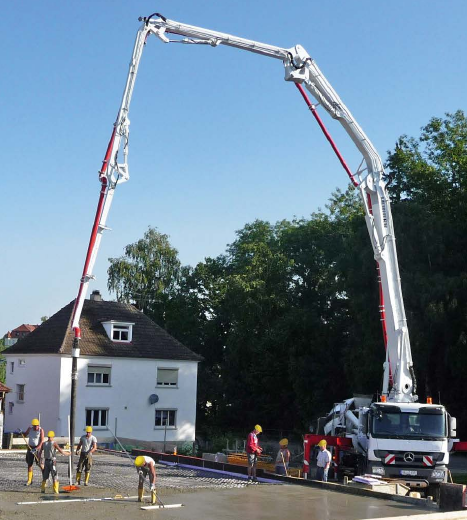
\includegraphics[scale=0.6]{betonpumpe.png}
\caption{Mobile Betonpumpe mit ausgefahrenem Ausleger, Quelle: Liebherr}
\end{figure}

In der oberen Darstellung ist eine mobile Betonpumpe bestehend aus Ausleger und LKW-Chassis zu sehen. Der Ausleger besteht aus fünf Teilen und lässt sich über Hydraulikzylinder und eine Umlenkkinematik in verschiedene Stellungen fahren. Am Chassis ist außerdem ein  Abstützsystem angebracht, welches Kräfte, die vom Ausleger ausgehen, ableitet. Es bietet darüber hinaus auch Halt in unebenem Gelände.\\

\begin{table}[h!]
\caption{Beispielwerte der Armsegmente, welche aus gegebener Gesamtmasse und Gesamtlänge ermittelt wurden}
\label{tab:WertePumpe}
\centering
\begin{tabular}{c|c|c}
\rule[-1ex]{0pt}{2.5ex} Armsegment & Masse/kg & Länge/m \\ 
\hline \rule[-1ex]{0pt}{2.5ex} 1 & 2250 & 9 \\ 
\rule[-1ex]{0pt}{2.5ex} 2 & 1700 & 8 \\ 
\rule[-1ex]{0pt}{2.5ex} 3 & 1350 & 7 \\ 
\rule[-1ex]{0pt}{2.5ex} 4 & 900 & 7 \\ 
\rule[-1ex]{0pt}{2.5ex} 5 & 480 & 6 \\ 
\end{tabular} 
\end{table}

Tabelle \ref{tab:WertePumpe} enthält die Massen und Längen der einzelnen Segmente des Auslegers, welche aus der Gesamtmasse und Gesamtlänge abgeschätzt wurden.

\section{Probleme}
Aufgrund der Leichtbauweise und dem damit verbundenem elastischen Verhalten des Materials kommt es durch den diskontinuierlichen Pumpvorgang zum Schwingen des Auslegers. Das Problem kann mit einer aktiven oder passiven Schwingungsdämpfung minimiert werden. Die aktive Schwingungsdämpfung stellt einen geschlossenen Regelkreis dar. Die Biegung kann dabei bspw. über Dehnungsmessstreifen erfasst werden und mit einem Stellsignal auf die Hydraulikzylinder korrigiert werden. Bei der passiven Schwingungsdämpfung wird versucht, über konstruktive Maßnahmen die Schwingung zu dämpfen. Das kann z.B. durch den Einsatz von bestimmten Materialien erreicht werden. Ein anderer Ansatz ist die Verwendung von passiven Vibrations-Absorbern. 

\section{Aufgabe}
In dieser Arbeit soll lediglich die aktive Schwingungsdämpfung betrachtet werden. Es soll zum einen eine Regelung und weiterhin eine Steuerung entworfen werden, um den Aktor in verschiedene Stellungen überführen zu können. \\
Als erstes wird ein Modell, welches die Dynamik des Auslegers abbildet, gesucht. Dann soll unter Verwendung der Programmiersprache Python mit Hilfe einer Simulation der Steuerungs- und Regelungsentwurf erfolgen. Die Steuerung sorgt dafür, dass möglichst alle Gelenkwinkel der Pumpe einer vorgegeben Solltrajekorie folgen. Der Regler soll dabei mögliche Abweichungen, welche durch ein vom Entwurfsmodell abweichendes reales Streckenverhalten hervorgerufen werden können, korrigieren. 


\chapter{Modellbildung}
Im folgenden Abschnitt wird das modellierte mechanische System vorgestellt. 
Der Ausleger wird als Mehrfachpendel betrachtet. Dabei wird sich auf einen Ausleger aus vier Teilen beschränkt, da das Aufstellen der Bewegungsgleichungen später symbolisch erfolgt und bereits in diesem Fall sehr unübersichtliche Terme enstehen. Darüber hinaus wird in diesem Abschnitt erläutert, wie die Biegung der Armsegmente modelliert wird.

% Rechtfertigung der Modellbeschreibung -> Hydraulikantriebe,etc.
% genauere Erklärung der Skizze
\section{Modellierung der Biegung}
\subsection{Modellierung mit verteilten Parameter}

\begin{figure}[h!]
\centering
\def\svgscale{0.8}
\input{Biegung.pdf_tex}
\caption{Biegebalken}
\label{fig:VertPara}
\end{figure}

Die Beschreibung der Balkendynamik erfolgt im verteiltparametrischen Fall über \mbox{eine} partielle Differentialgleichung (PDGL), welche man mit Hilfe der Euler-Bernoulli-Balkentheorie herleiten kann. 

\begin{equation}
EI\dfrac{\partial^4 z(x,t)}{\partial x^4}-\mu \dfrac{\partial^2 z(x,t)}{\partial t^2} = q(x,t).
\end{equation}

Dabei ist $EI$ die Biegesteifigkeit, $q$ die Streckenlast und $\mu$ die hydrodynamische Masse.\\
Vorteile der Modellierung mit Hilfe einer PDGL ist eine relativ genaue Beschreibung der Durchbiegung. Die Nachteile sind der kompliziertere Steuerungs- und Reglerentwurf und die damit verbundene zusätzliche Einarbeitungszeit in das Thema. Außerdem ist nicht ersichtlich, ob die so entworfene Steuerung und Regelung gegenüber einem Modell mit konzentrierten Parametern einen wirklich signifikanten Performance-Gewinn bringt. Aufgrund des wesentlich komplizierteren Modells wird es wahrscheinlich auch zu längeren Simulationszeiten kommen. Darüber hinaus können die Autoren nicht abschätzen, wie aufwendig die numerische Lösung von PDGLs in Python ist, bzw. welche Bibliotheken dafür bereits existieren.


\subsection{Modellierung mit konzentrierten Parameter}
\begin{figure}[!h]
\centering
\def\svgscale{0.8}
\input{KonzParameter.pdf_tex}
\caption{Modellierung der Biegung mit konzentrierten Parametern}
\label{fig:KonzPara}
\end{figure}

Um möglichst nah an den Fall der verteilten Parameter zu kommen, müssen in einem Armsegment möglichst viele konzentrierte Feder-Dämpfer-Elemente untergebracht sein. Dabei kommt mit jedem Element eine neue verkoppelte Systemgleichung hinzu, was eine symbolische Betrachtung ab einem gewissen Punkt unüberschaubar macht, die Rechenzeit der Simulation stark erhöht und die Wahl geeigneter Parameter, sowie die Verifikation erschwert.\\
Aus Gründen der einfacheren symbolischen Handhabung und des einfacheren Steuerungs- und Reglerentwurfs wurde sich daher für die Variante mit einem konzentrierten Feder-Dämpfer-Element im Segment-Schwerpunkt entschieden.
%Skizze
\begin{figure}[h!]
\centering
\def\svgscale{0.8}
\input{Skizze.pdf_tex}
\caption{Skizze des Modells für zwei Armsegmente und Durchbiegung}
\label{fig:Skizze}
\end{figure}

% Formeln

% Wahl der Koordinaten
% Potentielle und Kinetische Koenergie
% Euler Lagrange-Formalismus
Abbildung \ref{fig:Skizze} stellt das Modell eines Verteilermasts mit zwei Armsegmenten dar. Der erste Index $i$ beschreibt den physikalisch vorhandenen $i$-ten Teil des Auslegers. Der Index $j$ steht für das $j$-te Element des $i$-ten Auslegers. Wobei $j$=2 die passiven Gelenke, welche die Biegung modellieren, beschreibt. Diese sind in der Skizze durch ein Federsymbol kenntlich gemacht. Die aktuierten Gelenke hingegen sind in grau dargestellt. In diese werden äußere Momente $\vect{\tau}$ durch die hydraulischen Antriebe eingeprägt. Es werden Relativwinkel für die Winkel $\vect{\theta}$ verwendet.\\

\paragraph{Zusammenfassung}
Für die Modellierung der Durchbiegung eines Segments wird ein zusätzliches passives Gelenk mit konzentriertem Feder- und Dämpfungsparameter verwendet.\\
Für die Geometrie werden rechteckige Hohlträger angenommen, welches für die Berechnung der Trägheitsmomente entscheidend ist.\\
Die Dynamik der Hydraulikzylinder wird vernachlässigt, um das Modell nicht noch komplizierter zu machen. In der Praxis sollten diese unbedingt berücksichtigt werden.\\
Außerdem wird angenommen, dass alle Winkel und Winkelgeschwindigkeiten über entsprechende Sensoren messbar sind.

\newpage
\section{Herleitung der Bewegungsgleichung}
Ziel ist es nun die nichtlinearen Bewegungsgleichungen mit den vorgestellten Modellannahmen zu ermitteln. Dabei wird der Euler-Lagrange-Formalismus verwendet.\\ 
Zunächst werden geeignete Koordinaten für die Beschreibung der Schwerpunktlagen der Massen gesucht. Die Schwerpunkte der Teilmassen des $i$-ten Armsegments werden kartesisch beschrieben durch die Vektoren

\begin{equation}
\vect{r_{i}}=(x_{ij},y_{ij})^T.
\end{equation}

Die Gelenke sind über starre Stabelemente mit der Länge $a_{ij}$ gekoppelt. Die Minimalkoordinaten des $i$-ten Armsegment entsprechen daher den Winkeln
\begin{equation}
\vect{\theta} = (\theta_\mathrm{11},\theta_\mathrm{12},\theta_\mathrm{21},\theta_\mathrm{22})^T.
\end{equation}

Die Euler-Lagrange-Gleichungen 2.Art lauten
\begin{equation}
\frac{\mathrm d}{\mathrm dt}\dfrac{\partial L(\vect{\theta},\vectd{\theta})}{\partial \dot{\theta}_{ij}}-\dfrac{\partial L(\vect{\theta},{\vectd{\theta}})}{\partial \theta_{ij}}=\tau_{i}-d_{i}.
\label{eq:lagr}
\end{equation}

Die Lagrange-Funktionen sind
\begin{equation}
L(\vect{\theta},{\vectd{\theta}})=T(\vect{\theta},{\vectd{\theta}})-V(\vect{\theta}).
\end{equation}
$T$ stellt hierbei die kinetische Koenergie und $V$ die potentielle Energie der Massen dar.
Die kinetische Koenergie berechnet sich zu 
\begin{equation}
T = \sum \left( \dfrac{1}{2}\cdot m_{ij}\cdot(v^2_{x,ij}+v^2_{y,ij})+\dfrac{1}{2}\cdot J_{ij}\cdot\omega_{ij}^2 \right).
\end{equation}
Man erkennt einen translatorischen und einen rotatorischen Anteil.\\
Die potentielle Energie berechnet sich zu 

\begin{equation}
V = \sum \left( m_{ij}\cdot \mathrm{g} \cdot y_{ij} + k_i \cdot \theta_{ij} \right).
\end{equation}

Die kartesischen Schwerpunktkoordinaten lassen sich über die bekannten Armsegmentlängen $a_{ij}$, Schwerpunktlängen $l_{ij}$ und die Gelenkwinkel $q_{ij}$ berechnen. Exemplarisch ergibt sich damit für die ersten zwei Masseelemente aus Abbildung \ref{fig:Skizze}:

\begin{align*}
x_\mathrm{11} &= l_\mathrm{11}\cdot \cos(\theta_\mathrm{11}) \\
y_\mathrm{11} &= l_\mathrm{11}\cdot \sin(\theta_\mathrm{11}) \\
x_\mathrm{12} &= a_\mathrm{11}\cdot \cos(\theta_\mathrm{11})+l_\mathrm{12}\cdot\cos(\theta_\mathrm{11}-\theta_\mathrm{12})\\
y_\mathrm{12} &= a_\mathrm{11}\cdot \sin(\theta_\mathrm{11})+l_\mathrm{12}\cdot\sin(\theta_\mathrm{11}-\theta_\mathrm{12})\\
 			 &\mathrel{\makebox[\widthof{=}]{\vdots}} 
\end{align*}

Man erhält dabei durch Lösung von (\ref{eq:lagr}) ein System nichtlinearer Bewegungsgleichungen, welches die allgemeine Form

\begin{equation}
\vect{M}(\vect{\theta})\cdot{\vectdd{\theta}}+\vect{C}(\vect{\theta},{\vectd{\theta}})\cdot{\vectd{\theta}}+\vect{K}\cdot\vect{\theta}+\vect{g}(\vect{\theta})=\vect{\tau}
\label{eq:BWGL}
\end{equation}

besitzt.\\
Dabei stellt $\vect{M}(\vect{\theta})$ die Massenmatrix, der Term $\vect{C}(\vect{\theta},{\vectd{\theta}})$ Zentrifugalkräfte, $\vect{K}\cdot\vect{\theta}$ die elastischen Fesselungskräfte und $\vect{g}(\vect{\theta})$ Gravitationskräfte dar.

\section{Aufstellen des Zustandsraummodells}
\label{abs:aufstellen_Zustandsmodell}
Für eine regelungstechnische Betrachtung werden die Bewegungsgleichungen nun in ein Zustandsraummodell in Regelungsnormalform überführt. Dafür werden die Zustandsvektoren


\begin{align}
\begin{aligned}
\vect{x}_\mathrm{1} = ( \theta_\mathrm{11}, ..., \theta_\mathrm{22} )^T \\
\vect{x}_\mathrm{2} = ( \dot{\theta}_\mathrm{11}, ..., \dot{\theta}_\mathrm{22} )^T 
\end{aligned}
\end{align}
sowie der Vektor für die Eingangsgrößen
\begin{align}
\vect{u} = (\tau_1, \tau_2)^T
\end{align}
eingeführt.\\
Für Simulationen muss Gleichung (\ref{eq:BWGL}) nach ${\vectdd{\theta}}$ umgestellt werden, da die Simulation die Bewegungsgleichungen über eine numerische Integration löst.

\begin{align*}
\vect{M} \cdot {\vectdd{\theta}}		 &= \vect{\tau}-\vect{C} {\vectd{\theta}}-\vect{K} \vect{\theta}-\vect{g} 			\\
\vect{M}^{-1}\cdot \vect{M} \cdot {\vectdd{\theta}} &= \vect{M}^{-1}(\vect{\tau}-\vect{C} {\vectd{\theta}}-\vect{K}\vect{\theta}-\vect{g})	\\
{\vectdd{\theta}}				 &= \vect{M}^{-1}(\vect{\tau}-\vect{C}{\vectd{\theta}}-\vect{K}\vect{\theta}-\vect{g})
\end{align*}

Dies entspricht nach Umschreiben mit Hilfe der eingeführten Zustandsgrößen:

\begin{align}
\begin{aligned}
\dot{\vect{x}}_\mathrm{1} & =  \vect{x}_\mathrm{2} \\
\dot{\vect{x}}_\mathrm{2} & =  \vect{M^{-1}}(\vect{u}- \vect{C}(\vect{x}_\mathrm{1},\vect{x}_\mathrm{2})\vect{x}_\mathrm{2}-\vect{g}(\vect{x}_\mathrm{1})-\vect{K}(\vect{x}_\mathrm{1},\vect{x}_\mathrm{2}))
\end{aligned}
\end{align}

\section{Ruhelagen}
\subsection{Unvollständig aktuiertes Modell}
Da Winkelgeschwindigkeiten und -beschleunigungen in der Ruhelage verschwinden, wird 
\begin{equation}\label{eq:uva_winkel}
{\vectdd{\theta}} = {\vectd{\theta}} \stackrel{!}{=} \vect{0}.
\end{equation}
gefordert.\\
Für die Winkel der aktiven Gelenke ergibt sich damit in der Ruhelage
\begin{align}\label{eq:uva_momente}
\begin{aligned}
\theta_\mathrm{11} = \theta^\mathrm{e}_\mathrm{11}\\
\theta_\mathrm{21} = \theta^\mathrm{e}_\mathrm{21}.
\end{aligned}
\end{align}

An dieser Stelle wird gefordert, dass die Balken starr sind. Die Annahme wird hier getroffen, um den Entwurf einer Vorsteuerung zu vereinfachen. Es wird
\begin{equation}\label{eq:uva_winkel_passiv}
\theta_\mathrm{12} = \theta_\mathrm{22} \stackrel{!}{=} 0
\end{equation}
angenommen. Es handelt sich in diesem Fall um ein vollständig aktuiertes Modell. Dieses Modell wird letztendlich für die Trajektorienplanung verwendet. Im Falle eines unteraktuierten Systems wird die Trajektorienplanung wesentlich schwerer. Die Trajektorienplanung stellt in diesem Fall ein Randwertproblem dar.

\subsection{Exakte Ruhelagen/unvollständig aktuiertes Modell}
Es gelten zunächst genauso Gleichung (\ref{eq:uva_winkel}) und (\ref{eq:uva_momente}). Allerdings gilt Gleichung (\ref{eq:uva_winkel_passiv}) nun nicht mehr. Es muss jetzt das nichtlineare Gleichungssystem  

\begin{equation}
M(\vect{\theta})\cdot{\vectdd{\theta}}+C(\vect{\theta},{\vectd{\theta}})\cdot{\vectd{\theta}}+K\cdot\vect{\theta}+g(\vect{\theta}) - \vect{\tau} = \vect{0} 
\end{equation}

nach $\tau^\mathrm{e}_\mathrm{11}$, $\tau^\mathrm{e}_\mathrm{21}$, $\theta^\mathrm{e}_\mathrm{12}$ und $\theta^\mathrm{e}_\mathrm{22}$ aufgelöst werden.

\section{Linearisierung}
Die Bewegungsgleichung liegt nach der Umformung von Abschnitt \ref{abs:aufstellen_Zustandsmodell} in der Form 

\begin{equation}
{\vectdd{\theta}} = \vect{f}(\vect{\theta},{\vectd{\theta}},\vect{\tau})
\end{equation}

vor. Sie wird über die Glieder erster Ordnung einer Taylorreihe um die Ruhelage herum approximiert. 
\begin{equation}
{{\vectddt{\theta}}} = \left. \dfrac{\partial \vect{f}}{\partial \vect{\theta}}\right|_{AP} {\vectt{\theta}} + 
\left. \dfrac{\partial \vect{f}}{\partial {\vectd{\theta}}}\right|_{AP} {{\vectdt{\theta}}} + 
\left. \dfrac{\partial \vect{f}}{\partial \vect{\tau}}\right|_{AP} {\vectt{\tau}} 
\end{equation}

Mit Hilfe der eingeführten Zustandsvariablen erhält man das folgende System: 
\begin{equation}
\left( \begin{array}{c}
\dot{\vect{x}}_\mathrm{1} \\ \hline
\dot{\vect{x}}_\mathrm{2}
\end{array}\right) 
= 
\left( \begin{array}{c|c}
\vect{0} & \vect{I} \\ \hline
-{\vecto{M}}^{-1}{\vecto{K}} & {\vecto{M}}^{-1}{\vecto{C}}
\end{array} \right) 
\left( \begin{array}{c}
\vect{x_\mathrm{1}} \\ \hline
\vect{x_\mathrm{2}}
\end{array}\right) +
\left( \begin{array}{c}
\vect{0} \\ \hline
-{{\vecto{M}}}^{-1}
\end{array} \right) 
\left( \begin{array}{c}
\vect{u_1} \\ \hline
\vect{u_2}
\end{array}\right)
\end{equation}

\section{Schwierigkeiten bei der Implementierung des Zustandsraummodells}
Wie bereits erläutert, ist für die Lösung des DGL-Systems über eine numerische Integration eine Invertierung der Matrix $\vect{M}$ notwendig. Zunächst werden einige Eigenschaften der Matrix aufgeführt.\\
Sie ist symmetrisch und positiv definit. D.h.
\begin{equation*}
\vect{M}(\vect{\theta}) = \vect{M}^T(\vect{\theta})
\end{equation*}
Daraus folgt, dass 

\begin{equation*}
\det{\vect{M}(\vect{\theta})}\neq 0
\end{equation*}
und damit die Matrix invertierbar ist. Bei der symbolischen Invertierung war das Problem, dass die Matrixelemente für vier Gelenke bereits sehr lange symbolische Ausdrücke enthalten. Im folgenden sind die Anzahl an Operatoren, die in jedem Matrixelement standen, angegeben.
\begin{equation*}
\bf{COUNT\_OPERATORS(\vect{M})} = \left( \begin{array}{cccc}
195 & 161 & 114 & 59 \\
155 & 132 & 98 & 51 \\
106 & 94 & 71 & 41 \\
53 & 47 & 39 & 20 
\end{array} \right)
\end{equation*}
Nach der Linearisierung kommen noch mehr Operatoren hinzu. Daher ist eine Invertierung in symbolischer Form, aufgrund eines sehr hohen Zeitaufwandes, kaum möglich. Ein Weg die Matrix trotzdem symbolisch zu invertieren, ist die Invertierung mit Hilfe der Cholesky-Zerlegung, die im nachfolgenden Abschnitt genauer erläutert wird. \\
Schlussendlich wurde die Invertierung numerisch durchgeführt. 
\section{Cholesky-Zerlegung}
In einer Anordnung von $n$ seriellen Manipulatoren sind $2n$-Freiheitsgerade, welche die Dimension von ${M}\in\Reals^{2n\times 2n}$ beschreiben. Zur Umstellung des Gleichungssystems (\ref{eq:BWGL}) ist die Inverse der Matrix notwendig. Bei der symbolischen Implementierungen ist an dieser Stelle ein sehr hoher Rechenaufwand zu erwarten. Jede Massenmatrix eines solchen mechanischen Systems ist symmetrisch (${M}={M}^T$) und positiv definit ($\forall$ EW $>0$) \cite{janschek2009systementwurf}, eine Invertierung ist dadurch immer möglich. Durch diese Eigenschaften lässt sich eine Cholesky-Zerlegung ${M}={L}{L}^T$ (mit ${L}$ untere Dreiecksmatrix) durchführen \cite{schwarz2009numerische}. Wenn man die Multiplikation 
\begin{equation}
\begin{aligned}
	{L} {L}^T &= 
	\begin{pmatrix}
		l_{11} & 0      & 0	&	\cdots & 0\\
		l_{21} & l_{22} & 0 &  &\\
		l_{31} & l_{32} & l_{33} & &\\
		\vdots & & & \ddots & 0\\
		l_{2n1} & & & & l_{2n2n}
	\end{pmatrix} \cdot 
	\begin{pmatrix}
	l_{11} & l_{21}      & l_{31}	&	\cdots & l_{2n1}\\
	0 & l_{22} & l_{32} & &\\
	0 & 0 & l_{33} & &\\
	\vdots & & & \ddots& 0\\
	0 & & & & l_{2n2n} 
	\end{pmatrix}\\
	&= 
	\begin{pmatrix}
	l_{11}^2 & l_{21}l_{11}      & l_{31}l_{11}	&	\cdots\\
	l_{21}l_{11} & l_{21}^2+l_{22}^2 & l_{21}l_{31}+l_{22}l_{32} & \\
	l_{31}l_{11} & l_{31}l_{21}+l_{32}l_{22} & l_{31}^2+l_{32}^2+l_{33}^2 & \\
	\vdots & & & \ddots 
	\end{pmatrix}
\end{aligned}
\end{equation}

betrachtet, können durch einen Koeffizientenvergleich mit
\begin{equation}
{M}=\begin{pmatrix}
m_{11} & m_{12}      & m_{13}	&	\cdots& m_{12n}\\
m_{21} & m_{22} & m_{23} & &\\
m_{31} & m_{32} & m_{33} & &\\
\vdots & & & \ddots & \\
m_{2n1}& & & & m_{2n2n}
\end{pmatrix}
\end{equation}

die Elemente $l_{ij}$ mit $i,j=1,2,\dots,2n$ in folgender Weise berechnet werden

\begin{equation}
\begin{aligned}
	l_{ij}=
	\begin{cases}
	0, j>i\\
	\sqrt{m_{ii}-\sum \limits_{k=1}^{j-1}l^{2}_{ik}} , i=j\\
	\frac{1}{l_{jj}} \left( m_{ij}-\sum \limits_{k=1}^{j-1}l_{ik}l_{jk}\right) , i>j
	\end{cases}
\end{aligned}
\end{equation}

An dieser Stelle ist zu erahnen, dass die Wurzel nur in jedem Fall reell gelöst werden kann, wenn die zuvor genannten Eigenschaften der Matrix gelten.

Die für die allgemeine Invertierung einer Matrix  $$ A^{-1} = \dfrac{1}{\det A}(A_{\mathrm{adj}})^{T}$$zu berechnende Determinante ist durch diese Zerlegung stark vereinfacht worden. Bei einer Dreiecksmatrix haben nur die Diagonalelemente der Matrix einen Einfluss, da alle anderen Summanden nach der Regel von Sarrus Null ergeben. Außerdem gilt $$\det({L} {L}^T)=\det{L}\cdot\det{L}^T.$$ Das Produkt der Diagonalelemente von ${L}$ und das ihrer Transponierten sind identisch, so dass $\det({L} {L}^T)=(\det{L})^2$ ist.


%\chapter{Einleitung}
%%Einleitung
%Thema
%Erläuterung des Problems
%Aufgabe/Ziel
In dieser Seminararbeit soll eine verfahrbare Pumpe zur Beförderung von flüssigem Beton, wie sie im Baubereich eingesetzt wird, aus regelungstechnischer Sicht untersucht werden. Eine solche Autobetonpumpe ist in der folgenden Abbildung dargestellt. 

%Grafik
\begin{figure}[h!]
\centering
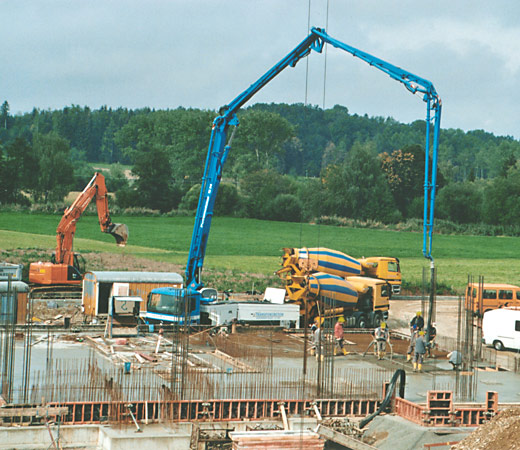
\includegraphics[scale=0.75]{betonpumpe-004.jpg}
\caption[]{Autobetonpumpe mit ausgefahrem Verteilermast, Quelle: \\http://www.trans-beton.de/images/picts/betonpumpe-004.jpg}
\end{figure}

Als erstes soll ein dynamisches Modell für die Pumpe gefunden werden. Dann soll mit Hilfe von numerischer Berechnungen/Simulationen unter Verwendung der Programmiersprache Python der Steuerungsentwurf erfolgen. Alle Gelenkwinkel der Pumpe sollen dabei möglichst exakt einer vorgegeben Solltrajekorie folgen.
Beim Einsatz der Pumpe kommt es darüberhinaus zu starken Schwingungen, welche durch einen Regler verringert werden sollen.

%\begin{figure}[h!]
%\centering
%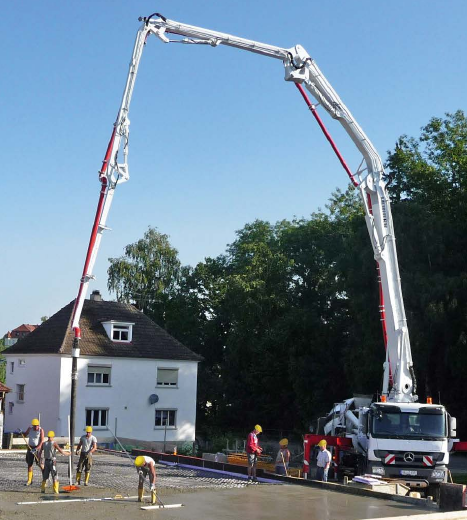
\includegraphics[scale=0.23]{betonpumpe.jpg}
%\caption[]{Betonpumpe, Quelle: \\http://i00.i.aliimg.com/photo/v1/112691528/Truck_mounted_Concrete_Boom_Pump.jpg}
%\end{figure}


\chapter{Modellbildung}
Die Anordnung soll als Mehrfachpendel modelliert werden. Die Masse der Armsegmente wird als konzentriert in den einzelnen Schwerpunkten angenommen. Die Durchbiegung eines Armsegments wird durch ein unaktuiertes Gelenk mit einer Federsteifigkeit $k$ modelliert. Auf eine verteiltparametrische Beschreibung soll verzichtet werden.
% Rechtfertigung der Modellbeschreibung -> Hydraulikantriebe,etc.
% genauere Erklärung der Skizze

%Skizze
\begin{figure}[h!]
\centering
\def\svgscale{0.8}
\input{Skizze.pdf_tex}
\caption{Skizze des Modells für zwei Armsegmente und Durchbiegung}
\label{fig:Skizze}
\end{figure}

% Formeln

% Wahl der Koordinaten
% Potentielle und Kinetische Koenergie
% Euler Lagrange-Formalismus
Abbildung \ref{fig:Skizze} stellt das Modell eines Verteilermasts mit 2 Armsegmenten dar. Der erste Index beschreibt das physikalisch vorhandene i-te Armsegment des Verteilermasts. Der zweite Index nur für die Modellierung der Biegung vorhandene Unterteilung der einzelnen Segmente. Die aktuierten Gelenke sind in grau dargestellt. In diese werden äußere Momente $F$ durch die hydraulische Antriebe eingeprägt. Die restlichen Gelenke dienen nur zur Modellierung der Biegung der Armsegmente. Alle Gelenke sind masselos. Es werden Relativwinkel zwischen den Segmenten verwendet.\\
\section{Herleitung der Bewegungsgleichung}
Ziel ist es die nichtlinearen Bewegungsgleichungen für ein Modell mit beliebig vielen Gelenkwinkel aufzustellen. Für die Herleitung der Bewegungsgleichung wird der Euler-Lagrange-Formalismus verwendet.\\ 
Zunächst werden geeignete Koordinaten für die Beschreibung der Schwerpunktlagen der Massen gesucht. Die Schwerpunkte der Teilmassen des i-ten Armsegments werden kartesisch beschrieben durch die Vektoren

\begin{equation}
\vec{x_\mathrm{i}}=(x_\mathrm{ij},y_\mathrm{ij})^T.
\end{equation}

Die Gelenke sind über starre Stabelemente mit der Länge $a_\mathrm{ij}$ gekoppelt. Die Minimalkoordinaten des i-ten Armsegment entsprechen daher den Winkeln
\begin{equation}
\vec{q_\mathrm{i}} = (q_\mathrm{i1},...,q_\mathrm{ij})^T.
\end{equation}

Die Euler-Lagrange-Gleichungen 2.Art lauten
\begin{equation}
\dfrac{d}{dt}\dfrac{\partial L(\vec{q},\dot{\vec{q}})}{q_\mathrm{ij}}-\dfrac{\partial L(\vec{q},\dot{\vec{q}})}{q_\mathrm{ij}}=F_\mathrm{i}-d_\mathrm{i}
\label{eq:lagr}
\end{equation}

mit der Lagrange-Funktion
\begin{equation}
L(\vec{q},\dot{\vec{q}})=T(\vec{q},\dot{\vec{q}})-U(\vec{q})
\end{equation}
wobei $T$ die kinetische Koenergie und $U$ die potentielle Energie der Massen darstellt.
Die kinetische Koenergie berechnet sich zu 
\begin{equation}
T = \sum \left( \dfrac{1}{2}\cdot m_\mathrm{ij}\cdot(v^2_{x,ij}+v^2_\mathrm{y,ij})+\dfrac{1}{2}\cdot J_{ij}\cdot\omega_\mathrm{ij}^2 \right).
\end{equation}
Sie enthält einen translatorischen und einen rotatorischen Anteil.\\
Die potentielle Energie berechnet sich zu 

\begin{equation}
U = \sum \left( m_\mathrm{ij}\cdot g \cdot y_\mathrm{ij} + k_i \cdot q_\mathrm{ij} \right).
\end{equation}

Die kartesischen Schwerpunktkoordinaten lassen sich über die bekannten Armsegmentlängen $a_\mathrm{ij}$, Schwerpunktlängen $l_\mathrm{ij}$ und die Gelenkwinkel $q_\mathrm{ij}$ berechnen. Exemplarisch ergibt sich damit für die ersten zwei Masseelemente aus Abbildung \ref{fig:Skizze}:

\begin{align*}
x_\mathrm{11} &= l_\mathrm{11}\cdot \cos(q_\mathrm{11}) \\
y_\mathrm{11} &= l_\mathrm{11}\cdot \sin(q_\mathrm{11}) \\
x_\mathrm{12} &= a_\mathrm{11}\cdot \cos(q_\mathrm{11})+l_\mathrm{12}\cdot\cos(q_\mathrm{11}-q_\mathrm{12})\\
y_\mathrm{12} &= a_\mathrm{11}\cdot \sin(q_\mathrm{11})+l_\mathrm{12}\cdot\sin(q_\mathrm{11}-q_\mathrm{12})\\
 			 &\mathrel{\makebox[\widthof{=}]{\vdots}} 
\end{align*}

Man erhält dabei durch Lösung von (\ref{eq:lagr}) ein System nichtlinearer Bewegungsgleichungen, welches die allgemeine Form

\begin{equation}
M(\vec{q})\cdot\ddot{\vec{q}}+C(\vec{q},\dot{\vec{q}})\cdot\dot{\vec{q}}+K\cdot\vec{q}+g(\vec{q})=\vec{F}
\label{eq:BWGL}
\end{equation}

hat. \\
Dabei stellt $M(\vec{q})$ die Massenmatrix, der Term $C(\vec{q},\dot{\vec{q}})$ Zentrifugalkräfte, $K\cdot\vec{q}$ die elastischen Fesselungskräfte und $g(\vec{q})$ Gravitationskräfte dar.\\   
Für Simulation muss (\ref{eq:BWGL}) nach $\ddot{\vec{q}}$ umgestellt werden, da diese die Bewegungsgleichungen über eine numerische Integration löst.

\begin{align*}
M \cdot \ddot{\vec{q}}		 &= \vec{F}-C\dot{\vec{q}}-K\vec{q}-g 			\\
M^{-1}\cdot M \ddot{\vec{q}} &= M^{-1}(\vec{F}-C\dot{\vec{q}}-K\vec{q}-g)	\\
\ddot{\vec{q}}				 &= M^{-1}(\vec{F}-C\dot{\vec{q}}-K\vec{q}-g)
\end{align*}

\section{Cholesky-Zerlegung}
In einer Anordnung von $n$ seriellen Manipulatoren sind $2n$-Freiheitsgerade, welche die Dimension von ${M}\in\Reals^{2n\times 2n}$ beschreiben. Zur Umstellung des Gleichungssystems (\ref{eq:BWGL}) ist die Inverse der Matrix notwendig. Bei der symbolischen Implementierungen ist an dieser Stelle ein sehr hoher Rechenaufwand zu erwarten. Jede Massenmatrix eines solchen mechanischen Systems ist symmetrisch (${M}={M}^T$) und positiv definit ($\forall$ EW $>0$) \cite{janschek2009systementwurf}, eine Invertierung ist dadurch immer möglich. Durch diese Eigenschaften lässt sich eine Cholesky-Zerlegung ${M}={L}{L}^T$ (mit ${L}$ untere Dreiecksmatrix) durchführen \cite{schwarz2009numerische}. Wenn man die Multiplikation 
\begin{equation}
\begin{aligned}
	{L} {L}^T &= 
	\begin{pmatrix}
		l_{11} & 0      & 0	&	\cdots & 0\\
		l_{21} & l_{22} & 0 &  &\\
		l_{31} & l_{32} & l_{33} & &\\
		\vdots & & & \ddots & 0\\
		l_{2n1} & & & & l_{2n2n}
	\end{pmatrix} \cdot 
	\begin{pmatrix}
	l_{11} & l_{21}      & l_{31}	&	\cdots & l_{2n1}\\
	0 & l_{22} & l_{32} & &\\
	0 & 0 & l_{33} & &\\
	\vdots & & & \ddots& 0\\
	0 & & & & l_{2n2n} 
	\end{pmatrix}\\
	&= 
	\begin{pmatrix}
	l_{11}^2 & l_{21}l_{11}      & l_{31}l_{11}	&	\cdots\\
	l_{21}l_{11} & l_{21}^2+l_{22}^2 & l_{21}l_{31}+l_{22}l_{32} & \\
	l_{31}l_{11} & l_{31}l_{21}+l_{32}l_{22} & l_{31}^2+l_{32}^2+l_{33}^2 & \\
	\vdots & & & \ddots 
	\end{pmatrix}
\end{aligned}
\end{equation}

betrachtet, können durch einen Koeffizientenvergleich mit
\begin{equation}
{M}=\begin{pmatrix}
m_{11} & m_{12}      & m_{13}	&	\cdots& m_{12n}\\
m_{21} & m_{22} & m_{23} & &\\
m_{31} & m_{32} & m_{33} & &\\
\vdots & & & \ddots & \\
m_{2n1}& & & & m_{2n2n}
\end{pmatrix}
\end{equation}

die Elemente $l_{ij}$ mit $i,j=1,2,\dots,2n$ in folgender Weise berechnet werden

\begin{equation}
\begin{aligned}
	l_{ij}=
	\begin{cases}
	0, j>i\\
	\sqrt{m_{ii}-\sum \limits_{k=1}^{j-1}l^{2}_{ik}} , i=j\\
	\frac{1}{l_{jj}} \left( m_{ij}-\sum \limits_{k=1}^{j-1}l_{ik}l_{jk}\right) , i>j
	\end{cases}
\end{aligned}
\end{equation}

An dieser Stelle ist zu erahnen, dass die Wurzel nur in jedem Fall reell gelöst werden kann, wenn die zuvor genannten Eigenschaften der Matrix gelten.

Die für die allgemeine Invertierung einer Matrix  $$ A^{-1} = \dfrac{1}{\det A}(A_{\mathrm{adj}})^{T}$$zu berechnende Determinante ist durch diese Zerlegung stark vereinfacht worden. Bei einer Dreiecksmatrix haben nur die Diagonalelemente der Matrix einen Einfluss, da alle anderen Summanden nach der Regel von Sarrus Null ergeben. Außerdem gilt $$\det({L} {L}^T)=\det{L}\cdot\det{L}^T.$$ Das Produkt der Diagonalelemente von ${L}$ und das ihrer Transponierten sind identisch, so dass $\det({L} {L}^T)=(\det{L})^2$ ist.



\chapter{Steuerungsentwurf}
 
\begin{figure}[h!]
\centering
\input{Vorsteuerung.pdf_tex}
\caption{Regelkreis}
\end{figure}

Planung einer Trajektorie. Allg Darstellung als Polynom n-ten Grades

\begin{figure}[h!]
\centering
\input{Trajektorie.pdf_tex}
\caption{Trajektorie}
\end{figure}

\begin{equation}
q_{\mathrm{traj}}(t) = a_\mathrm{n}t^n+\dots+a_\mathrm{1}t+a_\mathrm{0}
\end{equation}
Randbedingungen

\begin{align*}
q(T_\mathrm{0})			&=q_\mathrm{a} & q(T_\mathrm{1})&=q_\mathrm{soll}\\	
\dot{q}(T_\mathrm{0})	&=0 		   & \dot{q}(T_\mathrm{1})&=0\\
\ddot{q}(T_\mathrm{0})	&=0 		   & \ddot{q}(T_\mathrm{1})&=0
\end{align*}

damit lässt sich ein lineares Gleichungssystem mit 6 Gleichungen aufstellen. Es ergibt sich also ein Polynom 6.Grades.\\
Mit Hilfe der ermittelten Trajektorie für die Gelenkwinkel und der ersten und zweiten Ableitung, die berechnet werden können, können mit (\ref{eq:BWGL}) die erforderlichen Momente berechnet werden, welche die Motoren aufbringen müssen.

\begin{equation}
F_\mathrm{Vorst} = M(\vec{q}_{\mathrm{traj}})\cdot\ddot{\vec{q}}_{\mathrm{traj}}+C(\vec{q}_{\mathrm{traj}},\dot{\vec{q}}_{\mathrm{traj}})\cdot\dot{\vec{q}}_{\mathrm{traj}}+K\cdot{\vec{q}}_{\mathrm{traj}}+g(\vec{q}_{\mathrm{traj}}) 
\end{equation}

Die folgende Abbildung zeigen die Simulationsergebnisse bei Verwendung einer reinen Steuerung bei vier vorhanden Gelenkwinkel, von denen zwei aktuiert sind. 
\begin{figure}[h!]
\centering
\scalebox{0.75}{%% Creator: Matplotlib, PGF backend
%%
%% To include the figure in your LaTeX document, write
%%   \input{<filename>.pgf}
%%
%% Make sure the required packages are loaded in your preamble
%%   \usepackage{pgf}
%%
%% Figures using additional raster images can only be included by \input if
%% they are in the same directory as the main LaTeX file. For loading figures
%% from other directories you can use the `import` package
%%   \usepackage{import}
%% and then include the figures with
%%   \import{<path to file>}{<filename>.pgf}
%%
%% Matplotlib used the following preamble
%%   \usepackage{fontspec}
%%   \setsansfont{DejaVu Sans}
%%   \setmonofont{DejaVu Sans Mono}
%%
\begingroup%
\makeatletter%
\begin{pgfpicture}%
\pgfpathrectangle{\pgfpointorigin}{\pgfqpoint{8.000000in}{6.000000in}}%
\pgfusepath{use as bounding box}%
\begin{pgfscope}%
\pgfsetbuttcap%
\pgfsetroundjoin%
\definecolor{currentfill}{rgb}{1.000000,1.000000,1.000000}%
\pgfsetfillcolor{currentfill}%
\pgfsetlinewidth{0.000000pt}%
\definecolor{currentstroke}{rgb}{1.000000,1.000000,1.000000}%
\pgfsetstrokecolor{currentstroke}%
\pgfsetdash{}{0pt}%
\pgfpathmoveto{\pgfqpoint{0.000000in}{0.000000in}}%
\pgfpathlineto{\pgfqpoint{8.000000in}{0.000000in}}%
\pgfpathlineto{\pgfqpoint{8.000000in}{6.000000in}}%
\pgfpathlineto{\pgfqpoint{0.000000in}{6.000000in}}%
\pgfpathclose%
\pgfusepath{fill}%
\end{pgfscope}%
\begin{pgfscope}%
\pgfsetbuttcap%
\pgfsetroundjoin%
\definecolor{currentfill}{rgb}{1.000000,1.000000,1.000000}%
\pgfsetfillcolor{currentfill}%
\pgfsetlinewidth{0.000000pt}%
\definecolor{currentstroke}{rgb}{0.000000,0.000000,0.000000}%
\pgfsetstrokecolor{currentstroke}%
\pgfsetstrokeopacity{0.000000}%
\pgfsetdash{}{0pt}%
\pgfpathmoveto{\pgfqpoint{1.000000in}{0.600000in}}%
\pgfpathlineto{\pgfqpoint{7.200000in}{0.600000in}}%
\pgfpathlineto{\pgfqpoint{7.200000in}{5.400000in}}%
\pgfpathlineto{\pgfqpoint{1.000000in}{5.400000in}}%
\pgfpathclose%
\pgfusepath{fill}%
\end{pgfscope}%
\begin{pgfscope}%
\pgfpathrectangle{\pgfqpoint{1.000000in}{0.600000in}}{\pgfqpoint{6.200000in}{4.800000in}} %
\pgfusepath{clip}%
\pgfsetrectcap%
\pgfsetroundjoin%
\pgfsetlinewidth{1.003750pt}%
\definecolor{currentstroke}{rgb}{0.000000,0.000000,1.000000}%
\pgfsetstrokecolor{currentstroke}%
\pgfsetdash{}{0pt}%
\pgfpathmoveto{\pgfqpoint{1.000000in}{1.496000in}}%
\pgfpathlineto{\pgfqpoint{1.012401in}{1.497036in}}%
\pgfpathlineto{\pgfqpoint{1.039684in}{1.501310in}}%
\pgfpathlineto{\pgfqpoint{1.055186in}{1.502128in}}%
\pgfpathlineto{\pgfqpoint{1.082468in}{1.506045in}}%
\pgfpathlineto{\pgfqpoint{1.097970in}{1.506664in}}%
\pgfpathlineto{\pgfqpoint{1.124632in}{1.510206in}}%
\pgfpathlineto{\pgfqpoint{1.140754in}{1.510634in}}%
\pgfpathlineto{\pgfqpoint{1.166797in}{1.513756in}}%
\pgfpathlineto{\pgfqpoint{1.182918in}{1.513942in}}%
\pgfpathlineto{\pgfqpoint{1.208961in}{1.516663in}}%
\pgfpathlineto{\pgfqpoint{1.224462in}{1.516612in}}%
\pgfpathlineto{\pgfqpoint{1.251125in}{1.518886in}}%
\pgfpathlineto{\pgfqpoint{1.265387in}{1.518663in}}%
\pgfpathlineto{\pgfqpoint{1.292049in}{1.520496in}}%
\pgfpathlineto{\pgfqpoint{1.305691in}{1.520112in}}%
\pgfpathlineto{\pgfqpoint{1.331733in}{1.521489in}}%
\pgfpathlineto{\pgfqpoint{1.345375in}{1.520966in}}%
\pgfpathlineto{\pgfqpoint{1.369557in}{1.521972in}}%
\pgfpathlineto{\pgfqpoint{1.385059in}{1.521321in}}%
\pgfpathlineto{\pgfqpoint{1.403040in}{1.522354in}}%
\pgfpathlineto{\pgfqpoint{1.427843in}{1.521658in}}%
\pgfpathlineto{\pgfqpoint{1.437764in}{1.521960in}}%
\pgfpathlineto{\pgfqpoint{1.460086in}{1.520690in}}%
\pgfpathlineto{\pgfqpoint{1.479308in}{1.520784in}}%
\pgfpathlineto{\pgfqpoint{1.495430in}{1.520068in}}%
\pgfpathlineto{\pgfqpoint{1.512791in}{1.520826in}}%
\pgfpathlineto{\pgfqpoint{1.530773in}{1.519604in}}%
\pgfpathlineto{\pgfqpoint{1.556816in}{1.520199in}}%
\pgfpathlineto{\pgfqpoint{1.569217in}{1.519963in}}%
\pgfpathlineto{\pgfqpoint{1.595880in}{1.521287in}}%
\pgfpathlineto{\pgfqpoint{1.608281in}{1.521175in}}%
\pgfpathlineto{\pgfqpoint{1.638664in}{1.523213in}}%
\pgfpathlineto{\pgfqpoint{1.650445in}{1.523681in}}%
\pgfpathlineto{\pgfqpoint{1.677108in}{1.526612in}}%
\pgfpathlineto{\pgfqpoint{1.691369in}{1.527137in}}%
\pgfpathlineto{\pgfqpoint{1.721752in}{1.531077in}}%
\pgfpathlineto{\pgfqpoint{1.734153in}{1.532160in}}%
\pgfpathlineto{\pgfqpoint{1.763296in}{1.537016in}}%
\pgfpathlineto{\pgfqpoint{1.776938in}{1.538636in}}%
\pgfpathlineto{\pgfqpoint{1.806081in}{1.544513in}}%
\pgfpathlineto{\pgfqpoint{1.819102in}{1.546519in}}%
\pgfpathlineto{\pgfqpoint{1.850725in}{1.553891in}}%
\pgfpathlineto{\pgfqpoint{1.862506in}{1.556405in}}%
\pgfpathlineto{\pgfqpoint{1.891029in}{1.564461in}}%
\pgfpathlineto{\pgfqpoint{1.904050in}{1.567400in}}%
\pgfpathlineto{\pgfqpoint{1.936914in}{1.577604in}}%
\pgfpathlineto{\pgfqpoint{1.948695in}{1.581197in}}%
\pgfpathlineto{\pgfqpoint{1.973497in}{1.590403in}}%
\pgfpathlineto{\pgfqpoint{1.990239in}{1.595322in}}%
\pgfpathlineto{\pgfqpoint{2.017522in}{1.606042in}}%
\pgfpathlineto{\pgfqpoint{2.032403in}{1.610968in}}%
\pgfpathlineto{\pgfqpoint{2.060306in}{1.622476in}}%
\pgfpathlineto{\pgfqpoint{2.074567in}{1.627586in}}%
\pgfpathlineto{\pgfqpoint{2.101850in}{1.639371in}}%
\pgfpathlineto{\pgfqpoint{2.116112in}{1.644595in}}%
\pgfpathlineto{\pgfqpoint{2.145255in}{1.657470in}}%
\pgfpathlineto{\pgfqpoint{2.158896in}{1.662758in}}%
\pgfpathlineto{\pgfqpoint{2.186799in}{1.675684in}}%
\pgfpathlineto{\pgfqpoint{2.201060in}{1.681330in}}%
\pgfpathlineto{\pgfqpoint{2.232063in}{1.696182in}}%
\pgfpathlineto{\pgfqpoint{2.244464in}{1.701885in}}%
\pgfpathlineto{\pgfqpoint{2.272987in}{1.717062in}}%
\pgfpathlineto{\pgfqpoint{2.284768in}{1.723314in}}%
\pgfpathlineto{\pgfqpoint{2.330033in}{1.753848in}}%
\pgfpathlineto{\pgfqpoint{2.343674in}{1.763310in}}%
\pgfpathlineto{\pgfqpoint{2.357316in}{1.771734in}}%
\pgfpathlineto{\pgfqpoint{2.380878in}{1.787139in}}%
\pgfpathlineto{\pgfqpoint{2.397000in}{1.795670in}}%
\pgfpathlineto{\pgfqpoint{2.420562in}{1.809641in}}%
\pgfpathlineto{\pgfqpoint{2.437924in}{1.817947in}}%
\pgfpathlineto{\pgfqpoint{2.463346in}{1.832336in}}%
\pgfpathlineto{\pgfqpoint{2.480088in}{1.840142in}}%
\pgfpathlineto{\pgfqpoint{2.506131in}{1.854625in}}%
\pgfpathlineto{\pgfqpoint{2.522872in}{1.862255in}}%
\pgfpathlineto{\pgfqpoint{2.547675in}{1.875632in}}%
\pgfpathlineto{\pgfqpoint{2.566897in}{1.883722in}}%
\pgfpathlineto{\pgfqpoint{2.587359in}{1.893853in}}%
\pgfpathlineto{\pgfqpoint{2.615882in}{1.904123in}}%
\pgfpathlineto{\pgfqpoint{2.627663in}{1.908378in}}%
\pgfpathlineto{\pgfqpoint{2.671067in}{1.917110in}}%
\pgfpathlineto{\pgfqpoint{2.697730in}{1.918039in}}%
\pgfpathlineto{\pgfqpoint{2.705791in}{1.917638in}}%
\pgfpathlineto{\pgfqpoint{2.732453in}{1.914183in}}%
\pgfpathlineto{\pgfqpoint{2.743614in}{1.913558in}}%
\pgfpathlineto{\pgfqpoint{2.757256in}{1.912365in}}%
\pgfpathlineto{\pgfqpoint{2.767177in}{1.913707in}}%
\pgfpathlineto{\pgfqpoint{2.783298in}{1.916192in}}%
\pgfpathlineto{\pgfqpoint{2.798800in}{1.918017in}}%
\pgfpathlineto{\pgfqpoint{2.811201in}{1.922326in}}%
\pgfpathlineto{\pgfqpoint{2.825463in}{1.926683in}}%
\pgfpathlineto{\pgfqpoint{2.842204in}{1.931398in}}%
\pgfpathlineto{\pgfqpoint{2.891189in}{1.953494in}}%
\pgfpathlineto{\pgfqpoint{2.909791in}{1.963559in}}%
\pgfpathlineto{\pgfqpoint{2.929633in}{1.972969in}}%
\pgfpathlineto{\pgfqpoint{2.955676in}{1.987782in}}%
\pgfpathlineto{\pgfqpoint{2.971177in}{1.995616in}}%
\pgfpathlineto{\pgfqpoint{2.997840in}{2.011056in}}%
\pgfpathlineto{\pgfqpoint{3.013961in}{2.019224in}}%
\pgfpathlineto{\pgfqpoint{3.039384in}{2.034029in}}%
\pgfpathlineto{\pgfqpoint{3.056126in}{2.042388in}}%
\pgfpathlineto{\pgfqpoint{3.083408in}{2.058317in}}%
\pgfpathlineto{\pgfqpoint{3.097670in}{2.065837in}}%
\pgfpathlineto{\pgfqpoint{3.172697in}{2.115837in}}%
\pgfpathlineto{\pgfqpoint{3.193779in}{2.132466in}}%
\pgfpathlineto{\pgfqpoint{3.212381in}{2.144130in}}%
\pgfpathlineto{\pgfqpoint{3.231603in}{2.157174in}}%
\pgfpathlineto{\pgfqpoint{3.252685in}{2.168814in}}%
\pgfpathlineto{\pgfqpoint{3.273147in}{2.181642in}}%
\pgfpathlineto{\pgfqpoint{3.293609in}{2.192335in}}%
\pgfpathlineto{\pgfqpoint{3.315932in}{2.206133in}}%
\pgfpathlineto{\pgfqpoint{3.335154in}{2.216065in}}%
\pgfpathlineto{\pgfqpoint{3.359336in}{2.230936in}}%
\pgfpathlineto{\pgfqpoint{3.377938in}{2.240469in}}%
\pgfpathlineto{\pgfqpoint{3.400880in}{2.254177in}}%
\pgfpathlineto{\pgfqpoint{3.422582in}{2.264456in}}%
\pgfpathlineto{\pgfqpoint{3.439944in}{2.273836in}}%
\pgfpathlineto{\pgfqpoint{3.485829in}{2.290173in}}%
\pgfpathlineto{\pgfqpoint{3.509391in}{2.294733in}}%
\pgfpathlineto{\pgfqpoint{3.519312in}{2.296445in}}%
\pgfpathlineto{\pgfqpoint{3.532953in}{2.295462in}}%
\pgfpathlineto{\pgfqpoint{3.544114in}{2.295308in}}%
\pgfpathlineto{\pgfqpoint{3.555896in}{2.294949in}}%
\pgfpathlineto{\pgfqpoint{3.575738in}{2.293543in}}%
\pgfpathlineto{\pgfqpoint{3.589999in}{2.296681in}}%
\pgfpathlineto{\pgfqpoint{3.615422in}{2.301941in}}%
\pgfpathlineto{\pgfqpoint{3.659446in}{2.322080in}}%
\pgfpathlineto{\pgfqpoint{3.682388in}{2.335976in}}%
\pgfpathlineto{\pgfqpoint{3.696650in}{2.344301in}}%
\pgfpathlineto{\pgfqpoint{3.784078in}{2.408178in}}%
\pgfpathlineto{\pgfqpoint{3.806401in}{2.427337in}}%
\pgfpathlineto{\pgfqpoint{3.819422in}{2.438782in}}%
\pgfpathlineto{\pgfqpoint{3.841124in}{2.461223in}}%
\pgfpathlineto{\pgfqpoint{3.860966in}{2.480772in}}%
\pgfpathlineto{\pgfqpoint{3.871507in}{2.490225in}}%
\pgfpathlineto{\pgfqpoint{3.930413in}{2.534488in}}%
\pgfpathlineto{\pgfqpoint{3.963896in}{2.558120in}}%
\pgfpathlineto{\pgfqpoint{3.979398in}{2.568487in}}%
\pgfpathlineto{\pgfqpoint{3.996140in}{2.579529in}}%
\pgfpathlineto{\pgfqpoint{4.042644in}{2.602231in}}%
\pgfpathlineto{\pgfqpoint{4.062486in}{2.608559in}}%
\pgfpathlineto{\pgfqpoint{4.076128in}{2.612323in}}%
\pgfpathlineto{\pgfqpoint{4.086049in}{2.612450in}}%
\pgfpathlineto{\pgfqpoint{4.100930in}{2.613279in}}%
\pgfpathlineto{\pgfqpoint{4.112711in}{2.613137in}}%
\pgfpathlineto{\pgfqpoint{4.129453in}{2.611866in}}%
\pgfpathlineto{\pgfqpoint{4.167277in}{2.618657in}}%
\pgfpathlineto{\pgfqpoint{4.206341in}{2.634881in}}%
\pgfpathlineto{\pgfqpoint{4.219982in}{2.643492in}}%
\pgfpathlineto{\pgfqpoint{4.236104in}{2.652698in}}%
\pgfpathlineto{\pgfqpoint{4.250985in}{2.661505in}}%
\pgfpathlineto{\pgfqpoint{4.286949in}{2.686318in}}%
\pgfpathlineto{\pgfqpoint{4.299970in}{2.696509in}}%
\pgfpathlineto{\pgfqpoint{4.316712in}{2.709374in}}%
\pgfpathlineto{\pgfqpoint{4.337174in}{2.723992in}}%
\pgfpathlineto{\pgfqpoint{4.363836in}{2.745808in}}%
\pgfpathlineto{\pgfqpoint{4.376238in}{2.756189in}}%
\pgfpathlineto{\pgfqpoint{4.411581in}{2.791536in}}%
\pgfpathlineto{\pgfqpoint{4.427703in}{2.809481in}}%
\pgfpathlineto{\pgfqpoint{4.440724in}{2.820247in}}%
\pgfpathlineto{\pgfqpoint{4.456226in}{2.834982in}}%
\pgfpathlineto{\pgfqpoint{4.469247in}{2.846244in}}%
\pgfpathlineto{\pgfqpoint{4.492189in}{2.864076in}}%
\pgfpathlineto{\pgfqpoint{4.510171in}{2.879300in}}%
\pgfpathlineto{\pgfqpoint{4.535594in}{2.898054in}}%
\pgfpathlineto{\pgfqpoint{4.550475in}{2.909744in}}%
\pgfpathlineto{\pgfqpoint{4.593879in}{2.935956in}}%
\pgfpathlineto{\pgfqpoint{4.627983in}{2.947838in}}%
\pgfpathlineto{\pgfqpoint{4.637904in}{2.948180in}}%
\pgfpathlineto{\pgfqpoint{4.660226in}{2.948159in}}%
\pgfpathlineto{\pgfqpoint{4.670767in}{2.947576in}}%
\pgfpathlineto{\pgfqpoint{4.679448in}{2.948171in}}%
\pgfpathlineto{\pgfqpoint{4.688749in}{2.951066in}}%
\pgfpathlineto{\pgfqpoint{4.727193in}{2.968712in}}%
\pgfpathlineto{\pgfqpoint{4.753235in}{2.986463in}}%
\pgfpathlineto{\pgfqpoint{4.765017in}{2.995292in}}%
\pgfpathlineto{\pgfqpoint{4.799740in}{3.024195in}}%
\pgfpathlineto{\pgfqpoint{4.812141in}{3.035892in}}%
\pgfpathlineto{\pgfqpoint{4.830743in}{3.053259in}}%
\pgfpathlineto{\pgfqpoint{4.846245in}{3.067333in}}%
\pgfpathlineto{\pgfqpoint{4.887169in}{3.114241in}}%
\pgfpathlineto{\pgfqpoint{4.897710in}{3.126832in}}%
\pgfpathlineto{\pgfqpoint{4.938634in}{3.166581in}}%
\pgfpathlineto{\pgfqpoint{4.965917in}{3.189894in}}%
\pgfpathlineto{\pgfqpoint{4.979558in}{3.201566in}}%
\pgfpathlineto{\pgfqpoint{5.009941in}{3.224844in}}%
\pgfpathlineto{\pgfqpoint{5.021722in}{3.233100in}}%
\pgfpathlineto{\pgfqpoint{5.063886in}{3.255607in}}%
\pgfpathlineto{\pgfqpoint{5.098610in}{3.263118in}}%
\pgfpathlineto{\pgfqpoint{5.114731in}{3.261902in}}%
\pgfpathlineto{\pgfqpoint{5.152555in}{3.269258in}}%
\pgfpathlineto{\pgfqpoint{5.186039in}{3.286205in}}%
\pgfpathlineto{\pgfqpoint{5.197820in}{3.294839in}}%
\pgfpathlineto{\pgfqpoint{5.221382in}{3.312362in}}%
\pgfpathlineto{\pgfqpoint{5.233783in}{3.322359in}}%
\pgfpathlineto{\pgfqpoint{5.267267in}{3.351840in}}%
\pgfpathlineto{\pgfqpoint{5.279668in}{3.364078in}}%
\pgfpathlineto{\pgfqpoint{5.300130in}{3.384514in}}%
\pgfpathlineto{\pgfqpoint{5.315012in}{3.400298in}}%
\pgfpathlineto{\pgfqpoint{5.348495in}{3.442299in}}%
\pgfpathlineto{\pgfqpoint{5.368337in}{3.464870in}}%
\pgfpathlineto{\pgfqpoint{5.387559in}{3.484068in}}%
\pgfpathlineto{\pgfqpoint{5.406161in}{3.502721in}}%
\pgfpathlineto{\pgfqpoint{5.430343in}{3.524426in}}%
\pgfpathlineto{\pgfqpoint{5.445845in}{3.538252in}}%
\pgfpathlineto{\pgfqpoint{5.483048in}{3.564193in}}%
\pgfpathlineto{\pgfqpoint{5.492969in}{3.568124in}}%
\pgfpathlineto{\pgfqpoint{5.522732in}{3.575639in}}%
\pgfpathlineto{\pgfqpoint{5.541334in}{3.574518in}}%
\pgfpathlineto{\pgfqpoint{5.569237in}{3.582412in}}%
\pgfpathlineto{\pgfqpoint{5.577918in}{3.587157in}}%
\pgfpathlineto{\pgfqpoint{5.615122in}{3.613880in}}%
\pgfpathlineto{\pgfqpoint{5.657906in}{3.653860in}}%
\pgfpathlineto{\pgfqpoint{5.705651in}{3.706361in}}%
\pgfpathlineto{\pgfqpoint{5.726733in}{3.733088in}}%
\pgfpathlineto{\pgfqpoint{5.755256in}{3.768612in}}%
\pgfpathlineto{\pgfqpoint{5.770757in}{3.784750in}}%
\pgfpathlineto{\pgfqpoint{5.789359in}{3.804540in}}%
\pgfpathlineto{\pgfqpoint{5.817262in}{3.830411in}}%
\pgfpathlineto{\pgfqpoint{5.829663in}{3.841739in}}%
\pgfpathlineto{\pgfqpoint{5.869347in}{3.870739in}}%
\pgfpathlineto{\pgfqpoint{5.881128in}{3.875500in}}%
\pgfpathlineto{\pgfqpoint{5.909031in}{3.884442in}}%
\pgfpathlineto{\pgfqpoint{5.935074in}{3.885828in}}%
\pgfpathlineto{\pgfqpoint{5.961116in}{3.893502in}}%
\pgfpathlineto{\pgfqpoint{5.974137in}{3.902307in}}%
\pgfpathlineto{\pgfqpoint{6.004520in}{3.924462in}}%
\pgfpathlineto{\pgfqpoint{6.058466in}{3.978852in}}%
\pgfpathlineto{\pgfqpoint{6.087609in}{4.012275in}}%
\pgfpathlineto{\pgfqpoint{6.140934in}{4.083444in}}%
\pgfpathlineto{\pgfqpoint{6.158916in}{4.104244in}}%
\pgfpathlineto{\pgfqpoint{6.172557in}{4.119129in}}%
\pgfpathlineto{\pgfqpoint{6.218442in}{4.161533in}}%
\pgfpathlineto{\pgfqpoint{6.248825in}{4.180716in}}%
\pgfpathlineto{\pgfqpoint{6.259366in}{4.182921in}}%
\pgfpathlineto{\pgfqpoint{6.276728in}{4.185040in}}%
\pgfpathlineto{\pgfqpoint{6.292849in}{4.185692in}}%
\pgfpathlineto{\pgfqpoint{6.299670in}{4.188021in}}%
\pgfpathlineto{\pgfqpoint{6.312691in}{4.195385in}}%
\pgfpathlineto{\pgfqpoint{6.339354in}{4.213408in}}%
\pgfpathlineto{\pgfqpoint{6.379658in}{4.252640in}}%
\pgfpathlineto{\pgfqpoint{6.428023in}{4.309843in}}%
\pgfpathlineto{\pgfqpoint{6.460266in}{4.355791in}}%
\pgfpathlineto{\pgfqpoint{6.470187in}{4.369244in}}%
\pgfpathlineto{\pgfqpoint{6.525993in}{4.430152in}}%
\pgfpathlineto{\pgfqpoint{6.552655in}{4.456500in}}%
\pgfpathlineto{\pgfqpoint{6.591099in}{4.482550in}}%
\pgfpathlineto{\pgfqpoint{6.618382in}{4.488966in}}%
\pgfpathlineto{\pgfqpoint{6.639464in}{4.490157in}}%
\pgfpathlineto{\pgfqpoint{6.653105in}{4.497784in}}%
\pgfpathlineto{\pgfqpoint{6.677908in}{4.513131in}}%
\pgfpathlineto{\pgfqpoint{6.720072in}{4.555071in}}%
\pgfpathlineto{\pgfqpoint{6.743634in}{4.583209in}}%
\pgfpathlineto{\pgfqpoint{6.756656in}{4.598620in}}%
\pgfpathlineto{\pgfqpoint{6.787659in}{4.645106in}}%
\pgfpathlineto{\pgfqpoint{6.806261in}{4.673857in}}%
\pgfpathlineto{\pgfqpoint{6.852765in}{4.728398in}}%
\pgfpathlineto{\pgfqpoint{6.867027in}{4.742596in}}%
\pgfpathlineto{\pgfqpoint{6.884388in}{4.760547in}}%
\pgfpathlineto{\pgfqpoint{6.893689in}{4.766104in}}%
\pgfpathlineto{\pgfqpoint{6.909191in}{4.775335in}}%
\pgfpathlineto{\pgfqpoint{6.919112in}{4.780373in}}%
\pgfpathlineto{\pgfqpoint{6.925313in}{4.780786in}}%
\pgfpathlineto{\pgfqpoint{6.940814in}{4.780942in}}%
\pgfpathlineto{\pgfqpoint{6.958796in}{4.787186in}}%
\pgfpathlineto{\pgfqpoint{6.968717in}{4.791278in}}%
\pgfpathlineto{\pgfqpoint{6.976778in}{4.797364in}}%
\pgfpathlineto{\pgfqpoint{7.013981in}{4.832062in}}%
\pgfpathlineto{\pgfqpoint{7.061106in}{4.889454in}}%
\pgfpathlineto{\pgfqpoint{7.097690in}{4.944777in}}%
\pgfpathlineto{\pgfqpoint{7.106371in}{4.957678in}}%
\pgfpathlineto{\pgfqpoint{7.149155in}{5.010810in}}%
\pgfpathlineto{\pgfqpoint{7.167757in}{5.030670in}}%
\pgfpathlineto{\pgfqpoint{7.183258in}{5.047725in}}%
\pgfpathlineto{\pgfqpoint{7.196900in}{5.057782in}}%
\pgfpathlineto{\pgfqpoint{7.200000in}{5.060078in}}%
\pgfpathlineto{\pgfqpoint{7.200000in}{5.060078in}}%
\pgfusepath{stroke}%
\end{pgfscope}%
\begin{pgfscope}%
\pgfpathrectangle{\pgfqpoint{1.000000in}{0.600000in}}{\pgfqpoint{6.200000in}{4.800000in}} %
\pgfusepath{clip}%
\pgfsetrectcap%
\pgfsetroundjoin%
\pgfsetlinewidth{1.003750pt}%
\definecolor{currentstroke}{rgb}{0.000000,0.500000,0.000000}%
\pgfsetstrokecolor{currentstroke}%
\pgfsetdash{}{0pt}%
\pgfpathmoveto{\pgfqpoint{1.000000in}{1.400000in}}%
\pgfpathlineto{\pgfqpoint{1.008681in}{1.401522in}}%
\pgfpathlineto{\pgfqpoint{1.016122in}{1.400430in}}%
\pgfpathlineto{\pgfqpoint{1.031003in}{1.397330in}}%
\pgfpathlineto{\pgfqpoint{1.038444in}{1.398663in}}%
\pgfpathlineto{\pgfqpoint{1.052085in}{1.401509in}}%
\pgfpathlineto{\pgfqpoint{1.059526in}{1.400264in}}%
\pgfpathlineto{\pgfqpoint{1.073787in}{1.397319in}}%
\pgfpathlineto{\pgfqpoint{1.081228in}{1.398661in}}%
\pgfpathlineto{\pgfqpoint{1.094249in}{1.401501in}}%
\pgfpathlineto{\pgfqpoint{1.101690in}{1.400414in}}%
\pgfpathlineto{\pgfqpoint{1.116572in}{1.397315in}}%
\pgfpathlineto{\pgfqpoint{1.124012in}{1.398709in}}%
\pgfpathlineto{\pgfqpoint{1.137034in}{1.401485in}}%
\pgfpathlineto{\pgfqpoint{1.144474in}{1.400340in}}%
\pgfpathlineto{\pgfqpoint{1.158736in}{1.397294in}}%
\pgfpathlineto{\pgfqpoint{1.166177in}{1.398657in}}%
\pgfpathlineto{\pgfqpoint{1.179198in}{1.401468in}}%
\pgfpathlineto{\pgfqpoint{1.186639in}{1.400348in}}%
\pgfpathlineto{\pgfqpoint{1.200900in}{1.397280in}}%
\pgfpathlineto{\pgfqpoint{1.208341in}{1.398723in}}%
\pgfpathlineto{\pgfqpoint{1.220742in}{1.401452in}}%
\pgfpathlineto{\pgfqpoint{1.228183in}{1.400395in}}%
\pgfpathlineto{\pgfqpoint{1.243064in}{1.397293in}}%
\pgfpathlineto{\pgfqpoint{1.250505in}{1.398971in}}%
\pgfpathlineto{\pgfqpoint{1.261666in}{1.401437in}}%
\pgfpathlineto{\pgfqpoint{1.269107in}{1.400432in}}%
\pgfpathlineto{\pgfqpoint{1.283988in}{1.397283in}}%
\pgfpathlineto{\pgfqpoint{1.291429in}{1.399092in}}%
\pgfpathlineto{\pgfqpoint{1.301970in}{1.401415in}}%
\pgfpathlineto{\pgfqpoint{1.309411in}{1.400410in}}%
\pgfpathlineto{\pgfqpoint{1.323672in}{1.397269in}}%
\pgfpathlineto{\pgfqpoint{1.331113in}{1.399161in}}%
\pgfpathlineto{\pgfqpoint{1.341034in}{1.401357in}}%
\pgfpathlineto{\pgfqpoint{1.347855in}{1.400632in}}%
\pgfpathlineto{\pgfqpoint{1.362736in}{1.397447in}}%
\pgfpathlineto{\pgfqpoint{1.385679in}{1.400663in}}%
\pgfpathlineto{\pgfqpoint{1.396840in}{1.397655in}}%
\pgfpathlineto{\pgfqpoint{1.406761in}{1.398783in}}%
\pgfpathlineto{\pgfqpoint{1.416682in}{1.401438in}}%
\pgfpathlineto{\pgfqpoint{1.428463in}{1.398831in}}%
\pgfpathlineto{\pgfqpoint{1.434663in}{1.397243in}}%
\pgfpathlineto{\pgfqpoint{1.445825in}{1.399702in}}%
\pgfpathlineto{\pgfqpoint{1.453265in}{1.401602in}}%
\pgfpathlineto{\pgfqpoint{1.466287in}{1.398234in}}%
\pgfpathlineto{\pgfqpoint{1.471247in}{1.397311in}}%
\pgfpathlineto{\pgfqpoint{1.482408in}{1.399895in}}%
\pgfpathlineto{\pgfqpoint{1.490469in}{1.401707in}}%
\pgfpathlineto{\pgfqpoint{1.502250in}{1.398646in}}%
\pgfpathlineto{\pgfqpoint{1.510931in}{1.397553in}}%
\pgfpathlineto{\pgfqpoint{1.517752in}{1.399927in}}%
\pgfpathlineto{\pgfqpoint{1.524572in}{1.401313in}}%
\pgfpathlineto{\pgfqpoint{1.533253in}{1.400640in}}%
\pgfpathlineto{\pgfqpoint{1.549375in}{1.397844in}}%
\pgfpathlineto{\pgfqpoint{1.567977in}{1.401376in}}%
\pgfpathlineto{\pgfqpoint{1.576038in}{1.399456in}}%
\pgfpathlineto{\pgfqpoint{1.585339in}{1.397462in}}%
\pgfpathlineto{\pgfqpoint{1.592159in}{1.398719in}}%
\pgfpathlineto{\pgfqpoint{1.604560in}{1.401535in}}%
\pgfpathlineto{\pgfqpoint{1.612001in}{1.400672in}}%
\pgfpathlineto{\pgfqpoint{1.628123in}{1.397651in}}%
\pgfpathlineto{\pgfqpoint{1.636184in}{1.399687in}}%
\pgfpathlineto{\pgfqpoint{1.645485in}{1.401574in}}%
\pgfpathlineto{\pgfqpoint{1.652925in}{1.400692in}}%
\pgfpathlineto{\pgfqpoint{1.669667in}{1.397734in}}%
\pgfpathlineto{\pgfqpoint{1.677728in}{1.399589in}}%
\pgfpathlineto{\pgfqpoint{1.687649in}{1.401587in}}%
\pgfpathlineto{\pgfqpoint{1.695090in}{1.400619in}}%
\pgfpathlineto{\pgfqpoint{1.711211in}{1.397792in}}%
\pgfpathlineto{\pgfqpoint{1.719272in}{1.399384in}}%
\pgfpathlineto{\pgfqpoint{1.730433in}{1.401571in}}%
\pgfpathlineto{\pgfqpoint{1.738494in}{1.400365in}}%
\pgfpathlineto{\pgfqpoint{1.752135in}{1.397798in}}%
\pgfpathlineto{\pgfqpoint{1.760196in}{1.399003in}}%
\pgfpathlineto{\pgfqpoint{1.773837in}{1.401536in}}%
\pgfpathlineto{\pgfqpoint{1.781898in}{1.400164in}}%
\pgfpathlineto{\pgfqpoint{1.794919in}{1.397791in}}%
\pgfpathlineto{\pgfqpoint{1.802980in}{1.399078in}}%
\pgfpathlineto{\pgfqpoint{1.816002in}{1.401544in}}%
\pgfpathlineto{\pgfqpoint{1.824062in}{1.400303in}}%
\pgfpathlineto{\pgfqpoint{1.837704in}{1.397749in}}%
\pgfpathlineto{\pgfqpoint{1.845765in}{1.399094in}}%
\pgfpathlineto{\pgfqpoint{1.858786in}{1.401575in}}%
\pgfpathlineto{\pgfqpoint{1.866847in}{1.400271in}}%
\pgfpathlineto{\pgfqpoint{1.880488in}{1.397705in}}%
\pgfpathlineto{\pgfqpoint{1.888549in}{1.399078in}}%
\pgfpathlineto{\pgfqpoint{1.900950in}{1.401620in}}%
\pgfpathlineto{\pgfqpoint{1.908391in}{1.400550in}}%
\pgfpathlineto{\pgfqpoint{1.923272in}{1.397677in}}%
\pgfpathlineto{\pgfqpoint{1.931333in}{1.399082in}}%
\pgfpathlineto{\pgfqpoint{1.943734in}{1.401613in}}%
\pgfpathlineto{\pgfqpoint{1.951175in}{1.400473in}}%
\pgfpathlineto{\pgfqpoint{1.965437in}{1.397637in}}%
\pgfpathlineto{\pgfqpoint{1.973497in}{1.398979in}}%
\pgfpathlineto{\pgfqpoint{1.986519in}{1.401526in}}%
\pgfpathlineto{\pgfqpoint{1.993959in}{1.400334in}}%
\pgfpathlineto{\pgfqpoint{2.007601in}{1.397588in}}%
\pgfpathlineto{\pgfqpoint{2.015662in}{1.398952in}}%
\pgfpathlineto{\pgfqpoint{2.028683in}{1.401386in}}%
\pgfpathlineto{\pgfqpoint{2.036124in}{1.400293in}}%
\pgfpathlineto{\pgfqpoint{2.050385in}{1.397567in}}%
\pgfpathlineto{\pgfqpoint{2.059066in}{1.399281in}}%
\pgfpathlineto{\pgfqpoint{2.070227in}{1.401268in}}%
\pgfpathlineto{\pgfqpoint{2.078288in}{1.400197in}}%
\pgfpathlineto{\pgfqpoint{2.092549in}{1.397535in}}%
\pgfpathlineto{\pgfqpoint{2.100610in}{1.399073in}}%
\pgfpathlineto{\pgfqpoint{2.112391in}{1.401245in}}%
\pgfpathlineto{\pgfqpoint{2.120452in}{1.400133in}}%
\pgfpathlineto{\pgfqpoint{2.134713in}{1.397526in}}%
\pgfpathlineto{\pgfqpoint{2.142774in}{1.398979in}}%
\pgfpathlineto{\pgfqpoint{2.155176in}{1.401306in}}%
\pgfpathlineto{\pgfqpoint{2.163236in}{1.400054in}}%
\pgfpathlineto{\pgfqpoint{2.176878in}{1.397530in}}%
\pgfpathlineto{\pgfqpoint{2.184938in}{1.398895in}}%
\pgfpathlineto{\pgfqpoint{2.197960in}{1.401407in}}%
\pgfpathlineto{\pgfqpoint{2.206021in}{1.400123in}}%
\pgfpathlineto{\pgfqpoint{2.219042in}{1.397563in}}%
\pgfpathlineto{\pgfqpoint{2.226483in}{1.398764in}}%
\pgfpathlineto{\pgfqpoint{2.240744in}{1.401547in}}%
\pgfpathlineto{\pgfqpoint{2.248805in}{1.400208in}}%
\pgfpathlineto{\pgfqpoint{2.261206in}{1.397724in}}%
\pgfpathlineto{\pgfqpoint{2.268027in}{1.399002in}}%
\pgfpathlineto{\pgfqpoint{2.280428in}{1.401808in}}%
\pgfpathlineto{\pgfqpoint{2.288489in}{1.400786in}}%
\pgfpathlineto{\pgfqpoint{2.303370in}{1.398275in}}%
\pgfpathlineto{\pgfqpoint{2.321972in}{1.401637in}}%
\pgfpathlineto{\pgfqpoint{2.325693in}{1.400413in}}%
\pgfpathlineto{\pgfqpoint{2.331893in}{1.397932in}}%
\pgfpathlineto{\pgfqpoint{2.344294in}{1.398542in}}%
\pgfpathlineto{\pgfqpoint{2.351115in}{1.400555in}}%
\pgfpathlineto{\pgfqpoint{2.360416in}{1.399672in}}%
\pgfpathlineto{\pgfqpoint{2.377158in}{1.397276in}}%
\pgfpathlineto{\pgfqpoint{2.393899in}{1.400886in}}%
\pgfpathlineto{\pgfqpoint{2.402580in}{1.399180in}}%
\pgfpathlineto{\pgfqpoint{2.413121in}{1.397137in}}%
\pgfpathlineto{\pgfqpoint{2.419942in}{1.398279in}}%
\pgfpathlineto{\pgfqpoint{2.433583in}{1.401299in}}%
\pgfpathlineto{\pgfqpoint{2.441024in}{1.400227in}}%
\pgfpathlineto{\pgfqpoint{2.455906in}{1.397380in}}%
\pgfpathlineto{\pgfqpoint{2.463966in}{1.398989in}}%
\pgfpathlineto{\pgfqpoint{2.475748in}{1.401438in}}%
\pgfpathlineto{\pgfqpoint{2.483188in}{1.400361in}}%
\pgfpathlineto{\pgfqpoint{2.498070in}{1.397367in}}%
\pgfpathlineto{\pgfqpoint{2.506131in}{1.398853in}}%
\pgfpathlineto{\pgfqpoint{2.518532in}{1.401377in}}%
\pgfpathlineto{\pgfqpoint{2.525973in}{1.400221in}}%
\pgfpathlineto{\pgfqpoint{2.540234in}{1.397195in}}%
\pgfpathlineto{\pgfqpoint{2.547675in}{1.398377in}}%
\pgfpathlineto{\pgfqpoint{2.561316in}{1.401153in}}%
\pgfpathlineto{\pgfqpoint{2.568757in}{1.399942in}}%
\pgfpathlineto{\pgfqpoint{2.583018in}{1.396951in}}%
\pgfpathlineto{\pgfqpoint{2.591079in}{1.398355in}}%
\pgfpathlineto{\pgfqpoint{2.603480in}{1.400847in}}%
\pgfpathlineto{\pgfqpoint{2.610921in}{1.399746in}}%
\pgfpathlineto{\pgfqpoint{2.625803in}{1.396691in}}%
\pgfpathlineto{\pgfqpoint{2.633863in}{1.398305in}}%
\pgfpathlineto{\pgfqpoint{2.645025in}{1.400491in}}%
\pgfpathlineto{\pgfqpoint{2.652465in}{1.399503in}}%
\pgfpathlineto{\pgfqpoint{2.667347in}{1.396395in}}%
\pgfpathlineto{\pgfqpoint{2.676028in}{1.398610in}}%
\pgfpathlineto{\pgfqpoint{2.685329in}{1.400064in}}%
\pgfpathlineto{\pgfqpoint{2.692149in}{1.399192in}}%
\pgfpathlineto{\pgfqpoint{2.703310in}{1.396562in}}%
\pgfpathlineto{\pgfqpoint{2.716332in}{1.400468in}}%
\pgfpathlineto{\pgfqpoint{2.720672in}{1.401709in}}%
\pgfpathlineto{\pgfqpoint{2.734933in}{1.399015in}}%
\pgfpathlineto{\pgfqpoint{2.739894in}{1.398601in}}%
\pgfpathlineto{\pgfqpoint{2.750435in}{1.401688in}}%
\pgfpathlineto{\pgfqpoint{2.759736in}{1.402500in}}%
\pgfpathlineto{\pgfqpoint{2.767177in}{1.400809in}}%
\pgfpathlineto{\pgfqpoint{2.776478in}{1.398646in}}%
\pgfpathlineto{\pgfqpoint{2.783298in}{1.399579in}}%
\pgfpathlineto{\pgfqpoint{2.797560in}{1.402392in}}%
\pgfpathlineto{\pgfqpoint{2.805621in}{1.401167in}}%
\pgfpathlineto{\pgfqpoint{2.819262in}{1.398462in}}%
\pgfpathlineto{\pgfqpoint{2.827323in}{1.399856in}}%
\pgfpathlineto{\pgfqpoint{2.839724in}{1.402166in}}%
\pgfpathlineto{\pgfqpoint{2.847785in}{1.400937in}}%
\pgfpathlineto{\pgfqpoint{2.862046in}{1.398292in}}%
\pgfpathlineto{\pgfqpoint{2.870107in}{1.399676in}}%
\pgfpathlineto{\pgfqpoint{2.882508in}{1.401874in}}%
\pgfpathlineto{\pgfqpoint{2.890569in}{1.400620in}}%
\pgfpathlineto{\pgfqpoint{2.904210in}{1.398058in}}%
\pgfpathlineto{\pgfqpoint{2.912271in}{1.399380in}}%
\pgfpathlineto{\pgfqpoint{2.924672in}{1.401574in}}%
\pgfpathlineto{\pgfqpoint{2.932733in}{1.400423in}}%
\pgfpathlineto{\pgfqpoint{2.946995in}{1.397868in}}%
\pgfpathlineto{\pgfqpoint{2.955676in}{1.399484in}}%
\pgfpathlineto{\pgfqpoint{2.966837in}{1.401397in}}%
\pgfpathlineto{\pgfqpoint{2.974897in}{1.400262in}}%
\pgfpathlineto{\pgfqpoint{2.989159in}{1.397749in}}%
\pgfpathlineto{\pgfqpoint{2.997220in}{1.399159in}}%
\pgfpathlineto{\pgfqpoint{3.009621in}{1.401384in}}%
\pgfpathlineto{\pgfqpoint{3.017682in}{1.400124in}}%
\pgfpathlineto{\pgfqpoint{3.030703in}{1.397705in}}%
\pgfpathlineto{\pgfqpoint{3.038764in}{1.398933in}}%
\pgfpathlineto{\pgfqpoint{3.052405in}{1.401480in}}%
\pgfpathlineto{\pgfqpoint{3.060466in}{1.400176in}}%
\pgfpathlineto{\pgfqpoint{3.072867in}{1.397748in}}%
\pgfpathlineto{\pgfqpoint{3.080308in}{1.398899in}}%
\pgfpathlineto{\pgfqpoint{3.094569in}{1.401653in}}%
\pgfpathlineto{\pgfqpoint{3.102630in}{1.400395in}}%
\pgfpathlineto{\pgfqpoint{3.115032in}{1.397945in}}%
\pgfpathlineto{\pgfqpoint{3.121852in}{1.399395in}}%
\pgfpathlineto{\pgfqpoint{3.132393in}{1.401845in}}%
\pgfpathlineto{\pgfqpoint{3.141074in}{1.401073in}}%
\pgfpathlineto{\pgfqpoint{3.155956in}{1.398557in}}%
\pgfpathlineto{\pgfqpoint{3.165257in}{1.400435in}}%
\pgfpathlineto{\pgfqpoint{3.173317in}{1.401176in}}%
\pgfpathlineto{\pgfqpoint{3.183238in}{1.398141in}}%
\pgfpathlineto{\pgfqpoint{3.191299in}{1.396887in}}%
\pgfpathlineto{\pgfqpoint{3.210521in}{1.400314in}}%
\pgfpathlineto{\pgfqpoint{3.219822in}{1.397902in}}%
\pgfpathlineto{\pgfqpoint{3.226643in}{1.396895in}}%
\pgfpathlineto{\pgfqpoint{3.233463in}{1.398363in}}%
\pgfpathlineto{\pgfqpoint{3.245245in}{1.401034in}}%
\pgfpathlineto{\pgfqpoint{3.253305in}{1.400091in}}%
\pgfpathlineto{\pgfqpoint{3.268807in}{1.397332in}}%
\pgfpathlineto{\pgfqpoint{3.276868in}{1.399201in}}%
\pgfpathlineto{\pgfqpoint{3.287409in}{1.401298in}}%
\pgfpathlineto{\pgfqpoint{3.294849in}{1.400318in}}%
\pgfpathlineto{\pgfqpoint{3.310351in}{1.397393in}}%
\pgfpathlineto{\pgfqpoint{3.318412in}{1.398999in}}%
\pgfpathlineto{\pgfqpoint{3.330193in}{1.401344in}}%
\pgfpathlineto{\pgfqpoint{3.337634in}{1.400230in}}%
\pgfpathlineto{\pgfqpoint{3.352515in}{1.397275in}}%
\pgfpathlineto{\pgfqpoint{3.360576in}{1.398755in}}%
\pgfpathlineto{\pgfqpoint{3.372977in}{1.401177in}}%
\pgfpathlineto{\pgfqpoint{3.380418in}{1.399979in}}%
\pgfpathlineto{\pgfqpoint{3.394679in}{1.396988in}}%
\pgfpathlineto{\pgfqpoint{3.402740in}{1.398334in}}%
\pgfpathlineto{\pgfqpoint{3.415762in}{1.400830in}}%
\pgfpathlineto{\pgfqpoint{3.423202in}{1.399567in}}%
\pgfpathlineto{\pgfqpoint{3.436844in}{1.396612in}}%
\pgfpathlineto{\pgfqpoint{3.444284in}{1.397718in}}%
\pgfpathlineto{\pgfqpoint{3.458546in}{1.400390in}}%
\pgfpathlineto{\pgfqpoint{3.465987in}{1.399013in}}%
\pgfpathlineto{\pgfqpoint{3.479008in}{1.396196in}}%
\pgfpathlineto{\pgfqpoint{3.486449in}{1.397512in}}%
\pgfpathlineto{\pgfqpoint{3.498850in}{1.399896in}}%
\pgfpathlineto{\pgfqpoint{3.505671in}{1.398916in}}%
\pgfpathlineto{\pgfqpoint{3.519312in}{1.395914in}}%
\pgfpathlineto{\pgfqpoint{3.533573in}{1.399517in}}%
\pgfpathlineto{\pgfqpoint{3.539774in}{1.400291in}}%
\pgfpathlineto{\pgfqpoint{3.554035in}{1.398114in}}%
\pgfpathlineto{\pgfqpoint{3.558376in}{1.398989in}}%
\pgfpathlineto{\pgfqpoint{3.567057in}{1.402331in}}%
\pgfpathlineto{\pgfqpoint{3.576978in}{1.402247in}}%
\pgfpathlineto{\pgfqpoint{3.594339in}{1.399476in}}%
\pgfpathlineto{\pgfqpoint{3.611701in}{1.402554in}}%
\pgfpathlineto{\pgfqpoint{3.620382in}{1.400678in}}%
\pgfpathlineto{\pgfqpoint{3.630923in}{1.398583in}}%
\pgfpathlineto{\pgfqpoint{3.638364in}{1.399748in}}%
\pgfpathlineto{\pgfqpoint{3.651385in}{1.402221in}}%
\pgfpathlineto{\pgfqpoint{3.659446in}{1.400957in}}%
\pgfpathlineto{\pgfqpoint{3.673707in}{1.398222in}}%
\pgfpathlineto{\pgfqpoint{3.681768in}{1.399631in}}%
\pgfpathlineto{\pgfqpoint{3.693549in}{1.401771in}}%
\pgfpathlineto{\pgfqpoint{3.701610in}{1.400524in}}%
\pgfpathlineto{\pgfqpoint{3.715252in}{1.397942in}}%
\pgfpathlineto{\pgfqpoint{3.723312in}{1.399182in}}%
\pgfpathlineto{\pgfqpoint{3.736334in}{1.401568in}}%
\pgfpathlineto{\pgfqpoint{3.744394in}{1.400144in}}%
\pgfpathlineto{\pgfqpoint{3.756176in}{1.398060in}}%
\pgfpathlineto{\pgfqpoint{3.764236in}{1.399088in}}%
\pgfpathlineto{\pgfqpoint{3.779118in}{1.401895in}}%
\pgfpathlineto{\pgfqpoint{3.787799in}{1.399798in}}%
\pgfpathlineto{\pgfqpoint{3.795860in}{1.398739in}}%
\pgfpathlineto{\pgfqpoint{3.805161in}{1.400069in}}%
\pgfpathlineto{\pgfqpoint{3.818182in}{1.402451in}}%
\pgfpathlineto{\pgfqpoint{3.835544in}{1.397486in}}%
\pgfpathlineto{\pgfqpoint{3.839884in}{1.399042in}}%
\pgfpathlineto{\pgfqpoint{3.844224in}{1.399602in}}%
\pgfpathlineto{\pgfqpoint{3.861586in}{1.397410in}}%
\pgfpathlineto{\pgfqpoint{3.867167in}{1.396690in}}%
\pgfpathlineto{\pgfqpoint{3.877088in}{1.398573in}}%
\pgfpathlineto{\pgfqpoint{3.890729in}{1.400544in}}%
\pgfpathlineto{\pgfqpoint{3.898790in}{1.398838in}}%
\pgfpathlineto{\pgfqpoint{3.907471in}{1.397411in}}%
\pgfpathlineto{\pgfqpoint{3.916152in}{1.398765in}}%
\pgfpathlineto{\pgfqpoint{3.929173in}{1.400801in}}%
\pgfpathlineto{\pgfqpoint{3.937854in}{1.399628in}}%
\pgfpathlineto{\pgfqpoint{3.950875in}{1.397549in}}%
\pgfpathlineto{\pgfqpoint{3.960176in}{1.399223in}}%
\pgfpathlineto{\pgfqpoint{3.970717in}{1.400607in}}%
\pgfpathlineto{\pgfqpoint{3.980018in}{1.399248in}}%
\pgfpathlineto{\pgfqpoint{3.993039in}{1.397169in}}%
\pgfpathlineto{\pgfqpoint{4.001720in}{1.398706in}}%
\pgfpathlineto{\pgfqpoint{4.012261in}{1.400190in}}%
\pgfpathlineto{\pgfqpoint{4.021562in}{1.398787in}}%
\pgfpathlineto{\pgfqpoint{4.035204in}{1.396611in}}%
\pgfpathlineto{\pgfqpoint{4.042644in}{1.398001in}}%
\pgfpathlineto{\pgfqpoint{4.052565in}{1.399820in}}%
\pgfpathlineto{\pgfqpoint{4.060626in}{1.398577in}}%
\pgfpathlineto{\pgfqpoint{4.076128in}{1.396082in}}%
\pgfpathlineto{\pgfqpoint{4.081708in}{1.397462in}}%
\pgfpathlineto{\pgfqpoint{4.089769in}{1.399736in}}%
\pgfpathlineto{\pgfqpoint{4.102790in}{1.398366in}}%
\pgfpathlineto{\pgfqpoint{4.108371in}{1.397150in}}%
\pgfpathlineto{\pgfqpoint{4.130073in}{1.402456in}}%
\pgfpathlineto{\pgfqpoint{4.142474in}{1.399841in}}%
\pgfpathlineto{\pgfqpoint{4.149915in}{1.399840in}}%
\pgfpathlineto{\pgfqpoint{4.167897in}{1.402449in}}%
\pgfpathlineto{\pgfqpoint{4.187739in}{1.399237in}}%
\pgfpathlineto{\pgfqpoint{4.197660in}{1.401364in}}%
\pgfpathlineto{\pgfqpoint{4.206341in}{1.402346in}}%
\pgfpathlineto{\pgfqpoint{4.215022in}{1.400580in}}%
\pgfpathlineto{\pgfqpoint{4.226183in}{1.398619in}}%
\pgfpathlineto{\pgfqpoint{4.234243in}{1.399591in}}%
\pgfpathlineto{\pgfqpoint{4.248505in}{1.401832in}}%
\pgfpathlineto{\pgfqpoint{4.257186in}{1.400103in}}%
\pgfpathlineto{\pgfqpoint{4.268347in}{1.398125in}}%
\pgfpathlineto{\pgfqpoint{4.276408in}{1.399191in}}%
\pgfpathlineto{\pgfqpoint{4.290669in}{1.401532in}}%
\pgfpathlineto{\pgfqpoint{4.298730in}{1.400033in}}%
\pgfpathlineto{\pgfqpoint{4.310511in}{1.397879in}}%
\pgfpathlineto{\pgfqpoint{4.318572in}{1.399117in}}%
\pgfpathlineto{\pgfqpoint{4.332213in}{1.401603in}}%
\pgfpathlineto{\pgfqpoint{4.340274in}{1.400366in}}%
\pgfpathlineto{\pgfqpoint{4.352675in}{1.398088in}}%
\pgfpathlineto{\pgfqpoint{4.360116in}{1.399681in}}%
\pgfpathlineto{\pgfqpoint{4.371277in}{1.402077in}}%
\pgfpathlineto{\pgfqpoint{4.379338in}{1.401439in}}%
\pgfpathlineto{\pgfqpoint{4.393599in}{1.399053in}}%
\pgfpathlineto{\pgfqpoint{4.402280in}{1.400590in}}%
\pgfpathlineto{\pgfqpoint{4.412201in}{1.400350in}}%
\pgfpathlineto{\pgfqpoint{4.418402in}{1.397953in}}%
\pgfpathlineto{\pgfqpoint{4.430183in}{1.396605in}}%
\pgfpathlineto{\pgfqpoint{4.445685in}{1.400326in}}%
\pgfpathlineto{\pgfqpoint{4.454985in}{1.398350in}}%
\pgfpathlineto{\pgfqpoint{4.464286in}{1.396770in}}%
\pgfpathlineto{\pgfqpoint{4.471107in}{1.398048in}}%
\pgfpathlineto{\pgfqpoint{4.484128in}{1.401120in}}%
\pgfpathlineto{\pgfqpoint{4.491569in}{1.399934in}}%
\pgfpathlineto{\pgfqpoint{4.505831in}{1.397021in}}%
\pgfpathlineto{\pgfqpoint{4.513271in}{1.398346in}}%
\pgfpathlineto{\pgfqpoint{4.525673in}{1.401023in}}%
\pgfpathlineto{\pgfqpoint{4.533113in}{1.399819in}}%
\pgfpathlineto{\pgfqpoint{4.547375in}{1.396559in}}%
\pgfpathlineto{\pgfqpoint{4.554815in}{1.397688in}}%
\pgfpathlineto{\pgfqpoint{4.568457in}{1.400318in}}%
\pgfpathlineto{\pgfqpoint{4.575898in}{1.398808in}}%
\pgfpathlineto{\pgfqpoint{4.588299in}{1.395747in}}%
\pgfpathlineto{\pgfqpoint{4.595740in}{1.396759in}}%
\pgfpathlineto{\pgfqpoint{4.610001in}{1.399403in}}%
\pgfpathlineto{\pgfqpoint{4.616822in}{1.397803in}}%
\pgfpathlineto{\pgfqpoint{4.626743in}{1.395029in}}%
\pgfpathlineto{\pgfqpoint{4.633563in}{1.396267in}}%
\pgfpathlineto{\pgfqpoint{4.650305in}{1.399722in}}%
\pgfpathlineto{\pgfqpoint{4.655266in}{1.399346in}}%
\pgfpathlineto{\pgfqpoint{4.668907in}{1.401294in}}%
\pgfpathlineto{\pgfqpoint{4.675728in}{1.403386in}}%
\pgfpathlineto{\pgfqpoint{4.683788in}{1.403371in}}%
\pgfpathlineto{\pgfqpoint{4.691849in}{1.400949in}}%
\pgfpathlineto{\pgfqpoint{4.699290in}{1.399484in}}%
\pgfpathlineto{\pgfqpoint{4.706111in}{1.400658in}}%
\pgfpathlineto{\pgfqpoint{4.717892in}{1.403086in}}%
\pgfpathlineto{\pgfqpoint{4.725333in}{1.402144in}}%
\pgfpathlineto{\pgfqpoint{4.742074in}{1.398779in}}%
\pgfpathlineto{\pgfqpoint{4.750755in}{1.400689in}}%
\pgfpathlineto{\pgfqpoint{4.760056in}{1.402255in}}%
\pgfpathlineto{\pgfqpoint{4.768117in}{1.401010in}}%
\pgfpathlineto{\pgfqpoint{4.782378in}{1.398132in}}%
\pgfpathlineto{\pgfqpoint{4.789819in}{1.399351in}}%
\pgfpathlineto{\pgfqpoint{4.802840in}{1.401882in}}%
\pgfpathlineto{\pgfqpoint{4.810901in}{1.400404in}}%
\pgfpathlineto{\pgfqpoint{4.822682in}{1.398367in}}%
\pgfpathlineto{\pgfqpoint{4.830123in}{1.399391in}}%
\pgfpathlineto{\pgfqpoint{4.845005in}{1.402471in}}%
\pgfpathlineto{\pgfqpoint{4.866087in}{1.399519in}}%
\pgfpathlineto{\pgfqpoint{4.871047in}{1.401117in}}%
\pgfpathlineto{\pgfqpoint{4.875388in}{1.402083in}}%
\pgfpathlineto{\pgfqpoint{4.889029in}{1.397548in}}%
\pgfpathlineto{\pgfqpoint{4.893369in}{1.395999in}}%
\pgfpathlineto{\pgfqpoint{4.900810in}{1.397345in}}%
\pgfpathlineto{\pgfqpoint{4.920032in}{1.399833in}}%
\pgfpathlineto{\pgfqpoint{4.933673in}{1.396990in}}%
\pgfpathlineto{\pgfqpoint{4.942974in}{1.398849in}}%
\pgfpathlineto{\pgfqpoint{4.954755in}{1.400883in}}%
\pgfpathlineto{\pgfqpoint{4.962196in}{1.399769in}}%
\pgfpathlineto{\pgfqpoint{4.975218in}{1.397137in}}%
\pgfpathlineto{\pgfqpoint{4.983898in}{1.398690in}}%
\pgfpathlineto{\pgfqpoint{4.995060in}{1.400482in}}%
\pgfpathlineto{\pgfqpoint{5.003120in}{1.399446in}}%
\pgfpathlineto{\pgfqpoint{5.018622in}{1.396604in}}%
\pgfpathlineto{\pgfqpoint{5.028543in}{1.398821in}}%
\pgfpathlineto{\pgfqpoint{5.037224in}{1.399649in}}%
\pgfpathlineto{\pgfqpoint{5.046525in}{1.398065in}}%
\pgfpathlineto{\pgfqpoint{5.059546in}{1.395635in}}%
\pgfpathlineto{\pgfqpoint{5.066367in}{1.397487in}}%
\pgfpathlineto{\pgfqpoint{5.073807in}{1.398997in}}%
\pgfpathlineto{\pgfqpoint{5.084348in}{1.397793in}}%
\pgfpathlineto{\pgfqpoint{5.097990in}{1.396536in}}%
\pgfpathlineto{\pgfqpoint{5.103570in}{1.399023in}}%
\pgfpathlineto{\pgfqpoint{5.108531in}{1.400476in}}%
\pgfpathlineto{\pgfqpoint{5.113491in}{1.402514in}}%
\pgfpathlineto{\pgfqpoint{5.127753in}{1.400337in}}%
\pgfpathlineto{\pgfqpoint{5.133333in}{1.400198in}}%
\pgfpathlineto{\pgfqpoint{5.150075in}{1.402965in}}%
\pgfpathlineto{\pgfqpoint{5.171157in}{1.399773in}}%
\pgfpathlineto{\pgfqpoint{5.181698in}{1.402132in}}%
\pgfpathlineto{\pgfqpoint{5.189139in}{1.402438in}}%
\pgfpathlineto{\pgfqpoint{5.202160in}{1.399642in}}%
\pgfpathlineto{\pgfqpoint{5.211461in}{1.399022in}}%
\pgfpathlineto{\pgfqpoint{5.222002in}{1.401020in}}%
\pgfpathlineto{\pgfqpoint{5.230683in}{1.401713in}}%
\pgfpathlineto{\pgfqpoint{5.241224in}{1.399462in}}%
\pgfpathlineto{\pgfqpoint{5.250525in}{1.398473in}}%
\pgfpathlineto{\pgfqpoint{5.260446in}{1.399971in}}%
\pgfpathlineto{\pgfqpoint{5.272227in}{1.401720in}}%
\pgfpathlineto{\pgfqpoint{5.280288in}{1.400014in}}%
\pgfpathlineto{\pgfqpoint{5.288969in}{1.398732in}}%
\pgfpathlineto{\pgfqpoint{5.298270in}{1.400221in}}%
\pgfpathlineto{\pgfqpoint{5.314391in}{1.402517in}}%
\pgfpathlineto{\pgfqpoint{5.324932in}{1.399497in}}%
\pgfpathlineto{\pgfqpoint{5.329273in}{1.399088in}}%
\pgfpathlineto{\pgfqpoint{5.333613in}{1.398388in}}%
\pgfpathlineto{\pgfqpoint{5.341054in}{1.400003in}}%
\pgfpathlineto{\pgfqpoint{5.348495in}{1.398653in}}%
\pgfpathlineto{\pgfqpoint{5.354695in}{1.397389in}}%
\pgfpathlineto{\pgfqpoint{5.361516in}{1.396020in}}%
\pgfpathlineto{\pgfqpoint{5.367717in}{1.397759in}}%
\pgfpathlineto{\pgfqpoint{5.377018in}{1.400015in}}%
\pgfpathlineto{\pgfqpoint{5.386319in}{1.399541in}}%
\pgfpathlineto{\pgfqpoint{5.404300in}{1.397395in}}%
\pgfpathlineto{\pgfqpoint{5.423522in}{1.400140in}}%
\pgfpathlineto{\pgfqpoint{5.448325in}{1.397284in}}%
\pgfpathlineto{\pgfqpoint{5.461966in}{1.399584in}}%
\pgfpathlineto{\pgfqpoint{5.470027in}{1.397850in}}%
\pgfpathlineto{\pgfqpoint{5.482428in}{1.395359in}}%
\pgfpathlineto{\pgfqpoint{5.489869in}{1.396191in}}%
\pgfpathlineto{\pgfqpoint{5.502270in}{1.398508in}}%
\pgfpathlineto{\pgfqpoint{5.522112in}{1.395844in}}%
\pgfpathlineto{\pgfqpoint{5.526453in}{1.398822in}}%
\pgfpathlineto{\pgfqpoint{5.530793in}{1.400836in}}%
\pgfpathlineto{\pgfqpoint{5.542574in}{1.402770in}}%
\pgfpathlineto{\pgfqpoint{5.550015in}{1.401028in}}%
\pgfpathlineto{\pgfqpoint{5.560556in}{1.401650in}}%
\pgfpathlineto{\pgfqpoint{5.574817in}{1.403785in}}%
\pgfpathlineto{\pgfqpoint{5.584738in}{1.400855in}}%
\pgfpathlineto{\pgfqpoint{5.592799in}{1.399672in}}%
\pgfpathlineto{\pgfqpoint{5.601480in}{1.400845in}}%
\pgfpathlineto{\pgfqpoint{5.613881in}{1.402673in}}%
\pgfpathlineto{\pgfqpoint{5.621322in}{1.401088in}}%
\pgfpathlineto{\pgfqpoint{5.633103in}{1.398533in}}%
\pgfpathlineto{\pgfqpoint{5.641164in}{1.399593in}}%
\pgfpathlineto{\pgfqpoint{5.655426in}{1.402048in}}%
\pgfpathlineto{\pgfqpoint{5.662866in}{1.400654in}}%
\pgfpathlineto{\pgfqpoint{5.674027in}{1.398433in}}%
\pgfpathlineto{\pgfqpoint{5.680848in}{1.399650in}}%
\pgfpathlineto{\pgfqpoint{5.695110in}{1.402808in}}%
\pgfpathlineto{\pgfqpoint{5.701930in}{1.401806in}}%
\pgfpathlineto{\pgfqpoint{5.713091in}{1.399356in}}%
\pgfpathlineto{\pgfqpoint{5.729213in}{1.400653in}}%
\pgfpathlineto{\pgfqpoint{5.747195in}{1.395906in}}%
\pgfpathlineto{\pgfqpoint{5.753395in}{1.397608in}}%
\pgfpathlineto{\pgfqpoint{5.763316in}{1.400615in}}%
\pgfpathlineto{\pgfqpoint{5.770137in}{1.399898in}}%
\pgfpathlineto{\pgfqpoint{5.786259in}{1.396809in}}%
\pgfpathlineto{\pgfqpoint{5.794319in}{1.398749in}}%
\pgfpathlineto{\pgfqpoint{5.804240in}{1.400957in}}%
\pgfpathlineto{\pgfqpoint{5.811061in}{1.400000in}}%
\pgfpathlineto{\pgfqpoint{5.827183in}{1.396347in}}%
\pgfpathlineto{\pgfqpoint{5.835244in}{1.397972in}}%
\pgfpathlineto{\pgfqpoint{5.845785in}{1.400063in}}%
\pgfpathlineto{\pgfqpoint{5.852605in}{1.398960in}}%
\pgfpathlineto{\pgfqpoint{5.868107in}{1.395226in}}%
\pgfpathlineto{\pgfqpoint{5.876168in}{1.396945in}}%
\pgfpathlineto{\pgfqpoint{5.886709in}{1.398875in}}%
\pgfpathlineto{\pgfqpoint{5.892909in}{1.397646in}}%
\pgfpathlineto{\pgfqpoint{5.902830in}{1.394819in}}%
\pgfpathlineto{\pgfqpoint{5.910271in}{1.396602in}}%
\pgfpathlineto{\pgfqpoint{5.915852in}{1.399427in}}%
\pgfpathlineto{\pgfqpoint{5.920812in}{1.401720in}}%
\pgfpathlineto{\pgfqpoint{5.931973in}{1.401377in}}%
\pgfpathlineto{\pgfqpoint{5.939414in}{1.400346in}}%
\pgfpathlineto{\pgfqpoint{5.948715in}{1.402833in}}%
\pgfpathlineto{\pgfqpoint{5.957396in}{1.403850in}}%
\pgfpathlineto{\pgfqpoint{5.964836in}{1.402510in}}%
\pgfpathlineto{\pgfqpoint{5.977238in}{1.399632in}}%
\pgfpathlineto{\pgfqpoint{5.984678in}{1.400763in}}%
\pgfpathlineto{\pgfqpoint{5.996460in}{1.402772in}}%
\pgfpathlineto{\pgfqpoint{6.004520in}{1.401533in}}%
\pgfpathlineto{\pgfqpoint{6.019402in}{1.398609in}}%
\pgfpathlineto{\pgfqpoint{6.027463in}{1.400152in}}%
\pgfpathlineto{\pgfqpoint{6.038004in}{1.402001in}}%
\pgfpathlineto{\pgfqpoint{6.046065in}{1.400817in}}%
\pgfpathlineto{\pgfqpoint{6.059706in}{1.398629in}}%
\pgfpathlineto{\pgfqpoint{6.067147in}{1.400190in}}%
\pgfpathlineto{\pgfqpoint{6.077688in}{1.402886in}}%
\pgfpathlineto{\pgfqpoint{6.085749in}{1.401486in}}%
\pgfpathlineto{\pgfqpoint{6.101250in}{1.399655in}}%
\pgfpathlineto{\pgfqpoint{6.106211in}{1.400470in}}%
\pgfpathlineto{\pgfqpoint{6.130393in}{1.396266in}}%
\pgfpathlineto{\pgfqpoint{6.153335in}{1.399691in}}%
\pgfpathlineto{\pgfqpoint{6.169457in}{1.396958in}}%
\pgfpathlineto{\pgfqpoint{6.194259in}{1.399152in}}%
\pgfpathlineto{\pgfqpoint{6.211001in}{1.396019in}}%
\pgfpathlineto{\pgfqpoint{6.232703in}{1.397957in}}%
\pgfpathlineto{\pgfqpoint{6.242004in}{1.395195in}}%
\pgfpathlineto{\pgfqpoint{6.248205in}{1.394263in}}%
\pgfpathlineto{\pgfqpoint{6.255026in}{1.396381in}}%
\pgfpathlineto{\pgfqpoint{6.262466in}{1.397542in}}%
\pgfpathlineto{\pgfqpoint{6.271767in}{1.398675in}}%
\pgfpathlineto{\pgfqpoint{6.275488in}{1.398249in}}%
\pgfpathlineto{\pgfqpoint{6.296570in}{1.404893in}}%
\pgfpathlineto{\pgfqpoint{6.312071in}{1.401253in}}%
\pgfpathlineto{\pgfqpoint{6.319512in}{1.400709in}}%
\pgfpathlineto{\pgfqpoint{6.328813in}{1.402968in}}%
\pgfpathlineto{\pgfqpoint{6.335634in}{1.403445in}}%
\pgfpathlineto{\pgfqpoint{6.344934in}{1.401289in}}%
\pgfpathlineto{\pgfqpoint{6.356096in}{1.399266in}}%
\pgfpathlineto{\pgfqpoint{6.364156in}{1.400182in}}%
\pgfpathlineto{\pgfqpoint{6.377178in}{1.402227in}}%
\pgfpathlineto{\pgfqpoint{6.386479in}{1.400108in}}%
\pgfpathlineto{\pgfqpoint{6.395780in}{1.398934in}}%
\pgfpathlineto{\pgfqpoint{6.405081in}{1.400269in}}%
\pgfpathlineto{\pgfqpoint{6.418722in}{1.402890in}}%
\pgfpathlineto{\pgfqpoint{6.434843in}{1.400531in}}%
\pgfpathlineto{\pgfqpoint{6.443524in}{1.400900in}}%
\pgfpathlineto{\pgfqpoint{6.447245in}{1.401810in}}%
\pgfpathlineto{\pgfqpoint{6.468947in}{1.395685in}}%
\pgfpathlineto{\pgfqpoint{6.483828in}{1.400031in}}%
\pgfpathlineto{\pgfqpoint{6.491269in}{1.399641in}}%
\pgfpathlineto{\pgfqpoint{6.508011in}{1.396782in}}%
\pgfpathlineto{\pgfqpoint{6.527853in}{1.400110in}}%
\pgfpathlineto{\pgfqpoint{6.537774in}{1.397365in}}%
\pgfpathlineto{\pgfqpoint{6.546455in}{1.395676in}}%
\pgfpathlineto{\pgfqpoint{6.553275in}{1.396993in}}%
\pgfpathlineto{\pgfqpoint{6.563816in}{1.399294in}}%
\pgfpathlineto{\pgfqpoint{6.571257in}{1.398005in}}%
\pgfpathlineto{\pgfqpoint{6.587999in}{1.394171in}}%
\pgfpathlineto{\pgfqpoint{6.593579in}{1.396073in}}%
\pgfpathlineto{\pgfqpoint{6.600400in}{1.398361in}}%
\pgfpathlineto{\pgfqpoint{6.612181in}{1.397681in}}%
\pgfpathlineto{\pgfqpoint{6.619622in}{1.397072in}}%
\pgfpathlineto{\pgfqpoint{6.633263in}{1.404733in}}%
\pgfpathlineto{\pgfqpoint{6.636984in}{1.405544in}}%
\pgfpathlineto{\pgfqpoint{6.641944in}{1.403834in}}%
\pgfpathlineto{\pgfqpoint{6.651865in}{1.400514in}}%
\pgfpathlineto{\pgfqpoint{6.658686in}{1.400419in}}%
\pgfpathlineto{\pgfqpoint{6.666747in}{1.403184in}}%
\pgfpathlineto{\pgfqpoint{6.672947in}{1.404527in}}%
\pgfpathlineto{\pgfqpoint{6.678528in}{1.403406in}}%
\pgfpathlineto{\pgfqpoint{6.694649in}{1.398642in}}%
\pgfpathlineto{\pgfqpoint{6.701470in}{1.399811in}}%
\pgfpathlineto{\pgfqpoint{6.715112in}{1.403128in}}%
\pgfpathlineto{\pgfqpoint{6.721312in}{1.401439in}}%
\pgfpathlineto{\pgfqpoint{6.732473in}{1.398113in}}%
\pgfpathlineto{\pgfqpoint{6.739294in}{1.399000in}}%
\pgfpathlineto{\pgfqpoint{6.757896in}{1.403351in}}%
\pgfpathlineto{\pgfqpoint{6.770917in}{1.399616in}}%
\pgfpathlineto{\pgfqpoint{6.781458in}{1.401056in}}%
\pgfpathlineto{\pgfqpoint{6.784558in}{1.401476in}}%
\pgfpathlineto{\pgfqpoint{6.795720in}{1.397378in}}%
\pgfpathlineto{\pgfqpoint{6.803780in}{1.394397in}}%
\pgfpathlineto{\pgfqpoint{6.808121in}{1.395672in}}%
\pgfpathlineto{\pgfqpoint{6.821142in}{1.400889in}}%
\pgfpathlineto{\pgfqpoint{6.827343in}{1.400286in}}%
\pgfpathlineto{\pgfqpoint{6.845945in}{1.395895in}}%
\pgfpathlineto{\pgfqpoint{6.864546in}{1.400344in}}%
\pgfpathlineto{\pgfqpoint{6.871987in}{1.397543in}}%
\pgfpathlineto{\pgfqpoint{6.881288in}{1.394011in}}%
\pgfpathlineto{\pgfqpoint{6.886249in}{1.394379in}}%
\pgfpathlineto{\pgfqpoint{6.903610in}{1.398529in}}%
\pgfpathlineto{\pgfqpoint{6.911051in}{1.395615in}}%
\pgfpathlineto{\pgfqpoint{6.918492in}{1.393016in}}%
\pgfpathlineto{\pgfqpoint{6.922212in}{1.394142in}}%
\pgfpathlineto{\pgfqpoint{6.939574in}{1.403364in}}%
\pgfpathlineto{\pgfqpoint{6.955696in}{1.401119in}}%
\pgfpathlineto{\pgfqpoint{6.962516in}{1.403693in}}%
\pgfpathlineto{\pgfqpoint{6.969337in}{1.405400in}}%
\pgfpathlineto{\pgfqpoint{6.975538in}{1.404266in}}%
\pgfpathlineto{\pgfqpoint{6.992899in}{1.399455in}}%
\pgfpathlineto{\pgfqpoint{6.999720in}{1.401107in}}%
\pgfpathlineto{\pgfqpoint{7.009641in}{1.403555in}}%
\pgfpathlineto{\pgfqpoint{7.015842in}{1.402460in}}%
\pgfpathlineto{\pgfqpoint{7.031963in}{1.398318in}}%
\pgfpathlineto{\pgfqpoint{7.038784in}{1.399781in}}%
\pgfpathlineto{\pgfqpoint{7.051185in}{1.403420in}}%
\pgfpathlineto{\pgfqpoint{7.057386in}{1.401915in}}%
\pgfpathlineto{\pgfqpoint{7.066687in}{1.399698in}}%
\pgfpathlineto{\pgfqpoint{7.075368in}{1.400468in}}%
\pgfpathlineto{\pgfqpoint{7.085909in}{1.402555in}}%
\pgfpathlineto{\pgfqpoint{7.102650in}{1.394651in}}%
\pgfpathlineto{\pgfqpoint{7.110091in}{1.396987in}}%
\pgfpathlineto{\pgfqpoint{7.123112in}{1.400734in}}%
\pgfpathlineto{\pgfqpoint{7.128693in}{1.399248in}}%
\pgfpathlineto{\pgfqpoint{7.139234in}{1.395678in}}%
\pgfpathlineto{\pgfqpoint{7.145435in}{1.396732in}}%
\pgfpathlineto{\pgfqpoint{7.160936in}{1.400659in}}%
\pgfpathlineto{\pgfqpoint{7.167137in}{1.399441in}}%
\pgfpathlineto{\pgfqpoint{7.182018in}{1.394768in}}%
\pgfpathlineto{\pgfqpoint{7.188839in}{1.396608in}}%
\pgfpathlineto{\pgfqpoint{7.198140in}{1.398761in}}%
\pgfpathlineto{\pgfqpoint{7.200000in}{1.398785in}}%
\pgfpathlineto{\pgfqpoint{7.200000in}{1.398785in}}%
\pgfusepath{stroke}%
\end{pgfscope}%
\begin{pgfscope}%
\pgfpathrectangle{\pgfqpoint{1.000000in}{0.600000in}}{\pgfqpoint{6.200000in}{4.800000in}} %
\pgfusepath{clip}%
\pgfsetrectcap%
\pgfsetroundjoin%
\pgfsetlinewidth{1.003750pt}%
\definecolor{currentstroke}{rgb}{1.000000,0.000000,0.000000}%
\pgfsetstrokecolor{currentstroke}%
\pgfsetdash{}{0pt}%
\pgfpathmoveto{\pgfqpoint{1.000000in}{1.256000in}}%
\pgfpathlineto{\pgfqpoint{1.010541in}{1.257075in}}%
\pgfpathlineto{\pgfqpoint{1.023562in}{1.261123in}}%
\pgfpathlineto{\pgfqpoint{1.034103in}{1.263441in}}%
\pgfpathlineto{\pgfqpoint{1.057666in}{1.266219in}}%
\pgfpathlineto{\pgfqpoint{1.078748in}{1.272115in}}%
\pgfpathlineto{\pgfqpoint{1.097350in}{1.274325in}}%
\pgfpathlineto{\pgfqpoint{1.109751in}{1.279037in}}%
\pgfpathlineto{\pgfqpoint{1.119052in}{1.281460in}}%
\pgfpathlineto{\pgfqpoint{1.142614in}{1.285251in}}%
\pgfpathlineto{\pgfqpoint{1.164936in}{1.292378in}}%
\pgfpathlineto{\pgfqpoint{1.179198in}{1.294529in}}%
\pgfpathlineto{\pgfqpoint{1.189739in}{1.298419in}}%
\pgfpathlineto{\pgfqpoint{1.202760in}{1.303443in}}%
\pgfpathlineto{\pgfqpoint{1.226943in}{1.308510in}}%
\pgfpathlineto{\pgfqpoint{1.249265in}{1.316621in}}%
\pgfpathlineto{\pgfqpoint{1.260426in}{1.318744in}}%
\pgfpathlineto{\pgfqpoint{1.271587in}{1.323245in}}%
\pgfpathlineto{\pgfqpoint{1.285849in}{1.329603in}}%
\pgfpathlineto{\pgfqpoint{1.304450in}{1.333927in}}%
\pgfpathlineto{\pgfqpoint{1.314371in}{1.338963in}}%
\pgfpathlineto{\pgfqpoint{1.323672in}{1.343618in}}%
\pgfpathlineto{\pgfqpoint{1.348475in}{1.351106in}}%
\pgfpathlineto{\pgfqpoint{1.364596in}{1.359404in}}%
\pgfpathlineto{\pgfqpoint{1.375758in}{1.362874in}}%
\pgfpathlineto{\pgfqpoint{1.385059in}{1.366377in}}%
\pgfpathlineto{\pgfqpoint{1.396220in}{1.373547in}}%
\pgfpathlineto{\pgfqpoint{1.403040in}{1.376708in}}%
\pgfpathlineto{\pgfqpoint{1.408001in}{1.378453in}}%
\pgfpathlineto{\pgfqpoint{1.414821in}{1.379621in}}%
\pgfpathlineto{\pgfqpoint{1.431563in}{1.390824in}}%
\pgfpathlineto{\pgfqpoint{1.435284in}{1.392697in}}%
\pgfpathlineto{\pgfqpoint{1.441484in}{1.394536in}}%
\pgfpathlineto{\pgfqpoint{1.447065in}{1.396809in}}%
\pgfpathlineto{\pgfqpoint{1.452025in}{1.397674in}}%
\pgfpathlineto{\pgfqpoint{1.475588in}{1.411651in}}%
\pgfpathlineto{\pgfqpoint{1.492329in}{1.418609in}}%
\pgfpathlineto{\pgfqpoint{1.499770in}{1.423525in}}%
\pgfpathlineto{\pgfqpoint{1.506591in}{1.427986in}}%
\pgfpathlineto{\pgfqpoint{1.512171in}{1.431034in}}%
\pgfpathlineto{\pgfqpoint{1.525193in}{1.435105in}}%
\pgfpathlineto{\pgfqpoint{1.552475in}{1.449173in}}%
\pgfpathlineto{\pgfqpoint{1.560536in}{1.451792in}}%
\pgfpathlineto{\pgfqpoint{1.577898in}{1.460654in}}%
\pgfpathlineto{\pgfqpoint{1.586579in}{1.465742in}}%
\pgfpathlineto{\pgfqpoint{1.616342in}{1.476586in}}%
\pgfpathlineto{\pgfqpoint{1.629983in}{1.483644in}}%
\pgfpathlineto{\pgfqpoint{1.648585in}{1.488920in}}%
\pgfpathlineto{\pgfqpoint{1.675248in}{1.500569in}}%
\pgfpathlineto{\pgfqpoint{1.687649in}{1.503179in}}%
\pgfpathlineto{\pgfqpoint{1.718032in}{1.515881in}}%
\pgfpathlineto{\pgfqpoint{1.732293in}{1.518779in}}%
\pgfpathlineto{\pgfqpoint{1.751515in}{1.526966in}}%
\pgfpathlineto{\pgfqpoint{1.763916in}{1.530344in}}%
\pgfpathlineto{\pgfqpoint{1.775078in}{1.532283in}}%
\pgfpathlineto{\pgfqpoint{1.799880in}{1.541568in}}%
\pgfpathlineto{\pgfqpoint{1.811041in}{1.543479in}}%
\pgfpathlineto{\pgfqpoint{1.819722in}{1.545253in}}%
\pgfpathlineto{\pgfqpoint{1.840184in}{1.552458in}}%
\pgfpathlineto{\pgfqpoint{1.867467in}{1.557897in}}%
\pgfpathlineto{\pgfqpoint{1.879248in}{1.562113in}}%
\pgfpathlineto{\pgfqpoint{1.915832in}{1.568497in}}%
\pgfpathlineto{\pgfqpoint{1.923892in}{1.570412in}}%
\pgfpathlineto{\pgfqpoint{1.956756in}{1.573609in}}%
\pgfpathlineto{\pgfqpoint{1.968537in}{1.575782in}}%
\pgfpathlineto{\pgfqpoint{1.994579in}{1.575953in}}%
\pgfpathlineto{\pgfqpoint{2.015042in}{1.577220in}}%
\pgfpathlineto{\pgfqpoint{2.029303in}{1.575222in}}%
\pgfpathlineto{\pgfqpoint{2.050385in}{1.575895in}}%
\pgfpathlineto{\pgfqpoint{2.059066in}{1.574610in}}%
\pgfpathlineto{\pgfqpoint{2.072707in}{1.571348in}}%
\pgfpathlineto{\pgfqpoint{2.088829in}{1.570492in}}%
\pgfpathlineto{\pgfqpoint{2.104330in}{1.566571in}}%
\pgfpathlineto{\pgfqpoint{2.116112in}{1.562524in}}%
\pgfpathlineto{\pgfqpoint{2.132853in}{1.559648in}}%
\pgfpathlineto{\pgfqpoint{2.152695in}{1.550938in}}%
\pgfpathlineto{\pgfqpoint{2.161376in}{1.547541in}}%
\pgfpathlineto{\pgfqpoint{2.175018in}{1.543599in}}%
\pgfpathlineto{\pgfqpoint{2.194239in}{1.532123in}}%
\pgfpathlineto{\pgfqpoint{2.207261in}{1.524997in}}%
\pgfpathlineto{\pgfqpoint{2.218422in}{1.519782in}}%
\pgfpathlineto{\pgfqpoint{2.228963in}{1.510980in}}%
\pgfpathlineto{\pgfqpoint{2.249425in}{1.495056in}}%
\pgfpathlineto{\pgfqpoint{2.263686in}{1.484239in}}%
\pgfpathlineto{\pgfqpoint{2.304610in}{1.437761in}}%
\pgfpathlineto{\pgfqpoint{2.315772in}{1.420785in}}%
\pgfpathlineto{\pgfqpoint{2.321352in}{1.411835in}}%
\pgfpathlineto{\pgfqpoint{2.325693in}{1.406157in}}%
\pgfpathlineto{\pgfqpoint{2.330653in}{1.400938in}}%
\pgfpathlineto{\pgfqpoint{2.341194in}{1.385796in}}%
\pgfpathlineto{\pgfqpoint{2.361036in}{1.356212in}}%
\pgfpathlineto{\pgfqpoint{2.368477in}{1.348368in}}%
\pgfpathlineto{\pgfqpoint{2.375918in}{1.340430in}}%
\pgfpathlineto{\pgfqpoint{2.390799in}{1.322402in}}%
\pgfpathlineto{\pgfqpoint{2.405061in}{1.310422in}}%
\pgfpathlineto{\pgfqpoint{2.418702in}{1.300418in}}%
\pgfpathlineto{\pgfqpoint{2.431723in}{1.289389in}}%
\pgfpathlineto{\pgfqpoint{2.444744in}{1.282649in}}%
\pgfpathlineto{\pgfqpoint{2.465827in}{1.272379in}}%
\pgfpathlineto{\pgfqpoint{2.475128in}{1.267704in}}%
\pgfpathlineto{\pgfqpoint{2.485669in}{1.265517in}}%
\pgfpathlineto{\pgfqpoint{2.506751in}{1.261340in}}%
\pgfpathlineto{\pgfqpoint{2.518532in}{1.258470in}}%
\pgfpathlineto{\pgfqpoint{2.527213in}{1.259202in}}%
\pgfpathlineto{\pgfqpoint{2.543954in}{1.260997in}}%
\pgfpathlineto{\pgfqpoint{2.564416in}{1.262456in}}%
\pgfpathlineto{\pgfqpoint{2.573717in}{1.266630in}}%
\pgfpathlineto{\pgfqpoint{2.584878in}{1.270880in}}%
\pgfpathlineto{\pgfqpoint{2.604100in}{1.277396in}}%
\pgfpathlineto{\pgfqpoint{2.612161in}{1.282447in}}%
\pgfpathlineto{\pgfqpoint{2.629523in}{1.294755in}}%
\pgfpathlineto{\pgfqpoint{2.641304in}{1.302343in}}%
\pgfpathlineto{\pgfqpoint{2.653085in}{1.312567in}}%
\pgfpathlineto{\pgfqpoint{2.691529in}{1.356241in}}%
\pgfpathlineto{\pgfqpoint{2.736794in}{1.428160in}}%
\pgfpathlineto{\pgfqpoint{2.742374in}{1.435956in}}%
\pgfpathlineto{\pgfqpoint{2.752295in}{1.448528in}}%
\pgfpathlineto{\pgfqpoint{2.777098in}{1.480731in}}%
\pgfpathlineto{\pgfqpoint{2.785779in}{1.488070in}}%
\pgfpathlineto{\pgfqpoint{2.803140in}{1.503163in}}%
\pgfpathlineto{\pgfqpoint{2.826083in}{1.521703in}}%
\pgfpathlineto{\pgfqpoint{2.839104in}{1.528440in}}%
\pgfpathlineto{\pgfqpoint{2.863286in}{1.543025in}}%
\pgfpathlineto{\pgfqpoint{2.870727in}{1.545131in}}%
\pgfpathlineto{\pgfqpoint{2.881888in}{1.547781in}}%
\pgfpathlineto{\pgfqpoint{2.901730in}{1.555021in}}%
\pgfpathlineto{\pgfqpoint{2.911651in}{1.556990in}}%
\pgfpathlineto{\pgfqpoint{2.931493in}{1.558079in}}%
\pgfpathlineto{\pgfqpoint{2.940174in}{1.559132in}}%
\pgfpathlineto{\pgfqpoint{2.956916in}{1.558057in}}%
\pgfpathlineto{\pgfqpoint{2.973037in}{1.554874in}}%
\pgfpathlineto{\pgfqpoint{2.982958in}{1.554395in}}%
\pgfpathlineto{\pgfqpoint{2.996600in}{1.550103in}}%
\pgfpathlineto{\pgfqpoint{3.007141in}{1.545276in}}%
\pgfpathlineto{\pgfqpoint{3.015822in}{1.541992in}}%
\pgfpathlineto{\pgfqpoint{3.028843in}{1.538211in}}%
\pgfpathlineto{\pgfqpoint{3.045585in}{1.527872in}}%
\pgfpathlineto{\pgfqpoint{3.064806in}{1.516629in}}%
\pgfpathlineto{\pgfqpoint{3.072867in}{1.511862in}}%
\pgfpathlineto{\pgfqpoint{3.084648in}{1.500922in}}%
\pgfpathlineto{\pgfqpoint{3.111311in}{1.478435in}}%
\pgfpathlineto{\pgfqpoint{3.118132in}{1.471142in}}%
\pgfpathlineto{\pgfqpoint{3.146655in}{1.435343in}}%
\pgfpathlineto{\pgfqpoint{3.153475in}{1.427127in}}%
\pgfpathlineto{\pgfqpoint{3.174557in}{1.393791in}}%
\pgfpathlineto{\pgfqpoint{3.178898in}{1.388611in}}%
\pgfpathlineto{\pgfqpoint{3.186959in}{1.377578in}}%
\pgfpathlineto{\pgfqpoint{3.191919in}{1.371112in}}%
\pgfpathlineto{\pgfqpoint{3.204320in}{1.352348in}}%
\pgfpathlineto{\pgfqpoint{3.219202in}{1.335783in}}%
\pgfpathlineto{\pgfqpoint{3.229123in}{1.326461in}}%
\pgfpathlineto{\pgfqpoint{3.244004in}{1.310284in}}%
\pgfpathlineto{\pgfqpoint{3.258266in}{1.299585in}}%
\pgfpathlineto{\pgfqpoint{3.273147in}{1.289909in}}%
\pgfpathlineto{\pgfqpoint{3.285549in}{1.280488in}}%
\pgfpathlineto{\pgfqpoint{3.297950in}{1.274910in}}%
\pgfpathlineto{\pgfqpoint{3.322132in}{1.264738in}}%
\pgfpathlineto{\pgfqpoint{3.330193in}{1.261703in}}%
\pgfpathlineto{\pgfqpoint{3.341354in}{1.260411in}}%
\pgfpathlineto{\pgfqpoint{3.361816in}{1.257895in}}%
\pgfpathlineto{\pgfqpoint{3.372977in}{1.256293in}}%
\pgfpathlineto{\pgfqpoint{3.381658in}{1.257896in}}%
\pgfpathlineto{\pgfqpoint{3.399020in}{1.261492in}}%
\pgfpathlineto{\pgfqpoint{3.418242in}{1.265123in}}%
\pgfpathlineto{\pgfqpoint{3.427543in}{1.270481in}}%
\pgfpathlineto{\pgfqpoint{3.439324in}{1.276707in}}%
\pgfpathlineto{\pgfqpoint{3.456686in}{1.285368in}}%
\pgfpathlineto{\pgfqpoint{3.464746in}{1.291522in}}%
\pgfpathlineto{\pgfqpoint{3.505051in}{1.331191in}}%
\pgfpathlineto{\pgfqpoint{3.531713in}{1.370454in}}%
\pgfpathlineto{\pgfqpoint{3.542874in}{1.389385in}}%
\pgfpathlineto{\pgfqpoint{3.548455in}{1.399366in}}%
\pgfpathlineto{\pgfqpoint{3.552795in}{1.407106in}}%
\pgfpathlineto{\pgfqpoint{3.558996in}{1.417962in}}%
\pgfpathlineto{\pgfqpoint{3.565817in}{1.427266in}}%
\pgfpathlineto{\pgfqpoint{3.576358in}{1.443622in}}%
\pgfpathlineto{\pgfqpoint{3.585659in}{1.459003in}}%
\pgfpathlineto{\pgfqpoint{3.592479in}{1.468056in}}%
\pgfpathlineto{\pgfqpoint{3.618522in}{1.493094in}}%
\pgfpathlineto{\pgfqpoint{3.634643in}{1.507295in}}%
\pgfpathlineto{\pgfqpoint{3.671227in}{1.524123in}}%
\pgfpathlineto{\pgfqpoint{3.678048in}{1.525784in}}%
\pgfpathlineto{\pgfqpoint{3.686729in}{1.525022in}}%
\pgfpathlineto{\pgfqpoint{3.694789in}{1.525322in}}%
\pgfpathlineto{\pgfqpoint{3.705951in}{1.525905in}}%
\pgfpathlineto{\pgfqpoint{3.720832in}{1.523701in}}%
\pgfpathlineto{\pgfqpoint{3.728273in}{1.519735in}}%
\pgfpathlineto{\pgfqpoint{3.737574in}{1.515013in}}%
\pgfpathlineto{\pgfqpoint{3.749355in}{1.510337in}}%
\pgfpathlineto{\pgfqpoint{3.763616in}{1.500150in}}%
\pgfpathlineto{\pgfqpoint{3.771057in}{1.492452in}}%
\pgfpathlineto{\pgfqpoint{3.781598in}{1.481384in}}%
\pgfpathlineto{\pgfqpoint{3.790899in}{1.472718in}}%
\pgfpathlineto{\pgfqpoint{3.802060in}{1.457001in}}%
\pgfpathlineto{\pgfqpoint{3.810121in}{1.443983in}}%
\pgfpathlineto{\pgfqpoint{3.819422in}{1.427963in}}%
\pgfpathlineto{\pgfqpoint{3.825003in}{1.419781in}}%
\pgfpathlineto{\pgfqpoint{3.833683in}{1.404803in}}%
\pgfpathlineto{\pgfqpoint{3.837404in}{1.397631in}}%
\pgfpathlineto{\pgfqpoint{3.843604in}{1.384417in}}%
\pgfpathlineto{\pgfqpoint{3.849805in}{1.373725in}}%
\pgfpathlineto{\pgfqpoint{3.856626in}{1.361356in}}%
\pgfpathlineto{\pgfqpoint{3.870267in}{1.342366in}}%
\pgfpathlineto{\pgfqpoint{3.878948in}{1.330582in}}%
\pgfpathlineto{\pgfqpoint{3.896310in}{1.311015in}}%
\pgfpathlineto{\pgfqpoint{3.910571in}{1.300540in}}%
\pgfpathlineto{\pgfqpoint{3.919872in}{1.293185in}}%
\pgfpathlineto{\pgfqpoint{3.937854in}{1.283832in}}%
\pgfpathlineto{\pgfqpoint{3.970097in}{1.277882in}}%
\pgfpathlineto{\pgfqpoint{3.983738in}{1.279158in}}%
\pgfpathlineto{\pgfqpoint{3.998620in}{1.283295in}}%
\pgfpathlineto{\pgfqpoint{4.006681in}{1.284662in}}%
\pgfpathlineto{\pgfqpoint{4.014741in}{1.289098in}}%
\pgfpathlineto{\pgfqpoint{4.031483in}{1.300495in}}%
\pgfpathlineto{\pgfqpoint{4.040784in}{1.307531in}}%
\pgfpathlineto{\pgfqpoint{4.050085in}{1.313687in}}%
\pgfpathlineto{\pgfqpoint{4.057526in}{1.322368in}}%
\pgfpathlineto{\pgfqpoint{4.090389in}{1.365129in}}%
\pgfpathlineto{\pgfqpoint{4.110231in}{1.400993in}}%
\pgfpathlineto{\pgfqpoint{4.114571in}{1.407341in}}%
\pgfpathlineto{\pgfqpoint{4.121392in}{1.419007in}}%
\pgfpathlineto{\pgfqpoint{4.126973in}{1.426731in}}%
\pgfpathlineto{\pgfqpoint{4.139374in}{1.448319in}}%
\pgfpathlineto{\pgfqpoint{4.154875in}{1.469581in}}%
\pgfpathlineto{\pgfqpoint{4.165417in}{1.480226in}}%
\pgfpathlineto{\pgfqpoint{4.177198in}{1.493702in}}%
\pgfpathlineto{\pgfqpoint{4.194559in}{1.508023in}}%
\pgfpathlineto{\pgfqpoint{4.211921in}{1.517889in}}%
\pgfpathlineto{\pgfqpoint{4.219982in}{1.522848in}}%
\pgfpathlineto{\pgfqpoint{4.234863in}{1.528058in}}%
\pgfpathlineto{\pgfqpoint{4.242304in}{1.528761in}}%
\pgfpathlineto{\pgfqpoint{4.251605in}{1.529628in}}%
\pgfpathlineto{\pgfqpoint{4.264626in}{1.532390in}}%
\pgfpathlineto{\pgfqpoint{4.276408in}{1.530507in}}%
\pgfpathlineto{\pgfqpoint{4.286329in}{1.527624in}}%
\pgfpathlineto{\pgfqpoint{4.297490in}{1.524054in}}%
\pgfpathlineto{\pgfqpoint{4.307411in}{1.521702in}}%
\pgfpathlineto{\pgfqpoint{4.314851in}{1.516915in}}%
\pgfpathlineto{\pgfqpoint{4.352055in}{1.487742in}}%
\pgfpathlineto{\pgfqpoint{4.360116in}{1.476930in}}%
\pgfpathlineto{\pgfqpoint{4.394219in}{1.426022in}}%
\pgfpathlineto{\pgfqpoint{4.401660in}{1.411799in}}%
\pgfpathlineto{\pgfqpoint{4.406621in}{1.401367in}}%
\pgfpathlineto{\pgfqpoint{4.411581in}{1.392107in}}%
\pgfpathlineto{\pgfqpoint{4.417162in}{1.383487in}}%
\pgfpathlineto{\pgfqpoint{4.425223in}{1.369547in}}%
\pgfpathlineto{\pgfqpoint{4.431423in}{1.359071in}}%
\pgfpathlineto{\pgfqpoint{4.441964in}{1.340317in}}%
\pgfpathlineto{\pgfqpoint{4.454985in}{1.324244in}}%
\pgfpathlineto{\pgfqpoint{4.482268in}{1.296724in}}%
\pgfpathlineto{\pgfqpoint{4.490949in}{1.291702in}}%
\pgfpathlineto{\pgfqpoint{4.507691in}{1.284962in}}%
\pgfpathlineto{\pgfqpoint{4.528153in}{1.277965in}}%
\pgfpathlineto{\pgfqpoint{4.536834in}{1.279308in}}%
\pgfpathlineto{\pgfqpoint{4.570317in}{1.287707in}}%
\pgfpathlineto{\pgfqpoint{4.577758in}{1.293635in}}%
\pgfpathlineto{\pgfqpoint{4.613101in}{1.327387in}}%
\pgfpathlineto{\pgfqpoint{4.621162in}{1.341200in}}%
\pgfpathlineto{\pgfqpoint{4.631703in}{1.357976in}}%
\pgfpathlineto{\pgfqpoint{4.646585in}{1.384049in}}%
\pgfpathlineto{\pgfqpoint{4.669527in}{1.430948in}}%
\pgfpathlineto{\pgfqpoint{4.686889in}{1.459983in}}%
\pgfpathlineto{\pgfqpoint{4.701770in}{1.482304in}}%
\pgfpathlineto{\pgfqpoint{4.713551in}{1.492356in}}%
\pgfpathlineto{\pgfqpoint{4.731533in}{1.507008in}}%
\pgfpathlineto{\pgfqpoint{4.742074in}{1.513902in}}%
\pgfpathlineto{\pgfqpoint{4.748275in}{1.515121in}}%
\pgfpathlineto{\pgfqpoint{4.762536in}{1.516741in}}%
\pgfpathlineto{\pgfqpoint{4.771837in}{1.517530in}}%
\pgfpathlineto{\pgfqpoint{4.785479in}{1.516079in}}%
\pgfpathlineto{\pgfqpoint{4.791679in}{1.512808in}}%
\pgfpathlineto{\pgfqpoint{4.805941in}{1.504078in}}%
\pgfpathlineto{\pgfqpoint{4.814001in}{1.499268in}}%
\pgfpathlineto{\pgfqpoint{4.826403in}{1.488052in}}%
\pgfpathlineto{\pgfqpoint{4.833223in}{1.479710in}}%
\pgfpathlineto{\pgfqpoint{4.862366in}{1.434379in}}%
\pgfpathlineto{\pgfqpoint{4.869807in}{1.419950in}}%
\pgfpathlineto{\pgfqpoint{4.876628in}{1.404760in}}%
\pgfpathlineto{\pgfqpoint{4.880968in}{1.397208in}}%
\pgfpathlineto{\pgfqpoint{4.887789in}{1.383283in}}%
\pgfpathlineto{\pgfqpoint{4.892749in}{1.375873in}}%
\pgfpathlineto{\pgfqpoint{4.905771in}{1.350931in}}%
\pgfpathlineto{\pgfqpoint{4.921272in}{1.326691in}}%
\pgfpathlineto{\pgfqpoint{4.934293in}{1.313563in}}%
\pgfpathlineto{\pgfqpoint{4.942974in}{1.304629in}}%
\pgfpathlineto{\pgfqpoint{4.960956in}{1.291341in}}%
\pgfpathlineto{\pgfqpoint{4.967777in}{1.290171in}}%
\pgfpathlineto{\pgfqpoint{4.974597in}{1.288505in}}%
\pgfpathlineto{\pgfqpoint{4.986999in}{1.284097in}}%
\pgfpathlineto{\pgfqpoint{5.002500in}{1.284186in}}%
\pgfpathlineto{\pgfqpoint{5.008081in}{1.286187in}}%
\pgfpathlineto{\pgfqpoint{5.019862in}{1.291470in}}%
\pgfpathlineto{\pgfqpoint{5.029163in}{1.293978in}}%
\pgfpathlineto{\pgfqpoint{5.036604in}{1.299370in}}%
\pgfpathlineto{\pgfqpoint{5.051485in}{1.312504in}}%
\pgfpathlineto{\pgfqpoint{5.063266in}{1.325806in}}%
\pgfpathlineto{\pgfqpoint{5.070707in}{1.333046in}}%
\pgfpathlineto{\pgfqpoint{5.077528in}{1.344123in}}%
\pgfpathlineto{\pgfqpoint{5.093649in}{1.373756in}}%
\pgfpathlineto{\pgfqpoint{5.097990in}{1.380324in}}%
\pgfpathlineto{\pgfqpoint{5.101710in}{1.385464in}}%
\pgfpathlineto{\pgfqpoint{5.111631in}{1.403229in}}%
\pgfpathlineto{\pgfqpoint{5.114731in}{1.410105in}}%
\pgfpathlineto{\pgfqpoint{5.120312in}{1.422923in}}%
\pgfpathlineto{\pgfqpoint{5.128373in}{1.437509in}}%
\pgfpathlineto{\pgfqpoint{5.134573in}{1.449091in}}%
\pgfpathlineto{\pgfqpoint{5.164956in}{1.487810in}}%
\pgfpathlineto{\pgfqpoint{5.173637in}{1.496733in}}%
\pgfpathlineto{\pgfqpoint{5.180458in}{1.500087in}}%
\pgfpathlineto{\pgfqpoint{5.187279in}{1.503916in}}%
\pgfpathlineto{\pgfqpoint{5.199680in}{1.512037in}}%
\pgfpathlineto{\pgfqpoint{5.217042in}{1.516890in}}%
\pgfpathlineto{\pgfqpoint{5.223242in}{1.515790in}}%
\pgfpathlineto{\pgfqpoint{5.231303in}{1.514543in}}%
\pgfpathlineto{\pgfqpoint{5.242464in}{1.514365in}}%
\pgfpathlineto{\pgfqpoint{5.250525in}{1.510503in}}%
\pgfpathlineto{\pgfqpoint{5.263546in}{1.502843in}}%
\pgfpathlineto{\pgfqpoint{5.290829in}{1.476459in}}%
\pgfpathlineto{\pgfqpoint{5.309431in}{1.445966in}}%
\pgfpathlineto{\pgfqpoint{5.316252in}{1.434056in}}%
\pgfpathlineto{\pgfqpoint{5.321832in}{1.425124in}}%
\pgfpathlineto{\pgfqpoint{5.342914in}{1.379546in}}%
\pgfpathlineto{\pgfqpoint{5.347255in}{1.370934in}}%
\pgfpathlineto{\pgfqpoint{5.354075in}{1.357222in}}%
\pgfpathlineto{\pgfqpoint{5.365857in}{1.338614in}}%
\pgfpathlineto{\pgfqpoint{5.373917in}{1.325485in}}%
\pgfpathlineto{\pgfqpoint{5.387559in}{1.310346in}}%
\pgfpathlineto{\pgfqpoint{5.394379in}{1.305106in}}%
\pgfpathlineto{\pgfqpoint{5.407401in}{1.296718in}}%
\pgfpathlineto{\pgfqpoint{5.414841in}{1.291738in}}%
\pgfpathlineto{\pgfqpoint{5.421042in}{1.290387in}}%
\pgfpathlineto{\pgfqpoint{5.435924in}{1.290233in}}%
\pgfpathlineto{\pgfqpoint{5.459486in}{1.296488in}}%
\pgfpathlineto{\pgfqpoint{5.466307in}{1.302205in}}%
\pgfpathlineto{\pgfqpoint{5.484288in}{1.320945in}}%
\pgfpathlineto{\pgfqpoint{5.503510in}{1.347081in}}%
\pgfpathlineto{\pgfqpoint{5.526453in}{1.393463in}}%
\pgfpathlineto{\pgfqpoint{5.530173in}{1.401176in}}%
\pgfpathlineto{\pgfqpoint{5.535754in}{1.412959in}}%
\pgfpathlineto{\pgfqpoint{5.540714in}{1.422712in}}%
\pgfpathlineto{\pgfqpoint{5.550015in}{1.443707in}}%
\pgfpathlineto{\pgfqpoint{5.565517in}{1.469047in}}%
\pgfpathlineto{\pgfqpoint{5.593419in}{1.499874in}}%
\pgfpathlineto{\pgfqpoint{5.603960in}{1.505841in}}%
\pgfpathlineto{\pgfqpoint{5.613261in}{1.508010in}}%
\pgfpathlineto{\pgfqpoint{5.623802in}{1.511505in}}%
\pgfpathlineto{\pgfqpoint{5.630003in}{1.512322in}}%
\pgfpathlineto{\pgfqpoint{5.636824in}{1.510735in}}%
\pgfpathlineto{\pgfqpoint{5.648605in}{1.505518in}}%
\pgfpathlineto{\pgfqpoint{5.669687in}{1.491770in}}%
\pgfpathlineto{\pgfqpoint{5.675888in}{1.485245in}}%
\pgfpathlineto{\pgfqpoint{5.687669in}{1.468104in}}%
\pgfpathlineto{\pgfqpoint{5.700070in}{1.447539in}}%
\pgfpathlineto{\pgfqpoint{5.713711in}{1.421963in}}%
\pgfpathlineto{\pgfqpoint{5.729213in}{1.386583in}}%
\pgfpathlineto{\pgfqpoint{5.762076in}{1.327259in}}%
\pgfpathlineto{\pgfqpoint{5.770137in}{1.317884in}}%
\pgfpathlineto{\pgfqpoint{5.782538in}{1.307355in}}%
\pgfpathlineto{\pgfqpoint{5.804240in}{1.292126in}}%
\pgfpathlineto{\pgfqpoint{5.811061in}{1.290869in}}%
\pgfpathlineto{\pgfqpoint{5.824082in}{1.291804in}}%
\pgfpathlineto{\pgfqpoint{5.842064in}{1.294272in}}%
\pgfpathlineto{\pgfqpoint{5.848885in}{1.297418in}}%
\pgfpathlineto{\pgfqpoint{5.855706in}{1.303136in}}%
\pgfpathlineto{\pgfqpoint{5.884848in}{1.333630in}}%
\pgfpathlineto{\pgfqpoint{5.892289in}{1.345537in}}%
\pgfpathlineto{\pgfqpoint{5.932593in}{1.426111in}}%
\pgfpathlineto{\pgfqpoint{5.940654in}{1.443062in}}%
\pgfpathlineto{\pgfqpoint{5.957396in}{1.468085in}}%
\pgfpathlineto{\pgfqpoint{5.977238in}{1.492569in}}%
\pgfpathlineto{\pgfqpoint{5.984058in}{1.496879in}}%
\pgfpathlineto{\pgfqpoint{6.006381in}{1.506221in}}%
\pgfpathlineto{\pgfqpoint{6.018162in}{1.508528in}}%
\pgfpathlineto{\pgfqpoint{6.023742in}{1.507358in}}%
\pgfpathlineto{\pgfqpoint{6.033663in}{1.502118in}}%
\pgfpathlineto{\pgfqpoint{6.050405in}{1.492474in}}%
\pgfpathlineto{\pgfqpoint{6.061566in}{1.482010in}}%
\pgfpathlineto{\pgfqpoint{6.067767in}{1.473187in}}%
\pgfpathlineto{\pgfqpoint{6.090709in}{1.432530in}}%
\pgfpathlineto{\pgfqpoint{6.114271in}{1.379346in}}%
\pgfpathlineto{\pgfqpoint{6.119852in}{1.368613in}}%
\pgfpathlineto{\pgfqpoint{6.127293in}{1.354845in}}%
\pgfpathlineto{\pgfqpoint{6.136594in}{1.337733in}}%
\pgfpathlineto{\pgfqpoint{6.152095in}{1.315507in}}%
\pgfpathlineto{\pgfqpoint{6.158296in}{1.311077in}}%
\pgfpathlineto{\pgfqpoint{6.168837in}{1.303953in}}%
\pgfpathlineto{\pgfqpoint{6.176898in}{1.299049in}}%
\pgfpathlineto{\pgfqpoint{6.186819in}{1.296425in}}%
\pgfpathlineto{\pgfqpoint{6.193639in}{1.295954in}}%
\pgfpathlineto{\pgfqpoint{6.199220in}{1.297990in}}%
\pgfpathlineto{\pgfqpoint{6.212861in}{1.304381in}}%
\pgfpathlineto{\pgfqpoint{6.219062in}{1.307643in}}%
\pgfpathlineto{\pgfqpoint{6.226503in}{1.314715in}}%
\pgfpathlineto{\pgfqpoint{6.237664in}{1.327918in}}%
\pgfpathlineto{\pgfqpoint{6.257506in}{1.361607in}}%
\pgfpathlineto{\pgfqpoint{6.290989in}{1.434435in}}%
\pgfpathlineto{\pgfqpoint{6.295950in}{1.443931in}}%
\pgfpathlineto{\pgfqpoint{6.305251in}{1.462224in}}%
\pgfpathlineto{\pgfqpoint{6.321992in}{1.486133in}}%
\pgfpathlineto{\pgfqpoint{6.328813in}{1.490576in}}%
\pgfpathlineto{\pgfqpoint{6.336254in}{1.496159in}}%
\pgfpathlineto{\pgfqpoint{6.344934in}{1.502552in}}%
\pgfpathlineto{\pgfqpoint{6.353615in}{1.505188in}}%
\pgfpathlineto{\pgfqpoint{6.362916in}{1.506668in}}%
\pgfpathlineto{\pgfqpoint{6.368497in}{1.504772in}}%
\pgfpathlineto{\pgfqpoint{6.379658in}{1.500087in}}%
\pgfpathlineto{\pgfqpoint{6.387099in}{1.497511in}}%
\pgfpathlineto{\pgfqpoint{6.393299in}{1.492271in}}%
\pgfpathlineto{\pgfqpoint{6.407561in}{1.476497in}}%
\pgfpathlineto{\pgfqpoint{6.428023in}{1.443407in}}%
\pgfpathlineto{\pgfqpoint{6.444144in}{1.405976in}}%
\pgfpathlineto{\pgfqpoint{6.448485in}{1.395428in}}%
\pgfpathlineto{\pgfqpoint{6.453445in}{1.386456in}}%
\pgfpathlineto{\pgfqpoint{6.460266in}{1.370603in}}%
\pgfpathlineto{\pgfqpoint{6.467707in}{1.357921in}}%
\pgfpathlineto{\pgfqpoint{6.477628in}{1.337492in}}%
\pgfpathlineto{\pgfqpoint{6.491889in}{1.317553in}}%
\pgfpathlineto{\pgfqpoint{6.497470in}{1.312957in}}%
\pgfpathlineto{\pgfqpoint{6.508631in}{1.305185in}}%
\pgfpathlineto{\pgfqpoint{6.517312in}{1.298281in}}%
\pgfpathlineto{\pgfqpoint{6.523512in}{1.296605in}}%
\pgfpathlineto{\pgfqpoint{6.535914in}{1.295919in}}%
\pgfpathlineto{\pgfqpoint{6.542114in}{1.298326in}}%
\pgfpathlineto{\pgfqpoint{6.550795in}{1.301608in}}%
\pgfpathlineto{\pgfqpoint{6.559476in}{1.304043in}}%
\pgfpathlineto{\pgfqpoint{6.565057in}{1.308779in}}%
\pgfpathlineto{\pgfqpoint{6.579938in}{1.326224in}}%
\pgfpathlineto{\pgfqpoint{6.601640in}{1.360451in}}%
\pgfpathlineto{\pgfqpoint{6.620862in}{1.403906in}}%
\pgfpathlineto{\pgfqpoint{6.624582in}{1.410946in}}%
\pgfpathlineto{\pgfqpoint{6.631403in}{1.425222in}}%
\pgfpathlineto{\pgfqpoint{6.636984in}{1.434800in}}%
\pgfpathlineto{\pgfqpoint{6.649385in}{1.460359in}}%
\pgfpathlineto{\pgfqpoint{6.661786in}{1.478451in}}%
\pgfpathlineto{\pgfqpoint{6.667987in}{1.483039in}}%
\pgfpathlineto{\pgfqpoint{6.675428in}{1.488809in}}%
\pgfpathlineto{\pgfqpoint{6.686589in}{1.498413in}}%
\pgfpathlineto{\pgfqpoint{6.694649in}{1.501189in}}%
\pgfpathlineto{\pgfqpoint{6.702090in}{1.502010in}}%
\pgfpathlineto{\pgfqpoint{6.707671in}{1.500229in}}%
\pgfpathlineto{\pgfqpoint{6.718832in}{1.495826in}}%
\pgfpathlineto{\pgfqpoint{6.726893in}{1.493403in}}%
\pgfpathlineto{\pgfqpoint{6.732473in}{1.488755in}}%
\pgfpathlineto{\pgfqpoint{6.743014in}{1.476263in}}%
\pgfpathlineto{\pgfqpoint{6.749835in}{1.465089in}}%
\pgfpathlineto{\pgfqpoint{6.760996in}{1.446442in}}%
\pgfpathlineto{\pgfqpoint{6.766577in}{1.436325in}}%
\pgfpathlineto{\pgfqpoint{6.782698in}{1.395795in}}%
\pgfpathlineto{\pgfqpoint{6.787659in}{1.385640in}}%
\pgfpathlineto{\pgfqpoint{6.793239in}{1.372685in}}%
\pgfpathlineto{\pgfqpoint{6.798820in}{1.361979in}}%
\pgfpathlineto{\pgfqpoint{6.806261in}{1.348732in}}%
\pgfpathlineto{\pgfqpoint{6.816802in}{1.328576in}}%
\pgfpathlineto{\pgfqpoint{6.826103in}{1.316914in}}%
\pgfpathlineto{\pgfqpoint{6.832303in}{1.311899in}}%
\pgfpathlineto{\pgfqpoint{6.840984in}{1.308496in}}%
\pgfpathlineto{\pgfqpoint{6.849045in}{1.303811in}}%
\pgfpathlineto{\pgfqpoint{6.855866in}{1.300887in}}%
\pgfpathlineto{\pgfqpoint{6.861446in}{1.301045in}}%
\pgfpathlineto{\pgfqpoint{6.868887in}{1.303614in}}%
\pgfpathlineto{\pgfqpoint{6.875708in}{1.308429in}}%
\pgfpathlineto{\pgfqpoint{6.900510in}{1.331994in}}%
\pgfpathlineto{\pgfqpoint{6.909811in}{1.349128in}}%
\pgfpathlineto{\pgfqpoint{6.941434in}{1.418272in}}%
\pgfpathlineto{\pgfqpoint{6.955076in}{1.449759in}}%
\pgfpathlineto{\pgfqpoint{6.961276in}{1.459606in}}%
\pgfpathlineto{\pgfqpoint{6.989179in}{1.494083in}}%
\pgfpathlineto{\pgfqpoint{6.995380in}{1.498182in}}%
\pgfpathlineto{\pgfqpoint{7.000960in}{1.499174in}}%
\pgfpathlineto{\pgfqpoint{7.015842in}{1.499939in}}%
\pgfpathlineto{\pgfqpoint{7.022042in}{1.499596in}}%
\pgfpathlineto{\pgfqpoint{7.029483in}{1.496614in}}%
\pgfpathlineto{\pgfqpoint{7.036924in}{1.491648in}}%
\pgfpathlineto{\pgfqpoint{7.043124in}{1.484425in}}%
\pgfpathlineto{\pgfqpoint{7.057386in}{1.466224in}}%
\pgfpathlineto{\pgfqpoint{7.062966in}{1.457909in}}%
\pgfpathlineto{\pgfqpoint{7.074747in}{1.433992in}}%
\pgfpathlineto{\pgfqpoint{7.080328in}{1.419197in}}%
\pgfpathlineto{\pgfqpoint{7.085289in}{1.407276in}}%
\pgfpathlineto{\pgfqpoint{7.090249in}{1.396889in}}%
\pgfpathlineto{\pgfqpoint{7.095830in}{1.384116in}}%
\pgfpathlineto{\pgfqpoint{7.101410in}{1.373976in}}%
\pgfpathlineto{\pgfqpoint{7.113191in}{1.347763in}}%
\pgfpathlineto{\pgfqpoint{7.126213in}{1.324785in}}%
\pgfpathlineto{\pgfqpoint{7.131793in}{1.320195in}}%
\pgfpathlineto{\pgfqpoint{7.139854in}{1.313754in}}%
\pgfpathlineto{\pgfqpoint{7.149775in}{1.304863in}}%
\pgfpathlineto{\pgfqpoint{7.158456in}{1.301139in}}%
\pgfpathlineto{\pgfqpoint{7.165897in}{1.299400in}}%
\pgfpathlineto{\pgfqpoint{7.170237in}{1.300578in}}%
\pgfpathlineto{\pgfqpoint{7.186979in}{1.308041in}}%
\pgfpathlineto{\pgfqpoint{7.191939in}{1.310619in}}%
\pgfpathlineto{\pgfqpoint{7.198760in}{1.317422in}}%
\pgfpathlineto{\pgfqpoint{7.200000in}{1.318769in}}%
\pgfpathlineto{\pgfqpoint{7.200000in}{1.318769in}}%
\pgfusepath{stroke}%
\end{pgfscope}%
\begin{pgfscope}%
\pgfpathrectangle{\pgfqpoint{1.000000in}{0.600000in}}{\pgfqpoint{6.200000in}{4.800000in}} %
\pgfusepath{clip}%
\pgfsetrectcap%
\pgfsetroundjoin%
\pgfsetlinewidth{1.003750pt}%
\definecolor{currentstroke}{rgb}{0.000000,0.750000,0.750000}%
\pgfsetstrokecolor{currentstroke}%
\pgfsetdash{}{0pt}%
\pgfpathmoveto{\pgfqpoint{1.000000in}{1.400000in}}%
\pgfpathlineto{\pgfqpoint{1.206481in}{1.400204in}}%
\pgfpathlineto{\pgfqpoint{1.215162in}{1.399688in}}%
\pgfpathlineto{\pgfqpoint{1.224462in}{1.399359in}}%
\pgfpathlineto{\pgfqpoint{1.237484in}{1.400024in}}%
\pgfpathlineto{\pgfqpoint{1.248645in}{1.400265in}}%
\pgfpathlineto{\pgfqpoint{1.256706in}{1.399618in}}%
\pgfpathlineto{\pgfqpoint{1.265387in}{1.399185in}}%
\pgfpathlineto{\pgfqpoint{1.279648in}{1.400045in}}%
\pgfpathlineto{\pgfqpoint{1.308171in}{1.399545in}}%
\pgfpathlineto{\pgfqpoint{1.316852in}{1.400203in}}%
\pgfpathlineto{\pgfqpoint{1.347235in}{1.399696in}}%
\pgfpathlineto{\pgfqpoint{1.354055in}{1.400021in}}%
\pgfpathlineto{\pgfqpoint{1.360876in}{1.400496in}}%
\pgfpathlineto{\pgfqpoint{1.367077in}{1.401058in}}%
\pgfpathlineto{\pgfqpoint{1.380098in}{1.399049in}}%
\pgfpathlineto{\pgfqpoint{1.386299in}{1.399645in}}%
\pgfpathlineto{\pgfqpoint{1.392499in}{1.399535in}}%
\pgfpathlineto{\pgfqpoint{1.400560in}{1.401725in}}%
\pgfpathlineto{\pgfqpoint{1.409861in}{1.399382in}}%
\pgfpathlineto{\pgfqpoint{1.414821in}{1.399438in}}%
\pgfpathlineto{\pgfqpoint{1.421642in}{1.398160in}}%
\pgfpathlineto{\pgfqpoint{1.429703in}{1.400759in}}%
\pgfpathlineto{\pgfqpoint{1.434663in}{1.400543in}}%
\pgfpathlineto{\pgfqpoint{1.439624in}{1.401713in}}%
\pgfpathlineto{\pgfqpoint{1.449545in}{1.399325in}}%
\pgfpathlineto{\pgfqpoint{1.453265in}{1.398969in}}%
\pgfpathlineto{\pgfqpoint{1.457606in}{1.397942in}}%
\pgfpathlineto{\pgfqpoint{1.461946in}{1.400504in}}%
\pgfpathlineto{\pgfqpoint{1.465047in}{1.401086in}}%
\pgfpathlineto{\pgfqpoint{1.471247in}{1.400574in}}%
\pgfpathlineto{\pgfqpoint{1.476828in}{1.401426in}}%
\pgfpathlineto{\pgfqpoint{1.485509in}{1.398785in}}%
\pgfpathlineto{\pgfqpoint{1.490469in}{1.399244in}}%
\pgfpathlineto{\pgfqpoint{1.496670in}{1.398743in}}%
\pgfpathlineto{\pgfqpoint{1.505351in}{1.401430in}}%
\pgfpathlineto{\pgfqpoint{1.514031in}{1.400119in}}%
\pgfpathlineto{\pgfqpoint{1.520232in}{1.400198in}}%
\pgfpathlineto{\pgfqpoint{1.528913in}{1.398185in}}%
\pgfpathlineto{\pgfqpoint{1.540074in}{1.400605in}}%
\pgfpathlineto{\pgfqpoint{1.547515in}{1.399982in}}%
\pgfpathlineto{\pgfqpoint{1.556196in}{1.400600in}}%
\pgfpathlineto{\pgfqpoint{1.566737in}{1.398517in}}%
\pgfpathlineto{\pgfqpoint{1.578518in}{1.400520in}}%
\pgfpathlineto{\pgfqpoint{1.587819in}{1.399849in}}%
\pgfpathlineto{\pgfqpoint{1.597120in}{1.400445in}}%
\pgfpathlineto{\pgfqpoint{1.608901in}{1.398935in}}%
\pgfpathlineto{\pgfqpoint{1.620062in}{1.400660in}}%
\pgfpathlineto{\pgfqpoint{1.631223in}{1.399627in}}%
\pgfpathlineto{\pgfqpoint{1.641144in}{1.400334in}}%
\pgfpathlineto{\pgfqpoint{1.652305in}{1.398990in}}%
\pgfpathlineto{\pgfqpoint{1.663466in}{1.400821in}}%
\pgfpathlineto{\pgfqpoint{1.675868in}{1.399441in}}%
\pgfpathlineto{\pgfqpoint{1.685169in}{1.400586in}}%
\pgfpathlineto{\pgfqpoint{1.697570in}{1.399169in}}%
\pgfpathlineto{\pgfqpoint{1.707491in}{1.400999in}}%
\pgfpathlineto{\pgfqpoint{1.721132in}{1.399422in}}%
\pgfpathlineto{\pgfqpoint{1.729193in}{1.400905in}}%
\pgfpathlineto{\pgfqpoint{1.744074in}{1.399638in}}%
\pgfpathlineto{\pgfqpoint{1.751515in}{1.401157in}}%
\pgfpathlineto{\pgfqpoint{1.758336in}{1.399173in}}%
\pgfpathlineto{\pgfqpoint{1.763296in}{1.398677in}}%
\pgfpathlineto{\pgfqpoint{1.778178in}{1.400018in}}%
\pgfpathlineto{\pgfqpoint{1.784998in}{1.398601in}}%
\pgfpathlineto{\pgfqpoint{1.791199in}{1.400279in}}%
\pgfpathlineto{\pgfqpoint{1.796780in}{1.401090in}}%
\pgfpathlineto{\pgfqpoint{1.803600in}{1.399152in}}%
\pgfpathlineto{\pgfqpoint{1.808561in}{1.398724in}}%
\pgfpathlineto{\pgfqpoint{1.822822in}{1.400267in}}%
\pgfpathlineto{\pgfqpoint{1.830883in}{1.398704in}}%
\pgfpathlineto{\pgfqpoint{1.847005in}{1.399816in}}%
\pgfpathlineto{\pgfqpoint{1.853825in}{1.398880in}}%
\pgfpathlineto{\pgfqpoint{1.868707in}{1.400112in}}%
\pgfpathlineto{\pgfqpoint{1.876148in}{1.398783in}}%
\pgfpathlineto{\pgfqpoint{1.884208in}{1.400593in}}%
\pgfpathlineto{\pgfqpoint{1.889789in}{1.400556in}}%
\pgfpathlineto{\pgfqpoint{1.900950in}{1.399311in}}%
\pgfpathlineto{\pgfqpoint{1.912111in}{1.400602in}}%
\pgfpathlineto{\pgfqpoint{1.924512in}{1.399215in}}%
\pgfpathlineto{\pgfqpoint{1.935674in}{1.400602in}}%
\pgfpathlineto{\pgfqpoint{1.947455in}{1.399480in}}%
\pgfpathlineto{\pgfqpoint{1.957996in}{1.400562in}}%
\pgfpathlineto{\pgfqpoint{1.970397in}{1.399234in}}%
\pgfpathlineto{\pgfqpoint{1.980938in}{1.400857in}}%
\pgfpathlineto{\pgfqpoint{1.994579in}{1.399715in}}%
\pgfpathlineto{\pgfqpoint{2.002640in}{1.400789in}}%
\pgfpathlineto{\pgfqpoint{2.016902in}{1.399579in}}%
\pgfpathlineto{\pgfqpoint{2.024962in}{1.401230in}}%
\pgfpathlineto{\pgfqpoint{2.031783in}{1.399399in}}%
\pgfpathlineto{\pgfqpoint{2.037364in}{1.399054in}}%
\pgfpathlineto{\pgfqpoint{2.049765in}{1.400524in}}%
\pgfpathlineto{\pgfqpoint{2.059066in}{1.398872in}}%
\pgfpathlineto{\pgfqpoint{2.072707in}{1.400699in}}%
\pgfpathlineto{\pgfqpoint{2.081388in}{1.398798in}}%
\pgfpathlineto{\pgfqpoint{2.096270in}{1.400154in}}%
\pgfpathlineto{\pgfqpoint{2.103090in}{1.398815in}}%
\pgfpathlineto{\pgfqpoint{2.109291in}{1.400587in}}%
\pgfpathlineto{\pgfqpoint{2.114871in}{1.401339in}}%
\pgfpathlineto{\pgfqpoint{2.122312in}{1.399083in}}%
\pgfpathlineto{\pgfqpoint{2.127273in}{1.398958in}}%
\pgfpathlineto{\pgfqpoint{2.139674in}{1.400792in}}%
\pgfpathlineto{\pgfqpoint{2.149595in}{1.399089in}}%
\pgfpathlineto{\pgfqpoint{2.162616in}{1.400687in}}%
\pgfpathlineto{\pgfqpoint{2.171917in}{1.399007in}}%
\pgfpathlineto{\pgfqpoint{2.186799in}{1.400402in}}%
\pgfpathlineto{\pgfqpoint{2.194859in}{1.399109in}}%
\pgfpathlineto{\pgfqpoint{2.210361in}{1.400154in}}%
\pgfpathlineto{\pgfqpoint{2.217802in}{1.399331in}}%
\pgfpathlineto{\pgfqpoint{2.232683in}{1.400356in}}%
\pgfpathlineto{\pgfqpoint{2.240744in}{1.399096in}}%
\pgfpathlineto{\pgfqpoint{2.256866in}{1.400207in}}%
\pgfpathlineto{\pgfqpoint{2.263686in}{1.399839in}}%
\pgfpathlineto{\pgfqpoint{2.274847in}{1.400887in}}%
\pgfpathlineto{\pgfqpoint{2.284768in}{1.398915in}}%
\pgfpathlineto{\pgfqpoint{2.297790in}{1.400918in}}%
\pgfpathlineto{\pgfqpoint{2.303370in}{1.400332in}}%
\pgfpathlineto{\pgfqpoint{2.311431in}{1.401080in}}%
\pgfpathlineto{\pgfqpoint{2.318872in}{1.397979in}}%
\pgfpathlineto{\pgfqpoint{2.325693in}{1.400100in}}%
\pgfpathlineto{\pgfqpoint{2.330033in}{1.399268in}}%
\pgfpathlineto{\pgfqpoint{2.336854in}{1.401913in}}%
\pgfpathlineto{\pgfqpoint{2.343674in}{1.399149in}}%
\pgfpathlineto{\pgfqpoint{2.349255in}{1.399521in}}%
\pgfpathlineto{\pgfqpoint{2.357316in}{1.397652in}}%
\pgfpathlineto{\pgfqpoint{2.367857in}{1.400405in}}%
\pgfpathlineto{\pgfqpoint{2.376538in}{1.399218in}}%
\pgfpathlineto{\pgfqpoint{2.385219in}{1.399746in}}%
\pgfpathlineto{\pgfqpoint{2.395760in}{1.398361in}}%
\pgfpathlineto{\pgfqpoint{2.408161in}{1.400079in}}%
\pgfpathlineto{\pgfqpoint{2.418082in}{1.399055in}}%
\pgfpathlineto{\pgfqpoint{2.429243in}{1.399687in}}%
\pgfpathlineto{\pgfqpoint{2.439784in}{1.398855in}}%
\pgfpathlineto{\pgfqpoint{2.452185in}{1.399926in}}%
\pgfpathlineto{\pgfqpoint{2.462726in}{1.399046in}}%
\pgfpathlineto{\pgfqpoint{2.475128in}{1.399616in}}%
\pgfpathlineto{\pgfqpoint{2.485669in}{1.399141in}}%
\pgfpathlineto{\pgfqpoint{2.498070in}{1.399742in}}%
\pgfpathlineto{\pgfqpoint{2.509851in}{1.399224in}}%
\pgfpathlineto{\pgfqpoint{2.522252in}{1.399599in}}%
\pgfpathlineto{\pgfqpoint{2.534033in}{1.399416in}}%
\pgfpathlineto{\pgfqpoint{2.545195in}{1.399711in}}%
\pgfpathlineto{\pgfqpoint{2.556976in}{1.399280in}}%
\pgfpathlineto{\pgfqpoint{2.568757in}{1.399724in}}%
\pgfpathlineto{\pgfqpoint{2.579918in}{1.399402in}}%
\pgfpathlineto{\pgfqpoint{2.590459in}{1.399970in}}%
\pgfpathlineto{\pgfqpoint{2.602240in}{1.399114in}}%
\pgfpathlineto{\pgfqpoint{2.614021in}{1.399852in}}%
\pgfpathlineto{\pgfqpoint{2.623942in}{1.399308in}}%
\pgfpathlineto{\pgfqpoint{2.634483in}{1.400175in}}%
\pgfpathlineto{\pgfqpoint{2.646265in}{1.398776in}}%
\pgfpathlineto{\pgfqpoint{2.657426in}{1.399899in}}%
\pgfpathlineto{\pgfqpoint{2.666107in}{1.399282in}}%
\pgfpathlineto{\pgfqpoint{2.675408in}{1.400318in}}%
\pgfpathlineto{\pgfqpoint{2.687189in}{1.398245in}}%
\pgfpathlineto{\pgfqpoint{2.694629in}{1.399887in}}%
\pgfpathlineto{\pgfqpoint{2.702070in}{1.399809in}}%
\pgfpathlineto{\pgfqpoint{2.707651in}{1.401625in}}%
\pgfpathlineto{\pgfqpoint{2.711371in}{1.399216in}}%
\pgfpathlineto{\pgfqpoint{2.714471in}{1.398151in}}%
\pgfpathlineto{\pgfqpoint{2.721292in}{1.399145in}}%
\pgfpathlineto{\pgfqpoint{2.725013in}{1.397801in}}%
\pgfpathlineto{\pgfqpoint{2.728113in}{1.399796in}}%
\pgfpathlineto{\pgfqpoint{2.731833in}{1.401904in}}%
\pgfpathlineto{\pgfqpoint{2.735554in}{1.400837in}}%
\pgfpathlineto{\pgfqpoint{2.739894in}{1.400354in}}%
\pgfpathlineto{\pgfqpoint{2.747955in}{1.401206in}}%
\pgfpathlineto{\pgfqpoint{2.757256in}{1.398722in}}%
\pgfpathlineto{\pgfqpoint{2.769657in}{1.400843in}}%
\pgfpathlineto{\pgfqpoint{2.777718in}{1.399737in}}%
\pgfpathlineto{\pgfqpoint{2.790119in}{1.400585in}}%
\pgfpathlineto{\pgfqpoint{2.799420in}{1.399020in}}%
\pgfpathlineto{\pgfqpoint{2.813681in}{1.400492in}}%
\pgfpathlineto{\pgfqpoint{2.821742in}{1.399247in}}%
\pgfpathlineto{\pgfqpoint{2.837244in}{1.400068in}}%
\pgfpathlineto{\pgfqpoint{2.844064in}{1.398992in}}%
\pgfpathlineto{\pgfqpoint{2.852125in}{1.400969in}}%
\pgfpathlineto{\pgfqpoint{2.857706in}{1.400825in}}%
\pgfpathlineto{\pgfqpoint{2.868247in}{1.399179in}}%
\pgfpathlineto{\pgfqpoint{2.880648in}{1.400868in}}%
\pgfpathlineto{\pgfqpoint{2.890569in}{1.399067in}}%
\pgfpathlineto{\pgfqpoint{2.904210in}{1.400613in}}%
\pgfpathlineto{\pgfqpoint{2.912271in}{1.398921in}}%
\pgfpathlineto{\pgfqpoint{2.918472in}{1.400737in}}%
\pgfpathlineto{\pgfqpoint{2.924052in}{1.401459in}}%
\pgfpathlineto{\pgfqpoint{2.938934in}{1.399892in}}%
\pgfpathlineto{\pgfqpoint{2.946375in}{1.401414in}}%
\pgfpathlineto{\pgfqpoint{2.953195in}{1.399425in}}%
\pgfpathlineto{\pgfqpoint{2.958156in}{1.399047in}}%
\pgfpathlineto{\pgfqpoint{2.971797in}{1.400845in}}%
\pgfpathlineto{\pgfqpoint{2.980478in}{1.398928in}}%
\pgfpathlineto{\pgfqpoint{2.995980in}{1.400355in}}%
\pgfpathlineto{\pgfqpoint{3.002800in}{1.399038in}}%
\pgfpathlineto{\pgfqpoint{3.009621in}{1.400874in}}%
\pgfpathlineto{\pgfqpoint{3.015202in}{1.401242in}}%
\pgfpathlineto{\pgfqpoint{3.028223in}{1.399542in}}%
\pgfpathlineto{\pgfqpoint{3.037524in}{1.401367in}}%
\pgfpathlineto{\pgfqpoint{3.053645in}{1.400214in}}%
\pgfpathlineto{\pgfqpoint{3.060466in}{1.401131in}}%
\pgfpathlineto{\pgfqpoint{3.075348in}{1.400193in}}%
\pgfpathlineto{\pgfqpoint{3.082788in}{1.401347in}}%
\pgfpathlineto{\pgfqpoint{3.098910in}{1.400106in}}%
\pgfpathlineto{\pgfqpoint{3.105731in}{1.401191in}}%
\pgfpathlineto{\pgfqpoint{3.119992in}{1.400735in}}%
\pgfpathlineto{\pgfqpoint{3.126193in}{1.401385in}}%
\pgfpathlineto{\pgfqpoint{3.139214in}{1.399546in}}%
\pgfpathlineto{\pgfqpoint{3.145415in}{1.401483in}}%
\pgfpathlineto{\pgfqpoint{3.156576in}{1.401597in}}%
\pgfpathlineto{\pgfqpoint{3.159676in}{1.401820in}}%
\pgfpathlineto{\pgfqpoint{3.163396in}{1.399153in}}%
\pgfpathlineto{\pgfqpoint{3.166497in}{1.397948in}}%
\pgfpathlineto{\pgfqpoint{3.174557in}{1.398634in}}%
\pgfpathlineto{\pgfqpoint{3.177658in}{1.398181in}}%
\pgfpathlineto{\pgfqpoint{3.186339in}{1.401049in}}%
\pgfpathlineto{\pgfqpoint{3.191919in}{1.399340in}}%
\pgfpathlineto{\pgfqpoint{3.200600in}{1.399237in}}%
\pgfpathlineto{\pgfqpoint{3.207421in}{1.397617in}}%
\pgfpathlineto{\pgfqpoint{3.213001in}{1.399529in}}%
\pgfpathlineto{\pgfqpoint{3.217962in}{1.400458in}}%
\pgfpathlineto{\pgfqpoint{3.235324in}{1.400123in}}%
\pgfpathlineto{\pgfqpoint{3.241524in}{1.399124in}}%
\pgfpathlineto{\pgfqpoint{3.248345in}{1.398340in}}%
\pgfpathlineto{\pgfqpoint{3.263846in}{1.399609in}}%
\pgfpathlineto{\pgfqpoint{3.271287in}{1.398928in}}%
\pgfpathlineto{\pgfqpoint{3.284308in}{1.399564in}}%
\pgfpathlineto{\pgfqpoint{3.293609in}{1.398816in}}%
\pgfpathlineto{\pgfqpoint{3.306631in}{1.399845in}}%
\pgfpathlineto{\pgfqpoint{3.317172in}{1.399027in}}%
\pgfpathlineto{\pgfqpoint{3.329573in}{1.399609in}}%
\pgfpathlineto{\pgfqpoint{3.340114in}{1.399123in}}%
\pgfpathlineto{\pgfqpoint{3.352515in}{1.399683in}}%
\pgfpathlineto{\pgfqpoint{3.363676in}{1.399136in}}%
\pgfpathlineto{\pgfqpoint{3.376698in}{1.399553in}}%
\pgfpathlineto{\pgfqpoint{3.387859in}{1.399330in}}%
\pgfpathlineto{\pgfqpoint{3.399640in}{1.399655in}}%
\pgfpathlineto{\pgfqpoint{3.410801in}{1.399192in}}%
\pgfpathlineto{\pgfqpoint{3.423202in}{1.399634in}}%
\pgfpathlineto{\pgfqpoint{3.433743in}{1.399345in}}%
\pgfpathlineto{\pgfqpoint{3.444284in}{1.399975in}}%
\pgfpathlineto{\pgfqpoint{3.456686in}{1.399076in}}%
\pgfpathlineto{\pgfqpoint{3.467227in}{1.399836in}}%
\pgfpathlineto{\pgfqpoint{3.477768in}{1.399311in}}%
\pgfpathlineto{\pgfqpoint{3.487689in}{1.400139in}}%
\pgfpathlineto{\pgfqpoint{3.499470in}{1.398472in}}%
\pgfpathlineto{\pgfqpoint{3.509391in}{1.399660in}}%
\pgfpathlineto{\pgfqpoint{3.517452in}{1.399291in}}%
\pgfpathlineto{\pgfqpoint{3.525513in}{1.400554in}}%
\pgfpathlineto{\pgfqpoint{3.534813in}{1.397884in}}%
\pgfpathlineto{\pgfqpoint{3.540394in}{1.399523in}}%
\pgfpathlineto{\pgfqpoint{3.545975in}{1.398926in}}%
\pgfpathlineto{\pgfqpoint{3.552175in}{1.402145in}}%
\pgfpathlineto{\pgfqpoint{3.558376in}{1.400073in}}%
\pgfpathlineto{\pgfqpoint{3.563956in}{1.401048in}}%
\pgfpathlineto{\pgfqpoint{3.572637in}{1.398702in}}%
\pgfpathlineto{\pgfqpoint{3.581938in}{1.401585in}}%
\pgfpathlineto{\pgfqpoint{3.591859in}{1.400232in}}%
\pgfpathlineto{\pgfqpoint{3.601160in}{1.401152in}}%
\pgfpathlineto{\pgfqpoint{3.612321in}{1.399197in}}%
\pgfpathlineto{\pgfqpoint{3.624102in}{1.401112in}}%
\pgfpathlineto{\pgfqpoint{3.634643in}{1.399631in}}%
\pgfpathlineto{\pgfqpoint{3.646425in}{1.400917in}}%
\pgfpathlineto{\pgfqpoint{3.656346in}{1.399209in}}%
\pgfpathlineto{\pgfqpoint{3.670607in}{1.400768in}}%
\pgfpathlineto{\pgfqpoint{3.678668in}{1.399345in}}%
\pgfpathlineto{\pgfqpoint{3.693549in}{1.400589in}}%
\pgfpathlineto{\pgfqpoint{3.700370in}{1.399106in}}%
\pgfpathlineto{\pgfqpoint{3.705951in}{1.400607in}}%
\pgfpathlineto{\pgfqpoint{3.712151in}{1.401835in}}%
\pgfpathlineto{\pgfqpoint{3.718352in}{1.400086in}}%
\pgfpathlineto{\pgfqpoint{3.723932in}{1.399340in}}%
\pgfpathlineto{\pgfqpoint{3.738814in}{1.400598in}}%
\pgfpathlineto{\pgfqpoint{3.745635in}{1.399133in}}%
\pgfpathlineto{\pgfqpoint{3.751215in}{1.400937in}}%
\pgfpathlineto{\pgfqpoint{3.756796in}{1.402180in}}%
\pgfpathlineto{\pgfqpoint{3.762376in}{1.400530in}}%
\pgfpathlineto{\pgfqpoint{3.767957in}{1.399324in}}%
\pgfpathlineto{\pgfqpoint{3.773537in}{1.400866in}}%
\pgfpathlineto{\pgfqpoint{3.779118in}{1.401642in}}%
\pgfpathlineto{\pgfqpoint{3.791519in}{1.400171in}}%
\pgfpathlineto{\pgfqpoint{3.799580in}{1.402783in}}%
\pgfpathlineto{\pgfqpoint{3.804540in}{1.400699in}}%
\pgfpathlineto{\pgfqpoint{3.808881in}{1.399416in}}%
\pgfpathlineto{\pgfqpoint{3.813841in}{1.400797in}}%
\pgfpathlineto{\pgfqpoint{3.817562in}{1.400745in}}%
\pgfpathlineto{\pgfqpoint{3.823762in}{1.398801in}}%
\pgfpathlineto{\pgfqpoint{3.827483in}{1.401611in}}%
\pgfpathlineto{\pgfqpoint{3.829963in}{1.402772in}}%
\pgfpathlineto{\pgfqpoint{3.832443in}{1.401385in}}%
\pgfpathlineto{\pgfqpoint{3.836164in}{1.399333in}}%
\pgfpathlineto{\pgfqpoint{3.842984in}{1.400000in}}%
\pgfpathlineto{\pgfqpoint{3.847945in}{1.396564in}}%
\pgfpathlineto{\pgfqpoint{3.851045in}{1.398020in}}%
\pgfpathlineto{\pgfqpoint{3.855386in}{1.400010in}}%
\pgfpathlineto{\pgfqpoint{3.859106in}{1.399135in}}%
\pgfpathlineto{\pgfqpoint{3.864066in}{1.398155in}}%
\pgfpathlineto{\pgfqpoint{3.875848in}{1.399697in}}%
\pgfpathlineto{\pgfqpoint{3.883288in}{1.397060in}}%
\pgfpathlineto{\pgfqpoint{3.887629in}{1.398503in}}%
\pgfpathlineto{\pgfqpoint{3.893829in}{1.400471in}}%
\pgfpathlineto{\pgfqpoint{3.898790in}{1.399175in}}%
\pgfpathlineto{\pgfqpoint{3.904990in}{1.397828in}}%
\pgfpathlineto{\pgfqpoint{3.910571in}{1.399748in}}%
\pgfpathlineto{\pgfqpoint{3.915532in}{1.400729in}}%
\pgfpathlineto{\pgfqpoint{3.920492in}{1.399076in}}%
\pgfpathlineto{\pgfqpoint{3.926693in}{1.397372in}}%
\pgfpathlineto{\pgfqpoint{3.931653in}{1.398975in}}%
\pgfpathlineto{\pgfqpoint{3.937854in}{1.400824in}}%
\pgfpathlineto{\pgfqpoint{3.942814in}{1.399421in}}%
\pgfpathlineto{\pgfqpoint{3.949015in}{1.397709in}}%
\pgfpathlineto{\pgfqpoint{3.953975in}{1.399182in}}%
\pgfpathlineto{\pgfqpoint{3.960176in}{1.400829in}}%
\pgfpathlineto{\pgfqpoint{3.965137in}{1.399293in}}%
\pgfpathlineto{\pgfqpoint{3.971337in}{1.397517in}}%
\pgfpathlineto{\pgfqpoint{3.976298in}{1.399024in}}%
\pgfpathlineto{\pgfqpoint{3.982498in}{1.400983in}}%
\pgfpathlineto{\pgfqpoint{3.986839in}{1.399936in}}%
\pgfpathlineto{\pgfqpoint{3.994279in}{1.397868in}}%
\pgfpathlineto{\pgfqpoint{3.999240in}{1.399458in}}%
\pgfpathlineto{\pgfqpoint{4.004820in}{1.400885in}}%
\pgfpathlineto{\pgfqpoint{4.009781in}{1.399450in}}%
\pgfpathlineto{\pgfqpoint{4.015982in}{1.397661in}}%
\pgfpathlineto{\pgfqpoint{4.020322in}{1.398845in}}%
\pgfpathlineto{\pgfqpoint{4.027763in}{1.401045in}}%
\pgfpathlineto{\pgfqpoint{4.032723in}{1.399495in}}%
\pgfpathlineto{\pgfqpoint{4.038304in}{1.398084in}}%
\pgfpathlineto{\pgfqpoint{4.043264in}{1.399453in}}%
\pgfpathlineto{\pgfqpoint{4.048845in}{1.400631in}}%
\pgfpathlineto{\pgfqpoint{4.053805in}{1.399033in}}%
\pgfpathlineto{\pgfqpoint{4.059386in}{1.397538in}}%
\pgfpathlineto{\pgfqpoint{4.063726in}{1.398981in}}%
\pgfpathlineto{\pgfqpoint{4.069927in}{1.401069in}}%
\pgfpathlineto{\pgfqpoint{4.074267in}{1.399750in}}%
\pgfpathlineto{\pgfqpoint{4.079848in}{1.398368in}}%
\pgfpathlineto{\pgfqpoint{4.089769in}{1.399145in}}%
\pgfpathlineto{\pgfqpoint{4.095350in}{1.396989in}}%
\pgfpathlineto{\pgfqpoint{4.098450in}{1.399047in}}%
\pgfpathlineto{\pgfqpoint{4.102170in}{1.401252in}}%
\pgfpathlineto{\pgfqpoint{4.105271in}{1.399984in}}%
\pgfpathlineto{\pgfqpoint{4.107751in}{1.399463in}}%
\pgfpathlineto{\pgfqpoint{4.114571in}{1.401693in}}%
\pgfpathlineto{\pgfqpoint{4.120152in}{1.398396in}}%
\pgfpathlineto{\pgfqpoint{4.128833in}{1.399758in}}%
\pgfpathlineto{\pgfqpoint{4.133173in}{1.398976in}}%
\pgfpathlineto{\pgfqpoint{4.137514in}{1.401129in}}%
\pgfpathlineto{\pgfqpoint{4.141854in}{1.402605in}}%
\pgfpathlineto{\pgfqpoint{4.146195in}{1.401129in}}%
\pgfpathlineto{\pgfqpoint{4.151775in}{1.399209in}}%
\pgfpathlineto{\pgfqpoint{4.156736in}{1.400372in}}%
\pgfpathlineto{\pgfqpoint{4.162316in}{1.401335in}}%
\pgfpathlineto{\pgfqpoint{4.175958in}{1.399951in}}%
\pgfpathlineto{\pgfqpoint{4.182778in}{1.401977in}}%
\pgfpathlineto{\pgfqpoint{4.187739in}{1.400583in}}%
\pgfpathlineto{\pgfqpoint{4.193939in}{1.398857in}}%
\pgfpathlineto{\pgfqpoint{4.198900in}{1.400118in}}%
\pgfpathlineto{\pgfqpoint{4.205101in}{1.401584in}}%
\pgfpathlineto{\pgfqpoint{4.210681in}{1.399943in}}%
\pgfpathlineto{\pgfqpoint{4.216262in}{1.398854in}}%
\pgfpathlineto{\pgfqpoint{4.221842in}{1.400622in}}%
\pgfpathlineto{\pgfqpoint{4.227423in}{1.401868in}}%
\pgfpathlineto{\pgfqpoint{4.232383in}{1.400470in}}%
\pgfpathlineto{\pgfqpoint{4.238584in}{1.398926in}}%
\pgfpathlineto{\pgfqpoint{4.243544in}{1.400232in}}%
\pgfpathlineto{\pgfqpoint{4.249745in}{1.401739in}}%
\pgfpathlineto{\pgfqpoint{4.255326in}{1.400220in}}%
\pgfpathlineto{\pgfqpoint{4.261526in}{1.399055in}}%
\pgfpathlineto{\pgfqpoint{4.267727in}{1.401015in}}%
\pgfpathlineto{\pgfqpoint{4.273307in}{1.401827in}}%
\pgfpathlineto{\pgfqpoint{4.280128in}{1.399668in}}%
\pgfpathlineto{\pgfqpoint{4.285089in}{1.399256in}}%
\pgfpathlineto{\pgfqpoint{4.298730in}{1.401002in}}%
\pgfpathlineto{\pgfqpoint{4.306791in}{1.399332in}}%
\pgfpathlineto{\pgfqpoint{4.312991in}{1.401088in}}%
\pgfpathlineto{\pgfqpoint{4.318572in}{1.401858in}}%
\pgfpathlineto{\pgfqpoint{4.325393in}{1.399802in}}%
\pgfpathlineto{\pgfqpoint{4.330353in}{1.399308in}}%
\pgfpathlineto{\pgfqpoint{4.345235in}{1.400763in}}%
\pgfpathlineto{\pgfqpoint{4.352055in}{1.399879in}}%
\pgfpathlineto{\pgfqpoint{4.365697in}{1.401140in}}%
\pgfpathlineto{\pgfqpoint{4.373137in}{1.399073in}}%
\pgfpathlineto{\pgfqpoint{4.378098in}{1.400737in}}%
\pgfpathlineto{\pgfqpoint{4.383058in}{1.401873in}}%
\pgfpathlineto{\pgfqpoint{4.393599in}{1.401581in}}%
\pgfpathlineto{\pgfqpoint{4.397320in}{1.402330in}}%
\pgfpathlineto{\pgfqpoint{4.400420in}{1.400193in}}%
\pgfpathlineto{\pgfqpoint{4.404140in}{1.397852in}}%
\pgfpathlineto{\pgfqpoint{4.407241in}{1.399123in}}%
\pgfpathlineto{\pgfqpoint{4.410341in}{1.399565in}}%
\pgfpathlineto{\pgfqpoint{4.415922in}{1.398123in}}%
\pgfpathlineto{\pgfqpoint{4.423362in}{1.401180in}}%
\pgfpathlineto{\pgfqpoint{4.432663in}{1.398649in}}%
\pgfpathlineto{\pgfqpoint{4.439484in}{1.398857in}}%
\pgfpathlineto{\pgfqpoint{4.448785in}{1.397758in}}%
\pgfpathlineto{\pgfqpoint{4.460566in}{1.399893in}}%
\pgfpathlineto{\pgfqpoint{4.471727in}{1.398591in}}%
\pgfpathlineto{\pgfqpoint{4.482268in}{1.399131in}}%
\pgfpathlineto{\pgfqpoint{4.492809in}{1.398525in}}%
\pgfpathlineto{\pgfqpoint{4.504590in}{1.399622in}}%
\pgfpathlineto{\pgfqpoint{4.516992in}{1.398698in}}%
\pgfpathlineto{\pgfqpoint{4.528773in}{1.399154in}}%
\pgfpathlineto{\pgfqpoint{4.539314in}{1.398856in}}%
\pgfpathlineto{\pgfqpoint{4.551095in}{1.399556in}}%
\pgfpathlineto{\pgfqpoint{4.563496in}{1.398803in}}%
\pgfpathlineto{\pgfqpoint{4.574657in}{1.399308in}}%
\pgfpathlineto{\pgfqpoint{4.584578in}{1.398987in}}%
\pgfpathlineto{\pgfqpoint{4.595120in}{1.399895in}}%
\pgfpathlineto{\pgfqpoint{4.608141in}{1.398511in}}%
\pgfpathlineto{\pgfqpoint{4.616822in}{1.399159in}}%
\pgfpathlineto{\pgfqpoint{4.624882in}{1.398780in}}%
\pgfpathlineto{\pgfqpoint{4.633563in}{1.400468in}}%
\pgfpathlineto{\pgfqpoint{4.642864in}{1.398031in}}%
\pgfpathlineto{\pgfqpoint{4.647825in}{1.399110in}}%
\pgfpathlineto{\pgfqpoint{4.652785in}{1.398503in}}%
\pgfpathlineto{\pgfqpoint{4.659606in}{1.402013in}}%
\pgfpathlineto{\pgfqpoint{4.665187in}{1.400592in}}%
\pgfpathlineto{\pgfqpoint{4.672627in}{1.401121in}}%
\pgfpathlineto{\pgfqpoint{4.680068in}{1.398973in}}%
\pgfpathlineto{\pgfqpoint{4.686269in}{1.401423in}}%
\pgfpathlineto{\pgfqpoint{4.690609in}{1.401889in}}%
\pgfpathlineto{\pgfqpoint{4.703630in}{1.400690in}}%
\pgfpathlineto{\pgfqpoint{4.711071in}{1.401436in}}%
\pgfpathlineto{\pgfqpoint{4.724092in}{1.399835in}}%
\pgfpathlineto{\pgfqpoint{4.733393in}{1.401677in}}%
\pgfpathlineto{\pgfqpoint{4.747655in}{1.400466in}}%
\pgfpathlineto{\pgfqpoint{4.755096in}{1.401740in}}%
\pgfpathlineto{\pgfqpoint{4.762536in}{1.399714in}}%
\pgfpathlineto{\pgfqpoint{4.767497in}{1.399631in}}%
\pgfpathlineto{\pgfqpoint{4.779898in}{1.401688in}}%
\pgfpathlineto{\pgfqpoint{4.789819in}{1.399833in}}%
\pgfpathlineto{\pgfqpoint{4.802840in}{1.401275in}}%
\pgfpathlineto{\pgfqpoint{4.810901in}{1.399430in}}%
\pgfpathlineto{\pgfqpoint{4.816482in}{1.401379in}}%
\pgfpathlineto{\pgfqpoint{4.822062in}{1.402583in}}%
\pgfpathlineto{\pgfqpoint{4.827643in}{1.400822in}}%
\pgfpathlineto{\pgfqpoint{4.833223in}{1.399873in}}%
\pgfpathlineto{\pgfqpoint{4.845625in}{1.400995in}}%
\pgfpathlineto{\pgfqpoint{4.851205in}{1.399332in}}%
\pgfpathlineto{\pgfqpoint{4.854925in}{1.400786in}}%
\pgfpathlineto{\pgfqpoint{4.860506in}{1.403590in}}%
\pgfpathlineto{\pgfqpoint{4.863606in}{1.402326in}}%
\pgfpathlineto{\pgfqpoint{4.868567in}{1.399580in}}%
\pgfpathlineto{\pgfqpoint{4.872287in}{1.400920in}}%
\pgfpathlineto{\pgfqpoint{4.874767in}{1.400701in}}%
\pgfpathlineto{\pgfqpoint{4.880968in}{1.397206in}}%
\pgfpathlineto{\pgfqpoint{4.886549in}{1.400841in}}%
\pgfpathlineto{\pgfqpoint{4.893989in}{1.399261in}}%
\pgfpathlineto{\pgfqpoint{4.898950in}{1.401049in}}%
\pgfpathlineto{\pgfqpoint{4.902670in}{1.398949in}}%
\pgfpathlineto{\pgfqpoint{4.907631in}{1.396242in}}%
\pgfpathlineto{\pgfqpoint{4.911351in}{1.397318in}}%
\pgfpathlineto{\pgfqpoint{4.918172in}{1.400035in}}%
\pgfpathlineto{\pgfqpoint{4.922512in}{1.398843in}}%
\pgfpathlineto{\pgfqpoint{4.928093in}{1.397398in}}%
\pgfpathlineto{\pgfqpoint{4.932433in}{1.398860in}}%
\pgfpathlineto{\pgfqpoint{4.938634in}{1.400745in}}%
\pgfpathlineto{\pgfqpoint{4.942974in}{1.399231in}}%
\pgfpathlineto{\pgfqpoint{4.949175in}{1.396806in}}%
\pgfpathlineto{\pgfqpoint{4.953515in}{1.397950in}}%
\pgfpathlineto{\pgfqpoint{4.960956in}{1.400717in}}%
\pgfpathlineto{\pgfqpoint{4.965297in}{1.399461in}}%
\pgfpathlineto{\pgfqpoint{4.972117in}{1.397302in}}%
\pgfpathlineto{\pgfqpoint{4.976458in}{1.398763in}}%
\pgfpathlineto{\pgfqpoint{4.982658in}{1.400911in}}%
\pgfpathlineto{\pgfqpoint{4.986999in}{1.399619in}}%
\pgfpathlineto{\pgfqpoint{4.993819in}{1.396960in}}%
\pgfpathlineto{\pgfqpoint{4.998160in}{1.398212in}}%
\pgfpathlineto{\pgfqpoint{5.005601in}{1.401036in}}%
\pgfpathlineto{\pgfqpoint{5.009941in}{1.399651in}}%
\pgfpathlineto{\pgfqpoint{5.016142in}{1.397407in}}%
\pgfpathlineto{\pgfqpoint{5.020482in}{1.398689in}}%
\pgfpathlineto{\pgfqpoint{5.027303in}{1.401068in}}%
\pgfpathlineto{\pgfqpoint{5.031643in}{1.399559in}}%
\pgfpathlineto{\pgfqpoint{5.037844in}{1.397014in}}%
\pgfpathlineto{\pgfqpoint{5.041564in}{1.397948in}}%
\pgfpathlineto{\pgfqpoint{5.049625in}{1.401155in}}%
\pgfpathlineto{\pgfqpoint{5.053965in}{1.399594in}}%
\pgfpathlineto{\pgfqpoint{5.059546in}{1.397662in}}%
\pgfpathlineto{\pgfqpoint{5.063886in}{1.399146in}}%
\pgfpathlineto{\pgfqpoint{5.068847in}{1.400839in}}%
\pgfpathlineto{\pgfqpoint{5.072567in}{1.399595in}}%
\pgfpathlineto{\pgfqpoint{5.079388in}{1.396403in}}%
\pgfpathlineto{\pgfqpoint{5.082488in}{1.397870in}}%
\pgfpathlineto{\pgfqpoint{5.088069in}{1.401090in}}%
\pgfpathlineto{\pgfqpoint{5.091169in}{1.399991in}}%
\pgfpathlineto{\pgfqpoint{5.094889in}{1.398426in}}%
\pgfpathlineto{\pgfqpoint{5.097370in}{1.399819in}}%
\pgfpathlineto{\pgfqpoint{5.101090in}{1.401942in}}%
\pgfpathlineto{\pgfqpoint{5.103570in}{1.400049in}}%
\pgfpathlineto{\pgfqpoint{5.107291in}{1.396828in}}%
\pgfpathlineto{\pgfqpoint{5.109771in}{1.398758in}}%
\pgfpathlineto{\pgfqpoint{5.112871in}{1.400925in}}%
\pgfpathlineto{\pgfqpoint{5.115352in}{1.399364in}}%
\pgfpathlineto{\pgfqpoint{5.118452in}{1.398143in}}%
\pgfpathlineto{\pgfqpoint{5.120932in}{1.400003in}}%
\pgfpathlineto{\pgfqpoint{5.125273in}{1.403494in}}%
\pgfpathlineto{\pgfqpoint{5.127753in}{1.402685in}}%
\pgfpathlineto{\pgfqpoint{5.133953in}{1.399248in}}%
\pgfpathlineto{\pgfqpoint{5.137674in}{1.400417in}}%
\pgfpathlineto{\pgfqpoint{5.142634in}{1.402113in}}%
\pgfpathlineto{\pgfqpoint{5.146355in}{1.400757in}}%
\pgfpathlineto{\pgfqpoint{5.151935in}{1.398489in}}%
\pgfpathlineto{\pgfqpoint{5.155656in}{1.399578in}}%
\pgfpathlineto{\pgfqpoint{5.163096in}{1.402767in}}%
\pgfpathlineto{\pgfqpoint{5.166817in}{1.401519in}}%
\pgfpathlineto{\pgfqpoint{5.173637in}{1.398707in}}%
\pgfpathlineto{\pgfqpoint{5.177978in}{1.399963in}}%
\pgfpathlineto{\pgfqpoint{5.184798in}{1.402328in}}%
\pgfpathlineto{\pgfqpoint{5.189139in}{1.400756in}}%
\pgfpathlineto{\pgfqpoint{5.195340in}{1.398513in}}%
\pgfpathlineto{\pgfqpoint{5.199680in}{1.399953in}}%
\pgfpathlineto{\pgfqpoint{5.206501in}{1.402771in}}%
\pgfpathlineto{\pgfqpoint{5.210221in}{1.401777in}}%
\pgfpathlineto{\pgfqpoint{5.218282in}{1.398740in}}%
\pgfpathlineto{\pgfqpoint{5.222622in}{1.400306in}}%
\pgfpathlineto{\pgfqpoint{5.228823in}{1.402639in}}%
\pgfpathlineto{\pgfqpoint{5.233163in}{1.401299in}}%
\pgfpathlineto{\pgfqpoint{5.239984in}{1.398738in}}%
\pgfpathlineto{\pgfqpoint{5.244324in}{1.400183in}}%
\pgfpathlineto{\pgfqpoint{5.251145in}{1.403039in}}%
\pgfpathlineto{\pgfqpoint{5.254865in}{1.402059in}}%
\pgfpathlineto{\pgfqpoint{5.262926in}{1.398922in}}%
\pgfpathlineto{\pgfqpoint{5.267267in}{1.400455in}}%
\pgfpathlineto{\pgfqpoint{5.273467in}{1.402695in}}%
\pgfpathlineto{\pgfqpoint{5.277808in}{1.401267in}}%
\pgfpathlineto{\pgfqpoint{5.284008in}{1.399160in}}%
\pgfpathlineto{\pgfqpoint{5.287729in}{1.400432in}}%
\pgfpathlineto{\pgfqpoint{5.294549in}{1.403574in}}%
\pgfpathlineto{\pgfqpoint{5.298270in}{1.402309in}}%
\pgfpathlineto{\pgfqpoint{5.305091in}{1.399072in}}%
\pgfpathlineto{\pgfqpoint{5.308811in}{1.400479in}}%
\pgfpathlineto{\pgfqpoint{5.313771in}{1.402232in}}%
\pgfpathlineto{\pgfqpoint{5.317492in}{1.400254in}}%
\pgfpathlineto{\pgfqpoint{5.320592in}{1.399226in}}%
\pgfpathlineto{\pgfqpoint{5.323072in}{1.400589in}}%
\pgfpathlineto{\pgfqpoint{5.327413in}{1.403593in}}%
\pgfpathlineto{\pgfqpoint{5.329893in}{1.401307in}}%
\pgfpathlineto{\pgfqpoint{5.332993in}{1.398146in}}%
\pgfpathlineto{\pgfqpoint{5.334853in}{1.398698in}}%
\pgfpathlineto{\pgfqpoint{5.338574in}{1.400656in}}%
\pgfpathlineto{\pgfqpoint{5.341054in}{1.398784in}}%
\pgfpathlineto{\pgfqpoint{5.344774in}{1.395921in}}%
\pgfpathlineto{\pgfqpoint{5.347255in}{1.397085in}}%
\pgfpathlineto{\pgfqpoint{5.352835in}{1.400752in}}%
\pgfpathlineto{\pgfqpoint{5.355936in}{1.399707in}}%
\pgfpathlineto{\pgfqpoint{5.361516in}{1.397265in}}%
\pgfpathlineto{\pgfqpoint{5.365857in}{1.398734in}}%
\pgfpathlineto{\pgfqpoint{5.370817in}{1.399936in}}%
\pgfpathlineto{\pgfqpoint{5.375158in}{1.398328in}}%
\pgfpathlineto{\pgfqpoint{5.380738in}{1.396472in}}%
\pgfpathlineto{\pgfqpoint{5.385079in}{1.397884in}}%
\pgfpathlineto{\pgfqpoint{5.391899in}{1.400470in}}%
\pgfpathlineto{\pgfqpoint{5.396240in}{1.399275in}}%
\pgfpathlineto{\pgfqpoint{5.403060in}{1.397205in}}%
\pgfpathlineto{\pgfqpoint{5.408021in}{1.398745in}}%
\pgfpathlineto{\pgfqpoint{5.413601in}{1.400132in}}%
\pgfpathlineto{\pgfqpoint{5.418562in}{1.398676in}}%
\pgfpathlineto{\pgfqpoint{5.424762in}{1.397033in}}%
\pgfpathlineto{\pgfqpoint{5.429723in}{1.398612in}}%
\pgfpathlineto{\pgfqpoint{5.435924in}{1.400503in}}%
\pgfpathlineto{\pgfqpoint{5.440884in}{1.399151in}}%
\pgfpathlineto{\pgfqpoint{5.447085in}{1.397458in}}%
\pgfpathlineto{\pgfqpoint{5.452045in}{1.398778in}}%
\pgfpathlineto{\pgfqpoint{5.458246in}{1.400125in}}%
\pgfpathlineto{\pgfqpoint{5.463826in}{1.398405in}}%
\pgfpathlineto{\pgfqpoint{5.469407in}{1.397395in}}%
\pgfpathlineto{\pgfqpoint{5.474987in}{1.399456in}}%
\pgfpathlineto{\pgfqpoint{5.479948in}{1.400644in}}%
\pgfpathlineto{\pgfqpoint{5.484908in}{1.399119in}}%
\pgfpathlineto{\pgfqpoint{5.490489in}{1.397652in}}%
\pgfpathlineto{\pgfqpoint{5.496690in}{1.399249in}}%
\pgfpathlineto{\pgfqpoint{5.501030in}{1.399198in}}%
\pgfpathlineto{\pgfqpoint{5.509711in}{1.397218in}}%
\pgfpathlineto{\pgfqpoint{5.518392in}{1.400847in}}%
\pgfpathlineto{\pgfqpoint{5.523352in}{1.399191in}}%
\pgfpathlineto{\pgfqpoint{5.528933in}{1.400682in}}%
\pgfpathlineto{\pgfqpoint{5.533893in}{1.397611in}}%
\pgfpathlineto{\pgfqpoint{5.536994in}{1.399751in}}%
\pgfpathlineto{\pgfqpoint{5.540094in}{1.401095in}}%
\pgfpathlineto{\pgfqpoint{5.548155in}{1.400910in}}%
\pgfpathlineto{\pgfqpoint{5.554355in}{1.403030in}}%
\pgfpathlineto{\pgfqpoint{5.558696in}{1.401316in}}%
\pgfpathlineto{\pgfqpoint{5.564276in}{1.399536in}}%
\pgfpathlineto{\pgfqpoint{5.569237in}{1.400786in}}%
\pgfpathlineto{\pgfqpoint{5.574817in}{1.401587in}}%
\pgfpathlineto{\pgfqpoint{5.587219in}{1.400445in}}%
\pgfpathlineto{\pgfqpoint{5.595280in}{1.402164in}}%
\pgfpathlineto{\pgfqpoint{5.602100in}{1.400206in}}%
\pgfpathlineto{\pgfqpoint{5.607061in}{1.399778in}}%
\pgfpathlineto{\pgfqpoint{5.621322in}{1.400991in}}%
\pgfpathlineto{\pgfqpoint{5.628143in}{1.400062in}}%
\pgfpathlineto{\pgfqpoint{5.644264in}{1.401095in}}%
\pgfpathlineto{\pgfqpoint{5.651085in}{1.400056in}}%
\pgfpathlineto{\pgfqpoint{5.667827in}{1.400847in}}%
\pgfpathlineto{\pgfqpoint{5.674027in}{1.400883in}}%
\pgfpathlineto{\pgfqpoint{5.684568in}{1.402230in}}%
\pgfpathlineto{\pgfqpoint{5.696350in}{1.400349in}}%
\pgfpathlineto{\pgfqpoint{5.705031in}{1.401716in}}%
\pgfpathlineto{\pgfqpoint{5.712471in}{1.401827in}}%
\pgfpathlineto{\pgfqpoint{5.716812in}{1.402215in}}%
\pgfpathlineto{\pgfqpoint{5.721152in}{1.399128in}}%
\pgfpathlineto{\pgfqpoint{5.724252in}{1.398315in}}%
\pgfpathlineto{\pgfqpoint{5.729833in}{1.398422in}}%
\pgfpathlineto{\pgfqpoint{5.734793in}{1.397746in}}%
\pgfpathlineto{\pgfqpoint{5.744094in}{1.399962in}}%
\pgfpathlineto{\pgfqpoint{5.754015in}{1.397942in}}%
\pgfpathlineto{\pgfqpoint{5.765797in}{1.397890in}}%
\pgfpathlineto{\pgfqpoint{5.773857in}{1.398384in}}%
\pgfpathlineto{\pgfqpoint{5.783778in}{1.399306in}}%
\pgfpathlineto{\pgfqpoint{5.800520in}{1.398633in}}%
\pgfpathlineto{\pgfqpoint{5.812921in}{1.398475in}}%
\pgfpathlineto{\pgfqpoint{5.824082in}{1.399310in}}%
\pgfpathlineto{\pgfqpoint{5.832763in}{1.398985in}}%
\pgfpathlineto{\pgfqpoint{5.843304in}{1.398521in}}%
\pgfpathlineto{\pgfqpoint{5.856326in}{1.398841in}}%
\pgfpathlineto{\pgfqpoint{5.865007in}{1.399156in}}%
\pgfpathlineto{\pgfqpoint{5.873687in}{1.399660in}}%
\pgfpathlineto{\pgfqpoint{5.886709in}{1.398135in}}%
\pgfpathlineto{\pgfqpoint{5.894769in}{1.398686in}}%
\pgfpathlineto{\pgfqpoint{5.900970in}{1.398881in}}%
\pgfpathlineto{\pgfqpoint{5.908411in}{1.400920in}}%
\pgfpathlineto{\pgfqpoint{5.915852in}{1.398687in}}%
\pgfpathlineto{\pgfqpoint{5.920192in}{1.399363in}}%
\pgfpathlineto{\pgfqpoint{5.925153in}{1.398304in}}%
\pgfpathlineto{\pgfqpoint{5.933833in}{1.401734in}}%
\pgfpathlineto{\pgfqpoint{5.940034in}{1.401212in}}%
\pgfpathlineto{\pgfqpoint{5.947475in}{1.401649in}}%
\pgfpathlineto{\pgfqpoint{5.958016in}{1.399738in}}%
\pgfpathlineto{\pgfqpoint{5.969797in}{1.401402in}}%
\pgfpathlineto{\pgfqpoint{5.979718in}{1.400507in}}%
\pgfpathlineto{\pgfqpoint{5.990879in}{1.401261in}}%
\pgfpathlineto{\pgfqpoint{6.000800in}{1.399971in}}%
\pgfpathlineto{\pgfqpoint{6.015062in}{1.401310in}}%
\pgfpathlineto{\pgfqpoint{6.023122in}{1.400463in}}%
\pgfpathlineto{\pgfqpoint{6.036764in}{1.401266in}}%
\pgfpathlineto{\pgfqpoint{6.044824in}{1.400105in}}%
\pgfpathlineto{\pgfqpoint{6.059706in}{1.401727in}}%
\pgfpathlineto{\pgfqpoint{6.066527in}{1.400811in}}%
\pgfpathlineto{\pgfqpoint{6.077688in}{1.401624in}}%
\pgfpathlineto{\pgfqpoint{6.084508in}{1.399802in}}%
\pgfpathlineto{\pgfqpoint{6.088849in}{1.401924in}}%
\pgfpathlineto{\pgfqpoint{6.092569in}{1.403325in}}%
\pgfpathlineto{\pgfqpoint{6.095670in}{1.401959in}}%
\pgfpathlineto{\pgfqpoint{6.100010in}{1.400226in}}%
\pgfpathlineto{\pgfqpoint{6.105591in}{1.400446in}}%
\pgfpathlineto{\pgfqpoint{6.110551in}{1.396697in}}%
\pgfpathlineto{\pgfqpoint{6.113651in}{1.398340in}}%
\pgfpathlineto{\pgfqpoint{6.117372in}{1.399411in}}%
\pgfpathlineto{\pgfqpoint{6.126053in}{1.398419in}}%
\pgfpathlineto{\pgfqpoint{6.131633in}{1.399897in}}%
\pgfpathlineto{\pgfqpoint{6.135974in}{1.398266in}}%
\pgfpathlineto{\pgfqpoint{6.141554in}{1.396258in}}%
\pgfpathlineto{\pgfqpoint{6.145895in}{1.397406in}}%
\pgfpathlineto{\pgfqpoint{6.152715in}{1.399469in}}%
\pgfpathlineto{\pgfqpoint{6.158296in}{1.398018in}}%
\pgfpathlineto{\pgfqpoint{6.163876in}{1.397294in}}%
\pgfpathlineto{\pgfqpoint{6.176898in}{1.399133in}}%
\pgfpathlineto{\pgfqpoint{6.184958in}{1.396724in}}%
\pgfpathlineto{\pgfqpoint{6.189919in}{1.398352in}}%
\pgfpathlineto{\pgfqpoint{6.196120in}{1.400020in}}%
\pgfpathlineto{\pgfqpoint{6.201080in}{1.398583in}}%
\pgfpathlineto{\pgfqpoint{6.206661in}{1.397355in}}%
\pgfpathlineto{\pgfqpoint{6.211621in}{1.398989in}}%
\pgfpathlineto{\pgfqpoint{6.217202in}{1.400270in}}%
\pgfpathlineto{\pgfqpoint{6.222162in}{1.398421in}}%
\pgfpathlineto{\pgfqpoint{6.227743in}{1.396720in}}%
\pgfpathlineto{\pgfqpoint{6.232083in}{1.398158in}}%
\pgfpathlineto{\pgfqpoint{6.238284in}{1.400134in}}%
\pgfpathlineto{\pgfqpoint{6.242624in}{1.398701in}}%
\pgfpathlineto{\pgfqpoint{6.247585in}{1.397626in}}%
\pgfpathlineto{\pgfqpoint{6.252545in}{1.399960in}}%
\pgfpathlineto{\pgfqpoint{6.255646in}{1.400389in}}%
\pgfpathlineto{\pgfqpoint{6.258746in}{1.398515in}}%
\pgfpathlineto{\pgfqpoint{6.263086in}{1.396096in}}%
\pgfpathlineto{\pgfqpoint{6.265567in}{1.397785in}}%
\pgfpathlineto{\pgfqpoint{6.269287in}{1.400598in}}%
\pgfpathlineto{\pgfqpoint{6.271767in}{1.399409in}}%
\pgfpathlineto{\pgfqpoint{6.274247in}{1.398371in}}%
\pgfpathlineto{\pgfqpoint{6.276728in}{1.400592in}}%
\pgfpathlineto{\pgfqpoint{6.279828in}{1.403394in}}%
\pgfpathlineto{\pgfqpoint{6.281688in}{1.402567in}}%
\pgfpathlineto{\pgfqpoint{6.286649in}{1.399337in}}%
\pgfpathlineto{\pgfqpoint{6.290369in}{1.401154in}}%
\pgfpathlineto{\pgfqpoint{6.293469in}{1.402047in}}%
\pgfpathlineto{\pgfqpoint{6.297190in}{1.400369in}}%
\pgfpathlineto{\pgfqpoint{6.301530in}{1.399119in}}%
\pgfpathlineto{\pgfqpoint{6.305251in}{1.400785in}}%
\pgfpathlineto{\pgfqpoint{6.310831in}{1.403358in}}%
\pgfpathlineto{\pgfqpoint{6.314551in}{1.402270in}}%
\pgfpathlineto{\pgfqpoint{6.321372in}{1.399391in}}%
\pgfpathlineto{\pgfqpoint{6.325713in}{1.400594in}}%
\pgfpathlineto{\pgfqpoint{6.331913in}{1.402635in}}%
\pgfpathlineto{\pgfqpoint{6.336254in}{1.401167in}}%
\pgfpathlineto{\pgfqpoint{6.342454in}{1.399071in}}%
\pgfpathlineto{\pgfqpoint{6.346795in}{1.400585in}}%
\pgfpathlineto{\pgfqpoint{6.353615in}{1.403262in}}%
\pgfpathlineto{\pgfqpoint{6.357956in}{1.401855in}}%
\pgfpathlineto{\pgfqpoint{6.364776in}{1.399404in}}%
\pgfpathlineto{\pgfqpoint{6.369117in}{1.400823in}}%
\pgfpathlineto{\pgfqpoint{6.375318in}{1.403041in}}%
\pgfpathlineto{\pgfqpoint{6.379658in}{1.401657in}}%
\pgfpathlineto{\pgfqpoint{6.385859in}{1.399338in}}%
\pgfpathlineto{\pgfqpoint{6.389579in}{1.400397in}}%
\pgfpathlineto{\pgfqpoint{6.397640in}{1.403738in}}%
\pgfpathlineto{\pgfqpoint{6.401980in}{1.402008in}}%
\pgfpathlineto{\pgfqpoint{6.407561in}{1.399663in}}%
\pgfpathlineto{\pgfqpoint{6.411281in}{1.400591in}}%
\pgfpathlineto{\pgfqpoint{6.418102in}{1.402921in}}%
\pgfpathlineto{\pgfqpoint{6.422442in}{1.400824in}}%
\pgfpathlineto{\pgfqpoint{6.426163in}{1.399650in}}%
\pgfpathlineto{\pgfqpoint{6.429263in}{1.401100in}}%
\pgfpathlineto{\pgfqpoint{6.434843in}{1.404384in}}%
\pgfpathlineto{\pgfqpoint{6.437324in}{1.402269in}}%
\pgfpathlineto{\pgfqpoint{6.441664in}{1.398500in}}%
\pgfpathlineto{\pgfqpoint{6.444144in}{1.400003in}}%
\pgfpathlineto{\pgfqpoint{6.446625in}{1.400986in}}%
\pgfpathlineto{\pgfqpoint{6.449105in}{1.398516in}}%
\pgfpathlineto{\pgfqpoint{6.452205in}{1.395897in}}%
\pgfpathlineto{\pgfqpoint{6.454065in}{1.397130in}}%
\pgfpathlineto{\pgfqpoint{6.458406in}{1.401043in}}%
\pgfpathlineto{\pgfqpoint{6.460886in}{1.400284in}}%
\pgfpathlineto{\pgfqpoint{6.466467in}{1.397391in}}%
\pgfpathlineto{\pgfqpoint{6.471427in}{1.399530in}}%
\pgfpathlineto{\pgfqpoint{6.475148in}{1.399554in}}%
\pgfpathlineto{\pgfqpoint{6.485689in}{1.396112in}}%
\pgfpathlineto{\pgfqpoint{6.496230in}{1.400061in}}%
\pgfpathlineto{\pgfqpoint{6.507391in}{1.397365in}}%
\pgfpathlineto{\pgfqpoint{6.516692in}{1.399986in}}%
\pgfpathlineto{\pgfqpoint{6.522892in}{1.397125in}}%
\pgfpathlineto{\pgfqpoint{6.527233in}{1.396482in}}%
\pgfpathlineto{\pgfqpoint{6.532193in}{1.398714in}}%
\pgfpathlineto{\pgfqpoint{6.537154in}{1.400559in}}%
\pgfpathlineto{\pgfqpoint{6.541494in}{1.399503in}}%
\pgfpathlineto{\pgfqpoint{6.548315in}{1.397148in}}%
\pgfpathlineto{\pgfqpoint{6.552655in}{1.398443in}}%
\pgfpathlineto{\pgfqpoint{6.558856in}{1.400260in}}%
\pgfpathlineto{\pgfqpoint{6.563196in}{1.398823in}}%
\pgfpathlineto{\pgfqpoint{6.569397in}{1.396657in}}%
\pgfpathlineto{\pgfqpoint{6.573117in}{1.397797in}}%
\pgfpathlineto{\pgfqpoint{6.580558in}{1.400650in}}%
\pgfpathlineto{\pgfqpoint{6.584898in}{1.399121in}}%
\pgfpathlineto{\pgfqpoint{6.589859in}{1.397677in}}%
\pgfpathlineto{\pgfqpoint{6.594819in}{1.399261in}}%
\pgfpathlineto{\pgfqpoint{6.598540in}{1.399479in}}%
\pgfpathlineto{\pgfqpoint{6.602880in}{1.396889in}}%
\pgfpathlineto{\pgfqpoint{6.605981in}{1.395961in}}%
\pgfpathlineto{\pgfqpoint{6.608461in}{1.397673in}}%
\pgfpathlineto{\pgfqpoint{6.612801in}{1.401257in}}%
\pgfpathlineto{\pgfqpoint{6.615282in}{1.400337in}}%
\pgfpathlineto{\pgfqpoint{6.617762in}{1.399564in}}%
\pgfpathlineto{\pgfqpoint{6.620242in}{1.401382in}}%
\pgfpathlineto{\pgfqpoint{6.623342in}{1.403061in}}%
\pgfpathlineto{\pgfqpoint{6.625823in}{1.401079in}}%
\pgfpathlineto{\pgfqpoint{6.629543in}{1.398489in}}%
\pgfpathlineto{\pgfqpoint{6.632643in}{1.399740in}}%
\pgfpathlineto{\pgfqpoint{6.636364in}{1.401073in}}%
\pgfpathlineto{\pgfqpoint{6.645665in}{1.400609in}}%
\pgfpathlineto{\pgfqpoint{6.652485in}{1.403454in}}%
\pgfpathlineto{\pgfqpoint{6.656206in}{1.402207in}}%
\pgfpathlineto{\pgfqpoint{6.663026in}{1.399608in}}%
\pgfpathlineto{\pgfqpoint{6.667987in}{1.401023in}}%
\pgfpathlineto{\pgfqpoint{6.672947in}{1.402115in}}%
\pgfpathlineto{\pgfqpoint{6.677908in}{1.400552in}}%
\pgfpathlineto{\pgfqpoint{6.682868in}{1.399469in}}%
\pgfpathlineto{\pgfqpoint{6.687209in}{1.400887in}}%
\pgfpathlineto{\pgfqpoint{6.694029in}{1.403138in}}%
\pgfpathlineto{\pgfqpoint{6.698370in}{1.401829in}}%
\pgfpathlineto{\pgfqpoint{6.705191in}{1.399793in}}%
\pgfpathlineto{\pgfqpoint{6.710151in}{1.401303in}}%
\pgfpathlineto{\pgfqpoint{6.715732in}{1.402570in}}%
\pgfpathlineto{\pgfqpoint{6.721312in}{1.400774in}}%
\pgfpathlineto{\pgfqpoint{6.726273in}{1.400011in}}%
\pgfpathlineto{\pgfqpoint{6.731233in}{1.401970in}}%
\pgfpathlineto{\pgfqpoint{6.736814in}{1.403721in}}%
\pgfpathlineto{\pgfqpoint{6.741154in}{1.402414in}}%
\pgfpathlineto{\pgfqpoint{6.747355in}{1.400260in}}%
\pgfpathlineto{\pgfqpoint{6.752315in}{1.401459in}}%
\pgfpathlineto{\pgfqpoint{6.757276in}{1.402097in}}%
\pgfpathlineto{\pgfqpoint{6.765957in}{1.401123in}}%
\pgfpathlineto{\pgfqpoint{6.772777in}{1.404156in}}%
\pgfpathlineto{\pgfqpoint{6.775878in}{1.401066in}}%
\pgfpathlineto{\pgfqpoint{6.778978in}{1.398888in}}%
\pgfpathlineto{\pgfqpoint{6.785179in}{1.398369in}}%
\pgfpathlineto{\pgfqpoint{6.788899in}{1.395699in}}%
\pgfpathlineto{\pgfqpoint{6.791379in}{1.396896in}}%
\pgfpathlineto{\pgfqpoint{6.796340in}{1.400256in}}%
\pgfpathlineto{\pgfqpoint{6.799440in}{1.399564in}}%
\pgfpathlineto{\pgfqpoint{6.805021in}{1.397874in}}%
\pgfpathlineto{\pgfqpoint{6.815562in}{1.397645in}}%
\pgfpathlineto{\pgfqpoint{6.822382in}{1.396039in}}%
\pgfpathlineto{\pgfqpoint{6.827343in}{1.397774in}}%
\pgfpathlineto{\pgfqpoint{6.833543in}{1.399429in}}%
\pgfpathlineto{\pgfqpoint{6.839744in}{1.397934in}}%
\pgfpathlineto{\pgfqpoint{6.844704in}{1.397626in}}%
\pgfpathlineto{\pgfqpoint{6.855866in}{1.398634in}}%
\pgfpathlineto{\pgfqpoint{6.865167in}{1.396974in}}%
\pgfpathlineto{\pgfqpoint{6.879428in}{1.398968in}}%
\pgfpathlineto{\pgfqpoint{6.886249in}{1.398242in}}%
\pgfpathlineto{\pgfqpoint{6.896170in}{1.398662in}}%
\pgfpathlineto{\pgfqpoint{6.905471in}{1.396723in}}%
\pgfpathlineto{\pgfqpoint{6.925933in}{1.400534in}}%
\pgfpathlineto{\pgfqpoint{6.933373in}{1.398036in}}%
\pgfpathlineto{\pgfqpoint{6.937714in}{1.399107in}}%
\pgfpathlineto{\pgfqpoint{6.942054in}{1.399422in}}%
\pgfpathlineto{\pgfqpoint{6.950735in}{1.403193in}}%
\pgfpathlineto{\pgfqpoint{6.960656in}{1.401151in}}%
\pgfpathlineto{\pgfqpoint{6.968097in}{1.401303in}}%
\pgfpathlineto{\pgfqpoint{6.977398in}{1.400155in}}%
\pgfpathlineto{\pgfqpoint{6.989179in}{1.402331in}}%
\pgfpathlineto{\pgfqpoint{6.999100in}{1.400544in}}%
\pgfpathlineto{\pgfqpoint{7.010881in}{1.401736in}}%
\pgfpathlineto{\pgfqpoint{7.018942in}{1.400081in}}%
\pgfpathlineto{\pgfqpoint{7.024522in}{1.402031in}}%
\pgfpathlineto{\pgfqpoint{7.030103in}{1.403231in}}%
\pgfpathlineto{\pgfqpoint{7.035684in}{1.401554in}}%
\pgfpathlineto{\pgfqpoint{7.041264in}{1.400640in}}%
\pgfpathlineto{\pgfqpoint{7.053665in}{1.401657in}}%
\pgfpathlineto{\pgfqpoint{7.059866in}{1.400169in}}%
\pgfpathlineto{\pgfqpoint{7.064206in}{1.402206in}}%
\pgfpathlineto{\pgfqpoint{7.069167in}{1.404544in}}%
\pgfpathlineto{\pgfqpoint{7.072267in}{1.403496in}}%
\pgfpathlineto{\pgfqpoint{7.078468in}{1.400340in}}%
\pgfpathlineto{\pgfqpoint{7.084048in}{1.399959in}}%
\pgfpathlineto{\pgfqpoint{7.089009in}{1.396694in}}%
\pgfpathlineto{\pgfqpoint{7.092109in}{1.399521in}}%
\pgfpathlineto{\pgfqpoint{7.094589in}{1.400821in}}%
\pgfpathlineto{\pgfqpoint{7.097690in}{1.399503in}}%
\pgfpathlineto{\pgfqpoint{7.100790in}{1.398825in}}%
\pgfpathlineto{\pgfqpoint{7.107611in}{1.400049in}}%
\pgfpathlineto{\pgfqpoint{7.118152in}{1.395611in}}%
\pgfpathlineto{\pgfqpoint{7.128073in}{1.399239in}}%
\pgfpathlineto{\pgfqpoint{7.138614in}{1.397329in}}%
\pgfpathlineto{\pgfqpoint{7.147295in}{1.400118in}}%
\pgfpathlineto{\pgfqpoint{7.151635in}{1.398085in}}%
\pgfpathlineto{\pgfqpoint{7.157216in}{1.395791in}}%
\pgfpathlineto{\pgfqpoint{7.160936in}{1.396872in}}%
\pgfpathlineto{\pgfqpoint{7.168997in}{1.400320in}}%
\pgfpathlineto{\pgfqpoint{7.173337in}{1.398741in}}%
\pgfpathlineto{\pgfqpoint{7.178918in}{1.396754in}}%
\pgfpathlineto{\pgfqpoint{7.182638in}{1.398031in}}%
\pgfpathlineto{\pgfqpoint{7.188839in}{1.400744in}}%
\pgfpathlineto{\pgfqpoint{7.192559in}{1.399532in}}%
\pgfpathlineto{\pgfqpoint{7.200000in}{1.395729in}}%
\pgfpathlineto{\pgfqpoint{7.200000in}{1.395729in}}%
\pgfusepath{stroke}%
\end{pgfscope}%
\begin{pgfscope}%
\pgfsetbuttcap%
\pgfsetroundjoin%
\definecolor{currentfill}{rgb}{0.000000,0.000000,0.000000}%
\pgfsetfillcolor{currentfill}%
\pgfsetlinewidth{0.501875pt}%
\definecolor{currentstroke}{rgb}{0.000000,0.000000,0.000000}%
\pgfsetstrokecolor{currentstroke}%
\pgfsetdash{}{0pt}%
\pgfsys@defobject{currentmarker}{\pgfqpoint{0.000000in}{0.000000in}}{\pgfqpoint{0.000000in}{0.055556in}}{%
\pgfpathmoveto{\pgfqpoint{0.000000in}{0.000000in}}%
\pgfpathlineto{\pgfqpoint{0.000000in}{0.055556in}}%
\pgfusepath{stroke,fill}%
}%
\begin{pgfscope}%
\pgfsys@transformshift{1.000000in}{0.600000in}%
\pgfsys@useobject{currentmarker}{}%
\end{pgfscope}%
\end{pgfscope}%
\begin{pgfscope}%
\pgfsetbuttcap%
\pgfsetroundjoin%
\definecolor{currentfill}{rgb}{0.000000,0.000000,0.000000}%
\pgfsetfillcolor{currentfill}%
\pgfsetlinewidth{0.501875pt}%
\definecolor{currentstroke}{rgb}{0.000000,0.000000,0.000000}%
\pgfsetstrokecolor{currentstroke}%
\pgfsetdash{}{0pt}%
\pgfsys@defobject{currentmarker}{\pgfqpoint{0.000000in}{-0.055556in}}{\pgfqpoint{0.000000in}{0.000000in}}{%
\pgfpathmoveto{\pgfqpoint{0.000000in}{0.000000in}}%
\pgfpathlineto{\pgfqpoint{0.000000in}{-0.055556in}}%
\pgfusepath{stroke,fill}%
}%
\begin{pgfscope}%
\pgfsys@transformshift{1.000000in}{5.400000in}%
\pgfsys@useobject{currentmarker}{}%
\end{pgfscope}%
\end{pgfscope}%
\begin{pgfscope}%
\pgftext[x=1.000000in,y=0.544444in,,top]{{\rmfamily\fontsize{12.000000}{14.400000}\selectfont 0}}%
\end{pgfscope}%
\begin{pgfscope}%
\pgfsetbuttcap%
\pgfsetroundjoin%
\definecolor{currentfill}{rgb}{0.000000,0.000000,0.000000}%
\pgfsetfillcolor{currentfill}%
\pgfsetlinewidth{0.501875pt}%
\definecolor{currentstroke}{rgb}{0.000000,0.000000,0.000000}%
\pgfsetstrokecolor{currentstroke}%
\pgfsetdash{}{0pt}%
\pgfsys@defobject{currentmarker}{\pgfqpoint{0.000000in}{0.000000in}}{\pgfqpoint{0.000000in}{0.055556in}}{%
\pgfpathmoveto{\pgfqpoint{0.000000in}{0.000000in}}%
\pgfpathlineto{\pgfqpoint{0.000000in}{0.055556in}}%
\pgfusepath{stroke,fill}%
}%
\begin{pgfscope}%
\pgfsys@transformshift{2.240000in}{0.600000in}%
\pgfsys@useobject{currentmarker}{}%
\end{pgfscope}%
\end{pgfscope}%
\begin{pgfscope}%
\pgfsetbuttcap%
\pgfsetroundjoin%
\definecolor{currentfill}{rgb}{0.000000,0.000000,0.000000}%
\pgfsetfillcolor{currentfill}%
\pgfsetlinewidth{0.501875pt}%
\definecolor{currentstroke}{rgb}{0.000000,0.000000,0.000000}%
\pgfsetstrokecolor{currentstroke}%
\pgfsetdash{}{0pt}%
\pgfsys@defobject{currentmarker}{\pgfqpoint{0.000000in}{-0.055556in}}{\pgfqpoint{0.000000in}{0.000000in}}{%
\pgfpathmoveto{\pgfqpoint{0.000000in}{0.000000in}}%
\pgfpathlineto{\pgfqpoint{0.000000in}{-0.055556in}}%
\pgfusepath{stroke,fill}%
}%
\begin{pgfscope}%
\pgfsys@transformshift{2.240000in}{5.400000in}%
\pgfsys@useobject{currentmarker}{}%
\end{pgfscope}%
\end{pgfscope}%
\begin{pgfscope}%
\pgftext[x=2.240000in,y=0.544444in,,top]{{\rmfamily\fontsize{12.000000}{14.400000}\selectfont 2}}%
\end{pgfscope}%
\begin{pgfscope}%
\pgfsetbuttcap%
\pgfsetroundjoin%
\definecolor{currentfill}{rgb}{0.000000,0.000000,0.000000}%
\pgfsetfillcolor{currentfill}%
\pgfsetlinewidth{0.501875pt}%
\definecolor{currentstroke}{rgb}{0.000000,0.000000,0.000000}%
\pgfsetstrokecolor{currentstroke}%
\pgfsetdash{}{0pt}%
\pgfsys@defobject{currentmarker}{\pgfqpoint{0.000000in}{0.000000in}}{\pgfqpoint{0.000000in}{0.055556in}}{%
\pgfpathmoveto{\pgfqpoint{0.000000in}{0.000000in}}%
\pgfpathlineto{\pgfqpoint{0.000000in}{0.055556in}}%
\pgfusepath{stroke,fill}%
}%
\begin{pgfscope}%
\pgfsys@transformshift{3.480000in}{0.600000in}%
\pgfsys@useobject{currentmarker}{}%
\end{pgfscope}%
\end{pgfscope}%
\begin{pgfscope}%
\pgfsetbuttcap%
\pgfsetroundjoin%
\definecolor{currentfill}{rgb}{0.000000,0.000000,0.000000}%
\pgfsetfillcolor{currentfill}%
\pgfsetlinewidth{0.501875pt}%
\definecolor{currentstroke}{rgb}{0.000000,0.000000,0.000000}%
\pgfsetstrokecolor{currentstroke}%
\pgfsetdash{}{0pt}%
\pgfsys@defobject{currentmarker}{\pgfqpoint{0.000000in}{-0.055556in}}{\pgfqpoint{0.000000in}{0.000000in}}{%
\pgfpathmoveto{\pgfqpoint{0.000000in}{0.000000in}}%
\pgfpathlineto{\pgfqpoint{0.000000in}{-0.055556in}}%
\pgfusepath{stroke,fill}%
}%
\begin{pgfscope}%
\pgfsys@transformshift{3.480000in}{5.400000in}%
\pgfsys@useobject{currentmarker}{}%
\end{pgfscope}%
\end{pgfscope}%
\begin{pgfscope}%
\pgftext[x=3.480000in,y=0.544444in,,top]{{\rmfamily\fontsize{12.000000}{14.400000}\selectfont 4}}%
\end{pgfscope}%
\begin{pgfscope}%
\pgfsetbuttcap%
\pgfsetroundjoin%
\definecolor{currentfill}{rgb}{0.000000,0.000000,0.000000}%
\pgfsetfillcolor{currentfill}%
\pgfsetlinewidth{0.501875pt}%
\definecolor{currentstroke}{rgb}{0.000000,0.000000,0.000000}%
\pgfsetstrokecolor{currentstroke}%
\pgfsetdash{}{0pt}%
\pgfsys@defobject{currentmarker}{\pgfqpoint{0.000000in}{0.000000in}}{\pgfqpoint{0.000000in}{0.055556in}}{%
\pgfpathmoveto{\pgfqpoint{0.000000in}{0.000000in}}%
\pgfpathlineto{\pgfqpoint{0.000000in}{0.055556in}}%
\pgfusepath{stroke,fill}%
}%
\begin{pgfscope}%
\pgfsys@transformshift{4.720000in}{0.600000in}%
\pgfsys@useobject{currentmarker}{}%
\end{pgfscope}%
\end{pgfscope}%
\begin{pgfscope}%
\pgfsetbuttcap%
\pgfsetroundjoin%
\definecolor{currentfill}{rgb}{0.000000,0.000000,0.000000}%
\pgfsetfillcolor{currentfill}%
\pgfsetlinewidth{0.501875pt}%
\definecolor{currentstroke}{rgb}{0.000000,0.000000,0.000000}%
\pgfsetstrokecolor{currentstroke}%
\pgfsetdash{}{0pt}%
\pgfsys@defobject{currentmarker}{\pgfqpoint{0.000000in}{-0.055556in}}{\pgfqpoint{0.000000in}{0.000000in}}{%
\pgfpathmoveto{\pgfqpoint{0.000000in}{0.000000in}}%
\pgfpathlineto{\pgfqpoint{0.000000in}{-0.055556in}}%
\pgfusepath{stroke,fill}%
}%
\begin{pgfscope}%
\pgfsys@transformshift{4.720000in}{5.400000in}%
\pgfsys@useobject{currentmarker}{}%
\end{pgfscope}%
\end{pgfscope}%
\begin{pgfscope}%
\pgftext[x=4.720000in,y=0.544444in,,top]{{\rmfamily\fontsize{12.000000}{14.400000}\selectfont 6}}%
\end{pgfscope}%
\begin{pgfscope}%
\pgfsetbuttcap%
\pgfsetroundjoin%
\definecolor{currentfill}{rgb}{0.000000,0.000000,0.000000}%
\pgfsetfillcolor{currentfill}%
\pgfsetlinewidth{0.501875pt}%
\definecolor{currentstroke}{rgb}{0.000000,0.000000,0.000000}%
\pgfsetstrokecolor{currentstroke}%
\pgfsetdash{}{0pt}%
\pgfsys@defobject{currentmarker}{\pgfqpoint{0.000000in}{0.000000in}}{\pgfqpoint{0.000000in}{0.055556in}}{%
\pgfpathmoveto{\pgfqpoint{0.000000in}{0.000000in}}%
\pgfpathlineto{\pgfqpoint{0.000000in}{0.055556in}}%
\pgfusepath{stroke,fill}%
}%
\begin{pgfscope}%
\pgfsys@transformshift{5.960000in}{0.600000in}%
\pgfsys@useobject{currentmarker}{}%
\end{pgfscope}%
\end{pgfscope}%
\begin{pgfscope}%
\pgfsetbuttcap%
\pgfsetroundjoin%
\definecolor{currentfill}{rgb}{0.000000,0.000000,0.000000}%
\pgfsetfillcolor{currentfill}%
\pgfsetlinewidth{0.501875pt}%
\definecolor{currentstroke}{rgb}{0.000000,0.000000,0.000000}%
\pgfsetstrokecolor{currentstroke}%
\pgfsetdash{}{0pt}%
\pgfsys@defobject{currentmarker}{\pgfqpoint{0.000000in}{-0.055556in}}{\pgfqpoint{0.000000in}{0.000000in}}{%
\pgfpathmoveto{\pgfqpoint{0.000000in}{0.000000in}}%
\pgfpathlineto{\pgfqpoint{0.000000in}{-0.055556in}}%
\pgfusepath{stroke,fill}%
}%
\begin{pgfscope}%
\pgfsys@transformshift{5.960000in}{5.400000in}%
\pgfsys@useobject{currentmarker}{}%
\end{pgfscope}%
\end{pgfscope}%
\begin{pgfscope}%
\pgftext[x=5.960000in,y=0.544444in,,top]{{\rmfamily\fontsize{12.000000}{14.400000}\selectfont 8}}%
\end{pgfscope}%
\begin{pgfscope}%
\pgfsetbuttcap%
\pgfsetroundjoin%
\definecolor{currentfill}{rgb}{0.000000,0.000000,0.000000}%
\pgfsetfillcolor{currentfill}%
\pgfsetlinewidth{0.501875pt}%
\definecolor{currentstroke}{rgb}{0.000000,0.000000,0.000000}%
\pgfsetstrokecolor{currentstroke}%
\pgfsetdash{}{0pt}%
\pgfsys@defobject{currentmarker}{\pgfqpoint{0.000000in}{0.000000in}}{\pgfqpoint{0.000000in}{0.055556in}}{%
\pgfpathmoveto{\pgfqpoint{0.000000in}{0.000000in}}%
\pgfpathlineto{\pgfqpoint{0.000000in}{0.055556in}}%
\pgfusepath{stroke,fill}%
}%
\begin{pgfscope}%
\pgfsys@transformshift{7.200000in}{0.600000in}%
\pgfsys@useobject{currentmarker}{}%
\end{pgfscope}%
\end{pgfscope}%
\begin{pgfscope}%
\pgfsetbuttcap%
\pgfsetroundjoin%
\definecolor{currentfill}{rgb}{0.000000,0.000000,0.000000}%
\pgfsetfillcolor{currentfill}%
\pgfsetlinewidth{0.501875pt}%
\definecolor{currentstroke}{rgb}{0.000000,0.000000,0.000000}%
\pgfsetstrokecolor{currentstroke}%
\pgfsetdash{}{0pt}%
\pgfsys@defobject{currentmarker}{\pgfqpoint{0.000000in}{-0.055556in}}{\pgfqpoint{0.000000in}{0.000000in}}{%
\pgfpathmoveto{\pgfqpoint{0.000000in}{0.000000in}}%
\pgfpathlineto{\pgfqpoint{0.000000in}{-0.055556in}}%
\pgfusepath{stroke,fill}%
}%
\begin{pgfscope}%
\pgfsys@transformshift{7.200000in}{5.400000in}%
\pgfsys@useobject{currentmarker}{}%
\end{pgfscope}%
\end{pgfscope}%
\begin{pgfscope}%
\pgftext[x=7.200000in,y=0.544444in,,top]{{\rmfamily\fontsize{12.000000}{14.400000}\selectfont 10}}%
\end{pgfscope}%
\begin{pgfscope}%
\pgftext[x=4.100000in,y=0.327000in,,top]{{\rmfamily\fontsize{12.000000}{14.400000}\selectfont \(\displaystyle t\) in s}}%
\end{pgfscope}%
\begin{pgfscope}%
\pgfsetbuttcap%
\pgfsetroundjoin%
\definecolor{currentfill}{rgb}{0.000000,0.000000,0.000000}%
\pgfsetfillcolor{currentfill}%
\pgfsetlinewidth{0.501875pt}%
\definecolor{currentstroke}{rgb}{0.000000,0.000000,0.000000}%
\pgfsetstrokecolor{currentstroke}%
\pgfsetdash{}{0pt}%
\pgfsys@defobject{currentmarker}{\pgfqpoint{0.000000in}{0.000000in}}{\pgfqpoint{0.055556in}{0.000000in}}{%
\pgfpathmoveto{\pgfqpoint{0.000000in}{0.000000in}}%
\pgfpathlineto{\pgfqpoint{0.055556in}{0.000000in}}%
\pgfusepath{stroke,fill}%
}%
\begin{pgfscope}%
\pgfsys@transformshift{1.000000in}{0.600000in}%
\pgfsys@useobject{currentmarker}{}%
\end{pgfscope}%
\end{pgfscope}%
\begin{pgfscope}%
\pgfsetbuttcap%
\pgfsetroundjoin%
\definecolor{currentfill}{rgb}{0.000000,0.000000,0.000000}%
\pgfsetfillcolor{currentfill}%
\pgfsetlinewidth{0.501875pt}%
\definecolor{currentstroke}{rgb}{0.000000,0.000000,0.000000}%
\pgfsetstrokecolor{currentstroke}%
\pgfsetdash{}{0pt}%
\pgfsys@defobject{currentmarker}{\pgfqpoint{-0.055556in}{0.000000in}}{\pgfqpoint{0.000000in}{0.000000in}}{%
\pgfpathmoveto{\pgfqpoint{0.000000in}{0.000000in}}%
\pgfpathlineto{\pgfqpoint{-0.055556in}{0.000000in}}%
\pgfusepath{stroke,fill}%
}%
\begin{pgfscope}%
\pgfsys@transformshift{7.200000in}{0.600000in}%
\pgfsys@useobject{currentmarker}{}%
\end{pgfscope}%
\end{pgfscope}%
\begin{pgfscope}%
\pgftext[x=0.944444in,y=0.600000in,right,]{{\rmfamily\fontsize{12.000000}{14.400000}\selectfont −500}}%
\end{pgfscope}%
\begin{pgfscope}%
\pgfsetbuttcap%
\pgfsetroundjoin%
\definecolor{currentfill}{rgb}{0.000000,0.000000,0.000000}%
\pgfsetfillcolor{currentfill}%
\pgfsetlinewidth{0.501875pt}%
\definecolor{currentstroke}{rgb}{0.000000,0.000000,0.000000}%
\pgfsetstrokecolor{currentstroke}%
\pgfsetdash{}{0pt}%
\pgfsys@defobject{currentmarker}{\pgfqpoint{0.000000in}{0.000000in}}{\pgfqpoint{0.055556in}{0.000000in}}{%
\pgfpathmoveto{\pgfqpoint{0.000000in}{0.000000in}}%
\pgfpathlineto{\pgfqpoint{0.055556in}{0.000000in}}%
\pgfusepath{stroke,fill}%
}%
\begin{pgfscope}%
\pgfsys@transformshift{1.000000in}{1.400000in}%
\pgfsys@useobject{currentmarker}{}%
\end{pgfscope}%
\end{pgfscope}%
\begin{pgfscope}%
\pgfsetbuttcap%
\pgfsetroundjoin%
\definecolor{currentfill}{rgb}{0.000000,0.000000,0.000000}%
\pgfsetfillcolor{currentfill}%
\pgfsetlinewidth{0.501875pt}%
\definecolor{currentstroke}{rgb}{0.000000,0.000000,0.000000}%
\pgfsetstrokecolor{currentstroke}%
\pgfsetdash{}{0pt}%
\pgfsys@defobject{currentmarker}{\pgfqpoint{-0.055556in}{0.000000in}}{\pgfqpoint{0.000000in}{0.000000in}}{%
\pgfpathmoveto{\pgfqpoint{0.000000in}{0.000000in}}%
\pgfpathlineto{\pgfqpoint{-0.055556in}{0.000000in}}%
\pgfusepath{stroke,fill}%
}%
\begin{pgfscope}%
\pgfsys@transformshift{7.200000in}{1.400000in}%
\pgfsys@useobject{currentmarker}{}%
\end{pgfscope}%
\end{pgfscope}%
\begin{pgfscope}%
\pgftext[x=0.944444in,y=1.400000in,right,]{{\rmfamily\fontsize{12.000000}{14.400000}\selectfont 0}}%
\end{pgfscope}%
\begin{pgfscope}%
\pgfsetbuttcap%
\pgfsetroundjoin%
\definecolor{currentfill}{rgb}{0.000000,0.000000,0.000000}%
\pgfsetfillcolor{currentfill}%
\pgfsetlinewidth{0.501875pt}%
\definecolor{currentstroke}{rgb}{0.000000,0.000000,0.000000}%
\pgfsetstrokecolor{currentstroke}%
\pgfsetdash{}{0pt}%
\pgfsys@defobject{currentmarker}{\pgfqpoint{0.000000in}{0.000000in}}{\pgfqpoint{0.055556in}{0.000000in}}{%
\pgfpathmoveto{\pgfqpoint{0.000000in}{0.000000in}}%
\pgfpathlineto{\pgfqpoint{0.055556in}{0.000000in}}%
\pgfusepath{stroke,fill}%
}%
\begin{pgfscope}%
\pgfsys@transformshift{1.000000in}{2.200000in}%
\pgfsys@useobject{currentmarker}{}%
\end{pgfscope}%
\end{pgfscope}%
\begin{pgfscope}%
\pgfsetbuttcap%
\pgfsetroundjoin%
\definecolor{currentfill}{rgb}{0.000000,0.000000,0.000000}%
\pgfsetfillcolor{currentfill}%
\pgfsetlinewidth{0.501875pt}%
\definecolor{currentstroke}{rgb}{0.000000,0.000000,0.000000}%
\pgfsetstrokecolor{currentstroke}%
\pgfsetdash{}{0pt}%
\pgfsys@defobject{currentmarker}{\pgfqpoint{-0.055556in}{0.000000in}}{\pgfqpoint{0.000000in}{0.000000in}}{%
\pgfpathmoveto{\pgfqpoint{0.000000in}{0.000000in}}%
\pgfpathlineto{\pgfqpoint{-0.055556in}{0.000000in}}%
\pgfusepath{stroke,fill}%
}%
\begin{pgfscope}%
\pgfsys@transformshift{7.200000in}{2.200000in}%
\pgfsys@useobject{currentmarker}{}%
\end{pgfscope}%
\end{pgfscope}%
\begin{pgfscope}%
\pgftext[x=0.944444in,y=2.200000in,right,]{{\rmfamily\fontsize{12.000000}{14.400000}\selectfont 500}}%
\end{pgfscope}%
\begin{pgfscope}%
\pgfsetbuttcap%
\pgfsetroundjoin%
\definecolor{currentfill}{rgb}{0.000000,0.000000,0.000000}%
\pgfsetfillcolor{currentfill}%
\pgfsetlinewidth{0.501875pt}%
\definecolor{currentstroke}{rgb}{0.000000,0.000000,0.000000}%
\pgfsetstrokecolor{currentstroke}%
\pgfsetdash{}{0pt}%
\pgfsys@defobject{currentmarker}{\pgfqpoint{0.000000in}{0.000000in}}{\pgfqpoint{0.055556in}{0.000000in}}{%
\pgfpathmoveto{\pgfqpoint{0.000000in}{0.000000in}}%
\pgfpathlineto{\pgfqpoint{0.055556in}{0.000000in}}%
\pgfusepath{stroke,fill}%
}%
\begin{pgfscope}%
\pgfsys@transformshift{1.000000in}{3.000000in}%
\pgfsys@useobject{currentmarker}{}%
\end{pgfscope}%
\end{pgfscope}%
\begin{pgfscope}%
\pgfsetbuttcap%
\pgfsetroundjoin%
\definecolor{currentfill}{rgb}{0.000000,0.000000,0.000000}%
\pgfsetfillcolor{currentfill}%
\pgfsetlinewidth{0.501875pt}%
\definecolor{currentstroke}{rgb}{0.000000,0.000000,0.000000}%
\pgfsetstrokecolor{currentstroke}%
\pgfsetdash{}{0pt}%
\pgfsys@defobject{currentmarker}{\pgfqpoint{-0.055556in}{0.000000in}}{\pgfqpoint{0.000000in}{0.000000in}}{%
\pgfpathmoveto{\pgfqpoint{0.000000in}{0.000000in}}%
\pgfpathlineto{\pgfqpoint{-0.055556in}{0.000000in}}%
\pgfusepath{stroke,fill}%
}%
\begin{pgfscope}%
\pgfsys@transformshift{7.200000in}{3.000000in}%
\pgfsys@useobject{currentmarker}{}%
\end{pgfscope}%
\end{pgfscope}%
\begin{pgfscope}%
\pgftext[x=0.944444in,y=3.000000in,right,]{{\rmfamily\fontsize{12.000000}{14.400000}\selectfont 1000}}%
\end{pgfscope}%
\begin{pgfscope}%
\pgfsetbuttcap%
\pgfsetroundjoin%
\definecolor{currentfill}{rgb}{0.000000,0.000000,0.000000}%
\pgfsetfillcolor{currentfill}%
\pgfsetlinewidth{0.501875pt}%
\definecolor{currentstroke}{rgb}{0.000000,0.000000,0.000000}%
\pgfsetstrokecolor{currentstroke}%
\pgfsetdash{}{0pt}%
\pgfsys@defobject{currentmarker}{\pgfqpoint{0.000000in}{0.000000in}}{\pgfqpoint{0.055556in}{0.000000in}}{%
\pgfpathmoveto{\pgfqpoint{0.000000in}{0.000000in}}%
\pgfpathlineto{\pgfqpoint{0.055556in}{0.000000in}}%
\pgfusepath{stroke,fill}%
}%
\begin{pgfscope}%
\pgfsys@transformshift{1.000000in}{3.800000in}%
\pgfsys@useobject{currentmarker}{}%
\end{pgfscope}%
\end{pgfscope}%
\begin{pgfscope}%
\pgfsetbuttcap%
\pgfsetroundjoin%
\definecolor{currentfill}{rgb}{0.000000,0.000000,0.000000}%
\pgfsetfillcolor{currentfill}%
\pgfsetlinewidth{0.501875pt}%
\definecolor{currentstroke}{rgb}{0.000000,0.000000,0.000000}%
\pgfsetstrokecolor{currentstroke}%
\pgfsetdash{}{0pt}%
\pgfsys@defobject{currentmarker}{\pgfqpoint{-0.055556in}{0.000000in}}{\pgfqpoint{0.000000in}{0.000000in}}{%
\pgfpathmoveto{\pgfqpoint{0.000000in}{0.000000in}}%
\pgfpathlineto{\pgfqpoint{-0.055556in}{0.000000in}}%
\pgfusepath{stroke,fill}%
}%
\begin{pgfscope}%
\pgfsys@transformshift{7.200000in}{3.800000in}%
\pgfsys@useobject{currentmarker}{}%
\end{pgfscope}%
\end{pgfscope}%
\begin{pgfscope}%
\pgftext[x=0.944444in,y=3.800000in,right,]{{\rmfamily\fontsize{12.000000}{14.400000}\selectfont 1500}}%
\end{pgfscope}%
\begin{pgfscope}%
\pgfsetbuttcap%
\pgfsetroundjoin%
\definecolor{currentfill}{rgb}{0.000000,0.000000,0.000000}%
\pgfsetfillcolor{currentfill}%
\pgfsetlinewidth{0.501875pt}%
\definecolor{currentstroke}{rgb}{0.000000,0.000000,0.000000}%
\pgfsetstrokecolor{currentstroke}%
\pgfsetdash{}{0pt}%
\pgfsys@defobject{currentmarker}{\pgfqpoint{0.000000in}{0.000000in}}{\pgfqpoint{0.055556in}{0.000000in}}{%
\pgfpathmoveto{\pgfqpoint{0.000000in}{0.000000in}}%
\pgfpathlineto{\pgfqpoint{0.055556in}{0.000000in}}%
\pgfusepath{stroke,fill}%
}%
\begin{pgfscope}%
\pgfsys@transformshift{1.000000in}{4.600000in}%
\pgfsys@useobject{currentmarker}{}%
\end{pgfscope}%
\end{pgfscope}%
\begin{pgfscope}%
\pgfsetbuttcap%
\pgfsetroundjoin%
\definecolor{currentfill}{rgb}{0.000000,0.000000,0.000000}%
\pgfsetfillcolor{currentfill}%
\pgfsetlinewidth{0.501875pt}%
\definecolor{currentstroke}{rgb}{0.000000,0.000000,0.000000}%
\pgfsetstrokecolor{currentstroke}%
\pgfsetdash{}{0pt}%
\pgfsys@defobject{currentmarker}{\pgfqpoint{-0.055556in}{0.000000in}}{\pgfqpoint{0.000000in}{0.000000in}}{%
\pgfpathmoveto{\pgfqpoint{0.000000in}{0.000000in}}%
\pgfpathlineto{\pgfqpoint{-0.055556in}{0.000000in}}%
\pgfusepath{stroke,fill}%
}%
\begin{pgfscope}%
\pgfsys@transformshift{7.200000in}{4.600000in}%
\pgfsys@useobject{currentmarker}{}%
\end{pgfscope}%
\end{pgfscope}%
\begin{pgfscope}%
\pgftext[x=0.944444in,y=4.600000in,right,]{{\rmfamily\fontsize{12.000000}{14.400000}\selectfont 2000}}%
\end{pgfscope}%
\begin{pgfscope}%
\pgfsetbuttcap%
\pgfsetroundjoin%
\definecolor{currentfill}{rgb}{0.000000,0.000000,0.000000}%
\pgfsetfillcolor{currentfill}%
\pgfsetlinewidth{0.501875pt}%
\definecolor{currentstroke}{rgb}{0.000000,0.000000,0.000000}%
\pgfsetstrokecolor{currentstroke}%
\pgfsetdash{}{0pt}%
\pgfsys@defobject{currentmarker}{\pgfqpoint{0.000000in}{0.000000in}}{\pgfqpoint{0.055556in}{0.000000in}}{%
\pgfpathmoveto{\pgfqpoint{0.000000in}{0.000000in}}%
\pgfpathlineto{\pgfqpoint{0.055556in}{0.000000in}}%
\pgfusepath{stroke,fill}%
}%
\begin{pgfscope}%
\pgfsys@transformshift{1.000000in}{5.400000in}%
\pgfsys@useobject{currentmarker}{}%
\end{pgfscope}%
\end{pgfscope}%
\begin{pgfscope}%
\pgfsetbuttcap%
\pgfsetroundjoin%
\definecolor{currentfill}{rgb}{0.000000,0.000000,0.000000}%
\pgfsetfillcolor{currentfill}%
\pgfsetlinewidth{0.501875pt}%
\definecolor{currentstroke}{rgb}{0.000000,0.000000,0.000000}%
\pgfsetstrokecolor{currentstroke}%
\pgfsetdash{}{0pt}%
\pgfsys@defobject{currentmarker}{\pgfqpoint{-0.055556in}{0.000000in}}{\pgfqpoint{0.000000in}{0.000000in}}{%
\pgfpathmoveto{\pgfqpoint{0.000000in}{0.000000in}}%
\pgfpathlineto{\pgfqpoint{-0.055556in}{0.000000in}}%
\pgfusepath{stroke,fill}%
}%
\begin{pgfscope}%
\pgfsys@transformshift{7.200000in}{5.400000in}%
\pgfsys@useobject{currentmarker}{}%
\end{pgfscope}%
\end{pgfscope}%
\begin{pgfscope}%
\pgftext[x=0.944444in,y=5.400000in,right,]{{\rmfamily\fontsize{12.000000}{14.400000}\selectfont 2500}}%
\end{pgfscope}%
\begin{pgfscope}%
\pgftext[x=0.503000in,y=3.000000in,,bottom,rotate=90.000000]{{\rmfamily\fontsize{12.000000}{14.400000}\selectfont \(\displaystyle q\) in \(\displaystyle ^{\circ}\)}}%
\end{pgfscope}%
\begin{pgfscope}%
\pgfsetbuttcap%
\pgfsetroundjoin%
\pgfsetlinewidth{1.003750pt}%
\definecolor{currentstroke}{rgb}{0.000000,0.000000,0.000000}%
\pgfsetstrokecolor{currentstroke}%
\pgfsetdash{}{0pt}%
\pgfpathmoveto{\pgfqpoint{1.000000in}{5.400000in}}%
\pgfpathlineto{\pgfqpoint{7.200000in}{5.400000in}}%
\pgfusepath{stroke}%
\end{pgfscope}%
\begin{pgfscope}%
\pgfsetbuttcap%
\pgfsetroundjoin%
\pgfsetlinewidth{1.003750pt}%
\definecolor{currentstroke}{rgb}{0.000000,0.000000,0.000000}%
\pgfsetstrokecolor{currentstroke}%
\pgfsetdash{}{0pt}%
\pgfpathmoveto{\pgfqpoint{7.200000in}{0.600000in}}%
\pgfpathlineto{\pgfqpoint{7.200000in}{5.400000in}}%
\pgfusepath{stroke}%
\end{pgfscope}%
\begin{pgfscope}%
\pgfsetbuttcap%
\pgfsetroundjoin%
\pgfsetlinewidth{1.003750pt}%
\definecolor{currentstroke}{rgb}{0.000000,0.000000,0.000000}%
\pgfsetstrokecolor{currentstroke}%
\pgfsetdash{}{0pt}%
\pgfpathmoveto{\pgfqpoint{1.000000in}{0.600000in}}%
\pgfpathlineto{\pgfqpoint{7.200000in}{0.600000in}}%
\pgfusepath{stroke}%
\end{pgfscope}%
\begin{pgfscope}%
\pgfsetbuttcap%
\pgfsetroundjoin%
\pgfsetlinewidth{1.003750pt}%
\definecolor{currentstroke}{rgb}{0.000000,0.000000,0.000000}%
\pgfsetstrokecolor{currentstroke}%
\pgfsetdash{}{0pt}%
\pgfpathmoveto{\pgfqpoint{1.000000in}{0.600000in}}%
\pgfpathlineto{\pgfqpoint{1.000000in}{5.400000in}}%
\pgfusepath{stroke}%
\end{pgfscope}%
\begin{pgfscope}%
\pgfsetbuttcap%
\pgfsetroundjoin%
\definecolor{currentfill}{rgb}{1.000000,1.000000,1.000000}%
\pgfsetfillcolor{currentfill}%
\pgfsetlinewidth{1.003750pt}%
\definecolor{currentstroke}{rgb}{0.000000,0.000000,0.000000}%
\pgfsetstrokecolor{currentstroke}%
\pgfsetdash{}{0pt}%
\pgfpathmoveto{\pgfqpoint{6.147338in}{4.124445in}}%
\pgfpathlineto{\pgfqpoint{7.100000in}{4.124445in}}%
\pgfpathlineto{\pgfqpoint{7.100000in}{5.300000in}}%
\pgfpathlineto{\pgfqpoint{6.147338in}{5.300000in}}%
\pgfpathlineto{\pgfqpoint{6.147338in}{4.124445in}}%
\pgfpathclose%
\pgfusepath{stroke,fill}%
\end{pgfscope}%
\begin{pgfscope}%
\pgfsetrectcap%
\pgfsetroundjoin%
\pgfsetlinewidth{1.003750pt}%
\definecolor{currentstroke}{rgb}{0.000000,0.000000,1.000000}%
\pgfsetstrokecolor{currentstroke}%
\pgfsetdash{}{0pt}%
\pgfpathmoveto{\pgfqpoint{6.287338in}{5.150000in}}%
\pgfpathlineto{\pgfqpoint{6.567338in}{5.150000in}}%
\pgfusepath{stroke}%
\end{pgfscope}%
\begin{pgfscope}%
\pgftext[x=6.787338in,y=5.080000in,left,base]{{\rmfamily\fontsize{14.400000}{17.280000}\selectfont \(\displaystyle q_{11}\)}}%
\end{pgfscope}%
\begin{pgfscope}%
\pgfsetrectcap%
\pgfsetroundjoin%
\pgfsetlinewidth{1.003750pt}%
\definecolor{currentstroke}{rgb}{0.000000,0.500000,0.000000}%
\pgfsetstrokecolor{currentstroke}%
\pgfsetdash{}{0pt}%
\pgfpathmoveto{\pgfqpoint{6.287338in}{4.871111in}}%
\pgfpathlineto{\pgfqpoint{6.567338in}{4.871111in}}%
\pgfusepath{stroke}%
\end{pgfscope}%
\begin{pgfscope}%
\pgftext[x=6.787338in,y=4.801111in,left,base]{{\rmfamily\fontsize{14.400000}{17.280000}\selectfont \(\displaystyle q_{12}\)}}%
\end{pgfscope}%
\begin{pgfscope}%
\pgfsetrectcap%
\pgfsetroundjoin%
\pgfsetlinewidth{1.003750pt}%
\definecolor{currentstroke}{rgb}{1.000000,0.000000,0.000000}%
\pgfsetstrokecolor{currentstroke}%
\pgfsetdash{}{0pt}%
\pgfpathmoveto{\pgfqpoint{6.287338in}{4.592223in}}%
\pgfpathlineto{\pgfqpoint{6.567338in}{4.592223in}}%
\pgfusepath{stroke}%
\end{pgfscope}%
\begin{pgfscope}%
\pgftext[x=6.787338in,y=4.522223in,left,base]{{\rmfamily\fontsize{14.400000}{17.280000}\selectfont \(\displaystyle q_{21}\)}}%
\end{pgfscope}%
\begin{pgfscope}%
\pgfsetrectcap%
\pgfsetroundjoin%
\pgfsetlinewidth{1.003750pt}%
\definecolor{currentstroke}{rgb}{0.000000,0.750000,0.750000}%
\pgfsetstrokecolor{currentstroke}%
\pgfsetdash{}{0pt}%
\pgfpathmoveto{\pgfqpoint{6.287338in}{4.313334in}}%
\pgfpathlineto{\pgfqpoint{6.567338in}{4.313334in}}%
\pgfusepath{stroke}%
\end{pgfscope}%
\begin{pgfscope}%
\pgftext[x=6.787338in,y=4.243334in,left,base]{{\rmfamily\fontsize{14.400000}{17.280000}\selectfont \(\displaystyle q_{22}\)}}%
\end{pgfscope}%
\end{pgfpicture}%
\makeatother%
\endgroup%
}
\caption{Verlauf der Gelenkwinkel bei Verwendung einer Vorsteuerung, kein Regler vorhanden}
\end{figure}

Es wurde kein Regler verwendet

%\begin{figure}[htb!]
%%% Creator: Matplotlib, PGF backend
%%
%% To include the figure in your LaTeX document, write
%%   \input{<filename>.pgf}
%%
%% Make sure the required packages are loaded in your preamble
%%   \usepackage{pgf}
%%
%% Figures using additional raster images can only be included by \input if
%% they are in the same directory as the main LaTeX file. For loading figures
%% from other directories you can use the `import` package
%%   \usepackage{import}
%% and then include the figures with
%%   \import{<path to file>}{<filename>.pgf}
%%
%% Matplotlib used the following preamble
%%   \usepackage{fontspec}
%%   \setsansfont{DejaVu Sans}
%%   \setmonofont{DejaVu Sans Mono}
%%
\begingroup%
\makeatletter%
\begin{pgfpicture}%
\pgfpathrectangle{\pgfpointorigin}{\pgfqpoint{8.000000in}{6.000000in}}%
\pgfusepath{use as bounding box}%
\begin{pgfscope}%
\pgfsetbuttcap%
\pgfsetroundjoin%
\definecolor{currentfill}{rgb}{1.000000,1.000000,1.000000}%
\pgfsetfillcolor{currentfill}%
\pgfsetlinewidth{0.000000pt}%
\definecolor{currentstroke}{rgb}{1.000000,1.000000,1.000000}%
\pgfsetstrokecolor{currentstroke}%
\pgfsetdash{}{0pt}%
\pgfpathmoveto{\pgfqpoint{0.000000in}{0.000000in}}%
\pgfpathlineto{\pgfqpoint{8.000000in}{0.000000in}}%
\pgfpathlineto{\pgfqpoint{8.000000in}{6.000000in}}%
\pgfpathlineto{\pgfqpoint{0.000000in}{6.000000in}}%
\pgfpathclose%
\pgfusepath{fill}%
\end{pgfscope}%
\begin{pgfscope}%
\pgfsetbuttcap%
\pgfsetroundjoin%
\definecolor{currentfill}{rgb}{1.000000,1.000000,1.000000}%
\pgfsetfillcolor{currentfill}%
\pgfsetlinewidth{0.000000pt}%
\definecolor{currentstroke}{rgb}{0.000000,0.000000,0.000000}%
\pgfsetstrokecolor{currentstroke}%
\pgfsetstrokeopacity{0.000000}%
\pgfsetdash{}{0pt}%
\pgfpathmoveto{\pgfqpoint{1.000000in}{3.218182in}}%
\pgfpathlineto{\pgfqpoint{3.818182in}{3.218182in}}%
\pgfpathlineto{\pgfqpoint{3.818182in}{5.400000in}}%
\pgfpathlineto{\pgfqpoint{1.000000in}{5.400000in}}%
\pgfpathclose%
\pgfusepath{fill}%
\end{pgfscope}%
\begin{pgfscope}%
\pgfpathrectangle{\pgfqpoint{1.000000in}{3.218182in}}{\pgfqpoint{2.818182in}{2.181818in}} %
\pgfusepath{clip}%
\pgfsetrectcap%
\pgfsetroundjoin%
\pgfsetlinewidth{1.003750pt}%
\definecolor{currentstroke}{rgb}{0.000000,0.000000,1.000000}%
\pgfsetstrokecolor{currentstroke}%
\pgfsetdash{}{0pt}%
\pgfpathmoveto{\pgfqpoint{1.000000in}{5.036364in}}%
\pgfpathlineto{\pgfqpoint{1.008455in}{5.035238in}}%
\pgfpathlineto{\pgfqpoint{1.017756in}{5.033946in}}%
\pgfpathlineto{\pgfqpoint{1.027621in}{5.033030in}}%
\pgfpathlineto{\pgfqpoint{1.037204in}{5.031790in}}%
\pgfpathlineto{\pgfqpoint{1.047068in}{5.031001in}}%
\pgfpathlineto{\pgfqpoint{1.056651in}{5.029906in}}%
\pgfpathlineto{\pgfqpoint{1.066516in}{5.029226in}}%
\pgfpathlineto{\pgfqpoint{1.075817in}{5.028293in}}%
\pgfpathlineto{\pgfqpoint{1.085681in}{5.027760in}}%
\pgfpathlineto{\pgfqpoint{1.094982in}{5.026971in}}%
\pgfpathlineto{\pgfqpoint{1.104565in}{5.026590in}}%
\pgfpathlineto{\pgfqpoint{1.113866in}{5.025936in}}%
\pgfpathlineto{\pgfqpoint{1.123167in}{5.025700in}}%
\pgfpathlineto{\pgfqpoint{1.132468in}{5.025200in}}%
\pgfpathlineto{\pgfqpoint{1.141487in}{5.025077in}}%
\pgfpathlineto{\pgfqpoint{1.150506in}{5.024745in}}%
\pgfpathlineto{\pgfqpoint{1.159525in}{5.024705in}}%
\pgfpathlineto{\pgfqpoint{1.167699in}{5.024526in}}%
\pgfpathlineto{\pgfqpoint{1.177281in}{5.024533in}}%
\pgfpathlineto{\pgfqpoint{1.184891in}{5.024561in}}%
\pgfpathlineto{\pgfqpoint{1.193628in}{5.024799in}}%
\pgfpathlineto{\pgfqpoint{1.202366in}{5.024924in}}%
\pgfpathlineto{\pgfqpoint{1.210257in}{5.025056in}}%
\pgfpathlineto{\pgfqpoint{1.218995in}{5.025234in}}%
\pgfpathlineto{\pgfqpoint{1.226886in}{5.025258in}}%
\pgfpathlineto{\pgfqpoint{1.236187in}{5.025525in}}%
\pgfpathlineto{\pgfqpoint{1.244079in}{5.025335in}}%
\pgfpathlineto{\pgfqpoint{1.252252in}{5.025270in}}%
\pgfpathlineto{\pgfqpoint{1.260990in}{5.025195in}}%
\pgfpathlineto{\pgfqpoint{1.270291in}{5.024816in}}%
\pgfpathlineto{\pgfqpoint{1.279028in}{5.024573in}}%
\pgfpathlineto{\pgfqpoint{1.289174in}{5.023921in}}%
\pgfpathlineto{\pgfqpoint{1.297630in}{5.023446in}}%
\pgfpathlineto{\pgfqpoint{1.308340in}{5.022471in}}%
\pgfpathlineto{\pgfqpoint{1.316795in}{5.021716in}}%
\pgfpathlineto{\pgfqpoint{1.327505in}{5.020419in}}%
\pgfpathlineto{\pgfqpoint{1.336243in}{5.019339in}}%
\pgfpathlineto{\pgfqpoint{1.346953in}{5.017720in}}%
\pgfpathlineto{\pgfqpoint{1.355690in}{5.016302in}}%
\pgfpathlineto{\pgfqpoint{1.366400in}{5.014312in}}%
\pgfpathlineto{\pgfqpoint{1.375138in}{5.012542in}}%
\pgfpathlineto{\pgfqpoint{1.385848in}{5.010149in}}%
\pgfpathlineto{\pgfqpoint{1.394303in}{5.008120in}}%
\pgfpathlineto{\pgfqpoint{1.405295in}{5.005203in}}%
\pgfpathlineto{\pgfqpoint{1.413750in}{5.002825in}}%
\pgfpathlineto{\pgfqpoint{1.424461in}{4.999544in}}%
\pgfpathlineto{\pgfqpoint{1.432916in}{4.996901in}}%
\pgfpathlineto{\pgfqpoint{1.443626in}{4.993201in}}%
\pgfpathlineto{\pgfqpoint{1.452363in}{4.990174in}}%
\pgfpathlineto{\pgfqpoint{1.462792in}{4.986273in}}%
\pgfpathlineto{\pgfqpoint{1.471811in}{4.982872in}}%
\pgfpathlineto{\pgfqpoint{1.481957in}{4.978875in}}%
\pgfpathlineto{\pgfqpoint{1.491258in}{4.975132in}}%
\pgfpathlineto{\pgfqpoint{1.501405in}{4.971030in}}%
\pgfpathlineto{\pgfqpoint{1.510424in}{4.967223in}}%
\pgfpathlineto{\pgfqpoint{1.520570in}{4.962968in}}%
\pgfpathlineto{\pgfqpoint{1.529589in}{4.959056in}}%
\pgfpathlineto{\pgfqpoint{1.540018in}{4.954508in}}%
\pgfpathlineto{\pgfqpoint{1.548755in}{4.950557in}}%
\pgfpathlineto{\pgfqpoint{1.559465in}{4.945576in}}%
\pgfpathlineto{\pgfqpoint{1.567920in}{4.941419in}}%
\pgfpathlineto{\pgfqpoint{1.578912in}{4.935760in}}%
\pgfpathlineto{\pgfqpoint{1.586804in}{4.931114in}}%
\pgfpathlineto{\pgfqpoint{1.613016in}{4.913645in}}%
\pgfpathlineto{\pgfqpoint{1.668540in}{4.882116in}}%
\pgfpathlineto{\pgfqpoint{1.676995in}{4.877236in}}%
\pgfpathlineto{\pgfqpoint{1.685732in}{4.872919in}}%
\pgfpathlineto{\pgfqpoint{1.694751in}{4.868320in}}%
\pgfpathlineto{\pgfqpoint{1.704334in}{4.863502in}}%
\pgfpathlineto{\pgfqpoint{1.714762in}{4.858676in}}%
\pgfpathlineto{\pgfqpoint{1.723500in}{4.854936in}}%
\pgfpathlineto{\pgfqpoint{1.734773in}{4.850724in}}%
\pgfpathlineto{\pgfqpoint{1.742383in}{4.848449in}}%
\pgfpathlineto{\pgfqpoint{1.755348in}{4.845420in}}%
\pgfpathlineto{\pgfqpoint{1.761831in}{4.845009in}}%
\pgfpathlineto{\pgfqpoint{1.807772in}{4.845609in}}%
\pgfpathlineto{\pgfqpoint{1.823273in}{4.842579in}}%
\pgfpathlineto{\pgfqpoint{1.833702in}{4.839709in}}%
\pgfpathlineto{\pgfqpoint{1.841311in}{4.836539in}}%
\pgfpathlineto{\pgfqpoint{1.852585in}{4.831883in}}%
\pgfpathlineto{\pgfqpoint{1.860759in}{4.827723in}}%
\pgfpathlineto{\pgfqpoint{1.871469in}{4.822448in}}%
\pgfpathlineto{\pgfqpoint{1.880206in}{4.817564in}}%
\pgfpathlineto{\pgfqpoint{1.890353in}{4.812214in}}%
\pgfpathlineto{\pgfqpoint{1.899372in}{4.807055in}}%
\pgfpathlineto{\pgfqpoint{1.909236in}{4.801759in}}%
\pgfpathlineto{\pgfqpoint{1.918537in}{4.796499in}}%
\pgfpathlineto{\pgfqpoint{1.928402in}{4.791196in}}%
\pgfpathlineto{\pgfqpoint{1.937703in}{4.785952in}}%
\pgfpathlineto{\pgfqpoint{1.947849in}{4.780384in}}%
\pgfpathlineto{\pgfqpoint{1.956587in}{4.775208in}}%
\pgfpathlineto{\pgfqpoint{1.967297in}{4.768843in}}%
\pgfpathlineto{\pgfqpoint{1.975470in}{4.763073in}}%
\pgfpathlineto{\pgfqpoint{1.985617in}{4.756072in}}%
\pgfpathlineto{\pgfqpoint{1.993790in}{4.749380in}}%
\pgfpathlineto{\pgfqpoint{2.001682in}{4.744464in}}%
\pgfpathlineto{\pgfqpoint{2.039731in}{4.721601in}}%
\pgfpathlineto{\pgfqpoint{2.110475in}{4.682297in}}%
\pgfpathlineto{\pgfqpoint{2.142887in}{4.672755in}}%
\pgfpathlineto{\pgfqpoint{2.149088in}{4.672757in}}%
\pgfpathlineto{\pgfqpoint{2.171917in}{4.673657in}}%
\pgfpathlineto{\pgfqpoint{2.192210in}{4.668417in}}%
\pgfpathlineto{\pgfqpoint{2.227159in}{4.649735in}}%
\pgfpathlineto{\pgfqpoint{2.259290in}{4.626638in}}%
\pgfpathlineto{\pgfqpoint{2.267463in}{4.619898in}}%
\pgfpathlineto{\pgfqpoint{2.319887in}{4.572705in}}%
\pgfpathlineto{\pgfqpoint{2.330315in}{4.565537in}}%
\pgfpathlineto{\pgfqpoint{2.366391in}{4.541710in}}%
\pgfpathlineto{\pgfqpoint{2.392885in}{4.530355in}}%
\pgfpathlineto{\pgfqpoint{2.400495in}{4.528815in}}%
\pgfpathlineto{\pgfqpoint{2.427834in}{4.528181in}}%
\pgfpathlineto{\pgfqpoint{2.444744in}{4.523817in}}%
\pgfpathlineto{\pgfqpoint{2.470674in}{4.510735in}}%
\pgfpathlineto{\pgfqpoint{2.480257in}{4.504661in}}%
\pgfpathlineto{\pgfqpoint{2.493222in}{4.495867in}}%
\pgfpathlineto{\pgfqpoint{2.502523in}{4.488544in}}%
\pgfpathlineto{\pgfqpoint{2.549309in}{4.449088in}}%
\pgfpathlineto{\pgfqpoint{2.567348in}{4.431341in}}%
\pgfpathlineto{\pgfqpoint{2.580594in}{4.420072in}}%
\pgfpathlineto{\pgfqpoint{2.589614in}{4.412414in}}%
\pgfpathlineto{\pgfqpoint{2.598914in}{4.405374in}}%
\pgfpathlineto{\pgfqpoint{2.608215in}{4.398078in}}%
\pgfpathlineto{\pgfqpoint{2.616953in}{4.391945in}}%
\pgfpathlineto{\pgfqpoint{2.629918in}{4.383609in}}%
\pgfpathlineto{\pgfqpoint{2.637246in}{4.380620in}}%
\pgfpathlineto{\pgfqpoint{2.654720in}{4.376356in}}%
\pgfpathlineto{\pgfqpoint{2.669376in}{4.376580in}}%
\pgfpathlineto{\pgfqpoint{2.675577in}{4.375422in}}%
\pgfpathlineto{\pgfqpoint{2.693333in}{4.367554in}}%
\pgfpathlineto{\pgfqpoint{2.718135in}{4.348706in}}%
\pgfpathlineto{\pgfqpoint{2.751111in}{4.318912in}}%
\pgfpathlineto{\pgfqpoint{2.783524in}{4.283429in}}%
\pgfpathlineto{\pgfqpoint{2.792543in}{4.275237in}}%
\pgfpathlineto{\pgfqpoint{2.805226in}{4.264043in}}%
\pgfpathlineto{\pgfqpoint{2.815654in}{4.256329in}}%
\pgfpathlineto{\pgfqpoint{2.835102in}{4.242933in}}%
\pgfpathlineto{\pgfqpoint{2.848348in}{4.236280in}}%
\pgfpathlineto{\pgfqpoint{2.866387in}{4.233407in}}%
\pgfpathlineto{\pgfqpoint{2.874842in}{4.233081in}}%
\pgfpathlineto{\pgfqpoint{2.888371in}{4.229933in}}%
\pgfpathlineto{\pgfqpoint{2.906973in}{4.219606in}}%
\pgfpathlineto{\pgfqpoint{2.942485in}{4.190187in}}%
\pgfpathlineto{\pgfqpoint{2.964469in}{4.166652in}}%
\pgfpathlineto{\pgfqpoint{2.986453in}{4.140641in}}%
\pgfpathlineto{\pgfqpoint{3.030703in}{4.101112in}}%
\pgfpathlineto{\pgfqpoint{3.040004in}{4.095240in}}%
\pgfpathlineto{\pgfqpoint{3.053814in}{4.091153in}}%
\pgfpathlineto{\pgfqpoint{3.058888in}{4.091578in}}%
\pgfpathlineto{\pgfqpoint{3.066216in}{4.091045in}}%
\pgfpathlineto{\pgfqpoint{3.080872in}{4.085838in}}%
\pgfpathlineto{\pgfqpoint{3.100319in}{4.071277in}}%
\pgfpathlineto{\pgfqpoint{3.140341in}{4.029756in}}%
\pgfpathlineto{\pgfqpoint{3.162043in}{4.002823in}}%
\pgfpathlineto{\pgfqpoint{3.173317in}{3.990587in}}%
\pgfpathlineto{\pgfqpoint{3.182900in}{3.982030in}}%
\pgfpathlineto{\pgfqpoint{3.210803in}{3.958455in}}%
\pgfpathlineto{\pgfqpoint{3.217567in}{3.955175in}}%
\pgfpathlineto{\pgfqpoint{3.233069in}{3.950745in}}%
\pgfpathlineto{\pgfqpoint{3.241806in}{3.950443in}}%
\pgfpathlineto{\pgfqpoint{3.256744in}{3.945541in}}%
\pgfpathlineto{\pgfqpoint{3.275628in}{3.931682in}}%
\pgfpathlineto{\pgfqpoint{3.310858in}{3.894904in}}%
\pgfpathlineto{\pgfqpoint{3.343553in}{3.852529in}}%
\pgfpathlineto{\pgfqpoint{3.353981in}{3.841402in}}%
\pgfpathlineto{\pgfqpoint{3.377938in}{3.820776in}}%
\pgfpathlineto{\pgfqpoint{3.387239in}{3.815661in}}%
\pgfpathlineto{\pgfqpoint{3.400204in}{3.814076in}}%
\pgfpathlineto{\pgfqpoint{3.409786in}{3.812308in}}%
\pgfpathlineto{\pgfqpoint{3.423315in}{3.804214in}}%
\pgfpathlineto{\pgfqpoint{3.430643in}{3.797579in}}%
\pgfpathlineto{\pgfqpoint{3.462492in}{3.763948in}}%
\pgfpathlineto{\pgfqpoint{3.478275in}{3.741955in}}%
\pgfpathlineto{\pgfqpoint{3.489267in}{3.727252in}}%
\pgfpathlineto{\pgfqpoint{3.524216in}{3.690481in}}%
\pgfpathlineto{\pgfqpoint{3.543100in}{3.678443in}}%
\pgfpathlineto{\pgfqpoint{3.559729in}{3.676158in}}%
\pgfpathlineto{\pgfqpoint{3.563956in}{3.675111in}}%
\pgfpathlineto{\pgfqpoint{3.580022in}{3.665718in}}%
\pgfpathlineto{\pgfqpoint{3.598905in}{3.647265in}}%
\pgfpathlineto{\pgfqpoint{3.622862in}{3.616650in}}%
\pgfpathlineto{\pgfqpoint{3.649074in}{3.580276in}}%
\pgfpathlineto{\pgfqpoint{3.659784in}{3.567597in}}%
\pgfpathlineto{\pgfqpoint{3.670212in}{3.556795in}}%
\pgfpathlineto{\pgfqpoint{3.676695in}{3.551170in}}%
\pgfpathlineto{\pgfqpoint{3.692478in}{3.543251in}}%
\pgfpathlineto{\pgfqpoint{3.702907in}{3.542406in}}%
\pgfpathlineto{\pgfqpoint{3.715590in}{3.536706in}}%
\pgfpathlineto{\pgfqpoint{3.732219in}{3.521566in}}%
\pgfpathlineto{\pgfqpoint{3.751948in}{3.498364in}}%
\pgfpathlineto{\pgfqpoint{3.771113in}{3.469742in}}%
\pgfpathlineto{\pgfqpoint{3.777314in}{3.460750in}}%
\pgfpathlineto{\pgfqpoint{3.810008in}{3.422435in}}%
\pgfpathlineto{\pgfqpoint{3.818182in}{3.416328in}}%
\pgfpathlineto{\pgfqpoint{3.818182in}{3.416328in}}%
\pgfusepath{stroke}%
\end{pgfscope}%
\begin{pgfscope}%
\pgfsetbuttcap%
\pgfsetroundjoin%
\definecolor{currentfill}{rgb}{0.000000,0.000000,0.000000}%
\pgfsetfillcolor{currentfill}%
\pgfsetlinewidth{0.501875pt}%
\definecolor{currentstroke}{rgb}{0.000000,0.000000,0.000000}%
\pgfsetstrokecolor{currentstroke}%
\pgfsetdash{}{0pt}%
\pgfsys@defobject{currentmarker}{\pgfqpoint{0.000000in}{0.000000in}}{\pgfqpoint{0.000000in}{0.055556in}}{%
\pgfpathmoveto{\pgfqpoint{0.000000in}{0.000000in}}%
\pgfpathlineto{\pgfqpoint{0.000000in}{0.055556in}}%
\pgfusepath{stroke,fill}%
}%
\begin{pgfscope}%
\pgfsys@transformshift{1.000000in}{3.218182in}%
\pgfsys@useobject{currentmarker}{}%
\end{pgfscope}%
\end{pgfscope}%
\begin{pgfscope}%
\pgfsetbuttcap%
\pgfsetroundjoin%
\definecolor{currentfill}{rgb}{0.000000,0.000000,0.000000}%
\pgfsetfillcolor{currentfill}%
\pgfsetlinewidth{0.501875pt}%
\definecolor{currentstroke}{rgb}{0.000000,0.000000,0.000000}%
\pgfsetstrokecolor{currentstroke}%
\pgfsetdash{}{0pt}%
\pgfsys@defobject{currentmarker}{\pgfqpoint{0.000000in}{-0.055556in}}{\pgfqpoint{0.000000in}{0.000000in}}{%
\pgfpathmoveto{\pgfqpoint{0.000000in}{0.000000in}}%
\pgfpathlineto{\pgfqpoint{0.000000in}{-0.055556in}}%
\pgfusepath{stroke,fill}%
}%
\begin{pgfscope}%
\pgfsys@transformshift{1.000000in}{5.400000in}%
\pgfsys@useobject{currentmarker}{}%
\end{pgfscope}%
\end{pgfscope}%
\begin{pgfscope}%
\pgftext[x=1.000000in,y=3.162626in,,top]{{\rmfamily\fontsize{12.000000}{14.400000}\selectfont 0}}%
\end{pgfscope}%
\begin{pgfscope}%
\pgfsetbuttcap%
\pgfsetroundjoin%
\definecolor{currentfill}{rgb}{0.000000,0.000000,0.000000}%
\pgfsetfillcolor{currentfill}%
\pgfsetlinewidth{0.501875pt}%
\definecolor{currentstroke}{rgb}{0.000000,0.000000,0.000000}%
\pgfsetstrokecolor{currentstroke}%
\pgfsetdash{}{0pt}%
\pgfsys@defobject{currentmarker}{\pgfqpoint{0.000000in}{0.000000in}}{\pgfqpoint{0.000000in}{0.055556in}}{%
\pgfpathmoveto{\pgfqpoint{0.000000in}{0.000000in}}%
\pgfpathlineto{\pgfqpoint{0.000000in}{0.055556in}}%
\pgfusepath{stroke,fill}%
}%
\begin{pgfscope}%
\pgfsys@transformshift{1.563636in}{3.218182in}%
\pgfsys@useobject{currentmarker}{}%
\end{pgfscope}%
\end{pgfscope}%
\begin{pgfscope}%
\pgfsetbuttcap%
\pgfsetroundjoin%
\definecolor{currentfill}{rgb}{0.000000,0.000000,0.000000}%
\pgfsetfillcolor{currentfill}%
\pgfsetlinewidth{0.501875pt}%
\definecolor{currentstroke}{rgb}{0.000000,0.000000,0.000000}%
\pgfsetstrokecolor{currentstroke}%
\pgfsetdash{}{0pt}%
\pgfsys@defobject{currentmarker}{\pgfqpoint{0.000000in}{-0.055556in}}{\pgfqpoint{0.000000in}{0.000000in}}{%
\pgfpathmoveto{\pgfqpoint{0.000000in}{0.000000in}}%
\pgfpathlineto{\pgfqpoint{0.000000in}{-0.055556in}}%
\pgfusepath{stroke,fill}%
}%
\begin{pgfscope}%
\pgfsys@transformshift{1.563636in}{5.400000in}%
\pgfsys@useobject{currentmarker}{}%
\end{pgfscope}%
\end{pgfscope}%
\begin{pgfscope}%
\pgftext[x=1.563636in,y=3.162626in,,top]{{\rmfamily\fontsize{12.000000}{14.400000}\selectfont 2}}%
\end{pgfscope}%
\begin{pgfscope}%
\pgfsetbuttcap%
\pgfsetroundjoin%
\definecolor{currentfill}{rgb}{0.000000,0.000000,0.000000}%
\pgfsetfillcolor{currentfill}%
\pgfsetlinewidth{0.501875pt}%
\definecolor{currentstroke}{rgb}{0.000000,0.000000,0.000000}%
\pgfsetstrokecolor{currentstroke}%
\pgfsetdash{}{0pt}%
\pgfsys@defobject{currentmarker}{\pgfqpoint{0.000000in}{0.000000in}}{\pgfqpoint{0.000000in}{0.055556in}}{%
\pgfpathmoveto{\pgfqpoint{0.000000in}{0.000000in}}%
\pgfpathlineto{\pgfqpoint{0.000000in}{0.055556in}}%
\pgfusepath{stroke,fill}%
}%
\begin{pgfscope}%
\pgfsys@transformshift{2.127273in}{3.218182in}%
\pgfsys@useobject{currentmarker}{}%
\end{pgfscope}%
\end{pgfscope}%
\begin{pgfscope}%
\pgfsetbuttcap%
\pgfsetroundjoin%
\definecolor{currentfill}{rgb}{0.000000,0.000000,0.000000}%
\pgfsetfillcolor{currentfill}%
\pgfsetlinewidth{0.501875pt}%
\definecolor{currentstroke}{rgb}{0.000000,0.000000,0.000000}%
\pgfsetstrokecolor{currentstroke}%
\pgfsetdash{}{0pt}%
\pgfsys@defobject{currentmarker}{\pgfqpoint{0.000000in}{-0.055556in}}{\pgfqpoint{0.000000in}{0.000000in}}{%
\pgfpathmoveto{\pgfqpoint{0.000000in}{0.000000in}}%
\pgfpathlineto{\pgfqpoint{0.000000in}{-0.055556in}}%
\pgfusepath{stroke,fill}%
}%
\begin{pgfscope}%
\pgfsys@transformshift{2.127273in}{5.400000in}%
\pgfsys@useobject{currentmarker}{}%
\end{pgfscope}%
\end{pgfscope}%
\begin{pgfscope}%
\pgftext[x=2.127273in,y=3.162626in,,top]{{\rmfamily\fontsize{12.000000}{14.400000}\selectfont 4}}%
\end{pgfscope}%
\begin{pgfscope}%
\pgfsetbuttcap%
\pgfsetroundjoin%
\definecolor{currentfill}{rgb}{0.000000,0.000000,0.000000}%
\pgfsetfillcolor{currentfill}%
\pgfsetlinewidth{0.501875pt}%
\definecolor{currentstroke}{rgb}{0.000000,0.000000,0.000000}%
\pgfsetstrokecolor{currentstroke}%
\pgfsetdash{}{0pt}%
\pgfsys@defobject{currentmarker}{\pgfqpoint{0.000000in}{0.000000in}}{\pgfqpoint{0.000000in}{0.055556in}}{%
\pgfpathmoveto{\pgfqpoint{0.000000in}{0.000000in}}%
\pgfpathlineto{\pgfqpoint{0.000000in}{0.055556in}}%
\pgfusepath{stroke,fill}%
}%
\begin{pgfscope}%
\pgfsys@transformshift{2.690909in}{3.218182in}%
\pgfsys@useobject{currentmarker}{}%
\end{pgfscope}%
\end{pgfscope}%
\begin{pgfscope}%
\pgfsetbuttcap%
\pgfsetroundjoin%
\definecolor{currentfill}{rgb}{0.000000,0.000000,0.000000}%
\pgfsetfillcolor{currentfill}%
\pgfsetlinewidth{0.501875pt}%
\definecolor{currentstroke}{rgb}{0.000000,0.000000,0.000000}%
\pgfsetstrokecolor{currentstroke}%
\pgfsetdash{}{0pt}%
\pgfsys@defobject{currentmarker}{\pgfqpoint{0.000000in}{-0.055556in}}{\pgfqpoint{0.000000in}{0.000000in}}{%
\pgfpathmoveto{\pgfqpoint{0.000000in}{0.000000in}}%
\pgfpathlineto{\pgfqpoint{0.000000in}{-0.055556in}}%
\pgfusepath{stroke,fill}%
}%
\begin{pgfscope}%
\pgfsys@transformshift{2.690909in}{5.400000in}%
\pgfsys@useobject{currentmarker}{}%
\end{pgfscope}%
\end{pgfscope}%
\begin{pgfscope}%
\pgftext[x=2.690909in,y=3.162626in,,top]{{\rmfamily\fontsize{12.000000}{14.400000}\selectfont 6}}%
\end{pgfscope}%
\begin{pgfscope}%
\pgfsetbuttcap%
\pgfsetroundjoin%
\definecolor{currentfill}{rgb}{0.000000,0.000000,0.000000}%
\pgfsetfillcolor{currentfill}%
\pgfsetlinewidth{0.501875pt}%
\definecolor{currentstroke}{rgb}{0.000000,0.000000,0.000000}%
\pgfsetstrokecolor{currentstroke}%
\pgfsetdash{}{0pt}%
\pgfsys@defobject{currentmarker}{\pgfqpoint{0.000000in}{0.000000in}}{\pgfqpoint{0.000000in}{0.055556in}}{%
\pgfpathmoveto{\pgfqpoint{0.000000in}{0.000000in}}%
\pgfpathlineto{\pgfqpoint{0.000000in}{0.055556in}}%
\pgfusepath{stroke,fill}%
}%
\begin{pgfscope}%
\pgfsys@transformshift{3.254545in}{3.218182in}%
\pgfsys@useobject{currentmarker}{}%
\end{pgfscope}%
\end{pgfscope}%
\begin{pgfscope}%
\pgfsetbuttcap%
\pgfsetroundjoin%
\definecolor{currentfill}{rgb}{0.000000,0.000000,0.000000}%
\pgfsetfillcolor{currentfill}%
\pgfsetlinewidth{0.501875pt}%
\definecolor{currentstroke}{rgb}{0.000000,0.000000,0.000000}%
\pgfsetstrokecolor{currentstroke}%
\pgfsetdash{}{0pt}%
\pgfsys@defobject{currentmarker}{\pgfqpoint{0.000000in}{-0.055556in}}{\pgfqpoint{0.000000in}{0.000000in}}{%
\pgfpathmoveto{\pgfqpoint{0.000000in}{0.000000in}}%
\pgfpathlineto{\pgfqpoint{0.000000in}{-0.055556in}}%
\pgfusepath{stroke,fill}%
}%
\begin{pgfscope}%
\pgfsys@transformshift{3.254545in}{5.400000in}%
\pgfsys@useobject{currentmarker}{}%
\end{pgfscope}%
\end{pgfscope}%
\begin{pgfscope}%
\pgftext[x=3.254545in,y=3.162626in,,top]{{\rmfamily\fontsize{12.000000}{14.400000}\selectfont 8}}%
\end{pgfscope}%
\begin{pgfscope}%
\pgfsetbuttcap%
\pgfsetroundjoin%
\definecolor{currentfill}{rgb}{0.000000,0.000000,0.000000}%
\pgfsetfillcolor{currentfill}%
\pgfsetlinewidth{0.501875pt}%
\definecolor{currentstroke}{rgb}{0.000000,0.000000,0.000000}%
\pgfsetstrokecolor{currentstroke}%
\pgfsetdash{}{0pt}%
\pgfsys@defobject{currentmarker}{\pgfqpoint{0.000000in}{0.000000in}}{\pgfqpoint{0.000000in}{0.055556in}}{%
\pgfpathmoveto{\pgfqpoint{0.000000in}{0.000000in}}%
\pgfpathlineto{\pgfqpoint{0.000000in}{0.055556in}}%
\pgfusepath{stroke,fill}%
}%
\begin{pgfscope}%
\pgfsys@transformshift{3.818182in}{3.218182in}%
\pgfsys@useobject{currentmarker}{}%
\end{pgfscope}%
\end{pgfscope}%
\begin{pgfscope}%
\pgfsetbuttcap%
\pgfsetroundjoin%
\definecolor{currentfill}{rgb}{0.000000,0.000000,0.000000}%
\pgfsetfillcolor{currentfill}%
\pgfsetlinewidth{0.501875pt}%
\definecolor{currentstroke}{rgb}{0.000000,0.000000,0.000000}%
\pgfsetstrokecolor{currentstroke}%
\pgfsetdash{}{0pt}%
\pgfsys@defobject{currentmarker}{\pgfqpoint{0.000000in}{-0.055556in}}{\pgfqpoint{0.000000in}{0.000000in}}{%
\pgfpathmoveto{\pgfqpoint{0.000000in}{0.000000in}}%
\pgfpathlineto{\pgfqpoint{0.000000in}{-0.055556in}}%
\pgfusepath{stroke,fill}%
}%
\begin{pgfscope}%
\pgfsys@transformshift{3.818182in}{5.400000in}%
\pgfsys@useobject{currentmarker}{}%
\end{pgfscope}%
\end{pgfscope}%
\begin{pgfscope}%
\pgftext[x=3.818182in,y=3.162626in,,top]{{\rmfamily\fontsize{12.000000}{14.400000}\selectfont 10}}%
\end{pgfscope}%
\begin{pgfscope}%
\pgfsetbuttcap%
\pgfsetroundjoin%
\definecolor{currentfill}{rgb}{0.000000,0.000000,0.000000}%
\pgfsetfillcolor{currentfill}%
\pgfsetlinewidth{0.501875pt}%
\definecolor{currentstroke}{rgb}{0.000000,0.000000,0.000000}%
\pgfsetstrokecolor{currentstroke}%
\pgfsetdash{}{0pt}%
\pgfsys@defobject{currentmarker}{\pgfqpoint{0.000000in}{0.000000in}}{\pgfqpoint{0.055556in}{0.000000in}}{%
\pgfpathmoveto{\pgfqpoint{0.000000in}{0.000000in}}%
\pgfpathlineto{\pgfqpoint{0.055556in}{0.000000in}}%
\pgfusepath{stroke,fill}%
}%
\begin{pgfscope}%
\pgfsys@transformshift{1.000000in}{3.218182in}%
\pgfsys@useobject{currentmarker}{}%
\end{pgfscope}%
\end{pgfscope}%
\begin{pgfscope}%
\pgfsetbuttcap%
\pgfsetroundjoin%
\definecolor{currentfill}{rgb}{0.000000,0.000000,0.000000}%
\pgfsetfillcolor{currentfill}%
\pgfsetlinewidth{0.501875pt}%
\definecolor{currentstroke}{rgb}{0.000000,0.000000,0.000000}%
\pgfsetstrokecolor{currentstroke}%
\pgfsetdash{}{0pt}%
\pgfsys@defobject{currentmarker}{\pgfqpoint{-0.055556in}{0.000000in}}{\pgfqpoint{0.000000in}{0.000000in}}{%
\pgfpathmoveto{\pgfqpoint{0.000000in}{0.000000in}}%
\pgfpathlineto{\pgfqpoint{-0.055556in}{0.000000in}}%
\pgfusepath{stroke,fill}%
}%
\begin{pgfscope}%
\pgfsys@transformshift{3.818182in}{3.218182in}%
\pgfsys@useobject{currentmarker}{}%
\end{pgfscope}%
\end{pgfscope}%
\begin{pgfscope}%
\pgftext[x=0.944444in,y=3.218182in,right,]{{\rmfamily\fontsize{12.000000}{14.400000}\selectfont -2500}}%
\end{pgfscope}%
\begin{pgfscope}%
\pgfsetbuttcap%
\pgfsetroundjoin%
\definecolor{currentfill}{rgb}{0.000000,0.000000,0.000000}%
\pgfsetfillcolor{currentfill}%
\pgfsetlinewidth{0.501875pt}%
\definecolor{currentstroke}{rgb}{0.000000,0.000000,0.000000}%
\pgfsetstrokecolor{currentstroke}%
\pgfsetdash{}{0pt}%
\pgfsys@defobject{currentmarker}{\pgfqpoint{0.000000in}{0.000000in}}{\pgfqpoint{0.055556in}{0.000000in}}{%
\pgfpathmoveto{\pgfqpoint{0.000000in}{0.000000in}}%
\pgfpathlineto{\pgfqpoint{0.055556in}{0.000000in}}%
\pgfusepath{stroke,fill}%
}%
\begin{pgfscope}%
\pgfsys@transformshift{1.000000in}{3.581818in}%
\pgfsys@useobject{currentmarker}{}%
\end{pgfscope}%
\end{pgfscope}%
\begin{pgfscope}%
\pgfsetbuttcap%
\pgfsetroundjoin%
\definecolor{currentfill}{rgb}{0.000000,0.000000,0.000000}%
\pgfsetfillcolor{currentfill}%
\pgfsetlinewidth{0.501875pt}%
\definecolor{currentstroke}{rgb}{0.000000,0.000000,0.000000}%
\pgfsetstrokecolor{currentstroke}%
\pgfsetdash{}{0pt}%
\pgfsys@defobject{currentmarker}{\pgfqpoint{-0.055556in}{0.000000in}}{\pgfqpoint{0.000000in}{0.000000in}}{%
\pgfpathmoveto{\pgfqpoint{0.000000in}{0.000000in}}%
\pgfpathlineto{\pgfqpoint{-0.055556in}{0.000000in}}%
\pgfusepath{stroke,fill}%
}%
\begin{pgfscope}%
\pgfsys@transformshift{3.818182in}{3.581818in}%
\pgfsys@useobject{currentmarker}{}%
\end{pgfscope}%
\end{pgfscope}%
\begin{pgfscope}%
\pgftext[x=0.944444in,y=3.581818in,right,]{{\rmfamily\fontsize{12.000000}{14.400000}\selectfont -2000}}%
\end{pgfscope}%
\begin{pgfscope}%
\pgfsetbuttcap%
\pgfsetroundjoin%
\definecolor{currentfill}{rgb}{0.000000,0.000000,0.000000}%
\pgfsetfillcolor{currentfill}%
\pgfsetlinewidth{0.501875pt}%
\definecolor{currentstroke}{rgb}{0.000000,0.000000,0.000000}%
\pgfsetstrokecolor{currentstroke}%
\pgfsetdash{}{0pt}%
\pgfsys@defobject{currentmarker}{\pgfqpoint{0.000000in}{0.000000in}}{\pgfqpoint{0.055556in}{0.000000in}}{%
\pgfpathmoveto{\pgfqpoint{0.000000in}{0.000000in}}%
\pgfpathlineto{\pgfqpoint{0.055556in}{0.000000in}}%
\pgfusepath{stroke,fill}%
}%
\begin{pgfscope}%
\pgfsys@transformshift{1.000000in}{3.945455in}%
\pgfsys@useobject{currentmarker}{}%
\end{pgfscope}%
\end{pgfscope}%
\begin{pgfscope}%
\pgfsetbuttcap%
\pgfsetroundjoin%
\definecolor{currentfill}{rgb}{0.000000,0.000000,0.000000}%
\pgfsetfillcolor{currentfill}%
\pgfsetlinewidth{0.501875pt}%
\definecolor{currentstroke}{rgb}{0.000000,0.000000,0.000000}%
\pgfsetstrokecolor{currentstroke}%
\pgfsetdash{}{0pt}%
\pgfsys@defobject{currentmarker}{\pgfqpoint{-0.055556in}{0.000000in}}{\pgfqpoint{0.000000in}{0.000000in}}{%
\pgfpathmoveto{\pgfqpoint{0.000000in}{0.000000in}}%
\pgfpathlineto{\pgfqpoint{-0.055556in}{0.000000in}}%
\pgfusepath{stroke,fill}%
}%
\begin{pgfscope}%
\pgfsys@transformshift{3.818182in}{3.945455in}%
\pgfsys@useobject{currentmarker}{}%
\end{pgfscope}%
\end{pgfscope}%
\begin{pgfscope}%
\pgftext[x=0.944444in,y=3.945455in,right,]{{\rmfamily\fontsize{12.000000}{14.400000}\selectfont -1500}}%
\end{pgfscope}%
\begin{pgfscope}%
\pgfsetbuttcap%
\pgfsetroundjoin%
\definecolor{currentfill}{rgb}{0.000000,0.000000,0.000000}%
\pgfsetfillcolor{currentfill}%
\pgfsetlinewidth{0.501875pt}%
\definecolor{currentstroke}{rgb}{0.000000,0.000000,0.000000}%
\pgfsetstrokecolor{currentstroke}%
\pgfsetdash{}{0pt}%
\pgfsys@defobject{currentmarker}{\pgfqpoint{0.000000in}{0.000000in}}{\pgfqpoint{0.055556in}{0.000000in}}{%
\pgfpathmoveto{\pgfqpoint{0.000000in}{0.000000in}}%
\pgfpathlineto{\pgfqpoint{0.055556in}{0.000000in}}%
\pgfusepath{stroke,fill}%
}%
\begin{pgfscope}%
\pgfsys@transformshift{1.000000in}{4.309091in}%
\pgfsys@useobject{currentmarker}{}%
\end{pgfscope}%
\end{pgfscope}%
\begin{pgfscope}%
\pgfsetbuttcap%
\pgfsetroundjoin%
\definecolor{currentfill}{rgb}{0.000000,0.000000,0.000000}%
\pgfsetfillcolor{currentfill}%
\pgfsetlinewidth{0.501875pt}%
\definecolor{currentstroke}{rgb}{0.000000,0.000000,0.000000}%
\pgfsetstrokecolor{currentstroke}%
\pgfsetdash{}{0pt}%
\pgfsys@defobject{currentmarker}{\pgfqpoint{-0.055556in}{0.000000in}}{\pgfqpoint{0.000000in}{0.000000in}}{%
\pgfpathmoveto{\pgfqpoint{0.000000in}{0.000000in}}%
\pgfpathlineto{\pgfqpoint{-0.055556in}{0.000000in}}%
\pgfusepath{stroke,fill}%
}%
\begin{pgfscope}%
\pgfsys@transformshift{3.818182in}{4.309091in}%
\pgfsys@useobject{currentmarker}{}%
\end{pgfscope}%
\end{pgfscope}%
\begin{pgfscope}%
\pgftext[x=0.944444in,y=4.309091in,right,]{{\rmfamily\fontsize{12.000000}{14.400000}\selectfont -1000}}%
\end{pgfscope}%
\begin{pgfscope}%
\pgfsetbuttcap%
\pgfsetroundjoin%
\definecolor{currentfill}{rgb}{0.000000,0.000000,0.000000}%
\pgfsetfillcolor{currentfill}%
\pgfsetlinewidth{0.501875pt}%
\definecolor{currentstroke}{rgb}{0.000000,0.000000,0.000000}%
\pgfsetstrokecolor{currentstroke}%
\pgfsetdash{}{0pt}%
\pgfsys@defobject{currentmarker}{\pgfqpoint{0.000000in}{0.000000in}}{\pgfqpoint{0.055556in}{0.000000in}}{%
\pgfpathmoveto{\pgfqpoint{0.000000in}{0.000000in}}%
\pgfpathlineto{\pgfqpoint{0.055556in}{0.000000in}}%
\pgfusepath{stroke,fill}%
}%
\begin{pgfscope}%
\pgfsys@transformshift{1.000000in}{4.672727in}%
\pgfsys@useobject{currentmarker}{}%
\end{pgfscope}%
\end{pgfscope}%
\begin{pgfscope}%
\pgfsetbuttcap%
\pgfsetroundjoin%
\definecolor{currentfill}{rgb}{0.000000,0.000000,0.000000}%
\pgfsetfillcolor{currentfill}%
\pgfsetlinewidth{0.501875pt}%
\definecolor{currentstroke}{rgb}{0.000000,0.000000,0.000000}%
\pgfsetstrokecolor{currentstroke}%
\pgfsetdash{}{0pt}%
\pgfsys@defobject{currentmarker}{\pgfqpoint{-0.055556in}{0.000000in}}{\pgfqpoint{0.000000in}{0.000000in}}{%
\pgfpathmoveto{\pgfqpoint{0.000000in}{0.000000in}}%
\pgfpathlineto{\pgfqpoint{-0.055556in}{0.000000in}}%
\pgfusepath{stroke,fill}%
}%
\begin{pgfscope}%
\pgfsys@transformshift{3.818182in}{4.672727in}%
\pgfsys@useobject{currentmarker}{}%
\end{pgfscope}%
\end{pgfscope}%
\begin{pgfscope}%
\pgftext[x=0.944444in,y=4.672727in,right,]{{\rmfamily\fontsize{12.000000}{14.400000}\selectfont -500}}%
\end{pgfscope}%
\begin{pgfscope}%
\pgfsetbuttcap%
\pgfsetroundjoin%
\definecolor{currentfill}{rgb}{0.000000,0.000000,0.000000}%
\pgfsetfillcolor{currentfill}%
\pgfsetlinewidth{0.501875pt}%
\definecolor{currentstroke}{rgb}{0.000000,0.000000,0.000000}%
\pgfsetstrokecolor{currentstroke}%
\pgfsetdash{}{0pt}%
\pgfsys@defobject{currentmarker}{\pgfqpoint{0.000000in}{0.000000in}}{\pgfqpoint{0.055556in}{0.000000in}}{%
\pgfpathmoveto{\pgfqpoint{0.000000in}{0.000000in}}%
\pgfpathlineto{\pgfqpoint{0.055556in}{0.000000in}}%
\pgfusepath{stroke,fill}%
}%
\begin{pgfscope}%
\pgfsys@transformshift{1.000000in}{5.036364in}%
\pgfsys@useobject{currentmarker}{}%
\end{pgfscope}%
\end{pgfscope}%
\begin{pgfscope}%
\pgfsetbuttcap%
\pgfsetroundjoin%
\definecolor{currentfill}{rgb}{0.000000,0.000000,0.000000}%
\pgfsetfillcolor{currentfill}%
\pgfsetlinewidth{0.501875pt}%
\definecolor{currentstroke}{rgb}{0.000000,0.000000,0.000000}%
\pgfsetstrokecolor{currentstroke}%
\pgfsetdash{}{0pt}%
\pgfsys@defobject{currentmarker}{\pgfqpoint{-0.055556in}{0.000000in}}{\pgfqpoint{0.000000in}{0.000000in}}{%
\pgfpathmoveto{\pgfqpoint{0.000000in}{0.000000in}}%
\pgfpathlineto{\pgfqpoint{-0.055556in}{0.000000in}}%
\pgfusepath{stroke,fill}%
}%
\begin{pgfscope}%
\pgfsys@transformshift{3.818182in}{5.036364in}%
\pgfsys@useobject{currentmarker}{}%
\end{pgfscope}%
\end{pgfscope}%
\begin{pgfscope}%
\pgftext[x=0.944444in,y=5.036364in,right,]{{\rmfamily\fontsize{12.000000}{14.400000}\selectfont 0}}%
\end{pgfscope}%
\begin{pgfscope}%
\pgfsetbuttcap%
\pgfsetroundjoin%
\definecolor{currentfill}{rgb}{0.000000,0.000000,0.000000}%
\pgfsetfillcolor{currentfill}%
\pgfsetlinewidth{0.501875pt}%
\definecolor{currentstroke}{rgb}{0.000000,0.000000,0.000000}%
\pgfsetstrokecolor{currentstroke}%
\pgfsetdash{}{0pt}%
\pgfsys@defobject{currentmarker}{\pgfqpoint{0.000000in}{0.000000in}}{\pgfqpoint{0.055556in}{0.000000in}}{%
\pgfpathmoveto{\pgfqpoint{0.000000in}{0.000000in}}%
\pgfpathlineto{\pgfqpoint{0.055556in}{0.000000in}}%
\pgfusepath{stroke,fill}%
}%
\begin{pgfscope}%
\pgfsys@transformshift{1.000000in}{5.400000in}%
\pgfsys@useobject{currentmarker}{}%
\end{pgfscope}%
\end{pgfscope}%
\begin{pgfscope}%
\pgfsetbuttcap%
\pgfsetroundjoin%
\definecolor{currentfill}{rgb}{0.000000,0.000000,0.000000}%
\pgfsetfillcolor{currentfill}%
\pgfsetlinewidth{0.501875pt}%
\definecolor{currentstroke}{rgb}{0.000000,0.000000,0.000000}%
\pgfsetstrokecolor{currentstroke}%
\pgfsetdash{}{0pt}%
\pgfsys@defobject{currentmarker}{\pgfqpoint{-0.055556in}{0.000000in}}{\pgfqpoint{0.000000in}{0.000000in}}{%
\pgfpathmoveto{\pgfqpoint{0.000000in}{0.000000in}}%
\pgfpathlineto{\pgfqpoint{-0.055556in}{0.000000in}}%
\pgfusepath{stroke,fill}%
}%
\begin{pgfscope}%
\pgfsys@transformshift{3.818182in}{5.400000in}%
\pgfsys@useobject{currentmarker}{}%
\end{pgfscope}%
\end{pgfscope}%
\begin{pgfscope}%
\pgftext[x=0.944444in,y=5.400000in,right,]{{\rmfamily\fontsize{12.000000}{14.400000}\selectfont 500}}%
\end{pgfscope}%
\begin{pgfscope}%
\pgfsetbuttcap%
\pgfsetroundjoin%
\pgfsetlinewidth{1.003750pt}%
\definecolor{currentstroke}{rgb}{0.000000,0.000000,0.000000}%
\pgfsetstrokecolor{currentstroke}%
\pgfsetdash{}{0pt}%
\pgfpathmoveto{\pgfqpoint{1.000000in}{5.400000in}}%
\pgfpathlineto{\pgfqpoint{3.818182in}{5.400000in}}%
\pgfusepath{stroke}%
\end{pgfscope}%
\begin{pgfscope}%
\pgfsetbuttcap%
\pgfsetroundjoin%
\pgfsetlinewidth{1.003750pt}%
\definecolor{currentstroke}{rgb}{0.000000,0.000000,0.000000}%
\pgfsetstrokecolor{currentstroke}%
\pgfsetdash{}{0pt}%
\pgfpathmoveto{\pgfqpoint{3.818182in}{3.218182in}}%
\pgfpathlineto{\pgfqpoint{3.818182in}{5.400000in}}%
\pgfusepath{stroke}%
\end{pgfscope}%
\begin{pgfscope}%
\pgfsetbuttcap%
\pgfsetroundjoin%
\pgfsetlinewidth{1.003750pt}%
\definecolor{currentstroke}{rgb}{0.000000,0.000000,0.000000}%
\pgfsetstrokecolor{currentstroke}%
\pgfsetdash{}{0pt}%
\pgfpathmoveto{\pgfqpoint{1.000000in}{3.218182in}}%
\pgfpathlineto{\pgfqpoint{3.818182in}{3.218182in}}%
\pgfusepath{stroke}%
\end{pgfscope}%
\begin{pgfscope}%
\pgfsetbuttcap%
\pgfsetroundjoin%
\pgfsetlinewidth{1.003750pt}%
\definecolor{currentstroke}{rgb}{0.000000,0.000000,0.000000}%
\pgfsetstrokecolor{currentstroke}%
\pgfsetdash{}{0pt}%
\pgfpathmoveto{\pgfqpoint{1.000000in}{3.218182in}}%
\pgfpathlineto{\pgfqpoint{1.000000in}{5.400000in}}%
\pgfusepath{stroke}%
\end{pgfscope}%
\begin{pgfscope}%
\pgftext[x=2.409091in,y=5.469444in,,base]{{\rmfamily\fontsize{14.400000}{17.280000}\selectfont e1}}%
\end{pgfscope}%
\begin{pgfscope}%
\pgfsetbuttcap%
\pgfsetroundjoin%
\definecolor{currentfill}{rgb}{1.000000,1.000000,1.000000}%
\pgfsetfillcolor{currentfill}%
\pgfsetlinewidth{0.000000pt}%
\definecolor{currentstroke}{rgb}{0.000000,0.000000,0.000000}%
\pgfsetstrokecolor{currentstroke}%
\pgfsetstrokeopacity{0.000000}%
\pgfsetdash{}{0pt}%
\pgfpathmoveto{\pgfqpoint{4.381818in}{3.218182in}}%
\pgfpathlineto{\pgfqpoint{7.200000in}{3.218182in}}%
\pgfpathlineto{\pgfqpoint{7.200000in}{5.400000in}}%
\pgfpathlineto{\pgfqpoint{4.381818in}{5.400000in}}%
\pgfpathclose%
\pgfusepath{fill}%
\end{pgfscope}%
\begin{pgfscope}%
\pgfpathrectangle{\pgfqpoint{4.381818in}{3.218182in}}{\pgfqpoint{2.818182in}{2.181818in}} %
\pgfusepath{clip}%
\pgfsetrectcap%
\pgfsetroundjoin%
\pgfsetlinewidth{1.003750pt}%
\definecolor{currentstroke}{rgb}{0.000000,0.000000,1.000000}%
\pgfsetstrokecolor{currentstroke}%
\pgfsetdash{}{0pt}%
\pgfpathmoveto{\pgfqpoint{4.381818in}{4.915152in}}%
\pgfpathlineto{\pgfqpoint{4.383227in}{4.888552in}}%
\pgfpathlineto{\pgfqpoint{4.386610in}{4.765386in}}%
\pgfpathlineto{\pgfqpoint{4.389992in}{4.676050in}}%
\pgfpathlineto{\pgfqpoint{4.390555in}{4.673245in}}%
\pgfpathlineto{\pgfqpoint{4.391119in}{4.674583in}}%
\pgfpathlineto{\pgfqpoint{4.392246in}{4.689433in}}%
\pgfpathlineto{\pgfqpoint{4.394501in}{4.758960in}}%
\pgfpathlineto{\pgfqpoint{4.399856in}{4.929053in}}%
\pgfpathlineto{\pgfqpoint{4.400420in}{4.931525in}}%
\pgfpathlineto{\pgfqpoint{4.400984in}{4.929827in}}%
\pgfpathlineto{\pgfqpoint{4.402111in}{4.914353in}}%
\pgfpathlineto{\pgfqpoint{4.404648in}{4.834225in}}%
\pgfpathlineto{\pgfqpoint{4.409439in}{4.688285in}}%
\pgfpathlineto{\pgfqpoint{4.410003in}{4.685276in}}%
\pgfpathlineto{\pgfqpoint{4.410567in}{4.686433in}}%
\pgfpathlineto{\pgfqpoint{4.411694in}{4.701064in}}%
\pgfpathlineto{\pgfqpoint{4.413949in}{4.770913in}}%
\pgfpathlineto{\pgfqpoint{4.419304in}{4.941495in}}%
\pgfpathlineto{\pgfqpoint{4.419867in}{4.943839in}}%
\pgfpathlineto{\pgfqpoint{4.420431in}{4.942013in}}%
\pgfpathlineto{\pgfqpoint{4.421840in}{4.920087in}}%
\pgfpathlineto{\pgfqpoint{4.424659in}{4.823840in}}%
\pgfpathlineto{\pgfqpoint{4.428605in}{4.703626in}}%
\pgfpathlineto{\pgfqpoint{4.429450in}{4.697693in}}%
\pgfpathlineto{\pgfqpoint{4.430014in}{4.698976in}}%
\pgfpathlineto{\pgfqpoint{4.431141in}{4.714054in}}%
\pgfpathlineto{\pgfqpoint{4.433396in}{4.785536in}}%
\pgfpathlineto{\pgfqpoint{4.438469in}{4.952407in}}%
\pgfpathlineto{\pgfqpoint{4.439315in}{4.956347in}}%
\pgfpathlineto{\pgfqpoint{4.439597in}{4.955567in}}%
\pgfpathlineto{\pgfqpoint{4.440724in}{4.942353in}}%
\pgfpathlineto{\pgfqpoint{4.442979in}{4.876597in}}%
\pgfpathlineto{\pgfqpoint{4.448334in}{4.712601in}}%
\pgfpathlineto{\pgfqpoint{4.448898in}{4.710363in}}%
\pgfpathlineto{\pgfqpoint{4.449461in}{4.712409in}}%
\pgfpathlineto{\pgfqpoint{4.450871in}{4.735953in}}%
\pgfpathlineto{\pgfqpoint{4.453689in}{4.840695in}}%
\pgfpathlineto{\pgfqpoint{4.457635in}{4.964976in}}%
\pgfpathlineto{\pgfqpoint{4.458480in}{4.969428in}}%
\pgfpathlineto{\pgfqpoint{4.458762in}{4.968786in}}%
\pgfpathlineto{\pgfqpoint{4.459890in}{4.956012in}}%
\pgfpathlineto{\pgfqpoint{4.462144in}{4.891013in}}%
\pgfpathlineto{\pgfqpoint{4.467499in}{4.725953in}}%
\pgfpathlineto{\pgfqpoint{4.468063in}{4.723347in}}%
\pgfpathlineto{\pgfqpoint{4.468627in}{4.725095in}}%
\pgfpathlineto{\pgfqpoint{4.469754in}{4.741707in}}%
\pgfpathlineto{\pgfqpoint{4.472009in}{4.818761in}}%
\pgfpathlineto{\pgfqpoint{4.476800in}{4.980285in}}%
\pgfpathlineto{\pgfqpoint{4.477364in}{4.983257in}}%
\pgfpathlineto{\pgfqpoint{4.477928in}{4.981825in}}%
\pgfpathlineto{\pgfqpoint{4.479055in}{4.966526in}}%
\pgfpathlineto{\pgfqpoint{4.481592in}{4.887284in}}%
\pgfpathlineto{\pgfqpoint{4.486383in}{4.740054in}}%
\pgfpathlineto{\pgfqpoint{4.487229in}{4.736452in}}%
\pgfpathlineto{\pgfqpoint{4.487511in}{4.737477in}}%
\pgfpathlineto{\pgfqpoint{4.488638in}{4.752942in}}%
\pgfpathlineto{\pgfqpoint{4.490893in}{4.831048in}}%
\pgfpathlineto{\pgfqpoint{4.495402in}{4.993211in}}%
\pgfpathlineto{\pgfqpoint{4.496248in}{4.997953in}}%
\pgfpathlineto{\pgfqpoint{4.496530in}{4.997206in}}%
\pgfpathlineto{\pgfqpoint{4.497657in}{4.983360in}}%
\pgfpathlineto{\pgfqpoint{4.499912in}{4.915886in}}%
\pgfpathlineto{\pgfqpoint{4.505267in}{4.751249in}}%
\pgfpathlineto{\pgfqpoint{4.505831in}{4.749158in}}%
\pgfpathlineto{\pgfqpoint{4.506112in}{4.749860in}}%
\pgfpathlineto{\pgfqpoint{4.507240in}{4.764734in}}%
\pgfpathlineto{\pgfqpoint{4.509213in}{4.833088in}}%
\pgfpathlineto{\pgfqpoint{4.514004in}{5.009971in}}%
\pgfpathlineto{\pgfqpoint{4.514568in}{5.012491in}}%
\pgfpathlineto{\pgfqpoint{4.515132in}{5.010137in}}%
\pgfpathlineto{\pgfqpoint{4.516541in}{4.985482in}}%
\pgfpathlineto{\pgfqpoint{4.519923in}{4.864867in}}%
\pgfpathlineto{\pgfqpoint{4.523587in}{4.762939in}}%
\pgfpathlineto{\pgfqpoint{4.524151in}{4.760794in}}%
\pgfpathlineto{\pgfqpoint{4.524432in}{4.761666in}}%
\pgfpathlineto{\pgfqpoint{4.525560in}{4.778890in}}%
\pgfpathlineto{\pgfqpoint{4.527815in}{4.871309in}}%
\pgfpathlineto{\pgfqpoint{4.531760in}{5.020689in}}%
\pgfpathlineto{\pgfqpoint{4.532324in}{5.023856in}}%
\pgfpathlineto{\pgfqpoint{4.532888in}{5.022125in}}%
\pgfpathlineto{\pgfqpoint{4.534297in}{4.999978in}}%
\pgfpathlineto{\pgfqpoint{4.537397in}{4.898329in}}%
\pgfpathlineto{\pgfqpoint{4.541625in}{4.768311in}}%
\pgfpathlineto{\pgfqpoint{4.541907in}{4.767784in}}%
\pgfpathlineto{\pgfqpoint{4.541907in}{4.767784in}}%
\pgfpathlineto{\pgfqpoint{4.541907in}{4.767784in}}%
\pgfpathlineto{\pgfqpoint{4.542471in}{4.772113in}}%
\pgfpathlineto{\pgfqpoint{4.543880in}{4.815058in}}%
\pgfpathlineto{\pgfqpoint{4.549235in}{5.020341in}}%
\pgfpathlineto{\pgfqpoint{4.549799in}{5.021694in}}%
\pgfpathlineto{\pgfqpoint{4.550362in}{5.020698in}}%
\pgfpathlineto{\pgfqpoint{4.551772in}{5.010740in}}%
\pgfpathlineto{\pgfqpoint{4.553181in}{4.984229in}}%
\pgfpathlineto{\pgfqpoint{4.555436in}{4.883809in}}%
\pgfpathlineto{\pgfqpoint{4.558254in}{4.771694in}}%
\pgfpathlineto{\pgfqpoint{4.558536in}{4.771893in}}%
\pgfpathlineto{\pgfqpoint{4.559381in}{4.789379in}}%
\pgfpathlineto{\pgfqpoint{4.567837in}{5.075280in}}%
\pgfpathlineto{\pgfqpoint{4.568400in}{5.066235in}}%
\pgfpathlineto{\pgfqpoint{4.570092in}{4.971954in}}%
\pgfpathlineto{\pgfqpoint{4.572628in}{4.859413in}}%
\pgfpathlineto{\pgfqpoint{4.574319in}{4.851282in}}%
\pgfpathlineto{\pgfqpoint{4.576856in}{4.788672in}}%
\pgfpathlineto{\pgfqpoint{4.577420in}{4.799721in}}%
\pgfpathlineto{\pgfqpoint{4.579111in}{4.925855in}}%
\pgfpathlineto{\pgfqpoint{4.581084in}{5.014028in}}%
\pgfpathlineto{\pgfqpoint{4.582493in}{5.003266in}}%
\pgfpathlineto{\pgfqpoint{4.582775in}{5.005219in}}%
\pgfpathlineto{\pgfqpoint{4.583902in}{5.039295in}}%
\pgfpathlineto{\pgfqpoint{4.585029in}{5.073010in}}%
\pgfpathlineto{\pgfqpoint{4.585593in}{5.065992in}}%
\pgfpathlineto{\pgfqpoint{4.587002in}{4.967346in}}%
\pgfpathlineto{\pgfqpoint{4.589257in}{4.847794in}}%
\pgfpathlineto{\pgfqpoint{4.590666in}{4.860661in}}%
\pgfpathlineto{\pgfqpoint{4.591230in}{4.853909in}}%
\pgfpathlineto{\pgfqpoint{4.593203in}{4.790805in}}%
\pgfpathlineto{\pgfqpoint{4.593767in}{4.797458in}}%
\pgfpathlineto{\pgfqpoint{4.595176in}{4.888073in}}%
\pgfpathlineto{\pgfqpoint{4.597712in}{5.018914in}}%
\pgfpathlineto{\pgfqpoint{4.598276in}{5.016972in}}%
\pgfpathlineto{\pgfqpoint{4.599122in}{5.012949in}}%
\pgfpathlineto{\pgfqpoint{4.599404in}{5.014207in}}%
\pgfpathlineto{\pgfqpoint{4.600813in}{5.041229in}}%
\pgfpathlineto{\pgfqpoint{4.601658in}{5.053962in}}%
\pgfpathlineto{\pgfqpoint{4.602222in}{5.049575in}}%
\pgfpathlineto{\pgfqpoint{4.603349in}{4.997204in}}%
\pgfpathlineto{\pgfqpoint{4.606732in}{4.816096in}}%
\pgfpathlineto{\pgfqpoint{4.607013in}{4.816268in}}%
\pgfpathlineto{\pgfqpoint{4.611241in}{4.842609in}}%
\pgfpathlineto{\pgfqpoint{4.612650in}{4.897614in}}%
\pgfpathlineto{\pgfqpoint{4.616314in}{5.062937in}}%
\pgfpathlineto{\pgfqpoint{4.616596in}{5.062448in}}%
\pgfpathlineto{\pgfqpoint{4.617442in}{5.046423in}}%
\pgfpathlineto{\pgfqpoint{4.626179in}{4.780287in}}%
\pgfpathlineto{\pgfqpoint{4.626461in}{4.780404in}}%
\pgfpathlineto{\pgfqpoint{4.627306in}{4.792541in}}%
\pgfpathlineto{\pgfqpoint{4.629279in}{4.874847in}}%
\pgfpathlineto{\pgfqpoint{4.632943in}{5.022305in}}%
\pgfpathlineto{\pgfqpoint{4.633507in}{5.026291in}}%
\pgfpathlineto{\pgfqpoint{4.634071in}{5.024634in}}%
\pgfpathlineto{\pgfqpoint{4.635480in}{5.001858in}}%
\pgfpathlineto{\pgfqpoint{4.639144in}{4.887916in}}%
\pgfpathlineto{\pgfqpoint{4.643372in}{4.764829in}}%
\pgfpathlineto{\pgfqpoint{4.643653in}{4.763620in}}%
\pgfpathlineto{\pgfqpoint{4.643935in}{4.763868in}}%
\pgfpathlineto{\pgfqpoint{4.643935in}{4.763868in}}%
\pgfpathlineto{\pgfqpoint{4.644781in}{4.773454in}}%
\pgfpathlineto{\pgfqpoint{4.646754in}{4.838879in}}%
\pgfpathlineto{\pgfqpoint{4.651545in}{5.004959in}}%
\pgfpathlineto{\pgfqpoint{4.651827in}{5.006085in}}%
\pgfpathlineto{\pgfqpoint{4.652109in}{5.005939in}}%
\pgfpathlineto{\pgfqpoint{4.652109in}{5.005939in}}%
\pgfpathlineto{\pgfqpoint{4.652954in}{4.998325in}}%
\pgfpathlineto{\pgfqpoint{4.654927in}{4.948374in}}%
\pgfpathlineto{\pgfqpoint{4.661692in}{4.748854in}}%
\pgfpathlineto{\pgfqpoint{4.661973in}{4.748205in}}%
\pgfpathlineto{\pgfqpoint{4.662255in}{4.748656in}}%
\pgfpathlineto{\pgfqpoint{4.663101in}{4.756768in}}%
\pgfpathlineto{\pgfqpoint{4.664792in}{4.801115in}}%
\pgfpathlineto{\pgfqpoint{4.670711in}{4.982869in}}%
\pgfpathlineto{\pgfqpoint{4.671274in}{4.980412in}}%
\pgfpathlineto{\pgfqpoint{4.672684in}{4.954122in}}%
\pgfpathlineto{\pgfqpoint{4.676629in}{4.808500in}}%
\pgfpathlineto{\pgfqpoint{4.679730in}{4.733184in}}%
\pgfpathlineto{\pgfqpoint{4.680575in}{4.728788in}}%
\pgfpathlineto{\pgfqpoint{4.681139in}{4.730292in}}%
\pgfpathlineto{\pgfqpoint{4.682266in}{4.744051in}}%
\pgfpathlineto{\pgfqpoint{4.684521in}{4.808864in}}%
\pgfpathlineto{\pgfqpoint{4.689313in}{4.950595in}}%
\pgfpathlineto{\pgfqpoint{4.689876in}{4.952628in}}%
\pgfpathlineto{\pgfqpoint{4.690158in}{4.951912in}}%
\pgfpathlineto{\pgfqpoint{4.691285in}{4.937500in}}%
\pgfpathlineto{\pgfqpoint{4.693540in}{4.864751in}}%
\pgfpathlineto{\pgfqpoint{4.698332in}{4.711079in}}%
\pgfpathlineto{\pgfqpoint{4.699459in}{4.703075in}}%
\pgfpathlineto{\pgfqpoint{4.699741in}{4.703263in}}%
\pgfpathlineto{\pgfqpoint{4.700586in}{4.708939in}}%
\pgfpathlineto{\pgfqpoint{4.702278in}{4.741063in}}%
\pgfpathlineto{\pgfqpoint{4.709042in}{4.917384in}}%
\pgfpathlineto{\pgfqpoint{4.709606in}{4.915746in}}%
\pgfpathlineto{\pgfqpoint{4.710733in}{4.900156in}}%
\pgfpathlineto{\pgfqpoint{4.712988in}{4.827982in}}%
\pgfpathlineto{\pgfqpoint{4.717779in}{4.678020in}}%
\pgfpathlineto{\pgfqpoint{4.718906in}{4.672207in}}%
\pgfpathlineto{\pgfqpoint{4.719188in}{4.673021in}}%
\pgfpathlineto{\pgfqpoint{4.720316in}{4.684962in}}%
\pgfpathlineto{\pgfqpoint{4.722570in}{4.741970in}}%
\pgfpathlineto{\pgfqpoint{4.727926in}{4.880195in}}%
\pgfpathlineto{\pgfqpoint{4.728489in}{4.881029in}}%
\pgfpathlineto{\pgfqpoint{4.728771in}{4.880041in}}%
\pgfpathlineto{\pgfqpoint{4.729898in}{4.866868in}}%
\pgfpathlineto{\pgfqpoint{4.732153in}{4.802083in}}%
\pgfpathlineto{\pgfqpoint{4.737508in}{4.640864in}}%
\pgfpathlineto{\pgfqpoint{4.738354in}{4.638043in}}%
\pgfpathlineto{\pgfqpoint{4.738636in}{4.638910in}}%
\pgfpathlineto{\pgfqpoint{4.739763in}{4.651210in}}%
\pgfpathlineto{\pgfqpoint{4.742018in}{4.710462in}}%
\pgfpathlineto{\pgfqpoint{4.747091in}{4.844948in}}%
\pgfpathlineto{\pgfqpoint{4.747655in}{4.846608in}}%
\pgfpathlineto{\pgfqpoint{4.747937in}{4.845999in}}%
\pgfpathlineto{\pgfqpoint{4.749064in}{4.834205in}}%
\pgfpathlineto{\pgfqpoint{4.751319in}{4.773155in}}%
\pgfpathlineto{\pgfqpoint{4.756956in}{4.603792in}}%
\pgfpathlineto{\pgfqpoint{4.757801in}{4.601205in}}%
\pgfpathlineto{\pgfqpoint{4.758083in}{4.602121in}}%
\pgfpathlineto{\pgfqpoint{4.759210in}{4.614376in}}%
\pgfpathlineto{\pgfqpoint{4.761465in}{4.673790in}}%
\pgfpathlineto{\pgfqpoint{4.766538in}{4.811409in}}%
\pgfpathlineto{\pgfqpoint{4.767102in}{4.812799in}}%
\pgfpathlineto{\pgfqpoint{4.767384in}{4.811988in}}%
\pgfpathlineto{\pgfqpoint{4.768511in}{4.798875in}}%
\pgfpathlineto{\pgfqpoint{4.770766in}{4.733924in}}%
\pgfpathlineto{\pgfqpoint{4.776403in}{4.563939in}}%
\pgfpathlineto{\pgfqpoint{4.776967in}{4.561806in}}%
\pgfpathlineto{\pgfqpoint{4.777530in}{4.563361in}}%
\pgfpathlineto{\pgfqpoint{4.778940in}{4.582170in}}%
\pgfpathlineto{\pgfqpoint{4.781758in}{4.666373in}}%
\pgfpathlineto{\pgfqpoint{4.785704in}{4.774249in}}%
\pgfpathlineto{\pgfqpoint{4.786550in}{4.777992in}}%
\pgfpathlineto{\pgfqpoint{4.786831in}{4.777192in}}%
\pgfpathlineto{\pgfqpoint{4.787959in}{4.763813in}}%
\pgfpathlineto{\pgfqpoint{4.790214in}{4.696203in}}%
\pgfpathlineto{\pgfqpoint{4.795569in}{4.525416in}}%
\pgfpathlineto{\pgfqpoint{4.796414in}{4.521849in}}%
\pgfpathlineto{\pgfqpoint{4.796696in}{4.522640in}}%
\pgfpathlineto{\pgfqpoint{4.797823in}{4.535135in}}%
\pgfpathlineto{\pgfqpoint{4.800078in}{4.594640in}}%
\pgfpathlineto{\pgfqpoint{4.805433in}{4.740451in}}%
\pgfpathlineto{\pgfqpoint{4.805997in}{4.741751in}}%
\pgfpathlineto{\pgfqpoint{4.806279in}{4.740875in}}%
\pgfpathlineto{\pgfqpoint{4.807406in}{4.727294in}}%
\pgfpathlineto{\pgfqpoint{4.809661in}{4.659303in}}%
\pgfpathlineto{\pgfqpoint{4.815016in}{4.487105in}}%
\pgfpathlineto{\pgfqpoint{4.815580in}{4.484591in}}%
\pgfpathlineto{\pgfqpoint{4.816143in}{4.486299in}}%
\pgfpathlineto{\pgfqpoint{4.817553in}{4.507852in}}%
\pgfpathlineto{\pgfqpoint{4.820653in}{4.608114in}}%
\pgfpathlineto{\pgfqpoint{4.824317in}{4.701672in}}%
\pgfpathlineto{\pgfqpoint{4.825163in}{4.706177in}}%
\pgfpathlineto{\pgfqpoint{4.825726in}{4.704470in}}%
\pgfpathlineto{\pgfqpoint{4.826854in}{4.689669in}}%
\pgfpathlineto{\pgfqpoint{4.829108in}{4.622175in}}%
\pgfpathlineto{\pgfqpoint{4.834463in}{4.455614in}}%
\pgfpathlineto{\pgfqpoint{4.835027in}{4.454152in}}%
\pgfpathlineto{\pgfqpoint{4.835309in}{4.455085in}}%
\pgfpathlineto{\pgfqpoint{4.836436in}{4.469492in}}%
\pgfpathlineto{\pgfqpoint{4.838691in}{4.537802in}}%
\pgfpathlineto{\pgfqpoint{4.843201in}{4.669267in}}%
\pgfpathlineto{\pgfqpoint{4.844328in}{4.675529in}}%
\pgfpathlineto{\pgfqpoint{4.844610in}{4.674963in}}%
\pgfpathlineto{\pgfqpoint{4.845737in}{4.664061in}}%
\pgfpathlineto{\pgfqpoint{4.847710in}{4.614960in}}%
\pgfpathlineto{\pgfqpoint{4.854193in}{4.432965in}}%
\pgfpathlineto{\pgfqpoint{4.854756in}{4.434996in}}%
\pgfpathlineto{\pgfqpoint{4.856166in}{4.458679in}}%
\pgfpathlineto{\pgfqpoint{4.859548in}{4.579213in}}%
\pgfpathlineto{\pgfqpoint{4.862648in}{4.652257in}}%
\pgfpathlineto{\pgfqpoint{4.863212in}{4.654425in}}%
\pgfpathlineto{\pgfqpoint{4.863775in}{4.653072in}}%
\pgfpathlineto{\pgfqpoint{4.864903in}{4.640417in}}%
\pgfpathlineto{\pgfqpoint{4.867158in}{4.581798in}}%
\pgfpathlineto{\pgfqpoint{4.872795in}{4.422744in}}%
\pgfpathlineto{\pgfqpoint{4.873358in}{4.420199in}}%
\pgfpathlineto{\pgfqpoint{4.873922in}{4.421660in}}%
\pgfpathlineto{\pgfqpoint{4.875049in}{4.436809in}}%
\pgfpathlineto{\pgfqpoint{4.877304in}{4.506455in}}%
\pgfpathlineto{\pgfqpoint{4.881814in}{4.638957in}}%
\pgfpathlineto{\pgfqpoint{4.882377in}{4.641563in}}%
\pgfpathlineto{\pgfqpoint{4.882941in}{4.640225in}}%
\pgfpathlineto{\pgfqpoint{4.884068in}{4.626652in}}%
\pgfpathlineto{\pgfqpoint{4.886323in}{4.565930in}}%
\pgfpathlineto{\pgfqpoint{4.891678in}{4.413364in}}%
\pgfpathlineto{\pgfqpoint{4.892524in}{4.409396in}}%
\pgfpathlineto{\pgfqpoint{4.892806in}{4.409827in}}%
\pgfpathlineto{\pgfqpoint{4.893651in}{4.416516in}}%
\pgfpathlineto{\pgfqpoint{4.895342in}{4.453071in}}%
\pgfpathlineto{\pgfqpoint{4.901825in}{4.630123in}}%
\pgfpathlineto{\pgfqpoint{4.902107in}{4.629759in}}%
\pgfpathlineto{\pgfqpoint{4.902952in}{4.622748in}}%
\pgfpathlineto{\pgfqpoint{4.904925in}{4.576859in}}%
\pgfpathlineto{\pgfqpoint{4.911689in}{4.392411in}}%
\pgfpathlineto{\pgfqpoint{4.912253in}{4.394294in}}%
\pgfpathlineto{\pgfqpoint{4.913662in}{4.414243in}}%
\pgfpathlineto{\pgfqpoint{4.916481in}{4.501832in}}%
\pgfpathlineto{\pgfqpoint{4.920427in}{4.609084in}}%
\pgfpathlineto{\pgfqpoint{4.921272in}{4.613110in}}%
\pgfpathlineto{\pgfqpoint{4.921554in}{4.612549in}}%
\pgfpathlineto{\pgfqpoint{4.922681in}{4.600896in}}%
\pgfpathlineto{\pgfqpoint{4.924936in}{4.539357in}}%
\pgfpathlineto{\pgfqpoint{4.930573in}{4.367246in}}%
\pgfpathlineto{\pgfqpoint{4.931137in}{4.365107in}}%
\pgfpathlineto{\pgfqpoint{4.931700in}{4.367129in}}%
\pgfpathlineto{\pgfqpoint{4.933110in}{4.389128in}}%
\pgfpathlineto{\pgfqpoint{4.936210in}{4.491470in}}%
\pgfpathlineto{\pgfqpoint{4.939592in}{4.580615in}}%
\pgfpathlineto{\pgfqpoint{4.940438in}{4.584323in}}%
\pgfpathlineto{\pgfqpoint{4.940720in}{4.583567in}}%
\pgfpathlineto{\pgfqpoint{4.941847in}{4.570980in}}%
\pgfpathlineto{\pgfqpoint{4.944102in}{4.508127in}}%
\pgfpathlineto{\pgfqpoint{4.950302in}{4.320671in}}%
\pgfpathlineto{\pgfqpoint{4.950584in}{4.319888in}}%
\pgfpathlineto{\pgfqpoint{4.950866in}{4.320193in}}%
\pgfpathlineto{\pgfqpoint{4.950866in}{4.320193in}}%
\pgfpathlineto{\pgfqpoint{4.951712in}{4.327658in}}%
\pgfpathlineto{\pgfqpoint{4.953403in}{4.369189in}}%
\pgfpathlineto{\pgfqpoint{4.959040in}{4.533168in}}%
\pgfpathlineto{\pgfqpoint{4.959603in}{4.530005in}}%
\pgfpathlineto{\pgfqpoint{4.961012in}{4.499791in}}%
\pgfpathlineto{\pgfqpoint{4.969750in}{4.234220in}}%
\pgfpathlineto{\pgfqpoint{4.970032in}{4.234751in}}%
\pgfpathlineto{\pgfqpoint{4.970877in}{4.244676in}}%
\pgfpathlineto{\pgfqpoint{4.972568in}{4.303059in}}%
\pgfpathlineto{\pgfqpoint{4.975950in}{4.442003in}}%
\pgfpathlineto{\pgfqpoint{4.976232in}{4.441703in}}%
\pgfpathlineto{\pgfqpoint{4.977078in}{4.421370in}}%
\pgfpathlineto{\pgfqpoint{4.981024in}{4.293971in}}%
\pgfpathlineto{\pgfqpoint{4.981869in}{4.278346in}}%
\pgfpathlineto{\pgfqpoint{4.983278in}{4.176483in}}%
\pgfpathlineto{\pgfqpoint{4.984969in}{4.072950in}}%
\pgfpathlineto{\pgfqpoint{4.985251in}{4.078392in}}%
\pgfpathlineto{\pgfqpoint{4.986942in}{4.199820in}}%
\pgfpathlineto{\pgfqpoint{4.988070in}{4.238581in}}%
\pgfpathlineto{\pgfqpoint{4.988352in}{4.236471in}}%
\pgfpathlineto{\pgfqpoint{4.989479in}{4.223213in}}%
\pgfpathlineto{\pgfqpoint{4.989761in}{4.226575in}}%
\pgfpathlineto{\pgfqpoint{4.990888in}{4.288208in}}%
\pgfpathlineto{\pgfqpoint{4.993143in}{4.426833in}}%
\pgfpathlineto{\pgfqpoint{4.993425in}{4.424238in}}%
\pgfpathlineto{\pgfqpoint{4.994834in}{4.367605in}}%
\pgfpathlineto{\pgfqpoint{4.997934in}{4.261062in}}%
\pgfpathlineto{\pgfqpoint{5.002162in}{4.200232in}}%
\pgfpathlineto{\pgfqpoint{5.002726in}{4.203691in}}%
\pgfpathlineto{\pgfqpoint{5.003853in}{4.230825in}}%
\pgfpathlineto{\pgfqpoint{5.006390in}{4.370001in}}%
\pgfpathlineto{\pgfqpoint{5.009208in}{4.483959in}}%
\pgfpathlineto{\pgfqpoint{5.010054in}{4.489117in}}%
\pgfpathlineto{\pgfqpoint{5.010336in}{4.488111in}}%
\pgfpathlineto{\pgfqpoint{5.011463in}{4.472864in}}%
\pgfpathlineto{\pgfqpoint{5.014281in}{4.389544in}}%
\pgfpathlineto{\pgfqpoint{5.018791in}{4.274020in}}%
\pgfpathlineto{\pgfqpoint{5.019355in}{4.271287in}}%
\pgfpathlineto{\pgfqpoint{5.019918in}{4.272599in}}%
\pgfpathlineto{\pgfqpoint{5.021046in}{4.287944in}}%
\pgfpathlineto{\pgfqpoint{5.023301in}{4.364227in}}%
\pgfpathlineto{\pgfqpoint{5.028092in}{4.530403in}}%
\pgfpathlineto{\pgfqpoint{5.028656in}{4.532751in}}%
\pgfpathlineto{\pgfqpoint{5.029219in}{4.530553in}}%
\pgfpathlineto{\pgfqpoint{5.030629in}{4.507147in}}%
\pgfpathlineto{\pgfqpoint{5.033729in}{4.400776in}}%
\pgfpathlineto{\pgfqpoint{5.037393in}{4.301167in}}%
\pgfpathlineto{\pgfqpoint{5.038238in}{4.296641in}}%
\pgfpathlineto{\pgfqpoint{5.038802in}{4.298491in}}%
\pgfpathlineto{\pgfqpoint{5.040211in}{4.319849in}}%
\pgfpathlineto{\pgfqpoint{5.043030in}{4.416276in}}%
\pgfpathlineto{\pgfqpoint{5.046976in}{4.539923in}}%
\pgfpathlineto{\pgfqpoint{5.047821in}{4.545413in}}%
\pgfpathlineto{\pgfqpoint{5.048385in}{4.543713in}}%
\pgfpathlineto{\pgfqpoint{5.049512in}{4.528060in}}%
\pgfpathlineto{\pgfqpoint{5.052049in}{4.447859in}}%
\pgfpathlineto{\pgfqpoint{5.056558in}{4.307762in}}%
\pgfpathlineto{\pgfqpoint{5.057404in}{4.302487in}}%
\pgfpathlineto{\pgfqpoint{5.057968in}{4.304046in}}%
\pgfpathlineto{\pgfqpoint{5.059095in}{4.319028in}}%
\pgfpathlineto{\pgfqpoint{5.061350in}{4.387290in}}%
\pgfpathlineto{\pgfqpoint{5.066705in}{4.552885in}}%
\pgfpathlineto{\pgfqpoint{5.067269in}{4.555090in}}%
\pgfpathlineto{\pgfqpoint{5.067832in}{4.553130in}}%
\pgfpathlineto{\pgfqpoint{5.069241in}{4.530955in}}%
\pgfpathlineto{\pgfqpoint{5.072060in}{4.435780in}}%
\pgfpathlineto{\pgfqpoint{5.076006in}{4.322982in}}%
\pgfpathlineto{\pgfqpoint{5.076851in}{4.319515in}}%
\pgfpathlineto{\pgfqpoint{5.077133in}{4.320460in}}%
\pgfpathlineto{\pgfqpoint{5.078261in}{4.334527in}}%
\pgfpathlineto{\pgfqpoint{5.080515in}{4.403375in}}%
\pgfpathlineto{\pgfqpoint{5.086152in}{4.585143in}}%
\pgfpathlineto{\pgfqpoint{5.086716in}{4.587759in}}%
\pgfpathlineto{\pgfqpoint{5.087280in}{4.586320in}}%
\pgfpathlineto{\pgfqpoint{5.088407in}{4.571758in}}%
\pgfpathlineto{\pgfqpoint{5.090944in}{4.496361in}}%
\pgfpathlineto{\pgfqpoint{5.095171in}{4.376010in}}%
\pgfpathlineto{\pgfqpoint{5.096017in}{4.371910in}}%
\pgfpathlineto{\pgfqpoint{5.096299in}{4.372650in}}%
\pgfpathlineto{\pgfqpoint{5.097426in}{4.386263in}}%
\pgfpathlineto{\pgfqpoint{5.099681in}{4.457342in}}%
\pgfpathlineto{\pgfqpoint{5.105600in}{4.659344in}}%
\pgfpathlineto{\pgfqpoint{5.106445in}{4.662381in}}%
\pgfpathlineto{\pgfqpoint{5.106727in}{4.661453in}}%
\pgfpathlineto{\pgfqpoint{5.107854in}{4.648625in}}%
\pgfpathlineto{\pgfqpoint{5.110109in}{4.589140in}}%
\pgfpathlineto{\pgfqpoint{5.114619in}{4.472922in}}%
\pgfpathlineto{\pgfqpoint{5.115182in}{4.471139in}}%
\pgfpathlineto{\pgfqpoint{5.115464in}{4.471854in}}%
\pgfpathlineto{\pgfqpoint{5.116592in}{4.485865in}}%
\pgfpathlineto{\pgfqpoint{5.118565in}{4.550356in}}%
\pgfpathlineto{\pgfqpoint{5.124765in}{4.781248in}}%
\pgfpathlineto{\pgfqpoint{5.125611in}{4.784510in}}%
\pgfpathlineto{\pgfqpoint{5.125893in}{4.783720in}}%
\pgfpathlineto{\pgfqpoint{5.127020in}{4.772159in}}%
\pgfpathlineto{\pgfqpoint{5.129557in}{4.711323in}}%
\pgfpathlineto{\pgfqpoint{5.133784in}{4.616437in}}%
\pgfpathlineto{\pgfqpoint{5.134066in}{4.615789in}}%
\pgfpathlineto{\pgfqpoint{5.134348in}{4.616297in}}%
\pgfpathlineto{\pgfqpoint{5.135194in}{4.625312in}}%
\pgfpathlineto{\pgfqpoint{5.136885in}{4.679288in}}%
\pgfpathlineto{\pgfqpoint{5.143649in}{4.950436in}}%
\pgfpathlineto{\pgfqpoint{5.144494in}{4.945392in}}%
\pgfpathlineto{\pgfqpoint{5.147031in}{4.905381in}}%
\pgfpathlineto{\pgfqpoint{5.150695in}{4.814815in}}%
\pgfpathlineto{\pgfqpoint{5.152104in}{4.792201in}}%
\pgfpathlineto{\pgfqpoint{5.152386in}{4.792905in}}%
\pgfpathlineto{\pgfqpoint{5.153232in}{4.811841in}}%
\pgfpathlineto{\pgfqpoint{5.154923in}{4.931882in}}%
\pgfpathlineto{\pgfqpoint{5.157459in}{5.075651in}}%
\pgfpathlineto{\pgfqpoint{5.157741in}{5.076629in}}%
\pgfpathlineto{\pgfqpoint{5.158023in}{5.075934in}}%
\pgfpathlineto{\pgfqpoint{5.158587in}{5.073298in}}%
\pgfpathlineto{\pgfqpoint{5.158869in}{5.073488in}}%
\pgfpathlineto{\pgfqpoint{5.159714in}{5.091621in}}%
\pgfpathlineto{\pgfqpoint{5.161687in}{5.182089in}}%
\pgfpathlineto{\pgfqpoint{5.162251in}{5.167213in}}%
\pgfpathlineto{\pgfqpoint{5.165069in}{4.940538in}}%
\pgfpathlineto{\pgfqpoint{5.166197in}{4.960634in}}%
\pgfpathlineto{\pgfqpoint{5.167042in}{4.970532in}}%
\pgfpathlineto{\pgfqpoint{5.167324in}{4.966527in}}%
\pgfpathlineto{\pgfqpoint{5.169861in}{4.876372in}}%
\pgfpathlineto{\pgfqpoint{5.170706in}{4.900870in}}%
\pgfpathlineto{\pgfqpoint{5.174652in}{5.069814in}}%
\pgfpathlineto{\pgfqpoint{5.174934in}{5.068233in}}%
\pgfpathlineto{\pgfqpoint{5.176343in}{5.037812in}}%
\pgfpathlineto{\pgfqpoint{5.181416in}{4.851105in}}%
\pgfpathlineto{\pgfqpoint{5.185362in}{4.703438in}}%
\pgfpathlineto{\pgfqpoint{5.185926in}{4.701161in}}%
\pgfpathlineto{\pgfqpoint{5.186208in}{4.702310in}}%
\pgfpathlineto{\pgfqpoint{5.187335in}{4.720191in}}%
\pgfpathlineto{\pgfqpoint{5.193254in}{4.868825in}}%
\pgfpathlineto{\pgfqpoint{5.193818in}{4.866071in}}%
\pgfpathlineto{\pgfqpoint{5.195227in}{4.841550in}}%
\pgfpathlineto{\pgfqpoint{5.198045in}{4.740067in}}%
\pgfpathlineto{\pgfqpoint{5.203400in}{4.553651in}}%
\pgfpathlineto{\pgfqpoint{5.204528in}{4.547376in}}%
\pgfpathlineto{\pgfqpoint{5.204810in}{4.548383in}}%
\pgfpathlineto{\pgfqpoint{5.205937in}{4.562145in}}%
\pgfpathlineto{\pgfqpoint{5.208474in}{4.631842in}}%
\pgfpathlineto{\pgfqpoint{5.212138in}{4.715187in}}%
\pgfpathlineto{\pgfqpoint{5.212701in}{4.716673in}}%
\pgfpathlineto{\pgfqpoint{5.212983in}{4.715894in}}%
\pgfpathlineto{\pgfqpoint{5.214111in}{4.702587in}}%
\pgfpathlineto{\pgfqpoint{5.216365in}{4.634915in}}%
\pgfpathlineto{\pgfqpoint{5.222566in}{4.427550in}}%
\pgfpathlineto{\pgfqpoint{5.223411in}{4.423438in}}%
\pgfpathlineto{\pgfqpoint{5.223693in}{4.423943in}}%
\pgfpathlineto{\pgfqpoint{5.224821in}{4.435008in}}%
\pgfpathlineto{\pgfqpoint{5.227075in}{4.491563in}}%
\pgfpathlineto{\pgfqpoint{5.231585in}{4.600826in}}%
\pgfpathlineto{\pgfqpoint{5.232149in}{4.602875in}}%
\pgfpathlineto{\pgfqpoint{5.232712in}{4.601266in}}%
\pgfpathlineto{\pgfqpoint{5.233840in}{4.586871in}}%
\pgfpathlineto{\pgfqpoint{5.236095in}{4.520081in}}%
\pgfpathlineto{\pgfqpoint{5.241731in}{4.342536in}}%
\pgfpathlineto{\pgfqpoint{5.242577in}{4.338474in}}%
\pgfpathlineto{\pgfqpoint{5.242859in}{4.339067in}}%
\pgfpathlineto{\pgfqpoint{5.243986in}{4.350850in}}%
\pgfpathlineto{\pgfqpoint{5.246241in}{4.410339in}}%
\pgfpathlineto{\pgfqpoint{5.250751in}{4.530985in}}%
\pgfpathlineto{\pgfqpoint{5.251596in}{4.534662in}}%
\pgfpathlineto{\pgfqpoint{5.251878in}{4.534144in}}%
\pgfpathlineto{\pgfqpoint{5.253005in}{4.523506in}}%
\pgfpathlineto{\pgfqpoint{5.254978in}{4.475274in}}%
\pgfpathlineto{\pgfqpoint{5.261461in}{4.297776in}}%
\pgfpathlineto{\pgfqpoint{5.261743in}{4.297387in}}%
\pgfpathlineto{\pgfqpoint{5.262024in}{4.297955in}}%
\pgfpathlineto{\pgfqpoint{5.263152in}{4.309773in}}%
\pgfpathlineto{\pgfqpoint{5.265407in}{4.371393in}}%
\pgfpathlineto{\pgfqpoint{5.270198in}{4.506875in}}%
\pgfpathlineto{\pgfqpoint{5.271043in}{4.509599in}}%
\pgfpathlineto{\pgfqpoint{5.271325in}{4.508637in}}%
\pgfpathlineto{\pgfqpoint{5.272453in}{4.496066in}}%
\pgfpathlineto{\pgfqpoint{5.274707in}{4.437259in}}%
\pgfpathlineto{\pgfqpoint{5.280063in}{4.290643in}}%
\pgfpathlineto{\pgfqpoint{5.280908in}{4.288068in}}%
\pgfpathlineto{\pgfqpoint{5.281190in}{4.288942in}}%
\pgfpathlineto{\pgfqpoint{5.282317in}{4.301176in}}%
\pgfpathlineto{\pgfqpoint{5.284572in}{4.362229in}}%
\pgfpathlineto{\pgfqpoint{5.289645in}{4.506576in}}%
\pgfpathlineto{\pgfqpoint{5.290209in}{4.509121in}}%
\pgfpathlineto{\pgfqpoint{5.290773in}{4.507805in}}%
\pgfpathlineto{\pgfqpoint{5.291900in}{4.494103in}}%
\pgfpathlineto{\pgfqpoint{5.294437in}{4.422626in}}%
\pgfpathlineto{\pgfqpoint{5.299228in}{4.289315in}}%
\pgfpathlineto{\pgfqpoint{5.299792in}{4.286751in}}%
\pgfpathlineto{\pgfqpoint{5.300355in}{4.287904in}}%
\pgfpathlineto{\pgfqpoint{5.301483in}{4.300854in}}%
\pgfpathlineto{\pgfqpoint{5.303738in}{4.361535in}}%
\pgfpathlineto{\pgfqpoint{5.308811in}{4.506298in}}%
\pgfpathlineto{\pgfqpoint{5.309656in}{4.509976in}}%
\pgfpathlineto{\pgfqpoint{5.309938in}{4.509383in}}%
\pgfpathlineto{\pgfqpoint{5.311066in}{4.498051in}}%
\pgfpathlineto{\pgfqpoint{5.313320in}{4.439062in}}%
\pgfpathlineto{\pgfqpoint{5.318957in}{4.276943in}}%
\pgfpathlineto{\pgfqpoint{5.319521in}{4.276013in}}%
\pgfpathlineto{\pgfqpoint{5.319803in}{4.277129in}}%
\pgfpathlineto{\pgfqpoint{5.320930in}{4.291634in}}%
\pgfpathlineto{\pgfqpoint{5.323467in}{4.368078in}}%
\pgfpathlineto{\pgfqpoint{5.327695in}{4.491107in}}%
\pgfpathlineto{\pgfqpoint{5.328540in}{4.495363in}}%
\pgfpathlineto{\pgfqpoint{5.328822in}{4.494809in}}%
\pgfpathlineto{\pgfqpoint{5.329949in}{4.483262in}}%
\pgfpathlineto{\pgfqpoint{5.332204in}{4.424028in}}%
\pgfpathlineto{\pgfqpoint{5.338405in}{4.239143in}}%
\pgfpathlineto{\pgfqpoint{5.338968in}{4.238076in}}%
\pgfpathlineto{\pgfqpoint{5.339250in}{4.239265in}}%
\pgfpathlineto{\pgfqpoint{5.340378in}{4.255521in}}%
\pgfpathlineto{\pgfqpoint{5.342914in}{4.343240in}}%
\pgfpathlineto{\pgfqpoint{5.346296in}{4.447773in}}%
\pgfpathlineto{\pgfqpoint{5.346860in}{4.449439in}}%
\pgfpathlineto{\pgfqpoint{5.347142in}{4.447932in}}%
\pgfpathlineto{\pgfqpoint{5.348269in}{4.427197in}}%
\pgfpathlineto{\pgfqpoint{5.352497in}{4.269407in}}%
\pgfpathlineto{\pgfqpoint{5.357570in}{4.134499in}}%
\pgfpathlineto{\pgfqpoint{5.358416in}{4.148595in}}%
\pgfpathlineto{\pgfqpoint{5.360107in}{4.236090in}}%
\pgfpathlineto{\pgfqpoint{5.362362in}{4.345248in}}%
\pgfpathlineto{\pgfqpoint{5.362644in}{4.344648in}}%
\pgfpathlineto{\pgfqpoint{5.363771in}{4.309837in}}%
\pgfpathlineto{\pgfqpoint{5.364898in}{4.279287in}}%
\pgfpathlineto{\pgfqpoint{5.365462in}{4.283294in}}%
\pgfpathlineto{\pgfqpoint{5.366871in}{4.314719in}}%
\pgfpathlineto{\pgfqpoint{5.367435in}{4.304899in}}%
\pgfpathlineto{\pgfqpoint{5.368844in}{4.181980in}}%
\pgfpathlineto{\pgfqpoint{5.370535in}{4.072237in}}%
\pgfpathlineto{\pgfqpoint{5.370817in}{4.075029in}}%
\pgfpathlineto{\pgfqpoint{5.373072in}{4.149904in}}%
\pgfpathlineto{\pgfqpoint{5.374199in}{4.140564in}}%
\pgfpathlineto{\pgfqpoint{5.374763in}{4.138011in}}%
\pgfpathlineto{\pgfqpoint{5.375045in}{4.140272in}}%
\pgfpathlineto{\pgfqpoint{5.375890in}{4.167134in}}%
\pgfpathlineto{\pgfqpoint{5.380118in}{4.400760in}}%
\pgfpathlineto{\pgfqpoint{5.380682in}{4.395099in}}%
\pgfpathlineto{\pgfqpoint{5.383218in}{4.329531in}}%
\pgfpathlineto{\pgfqpoint{5.389137in}{4.193818in}}%
\pgfpathlineto{\pgfqpoint{5.389419in}{4.192947in}}%
\pgfpathlineto{\pgfqpoint{5.389701in}{4.193365in}}%
\pgfpathlineto{\pgfqpoint{5.390546in}{4.202949in}}%
\pgfpathlineto{\pgfqpoint{5.392237in}{4.259698in}}%
\pgfpathlineto{\pgfqpoint{5.397592in}{4.469965in}}%
\pgfpathlineto{\pgfqpoint{5.397874in}{4.470831in}}%
\pgfpathlineto{\pgfqpoint{5.398156in}{4.470514in}}%
\pgfpathlineto{\pgfqpoint{5.398156in}{4.470514in}}%
\pgfpathlineto{\pgfqpoint{5.399002in}{4.463020in}}%
\pgfpathlineto{\pgfqpoint{5.400975in}{4.416256in}}%
\pgfpathlineto{\pgfqpoint{5.407175in}{4.249378in}}%
\pgfpathlineto{\pgfqpoint{5.407457in}{4.248511in}}%
\pgfpathlineto{\pgfqpoint{5.407739in}{4.248634in}}%
\pgfpathlineto{\pgfqpoint{5.407739in}{4.248634in}}%
\pgfpathlineto{\pgfqpoint{5.408584in}{4.255069in}}%
\pgfpathlineto{\pgfqpoint{5.410276in}{4.294216in}}%
\pgfpathlineto{\pgfqpoint{5.416758in}{4.497433in}}%
\pgfpathlineto{\pgfqpoint{5.417322in}{4.496067in}}%
\pgfpathlineto{\pgfqpoint{5.418449in}{4.481115in}}%
\pgfpathlineto{\pgfqpoint{5.420986in}{4.403276in}}%
\pgfpathlineto{\pgfqpoint{5.425777in}{4.262048in}}%
\pgfpathlineto{\pgfqpoint{5.426623in}{4.258238in}}%
\pgfpathlineto{\pgfqpoint{5.426905in}{4.258905in}}%
\pgfpathlineto{\pgfqpoint{5.428032in}{4.271136in}}%
\pgfpathlineto{\pgfqpoint{5.430287in}{4.334319in}}%
\pgfpathlineto{\pgfqpoint{5.435642in}{4.496307in}}%
\pgfpathlineto{\pgfqpoint{5.436205in}{4.498066in}}%
\pgfpathlineto{\pgfqpoint{5.436487in}{4.497379in}}%
\pgfpathlineto{\pgfqpoint{5.437615in}{4.484552in}}%
\pgfpathlineto{\pgfqpoint{5.439869in}{4.419442in}}%
\pgfpathlineto{\pgfqpoint{5.445225in}{4.256708in}}%
\pgfpathlineto{\pgfqpoint{5.445788in}{4.254477in}}%
\pgfpathlineto{\pgfqpoint{5.446352in}{4.256290in}}%
\pgfpathlineto{\pgfqpoint{5.447761in}{4.277738in}}%
\pgfpathlineto{\pgfqpoint{5.450580in}{4.372502in}}%
\pgfpathlineto{\pgfqpoint{5.454807in}{4.498175in}}%
\pgfpathlineto{\pgfqpoint{5.455653in}{4.502305in}}%
\pgfpathlineto{\pgfqpoint{5.455935in}{4.501635in}}%
\pgfpathlineto{\pgfqpoint{5.457062in}{4.488993in}}%
\pgfpathlineto{\pgfqpoint{5.459317in}{4.424988in}}%
\pgfpathlineto{\pgfqpoint{5.464390in}{4.273462in}}%
\pgfpathlineto{\pgfqpoint{5.464954in}{4.270743in}}%
\pgfpathlineto{\pgfqpoint{5.465517in}{4.272195in}}%
\pgfpathlineto{\pgfqpoint{5.466645in}{4.287353in}}%
\pgfpathlineto{\pgfqpoint{5.468900in}{4.357474in}}%
\pgfpathlineto{\pgfqpoint{5.474537in}{4.538272in}}%
\pgfpathlineto{\pgfqpoint{5.475100in}{4.540835in}}%
\pgfpathlineto{\pgfqpoint{5.475664in}{4.539409in}}%
\pgfpathlineto{\pgfqpoint{5.476791in}{4.525108in}}%
\pgfpathlineto{\pgfqpoint{5.479328in}{4.451602in}}%
\pgfpathlineto{\pgfqpoint{5.483556in}{4.338038in}}%
\pgfpathlineto{\pgfqpoint{5.484119in}{4.335455in}}%
\pgfpathlineto{\pgfqpoint{5.484683in}{4.337109in}}%
\pgfpathlineto{\pgfqpoint{5.485810in}{4.353261in}}%
\pgfpathlineto{\pgfqpoint{5.488065in}{4.428824in}}%
\pgfpathlineto{\pgfqpoint{5.493702in}{4.630649in}}%
\pgfpathlineto{\pgfqpoint{5.494829in}{4.636865in}}%
\pgfpathlineto{\pgfqpoint{5.495111in}{4.636054in}}%
\pgfpathlineto{\pgfqpoint{5.496239in}{4.623999in}}%
\pgfpathlineto{\pgfqpoint{5.498493in}{4.567454in}}%
\pgfpathlineto{\pgfqpoint{5.502721in}{4.463759in}}%
\pgfpathlineto{\pgfqpoint{5.503285in}{4.462024in}}%
\pgfpathlineto{\pgfqpoint{5.503567in}{4.462818in}}%
\pgfpathlineto{\pgfqpoint{5.504694in}{4.477755in}}%
\pgfpathlineto{\pgfqpoint{5.506667in}{4.546991in}}%
\pgfpathlineto{\pgfqpoint{5.512868in}{4.792046in}}%
\pgfpathlineto{\pgfqpoint{5.513713in}{4.796057in}}%
\pgfpathlineto{\pgfqpoint{5.513995in}{4.795619in}}%
\pgfpathlineto{\pgfqpoint{5.515122in}{4.786207in}}%
\pgfpathlineto{\pgfqpoint{5.517377in}{4.740440in}}%
\pgfpathlineto{\pgfqpoint{5.521887in}{4.648937in}}%
\pgfpathlineto{\pgfqpoint{5.522732in}{4.657372in}}%
\pgfpathlineto{\pgfqpoint{5.524142in}{4.707406in}}%
\pgfpathlineto{\pgfqpoint{5.530342in}{4.995648in}}%
\pgfpathlineto{\pgfqpoint{5.531470in}{4.998379in}}%
\pgfpathlineto{\pgfqpoint{5.533442in}{5.018679in}}%
\pgfpathlineto{\pgfqpoint{5.534006in}{5.015303in}}%
\pgfpathlineto{\pgfqpoint{5.535134in}{4.971598in}}%
\pgfpathlineto{\pgfqpoint{5.537670in}{4.831771in}}%
\pgfpathlineto{\pgfqpoint{5.537952in}{4.838750in}}%
\pgfpathlineto{\pgfqpoint{5.540207in}{4.968284in}}%
\pgfpathlineto{\pgfqpoint{5.541052in}{4.953775in}}%
\pgfpathlineto{\pgfqpoint{5.541898in}{4.932826in}}%
\pgfpathlineto{\pgfqpoint{5.542462in}{4.941645in}}%
\pgfpathlineto{\pgfqpoint{5.545562in}{5.121633in}}%
\pgfpathlineto{\pgfqpoint{5.546407in}{5.094656in}}%
\pgfpathlineto{\pgfqpoint{5.553172in}{4.758547in}}%
\pgfpathlineto{\pgfqpoint{5.555708in}{4.670893in}}%
\pgfpathlineto{\pgfqpoint{5.555990in}{4.670761in}}%
\pgfpathlineto{\pgfqpoint{5.556836in}{4.681328in}}%
\pgfpathlineto{\pgfqpoint{5.559372in}{4.764150in}}%
\pgfpathlineto{\pgfqpoint{5.561909in}{4.819269in}}%
\pgfpathlineto{\pgfqpoint{5.562191in}{4.819768in}}%
\pgfpathlineto{\pgfqpoint{5.562473in}{4.818992in}}%
\pgfpathlineto{\pgfqpoint{5.563600in}{4.803811in}}%
\pgfpathlineto{\pgfqpoint{5.565855in}{4.729879in}}%
\pgfpathlineto{\pgfqpoint{5.573465in}{4.446736in}}%
\pgfpathlineto{\pgfqpoint{5.574028in}{4.445709in}}%
\pgfpathlineto{\pgfqpoint{5.574310in}{4.446869in}}%
\pgfpathlineto{\pgfqpoint{5.575438in}{4.461717in}}%
\pgfpathlineto{\pgfqpoint{5.578820in}{4.555933in}}%
\pgfpathlineto{\pgfqpoint{5.581356in}{4.595476in}}%
\pgfpathlineto{\pgfqpoint{5.581920in}{4.593801in}}%
\pgfpathlineto{\pgfqpoint{5.583047in}{4.577412in}}%
\pgfpathlineto{\pgfqpoint{5.585302in}{4.502143in}}%
\pgfpathlineto{\pgfqpoint{5.591503in}{4.280587in}}%
\pgfpathlineto{\pgfqpoint{5.592630in}{4.274336in}}%
\pgfpathlineto{\pgfqpoint{5.592912in}{4.275095in}}%
\pgfpathlineto{\pgfqpoint{5.594039in}{4.287079in}}%
\pgfpathlineto{\pgfqpoint{5.596294in}{4.344564in}}%
\pgfpathlineto{\pgfqpoint{5.600522in}{4.444059in}}%
\pgfpathlineto{\pgfqpoint{5.601086in}{4.445406in}}%
\pgfpathlineto{\pgfqpoint{5.601367in}{4.444579in}}%
\pgfpathlineto{\pgfqpoint{5.602495in}{4.430985in}}%
\pgfpathlineto{\pgfqpoint{5.604750in}{4.361192in}}%
\pgfpathlineto{\pgfqpoint{5.610386in}{4.177749in}}%
\pgfpathlineto{\pgfqpoint{5.611232in}{4.173077in}}%
\pgfpathlineto{\pgfqpoint{5.611796in}{4.174492in}}%
\pgfpathlineto{\pgfqpoint{5.612923in}{4.187497in}}%
\pgfpathlineto{\pgfqpoint{5.615460in}{4.254206in}}%
\pgfpathlineto{\pgfqpoint{5.619687in}{4.363315in}}%
\pgfpathlineto{\pgfqpoint{5.620533in}{4.366746in}}%
\pgfpathlineto{\pgfqpoint{5.620815in}{4.365956in}}%
\pgfpathlineto{\pgfqpoint{5.621942in}{4.352798in}}%
\pgfpathlineto{\pgfqpoint{5.623915in}{4.294315in}}%
\pgfpathlineto{\pgfqpoint{5.629270in}{4.122209in}}%
\pgfpathlineto{\pgfqpoint{5.630116in}{4.118538in}}%
\pgfpathlineto{\pgfqpoint{5.630398in}{4.119151in}}%
\pgfpathlineto{\pgfqpoint{5.631525in}{4.130173in}}%
\pgfpathlineto{\pgfqpoint{5.634062in}{4.190835in}}%
\pgfpathlineto{\pgfqpoint{5.639135in}{4.309094in}}%
\pgfpathlineto{\pgfqpoint{5.639699in}{4.310192in}}%
\pgfpathlineto{\pgfqpoint{5.639980in}{4.309266in}}%
\pgfpathlineto{\pgfqpoint{5.641108in}{4.295085in}}%
\pgfpathlineto{\pgfqpoint{5.643081in}{4.229349in}}%
\pgfpathlineto{\pgfqpoint{5.648154in}{4.037356in}}%
\pgfpathlineto{\pgfqpoint{5.648436in}{4.036457in}}%
\pgfpathlineto{\pgfqpoint{5.648718in}{4.036815in}}%
\pgfpathlineto{\pgfqpoint{5.648718in}{4.036815in}}%
\pgfpathlineto{\pgfqpoint{5.649563in}{4.044768in}}%
\pgfpathlineto{\pgfqpoint{5.651818in}{4.098350in}}%
\pgfpathlineto{\pgfqpoint{5.655200in}{4.164326in}}%
\pgfpathlineto{\pgfqpoint{5.658019in}{4.188766in}}%
\pgfpathlineto{\pgfqpoint{5.658300in}{4.188336in}}%
\pgfpathlineto{\pgfqpoint{5.659146in}{4.178929in}}%
\pgfpathlineto{\pgfqpoint{5.660555in}{4.120164in}}%
\pgfpathlineto{\pgfqpoint{5.664219in}{3.858427in}}%
\pgfpathlineto{\pgfqpoint{5.665065in}{3.871815in}}%
\pgfpathlineto{\pgfqpoint{5.666756in}{3.929119in}}%
\pgfpathlineto{\pgfqpoint{5.667319in}{3.923734in}}%
\pgfpathlineto{\pgfqpoint{5.669011in}{3.860776in}}%
\pgfpathlineto{\pgfqpoint{5.669574in}{3.878700in}}%
\pgfpathlineto{\pgfqpoint{5.672111in}{4.118647in}}%
\pgfpathlineto{\pgfqpoint{5.672956in}{4.088621in}}%
\pgfpathlineto{\pgfqpoint{5.674929in}{3.997863in}}%
\pgfpathlineto{\pgfqpoint{5.675211in}{4.001605in}}%
\pgfpathlineto{\pgfqpoint{5.676902in}{4.050407in}}%
\pgfpathlineto{\pgfqpoint{5.677466in}{4.046229in}}%
\pgfpathlineto{\pgfqpoint{5.679157in}{3.970389in}}%
\pgfpathlineto{\pgfqpoint{5.681130in}{3.909877in}}%
\pgfpathlineto{\pgfqpoint{5.681412in}{3.911727in}}%
\pgfpathlineto{\pgfqpoint{5.682539in}{3.948732in}}%
\pgfpathlineto{\pgfqpoint{5.688176in}{4.206914in}}%
\pgfpathlineto{\pgfqpoint{5.690713in}{4.230484in}}%
\pgfpathlineto{\pgfqpoint{5.691276in}{4.231117in}}%
\pgfpathlineto{\pgfqpoint{5.691558in}{4.230568in}}%
\pgfpathlineto{\pgfqpoint{5.692686in}{4.221025in}}%
\pgfpathlineto{\pgfqpoint{5.694659in}{4.173941in}}%
\pgfpathlineto{\pgfqpoint{5.698604in}{4.077742in}}%
\pgfpathlineto{\pgfqpoint{5.698886in}{4.077004in}}%
\pgfpathlineto{\pgfqpoint{5.699168in}{4.077503in}}%
\pgfpathlineto{\pgfqpoint{5.700014in}{4.086653in}}%
\pgfpathlineto{\pgfqpoint{5.701987in}{4.147501in}}%
\pgfpathlineto{\pgfqpoint{5.706778in}{4.307548in}}%
\pgfpathlineto{\pgfqpoint{5.708187in}{4.318087in}}%
\pgfpathlineto{\pgfqpoint{5.708469in}{4.317910in}}%
\pgfpathlineto{\pgfqpoint{5.709315in}{4.313236in}}%
\pgfpathlineto{\pgfqpoint{5.711287in}{4.282769in}}%
\pgfpathlineto{\pgfqpoint{5.717770in}{4.148412in}}%
\pgfpathlineto{\pgfqpoint{5.718334in}{4.149718in}}%
\pgfpathlineto{\pgfqpoint{5.719461in}{4.163279in}}%
\pgfpathlineto{\pgfqpoint{5.721716in}{4.230627in}}%
\pgfpathlineto{\pgfqpoint{5.726225in}{4.369963in}}%
\pgfpathlineto{\pgfqpoint{5.727353in}{4.377038in}}%
\pgfpathlineto{\pgfqpoint{5.727635in}{4.376721in}}%
\pgfpathlineto{\pgfqpoint{5.728762in}{4.367640in}}%
\pgfpathlineto{\pgfqpoint{5.731017in}{4.322017in}}%
\pgfpathlineto{\pgfqpoint{5.735808in}{4.225750in}}%
\pgfpathlineto{\pgfqpoint{5.736654in}{4.223107in}}%
\pgfpathlineto{\pgfqpoint{5.736936in}{4.223766in}}%
\pgfpathlineto{\pgfqpoint{5.738063in}{4.234387in}}%
\pgfpathlineto{\pgfqpoint{5.740036in}{4.282685in}}%
\pgfpathlineto{\pgfqpoint{5.746800in}{4.483003in}}%
\pgfpathlineto{\pgfqpoint{5.747364in}{4.481004in}}%
\pgfpathlineto{\pgfqpoint{5.748773in}{4.462635in}}%
\pgfpathlineto{\pgfqpoint{5.754974in}{4.360049in}}%
\pgfpathlineto{\pgfqpoint{5.755537in}{4.361491in}}%
\pgfpathlineto{\pgfqpoint{5.756665in}{4.372464in}}%
\pgfpathlineto{\pgfqpoint{5.758638in}{4.418931in}}%
\pgfpathlineto{\pgfqpoint{5.762020in}{4.564724in}}%
\pgfpathlineto{\pgfqpoint{5.765120in}{4.669771in}}%
\pgfpathlineto{\pgfqpoint{5.765966in}{4.674235in}}%
\pgfpathlineto{\pgfqpoint{5.766248in}{4.673289in}}%
\pgfpathlineto{\pgfqpoint{5.767375in}{4.659164in}}%
\pgfpathlineto{\pgfqpoint{5.772448in}{4.563849in}}%
\pgfpathlineto{\pgfqpoint{5.773012in}{4.566354in}}%
\pgfpathlineto{\pgfqpoint{5.774703in}{4.589007in}}%
\pgfpathlineto{\pgfqpoint{5.777521in}{4.661915in}}%
\pgfpathlineto{\pgfqpoint{5.780340in}{4.807201in}}%
\pgfpathlineto{\pgfqpoint{5.783440in}{4.952005in}}%
\pgfpathlineto{\pgfqpoint{5.783722in}{4.951651in}}%
\pgfpathlineto{\pgfqpoint{5.784568in}{4.935479in}}%
\pgfpathlineto{\pgfqpoint{5.787668in}{4.824008in}}%
\pgfpathlineto{\pgfqpoint{5.788513in}{4.835771in}}%
\pgfpathlineto{\pgfqpoint{5.790204in}{4.876200in}}%
\pgfpathlineto{\pgfqpoint{5.790486in}{4.873682in}}%
\pgfpathlineto{\pgfqpoint{5.791896in}{4.820425in}}%
\pgfpathlineto{\pgfqpoint{5.792741in}{4.801910in}}%
\pgfpathlineto{\pgfqpoint{5.793023in}{4.809024in}}%
\pgfpathlineto{\pgfqpoint{5.794150in}{4.918383in}}%
\pgfpathlineto{\pgfqpoint{5.795841in}{5.073957in}}%
\pgfpathlineto{\pgfqpoint{5.796123in}{5.073168in}}%
\pgfpathlineto{\pgfqpoint{5.798096in}{5.001743in}}%
\pgfpathlineto{\pgfqpoint{5.798660in}{5.015906in}}%
\pgfpathlineto{\pgfqpoint{5.800351in}{5.077820in}}%
\pgfpathlineto{\pgfqpoint{5.800915in}{5.068074in}}%
\pgfpathlineto{\pgfqpoint{5.802324in}{4.950937in}}%
\pgfpathlineto{\pgfqpoint{5.805142in}{4.752532in}}%
\pgfpathlineto{\pgfqpoint{5.806833in}{4.743066in}}%
\pgfpathlineto{\pgfqpoint{5.807961in}{4.740641in}}%
\pgfpathlineto{\pgfqpoint{5.809652in}{4.733866in}}%
\pgfpathlineto{\pgfqpoint{5.810216in}{4.735439in}}%
\pgfpathlineto{\pgfqpoint{5.811343in}{4.750548in}}%
\pgfpathlineto{\pgfqpoint{5.815289in}{4.829234in}}%
\pgfpathlineto{\pgfqpoint{5.815852in}{4.825282in}}%
\pgfpathlineto{\pgfqpoint{5.817262in}{4.786754in}}%
\pgfpathlineto{\pgfqpoint{5.825153in}{4.479240in}}%
\pgfpathlineto{\pgfqpoint{5.825435in}{4.478974in}}%
\pgfpathlineto{\pgfqpoint{5.825717in}{4.479371in}}%
\pgfpathlineto{\pgfqpoint{5.826845in}{4.486792in}}%
\pgfpathlineto{\pgfqpoint{5.829099in}{4.522976in}}%
\pgfpathlineto{\pgfqpoint{5.833327in}{4.593298in}}%
\pgfpathlineto{\pgfqpoint{5.833891in}{4.592299in}}%
\pgfpathlineto{\pgfqpoint{5.835018in}{4.578478in}}%
\pgfpathlineto{\pgfqpoint{5.836991in}{4.516696in}}%
\pgfpathlineto{\pgfqpoint{5.843192in}{4.293164in}}%
\pgfpathlineto{\pgfqpoint{5.844037in}{4.289603in}}%
\pgfpathlineto{\pgfqpoint{5.844319in}{4.290132in}}%
\pgfpathlineto{\pgfqpoint{5.845446in}{4.300114in}}%
\pgfpathlineto{\pgfqpoint{5.847983in}{4.354558in}}%
\pgfpathlineto{\pgfqpoint{5.852211in}{4.436783in}}%
\pgfpathlineto{\pgfqpoint{5.852774in}{4.437643in}}%
\pgfpathlineto{\pgfqpoint{5.853056in}{4.436758in}}%
\pgfpathlineto{\pgfqpoint{5.854184in}{4.424321in}}%
\pgfpathlineto{\pgfqpoint{5.856157in}{4.371406in}}%
\pgfpathlineto{\pgfqpoint{5.862639in}{4.174273in}}%
\pgfpathlineto{\pgfqpoint{5.862921in}{4.174020in}}%
\pgfpathlineto{\pgfqpoint{5.863203in}{4.174660in}}%
\pgfpathlineto{\pgfqpoint{5.864330in}{4.185688in}}%
\pgfpathlineto{\pgfqpoint{5.866585in}{4.240105in}}%
\pgfpathlineto{\pgfqpoint{5.871376in}{4.354866in}}%
\pgfpathlineto{\pgfqpoint{5.871940in}{4.357147in}}%
\pgfpathlineto{\pgfqpoint{5.872504in}{4.355974in}}%
\pgfpathlineto{\pgfqpoint{5.873631in}{4.343130in}}%
\pgfpathlineto{\pgfqpoint{5.875886in}{4.281538in}}%
\pgfpathlineto{\pgfqpoint{5.881523in}{4.114607in}}%
\pgfpathlineto{\pgfqpoint{5.881805in}{4.113727in}}%
\pgfpathlineto{\pgfqpoint{5.882086in}{4.113873in}}%
\pgfpathlineto{\pgfqpoint{5.882086in}{4.113873in}}%
\pgfpathlineto{\pgfqpoint{5.882932in}{4.120217in}}%
\pgfpathlineto{\pgfqpoint{5.884623in}{4.155533in}}%
\pgfpathlineto{\pgfqpoint{5.891105in}{4.314041in}}%
\pgfpathlineto{\pgfqpoint{5.891951in}{4.309732in}}%
\pgfpathlineto{\pgfqpoint{5.893642in}{4.279478in}}%
\pgfpathlineto{\pgfqpoint{5.897024in}{4.162119in}}%
\pgfpathlineto{\pgfqpoint{5.900688in}{4.059700in}}%
\pgfpathlineto{\pgfqpoint{5.901252in}{4.056821in}}%
\pgfpathlineto{\pgfqpoint{5.901816in}{4.058588in}}%
\pgfpathlineto{\pgfqpoint{5.902943in}{4.075512in}}%
\pgfpathlineto{\pgfqpoint{5.905761in}{4.168751in}}%
\pgfpathlineto{\pgfqpoint{5.908862in}{4.247712in}}%
\pgfpathlineto{\pgfqpoint{5.909144in}{4.248620in}}%
\pgfpathlineto{\pgfqpoint{5.909425in}{4.248213in}}%
\pgfpathlineto{\pgfqpoint{5.910271in}{4.239352in}}%
\pgfpathlineto{\pgfqpoint{5.912244in}{4.184383in}}%
\pgfpathlineto{\pgfqpoint{5.920136in}{3.904823in}}%
\pgfpathlineto{\pgfqpoint{5.920699in}{3.907212in}}%
\pgfpathlineto{\pgfqpoint{5.921827in}{3.938861in}}%
\pgfpathlineto{\pgfqpoint{5.924927in}{4.082011in}}%
\pgfpathlineto{\pgfqpoint{5.925491in}{4.076974in}}%
\pgfpathlineto{\pgfqpoint{5.928027in}{3.985326in}}%
\pgfpathlineto{\pgfqpoint{5.928873in}{4.004001in}}%
\pgfpathlineto{\pgfqpoint{5.929718in}{4.019282in}}%
\pgfpathlineto{\pgfqpoint{5.930000in}{4.014369in}}%
\pgfpathlineto{\pgfqpoint{5.931128in}{3.923705in}}%
\pgfpathlineto{\pgfqpoint{5.933101in}{3.767872in}}%
\pgfpathlineto{\pgfqpoint{5.933382in}{3.771152in}}%
\pgfpathlineto{\pgfqpoint{5.939865in}{4.019566in}}%
\pgfpathlineto{\pgfqpoint{5.942683in}{4.177805in}}%
\pgfpathlineto{\pgfqpoint{5.942965in}{4.179504in}}%
\pgfpathlineto{\pgfqpoint{5.943247in}{4.178930in}}%
\pgfpathlineto{\pgfqpoint{5.943247in}{4.178930in}}%
\pgfpathlineto{\pgfqpoint{5.944374in}{4.159130in}}%
\pgfpathlineto{\pgfqpoint{5.951421in}{3.983779in}}%
\pgfpathlineto{\pgfqpoint{5.951984in}{3.985363in}}%
\pgfpathlineto{\pgfqpoint{5.953112in}{4.000284in}}%
\pgfpathlineto{\pgfqpoint{5.955085in}{4.064103in}}%
\pgfpathlineto{\pgfqpoint{5.960722in}{4.272583in}}%
\pgfpathlineto{\pgfqpoint{5.961003in}{4.273000in}}%
\pgfpathlineto{\pgfqpoint{5.961003in}{4.273000in}}%
\pgfpathlineto{\pgfqpoint{5.961003in}{4.273000in}}%
\pgfpathlineto{\pgfqpoint{5.961567in}{4.269983in}}%
\pgfpathlineto{\pgfqpoint{5.962976in}{4.242591in}}%
\pgfpathlineto{\pgfqpoint{5.970022in}{4.038539in}}%
\pgfpathlineto{\pgfqpoint{5.970868in}{4.042865in}}%
\pgfpathlineto{\pgfqpoint{5.972277in}{4.069671in}}%
\pgfpathlineto{\pgfqpoint{5.975378in}{4.187470in}}%
\pgfpathlineto{\pgfqpoint{5.979042in}{4.305813in}}%
\pgfpathlineto{\pgfqpoint{5.979887in}{4.311996in}}%
\pgfpathlineto{\pgfqpoint{5.980451in}{4.310476in}}%
\pgfpathlineto{\pgfqpoint{5.981578in}{4.294525in}}%
\pgfpathlineto{\pgfqpoint{5.984115in}{4.213105in}}%
\pgfpathlineto{\pgfqpoint{5.988342in}{4.090962in}}%
\pgfpathlineto{\pgfqpoint{5.988906in}{4.088784in}}%
\pgfpathlineto{\pgfqpoint{5.989188in}{4.089383in}}%
\pgfpathlineto{\pgfqpoint{5.990315in}{4.102943in}}%
\pgfpathlineto{\pgfqpoint{5.992288in}{4.164040in}}%
\pgfpathlineto{\pgfqpoint{5.999053in}{4.403757in}}%
\pgfpathlineto{\pgfqpoint{5.999616in}{4.404972in}}%
\pgfpathlineto{\pgfqpoint{5.999898in}{4.404028in}}%
\pgfpathlineto{\pgfqpoint{6.001026in}{4.390523in}}%
\pgfpathlineto{\pgfqpoint{6.003562in}{4.319753in}}%
\pgfpathlineto{\pgfqpoint{6.007226in}{4.233717in}}%
\pgfpathlineto{\pgfqpoint{6.007508in}{4.233006in}}%
\pgfpathlineto{\pgfqpoint{6.007790in}{4.233493in}}%
\pgfpathlineto{\pgfqpoint{6.008635in}{4.242447in}}%
\pgfpathlineto{\pgfqpoint{6.010326in}{4.293309in}}%
\pgfpathlineto{\pgfqpoint{6.019064in}{4.626804in}}%
\pgfpathlineto{\pgfqpoint{6.019909in}{4.621901in}}%
\pgfpathlineto{\pgfqpoint{6.021600in}{4.591819in}}%
\pgfpathlineto{\pgfqpoint{6.025828in}{4.504793in}}%
\pgfpathlineto{\pgfqpoint{6.026110in}{4.505942in}}%
\pgfpathlineto{\pgfqpoint{6.026955in}{4.520131in}}%
\pgfpathlineto{\pgfqpoint{6.028647in}{4.601986in}}%
\pgfpathlineto{\pgfqpoint{6.034283in}{4.924036in}}%
\pgfpathlineto{\pgfqpoint{6.037384in}{5.010668in}}%
\pgfpathlineto{\pgfqpoint{6.037947in}{5.002724in}}%
\pgfpathlineto{\pgfqpoint{6.039357in}{4.915450in}}%
\pgfpathlineto{\pgfqpoint{6.041048in}{4.827116in}}%
\pgfpathlineto{\pgfqpoint{6.041330in}{4.833330in}}%
\pgfpathlineto{\pgfqpoint{6.043303in}{4.914755in}}%
\pgfpathlineto{\pgfqpoint{6.043866in}{4.902202in}}%
\pgfpathlineto{\pgfqpoint{6.045275in}{4.860192in}}%
\pgfpathlineto{\pgfqpoint{6.045557in}{4.864265in}}%
\pgfpathlineto{\pgfqpoint{6.046967in}{4.943474in}}%
\pgfpathlineto{\pgfqpoint{6.048939in}{5.017776in}}%
\pgfpathlineto{\pgfqpoint{6.049785in}{4.995618in}}%
\pgfpathlineto{\pgfqpoint{6.055422in}{4.678487in}}%
\pgfpathlineto{\pgfqpoint{6.059650in}{4.490404in}}%
\pgfpathlineto{\pgfqpoint{6.060213in}{4.488206in}}%
\pgfpathlineto{\pgfqpoint{6.060495in}{4.489491in}}%
\pgfpathlineto{\pgfqpoint{6.061623in}{4.507510in}}%
\pgfpathlineto{\pgfqpoint{6.066132in}{4.607594in}}%
\pgfpathlineto{\pgfqpoint{6.066696in}{4.605869in}}%
\pgfpathlineto{\pgfqpoint{6.067823in}{4.587517in}}%
\pgfpathlineto{\pgfqpoint{6.070078in}{4.502571in}}%
\pgfpathlineto{\pgfqpoint{6.077124in}{4.206961in}}%
\pgfpathlineto{\pgfqpoint{6.078251in}{4.200114in}}%
\pgfpathlineto{\pgfqpoint{6.078533in}{4.201066in}}%
\pgfpathlineto{\pgfqpoint{6.079661in}{4.214809in}}%
\pgfpathlineto{\pgfqpoint{6.082479in}{4.291810in}}%
\pgfpathlineto{\pgfqpoint{6.085298in}{4.348706in}}%
\pgfpathlineto{\pgfqpoint{6.085861in}{4.349899in}}%
\pgfpathlineto{\pgfqpoint{6.086143in}{4.348851in}}%
\pgfpathlineto{\pgfqpoint{6.087271in}{4.333395in}}%
\pgfpathlineto{\pgfqpoint{6.089525in}{4.256540in}}%
\pgfpathlineto{\pgfqpoint{6.095444in}{4.044064in}}%
\pgfpathlineto{\pgfqpoint{6.096571in}{4.038366in}}%
\pgfpathlineto{\pgfqpoint{6.096853in}{4.039265in}}%
\pgfpathlineto{\pgfqpoint{6.097981in}{4.051677in}}%
\pgfpathlineto{\pgfqpoint{6.100235in}{4.110941in}}%
\pgfpathlineto{\pgfqpoint{6.104745in}{4.229425in}}%
\pgfpathlineto{\pgfqpoint{6.105309in}{4.231076in}}%
\pgfpathlineto{\pgfqpoint{6.105591in}{4.230254in}}%
\pgfpathlineto{\pgfqpoint{6.106718in}{4.215523in}}%
\pgfpathlineto{\pgfqpoint{6.108973in}{4.137677in}}%
\pgfpathlineto{\pgfqpoint{6.113764in}{3.969821in}}%
\pgfpathlineto{\pgfqpoint{6.114891in}{3.962803in}}%
\pgfpathlineto{\pgfqpoint{6.115173in}{3.963350in}}%
\pgfpathlineto{\pgfqpoint{6.116301in}{3.973720in}}%
\pgfpathlineto{\pgfqpoint{6.118837in}{4.030378in}}%
\pgfpathlineto{\pgfqpoint{6.123911in}{4.148815in}}%
\pgfpathlineto{\pgfqpoint{6.124192in}{4.149082in}}%
\pgfpathlineto{\pgfqpoint{6.124192in}{4.149082in}}%
\pgfpathlineto{\pgfqpoint{6.124192in}{4.149082in}}%
\pgfpathlineto{\pgfqpoint{6.124756in}{4.145766in}}%
\pgfpathlineto{\pgfqpoint{6.125883in}{4.121672in}}%
\pgfpathlineto{\pgfqpoint{6.128138in}{4.003228in}}%
\pgfpathlineto{\pgfqpoint{6.131520in}{3.838237in}}%
\pgfpathlineto{\pgfqpoint{6.132366in}{3.832758in}}%
\pgfpathlineto{\pgfqpoint{6.132648in}{3.833993in}}%
\pgfpathlineto{\pgfqpoint{6.134057in}{3.854790in}}%
\pgfpathlineto{\pgfqpoint{6.135748in}{3.876007in}}%
\pgfpathlineto{\pgfqpoint{6.136030in}{3.875829in}}%
\pgfpathlineto{\pgfqpoint{6.137439in}{3.867450in}}%
\pgfpathlineto{\pgfqpoint{6.138003in}{3.870158in}}%
\pgfpathlineto{\pgfqpoint{6.139130in}{3.902750in}}%
\pgfpathlineto{\pgfqpoint{6.141103in}{3.988822in}}%
\pgfpathlineto{\pgfqpoint{6.141667in}{3.977421in}}%
\pgfpathlineto{\pgfqpoint{6.143076in}{3.817015in}}%
\pgfpathlineto{\pgfqpoint{6.144485in}{3.710350in}}%
\pgfpathlineto{\pgfqpoint{6.144767in}{3.715565in}}%
\pgfpathlineto{\pgfqpoint{6.146176in}{3.779994in}}%
\pgfpathlineto{\pgfqpoint{6.146740in}{3.770023in}}%
\pgfpathlineto{\pgfqpoint{6.148995in}{3.623051in}}%
\pgfpathlineto{\pgfqpoint{6.149559in}{3.637166in}}%
\pgfpathlineto{\pgfqpoint{6.151250in}{3.818288in}}%
\pgfpathlineto{\pgfqpoint{6.153504in}{3.966171in}}%
\pgfpathlineto{\pgfqpoint{6.158578in}{4.065891in}}%
\pgfpathlineto{\pgfqpoint{6.159141in}{4.062984in}}%
\pgfpathlineto{\pgfqpoint{6.160551in}{4.025282in}}%
\pgfpathlineto{\pgfqpoint{6.164778in}{3.890833in}}%
\pgfpathlineto{\pgfqpoint{6.165342in}{3.893699in}}%
\pgfpathlineto{\pgfqpoint{6.166469in}{3.920281in}}%
\pgfpathlineto{\pgfqpoint{6.174643in}{4.188882in}}%
\pgfpathlineto{\pgfqpoint{6.175207in}{4.188019in}}%
\pgfpathlineto{\pgfqpoint{6.176334in}{4.178489in}}%
\pgfpathlineto{\pgfqpoint{6.178307in}{4.136772in}}%
\pgfpathlineto{\pgfqpoint{6.183662in}{4.003969in}}%
\pgfpathlineto{\pgfqpoint{6.184226in}{4.005409in}}%
\pgfpathlineto{\pgfqpoint{6.185353in}{4.022751in}}%
\pgfpathlineto{\pgfqpoint{6.187608in}{4.106973in}}%
\pgfpathlineto{\pgfqpoint{6.191836in}{4.259081in}}%
\pgfpathlineto{\pgfqpoint{6.193245in}{4.271593in}}%
\pgfpathlineto{\pgfqpoint{6.193527in}{4.271435in}}%
\pgfpathlineto{\pgfqpoint{6.194372in}{4.266127in}}%
\pgfpathlineto{\pgfqpoint{6.196345in}{4.232559in}}%
\pgfpathlineto{\pgfqpoint{6.202546in}{4.113861in}}%
\pgfpathlineto{\pgfqpoint{6.203391in}{4.119575in}}%
\pgfpathlineto{\pgfqpoint{6.204800in}{4.149380in}}%
\pgfpathlineto{\pgfqpoint{6.207337in}{4.261828in}}%
\pgfpathlineto{\pgfqpoint{6.211283in}{4.416247in}}%
\pgfpathlineto{\pgfqpoint{6.212410in}{4.425460in}}%
\pgfpathlineto{\pgfqpoint{6.212974in}{4.424206in}}%
\pgfpathlineto{\pgfqpoint{6.214383in}{4.407588in}}%
\pgfpathlineto{\pgfqpoint{6.220020in}{4.325527in}}%
\pgfpathlineto{\pgfqpoint{6.220584in}{4.324320in}}%
\pgfpathlineto{\pgfqpoint{6.221148in}{4.325574in}}%
\pgfpathlineto{\pgfqpoint{6.222275in}{4.337278in}}%
\pgfpathlineto{\pgfqpoint{6.223966in}{4.383729in}}%
\pgfpathlineto{\pgfqpoint{6.226503in}{4.528739in}}%
\pgfpathlineto{\pgfqpoint{6.229885in}{4.704182in}}%
\pgfpathlineto{\pgfqpoint{6.230730in}{4.711044in}}%
\pgfpathlineto{\pgfqpoint{6.231012in}{4.710023in}}%
\pgfpathlineto{\pgfqpoint{6.232140in}{4.693099in}}%
\pgfpathlineto{\pgfqpoint{6.235240in}{4.634749in}}%
\pgfpathlineto{\pgfqpoint{6.235522in}{4.635431in}}%
\pgfpathlineto{\pgfqpoint{6.236931in}{4.652113in}}%
\pgfpathlineto{\pgfqpoint{6.238340in}{4.664181in}}%
\pgfpathlineto{\pgfqpoint{6.238622in}{4.664106in}}%
\pgfpathlineto{\pgfqpoint{6.240031in}{4.658918in}}%
\pgfpathlineto{\pgfqpoint{6.240595in}{4.661804in}}%
\pgfpathlineto{\pgfqpoint{6.241441in}{4.687025in}}%
\pgfpathlineto{\pgfqpoint{6.242850in}{4.829180in}}%
\pgfpathlineto{\pgfqpoint{6.245105in}{5.051161in}}%
\pgfpathlineto{\pgfqpoint{6.245386in}{5.046609in}}%
\pgfpathlineto{\pgfqpoint{6.247359in}{4.943219in}}%
\pgfpathlineto{\pgfqpoint{6.247923in}{4.961268in}}%
\pgfpathlineto{\pgfqpoint{6.249614in}{5.082250in}}%
\pgfpathlineto{\pgfqpoint{6.250178in}{5.054717in}}%
\pgfpathlineto{\pgfqpoint{6.252714in}{4.744457in}}%
\pgfpathlineto{\pgfqpoint{6.253560in}{4.770319in}}%
\pgfpathlineto{\pgfqpoint{6.255251in}{4.826516in}}%
\pgfpathlineto{\pgfqpoint{6.255533in}{4.823064in}}%
\pgfpathlineto{\pgfqpoint{6.258069in}{4.732979in}}%
\pgfpathlineto{\pgfqpoint{6.258915in}{4.746926in}}%
\pgfpathlineto{\pgfqpoint{6.262015in}{4.842012in}}%
\pgfpathlineto{\pgfqpoint{6.262579in}{4.837452in}}%
\pgfpathlineto{\pgfqpoint{6.263706in}{4.795951in}}%
\pgfpathlineto{\pgfqpoint{6.270753in}{4.444029in}}%
\pgfpathlineto{\pgfqpoint{6.273571in}{4.411941in}}%
\pgfpathlineto{\pgfqpoint{6.273853in}{4.411435in}}%
\pgfpathlineto{\pgfqpoint{6.274135in}{4.411628in}}%
\pgfpathlineto{\pgfqpoint{6.274135in}{4.411628in}}%
\pgfpathlineto{\pgfqpoint{6.274980in}{4.416735in}}%
\pgfpathlineto{\pgfqpoint{6.276953in}{4.450385in}}%
\pgfpathlineto{\pgfqpoint{6.279772in}{4.487863in}}%
\pgfpathlineto{\pgfqpoint{6.280335in}{4.485668in}}%
\pgfpathlineto{\pgfqpoint{6.281463in}{4.467441in}}%
\pgfpathlineto{\pgfqpoint{6.283717in}{4.377661in}}%
\pgfpathlineto{\pgfqpoint{6.288509in}{4.181594in}}%
\pgfpathlineto{\pgfqpoint{6.290764in}{4.159233in}}%
\pgfpathlineto{\pgfqpoint{6.291609in}{4.162293in}}%
\pgfpathlineto{\pgfqpoint{6.293300in}{4.181501in}}%
\pgfpathlineto{\pgfqpoint{6.298937in}{4.270042in}}%
\pgfpathlineto{\pgfqpoint{6.299501in}{4.268287in}}%
\pgfpathlineto{\pgfqpoint{6.300628in}{4.254312in}}%
\pgfpathlineto{\pgfqpoint{6.302601in}{4.196481in}}%
\pgfpathlineto{\pgfqpoint{6.308238in}{4.014196in}}%
\pgfpathlineto{\pgfqpoint{6.308802in}{4.011965in}}%
\pgfpathlineto{\pgfqpoint{6.309365in}{4.013055in}}%
\pgfpathlineto{\pgfqpoint{6.310493in}{4.024397in}}%
\pgfpathlineto{\pgfqpoint{6.313593in}{4.091457in}}%
\pgfpathlineto{\pgfqpoint{6.317539in}{4.157268in}}%
\pgfpathlineto{\pgfqpoint{6.318103in}{4.159025in}}%
\pgfpathlineto{\pgfqpoint{6.318666in}{4.157763in}}%
\pgfpathlineto{\pgfqpoint{6.319794in}{4.145498in}}%
\pgfpathlineto{\pgfqpoint{6.321767in}{4.092367in}}%
\pgfpathlineto{\pgfqpoint{6.327404in}{3.901629in}}%
\pgfpathlineto{\pgfqpoint{6.327685in}{3.901968in}}%
\pgfpathlineto{\pgfqpoint{6.328531in}{3.909846in}}%
\pgfpathlineto{\pgfqpoint{6.330786in}{3.965424in}}%
\pgfpathlineto{\pgfqpoint{6.333886in}{4.026218in}}%
\pgfpathlineto{\pgfqpoint{6.334450in}{4.026714in}}%
\pgfpathlineto{\pgfqpoint{6.334732in}{4.026032in}}%
\pgfpathlineto{\pgfqpoint{6.336705in}{4.013697in}}%
\pgfpathlineto{\pgfqpoint{6.338678in}{3.989867in}}%
\pgfpathlineto{\pgfqpoint{6.340369in}{3.931960in}}%
\pgfpathlineto{\pgfqpoint{6.342623in}{3.744778in}}%
\pgfpathlineto{\pgfqpoint{6.344596in}{3.642931in}}%
\pgfpathlineto{\pgfqpoint{6.345442in}{3.667211in}}%
\pgfpathlineto{\pgfqpoint{6.347697in}{3.782783in}}%
\pgfpathlineto{\pgfqpoint{6.348260in}{3.764299in}}%
\pgfpathlineto{\pgfqpoint{6.349951in}{3.665004in}}%
\pgfpathlineto{\pgfqpoint{6.350233in}{3.673671in}}%
\pgfpathlineto{\pgfqpoint{6.351642in}{3.834313in}}%
\pgfpathlineto{\pgfqpoint{6.352488in}{3.901286in}}%
\pgfpathlineto{\pgfqpoint{6.353052in}{3.880519in}}%
\pgfpathlineto{\pgfqpoint{6.355588in}{3.673324in}}%
\pgfpathlineto{\pgfqpoint{6.356152in}{3.688183in}}%
\pgfpathlineto{\pgfqpoint{6.358125in}{3.768199in}}%
\pgfpathlineto{\pgfqpoint{6.358689in}{3.762464in}}%
\pgfpathlineto{\pgfqpoint{6.360943in}{3.719012in}}%
\pgfpathlineto{\pgfqpoint{6.361225in}{3.721040in}}%
\pgfpathlineto{\pgfqpoint{6.362353in}{3.758107in}}%
\pgfpathlineto{\pgfqpoint{6.367708in}{4.047547in}}%
\pgfpathlineto{\pgfqpoint{6.368271in}{4.045400in}}%
\pgfpathlineto{\pgfqpoint{6.369681in}{4.023593in}}%
\pgfpathlineto{\pgfqpoint{6.376727in}{3.894162in}}%
\pgfpathlineto{\pgfqpoint{6.377290in}{3.892658in}}%
\pgfpathlineto{\pgfqpoint{6.377572in}{3.893130in}}%
\pgfpathlineto{\pgfqpoint{6.378418in}{3.899925in}}%
\pgfpathlineto{\pgfqpoint{6.380109in}{3.939033in}}%
\pgfpathlineto{\pgfqpoint{6.386591in}{4.149170in}}%
\pgfpathlineto{\pgfqpoint{6.387155in}{4.146027in}}%
\pgfpathlineto{\pgfqpoint{6.388564in}{4.122238in}}%
\pgfpathlineto{\pgfqpoint{6.395047in}{3.983936in}}%
\pgfpathlineto{\pgfqpoint{6.395610in}{3.985389in}}%
\pgfpathlineto{\pgfqpoint{6.396738in}{3.997603in}}%
\pgfpathlineto{\pgfqpoint{6.398711in}{4.048423in}}%
\pgfpathlineto{\pgfqpoint{6.406039in}{4.299143in}}%
\pgfpathlineto{\pgfqpoint{6.406602in}{4.296639in}}%
\pgfpathlineto{\pgfqpoint{6.408012in}{4.274546in}}%
\pgfpathlineto{\pgfqpoint{6.412521in}{4.185790in}}%
\pgfpathlineto{\pgfqpoint{6.412803in}{4.186049in}}%
\pgfpathlineto{\pgfqpoint{6.413649in}{4.192988in}}%
\pgfpathlineto{\pgfqpoint{6.415340in}{4.231185in}}%
\pgfpathlineto{\pgfqpoint{6.418722in}{4.373978in}}%
\pgfpathlineto{\pgfqpoint{6.424922in}{4.652877in}}%
\pgfpathlineto{\pgfqpoint{6.425204in}{4.652673in}}%
\pgfpathlineto{\pgfqpoint{6.426050in}{4.642461in}}%
\pgfpathlineto{\pgfqpoint{6.429714in}{4.555663in}}%
\pgfpathlineto{\pgfqpoint{6.430278in}{4.563024in}}%
\pgfpathlineto{\pgfqpoint{6.431687in}{4.626039in}}%
\pgfpathlineto{\pgfqpoint{6.435069in}{4.767162in}}%
\pgfpathlineto{\pgfqpoint{6.436196in}{4.824395in}}%
\pgfpathlineto{\pgfqpoint{6.439015in}{5.111367in}}%
\pgfpathlineto{\pgfqpoint{6.439579in}{5.088625in}}%
\pgfpathlineto{\pgfqpoint{6.441551in}{4.966225in}}%
\pgfpathlineto{\pgfqpoint{6.442115in}{4.977884in}}%
\pgfpathlineto{\pgfqpoint{6.442961in}{4.994424in}}%
\pgfpathlineto{\pgfqpoint{6.443243in}{4.990493in}}%
\pgfpathlineto{\pgfqpoint{6.444088in}{4.934800in}}%
\pgfpathlineto{\pgfqpoint{6.447470in}{4.648181in}}%
\pgfpathlineto{\pgfqpoint{6.448034in}{4.651421in}}%
\pgfpathlineto{\pgfqpoint{6.450289in}{4.671886in}}%
\pgfpathlineto{\pgfqpoint{6.450571in}{4.671424in}}%
\pgfpathlineto{\pgfqpoint{6.453389in}{4.659399in}}%
\pgfpathlineto{\pgfqpoint{6.454516in}{4.660275in}}%
\pgfpathlineto{\pgfqpoint{6.455080in}{4.658806in}}%
\pgfpathlineto{\pgfqpoint{6.456207in}{4.645306in}}%
\pgfpathlineto{\pgfqpoint{6.457899in}{4.586106in}}%
\pgfpathlineto{\pgfqpoint{6.465790in}{4.217016in}}%
\pgfpathlineto{\pgfqpoint{6.466636in}{4.221845in}}%
\pgfpathlineto{\pgfqpoint{6.468891in}{4.255779in}}%
\pgfpathlineto{\pgfqpoint{6.472555in}{4.301194in}}%
\pgfpathlineto{\pgfqpoint{6.472836in}{4.301386in}}%
\pgfpathlineto{\pgfqpoint{6.473118in}{4.300843in}}%
\pgfpathlineto{\pgfqpoint{6.474246in}{4.290469in}}%
\pgfpathlineto{\pgfqpoint{6.476219in}{4.237966in}}%
\pgfpathlineto{\pgfqpoint{6.483828in}{3.961052in}}%
\pgfpathlineto{\pgfqpoint{6.484392in}{3.964139in}}%
\pgfpathlineto{\pgfqpoint{6.485801in}{3.987591in}}%
\pgfpathlineto{\pgfqpoint{6.492002in}{4.126780in}}%
\pgfpathlineto{\pgfqpoint{6.492566in}{4.125826in}}%
\pgfpathlineto{\pgfqpoint{6.493693in}{4.113416in}}%
\pgfpathlineto{\pgfqpoint{6.495666in}{4.060091in}}%
\pgfpathlineto{\pgfqpoint{6.502430in}{3.842013in}}%
\pgfpathlineto{\pgfqpoint{6.503276in}{3.848544in}}%
\pgfpathlineto{\pgfqpoint{6.504967in}{3.888905in}}%
\pgfpathlineto{\pgfqpoint{6.510040in}{4.024944in}}%
\pgfpathlineto{\pgfqpoint{6.510604in}{4.023073in}}%
\pgfpathlineto{\pgfqpoint{6.511731in}{4.005650in}}%
\pgfpathlineto{\pgfqpoint{6.514268in}{3.916970in}}%
\pgfpathlineto{\pgfqpoint{6.520750in}{3.640530in}}%
\pgfpathlineto{\pgfqpoint{6.521314in}{3.644941in}}%
\pgfpathlineto{\pgfqpoint{6.522723in}{3.692474in}}%
\pgfpathlineto{\pgfqpoint{6.524978in}{3.770217in}}%
\pgfpathlineto{\pgfqpoint{6.525260in}{3.767933in}}%
\pgfpathlineto{\pgfqpoint{6.527233in}{3.722319in}}%
\pgfpathlineto{\pgfqpoint{6.527796in}{3.729230in}}%
\pgfpathlineto{\pgfqpoint{6.528924in}{3.755949in}}%
\pgfpathlineto{\pgfqpoint{6.529487in}{3.750293in}}%
\pgfpathlineto{\pgfqpoint{6.530897in}{3.654678in}}%
\pgfpathlineto{\pgfqpoint{6.532870in}{3.568651in}}%
\pgfpathlineto{\pgfqpoint{6.533997in}{3.595565in}}%
\pgfpathlineto{\pgfqpoint{6.538788in}{3.788603in}}%
\pgfpathlineto{\pgfqpoint{6.543016in}{4.020280in}}%
\pgfpathlineto{\pgfqpoint{6.543580in}{4.023591in}}%
\pgfpathlineto{\pgfqpoint{6.543862in}{4.022552in}}%
\pgfpathlineto{\pgfqpoint{6.544989in}{4.003485in}}%
\pgfpathlineto{\pgfqpoint{6.548935in}{3.864410in}}%
\pgfpathlineto{\pgfqpoint{6.551190in}{3.825005in}}%
\pgfpathlineto{\pgfqpoint{6.551472in}{3.824673in}}%
\pgfpathlineto{\pgfqpoint{6.551753in}{3.825451in}}%
\pgfpathlineto{\pgfqpoint{6.552881in}{3.839634in}}%
\pgfpathlineto{\pgfqpoint{6.554854in}{3.902857in}}%
\pgfpathlineto{\pgfqpoint{6.561336in}{4.142957in}}%
\pgfpathlineto{\pgfqpoint{6.561618in}{4.143376in}}%
\pgfpathlineto{\pgfqpoint{6.561618in}{4.143376in}}%
\pgfpathlineto{\pgfqpoint{6.561618in}{4.143376in}}%
\pgfpathlineto{\pgfqpoint{6.562182in}{4.140586in}}%
\pgfpathlineto{\pgfqpoint{6.563591in}{4.114382in}}%
\pgfpathlineto{\pgfqpoint{6.570073in}{3.929410in}}%
\pgfpathlineto{\pgfqpoint{6.570919in}{3.934832in}}%
\pgfpathlineto{\pgfqpoint{6.572328in}{3.967372in}}%
\pgfpathlineto{\pgfqpoint{6.575428in}{4.109075in}}%
\pgfpathlineto{\pgfqpoint{6.579656in}{4.271646in}}%
\pgfpathlineto{\pgfqpoint{6.580784in}{4.280829in}}%
\pgfpathlineto{\pgfqpoint{6.581065in}{4.280450in}}%
\pgfpathlineto{\pgfqpoint{6.581911in}{4.273271in}}%
\pgfpathlineto{\pgfqpoint{6.583884in}{4.228479in}}%
\pgfpathlineto{\pgfqpoint{6.588112in}{4.127858in}}%
\pgfpathlineto{\pgfqpoint{6.588393in}{4.127258in}}%
\pgfpathlineto{\pgfqpoint{6.588675in}{4.127910in}}%
\pgfpathlineto{\pgfqpoint{6.589521in}{4.137846in}}%
\pgfpathlineto{\pgfqpoint{6.591212in}{4.194322in}}%
\pgfpathlineto{\pgfqpoint{6.600231in}{4.580825in}}%
\pgfpathlineto{\pgfqpoint{6.601076in}{4.576004in}}%
\pgfpathlineto{\pgfqpoint{6.602768in}{4.547761in}}%
\pgfpathlineto{\pgfqpoint{6.606150in}{4.485297in}}%
\pgfpathlineto{\pgfqpoint{6.606432in}{4.486448in}}%
\pgfpathlineto{\pgfqpoint{6.607277in}{4.503099in}}%
\pgfpathlineto{\pgfqpoint{6.608968in}{4.608001in}}%
\pgfpathlineto{\pgfqpoint{6.613196in}{4.897494in}}%
\pgfpathlineto{\pgfqpoint{6.614887in}{4.985952in}}%
\pgfpathlineto{\pgfqpoint{6.616296in}{5.054417in}}%
\pgfpathlineto{\pgfqpoint{6.616578in}{5.050977in}}%
\pgfpathlineto{\pgfqpoint{6.617705in}{4.969900in}}%
\pgfpathlineto{\pgfqpoint{6.619960in}{4.826152in}}%
\pgfpathlineto{\pgfqpoint{6.620524in}{4.826006in}}%
\pgfpathlineto{\pgfqpoint{6.621088in}{4.819914in}}%
\pgfpathlineto{\pgfqpoint{6.622215in}{4.767770in}}%
\pgfpathlineto{\pgfqpoint{6.624470in}{4.668174in}}%
\pgfpathlineto{\pgfqpoint{6.624752in}{4.670551in}}%
\pgfpathlineto{\pgfqpoint{6.626443in}{4.721112in}}%
\pgfpathlineto{\pgfqpoint{6.628416in}{4.760188in}}%
\pgfpathlineto{\pgfqpoint{6.628697in}{4.759343in}}%
\pgfpathlineto{\pgfqpoint{6.629825in}{4.739387in}}%
\pgfpathlineto{\pgfqpoint{6.632361in}{4.633176in}}%
\pgfpathlineto{\pgfqpoint{6.640817in}{4.247097in}}%
\pgfpathlineto{\pgfqpoint{6.641099in}{4.247035in}}%
\pgfpathlineto{\pgfqpoint{6.641944in}{4.253417in}}%
\pgfpathlineto{\pgfqpoint{6.644199in}{4.299163in}}%
\pgfpathlineto{\pgfqpoint{6.647017in}{4.340503in}}%
\pgfpathlineto{\pgfqpoint{6.647581in}{4.338883in}}%
\pgfpathlineto{\pgfqpoint{6.648709in}{4.322886in}}%
\pgfpathlineto{\pgfqpoint{6.650963in}{4.246239in}}%
\pgfpathlineto{\pgfqpoint{6.658291in}{3.967286in}}%
\pgfpathlineto{\pgfqpoint{6.658855in}{3.964658in}}%
\pgfpathlineto{\pgfqpoint{6.659419in}{3.965991in}}%
\pgfpathlineto{\pgfqpoint{6.660546in}{3.979791in}}%
\pgfpathlineto{\pgfqpoint{6.663365in}{4.054794in}}%
\pgfpathlineto{\pgfqpoint{6.666465in}{4.113380in}}%
\pgfpathlineto{\pgfqpoint{6.666747in}{4.113632in}}%
\pgfpathlineto{\pgfqpoint{6.667029in}{4.112790in}}%
\pgfpathlineto{\pgfqpoint{6.668156in}{4.098185in}}%
\pgfpathlineto{\pgfqpoint{6.670411in}{4.022648in}}%
\pgfpathlineto{\pgfqpoint{6.675766in}{3.831193in}}%
\pgfpathlineto{\pgfqpoint{6.677175in}{3.820387in}}%
\pgfpathlineto{\pgfqpoint{6.677457in}{3.820641in}}%
\pgfpathlineto{\pgfqpoint{6.678302in}{3.825906in}}%
\pgfpathlineto{\pgfqpoint{6.679993in}{3.854516in}}%
\pgfpathlineto{\pgfqpoint{6.685349in}{3.974748in}}%
\pgfpathlineto{\pgfqpoint{6.685912in}{3.971231in}}%
\pgfpathlineto{\pgfqpoint{6.687040in}{3.944087in}}%
\pgfpathlineto{\pgfqpoint{6.689294in}{3.815001in}}%
\pgfpathlineto{\pgfqpoint{6.692677in}{3.647148in}}%
\pgfpathlineto{\pgfqpoint{6.697750in}{3.562981in}}%
\pgfpathlineto{\pgfqpoint{6.698032in}{3.566340in}}%
\pgfpathlineto{\pgfqpoint{6.699159in}{3.620337in}}%
\pgfpathlineto{\pgfqpoint{6.700850in}{3.715959in}}%
\pgfpathlineto{\pgfqpoint{6.701132in}{3.710500in}}%
\pgfpathlineto{\pgfqpoint{6.703387in}{3.544231in}}%
\pgfpathlineto{\pgfqpoint{6.704514in}{3.577693in}}%
\pgfpathlineto{\pgfqpoint{6.705360in}{3.607284in}}%
\pgfpathlineto{\pgfqpoint{6.705923in}{3.600113in}}%
\pgfpathlineto{\pgfqpoint{6.708460in}{3.487370in}}%
\pgfpathlineto{\pgfqpoint{6.709305in}{3.503911in}}%
\pgfpathlineto{\pgfqpoint{6.711278in}{3.651750in}}%
\pgfpathlineto{\pgfqpoint{6.714379in}{3.829855in}}%
\pgfpathlineto{\pgfqpoint{6.717761in}{3.907090in}}%
\pgfpathlineto{\pgfqpoint{6.718888in}{3.913312in}}%
\pgfpathlineto{\pgfqpoint{6.719170in}{3.912293in}}%
\pgfpathlineto{\pgfqpoint{6.720297in}{3.896746in}}%
\pgfpathlineto{\pgfqpoint{6.723398in}{3.798380in}}%
\pgfpathlineto{\pgfqpoint{6.725653in}{3.758289in}}%
\pgfpathlineto{\pgfqpoint{6.726216in}{3.760589in}}%
\pgfpathlineto{\pgfqpoint{6.727344in}{3.782371in}}%
\pgfpathlineto{\pgfqpoint{6.730162in}{3.904325in}}%
\pgfpathlineto{\pgfqpoint{6.733826in}{4.033251in}}%
\pgfpathlineto{\pgfqpoint{6.735799in}{4.049299in}}%
\pgfpathlineto{\pgfqpoint{6.736645in}{4.045669in}}%
\pgfpathlineto{\pgfqpoint{6.738336in}{4.024062in}}%
\pgfpathlineto{\pgfqpoint{6.743973in}{3.921351in}}%
\pgfpathlineto{\pgfqpoint{6.744536in}{3.923692in}}%
\pgfpathlineto{\pgfqpoint{6.745664in}{3.942609in}}%
\pgfpathlineto{\pgfqpoint{6.747637in}{4.023324in}}%
\pgfpathlineto{\pgfqpoint{6.753274in}{4.279032in}}%
\pgfpathlineto{\pgfqpoint{6.754965in}{4.290351in}}%
\pgfpathlineto{\pgfqpoint{6.755810in}{4.288383in}}%
\pgfpathlineto{\pgfqpoint{6.761165in}{4.268992in}}%
\pgfpathlineto{\pgfqpoint{6.761447in}{4.269152in}}%
\pgfpathlineto{\pgfqpoint{6.762293in}{4.273298in}}%
\pgfpathlineto{\pgfqpoint{6.763420in}{4.292353in}}%
\pgfpathlineto{\pgfqpoint{6.765111in}{4.369836in}}%
\pgfpathlineto{\pgfqpoint{6.770748in}{4.749938in}}%
\pgfpathlineto{\pgfqpoint{6.771312in}{4.746462in}}%
\pgfpathlineto{\pgfqpoint{6.772157in}{4.740587in}}%
\pgfpathlineto{\pgfqpoint{6.772439in}{4.741630in}}%
\pgfpathlineto{\pgfqpoint{6.773285in}{4.764500in}}%
\pgfpathlineto{\pgfqpoint{6.775258in}{4.870209in}}%
\pgfpathlineto{\pgfqpoint{6.775821in}{4.860072in}}%
\pgfpathlineto{\pgfqpoint{6.778076in}{4.699014in}}%
\pgfpathlineto{\pgfqpoint{6.778640in}{4.733290in}}%
\pgfpathlineto{\pgfqpoint{6.780613in}{4.944767in}}%
\pgfpathlineto{\pgfqpoint{6.781176in}{4.927258in}}%
\pgfpathlineto{\pgfqpoint{6.782867in}{4.824652in}}%
\pgfpathlineto{\pgfqpoint{6.783431in}{4.839399in}}%
\pgfpathlineto{\pgfqpoint{6.785404in}{4.921991in}}%
\pgfpathlineto{\pgfqpoint{6.785686in}{4.919471in}}%
\pgfpathlineto{\pgfqpoint{6.786531in}{4.877449in}}%
\pgfpathlineto{\pgfqpoint{6.793014in}{4.398172in}}%
\pgfpathlineto{\pgfqpoint{6.796678in}{4.323096in}}%
\pgfpathlineto{\pgfqpoint{6.797242in}{4.324454in}}%
\pgfpathlineto{\pgfqpoint{6.798651in}{4.343526in}}%
\pgfpathlineto{\pgfqpoint{6.801187in}{4.377157in}}%
\pgfpathlineto{\pgfqpoint{6.801469in}{4.376819in}}%
\pgfpathlineto{\pgfqpoint{6.802315in}{4.367986in}}%
\pgfpathlineto{\pgfqpoint{6.804006in}{4.311025in}}%
\pgfpathlineto{\pgfqpoint{6.811616in}{3.972109in}}%
\pgfpathlineto{\pgfqpoint{6.812743in}{3.967516in}}%
\pgfpathlineto{\pgfqpoint{6.813025in}{3.968024in}}%
\pgfpathlineto{\pgfqpoint{6.814152in}{3.975503in}}%
\pgfpathlineto{\pgfqpoint{6.816407in}{4.011831in}}%
\pgfpathlineto{\pgfqpoint{6.820353in}{4.076152in}}%
\pgfpathlineto{\pgfqpoint{6.820917in}{4.074745in}}%
\pgfpathlineto{\pgfqpoint{6.822044in}{4.059394in}}%
\pgfpathlineto{\pgfqpoint{6.824017in}{3.990928in}}%
\pgfpathlineto{\pgfqpoint{6.829090in}{3.794148in}}%
\pgfpathlineto{\pgfqpoint{6.829936in}{3.789780in}}%
\pgfpathlineto{\pgfqpoint{6.830218in}{3.790304in}}%
\pgfpathlineto{\pgfqpoint{6.831345in}{3.801029in}}%
\pgfpathlineto{\pgfqpoint{6.835009in}{3.876875in}}%
\pgfpathlineto{\pgfqpoint{6.838955in}{3.931181in}}%
\pgfpathlineto{\pgfqpoint{6.839237in}{3.931676in}}%
\pgfpathlineto{\pgfqpoint{6.839518in}{3.931313in}}%
\pgfpathlineto{\pgfqpoint{6.840364in}{3.924208in}}%
\pgfpathlineto{\pgfqpoint{6.841773in}{3.886826in}}%
\pgfpathlineto{\pgfqpoint{6.844028in}{3.746168in}}%
\pgfpathlineto{\pgfqpoint{6.847128in}{3.584692in}}%
\pgfpathlineto{\pgfqpoint{6.847410in}{3.584479in}}%
\pgfpathlineto{\pgfqpoint{6.848256in}{3.597716in}}%
\pgfpathlineto{\pgfqpoint{6.850792in}{3.671767in}}%
\pgfpathlineto{\pgfqpoint{6.851356in}{3.663478in}}%
\pgfpathlineto{\pgfqpoint{6.853329in}{3.574427in}}%
\pgfpathlineto{\pgfqpoint{6.854175in}{3.593994in}}%
\pgfpathlineto{\pgfqpoint{6.856147in}{3.730288in}}%
\pgfpathlineto{\pgfqpoint{6.856711in}{3.699167in}}%
\pgfpathlineto{\pgfqpoint{6.858966in}{3.406222in}}%
\pgfpathlineto{\pgfqpoint{6.859530in}{3.426115in}}%
\pgfpathlineto{\pgfqpoint{6.861221in}{3.545874in}}%
\pgfpathlineto{\pgfqpoint{6.861784in}{3.533716in}}%
\pgfpathlineto{\pgfqpoint{6.863757in}{3.457184in}}%
\pgfpathlineto{\pgfqpoint{6.864039in}{3.460839in}}%
\pgfpathlineto{\pgfqpoint{6.865167in}{3.533697in}}%
\pgfpathlineto{\pgfqpoint{6.869394in}{3.888878in}}%
\pgfpathlineto{\pgfqpoint{6.869958in}{3.892848in}}%
\pgfpathlineto{\pgfqpoint{6.870522in}{3.891491in}}%
\pgfpathlineto{\pgfqpoint{6.872213in}{3.871660in}}%
\pgfpathlineto{\pgfqpoint{6.875877in}{3.803805in}}%
\pgfpathlineto{\pgfqpoint{6.879541in}{3.730877in}}%
\pgfpathlineto{\pgfqpoint{6.880104in}{3.733635in}}%
\pgfpathlineto{\pgfqpoint{6.881232in}{3.756591in}}%
\pgfpathlineto{\pgfqpoint{6.883487in}{3.867705in}}%
\pgfpathlineto{\pgfqpoint{6.887432in}{4.050020in}}%
\pgfpathlineto{\pgfqpoint{6.888560in}{4.057735in}}%
\pgfpathlineto{\pgfqpoint{6.888842in}{4.056579in}}%
\pgfpathlineto{\pgfqpoint{6.889969in}{4.041445in}}%
\pgfpathlineto{\pgfqpoint{6.893351in}{3.945960in}}%
\pgfpathlineto{\pgfqpoint{6.896733in}{3.881392in}}%
\pgfpathlineto{\pgfqpoint{6.897297in}{3.879857in}}%
\pgfpathlineto{\pgfqpoint{6.897579in}{3.880492in}}%
\pgfpathlineto{\pgfqpoint{6.898706in}{3.893280in}}%
\pgfpathlineto{\pgfqpoint{6.900679in}{3.957222in}}%
\pgfpathlineto{\pgfqpoint{6.907725in}{4.271633in}}%
\pgfpathlineto{\pgfqpoint{6.908289in}{4.267997in}}%
\pgfpathlineto{\pgfqpoint{6.909980in}{4.234546in}}%
\pgfpathlineto{\pgfqpoint{6.913644in}{4.164911in}}%
\pgfpathlineto{\pgfqpoint{6.914208in}{4.165577in}}%
\pgfpathlineto{\pgfqpoint{6.915335in}{4.176542in}}%
\pgfpathlineto{\pgfqpoint{6.917308in}{4.224435in}}%
\pgfpathlineto{\pgfqpoint{6.919845in}{4.353789in}}%
\pgfpathlineto{\pgfqpoint{6.925200in}{4.726229in}}%
\pgfpathlineto{\pgfqpoint{6.925763in}{4.722462in}}%
\pgfpathlineto{\pgfqpoint{6.927173in}{4.678068in}}%
\pgfpathlineto{\pgfqpoint{6.928864in}{4.631929in}}%
\pgfpathlineto{\pgfqpoint{6.929146in}{4.634062in}}%
\pgfpathlineto{\pgfqpoint{6.930273in}{4.676168in}}%
\pgfpathlineto{\pgfqpoint{6.931682in}{4.720900in}}%
\pgfpathlineto{\pgfqpoint{6.931964in}{4.717748in}}%
\pgfpathlineto{\pgfqpoint{6.933655in}{4.659914in}}%
\pgfpathlineto{\pgfqpoint{6.934219in}{4.678480in}}%
\pgfpathlineto{\pgfqpoint{6.937037in}{5.006578in}}%
\pgfpathlineto{\pgfqpoint{6.937883in}{4.963973in}}%
\pgfpathlineto{\pgfqpoint{6.939010in}{4.915522in}}%
\pgfpathlineto{\pgfqpoint{6.939574in}{4.924495in}}%
\pgfpathlineto{\pgfqpoint{6.940701in}{4.954089in}}%
\pgfpathlineto{\pgfqpoint{6.941265in}{4.947891in}}%
\pgfpathlineto{\pgfqpoint{6.942392in}{4.860786in}}%
\pgfpathlineto{\pgfqpoint{6.946902in}{4.395838in}}%
\pgfpathlineto{\pgfqpoint{6.948875in}{4.369557in}}%
\pgfpathlineto{\pgfqpoint{6.949720in}{4.367826in}}%
\pgfpathlineto{\pgfqpoint{6.950002in}{4.368185in}}%
\pgfpathlineto{\pgfqpoint{6.950848in}{4.372748in}}%
\pgfpathlineto{\pgfqpoint{6.952539in}{4.400762in}}%
\pgfpathlineto{\pgfqpoint{6.955639in}{4.454118in}}%
\pgfpathlineto{\pgfqpoint{6.956485in}{4.444799in}}%
\pgfpathlineto{\pgfqpoint{6.957894in}{4.392063in}}%
\pgfpathlineto{\pgfqpoint{6.960712in}{4.173039in}}%
\pgfpathlineto{\pgfqpoint{6.964376in}{3.948525in}}%
\pgfpathlineto{\pgfqpoint{6.966068in}{3.926898in}}%
\pgfpathlineto{\pgfqpoint{6.966913in}{3.933067in}}%
\pgfpathlineto{\pgfqpoint{6.968886in}{3.977164in}}%
\pgfpathlineto{\pgfqpoint{6.974241in}{4.105966in}}%
\pgfpathlineto{\pgfqpoint{6.975087in}{4.098348in}}%
\pgfpathlineto{\pgfqpoint{6.976496in}{4.056984in}}%
\pgfpathlineto{\pgfqpoint{6.979314in}{3.884026in}}%
\pgfpathlineto{\pgfqpoint{6.982978in}{3.699928in}}%
\pgfpathlineto{\pgfqpoint{6.983824in}{3.693398in}}%
\pgfpathlineto{\pgfqpoint{6.984106in}{3.694341in}}%
\pgfpathlineto{\pgfqpoint{6.985233in}{3.711932in}}%
\pgfpathlineto{\pgfqpoint{6.988052in}{3.814057in}}%
\pgfpathlineto{\pgfqpoint{6.991716in}{3.915261in}}%
\pgfpathlineto{\pgfqpoint{6.992561in}{3.919058in}}%
\pgfpathlineto{\pgfqpoint{6.992843in}{3.918014in}}%
\pgfpathlineto{\pgfqpoint{6.993970in}{3.900292in}}%
\pgfpathlineto{\pgfqpoint{6.995661in}{3.825484in}}%
\pgfpathlineto{\pgfqpoint{6.999044in}{3.526905in}}%
\pgfpathlineto{\pgfqpoint{7.001016in}{3.436211in}}%
\pgfpathlineto{\pgfqpoint{7.001298in}{3.436435in}}%
\pgfpathlineto{\pgfqpoint{7.002144in}{3.454223in}}%
\pgfpathlineto{\pgfqpoint{7.004680in}{3.542222in}}%
\pgfpathlineto{\pgfqpoint{7.005244in}{3.534964in}}%
\pgfpathlineto{\pgfqpoint{7.006653in}{3.503539in}}%
\pgfpathlineto{\pgfqpoint{7.006935in}{3.507733in}}%
\pgfpathlineto{\pgfqpoint{7.008063in}{3.576724in}}%
\pgfpathlineto{\pgfqpoint{7.009190in}{3.644744in}}%
\pgfpathlineto{\pgfqpoint{7.009472in}{3.639583in}}%
\pgfpathlineto{\pgfqpoint{7.010599in}{3.515542in}}%
\pgfpathlineto{\pgfqpoint{7.012290in}{3.358872in}}%
\pgfpathlineto{\pgfqpoint{7.012572in}{3.358983in}}%
\pgfpathlineto{\pgfqpoint{7.014263in}{3.403486in}}%
\pgfpathlineto{\pgfqpoint{7.015109in}{3.394376in}}%
\pgfpathlineto{\pgfqpoint{7.016518in}{3.374439in}}%
\pgfpathlineto{\pgfqpoint{7.016800in}{3.377603in}}%
\pgfpathlineto{\pgfqpoint{7.017927in}{3.428914in}}%
\pgfpathlineto{\pgfqpoint{7.021028in}{3.767326in}}%
\pgfpathlineto{\pgfqpoint{7.023282in}{3.889859in}}%
\pgfpathlineto{\pgfqpoint{7.023846in}{3.894973in}}%
\pgfpathlineto{\pgfqpoint{7.024410in}{3.892429in}}%
\pgfpathlineto{\pgfqpoint{7.025819in}{3.861017in}}%
\pgfpathlineto{\pgfqpoint{7.030047in}{3.682661in}}%
\pgfpathlineto{\pgfqpoint{7.032583in}{3.622728in}}%
\pgfpathlineto{\pgfqpoint{7.033147in}{3.625213in}}%
\pgfpathlineto{\pgfqpoint{7.034274in}{3.651487in}}%
\pgfpathlineto{\pgfqpoint{7.036529in}{3.782955in}}%
\pgfpathlineto{\pgfqpoint{7.041320in}{4.068406in}}%
\pgfpathlineto{\pgfqpoint{7.042166in}{4.074515in}}%
\pgfpathlineto{\pgfqpoint{7.042448in}{4.073202in}}%
\pgfpathlineto{\pgfqpoint{7.043575in}{4.053285in}}%
\pgfpathlineto{\pgfqpoint{7.046394in}{3.942576in}}%
\pgfpathlineto{\pgfqpoint{7.049776in}{3.840740in}}%
\pgfpathlineto{\pgfqpoint{7.050340in}{3.838762in}}%
\pgfpathlineto{\pgfqpoint{7.050621in}{3.839981in}}%
\pgfpathlineto{\pgfqpoint{7.051749in}{3.860784in}}%
\pgfpathlineto{\pgfqpoint{7.053722in}{3.961138in}}%
\pgfpathlineto{\pgfqpoint{7.060768in}{4.429784in}}%
\pgfpathlineto{\pgfqpoint{7.061050in}{4.429055in}}%
\pgfpathlineto{\pgfqpoint{7.062177in}{4.411021in}}%
\pgfpathlineto{\pgfqpoint{7.066687in}{4.303298in}}%
\pgfpathlineto{\pgfqpoint{7.067250in}{4.304729in}}%
\pgfpathlineto{\pgfqpoint{7.068378in}{4.323906in}}%
\pgfpathlineto{\pgfqpoint{7.070069in}{4.408457in}}%
\pgfpathlineto{\pgfqpoint{7.072324in}{4.676190in}}%
\pgfpathlineto{\pgfqpoint{7.075142in}{4.964408in}}%
\pgfpathlineto{\pgfqpoint{7.078242in}{5.018633in}}%
\pgfpathlineto{\pgfqpoint{7.079088in}{4.978330in}}%
\pgfpathlineto{\pgfqpoint{7.083879in}{4.607951in}}%
\pgfpathlineto{\pgfqpoint{7.086416in}{4.543138in}}%
\pgfpathlineto{\pgfqpoint{7.086698in}{4.544531in}}%
\pgfpathlineto{\pgfqpoint{7.087825in}{4.568065in}}%
\pgfpathlineto{\pgfqpoint{7.090362in}{4.623588in}}%
\pgfpathlineto{\pgfqpoint{7.090644in}{4.622317in}}%
\pgfpathlineto{\pgfqpoint{7.091489in}{4.604531in}}%
\pgfpathlineto{\pgfqpoint{7.093180in}{4.506665in}}%
\pgfpathlineto{\pgfqpoint{7.100226in}{4.018750in}}%
\pgfpathlineto{\pgfqpoint{7.101636in}{4.000970in}}%
\pgfpathlineto{\pgfqpoint{7.101917in}{4.001019in}}%
\pgfpathlineto{\pgfqpoint{7.102763in}{4.007911in}}%
\pgfpathlineto{\pgfqpoint{7.104736in}{4.055543in}}%
\pgfpathlineto{\pgfqpoint{7.108400in}{4.143491in}}%
\pgfpathlineto{\pgfqpoint{7.108682in}{4.143721in}}%
\pgfpathlineto{\pgfqpoint{7.109527in}{4.135544in}}%
\pgfpathlineto{\pgfqpoint{7.110937in}{4.090740in}}%
\pgfpathlineto{\pgfqpoint{7.114319in}{3.878317in}}%
\pgfpathlineto{\pgfqpoint{7.117701in}{3.727364in}}%
\pgfpathlineto{\pgfqpoint{7.118828in}{3.716468in}}%
\pgfpathlineto{\pgfqpoint{7.119110in}{3.716888in}}%
\pgfpathlineto{\pgfqpoint{7.119956in}{3.724989in}}%
\pgfpathlineto{\pgfqpoint{7.121929in}{3.775291in}}%
\pgfpathlineto{\pgfqpoint{7.127565in}{3.939897in}}%
\pgfpathlineto{\pgfqpoint{7.128129in}{3.936573in}}%
\pgfpathlineto{\pgfqpoint{7.129257in}{3.909738in}}%
\pgfpathlineto{\pgfqpoint{7.131229in}{3.797716in}}%
\pgfpathlineto{\pgfqpoint{7.135739in}{3.541140in}}%
\pgfpathlineto{\pgfqpoint{7.136303in}{3.537773in}}%
\pgfpathlineto{\pgfqpoint{7.136866in}{3.540875in}}%
\pgfpathlineto{\pgfqpoint{7.138557in}{3.574600in}}%
\pgfpathlineto{\pgfqpoint{7.141376in}{3.615698in}}%
\pgfpathlineto{\pgfqpoint{7.142785in}{3.638046in}}%
\pgfpathlineto{\pgfqpoint{7.144758in}{3.686802in}}%
\pgfpathlineto{\pgfqpoint{7.145322in}{3.676877in}}%
\pgfpathlineto{\pgfqpoint{7.146449in}{3.565049in}}%
\pgfpathlineto{\pgfqpoint{7.148704in}{3.312845in}}%
\pgfpathlineto{\pgfqpoint{7.148986in}{3.316302in}}%
\pgfpathlineto{\pgfqpoint{7.150113in}{3.348744in}}%
\pgfpathlineto{\pgfqpoint{7.150677in}{3.335702in}}%
\pgfpathlineto{\pgfqpoint{7.152650in}{3.220194in}}%
\pgfpathlineto{\pgfqpoint{7.153214in}{3.239298in}}%
\pgfpathlineto{\pgfqpoint{7.154905in}{3.463618in}}%
\pgfpathlineto{\pgfqpoint{7.157441in}{3.704767in}}%
\pgfpathlineto{\pgfqpoint{7.160823in}{3.800364in}}%
\pgfpathlineto{\pgfqpoint{7.161669in}{3.806277in}}%
\pgfpathlineto{\pgfqpoint{7.161951in}{3.804774in}}%
\pgfpathlineto{\pgfqpoint{7.163078in}{3.779124in}}%
\pgfpathlineto{\pgfqpoint{7.168151in}{3.572391in}}%
\pgfpathlineto{\pgfqpoint{7.168997in}{3.581104in}}%
\pgfpathlineto{\pgfqpoint{7.170406in}{3.640513in}}%
\pgfpathlineto{\pgfqpoint{7.177170in}{3.992091in}}%
\pgfpathlineto{\pgfqpoint{7.177734in}{3.993851in}}%
\pgfpathlineto{\pgfqpoint{7.178016in}{3.993083in}}%
\pgfpathlineto{\pgfqpoint{7.179143in}{3.980429in}}%
\pgfpathlineto{\pgfqpoint{7.181398in}{3.918849in}}%
\pgfpathlineto{\pgfqpoint{7.186471in}{3.771025in}}%
\pgfpathlineto{\pgfqpoint{7.187317in}{3.780518in}}%
\pgfpathlineto{\pgfqpoint{7.188726in}{3.833937in}}%
\pgfpathlineto{\pgfqpoint{7.192108in}{4.095284in}}%
\pgfpathlineto{\pgfqpoint{7.195209in}{4.244731in}}%
\pgfpathlineto{\pgfqpoint{7.196336in}{4.253943in}}%
\pgfpathlineto{\pgfqpoint{7.196618in}{4.253232in}}%
\pgfpathlineto{\pgfqpoint{7.198027in}{4.238356in}}%
\pgfpathlineto{\pgfqpoint{7.200000in}{4.209328in}}%
\pgfpathlineto{\pgfqpoint{7.200000in}{4.209328in}}%
\pgfusepath{stroke}%
\end{pgfscope}%
\begin{pgfscope}%
\pgfsetbuttcap%
\pgfsetroundjoin%
\definecolor{currentfill}{rgb}{0.000000,0.000000,0.000000}%
\pgfsetfillcolor{currentfill}%
\pgfsetlinewidth{0.501875pt}%
\definecolor{currentstroke}{rgb}{0.000000,0.000000,0.000000}%
\pgfsetstrokecolor{currentstroke}%
\pgfsetdash{}{0pt}%
\pgfsys@defobject{currentmarker}{\pgfqpoint{0.000000in}{0.000000in}}{\pgfqpoint{0.000000in}{0.055556in}}{%
\pgfpathmoveto{\pgfqpoint{0.000000in}{0.000000in}}%
\pgfpathlineto{\pgfqpoint{0.000000in}{0.055556in}}%
\pgfusepath{stroke,fill}%
}%
\begin{pgfscope}%
\pgfsys@transformshift{4.381818in}{3.218182in}%
\pgfsys@useobject{currentmarker}{}%
\end{pgfscope}%
\end{pgfscope}%
\begin{pgfscope}%
\pgfsetbuttcap%
\pgfsetroundjoin%
\definecolor{currentfill}{rgb}{0.000000,0.000000,0.000000}%
\pgfsetfillcolor{currentfill}%
\pgfsetlinewidth{0.501875pt}%
\definecolor{currentstroke}{rgb}{0.000000,0.000000,0.000000}%
\pgfsetstrokecolor{currentstroke}%
\pgfsetdash{}{0pt}%
\pgfsys@defobject{currentmarker}{\pgfqpoint{0.000000in}{-0.055556in}}{\pgfqpoint{0.000000in}{0.000000in}}{%
\pgfpathmoveto{\pgfqpoint{0.000000in}{0.000000in}}%
\pgfpathlineto{\pgfqpoint{0.000000in}{-0.055556in}}%
\pgfusepath{stroke,fill}%
}%
\begin{pgfscope}%
\pgfsys@transformshift{4.381818in}{5.400000in}%
\pgfsys@useobject{currentmarker}{}%
\end{pgfscope}%
\end{pgfscope}%
\begin{pgfscope}%
\pgftext[x=4.381818in,y=3.162626in,,top]{{\rmfamily\fontsize{12.000000}{14.400000}\selectfont 0}}%
\end{pgfscope}%
\begin{pgfscope}%
\pgfsetbuttcap%
\pgfsetroundjoin%
\definecolor{currentfill}{rgb}{0.000000,0.000000,0.000000}%
\pgfsetfillcolor{currentfill}%
\pgfsetlinewidth{0.501875pt}%
\definecolor{currentstroke}{rgb}{0.000000,0.000000,0.000000}%
\pgfsetstrokecolor{currentstroke}%
\pgfsetdash{}{0pt}%
\pgfsys@defobject{currentmarker}{\pgfqpoint{0.000000in}{0.000000in}}{\pgfqpoint{0.000000in}{0.055556in}}{%
\pgfpathmoveto{\pgfqpoint{0.000000in}{0.000000in}}%
\pgfpathlineto{\pgfqpoint{0.000000in}{0.055556in}}%
\pgfusepath{stroke,fill}%
}%
\begin{pgfscope}%
\pgfsys@transformshift{4.945455in}{3.218182in}%
\pgfsys@useobject{currentmarker}{}%
\end{pgfscope}%
\end{pgfscope}%
\begin{pgfscope}%
\pgfsetbuttcap%
\pgfsetroundjoin%
\definecolor{currentfill}{rgb}{0.000000,0.000000,0.000000}%
\pgfsetfillcolor{currentfill}%
\pgfsetlinewidth{0.501875pt}%
\definecolor{currentstroke}{rgb}{0.000000,0.000000,0.000000}%
\pgfsetstrokecolor{currentstroke}%
\pgfsetdash{}{0pt}%
\pgfsys@defobject{currentmarker}{\pgfqpoint{0.000000in}{-0.055556in}}{\pgfqpoint{0.000000in}{0.000000in}}{%
\pgfpathmoveto{\pgfqpoint{0.000000in}{0.000000in}}%
\pgfpathlineto{\pgfqpoint{0.000000in}{-0.055556in}}%
\pgfusepath{stroke,fill}%
}%
\begin{pgfscope}%
\pgfsys@transformshift{4.945455in}{5.400000in}%
\pgfsys@useobject{currentmarker}{}%
\end{pgfscope}%
\end{pgfscope}%
\begin{pgfscope}%
\pgftext[x=4.945455in,y=3.162626in,,top]{{\rmfamily\fontsize{12.000000}{14.400000}\selectfont 2}}%
\end{pgfscope}%
\begin{pgfscope}%
\pgfsetbuttcap%
\pgfsetroundjoin%
\definecolor{currentfill}{rgb}{0.000000,0.000000,0.000000}%
\pgfsetfillcolor{currentfill}%
\pgfsetlinewidth{0.501875pt}%
\definecolor{currentstroke}{rgb}{0.000000,0.000000,0.000000}%
\pgfsetstrokecolor{currentstroke}%
\pgfsetdash{}{0pt}%
\pgfsys@defobject{currentmarker}{\pgfqpoint{0.000000in}{0.000000in}}{\pgfqpoint{0.000000in}{0.055556in}}{%
\pgfpathmoveto{\pgfqpoint{0.000000in}{0.000000in}}%
\pgfpathlineto{\pgfqpoint{0.000000in}{0.055556in}}%
\pgfusepath{stroke,fill}%
}%
\begin{pgfscope}%
\pgfsys@transformshift{5.509091in}{3.218182in}%
\pgfsys@useobject{currentmarker}{}%
\end{pgfscope}%
\end{pgfscope}%
\begin{pgfscope}%
\pgfsetbuttcap%
\pgfsetroundjoin%
\definecolor{currentfill}{rgb}{0.000000,0.000000,0.000000}%
\pgfsetfillcolor{currentfill}%
\pgfsetlinewidth{0.501875pt}%
\definecolor{currentstroke}{rgb}{0.000000,0.000000,0.000000}%
\pgfsetstrokecolor{currentstroke}%
\pgfsetdash{}{0pt}%
\pgfsys@defobject{currentmarker}{\pgfqpoint{0.000000in}{-0.055556in}}{\pgfqpoint{0.000000in}{0.000000in}}{%
\pgfpathmoveto{\pgfqpoint{0.000000in}{0.000000in}}%
\pgfpathlineto{\pgfqpoint{0.000000in}{-0.055556in}}%
\pgfusepath{stroke,fill}%
}%
\begin{pgfscope}%
\pgfsys@transformshift{5.509091in}{5.400000in}%
\pgfsys@useobject{currentmarker}{}%
\end{pgfscope}%
\end{pgfscope}%
\begin{pgfscope}%
\pgftext[x=5.509091in,y=3.162626in,,top]{{\rmfamily\fontsize{12.000000}{14.400000}\selectfont 4}}%
\end{pgfscope}%
\begin{pgfscope}%
\pgfsetbuttcap%
\pgfsetroundjoin%
\definecolor{currentfill}{rgb}{0.000000,0.000000,0.000000}%
\pgfsetfillcolor{currentfill}%
\pgfsetlinewidth{0.501875pt}%
\definecolor{currentstroke}{rgb}{0.000000,0.000000,0.000000}%
\pgfsetstrokecolor{currentstroke}%
\pgfsetdash{}{0pt}%
\pgfsys@defobject{currentmarker}{\pgfqpoint{0.000000in}{0.000000in}}{\pgfqpoint{0.000000in}{0.055556in}}{%
\pgfpathmoveto{\pgfqpoint{0.000000in}{0.000000in}}%
\pgfpathlineto{\pgfqpoint{0.000000in}{0.055556in}}%
\pgfusepath{stroke,fill}%
}%
\begin{pgfscope}%
\pgfsys@transformshift{6.072727in}{3.218182in}%
\pgfsys@useobject{currentmarker}{}%
\end{pgfscope}%
\end{pgfscope}%
\begin{pgfscope}%
\pgfsetbuttcap%
\pgfsetroundjoin%
\definecolor{currentfill}{rgb}{0.000000,0.000000,0.000000}%
\pgfsetfillcolor{currentfill}%
\pgfsetlinewidth{0.501875pt}%
\definecolor{currentstroke}{rgb}{0.000000,0.000000,0.000000}%
\pgfsetstrokecolor{currentstroke}%
\pgfsetdash{}{0pt}%
\pgfsys@defobject{currentmarker}{\pgfqpoint{0.000000in}{-0.055556in}}{\pgfqpoint{0.000000in}{0.000000in}}{%
\pgfpathmoveto{\pgfqpoint{0.000000in}{0.000000in}}%
\pgfpathlineto{\pgfqpoint{0.000000in}{-0.055556in}}%
\pgfusepath{stroke,fill}%
}%
\begin{pgfscope}%
\pgfsys@transformshift{6.072727in}{5.400000in}%
\pgfsys@useobject{currentmarker}{}%
\end{pgfscope}%
\end{pgfscope}%
\begin{pgfscope}%
\pgftext[x=6.072727in,y=3.162626in,,top]{{\rmfamily\fontsize{12.000000}{14.400000}\selectfont 6}}%
\end{pgfscope}%
\begin{pgfscope}%
\pgfsetbuttcap%
\pgfsetroundjoin%
\definecolor{currentfill}{rgb}{0.000000,0.000000,0.000000}%
\pgfsetfillcolor{currentfill}%
\pgfsetlinewidth{0.501875pt}%
\definecolor{currentstroke}{rgb}{0.000000,0.000000,0.000000}%
\pgfsetstrokecolor{currentstroke}%
\pgfsetdash{}{0pt}%
\pgfsys@defobject{currentmarker}{\pgfqpoint{0.000000in}{0.000000in}}{\pgfqpoint{0.000000in}{0.055556in}}{%
\pgfpathmoveto{\pgfqpoint{0.000000in}{0.000000in}}%
\pgfpathlineto{\pgfqpoint{0.000000in}{0.055556in}}%
\pgfusepath{stroke,fill}%
}%
\begin{pgfscope}%
\pgfsys@transformshift{6.636364in}{3.218182in}%
\pgfsys@useobject{currentmarker}{}%
\end{pgfscope}%
\end{pgfscope}%
\begin{pgfscope}%
\pgfsetbuttcap%
\pgfsetroundjoin%
\definecolor{currentfill}{rgb}{0.000000,0.000000,0.000000}%
\pgfsetfillcolor{currentfill}%
\pgfsetlinewidth{0.501875pt}%
\definecolor{currentstroke}{rgb}{0.000000,0.000000,0.000000}%
\pgfsetstrokecolor{currentstroke}%
\pgfsetdash{}{0pt}%
\pgfsys@defobject{currentmarker}{\pgfqpoint{0.000000in}{-0.055556in}}{\pgfqpoint{0.000000in}{0.000000in}}{%
\pgfpathmoveto{\pgfqpoint{0.000000in}{0.000000in}}%
\pgfpathlineto{\pgfqpoint{0.000000in}{-0.055556in}}%
\pgfusepath{stroke,fill}%
}%
\begin{pgfscope}%
\pgfsys@transformshift{6.636364in}{5.400000in}%
\pgfsys@useobject{currentmarker}{}%
\end{pgfscope}%
\end{pgfscope}%
\begin{pgfscope}%
\pgftext[x=6.636364in,y=3.162626in,,top]{{\rmfamily\fontsize{12.000000}{14.400000}\selectfont 8}}%
\end{pgfscope}%
\begin{pgfscope}%
\pgfsetbuttcap%
\pgfsetroundjoin%
\definecolor{currentfill}{rgb}{0.000000,0.000000,0.000000}%
\pgfsetfillcolor{currentfill}%
\pgfsetlinewidth{0.501875pt}%
\definecolor{currentstroke}{rgb}{0.000000,0.000000,0.000000}%
\pgfsetstrokecolor{currentstroke}%
\pgfsetdash{}{0pt}%
\pgfsys@defobject{currentmarker}{\pgfqpoint{0.000000in}{0.000000in}}{\pgfqpoint{0.000000in}{0.055556in}}{%
\pgfpathmoveto{\pgfqpoint{0.000000in}{0.000000in}}%
\pgfpathlineto{\pgfqpoint{0.000000in}{0.055556in}}%
\pgfusepath{stroke,fill}%
}%
\begin{pgfscope}%
\pgfsys@transformshift{7.200000in}{3.218182in}%
\pgfsys@useobject{currentmarker}{}%
\end{pgfscope}%
\end{pgfscope}%
\begin{pgfscope}%
\pgfsetbuttcap%
\pgfsetroundjoin%
\definecolor{currentfill}{rgb}{0.000000,0.000000,0.000000}%
\pgfsetfillcolor{currentfill}%
\pgfsetlinewidth{0.501875pt}%
\definecolor{currentstroke}{rgb}{0.000000,0.000000,0.000000}%
\pgfsetstrokecolor{currentstroke}%
\pgfsetdash{}{0pt}%
\pgfsys@defobject{currentmarker}{\pgfqpoint{0.000000in}{-0.055556in}}{\pgfqpoint{0.000000in}{0.000000in}}{%
\pgfpathmoveto{\pgfqpoint{0.000000in}{0.000000in}}%
\pgfpathlineto{\pgfqpoint{0.000000in}{-0.055556in}}%
\pgfusepath{stroke,fill}%
}%
\begin{pgfscope}%
\pgfsys@transformshift{7.200000in}{5.400000in}%
\pgfsys@useobject{currentmarker}{}%
\end{pgfscope}%
\end{pgfscope}%
\begin{pgfscope}%
\pgftext[x=7.200000in,y=3.162626in,,top]{{\rmfamily\fontsize{12.000000}{14.400000}\selectfont 10}}%
\end{pgfscope}%
\begin{pgfscope}%
\pgfsetbuttcap%
\pgfsetroundjoin%
\definecolor{currentfill}{rgb}{0.000000,0.000000,0.000000}%
\pgfsetfillcolor{currentfill}%
\pgfsetlinewidth{0.501875pt}%
\definecolor{currentstroke}{rgb}{0.000000,0.000000,0.000000}%
\pgfsetstrokecolor{currentstroke}%
\pgfsetdash{}{0pt}%
\pgfsys@defobject{currentmarker}{\pgfqpoint{0.000000in}{0.000000in}}{\pgfqpoint{0.055556in}{0.000000in}}{%
\pgfpathmoveto{\pgfqpoint{0.000000in}{0.000000in}}%
\pgfpathlineto{\pgfqpoint{0.055556in}{0.000000in}}%
\pgfusepath{stroke,fill}%
}%
\begin{pgfscope}%
\pgfsys@transformshift{4.381818in}{3.218182in}%
\pgfsys@useobject{currentmarker}{}%
\end{pgfscope}%
\end{pgfscope}%
\begin{pgfscope}%
\pgfsetbuttcap%
\pgfsetroundjoin%
\definecolor{currentfill}{rgb}{0.000000,0.000000,0.000000}%
\pgfsetfillcolor{currentfill}%
\pgfsetlinewidth{0.501875pt}%
\definecolor{currentstroke}{rgb}{0.000000,0.000000,0.000000}%
\pgfsetstrokecolor{currentstroke}%
\pgfsetdash{}{0pt}%
\pgfsys@defobject{currentmarker}{\pgfqpoint{-0.055556in}{0.000000in}}{\pgfqpoint{0.000000in}{0.000000in}}{%
\pgfpathmoveto{\pgfqpoint{0.000000in}{0.000000in}}%
\pgfpathlineto{\pgfqpoint{-0.055556in}{0.000000in}}%
\pgfusepath{stroke,fill}%
}%
\begin{pgfscope}%
\pgfsys@transformshift{7.200000in}{3.218182in}%
\pgfsys@useobject{currentmarker}{}%
\end{pgfscope}%
\end{pgfscope}%
\begin{pgfscope}%
\pgftext[x=4.326263in,y=3.218182in,right,]{{\rmfamily\fontsize{12.000000}{14.400000}\selectfont -700}}%
\end{pgfscope}%
\begin{pgfscope}%
\pgfsetbuttcap%
\pgfsetroundjoin%
\definecolor{currentfill}{rgb}{0.000000,0.000000,0.000000}%
\pgfsetfillcolor{currentfill}%
\pgfsetlinewidth{0.501875pt}%
\definecolor{currentstroke}{rgb}{0.000000,0.000000,0.000000}%
\pgfsetstrokecolor{currentstroke}%
\pgfsetdash{}{0pt}%
\pgfsys@defobject{currentmarker}{\pgfqpoint{0.000000in}{0.000000in}}{\pgfqpoint{0.055556in}{0.000000in}}{%
\pgfpathmoveto{\pgfqpoint{0.000000in}{0.000000in}}%
\pgfpathlineto{\pgfqpoint{0.055556in}{0.000000in}}%
\pgfusepath{stroke,fill}%
}%
\begin{pgfscope}%
\pgfsys@transformshift{4.381818in}{3.460606in}%
\pgfsys@useobject{currentmarker}{}%
\end{pgfscope}%
\end{pgfscope}%
\begin{pgfscope}%
\pgfsetbuttcap%
\pgfsetroundjoin%
\definecolor{currentfill}{rgb}{0.000000,0.000000,0.000000}%
\pgfsetfillcolor{currentfill}%
\pgfsetlinewidth{0.501875pt}%
\definecolor{currentstroke}{rgb}{0.000000,0.000000,0.000000}%
\pgfsetstrokecolor{currentstroke}%
\pgfsetdash{}{0pt}%
\pgfsys@defobject{currentmarker}{\pgfqpoint{-0.055556in}{0.000000in}}{\pgfqpoint{0.000000in}{0.000000in}}{%
\pgfpathmoveto{\pgfqpoint{0.000000in}{0.000000in}}%
\pgfpathlineto{\pgfqpoint{-0.055556in}{0.000000in}}%
\pgfusepath{stroke,fill}%
}%
\begin{pgfscope}%
\pgfsys@transformshift{7.200000in}{3.460606in}%
\pgfsys@useobject{currentmarker}{}%
\end{pgfscope}%
\end{pgfscope}%
\begin{pgfscope}%
\pgftext[x=4.326263in,y=3.460606in,right,]{{\rmfamily\fontsize{12.000000}{14.400000}\selectfont -600}}%
\end{pgfscope}%
\begin{pgfscope}%
\pgfsetbuttcap%
\pgfsetroundjoin%
\definecolor{currentfill}{rgb}{0.000000,0.000000,0.000000}%
\pgfsetfillcolor{currentfill}%
\pgfsetlinewidth{0.501875pt}%
\definecolor{currentstroke}{rgb}{0.000000,0.000000,0.000000}%
\pgfsetstrokecolor{currentstroke}%
\pgfsetdash{}{0pt}%
\pgfsys@defobject{currentmarker}{\pgfqpoint{0.000000in}{0.000000in}}{\pgfqpoint{0.055556in}{0.000000in}}{%
\pgfpathmoveto{\pgfqpoint{0.000000in}{0.000000in}}%
\pgfpathlineto{\pgfqpoint{0.055556in}{0.000000in}}%
\pgfusepath{stroke,fill}%
}%
\begin{pgfscope}%
\pgfsys@transformshift{4.381818in}{3.703030in}%
\pgfsys@useobject{currentmarker}{}%
\end{pgfscope}%
\end{pgfscope}%
\begin{pgfscope}%
\pgfsetbuttcap%
\pgfsetroundjoin%
\definecolor{currentfill}{rgb}{0.000000,0.000000,0.000000}%
\pgfsetfillcolor{currentfill}%
\pgfsetlinewidth{0.501875pt}%
\definecolor{currentstroke}{rgb}{0.000000,0.000000,0.000000}%
\pgfsetstrokecolor{currentstroke}%
\pgfsetdash{}{0pt}%
\pgfsys@defobject{currentmarker}{\pgfqpoint{-0.055556in}{0.000000in}}{\pgfqpoint{0.000000in}{0.000000in}}{%
\pgfpathmoveto{\pgfqpoint{0.000000in}{0.000000in}}%
\pgfpathlineto{\pgfqpoint{-0.055556in}{0.000000in}}%
\pgfusepath{stroke,fill}%
}%
\begin{pgfscope}%
\pgfsys@transformshift{7.200000in}{3.703030in}%
\pgfsys@useobject{currentmarker}{}%
\end{pgfscope}%
\end{pgfscope}%
\begin{pgfscope}%
\pgftext[x=4.326263in,y=3.703030in,right,]{{\rmfamily\fontsize{12.000000}{14.400000}\selectfont -500}}%
\end{pgfscope}%
\begin{pgfscope}%
\pgfsetbuttcap%
\pgfsetroundjoin%
\definecolor{currentfill}{rgb}{0.000000,0.000000,0.000000}%
\pgfsetfillcolor{currentfill}%
\pgfsetlinewidth{0.501875pt}%
\definecolor{currentstroke}{rgb}{0.000000,0.000000,0.000000}%
\pgfsetstrokecolor{currentstroke}%
\pgfsetdash{}{0pt}%
\pgfsys@defobject{currentmarker}{\pgfqpoint{0.000000in}{0.000000in}}{\pgfqpoint{0.055556in}{0.000000in}}{%
\pgfpathmoveto{\pgfqpoint{0.000000in}{0.000000in}}%
\pgfpathlineto{\pgfqpoint{0.055556in}{0.000000in}}%
\pgfusepath{stroke,fill}%
}%
\begin{pgfscope}%
\pgfsys@transformshift{4.381818in}{3.945455in}%
\pgfsys@useobject{currentmarker}{}%
\end{pgfscope}%
\end{pgfscope}%
\begin{pgfscope}%
\pgfsetbuttcap%
\pgfsetroundjoin%
\definecolor{currentfill}{rgb}{0.000000,0.000000,0.000000}%
\pgfsetfillcolor{currentfill}%
\pgfsetlinewidth{0.501875pt}%
\definecolor{currentstroke}{rgb}{0.000000,0.000000,0.000000}%
\pgfsetstrokecolor{currentstroke}%
\pgfsetdash{}{0pt}%
\pgfsys@defobject{currentmarker}{\pgfqpoint{-0.055556in}{0.000000in}}{\pgfqpoint{0.000000in}{0.000000in}}{%
\pgfpathmoveto{\pgfqpoint{0.000000in}{0.000000in}}%
\pgfpathlineto{\pgfqpoint{-0.055556in}{0.000000in}}%
\pgfusepath{stroke,fill}%
}%
\begin{pgfscope}%
\pgfsys@transformshift{7.200000in}{3.945455in}%
\pgfsys@useobject{currentmarker}{}%
\end{pgfscope}%
\end{pgfscope}%
\begin{pgfscope}%
\pgftext[x=4.326263in,y=3.945455in,right,]{{\rmfamily\fontsize{12.000000}{14.400000}\selectfont -400}}%
\end{pgfscope}%
\begin{pgfscope}%
\pgfsetbuttcap%
\pgfsetroundjoin%
\definecolor{currentfill}{rgb}{0.000000,0.000000,0.000000}%
\pgfsetfillcolor{currentfill}%
\pgfsetlinewidth{0.501875pt}%
\definecolor{currentstroke}{rgb}{0.000000,0.000000,0.000000}%
\pgfsetstrokecolor{currentstroke}%
\pgfsetdash{}{0pt}%
\pgfsys@defobject{currentmarker}{\pgfqpoint{0.000000in}{0.000000in}}{\pgfqpoint{0.055556in}{0.000000in}}{%
\pgfpathmoveto{\pgfqpoint{0.000000in}{0.000000in}}%
\pgfpathlineto{\pgfqpoint{0.055556in}{0.000000in}}%
\pgfusepath{stroke,fill}%
}%
\begin{pgfscope}%
\pgfsys@transformshift{4.381818in}{4.187879in}%
\pgfsys@useobject{currentmarker}{}%
\end{pgfscope}%
\end{pgfscope}%
\begin{pgfscope}%
\pgfsetbuttcap%
\pgfsetroundjoin%
\definecolor{currentfill}{rgb}{0.000000,0.000000,0.000000}%
\pgfsetfillcolor{currentfill}%
\pgfsetlinewidth{0.501875pt}%
\definecolor{currentstroke}{rgb}{0.000000,0.000000,0.000000}%
\pgfsetstrokecolor{currentstroke}%
\pgfsetdash{}{0pt}%
\pgfsys@defobject{currentmarker}{\pgfqpoint{-0.055556in}{0.000000in}}{\pgfqpoint{0.000000in}{0.000000in}}{%
\pgfpathmoveto{\pgfqpoint{0.000000in}{0.000000in}}%
\pgfpathlineto{\pgfqpoint{-0.055556in}{0.000000in}}%
\pgfusepath{stroke,fill}%
}%
\begin{pgfscope}%
\pgfsys@transformshift{7.200000in}{4.187879in}%
\pgfsys@useobject{currentmarker}{}%
\end{pgfscope}%
\end{pgfscope}%
\begin{pgfscope}%
\pgftext[x=4.326263in,y=4.187879in,right,]{{\rmfamily\fontsize{12.000000}{14.400000}\selectfont -300}}%
\end{pgfscope}%
\begin{pgfscope}%
\pgfsetbuttcap%
\pgfsetroundjoin%
\definecolor{currentfill}{rgb}{0.000000,0.000000,0.000000}%
\pgfsetfillcolor{currentfill}%
\pgfsetlinewidth{0.501875pt}%
\definecolor{currentstroke}{rgb}{0.000000,0.000000,0.000000}%
\pgfsetstrokecolor{currentstroke}%
\pgfsetdash{}{0pt}%
\pgfsys@defobject{currentmarker}{\pgfqpoint{0.000000in}{0.000000in}}{\pgfqpoint{0.055556in}{0.000000in}}{%
\pgfpathmoveto{\pgfqpoint{0.000000in}{0.000000in}}%
\pgfpathlineto{\pgfqpoint{0.055556in}{0.000000in}}%
\pgfusepath{stroke,fill}%
}%
\begin{pgfscope}%
\pgfsys@transformshift{4.381818in}{4.430303in}%
\pgfsys@useobject{currentmarker}{}%
\end{pgfscope}%
\end{pgfscope}%
\begin{pgfscope}%
\pgfsetbuttcap%
\pgfsetroundjoin%
\definecolor{currentfill}{rgb}{0.000000,0.000000,0.000000}%
\pgfsetfillcolor{currentfill}%
\pgfsetlinewidth{0.501875pt}%
\definecolor{currentstroke}{rgb}{0.000000,0.000000,0.000000}%
\pgfsetstrokecolor{currentstroke}%
\pgfsetdash{}{0pt}%
\pgfsys@defobject{currentmarker}{\pgfqpoint{-0.055556in}{0.000000in}}{\pgfqpoint{0.000000in}{0.000000in}}{%
\pgfpathmoveto{\pgfqpoint{0.000000in}{0.000000in}}%
\pgfpathlineto{\pgfqpoint{-0.055556in}{0.000000in}}%
\pgfusepath{stroke,fill}%
}%
\begin{pgfscope}%
\pgfsys@transformshift{7.200000in}{4.430303in}%
\pgfsys@useobject{currentmarker}{}%
\end{pgfscope}%
\end{pgfscope}%
\begin{pgfscope}%
\pgftext[x=4.326263in,y=4.430303in,right,]{{\rmfamily\fontsize{12.000000}{14.400000}\selectfont -200}}%
\end{pgfscope}%
\begin{pgfscope}%
\pgfsetbuttcap%
\pgfsetroundjoin%
\definecolor{currentfill}{rgb}{0.000000,0.000000,0.000000}%
\pgfsetfillcolor{currentfill}%
\pgfsetlinewidth{0.501875pt}%
\definecolor{currentstroke}{rgb}{0.000000,0.000000,0.000000}%
\pgfsetstrokecolor{currentstroke}%
\pgfsetdash{}{0pt}%
\pgfsys@defobject{currentmarker}{\pgfqpoint{0.000000in}{0.000000in}}{\pgfqpoint{0.055556in}{0.000000in}}{%
\pgfpathmoveto{\pgfqpoint{0.000000in}{0.000000in}}%
\pgfpathlineto{\pgfqpoint{0.055556in}{0.000000in}}%
\pgfusepath{stroke,fill}%
}%
\begin{pgfscope}%
\pgfsys@transformshift{4.381818in}{4.672727in}%
\pgfsys@useobject{currentmarker}{}%
\end{pgfscope}%
\end{pgfscope}%
\begin{pgfscope}%
\pgfsetbuttcap%
\pgfsetroundjoin%
\definecolor{currentfill}{rgb}{0.000000,0.000000,0.000000}%
\pgfsetfillcolor{currentfill}%
\pgfsetlinewidth{0.501875pt}%
\definecolor{currentstroke}{rgb}{0.000000,0.000000,0.000000}%
\pgfsetstrokecolor{currentstroke}%
\pgfsetdash{}{0pt}%
\pgfsys@defobject{currentmarker}{\pgfqpoint{-0.055556in}{0.000000in}}{\pgfqpoint{0.000000in}{0.000000in}}{%
\pgfpathmoveto{\pgfqpoint{0.000000in}{0.000000in}}%
\pgfpathlineto{\pgfqpoint{-0.055556in}{0.000000in}}%
\pgfusepath{stroke,fill}%
}%
\begin{pgfscope}%
\pgfsys@transformshift{7.200000in}{4.672727in}%
\pgfsys@useobject{currentmarker}{}%
\end{pgfscope}%
\end{pgfscope}%
\begin{pgfscope}%
\pgftext[x=4.326263in,y=4.672727in,right,]{{\rmfamily\fontsize{12.000000}{14.400000}\selectfont -100}}%
\end{pgfscope}%
\begin{pgfscope}%
\pgfsetbuttcap%
\pgfsetroundjoin%
\definecolor{currentfill}{rgb}{0.000000,0.000000,0.000000}%
\pgfsetfillcolor{currentfill}%
\pgfsetlinewidth{0.501875pt}%
\definecolor{currentstroke}{rgb}{0.000000,0.000000,0.000000}%
\pgfsetstrokecolor{currentstroke}%
\pgfsetdash{}{0pt}%
\pgfsys@defobject{currentmarker}{\pgfqpoint{0.000000in}{0.000000in}}{\pgfqpoint{0.055556in}{0.000000in}}{%
\pgfpathmoveto{\pgfqpoint{0.000000in}{0.000000in}}%
\pgfpathlineto{\pgfqpoint{0.055556in}{0.000000in}}%
\pgfusepath{stroke,fill}%
}%
\begin{pgfscope}%
\pgfsys@transformshift{4.381818in}{4.915152in}%
\pgfsys@useobject{currentmarker}{}%
\end{pgfscope}%
\end{pgfscope}%
\begin{pgfscope}%
\pgfsetbuttcap%
\pgfsetroundjoin%
\definecolor{currentfill}{rgb}{0.000000,0.000000,0.000000}%
\pgfsetfillcolor{currentfill}%
\pgfsetlinewidth{0.501875pt}%
\definecolor{currentstroke}{rgb}{0.000000,0.000000,0.000000}%
\pgfsetstrokecolor{currentstroke}%
\pgfsetdash{}{0pt}%
\pgfsys@defobject{currentmarker}{\pgfqpoint{-0.055556in}{0.000000in}}{\pgfqpoint{0.000000in}{0.000000in}}{%
\pgfpathmoveto{\pgfqpoint{0.000000in}{0.000000in}}%
\pgfpathlineto{\pgfqpoint{-0.055556in}{0.000000in}}%
\pgfusepath{stroke,fill}%
}%
\begin{pgfscope}%
\pgfsys@transformshift{7.200000in}{4.915152in}%
\pgfsys@useobject{currentmarker}{}%
\end{pgfscope}%
\end{pgfscope}%
\begin{pgfscope}%
\pgftext[x=4.326263in,y=4.915152in,right,]{{\rmfamily\fontsize{12.000000}{14.400000}\selectfont 0}}%
\end{pgfscope}%
\begin{pgfscope}%
\pgfsetbuttcap%
\pgfsetroundjoin%
\definecolor{currentfill}{rgb}{0.000000,0.000000,0.000000}%
\pgfsetfillcolor{currentfill}%
\pgfsetlinewidth{0.501875pt}%
\definecolor{currentstroke}{rgb}{0.000000,0.000000,0.000000}%
\pgfsetstrokecolor{currentstroke}%
\pgfsetdash{}{0pt}%
\pgfsys@defobject{currentmarker}{\pgfqpoint{0.000000in}{0.000000in}}{\pgfqpoint{0.055556in}{0.000000in}}{%
\pgfpathmoveto{\pgfqpoint{0.000000in}{0.000000in}}%
\pgfpathlineto{\pgfqpoint{0.055556in}{0.000000in}}%
\pgfusepath{stroke,fill}%
}%
\begin{pgfscope}%
\pgfsys@transformshift{4.381818in}{5.157576in}%
\pgfsys@useobject{currentmarker}{}%
\end{pgfscope}%
\end{pgfscope}%
\begin{pgfscope}%
\pgfsetbuttcap%
\pgfsetroundjoin%
\definecolor{currentfill}{rgb}{0.000000,0.000000,0.000000}%
\pgfsetfillcolor{currentfill}%
\pgfsetlinewidth{0.501875pt}%
\definecolor{currentstroke}{rgb}{0.000000,0.000000,0.000000}%
\pgfsetstrokecolor{currentstroke}%
\pgfsetdash{}{0pt}%
\pgfsys@defobject{currentmarker}{\pgfqpoint{-0.055556in}{0.000000in}}{\pgfqpoint{0.000000in}{0.000000in}}{%
\pgfpathmoveto{\pgfqpoint{0.000000in}{0.000000in}}%
\pgfpathlineto{\pgfqpoint{-0.055556in}{0.000000in}}%
\pgfusepath{stroke,fill}%
}%
\begin{pgfscope}%
\pgfsys@transformshift{7.200000in}{5.157576in}%
\pgfsys@useobject{currentmarker}{}%
\end{pgfscope}%
\end{pgfscope}%
\begin{pgfscope}%
\pgftext[x=4.326263in,y=5.157576in,right,]{{\rmfamily\fontsize{12.000000}{14.400000}\selectfont 100}}%
\end{pgfscope}%
\begin{pgfscope}%
\pgfsetbuttcap%
\pgfsetroundjoin%
\definecolor{currentfill}{rgb}{0.000000,0.000000,0.000000}%
\pgfsetfillcolor{currentfill}%
\pgfsetlinewidth{0.501875pt}%
\definecolor{currentstroke}{rgb}{0.000000,0.000000,0.000000}%
\pgfsetstrokecolor{currentstroke}%
\pgfsetdash{}{0pt}%
\pgfsys@defobject{currentmarker}{\pgfqpoint{0.000000in}{0.000000in}}{\pgfqpoint{0.055556in}{0.000000in}}{%
\pgfpathmoveto{\pgfqpoint{0.000000in}{0.000000in}}%
\pgfpathlineto{\pgfqpoint{0.055556in}{0.000000in}}%
\pgfusepath{stroke,fill}%
}%
\begin{pgfscope}%
\pgfsys@transformshift{4.381818in}{5.400000in}%
\pgfsys@useobject{currentmarker}{}%
\end{pgfscope}%
\end{pgfscope}%
\begin{pgfscope}%
\pgfsetbuttcap%
\pgfsetroundjoin%
\definecolor{currentfill}{rgb}{0.000000,0.000000,0.000000}%
\pgfsetfillcolor{currentfill}%
\pgfsetlinewidth{0.501875pt}%
\definecolor{currentstroke}{rgb}{0.000000,0.000000,0.000000}%
\pgfsetstrokecolor{currentstroke}%
\pgfsetdash{}{0pt}%
\pgfsys@defobject{currentmarker}{\pgfqpoint{-0.055556in}{0.000000in}}{\pgfqpoint{0.000000in}{0.000000in}}{%
\pgfpathmoveto{\pgfqpoint{0.000000in}{0.000000in}}%
\pgfpathlineto{\pgfqpoint{-0.055556in}{0.000000in}}%
\pgfusepath{stroke,fill}%
}%
\begin{pgfscope}%
\pgfsys@transformshift{7.200000in}{5.400000in}%
\pgfsys@useobject{currentmarker}{}%
\end{pgfscope}%
\end{pgfscope}%
\begin{pgfscope}%
\pgftext[x=4.326263in,y=5.400000in,right,]{{\rmfamily\fontsize{12.000000}{14.400000}\selectfont 200}}%
\end{pgfscope}%
\begin{pgfscope}%
\pgfsetbuttcap%
\pgfsetroundjoin%
\pgfsetlinewidth{1.003750pt}%
\definecolor{currentstroke}{rgb}{0.000000,0.000000,0.000000}%
\pgfsetstrokecolor{currentstroke}%
\pgfsetdash{}{0pt}%
\pgfpathmoveto{\pgfqpoint{4.381818in}{5.400000in}}%
\pgfpathlineto{\pgfqpoint{7.200000in}{5.400000in}}%
\pgfusepath{stroke}%
\end{pgfscope}%
\begin{pgfscope}%
\pgfsetbuttcap%
\pgfsetroundjoin%
\pgfsetlinewidth{1.003750pt}%
\definecolor{currentstroke}{rgb}{0.000000,0.000000,0.000000}%
\pgfsetstrokecolor{currentstroke}%
\pgfsetdash{}{0pt}%
\pgfpathmoveto{\pgfqpoint{7.200000in}{3.218182in}}%
\pgfpathlineto{\pgfqpoint{7.200000in}{5.400000in}}%
\pgfusepath{stroke}%
\end{pgfscope}%
\begin{pgfscope}%
\pgfsetbuttcap%
\pgfsetroundjoin%
\pgfsetlinewidth{1.003750pt}%
\definecolor{currentstroke}{rgb}{0.000000,0.000000,0.000000}%
\pgfsetstrokecolor{currentstroke}%
\pgfsetdash{}{0pt}%
\pgfpathmoveto{\pgfqpoint{4.381818in}{3.218182in}}%
\pgfpathlineto{\pgfqpoint{7.200000in}{3.218182in}}%
\pgfusepath{stroke}%
\end{pgfscope}%
\begin{pgfscope}%
\pgfsetbuttcap%
\pgfsetroundjoin%
\pgfsetlinewidth{1.003750pt}%
\definecolor{currentstroke}{rgb}{0.000000,0.000000,0.000000}%
\pgfsetstrokecolor{currentstroke}%
\pgfsetdash{}{0pt}%
\pgfpathmoveto{\pgfqpoint{4.381818in}{3.218182in}}%
\pgfpathlineto{\pgfqpoint{4.381818in}{5.400000in}}%
\pgfusepath{stroke}%
\end{pgfscope}%
\begin{pgfscope}%
\pgftext[x=5.790909in,y=5.469444in,,base]{{\rmfamily\fontsize{14.400000}{17.280000}\selectfont e1\_d}}%
\end{pgfscope}%
\begin{pgfscope}%
\pgfsetbuttcap%
\pgfsetroundjoin%
\definecolor{currentfill}{rgb}{1.000000,1.000000,1.000000}%
\pgfsetfillcolor{currentfill}%
\pgfsetlinewidth{0.000000pt}%
\definecolor{currentstroke}{rgb}{0.000000,0.000000,0.000000}%
\pgfsetstrokecolor{currentstroke}%
\pgfsetstrokeopacity{0.000000}%
\pgfsetdash{}{0pt}%
\pgfpathmoveto{\pgfqpoint{1.000000in}{0.600000in}}%
\pgfpathlineto{\pgfqpoint{3.818182in}{0.600000in}}%
\pgfpathlineto{\pgfqpoint{3.818182in}{2.781818in}}%
\pgfpathlineto{\pgfqpoint{1.000000in}{2.781818in}}%
\pgfpathclose%
\pgfusepath{fill}%
\end{pgfscope}%
\begin{pgfscope}%
\pgfpathrectangle{\pgfqpoint{1.000000in}{0.600000in}}{\pgfqpoint{2.818182in}{2.181818in}} %
\pgfusepath{clip}%
\pgfsetrectcap%
\pgfsetroundjoin%
\pgfsetlinewidth{1.003750pt}%
\definecolor{currentstroke}{rgb}{0.000000,0.000000,1.000000}%
\pgfsetstrokecolor{currentstroke}%
\pgfsetdash{}{0pt}%
\pgfpathmoveto{\pgfqpoint{1.000000in}{2.781818in}}%
\pgfpathlineto{\pgfqpoint{1.002255in}{2.780686in}}%
\pgfpathlineto{\pgfqpoint{1.004791in}{2.775956in}}%
\pgfpathlineto{\pgfqpoint{1.008455in}{2.763228in}}%
\pgfpathlineto{\pgfqpoint{1.014656in}{2.742310in}}%
\pgfpathlineto{\pgfqpoint{1.017193in}{2.740243in}}%
\pgfpathlineto{\pgfqpoint{1.021420in}{2.738362in}}%
\pgfpathlineto{\pgfqpoint{1.023957in}{2.733555in}}%
\pgfpathlineto{\pgfqpoint{1.027339in}{2.721374in}}%
\pgfpathlineto{\pgfqpoint{1.034103in}{2.696008in}}%
\pgfpathlineto{\pgfqpoint{1.036922in}{2.693180in}}%
\pgfpathlineto{\pgfqpoint{1.040868in}{2.689931in}}%
\pgfpathlineto{\pgfqpoint{1.043686in}{2.683665in}}%
\pgfpathlineto{\pgfqpoint{1.047350in}{2.668731in}}%
\pgfpathlineto{\pgfqpoint{1.053269in}{2.644447in}}%
\pgfpathlineto{\pgfqpoint{1.056369in}{2.640653in}}%
\pgfpathlineto{\pgfqpoint{1.060033in}{2.636458in}}%
\pgfpathlineto{\pgfqpoint{1.063134in}{2.628692in}}%
\pgfpathlineto{\pgfqpoint{1.066798in}{2.612718in}}%
\pgfpathlineto{\pgfqpoint{1.072716in}{2.586624in}}%
\pgfpathlineto{\pgfqpoint{1.075817in}{2.582602in}}%
\pgfpathlineto{\pgfqpoint{1.078917in}{2.578263in}}%
\pgfpathlineto{\pgfqpoint{1.082299in}{2.568816in}}%
\pgfpathlineto{\pgfqpoint{1.086245in}{2.550440in}}%
\pgfpathlineto{\pgfqpoint{1.092164in}{2.523040in}}%
\pgfpathlineto{\pgfqpoint{1.095546in}{2.518585in}}%
\pgfpathlineto{\pgfqpoint{1.098364in}{2.513263in}}%
\pgfpathlineto{\pgfqpoint{1.102028in}{2.500571in}}%
\pgfpathlineto{\pgfqpoint{1.106538in}{2.475981in}}%
\pgfpathlineto{\pgfqpoint{1.111047in}{2.454788in}}%
\pgfpathlineto{\pgfqpoint{1.114430in}{2.449708in}}%
\pgfpathlineto{\pgfqpoint{1.116966in}{2.444244in}}%
\pgfpathlineto{\pgfqpoint{1.120912in}{2.428933in}}%
\pgfpathlineto{\pgfqpoint{1.125422in}{2.402049in}}%
\pgfpathlineto{\pgfqpoint{1.129649in}{2.381026in}}%
\pgfpathlineto{\pgfqpoint{1.138105in}{2.358061in}}%
\pgfpathlineto{\pgfqpoint{1.142332in}{2.333447in}}%
\pgfpathlineto{\pgfqpoint{1.147687in}{2.302249in}}%
\pgfpathlineto{\pgfqpoint{1.154452in}{2.282848in}}%
\pgfpathlineto{\pgfqpoint{1.158680in}{2.261056in}}%
\pgfpathlineto{\pgfqpoint{1.165444in}{2.218485in}}%
\pgfpathlineto{\pgfqpoint{1.168262in}{2.209195in}}%
\pgfpathlineto{\pgfqpoint{1.175872in}{2.171748in}}%
\pgfpathlineto{\pgfqpoint{1.179818in}{2.141686in}}%
\pgfpathlineto{\pgfqpoint{1.182636in}{2.127373in}}%
\pgfpathlineto{\pgfqpoint{1.185455in}{2.113891in}}%
\pgfpathlineto{\pgfqpoint{1.187710in}{2.111773in}}%
\pgfpathlineto{\pgfqpoint{1.189401in}{2.100830in}}%
\pgfpathlineto{\pgfqpoint{1.193628in}{2.072103in}}%
\pgfpathlineto{\pgfqpoint{1.202366in}{2.015337in}}%
\pgfpathlineto{\pgfqpoint{1.204057in}{2.013711in}}%
\pgfpathlineto{\pgfqpoint{1.204902in}{2.012113in}}%
\pgfpathlineto{\pgfqpoint{1.206312in}{2.001513in}}%
\pgfpathlineto{\pgfqpoint{1.209694in}{1.976701in}}%
\pgfpathlineto{\pgfqpoint{1.211385in}{1.962755in}}%
\pgfpathlineto{\pgfqpoint{1.214767in}{1.936079in}}%
\pgfpathlineto{\pgfqpoint{1.216458in}{1.931619in}}%
\pgfpathlineto{\pgfqpoint{1.221813in}{1.909918in}}%
\pgfpathlineto{\pgfqpoint{1.223504in}{1.897698in}}%
\pgfpathlineto{\pgfqpoint{1.228014in}{1.862897in}}%
\pgfpathlineto{\pgfqpoint{1.234496in}{1.824391in}}%
\pgfpathlineto{\pgfqpoint{1.235905in}{1.821615in}}%
\pgfpathlineto{\pgfqpoint{1.237878in}{1.810737in}}%
\pgfpathlineto{\pgfqpoint{1.250561in}{1.729325in}}%
\pgfpathlineto{\pgfqpoint{1.253098in}{1.722127in}}%
\pgfpathlineto{\pgfqpoint{1.259299in}{1.690779in}}%
\pgfpathlineto{\pgfqpoint{1.262681in}{1.665521in}}%
\pgfpathlineto{\pgfqpoint{1.267190in}{1.635671in}}%
\pgfpathlineto{\pgfqpoint{1.275364in}{1.606309in}}%
\pgfpathlineto{\pgfqpoint{1.281565in}{1.568123in}}%
\pgfpathlineto{\pgfqpoint{1.286074in}{1.540980in}}%
\pgfpathlineto{\pgfqpoint{1.289174in}{1.534814in}}%
\pgfpathlineto{\pgfqpoint{1.291429in}{1.528739in}}%
\pgfpathlineto{\pgfqpoint{1.295093in}{1.509734in}}%
\pgfpathlineto{\pgfqpoint{1.306931in}{1.447804in}}%
\pgfpathlineto{\pgfqpoint{1.311158in}{1.440051in}}%
\pgfpathlineto{\pgfqpoint{1.314259in}{1.423625in}}%
\pgfpathlineto{\pgfqpoint{1.322996in}{1.376549in}}%
\pgfpathlineto{\pgfqpoint{1.326378in}{1.364283in}}%
\pgfpathlineto{\pgfqpoint{1.332015in}{1.352964in}}%
\pgfpathlineto{\pgfqpoint{1.346389in}{1.286625in}}%
\pgfpathlineto{\pgfqpoint{1.352308in}{1.274818in}}%
\pgfpathlineto{\pgfqpoint{1.363018in}{1.226035in}}%
\pgfpathlineto{\pgfqpoint{1.367528in}{1.214911in}}%
\pgfpathlineto{\pgfqpoint{1.371192in}{1.209475in}}%
\pgfpathlineto{\pgfqpoint{1.373728in}{1.198082in}}%
\pgfpathlineto{\pgfqpoint{1.379647in}{1.169442in}}%
\pgfpathlineto{\pgfqpoint{1.387257in}{1.153981in}}%
\pgfpathlineto{\pgfqpoint{1.392048in}{1.145410in}}%
\pgfpathlineto{\pgfqpoint{1.395149in}{1.130424in}}%
\pgfpathlineto{\pgfqpoint{1.399376in}{1.112669in}}%
\pgfpathlineto{\pgfqpoint{1.402195in}{1.109321in}}%
\pgfpathlineto{\pgfqpoint{1.405859in}{1.105381in}}%
\pgfpathlineto{\pgfqpoint{1.412059in}{1.094760in}}%
\pgfpathlineto{\pgfqpoint{1.415442in}{1.081166in}}%
\pgfpathlineto{\pgfqpoint{1.419387in}{1.067521in}}%
\pgfpathlineto{\pgfqpoint{1.421360in}{1.066432in}}%
\pgfpathlineto{\pgfqpoint{1.426152in}{1.066801in}}%
\pgfpathlineto{\pgfqpoint{1.429534in}{1.062115in}}%
\pgfpathlineto{\pgfqpoint{1.433762in}{1.052983in}}%
\pgfpathlineto{\pgfqpoint{1.439962in}{1.037522in}}%
\pgfpathlineto{\pgfqpoint{1.441371in}{1.038470in}}%
\pgfpathlineto{\pgfqpoint{1.446726in}{1.044086in}}%
\pgfpathlineto{\pgfqpoint{1.449263in}{1.040851in}}%
\pgfpathlineto{\pgfqpoint{1.459128in}{1.026754in}}%
\pgfpathlineto{\pgfqpoint{1.460537in}{1.027968in}}%
\pgfpathlineto{\pgfqpoint{1.463074in}{1.034575in}}%
\pgfpathlineto{\pgfqpoint{1.466174in}{1.041028in}}%
\pgfpathlineto{\pgfqpoint{1.467865in}{1.040605in}}%
\pgfpathlineto{\pgfqpoint{1.473502in}{1.036453in}}%
\pgfpathlineto{\pgfqpoint{1.479139in}{1.038220in}}%
\pgfpathlineto{\pgfqpoint{1.481112in}{1.042957in}}%
\pgfpathlineto{\pgfqpoint{1.487594in}{1.061737in}}%
\pgfpathlineto{\pgfqpoint{1.492667in}{1.061913in}}%
\pgfpathlineto{\pgfqpoint{1.496613in}{1.070185in}}%
\pgfpathlineto{\pgfqpoint{1.500559in}{1.081256in}}%
\pgfpathlineto{\pgfqpoint{1.508733in}{1.111134in}}%
\pgfpathlineto{\pgfqpoint{1.511551in}{1.113770in}}%
\pgfpathlineto{\pgfqpoint{1.513806in}{1.120679in}}%
\pgfpathlineto{\pgfqpoint{1.521134in}{1.155341in}}%
\pgfpathlineto{\pgfqpoint{1.528744in}{1.193639in}}%
\pgfpathlineto{\pgfqpoint{1.532408in}{1.203956in}}%
\pgfpathlineto{\pgfqpoint{1.535790in}{1.224716in}}%
\pgfpathlineto{\pgfqpoint{1.549882in}{1.319519in}}%
\pgfpathlineto{\pgfqpoint{1.553264in}{1.338530in}}%
\pgfpathlineto{\pgfqpoint{1.557492in}{1.379298in}}%
\pgfpathlineto{\pgfqpoint{1.567920in}{1.477878in}}%
\pgfpathlineto{\pgfqpoint{1.574685in}{1.540604in}}%
\pgfpathlineto{\pgfqpoint{1.594696in}{1.826344in}}%
\pgfpathlineto{\pgfqpoint{1.602024in}{1.956306in}}%
\pgfpathlineto{\pgfqpoint{1.606252in}{2.020915in}}%
\pgfpathlineto{\pgfqpoint{1.615271in}{2.182051in}}%
\pgfpathlineto{\pgfqpoint{1.634718in}{2.447700in}}%
\pgfpathlineto{\pgfqpoint{1.640637in}{2.499772in}}%
\pgfpathlineto{\pgfqpoint{1.644864in}{2.539538in}}%
\pgfpathlineto{\pgfqpoint{1.651629in}{2.605786in}}%
\pgfpathlineto{\pgfqpoint{1.658393in}{2.644740in}}%
\pgfpathlineto{\pgfqpoint{1.664030in}{2.675248in}}%
\pgfpathlineto{\pgfqpoint{1.671358in}{2.720989in}}%
\pgfpathlineto{\pgfqpoint{1.675304in}{2.729905in}}%
\pgfpathlineto{\pgfqpoint{1.682914in}{2.745581in}}%
\pgfpathlineto{\pgfqpoint{1.691087in}{2.768542in}}%
\pgfpathlineto{\pgfqpoint{1.692778in}{2.766964in}}%
\pgfpathlineto{\pgfqpoint{1.701516in}{2.754661in}}%
\pgfpathlineto{\pgfqpoint{1.705743in}{2.754293in}}%
\pgfpathlineto{\pgfqpoint{1.708280in}{2.753295in}}%
\pgfpathlineto{\pgfqpoint{1.710253in}{2.749466in}}%
\pgfpathlineto{\pgfqpoint{1.712789in}{2.738722in}}%
\pgfpathlineto{\pgfqpoint{1.721527in}{2.696896in}}%
\pgfpathlineto{\pgfqpoint{1.727727in}{2.672419in}}%
\pgfpathlineto{\pgfqpoint{1.731391in}{2.649832in}}%
\pgfpathlineto{\pgfqpoint{1.750275in}{2.487128in}}%
\pgfpathlineto{\pgfqpoint{1.756194in}{2.404481in}}%
\pgfpathlineto{\pgfqpoint{1.770004in}{2.212943in}}%
\pgfpathlineto{\pgfqpoint{1.778742in}{2.049972in}}%
\pgfpathlineto{\pgfqpoint{1.786915in}{1.901964in}}%
\pgfpathlineto{\pgfqpoint{1.793961in}{1.773067in}}%
\pgfpathlineto{\pgfqpoint{1.812281in}{1.510609in}}%
\pgfpathlineto{\pgfqpoint{1.823273in}{1.392864in}}%
\pgfpathlineto{\pgfqpoint{1.828910in}{1.338845in}}%
\pgfpathlineto{\pgfqpoint{1.839338in}{1.270031in}}%
\pgfpathlineto{\pgfqpoint{1.849203in}{1.207182in}}%
\pgfpathlineto{\pgfqpoint{1.855967in}{1.187386in}}%
\pgfpathlineto{\pgfqpoint{1.862732in}{1.156938in}}%
\pgfpathlineto{\pgfqpoint{1.868369in}{1.140322in}}%
\pgfpathlineto{\pgfqpoint{1.870060in}{1.140523in}}%
\pgfpathlineto{\pgfqpoint{1.874287in}{1.143392in}}%
\pgfpathlineto{\pgfqpoint{1.876260in}{1.139248in}}%
\pgfpathlineto{\pgfqpoint{1.880770in}{1.128793in}}%
\pgfpathlineto{\pgfqpoint{1.883025in}{1.128474in}}%
\pgfpathlineto{\pgfqpoint{1.887816in}{1.130468in}}%
\pgfpathlineto{\pgfqpoint{1.889789in}{1.135122in}}%
\pgfpathlineto{\pgfqpoint{1.895708in}{1.151859in}}%
\pgfpathlineto{\pgfqpoint{1.897963in}{1.150959in}}%
\pgfpathlineto{\pgfqpoint{1.899654in}{1.151157in}}%
\pgfpathlineto{\pgfqpoint{1.901345in}{1.154209in}}%
\pgfpathlineto{\pgfqpoint{1.905009in}{1.167606in}}%
\pgfpathlineto{\pgfqpoint{1.910927in}{1.195144in}}%
\pgfpathlineto{\pgfqpoint{1.916283in}{1.221863in}}%
\pgfpathlineto{\pgfqpoint{1.921074in}{1.235975in}}%
\pgfpathlineto{\pgfqpoint{1.924738in}{1.260920in}}%
\pgfpathlineto{\pgfqpoint{1.939112in}{1.363243in}}%
\pgfpathlineto{\pgfqpoint{1.942212in}{1.386207in}}%
\pgfpathlineto{\pgfqpoint{1.951513in}{1.487321in}}%
\pgfpathlineto{\pgfqpoint{1.964760in}{1.641118in}}%
\pgfpathlineto{\pgfqpoint{1.974061in}{1.781308in}}%
\pgfpathlineto{\pgfqpoint{1.981107in}{1.897730in}}%
\pgfpathlineto{\pgfqpoint{1.988717in}{2.033348in}}%
\pgfpathlineto{\pgfqpoint{1.991254in}{2.075070in}}%
\pgfpathlineto{\pgfqpoint{2.000555in}{2.235297in}}%
\pgfpathlineto{\pgfqpoint{2.009010in}{2.349386in}}%
\pgfpathlineto{\pgfqpoint{2.013801in}{2.405618in}}%
\pgfpathlineto{\pgfqpoint{2.021129in}{2.497080in}}%
\pgfpathlineto{\pgfqpoint{2.027894in}{2.553416in}}%
\pgfpathlineto{\pgfqpoint{2.032685in}{2.591094in}}%
\pgfpathlineto{\pgfqpoint{2.040013in}{2.655303in}}%
\pgfpathlineto{\pgfqpoint{2.046496in}{2.686850in}}%
\pgfpathlineto{\pgfqpoint{2.052132in}{2.711810in}}%
\pgfpathlineto{\pgfqpoint{2.059460in}{2.751435in}}%
\pgfpathlineto{\pgfqpoint{2.062561in}{2.756215in}}%
\pgfpathlineto{\pgfqpoint{2.071580in}{2.766242in}}%
\pgfpathlineto{\pgfqpoint{2.078626in}{2.780217in}}%
\pgfpathlineto{\pgfqpoint{2.080317in}{2.777861in}}%
\pgfpathlineto{\pgfqpoint{2.083981in}{2.766903in}}%
\pgfpathlineto{\pgfqpoint{2.089054in}{2.754322in}}%
\pgfpathlineto{\pgfqpoint{2.098637in}{2.734809in}}%
\pgfpathlineto{\pgfqpoint{2.102019in}{2.713618in}}%
\pgfpathlineto{\pgfqpoint{2.109347in}{2.665925in}}%
\pgfpathlineto{\pgfqpoint{2.116393in}{2.623669in}}%
\pgfpathlineto{\pgfqpoint{2.120339in}{2.588062in}}%
\pgfpathlineto{\pgfqpoint{2.139505in}{2.357056in}}%
\pgfpathlineto{\pgfqpoint{2.160361in}{1.957603in}}%
\pgfpathlineto{\pgfqpoint{2.164307in}{1.882978in}}%
\pgfpathlineto{\pgfqpoint{2.167689in}{1.817940in}}%
\pgfpathlineto{\pgfqpoint{2.178400in}{1.625151in}}%
\pgfpathlineto{\pgfqpoint{2.195874in}{1.423725in}}%
\pgfpathlineto{\pgfqpoint{2.199538in}{1.401197in}}%
\pgfpathlineto{\pgfqpoint{2.204330in}{1.375747in}}%
\pgfpathlineto{\pgfqpoint{2.212785in}{1.326747in}}%
\pgfpathlineto{\pgfqpoint{2.216731in}{1.310877in}}%
\pgfpathlineto{\pgfqpoint{2.218422in}{1.310393in}}%
\pgfpathlineto{\pgfqpoint{2.223777in}{1.314482in}}%
\pgfpathlineto{\pgfqpoint{2.229132in}{1.308959in}}%
\pgfpathlineto{\pgfqpoint{2.231950in}{1.311892in}}%
\pgfpathlineto{\pgfqpoint{2.235614in}{1.317685in}}%
\pgfpathlineto{\pgfqpoint{2.237869in}{1.327380in}}%
\pgfpathlineto{\pgfqpoint{2.254780in}{1.436872in}}%
\pgfpathlineto{\pgfqpoint{2.259008in}{1.484126in}}%
\pgfpathlineto{\pgfqpoint{2.266336in}{1.571594in}}%
\pgfpathlineto{\pgfqpoint{2.270000in}{1.622281in}}%
\pgfpathlineto{\pgfqpoint{2.278737in}{1.790222in}}%
\pgfpathlineto{\pgfqpoint{2.283247in}{1.870510in}}%
\pgfpathlineto{\pgfqpoint{2.290575in}{2.035240in}}%
\pgfpathlineto{\pgfqpoint{2.294520in}{2.118837in}}%
\pgfpathlineto{\pgfqpoint{2.300439in}{2.234618in}}%
\pgfpathlineto{\pgfqpoint{2.304385in}{2.305260in}}%
\pgfpathlineto{\pgfqpoint{2.310586in}{2.404500in}}%
\pgfpathlineto{\pgfqpoint{2.316504in}{2.481738in}}%
\pgfpathlineto{\pgfqpoint{2.323269in}{2.542070in}}%
\pgfpathlineto{\pgfqpoint{2.328342in}{2.586751in}}%
\pgfpathlineto{\pgfqpoint{2.335952in}{2.631354in}}%
\pgfpathlineto{\pgfqpoint{2.338488in}{2.633857in}}%
\pgfpathlineto{\pgfqpoint{2.340179in}{2.636581in}}%
\pgfpathlineto{\pgfqpoint{2.342434in}{2.645770in}}%
\pgfpathlineto{\pgfqpoint{2.346662in}{2.662283in}}%
\pgfpathlineto{\pgfqpoint{2.348635in}{2.663025in}}%
\pgfpathlineto{\pgfqpoint{2.354835in}{2.659911in}}%
\pgfpathlineto{\pgfqpoint{2.357090in}{2.651771in}}%
\pgfpathlineto{\pgfqpoint{2.361882in}{2.633786in}}%
\pgfpathlineto{\pgfqpoint{2.365827in}{2.628813in}}%
\pgfpathlineto{\pgfqpoint{2.368082in}{2.617487in}}%
\pgfpathlineto{\pgfqpoint{2.376538in}{2.553917in}}%
\pgfpathlineto{\pgfqpoint{2.384148in}{2.487767in}}%
\pgfpathlineto{\pgfqpoint{2.387248in}{2.456765in}}%
\pgfpathlineto{\pgfqpoint{2.396549in}{2.318046in}}%
\pgfpathlineto{\pgfqpoint{2.416560in}{1.935335in}}%
\pgfpathlineto{\pgfqpoint{2.420224in}{1.872739in}}%
\pgfpathlineto{\pgfqpoint{2.423888in}{1.790313in}}%
\pgfpathlineto{\pgfqpoint{2.431780in}{1.645336in}}%
\pgfpathlineto{\pgfqpoint{2.436853in}{1.586408in}}%
\pgfpathlineto{\pgfqpoint{2.452072in}{1.407149in}}%
\pgfpathlineto{\pgfqpoint{2.459964in}{1.353333in}}%
\pgfpathlineto{\pgfqpoint{2.464474in}{1.322146in}}%
\pgfpathlineto{\pgfqpoint{2.471520in}{1.295295in}}%
\pgfpathlineto{\pgfqpoint{2.473493in}{1.293999in}}%
\pgfpathlineto{\pgfqpoint{2.476311in}{1.293322in}}%
\pgfpathlineto{\pgfqpoint{2.478284in}{1.288327in}}%
\pgfpathlineto{\pgfqpoint{2.483076in}{1.274112in}}%
\pgfpathlineto{\pgfqpoint{2.484485in}{1.274790in}}%
\pgfpathlineto{\pgfqpoint{2.487585in}{1.280953in}}%
\pgfpathlineto{\pgfqpoint{2.492095in}{1.292620in}}%
\pgfpathlineto{\pgfqpoint{2.500832in}{1.323136in}}%
\pgfpathlineto{\pgfqpoint{2.502805in}{1.329626in}}%
\pgfpathlineto{\pgfqpoint{2.505623in}{1.348759in}}%
\pgfpathlineto{\pgfqpoint{2.521970in}{1.497994in}}%
\pgfpathlineto{\pgfqpoint{2.525353in}{1.543045in}}%
\pgfpathlineto{\pgfqpoint{2.542263in}{1.839300in}}%
\pgfpathlineto{\pgfqpoint{2.551001in}{2.043697in}}%
\pgfpathlineto{\pgfqpoint{2.554101in}{2.106991in}}%
\pgfpathlineto{\pgfqpoint{2.563402in}{2.301979in}}%
\pgfpathlineto{\pgfqpoint{2.569884in}{2.402162in}}%
\pgfpathlineto{\pgfqpoint{2.582567in}{2.557113in}}%
\pgfpathlineto{\pgfqpoint{2.587077in}{2.588680in}}%
\pgfpathlineto{\pgfqpoint{2.594687in}{2.625177in}}%
\pgfpathlineto{\pgfqpoint{2.603142in}{2.661949in}}%
\pgfpathlineto{\pgfqpoint{2.604551in}{2.661383in}}%
\pgfpathlineto{\pgfqpoint{2.606806in}{2.656867in}}%
\pgfpathlineto{\pgfqpoint{2.621744in}{2.616326in}}%
\pgfpathlineto{\pgfqpoint{2.624844in}{2.591471in}}%
\pgfpathlineto{\pgfqpoint{2.640346in}{2.423376in}}%
\pgfpathlineto{\pgfqpoint{2.644574in}{2.347889in}}%
\pgfpathlineto{\pgfqpoint{2.682623in}{1.547431in}}%
\pgfpathlineto{\pgfqpoint{2.691642in}{1.453991in}}%
\pgfpathlineto{\pgfqpoint{2.700661in}{1.376473in}}%
\pgfpathlineto{\pgfqpoint{2.703198in}{1.368887in}}%
\pgfpathlineto{\pgfqpoint{2.706016in}{1.367720in}}%
\pgfpathlineto{\pgfqpoint{2.707989in}{1.365093in}}%
\pgfpathlineto{\pgfqpoint{2.713626in}{1.355187in}}%
\pgfpathlineto{\pgfqpoint{2.716444in}{1.356247in}}%
\pgfpathlineto{\pgfqpoint{2.719263in}{1.359090in}}%
\pgfpathlineto{\pgfqpoint{2.721236in}{1.365728in}}%
\pgfpathlineto{\pgfqpoint{2.724054in}{1.385875in}}%
\pgfpathlineto{\pgfqpoint{2.729973in}{1.428668in}}%
\pgfpathlineto{\pgfqpoint{2.733637in}{1.454901in}}%
\pgfpathlineto{\pgfqpoint{2.740119in}{1.526781in}}%
\pgfpathlineto{\pgfqpoint{2.744347in}{1.598866in}}%
\pgfpathlineto{\pgfqpoint{2.760412in}{1.932584in}}%
\pgfpathlineto{\pgfqpoint{2.766331in}{2.073087in}}%
\pgfpathlineto{\pgfqpoint{2.775068in}{2.258432in}}%
\pgfpathlineto{\pgfqpoint{2.783806in}{2.410701in}}%
\pgfpathlineto{\pgfqpoint{2.788033in}{2.463737in}}%
\pgfpathlineto{\pgfqpoint{2.793670in}{2.530009in}}%
\pgfpathlineto{\pgfqpoint{2.801280in}{2.592000in}}%
\pgfpathlineto{\pgfqpoint{2.804099in}{2.596184in}}%
\pgfpathlineto{\pgfqpoint{2.805790in}{2.600681in}}%
\pgfpathlineto{\pgfqpoint{2.813681in}{2.628988in}}%
\pgfpathlineto{\pgfqpoint{2.819600in}{2.627430in}}%
\pgfpathlineto{\pgfqpoint{2.821573in}{2.618900in}}%
\pgfpathlineto{\pgfqpoint{2.827774in}{2.587264in}}%
\pgfpathlineto{\pgfqpoint{2.830310in}{2.580732in}}%
\pgfpathlineto{\pgfqpoint{2.832565in}{2.566214in}}%
\pgfpathlineto{\pgfqpoint{2.840457in}{2.489545in}}%
\pgfpathlineto{\pgfqpoint{2.853422in}{2.301145in}}%
\pgfpathlineto{\pgfqpoint{2.870896in}{1.922564in}}%
\pgfpathlineto{\pgfqpoint{2.874560in}{1.840208in}}%
\pgfpathlineto{\pgfqpoint{2.886116in}{1.619903in}}%
\pgfpathlineto{\pgfqpoint{2.891189in}{1.544603in}}%
\pgfpathlineto{\pgfqpoint{2.898799in}{1.457318in}}%
\pgfpathlineto{\pgfqpoint{2.903590in}{1.426966in}}%
\pgfpathlineto{\pgfqpoint{2.909227in}{1.384086in}}%
\pgfpathlineto{\pgfqpoint{2.916837in}{1.358781in}}%
\pgfpathlineto{\pgfqpoint{2.917965in}{1.359864in}}%
\pgfpathlineto{\pgfqpoint{2.920783in}{1.368522in}}%
\pgfpathlineto{\pgfqpoint{2.923038in}{1.371713in}}%
\pgfpathlineto{\pgfqpoint{2.924729in}{1.369951in}}%
\pgfpathlineto{\pgfqpoint{2.926702in}{1.368744in}}%
\pgfpathlineto{\pgfqpoint{2.928111in}{1.371544in}}%
\pgfpathlineto{\pgfqpoint{2.930648in}{1.384673in}}%
\pgfpathlineto{\pgfqpoint{2.938539in}{1.441705in}}%
\pgfpathlineto{\pgfqpoint{2.946149in}{1.518255in}}%
\pgfpathlineto{\pgfqpoint{2.948968in}{1.554508in}}%
\pgfpathlineto{\pgfqpoint{2.957705in}{1.717212in}}%
\pgfpathlineto{\pgfqpoint{2.980253in}{2.248023in}}%
\pgfpathlineto{\pgfqpoint{2.984198in}{2.324649in}}%
\pgfpathlineto{\pgfqpoint{2.989272in}{2.418814in}}%
\pgfpathlineto{\pgfqpoint{2.997445in}{2.513967in}}%
\pgfpathlineto{\pgfqpoint{3.003364in}{2.559718in}}%
\pgfpathlineto{\pgfqpoint{3.007310in}{2.589375in}}%
\pgfpathlineto{\pgfqpoint{3.009846in}{2.594511in}}%
\pgfpathlineto{\pgfqpoint{3.014920in}{2.597302in}}%
\pgfpathlineto{\pgfqpoint{3.016329in}{2.595093in}}%
\pgfpathlineto{\pgfqpoint{3.019147in}{2.584912in}}%
\pgfpathlineto{\pgfqpoint{3.022530in}{2.575984in}}%
\pgfpathlineto{\pgfqpoint{3.025066in}{2.571419in}}%
\pgfpathlineto{\pgfqpoint{3.027039in}{2.560975in}}%
\pgfpathlineto{\pgfqpoint{3.030421in}{2.526522in}}%
\pgfpathlineto{\pgfqpoint{3.039722in}{2.405990in}}%
\pgfpathlineto{\pgfqpoint{3.047332in}{2.277833in}}%
\pgfpathlineto{\pgfqpoint{3.069316in}{1.734169in}}%
\pgfpathlineto{\pgfqpoint{3.076644in}{1.600952in}}%
\pgfpathlineto{\pgfqpoint{3.082845in}{1.506150in}}%
\pgfpathlineto{\pgfqpoint{3.087354in}{1.456262in}}%
\pgfpathlineto{\pgfqpoint{3.092991in}{1.417836in}}%
\pgfpathlineto{\pgfqpoint{3.096373in}{1.408602in}}%
\pgfpathlineto{\pgfqpoint{3.099192in}{1.399276in}}%
\pgfpathlineto{\pgfqpoint{3.103701in}{1.383655in}}%
\pgfpathlineto{\pgfqpoint{3.104829in}{1.383981in}}%
\pgfpathlineto{\pgfqpoint{3.106520in}{1.388045in}}%
\pgfpathlineto{\pgfqpoint{3.110466in}{1.405544in}}%
\pgfpathlineto{\pgfqpoint{3.114693in}{1.433723in}}%
\pgfpathlineto{\pgfqpoint{3.125122in}{1.527128in}}%
\pgfpathlineto{\pgfqpoint{3.131886in}{1.645497in}}%
\pgfpathlineto{\pgfqpoint{3.141469in}{1.844681in}}%
\pgfpathlineto{\pgfqpoint{3.156407in}{2.221351in}}%
\pgfpathlineto{\pgfqpoint{3.169090in}{2.453977in}}%
\pgfpathlineto{\pgfqpoint{3.177263in}{2.532693in}}%
\pgfpathlineto{\pgfqpoint{3.183746in}{2.584767in}}%
\pgfpathlineto{\pgfqpoint{3.186282in}{2.591308in}}%
\pgfpathlineto{\pgfqpoint{3.187973in}{2.591405in}}%
\pgfpathlineto{\pgfqpoint{3.191637in}{2.587631in}}%
\pgfpathlineto{\pgfqpoint{3.198965in}{2.578595in}}%
\pgfpathlineto{\pgfqpoint{3.201784in}{2.569643in}}%
\pgfpathlineto{\pgfqpoint{3.204602in}{2.551247in}}%
\pgfpathlineto{\pgfqpoint{3.208830in}{2.504062in}}%
\pgfpathlineto{\pgfqpoint{3.222077in}{2.328866in}}%
\pgfpathlineto{\pgfqpoint{3.226868in}{2.215733in}}%
\pgfpathlineto{\pgfqpoint{3.249134in}{1.699513in}}%
\pgfpathlineto{\pgfqpoint{3.259280in}{1.531981in}}%
\pgfpathlineto{\pgfqpoint{3.263790in}{1.478977in}}%
\pgfpathlineto{\pgfqpoint{3.269145in}{1.447629in}}%
\pgfpathlineto{\pgfqpoint{3.275346in}{1.417946in}}%
\pgfpathlineto{\pgfqpoint{3.280137in}{1.404734in}}%
\pgfpathlineto{\pgfqpoint{3.281546in}{1.404813in}}%
\pgfpathlineto{\pgfqpoint{3.282956in}{1.408371in}}%
\pgfpathlineto{\pgfqpoint{3.285492in}{1.422429in}}%
\pgfpathlineto{\pgfqpoint{3.297612in}{1.512112in}}%
\pgfpathlineto{\pgfqpoint{3.302121in}{1.570912in}}%
\pgfpathlineto{\pgfqpoint{3.310858in}{1.742343in}}%
\pgfpathlineto{\pgfqpoint{3.317905in}{1.913802in}}%
\pgfpathlineto{\pgfqpoint{3.327205in}{2.167564in}}%
\pgfpathlineto{\pgfqpoint{3.332279in}{2.284004in}}%
\pgfpathlineto{\pgfqpoint{3.339325in}{2.419852in}}%
\pgfpathlineto{\pgfqpoint{3.343271in}{2.471046in}}%
\pgfpathlineto{\pgfqpoint{3.354263in}{2.551553in}}%
\pgfpathlineto{\pgfqpoint{3.359054in}{2.564136in}}%
\pgfpathlineto{\pgfqpoint{3.360463in}{2.564306in}}%
\pgfpathlineto{\pgfqpoint{3.361873in}{2.560504in}}%
\pgfpathlineto{\pgfqpoint{3.364691in}{2.542826in}}%
\pgfpathlineto{\pgfqpoint{3.368919in}{2.520170in}}%
\pgfpathlineto{\pgfqpoint{3.371737in}{2.504894in}}%
\pgfpathlineto{\pgfqpoint{3.375119in}{2.468597in}}%
\pgfpathlineto{\pgfqpoint{3.381320in}{2.378465in}}%
\pgfpathlineto{\pgfqpoint{3.395130in}{2.071559in}}%
\pgfpathlineto{\pgfqpoint{3.403868in}{1.828376in}}%
\pgfpathlineto{\pgfqpoint{3.407814in}{1.741493in}}%
\pgfpathlineto{\pgfqpoint{3.413169in}{1.626200in}}%
\pgfpathlineto{\pgfqpoint{3.420215in}{1.516151in}}%
\pgfpathlineto{\pgfqpoint{3.433180in}{1.423509in}}%
\pgfpathlineto{\pgfqpoint{3.437126in}{1.414114in}}%
\pgfpathlineto{\pgfqpoint{3.438253in}{1.415682in}}%
\pgfpathlineto{\pgfqpoint{3.440226in}{1.424882in}}%
\pgfpathlineto{\pgfqpoint{3.445299in}{1.450434in}}%
\pgfpathlineto{\pgfqpoint{3.447836in}{1.459130in}}%
\pgfpathlineto{\pgfqpoint{3.450090in}{1.477024in}}%
\pgfpathlineto{\pgfqpoint{3.456855in}{1.560540in}}%
\pgfpathlineto{\pgfqpoint{3.460801in}{1.637509in}}%
\pgfpathlineto{\pgfqpoint{3.474329in}{1.952727in}}%
\pgfpathlineto{\pgfqpoint{3.477430in}{2.035580in}}%
\pgfpathlineto{\pgfqpoint{3.479684in}{2.098250in}}%
\pgfpathlineto{\pgfqpoint{3.483066in}{2.176068in}}%
\pgfpathlineto{\pgfqpoint{3.486167in}{2.249646in}}%
\pgfpathlineto{\pgfqpoint{3.491240in}{2.362038in}}%
\pgfpathlineto{\pgfqpoint{3.498568in}{2.469062in}}%
\pgfpathlineto{\pgfqpoint{3.504487in}{2.520031in}}%
\pgfpathlineto{\pgfqpoint{3.508433in}{2.554076in}}%
\pgfpathlineto{\pgfqpoint{3.511251in}{2.561225in}}%
\pgfpathlineto{\pgfqpoint{3.515197in}{2.565599in}}%
\pgfpathlineto{\pgfqpoint{3.516324in}{2.564078in}}%
\pgfpathlineto{\pgfqpoint{3.518297in}{2.555965in}}%
\pgfpathlineto{\pgfqpoint{3.523371in}{2.532499in}}%
\pgfpathlineto{\pgfqpoint{3.525907in}{2.526180in}}%
\pgfpathlineto{\pgfqpoint{3.527880in}{2.512794in}}%
\pgfpathlineto{\pgfqpoint{3.531826in}{2.464038in}}%
\pgfpathlineto{\pgfqpoint{3.537745in}{2.372087in}}%
\pgfpathlineto{\pgfqpoint{3.551273in}{2.079440in}}%
\pgfpathlineto{\pgfqpoint{3.558319in}{1.887876in}}%
\pgfpathlineto{\pgfqpoint{3.571284in}{1.602333in}}%
\pgfpathlineto{\pgfqpoint{3.575230in}{1.551911in}}%
\pgfpathlineto{\pgfqpoint{3.580585in}{1.501638in}}%
\pgfpathlineto{\pgfqpoint{3.585095in}{1.457897in}}%
\pgfpathlineto{\pgfqpoint{3.588759in}{1.443596in}}%
\pgfpathlineto{\pgfqpoint{3.591295in}{1.439500in}}%
\pgfpathlineto{\pgfqpoint{3.592423in}{1.441037in}}%
\pgfpathlineto{\pgfqpoint{3.594396in}{1.449662in}}%
\pgfpathlineto{\pgfqpoint{3.599469in}{1.473675in}}%
\pgfpathlineto{\pgfqpoint{3.602006in}{1.480435in}}%
\pgfpathlineto{\pgfqpoint{3.604260in}{1.496448in}}%
\pgfpathlineto{\pgfqpoint{3.608488in}{1.550403in}}%
\pgfpathlineto{\pgfqpoint{3.613280in}{1.635055in}}%
\pgfpathlineto{\pgfqpoint{3.627090in}{1.967112in}}%
\pgfpathlineto{\pgfqpoint{3.631600in}{2.095651in}}%
\pgfpathlineto{\pgfqpoint{3.638646in}{2.261865in}}%
\pgfpathlineto{\pgfqpoint{3.645974in}{2.418093in}}%
\pgfpathlineto{\pgfqpoint{3.650765in}{2.474941in}}%
\pgfpathlineto{\pgfqpoint{3.654429in}{2.492812in}}%
\pgfpathlineto{\pgfqpoint{3.657248in}{2.510088in}}%
\pgfpathlineto{\pgfqpoint{3.661757in}{2.536979in}}%
\pgfpathlineto{\pgfqpoint{3.663166in}{2.537864in}}%
\pgfpathlineto{\pgfqpoint{3.664576in}{2.535418in}}%
\pgfpathlineto{\pgfqpoint{3.667112in}{2.525327in}}%
\pgfpathlineto{\pgfqpoint{3.669931in}{2.504457in}}%
\pgfpathlineto{\pgfqpoint{3.680923in}{2.387573in}}%
\pgfpathlineto{\pgfqpoint{3.685714in}{2.287654in}}%
\pgfpathlineto{\pgfqpoint{3.700370in}{1.905477in}}%
\pgfpathlineto{\pgfqpoint{3.707980in}{1.700577in}}%
\pgfpathlineto{\pgfqpoint{3.716435in}{1.559459in}}%
\pgfpathlineto{\pgfqpoint{3.722354in}{1.483185in}}%
\pgfpathlineto{\pgfqpoint{3.725736in}{1.458436in}}%
\pgfpathlineto{\pgfqpoint{3.727709in}{1.455417in}}%
\pgfpathlineto{\pgfqpoint{3.731937in}{1.455863in}}%
\pgfpathlineto{\pgfqpoint{3.735883in}{1.450629in}}%
\pgfpathlineto{\pgfqpoint{3.736165in}{1.450864in}}%
\pgfpathlineto{\pgfqpoint{3.737574in}{1.453986in}}%
\pgfpathlineto{\pgfqpoint{3.740392in}{1.467668in}}%
\pgfpathlineto{\pgfqpoint{3.744056in}{1.496467in}}%
\pgfpathlineto{\pgfqpoint{3.747438in}{1.545464in}}%
\pgfpathlineto{\pgfqpoint{3.760403in}{1.789791in}}%
\pgfpathlineto{\pgfqpoint{3.764349in}{1.911377in}}%
\pgfpathlineto{\pgfqpoint{3.770268in}{2.071423in}}%
\pgfpathlineto{\pgfqpoint{3.776187in}{2.221471in}}%
\pgfpathlineto{\pgfqpoint{3.784078in}{2.398487in}}%
\pgfpathlineto{\pgfqpoint{3.787461in}{2.433837in}}%
\pgfpathlineto{\pgfqpoint{3.791125in}{2.470283in}}%
\pgfpathlineto{\pgfqpoint{3.796198in}{2.520664in}}%
\pgfpathlineto{\pgfqpoint{3.801271in}{2.543326in}}%
\pgfpathlineto{\pgfqpoint{3.802680in}{2.545092in}}%
\pgfpathlineto{\pgfqpoint{3.802962in}{2.544843in}}%
\pgfpathlineto{\pgfqpoint{3.804089in}{2.541595in}}%
\pgfpathlineto{\pgfqpoint{3.806626in}{2.523873in}}%
\pgfpathlineto{\pgfqpoint{3.810008in}{2.503814in}}%
\pgfpathlineto{\pgfqpoint{3.813672in}{2.490736in}}%
\pgfpathlineto{\pgfqpoint{3.816209in}{2.465096in}}%
\pgfpathlineto{\pgfqpoint{3.818182in}{2.439442in}}%
\pgfpathlineto{\pgfqpoint{3.818182in}{2.439442in}}%
\pgfusepath{stroke}%
\end{pgfscope}%
\begin{pgfscope}%
\pgfsetbuttcap%
\pgfsetroundjoin%
\definecolor{currentfill}{rgb}{0.000000,0.000000,0.000000}%
\pgfsetfillcolor{currentfill}%
\pgfsetlinewidth{0.501875pt}%
\definecolor{currentstroke}{rgb}{0.000000,0.000000,0.000000}%
\pgfsetstrokecolor{currentstroke}%
\pgfsetdash{}{0pt}%
\pgfsys@defobject{currentmarker}{\pgfqpoint{0.000000in}{0.000000in}}{\pgfqpoint{0.000000in}{0.055556in}}{%
\pgfpathmoveto{\pgfqpoint{0.000000in}{0.000000in}}%
\pgfpathlineto{\pgfqpoint{0.000000in}{0.055556in}}%
\pgfusepath{stroke,fill}%
}%
\begin{pgfscope}%
\pgfsys@transformshift{1.000000in}{0.600000in}%
\pgfsys@useobject{currentmarker}{}%
\end{pgfscope}%
\end{pgfscope}%
\begin{pgfscope}%
\pgfsetbuttcap%
\pgfsetroundjoin%
\definecolor{currentfill}{rgb}{0.000000,0.000000,0.000000}%
\pgfsetfillcolor{currentfill}%
\pgfsetlinewidth{0.501875pt}%
\definecolor{currentstroke}{rgb}{0.000000,0.000000,0.000000}%
\pgfsetstrokecolor{currentstroke}%
\pgfsetdash{}{0pt}%
\pgfsys@defobject{currentmarker}{\pgfqpoint{0.000000in}{-0.055556in}}{\pgfqpoint{0.000000in}{0.000000in}}{%
\pgfpathmoveto{\pgfqpoint{0.000000in}{0.000000in}}%
\pgfpathlineto{\pgfqpoint{0.000000in}{-0.055556in}}%
\pgfusepath{stroke,fill}%
}%
\begin{pgfscope}%
\pgfsys@transformshift{1.000000in}{2.781818in}%
\pgfsys@useobject{currentmarker}{}%
\end{pgfscope}%
\end{pgfscope}%
\begin{pgfscope}%
\pgftext[x=1.000000in,y=0.544444in,,top]{{\rmfamily\fontsize{12.000000}{14.400000}\selectfont 0}}%
\end{pgfscope}%
\begin{pgfscope}%
\pgfsetbuttcap%
\pgfsetroundjoin%
\definecolor{currentfill}{rgb}{0.000000,0.000000,0.000000}%
\pgfsetfillcolor{currentfill}%
\pgfsetlinewidth{0.501875pt}%
\definecolor{currentstroke}{rgb}{0.000000,0.000000,0.000000}%
\pgfsetstrokecolor{currentstroke}%
\pgfsetdash{}{0pt}%
\pgfsys@defobject{currentmarker}{\pgfqpoint{0.000000in}{0.000000in}}{\pgfqpoint{0.000000in}{0.055556in}}{%
\pgfpathmoveto{\pgfqpoint{0.000000in}{0.000000in}}%
\pgfpathlineto{\pgfqpoint{0.000000in}{0.055556in}}%
\pgfusepath{stroke,fill}%
}%
\begin{pgfscope}%
\pgfsys@transformshift{1.563636in}{0.600000in}%
\pgfsys@useobject{currentmarker}{}%
\end{pgfscope}%
\end{pgfscope}%
\begin{pgfscope}%
\pgfsetbuttcap%
\pgfsetroundjoin%
\definecolor{currentfill}{rgb}{0.000000,0.000000,0.000000}%
\pgfsetfillcolor{currentfill}%
\pgfsetlinewidth{0.501875pt}%
\definecolor{currentstroke}{rgb}{0.000000,0.000000,0.000000}%
\pgfsetstrokecolor{currentstroke}%
\pgfsetdash{}{0pt}%
\pgfsys@defobject{currentmarker}{\pgfqpoint{0.000000in}{-0.055556in}}{\pgfqpoint{0.000000in}{0.000000in}}{%
\pgfpathmoveto{\pgfqpoint{0.000000in}{0.000000in}}%
\pgfpathlineto{\pgfqpoint{0.000000in}{-0.055556in}}%
\pgfusepath{stroke,fill}%
}%
\begin{pgfscope}%
\pgfsys@transformshift{1.563636in}{2.781818in}%
\pgfsys@useobject{currentmarker}{}%
\end{pgfscope}%
\end{pgfscope}%
\begin{pgfscope}%
\pgftext[x=1.563636in,y=0.544444in,,top]{{\rmfamily\fontsize{12.000000}{14.400000}\selectfont 2}}%
\end{pgfscope}%
\begin{pgfscope}%
\pgfsetbuttcap%
\pgfsetroundjoin%
\definecolor{currentfill}{rgb}{0.000000,0.000000,0.000000}%
\pgfsetfillcolor{currentfill}%
\pgfsetlinewidth{0.501875pt}%
\definecolor{currentstroke}{rgb}{0.000000,0.000000,0.000000}%
\pgfsetstrokecolor{currentstroke}%
\pgfsetdash{}{0pt}%
\pgfsys@defobject{currentmarker}{\pgfqpoint{0.000000in}{0.000000in}}{\pgfqpoint{0.000000in}{0.055556in}}{%
\pgfpathmoveto{\pgfqpoint{0.000000in}{0.000000in}}%
\pgfpathlineto{\pgfqpoint{0.000000in}{0.055556in}}%
\pgfusepath{stroke,fill}%
}%
\begin{pgfscope}%
\pgfsys@transformshift{2.127273in}{0.600000in}%
\pgfsys@useobject{currentmarker}{}%
\end{pgfscope}%
\end{pgfscope}%
\begin{pgfscope}%
\pgfsetbuttcap%
\pgfsetroundjoin%
\definecolor{currentfill}{rgb}{0.000000,0.000000,0.000000}%
\pgfsetfillcolor{currentfill}%
\pgfsetlinewidth{0.501875pt}%
\definecolor{currentstroke}{rgb}{0.000000,0.000000,0.000000}%
\pgfsetstrokecolor{currentstroke}%
\pgfsetdash{}{0pt}%
\pgfsys@defobject{currentmarker}{\pgfqpoint{0.000000in}{-0.055556in}}{\pgfqpoint{0.000000in}{0.000000in}}{%
\pgfpathmoveto{\pgfqpoint{0.000000in}{0.000000in}}%
\pgfpathlineto{\pgfqpoint{0.000000in}{-0.055556in}}%
\pgfusepath{stroke,fill}%
}%
\begin{pgfscope}%
\pgfsys@transformshift{2.127273in}{2.781818in}%
\pgfsys@useobject{currentmarker}{}%
\end{pgfscope}%
\end{pgfscope}%
\begin{pgfscope}%
\pgftext[x=2.127273in,y=0.544444in,,top]{{\rmfamily\fontsize{12.000000}{14.400000}\selectfont 4}}%
\end{pgfscope}%
\begin{pgfscope}%
\pgfsetbuttcap%
\pgfsetroundjoin%
\definecolor{currentfill}{rgb}{0.000000,0.000000,0.000000}%
\pgfsetfillcolor{currentfill}%
\pgfsetlinewidth{0.501875pt}%
\definecolor{currentstroke}{rgb}{0.000000,0.000000,0.000000}%
\pgfsetstrokecolor{currentstroke}%
\pgfsetdash{}{0pt}%
\pgfsys@defobject{currentmarker}{\pgfqpoint{0.000000in}{0.000000in}}{\pgfqpoint{0.000000in}{0.055556in}}{%
\pgfpathmoveto{\pgfqpoint{0.000000in}{0.000000in}}%
\pgfpathlineto{\pgfqpoint{0.000000in}{0.055556in}}%
\pgfusepath{stroke,fill}%
}%
\begin{pgfscope}%
\pgfsys@transformshift{2.690909in}{0.600000in}%
\pgfsys@useobject{currentmarker}{}%
\end{pgfscope}%
\end{pgfscope}%
\begin{pgfscope}%
\pgfsetbuttcap%
\pgfsetroundjoin%
\definecolor{currentfill}{rgb}{0.000000,0.000000,0.000000}%
\pgfsetfillcolor{currentfill}%
\pgfsetlinewidth{0.501875pt}%
\definecolor{currentstroke}{rgb}{0.000000,0.000000,0.000000}%
\pgfsetstrokecolor{currentstroke}%
\pgfsetdash{}{0pt}%
\pgfsys@defobject{currentmarker}{\pgfqpoint{0.000000in}{-0.055556in}}{\pgfqpoint{0.000000in}{0.000000in}}{%
\pgfpathmoveto{\pgfqpoint{0.000000in}{0.000000in}}%
\pgfpathlineto{\pgfqpoint{0.000000in}{-0.055556in}}%
\pgfusepath{stroke,fill}%
}%
\begin{pgfscope}%
\pgfsys@transformshift{2.690909in}{2.781818in}%
\pgfsys@useobject{currentmarker}{}%
\end{pgfscope}%
\end{pgfscope}%
\begin{pgfscope}%
\pgftext[x=2.690909in,y=0.544444in,,top]{{\rmfamily\fontsize{12.000000}{14.400000}\selectfont 6}}%
\end{pgfscope}%
\begin{pgfscope}%
\pgfsetbuttcap%
\pgfsetroundjoin%
\definecolor{currentfill}{rgb}{0.000000,0.000000,0.000000}%
\pgfsetfillcolor{currentfill}%
\pgfsetlinewidth{0.501875pt}%
\definecolor{currentstroke}{rgb}{0.000000,0.000000,0.000000}%
\pgfsetstrokecolor{currentstroke}%
\pgfsetdash{}{0pt}%
\pgfsys@defobject{currentmarker}{\pgfqpoint{0.000000in}{0.000000in}}{\pgfqpoint{0.000000in}{0.055556in}}{%
\pgfpathmoveto{\pgfqpoint{0.000000in}{0.000000in}}%
\pgfpathlineto{\pgfqpoint{0.000000in}{0.055556in}}%
\pgfusepath{stroke,fill}%
}%
\begin{pgfscope}%
\pgfsys@transformshift{3.254545in}{0.600000in}%
\pgfsys@useobject{currentmarker}{}%
\end{pgfscope}%
\end{pgfscope}%
\begin{pgfscope}%
\pgfsetbuttcap%
\pgfsetroundjoin%
\definecolor{currentfill}{rgb}{0.000000,0.000000,0.000000}%
\pgfsetfillcolor{currentfill}%
\pgfsetlinewidth{0.501875pt}%
\definecolor{currentstroke}{rgb}{0.000000,0.000000,0.000000}%
\pgfsetstrokecolor{currentstroke}%
\pgfsetdash{}{0pt}%
\pgfsys@defobject{currentmarker}{\pgfqpoint{0.000000in}{-0.055556in}}{\pgfqpoint{0.000000in}{0.000000in}}{%
\pgfpathmoveto{\pgfqpoint{0.000000in}{0.000000in}}%
\pgfpathlineto{\pgfqpoint{0.000000in}{-0.055556in}}%
\pgfusepath{stroke,fill}%
}%
\begin{pgfscope}%
\pgfsys@transformshift{3.254545in}{2.781818in}%
\pgfsys@useobject{currentmarker}{}%
\end{pgfscope}%
\end{pgfscope}%
\begin{pgfscope}%
\pgftext[x=3.254545in,y=0.544444in,,top]{{\rmfamily\fontsize{12.000000}{14.400000}\selectfont 8}}%
\end{pgfscope}%
\begin{pgfscope}%
\pgfsetbuttcap%
\pgfsetroundjoin%
\definecolor{currentfill}{rgb}{0.000000,0.000000,0.000000}%
\pgfsetfillcolor{currentfill}%
\pgfsetlinewidth{0.501875pt}%
\definecolor{currentstroke}{rgb}{0.000000,0.000000,0.000000}%
\pgfsetstrokecolor{currentstroke}%
\pgfsetdash{}{0pt}%
\pgfsys@defobject{currentmarker}{\pgfqpoint{0.000000in}{0.000000in}}{\pgfqpoint{0.000000in}{0.055556in}}{%
\pgfpathmoveto{\pgfqpoint{0.000000in}{0.000000in}}%
\pgfpathlineto{\pgfqpoint{0.000000in}{0.055556in}}%
\pgfusepath{stroke,fill}%
}%
\begin{pgfscope}%
\pgfsys@transformshift{3.818182in}{0.600000in}%
\pgfsys@useobject{currentmarker}{}%
\end{pgfscope}%
\end{pgfscope}%
\begin{pgfscope}%
\pgfsetbuttcap%
\pgfsetroundjoin%
\definecolor{currentfill}{rgb}{0.000000,0.000000,0.000000}%
\pgfsetfillcolor{currentfill}%
\pgfsetlinewidth{0.501875pt}%
\definecolor{currentstroke}{rgb}{0.000000,0.000000,0.000000}%
\pgfsetstrokecolor{currentstroke}%
\pgfsetdash{}{0pt}%
\pgfsys@defobject{currentmarker}{\pgfqpoint{0.000000in}{-0.055556in}}{\pgfqpoint{0.000000in}{0.000000in}}{%
\pgfpathmoveto{\pgfqpoint{0.000000in}{0.000000in}}%
\pgfpathlineto{\pgfqpoint{0.000000in}{-0.055556in}}%
\pgfusepath{stroke,fill}%
}%
\begin{pgfscope}%
\pgfsys@transformshift{3.818182in}{2.781818in}%
\pgfsys@useobject{currentmarker}{}%
\end{pgfscope}%
\end{pgfscope}%
\begin{pgfscope}%
\pgftext[x=3.818182in,y=0.544444in,,top]{{\rmfamily\fontsize{12.000000}{14.400000}\selectfont 10}}%
\end{pgfscope}%
\begin{pgfscope}%
\pgfsetbuttcap%
\pgfsetroundjoin%
\definecolor{currentfill}{rgb}{0.000000,0.000000,0.000000}%
\pgfsetfillcolor{currentfill}%
\pgfsetlinewidth{0.501875pt}%
\definecolor{currentstroke}{rgb}{0.000000,0.000000,0.000000}%
\pgfsetstrokecolor{currentstroke}%
\pgfsetdash{}{0pt}%
\pgfsys@defobject{currentmarker}{\pgfqpoint{0.000000in}{0.000000in}}{\pgfqpoint{0.055556in}{0.000000in}}{%
\pgfpathmoveto{\pgfqpoint{0.000000in}{0.000000in}}%
\pgfpathlineto{\pgfqpoint{0.055556in}{0.000000in}}%
\pgfusepath{stroke,fill}%
}%
\begin{pgfscope}%
\pgfsys@transformshift{1.000000in}{0.600000in}%
\pgfsys@useobject{currentmarker}{}%
\end{pgfscope}%
\end{pgfscope}%
\begin{pgfscope}%
\pgfsetbuttcap%
\pgfsetroundjoin%
\definecolor{currentfill}{rgb}{0.000000,0.000000,0.000000}%
\pgfsetfillcolor{currentfill}%
\pgfsetlinewidth{0.501875pt}%
\definecolor{currentstroke}{rgb}{0.000000,0.000000,0.000000}%
\pgfsetstrokecolor{currentstroke}%
\pgfsetdash{}{0pt}%
\pgfsys@defobject{currentmarker}{\pgfqpoint{-0.055556in}{0.000000in}}{\pgfqpoint{0.000000in}{0.000000in}}{%
\pgfpathmoveto{\pgfqpoint{0.000000in}{0.000000in}}%
\pgfpathlineto{\pgfqpoint{-0.055556in}{0.000000in}}%
\pgfusepath{stroke,fill}%
}%
\begin{pgfscope}%
\pgfsys@transformshift{3.818182in}{0.600000in}%
\pgfsys@useobject{currentmarker}{}%
\end{pgfscope}%
\end{pgfscope}%
\begin{pgfscope}%
\pgftext[x=0.944444in,y=0.600000in,right,]{{\rmfamily\fontsize{12.000000}{14.400000}\selectfont -250}}%
\end{pgfscope}%
\begin{pgfscope}%
\pgfsetbuttcap%
\pgfsetroundjoin%
\definecolor{currentfill}{rgb}{0.000000,0.000000,0.000000}%
\pgfsetfillcolor{currentfill}%
\pgfsetlinewidth{0.501875pt}%
\definecolor{currentstroke}{rgb}{0.000000,0.000000,0.000000}%
\pgfsetstrokecolor{currentstroke}%
\pgfsetdash{}{0pt}%
\pgfsys@defobject{currentmarker}{\pgfqpoint{0.000000in}{0.000000in}}{\pgfqpoint{0.055556in}{0.000000in}}{%
\pgfpathmoveto{\pgfqpoint{0.000000in}{0.000000in}}%
\pgfpathlineto{\pgfqpoint{0.055556in}{0.000000in}}%
\pgfusepath{stroke,fill}%
}%
\begin{pgfscope}%
\pgfsys@transformshift{1.000000in}{1.036364in}%
\pgfsys@useobject{currentmarker}{}%
\end{pgfscope}%
\end{pgfscope}%
\begin{pgfscope}%
\pgfsetbuttcap%
\pgfsetroundjoin%
\definecolor{currentfill}{rgb}{0.000000,0.000000,0.000000}%
\pgfsetfillcolor{currentfill}%
\pgfsetlinewidth{0.501875pt}%
\definecolor{currentstroke}{rgb}{0.000000,0.000000,0.000000}%
\pgfsetstrokecolor{currentstroke}%
\pgfsetdash{}{0pt}%
\pgfsys@defobject{currentmarker}{\pgfqpoint{-0.055556in}{0.000000in}}{\pgfqpoint{0.000000in}{0.000000in}}{%
\pgfpathmoveto{\pgfqpoint{0.000000in}{0.000000in}}%
\pgfpathlineto{\pgfqpoint{-0.055556in}{0.000000in}}%
\pgfusepath{stroke,fill}%
}%
\begin{pgfscope}%
\pgfsys@transformshift{3.818182in}{1.036364in}%
\pgfsys@useobject{currentmarker}{}%
\end{pgfscope}%
\end{pgfscope}%
\begin{pgfscope}%
\pgftext[x=0.944444in,y=1.036364in,right,]{{\rmfamily\fontsize{12.000000}{14.400000}\selectfont -200}}%
\end{pgfscope}%
\begin{pgfscope}%
\pgfsetbuttcap%
\pgfsetroundjoin%
\definecolor{currentfill}{rgb}{0.000000,0.000000,0.000000}%
\pgfsetfillcolor{currentfill}%
\pgfsetlinewidth{0.501875pt}%
\definecolor{currentstroke}{rgb}{0.000000,0.000000,0.000000}%
\pgfsetstrokecolor{currentstroke}%
\pgfsetdash{}{0pt}%
\pgfsys@defobject{currentmarker}{\pgfqpoint{0.000000in}{0.000000in}}{\pgfqpoint{0.055556in}{0.000000in}}{%
\pgfpathmoveto{\pgfqpoint{0.000000in}{0.000000in}}%
\pgfpathlineto{\pgfqpoint{0.055556in}{0.000000in}}%
\pgfusepath{stroke,fill}%
}%
\begin{pgfscope}%
\pgfsys@transformshift{1.000000in}{1.472727in}%
\pgfsys@useobject{currentmarker}{}%
\end{pgfscope}%
\end{pgfscope}%
\begin{pgfscope}%
\pgfsetbuttcap%
\pgfsetroundjoin%
\definecolor{currentfill}{rgb}{0.000000,0.000000,0.000000}%
\pgfsetfillcolor{currentfill}%
\pgfsetlinewidth{0.501875pt}%
\definecolor{currentstroke}{rgb}{0.000000,0.000000,0.000000}%
\pgfsetstrokecolor{currentstroke}%
\pgfsetdash{}{0pt}%
\pgfsys@defobject{currentmarker}{\pgfqpoint{-0.055556in}{0.000000in}}{\pgfqpoint{0.000000in}{0.000000in}}{%
\pgfpathmoveto{\pgfqpoint{0.000000in}{0.000000in}}%
\pgfpathlineto{\pgfqpoint{-0.055556in}{0.000000in}}%
\pgfusepath{stroke,fill}%
}%
\begin{pgfscope}%
\pgfsys@transformshift{3.818182in}{1.472727in}%
\pgfsys@useobject{currentmarker}{}%
\end{pgfscope}%
\end{pgfscope}%
\begin{pgfscope}%
\pgftext[x=0.944444in,y=1.472727in,right,]{{\rmfamily\fontsize{12.000000}{14.400000}\selectfont -150}}%
\end{pgfscope}%
\begin{pgfscope}%
\pgfsetbuttcap%
\pgfsetroundjoin%
\definecolor{currentfill}{rgb}{0.000000,0.000000,0.000000}%
\pgfsetfillcolor{currentfill}%
\pgfsetlinewidth{0.501875pt}%
\definecolor{currentstroke}{rgb}{0.000000,0.000000,0.000000}%
\pgfsetstrokecolor{currentstroke}%
\pgfsetdash{}{0pt}%
\pgfsys@defobject{currentmarker}{\pgfqpoint{0.000000in}{0.000000in}}{\pgfqpoint{0.055556in}{0.000000in}}{%
\pgfpathmoveto{\pgfqpoint{0.000000in}{0.000000in}}%
\pgfpathlineto{\pgfqpoint{0.055556in}{0.000000in}}%
\pgfusepath{stroke,fill}%
}%
\begin{pgfscope}%
\pgfsys@transformshift{1.000000in}{1.909091in}%
\pgfsys@useobject{currentmarker}{}%
\end{pgfscope}%
\end{pgfscope}%
\begin{pgfscope}%
\pgfsetbuttcap%
\pgfsetroundjoin%
\definecolor{currentfill}{rgb}{0.000000,0.000000,0.000000}%
\pgfsetfillcolor{currentfill}%
\pgfsetlinewidth{0.501875pt}%
\definecolor{currentstroke}{rgb}{0.000000,0.000000,0.000000}%
\pgfsetstrokecolor{currentstroke}%
\pgfsetdash{}{0pt}%
\pgfsys@defobject{currentmarker}{\pgfqpoint{-0.055556in}{0.000000in}}{\pgfqpoint{0.000000in}{0.000000in}}{%
\pgfpathmoveto{\pgfqpoint{0.000000in}{0.000000in}}%
\pgfpathlineto{\pgfqpoint{-0.055556in}{0.000000in}}%
\pgfusepath{stroke,fill}%
}%
\begin{pgfscope}%
\pgfsys@transformshift{3.818182in}{1.909091in}%
\pgfsys@useobject{currentmarker}{}%
\end{pgfscope}%
\end{pgfscope}%
\begin{pgfscope}%
\pgftext[x=0.944444in,y=1.909091in,right,]{{\rmfamily\fontsize{12.000000}{14.400000}\selectfont -100}}%
\end{pgfscope}%
\begin{pgfscope}%
\pgfsetbuttcap%
\pgfsetroundjoin%
\definecolor{currentfill}{rgb}{0.000000,0.000000,0.000000}%
\pgfsetfillcolor{currentfill}%
\pgfsetlinewidth{0.501875pt}%
\definecolor{currentstroke}{rgb}{0.000000,0.000000,0.000000}%
\pgfsetstrokecolor{currentstroke}%
\pgfsetdash{}{0pt}%
\pgfsys@defobject{currentmarker}{\pgfqpoint{0.000000in}{0.000000in}}{\pgfqpoint{0.055556in}{0.000000in}}{%
\pgfpathmoveto{\pgfqpoint{0.000000in}{0.000000in}}%
\pgfpathlineto{\pgfqpoint{0.055556in}{0.000000in}}%
\pgfusepath{stroke,fill}%
}%
\begin{pgfscope}%
\pgfsys@transformshift{1.000000in}{2.345455in}%
\pgfsys@useobject{currentmarker}{}%
\end{pgfscope}%
\end{pgfscope}%
\begin{pgfscope}%
\pgfsetbuttcap%
\pgfsetroundjoin%
\definecolor{currentfill}{rgb}{0.000000,0.000000,0.000000}%
\pgfsetfillcolor{currentfill}%
\pgfsetlinewidth{0.501875pt}%
\definecolor{currentstroke}{rgb}{0.000000,0.000000,0.000000}%
\pgfsetstrokecolor{currentstroke}%
\pgfsetdash{}{0pt}%
\pgfsys@defobject{currentmarker}{\pgfqpoint{-0.055556in}{0.000000in}}{\pgfqpoint{0.000000in}{0.000000in}}{%
\pgfpathmoveto{\pgfqpoint{0.000000in}{0.000000in}}%
\pgfpathlineto{\pgfqpoint{-0.055556in}{0.000000in}}%
\pgfusepath{stroke,fill}%
}%
\begin{pgfscope}%
\pgfsys@transformshift{3.818182in}{2.345455in}%
\pgfsys@useobject{currentmarker}{}%
\end{pgfscope}%
\end{pgfscope}%
\begin{pgfscope}%
\pgftext[x=0.944444in,y=2.345455in,right,]{{\rmfamily\fontsize{12.000000}{14.400000}\selectfont -50}}%
\end{pgfscope}%
\begin{pgfscope}%
\pgfsetbuttcap%
\pgfsetroundjoin%
\definecolor{currentfill}{rgb}{0.000000,0.000000,0.000000}%
\pgfsetfillcolor{currentfill}%
\pgfsetlinewidth{0.501875pt}%
\definecolor{currentstroke}{rgb}{0.000000,0.000000,0.000000}%
\pgfsetstrokecolor{currentstroke}%
\pgfsetdash{}{0pt}%
\pgfsys@defobject{currentmarker}{\pgfqpoint{0.000000in}{0.000000in}}{\pgfqpoint{0.055556in}{0.000000in}}{%
\pgfpathmoveto{\pgfqpoint{0.000000in}{0.000000in}}%
\pgfpathlineto{\pgfqpoint{0.055556in}{0.000000in}}%
\pgfusepath{stroke,fill}%
}%
\begin{pgfscope}%
\pgfsys@transformshift{1.000000in}{2.781818in}%
\pgfsys@useobject{currentmarker}{}%
\end{pgfscope}%
\end{pgfscope}%
\begin{pgfscope}%
\pgfsetbuttcap%
\pgfsetroundjoin%
\definecolor{currentfill}{rgb}{0.000000,0.000000,0.000000}%
\pgfsetfillcolor{currentfill}%
\pgfsetlinewidth{0.501875pt}%
\definecolor{currentstroke}{rgb}{0.000000,0.000000,0.000000}%
\pgfsetstrokecolor{currentstroke}%
\pgfsetdash{}{0pt}%
\pgfsys@defobject{currentmarker}{\pgfqpoint{-0.055556in}{0.000000in}}{\pgfqpoint{0.000000in}{0.000000in}}{%
\pgfpathmoveto{\pgfqpoint{0.000000in}{0.000000in}}%
\pgfpathlineto{\pgfqpoint{-0.055556in}{0.000000in}}%
\pgfusepath{stroke,fill}%
}%
\begin{pgfscope}%
\pgfsys@transformshift{3.818182in}{2.781818in}%
\pgfsys@useobject{currentmarker}{}%
\end{pgfscope}%
\end{pgfscope}%
\begin{pgfscope}%
\pgftext[x=0.944444in,y=2.781818in,right,]{{\rmfamily\fontsize{12.000000}{14.400000}\selectfont 0}}%
\end{pgfscope}%
\begin{pgfscope}%
\pgfsetbuttcap%
\pgfsetroundjoin%
\pgfsetlinewidth{1.003750pt}%
\definecolor{currentstroke}{rgb}{0.000000,0.000000,0.000000}%
\pgfsetstrokecolor{currentstroke}%
\pgfsetdash{}{0pt}%
\pgfpathmoveto{\pgfqpoint{1.000000in}{2.781818in}}%
\pgfpathlineto{\pgfqpoint{3.818182in}{2.781818in}}%
\pgfusepath{stroke}%
\end{pgfscope}%
\begin{pgfscope}%
\pgfsetbuttcap%
\pgfsetroundjoin%
\pgfsetlinewidth{1.003750pt}%
\definecolor{currentstroke}{rgb}{0.000000,0.000000,0.000000}%
\pgfsetstrokecolor{currentstroke}%
\pgfsetdash{}{0pt}%
\pgfpathmoveto{\pgfqpoint{3.818182in}{0.600000in}}%
\pgfpathlineto{\pgfqpoint{3.818182in}{2.781818in}}%
\pgfusepath{stroke}%
\end{pgfscope}%
\begin{pgfscope}%
\pgfsetbuttcap%
\pgfsetroundjoin%
\pgfsetlinewidth{1.003750pt}%
\definecolor{currentstroke}{rgb}{0.000000,0.000000,0.000000}%
\pgfsetstrokecolor{currentstroke}%
\pgfsetdash{}{0pt}%
\pgfpathmoveto{\pgfqpoint{1.000000in}{0.600000in}}%
\pgfpathlineto{\pgfqpoint{3.818182in}{0.600000in}}%
\pgfusepath{stroke}%
\end{pgfscope}%
\begin{pgfscope}%
\pgfsetbuttcap%
\pgfsetroundjoin%
\pgfsetlinewidth{1.003750pt}%
\definecolor{currentstroke}{rgb}{0.000000,0.000000,0.000000}%
\pgfsetstrokecolor{currentstroke}%
\pgfsetdash{}{0pt}%
\pgfpathmoveto{\pgfqpoint{1.000000in}{0.600000in}}%
\pgfpathlineto{\pgfqpoint{1.000000in}{2.781818in}}%
\pgfusepath{stroke}%
\end{pgfscope}%
\begin{pgfscope}%
\pgftext[x=2.409091in,y=2.851263in,,base]{{\rmfamily\fontsize{14.400000}{17.280000}\selectfont e2}}%
\end{pgfscope}%
\begin{pgfscope}%
\pgfsetbuttcap%
\pgfsetroundjoin%
\definecolor{currentfill}{rgb}{1.000000,1.000000,1.000000}%
\pgfsetfillcolor{currentfill}%
\pgfsetlinewidth{0.000000pt}%
\definecolor{currentstroke}{rgb}{0.000000,0.000000,0.000000}%
\pgfsetstrokecolor{currentstroke}%
\pgfsetstrokeopacity{0.000000}%
\pgfsetdash{}{0pt}%
\pgfpathmoveto{\pgfqpoint{4.381818in}{0.600000in}}%
\pgfpathlineto{\pgfqpoint{7.200000in}{0.600000in}}%
\pgfpathlineto{\pgfqpoint{7.200000in}{2.781818in}}%
\pgfpathlineto{\pgfqpoint{4.381818in}{2.781818in}}%
\pgfpathclose%
\pgfusepath{fill}%
\end{pgfscope}%
\begin{pgfscope}%
\pgfpathrectangle{\pgfqpoint{4.381818in}{0.600000in}}{\pgfqpoint{2.818182in}{2.181818in}} %
\pgfusepath{clip}%
\pgfsetrectcap%
\pgfsetroundjoin%
\pgfsetlinewidth{1.003750pt}%
\definecolor{currentstroke}{rgb}{0.000000,0.000000,1.000000}%
\pgfsetstrokecolor{currentstroke}%
\pgfsetdash{}{0pt}%
\pgfpathmoveto{\pgfqpoint{4.381818in}{1.690909in}}%
\pgfpathlineto{\pgfqpoint{4.384355in}{1.661044in}}%
\pgfpathlineto{\pgfqpoint{4.389992in}{1.595715in}}%
\pgfpathlineto{\pgfqpoint{4.391119in}{1.592319in}}%
\pgfpathlineto{\pgfqpoint{4.391683in}{1.592889in}}%
\pgfpathlineto{\pgfqpoint{4.392810in}{1.599098in}}%
\pgfpathlineto{\pgfqpoint{4.395065in}{1.629612in}}%
\pgfpathlineto{\pgfqpoint{4.399293in}{1.685875in}}%
\pgfpathlineto{\pgfqpoint{4.400138in}{1.687128in}}%
\pgfpathlineto{\pgfqpoint{4.400420in}{1.686661in}}%
\pgfpathlineto{\pgfqpoint{4.401547in}{1.680886in}}%
\pgfpathlineto{\pgfqpoint{4.404084in}{1.652438in}}%
\pgfpathlineto{\pgfqpoint{4.410003in}{1.583280in}}%
\pgfpathlineto{\pgfqpoint{4.410567in}{1.582290in}}%
\pgfpathlineto{\pgfqpoint{4.411130in}{1.583169in}}%
\pgfpathlineto{\pgfqpoint{4.412258in}{1.590756in}}%
\pgfpathlineto{\pgfqpoint{4.414794in}{1.629842in}}%
\pgfpathlineto{\pgfqpoint{4.418458in}{1.677257in}}%
\pgfpathlineto{\pgfqpoint{4.419304in}{1.678791in}}%
\pgfpathlineto{\pgfqpoint{4.419586in}{1.678484in}}%
\pgfpathlineto{\pgfqpoint{4.420713in}{1.673772in}}%
\pgfpathlineto{\pgfqpoint{4.423250in}{1.649599in}}%
\pgfpathlineto{\pgfqpoint{4.430014in}{1.572290in}}%
\pgfpathlineto{\pgfqpoint{4.430578in}{1.572986in}}%
\pgfpathlineto{\pgfqpoint{4.431705in}{1.581321in}}%
\pgfpathlineto{\pgfqpoint{4.434242in}{1.625485in}}%
\pgfpathlineto{\pgfqpoint{4.437624in}{1.671565in}}%
\pgfpathlineto{\pgfqpoint{4.438187in}{1.672743in}}%
\pgfpathlineto{\pgfqpoint{4.438751in}{1.672111in}}%
\pgfpathlineto{\pgfqpoint{4.440160in}{1.664479in}}%
\pgfpathlineto{\pgfqpoint{4.444106in}{1.624201in}}%
\pgfpathlineto{\pgfqpoint{4.449743in}{1.562884in}}%
\pgfpathlineto{\pgfqpoint{4.450025in}{1.563407in}}%
\pgfpathlineto{\pgfqpoint{4.451152in}{1.572235in}}%
\pgfpathlineto{\pgfqpoint{4.453689in}{1.621918in}}%
\pgfpathlineto{\pgfqpoint{4.456789in}{1.668189in}}%
\pgfpathlineto{\pgfqpoint{4.457353in}{1.669143in}}%
\pgfpathlineto{\pgfqpoint{4.457635in}{1.668771in}}%
\pgfpathlineto{\pgfqpoint{4.458762in}{1.662729in}}%
\pgfpathlineto{\pgfqpoint{4.463554in}{1.613545in}}%
\pgfpathlineto{\pgfqpoint{4.469191in}{1.554090in}}%
\pgfpathlineto{\pgfqpoint{4.469754in}{1.556288in}}%
\pgfpathlineto{\pgfqpoint{4.471163in}{1.574843in}}%
\pgfpathlineto{\pgfqpoint{4.476237in}{1.666296in}}%
\pgfpathlineto{\pgfqpoint{4.476519in}{1.666177in}}%
\pgfpathlineto{\pgfqpoint{4.477364in}{1.662088in}}%
\pgfpathlineto{\pgfqpoint{4.480183in}{1.629156in}}%
\pgfpathlineto{\pgfqpoint{4.488074in}{1.544789in}}%
\pgfpathlineto{\pgfqpoint{4.488356in}{1.544931in}}%
\pgfpathlineto{\pgfqpoint{4.489202in}{1.550275in}}%
\pgfpathlineto{\pgfqpoint{4.490893in}{1.582381in}}%
\pgfpathlineto{\pgfqpoint{4.494839in}{1.662118in}}%
\pgfpathlineto{\pgfqpoint{4.495120in}{1.662598in}}%
\pgfpathlineto{\pgfqpoint{4.495402in}{1.662250in}}%
\pgfpathlineto{\pgfqpoint{4.496530in}{1.653901in}}%
\pgfpathlineto{\pgfqpoint{4.506958in}{1.533128in}}%
\pgfpathlineto{\pgfqpoint{4.507240in}{1.533873in}}%
\pgfpathlineto{\pgfqpoint{4.508367in}{1.546558in}}%
\pgfpathlineto{\pgfqpoint{4.511186in}{1.623721in}}%
\pgfpathlineto{\pgfqpoint{4.513440in}{1.656800in}}%
\pgfpathlineto{\pgfqpoint{4.514004in}{1.655189in}}%
\pgfpathlineto{\pgfqpoint{4.515413in}{1.638892in}}%
\pgfpathlineto{\pgfqpoint{4.519923in}{1.584130in}}%
\pgfpathlineto{\pgfqpoint{4.522178in}{1.553135in}}%
\pgfpathlineto{\pgfqpoint{4.524996in}{1.515345in}}%
\pgfpathlineto{\pgfqpoint{4.525278in}{1.515845in}}%
\pgfpathlineto{\pgfqpoint{4.526124in}{1.525047in}}%
\pgfpathlineto{\pgfqpoint{4.528096in}{1.584273in}}%
\pgfpathlineto{\pgfqpoint{4.530915in}{1.648017in}}%
\pgfpathlineto{\pgfqpoint{4.531479in}{1.646357in}}%
\pgfpathlineto{\pgfqpoint{4.533170in}{1.622892in}}%
\pgfpathlineto{\pgfqpoint{4.535706in}{1.595942in}}%
\pgfpathlineto{\pgfqpoint{4.537397in}{1.589935in}}%
\pgfpathlineto{\pgfqpoint{4.538807in}{1.568572in}}%
\pgfpathlineto{\pgfqpoint{4.542471in}{1.485739in}}%
\pgfpathlineto{\pgfqpoint{4.542752in}{1.487841in}}%
\pgfpathlineto{\pgfqpoint{4.543880in}{1.517701in}}%
\pgfpathlineto{\pgfqpoint{4.547262in}{1.633992in}}%
\pgfpathlineto{\pgfqpoint{4.547544in}{1.632995in}}%
\pgfpathlineto{\pgfqpoint{4.548953in}{1.608423in}}%
\pgfpathlineto{\pgfqpoint{4.550644in}{1.585527in}}%
\pgfpathlineto{\pgfqpoint{4.550926in}{1.586678in}}%
\pgfpathlineto{\pgfqpoint{4.552335in}{1.610958in}}%
\pgfpathlineto{\pgfqpoint{4.553463in}{1.626686in}}%
\pgfpathlineto{\pgfqpoint{4.554026in}{1.622897in}}%
\pgfpathlineto{\pgfqpoint{4.555154in}{1.585222in}}%
\pgfpathlineto{\pgfqpoint{4.558254in}{1.446957in}}%
\pgfpathlineto{\pgfqpoint{4.558536in}{1.450161in}}%
\pgfpathlineto{\pgfqpoint{4.559663in}{1.501732in}}%
\pgfpathlineto{\pgfqpoint{4.561918in}{1.604864in}}%
\pgfpathlineto{\pgfqpoint{4.562200in}{1.602018in}}%
\pgfpathlineto{\pgfqpoint{4.563891in}{1.540352in}}%
\pgfpathlineto{\pgfqpoint{4.564736in}{1.525004in}}%
\pgfpathlineto{\pgfqpoint{4.565018in}{1.528357in}}%
\pgfpathlineto{\pgfqpoint{4.566146in}{1.587622in}}%
\pgfpathlineto{\pgfqpoint{4.568119in}{1.689512in}}%
\pgfpathlineto{\pgfqpoint{4.568400in}{1.683797in}}%
\pgfpathlineto{\pgfqpoint{4.569810in}{1.585531in}}%
\pgfpathlineto{\pgfqpoint{4.571783in}{1.472654in}}%
\pgfpathlineto{\pgfqpoint{4.572064in}{1.477598in}}%
\pgfpathlineto{\pgfqpoint{4.574319in}{1.582181in}}%
\pgfpathlineto{\pgfqpoint{4.574883in}{1.567717in}}%
\pgfpathlineto{\pgfqpoint{4.577138in}{1.419382in}}%
\pgfpathlineto{\pgfqpoint{4.577701in}{1.433439in}}%
\pgfpathlineto{\pgfqpoint{4.580238in}{1.658927in}}%
\pgfpathlineto{\pgfqpoint{4.581084in}{1.623797in}}%
\pgfpathlineto{\pgfqpoint{4.582775in}{1.512484in}}%
\pgfpathlineto{\pgfqpoint{4.583338in}{1.529036in}}%
\pgfpathlineto{\pgfqpoint{4.585593in}{1.692252in}}%
\pgfpathlineto{\pgfqpoint{4.586157in}{1.662351in}}%
\pgfpathlineto{\pgfqpoint{4.588412in}{1.439785in}}%
\pgfpathlineto{\pgfqpoint{4.588975in}{1.453778in}}%
\pgfpathlineto{\pgfqpoint{4.590948in}{1.590396in}}%
\pgfpathlineto{\pgfqpoint{4.591512in}{1.573924in}}%
\pgfpathlineto{\pgfqpoint{4.593767in}{1.410366in}}%
\pgfpathlineto{\pgfqpoint{4.594330in}{1.436395in}}%
\pgfpathlineto{\pgfqpoint{4.596867in}{1.650176in}}%
\pgfpathlineto{\pgfqpoint{4.597431in}{1.637350in}}%
\pgfpathlineto{\pgfqpoint{4.599404in}{1.526591in}}%
\pgfpathlineto{\pgfqpoint{4.599967in}{1.535438in}}%
\pgfpathlineto{\pgfqpoint{4.602504in}{1.665863in}}%
\pgfpathlineto{\pgfqpoint{4.603068in}{1.645942in}}%
\pgfpathlineto{\pgfqpoint{4.605886in}{1.449851in}}%
\pgfpathlineto{\pgfqpoint{4.606450in}{1.463327in}}%
\pgfpathlineto{\pgfqpoint{4.608705in}{1.557381in}}%
\pgfpathlineto{\pgfqpoint{4.609268in}{1.552642in}}%
\pgfpathlineto{\pgfqpoint{4.611805in}{1.470502in}}%
\pgfpathlineto{\pgfqpoint{4.612369in}{1.481181in}}%
\pgfpathlineto{\pgfqpoint{4.614341in}{1.600547in}}%
\pgfpathlineto{\pgfqpoint{4.616033in}{1.668435in}}%
\pgfpathlineto{\pgfqpoint{4.616314in}{1.667200in}}%
\pgfpathlineto{\pgfqpoint{4.617442in}{1.626790in}}%
\pgfpathlineto{\pgfqpoint{4.619978in}{1.527118in}}%
\pgfpathlineto{\pgfqpoint{4.620260in}{1.528088in}}%
\pgfpathlineto{\pgfqpoint{4.621669in}{1.555825in}}%
\pgfpathlineto{\pgfqpoint{4.622797in}{1.573588in}}%
\pgfpathlineto{\pgfqpoint{4.623361in}{1.571243in}}%
\pgfpathlineto{\pgfqpoint{4.624488in}{1.539819in}}%
\pgfpathlineto{\pgfqpoint{4.627025in}{1.459954in}}%
\pgfpathlineto{\pgfqpoint{4.627306in}{1.461363in}}%
\pgfpathlineto{\pgfqpoint{4.628434in}{1.491420in}}%
\pgfpathlineto{\pgfqpoint{4.632380in}{1.642495in}}%
\pgfpathlineto{\pgfqpoint{4.632943in}{1.640082in}}%
\pgfpathlineto{\pgfqpoint{4.634353in}{1.608854in}}%
\pgfpathlineto{\pgfqpoint{4.636889in}{1.564790in}}%
\pgfpathlineto{\pgfqpoint{4.637453in}{1.566010in}}%
\pgfpathlineto{\pgfqpoint{4.639426in}{1.577277in}}%
\pgfpathlineto{\pgfqpoint{4.639989in}{1.575609in}}%
\pgfpathlineto{\pgfqpoint{4.641117in}{1.559203in}}%
\pgfpathlineto{\pgfqpoint{4.644499in}{1.484250in}}%
\pgfpathlineto{\pgfqpoint{4.645063in}{1.486721in}}%
\pgfpathlineto{\pgfqpoint{4.646472in}{1.518869in}}%
\pgfpathlineto{\pgfqpoint{4.650981in}{1.642939in}}%
\pgfpathlineto{\pgfqpoint{4.651827in}{1.636302in}}%
\pgfpathlineto{\pgfqpoint{4.656900in}{1.567996in}}%
\pgfpathlineto{\pgfqpoint{4.657182in}{1.568085in}}%
\pgfpathlineto{\pgfqpoint{4.658309in}{1.567916in}}%
\pgfpathlineto{\pgfqpoint{4.659437in}{1.562118in}}%
\pgfpathlineto{\pgfqpoint{4.661692in}{1.528800in}}%
\pgfpathlineto{\pgfqpoint{4.663383in}{1.510893in}}%
\pgfpathlineto{\pgfqpoint{4.663665in}{1.510984in}}%
\pgfpathlineto{\pgfqpoint{4.664510in}{1.518015in}}%
\pgfpathlineto{\pgfqpoint{4.666201in}{1.559221in}}%
\pgfpathlineto{\pgfqpoint{4.670147in}{1.654873in}}%
\pgfpathlineto{\pgfqpoint{4.670711in}{1.652867in}}%
\pgfpathlineto{\pgfqpoint{4.672120in}{1.628937in}}%
\pgfpathlineto{\pgfqpoint{4.676066in}{1.557036in}}%
\pgfpathlineto{\pgfqpoint{4.676629in}{1.556561in}}%
\pgfpathlineto{\pgfqpoint{4.676911in}{1.557010in}}%
\pgfpathlineto{\pgfqpoint{4.679166in}{1.562980in}}%
\pgfpathlineto{\pgfqpoint{4.679730in}{1.561784in}}%
\pgfpathlineto{\pgfqpoint{4.681139in}{1.551625in}}%
\pgfpathlineto{\pgfqpoint{4.683394in}{1.536644in}}%
\pgfpathlineto{\pgfqpoint{4.683676in}{1.537419in}}%
\pgfpathlineto{\pgfqpoint{4.684803in}{1.549742in}}%
\pgfpathlineto{\pgfqpoint{4.687340in}{1.618255in}}%
\pgfpathlineto{\pgfqpoint{4.689876in}{1.665226in}}%
\pgfpathlineto{\pgfqpoint{4.690440in}{1.663180in}}%
\pgfpathlineto{\pgfqpoint{4.691849in}{1.637014in}}%
\pgfpathlineto{\pgfqpoint{4.696077in}{1.546459in}}%
\pgfpathlineto{\pgfqpoint{4.696641in}{1.547550in}}%
\pgfpathlineto{\pgfqpoint{4.698332in}{1.562549in}}%
\pgfpathlineto{\pgfqpoint{4.700305in}{1.575305in}}%
\pgfpathlineto{\pgfqpoint{4.700586in}{1.575218in}}%
\pgfpathlineto{\pgfqpoint{4.701714in}{1.570551in}}%
\pgfpathlineto{\pgfqpoint{4.703687in}{1.561946in}}%
\pgfpathlineto{\pgfqpoint{4.703969in}{1.562644in}}%
\pgfpathlineto{\pgfqpoint{4.705096in}{1.573506in}}%
\pgfpathlineto{\pgfqpoint{4.707633in}{1.634470in}}%
\pgfpathlineto{\pgfqpoint{4.709887in}{1.670734in}}%
\pgfpathlineto{\pgfqpoint{4.710451in}{1.668656in}}%
\pgfpathlineto{\pgfqpoint{4.711860in}{1.641668in}}%
\pgfpathlineto{\pgfqpoint{4.716088in}{1.540387in}}%
\pgfpathlineto{\pgfqpoint{4.716370in}{1.540600in}}%
\pgfpathlineto{\pgfqpoint{4.717215in}{1.546807in}}%
\pgfpathlineto{\pgfqpoint{4.721443in}{1.595900in}}%
\pgfpathlineto{\pgfqpoint{4.722007in}{1.594918in}}%
\pgfpathlineto{\pgfqpoint{4.724262in}{1.587351in}}%
\pgfpathlineto{\pgfqpoint{4.724543in}{1.587998in}}%
\pgfpathlineto{\pgfqpoint{4.725671in}{1.597599in}}%
\pgfpathlineto{\pgfqpoint{4.730180in}{1.671347in}}%
\pgfpathlineto{\pgfqpoint{4.731026in}{1.664764in}}%
\pgfpathlineto{\pgfqpoint{4.732717in}{1.622451in}}%
\pgfpathlineto{\pgfqpoint{4.736099in}{1.540301in}}%
\pgfpathlineto{\pgfqpoint{4.736381in}{1.539789in}}%
\pgfpathlineto{\pgfqpoint{4.736663in}{1.540437in}}%
\pgfpathlineto{\pgfqpoint{4.737790in}{1.552959in}}%
\pgfpathlineto{\pgfqpoint{4.742300in}{1.619566in}}%
\pgfpathlineto{\pgfqpoint{4.742582in}{1.619470in}}%
\pgfpathlineto{\pgfqpoint{4.743991in}{1.614902in}}%
\pgfpathlineto{\pgfqpoint{4.744836in}{1.613103in}}%
\pgfpathlineto{\pgfqpoint{4.745400in}{1.614007in}}%
\pgfpathlineto{\pgfqpoint{4.746527in}{1.622523in}}%
\pgfpathlineto{\pgfqpoint{4.750191in}{1.668157in}}%
\pgfpathlineto{\pgfqpoint{4.751037in}{1.664594in}}%
\pgfpathlineto{\pgfqpoint{4.752446in}{1.638409in}}%
\pgfpathlineto{\pgfqpoint{4.756674in}{1.545924in}}%
\pgfpathlineto{\pgfqpoint{4.757238in}{1.548559in}}%
\pgfpathlineto{\pgfqpoint{4.758647in}{1.571494in}}%
\pgfpathlineto{\pgfqpoint{4.762874in}{1.645009in}}%
\pgfpathlineto{\pgfqpoint{4.763438in}{1.645465in}}%
\pgfpathlineto{\pgfqpoint{4.763720in}{1.645025in}}%
\pgfpathlineto{\pgfqpoint{4.765975in}{1.638464in}}%
\pgfpathlineto{\pgfqpoint{4.766538in}{1.639091in}}%
\pgfpathlineto{\pgfqpoint{4.767948in}{1.647139in}}%
\pgfpathlineto{\pgfqpoint{4.770484in}{1.662821in}}%
\pgfpathlineto{\pgfqpoint{4.770766in}{1.662290in}}%
\pgfpathlineto{\pgfqpoint{4.771894in}{1.652438in}}%
\pgfpathlineto{\pgfqpoint{4.774430in}{1.595316in}}%
\pgfpathlineto{\pgfqpoint{4.776967in}{1.559566in}}%
\pgfpathlineto{\pgfqpoint{4.777812in}{1.565019in}}%
\pgfpathlineto{\pgfqpoint{4.779785in}{1.605615in}}%
\pgfpathlineto{\pgfqpoint{4.783449in}{1.672527in}}%
\pgfpathlineto{\pgfqpoint{4.784013in}{1.673625in}}%
\pgfpathlineto{\pgfqpoint{4.784577in}{1.672577in}}%
\pgfpathlineto{\pgfqpoint{4.788522in}{1.656178in}}%
\pgfpathlineto{\pgfqpoint{4.789368in}{1.656873in}}%
\pgfpathlineto{\pgfqpoint{4.790495in}{1.657322in}}%
\pgfpathlineto{\pgfqpoint{4.790777in}{1.656877in}}%
\pgfpathlineto{\pgfqpoint{4.791905in}{1.651059in}}%
\pgfpathlineto{\pgfqpoint{4.793878in}{1.623307in}}%
\pgfpathlineto{\pgfqpoint{4.797260in}{1.581207in}}%
\pgfpathlineto{\pgfqpoint{4.798105in}{1.586444in}}%
\pgfpathlineto{\pgfqpoint{4.799796in}{1.618308in}}%
\pgfpathlineto{\pgfqpoint{4.804024in}{1.702445in}}%
\pgfpathlineto{\pgfqpoint{4.804588in}{1.703088in}}%
\pgfpathlineto{\pgfqpoint{4.804870in}{1.702339in}}%
\pgfpathlineto{\pgfqpoint{4.806279in}{1.690576in}}%
\pgfpathlineto{\pgfqpoint{4.810225in}{1.654701in}}%
\pgfpathlineto{\pgfqpoint{4.813325in}{1.643363in}}%
\pgfpathlineto{\pgfqpoint{4.817271in}{1.610733in}}%
\pgfpathlineto{\pgfqpoint{4.818116in}{1.613362in}}%
\pgfpathlineto{\pgfqpoint{4.819526in}{1.632825in}}%
\pgfpathlineto{\pgfqpoint{4.824599in}{1.733299in}}%
\pgfpathlineto{\pgfqpoint{4.825163in}{1.731640in}}%
\pgfpathlineto{\pgfqpoint{4.826572in}{1.713801in}}%
\pgfpathlineto{\pgfqpoint{4.830799in}{1.653581in}}%
\pgfpathlineto{\pgfqpoint{4.831363in}{1.653105in}}%
\pgfpathlineto{\pgfqpoint{4.831645in}{1.653407in}}%
\pgfpathlineto{\pgfqpoint{4.834182in}{1.658701in}}%
\pgfpathlineto{\pgfqpoint{4.834745in}{1.657928in}}%
\pgfpathlineto{\pgfqpoint{4.837564in}{1.647902in}}%
\pgfpathlineto{\pgfqpoint{4.838409in}{1.650216in}}%
\pgfpathlineto{\pgfqpoint{4.839819in}{1.667434in}}%
\pgfpathlineto{\pgfqpoint{4.844610in}{1.762853in}}%
\pgfpathlineto{\pgfqpoint{4.845455in}{1.758900in}}%
\pgfpathlineto{\pgfqpoint{4.847147in}{1.726464in}}%
\pgfpathlineto{\pgfqpoint{4.850811in}{1.660476in}}%
\pgfpathlineto{\pgfqpoint{4.851374in}{1.661107in}}%
\pgfpathlineto{\pgfqpoint{4.852783in}{1.672591in}}%
\pgfpathlineto{\pgfqpoint{4.855884in}{1.694994in}}%
\pgfpathlineto{\pgfqpoint{4.856729in}{1.694051in}}%
\pgfpathlineto{\pgfqpoint{4.858139in}{1.692112in}}%
\pgfpathlineto{\pgfqpoint{4.858420in}{1.692578in}}%
\pgfpathlineto{\pgfqpoint{4.859548in}{1.700103in}}%
\pgfpathlineto{\pgfqpoint{4.861521in}{1.737052in}}%
\pgfpathlineto{\pgfqpoint{4.864621in}{1.791029in}}%
\pgfpathlineto{\pgfqpoint{4.865185in}{1.789538in}}%
\pgfpathlineto{\pgfqpoint{4.866312in}{1.773083in}}%
\pgfpathlineto{\pgfqpoint{4.870822in}{1.676082in}}%
\pgfpathlineto{\pgfqpoint{4.871385in}{1.677625in}}%
\pgfpathlineto{\pgfqpoint{4.872795in}{1.695600in}}%
\pgfpathlineto{\pgfqpoint{4.876459in}{1.743512in}}%
\pgfpathlineto{\pgfqpoint{4.877022in}{1.744049in}}%
\pgfpathlineto{\pgfqpoint{4.877586in}{1.743471in}}%
\pgfpathlineto{\pgfqpoint{4.878713in}{1.742394in}}%
\pgfpathlineto{\pgfqpoint{4.878995in}{1.742773in}}%
\pgfpathlineto{\pgfqpoint{4.880123in}{1.749352in}}%
\pgfpathlineto{\pgfqpoint{4.882095in}{1.781228in}}%
\pgfpathlineto{\pgfqpoint{4.884914in}{1.817528in}}%
\pgfpathlineto{\pgfqpoint{4.885759in}{1.811363in}}%
\pgfpathlineto{\pgfqpoint{4.887451in}{1.773305in}}%
\pgfpathlineto{\pgfqpoint{4.890833in}{1.702173in}}%
\pgfpathlineto{\pgfqpoint{4.891396in}{1.703536in}}%
\pgfpathlineto{\pgfqpoint{4.892806in}{1.724121in}}%
\pgfpathlineto{\pgfqpoint{4.897315in}{1.799855in}}%
\pgfpathlineto{\pgfqpoint{4.897879in}{1.800185in}}%
\pgfpathlineto{\pgfqpoint{4.898161in}{1.799866in}}%
\pgfpathlineto{\pgfqpoint{4.899570in}{1.797707in}}%
\pgfpathlineto{\pgfqpoint{4.900134in}{1.798418in}}%
\pgfpathlineto{\pgfqpoint{4.901261in}{1.805172in}}%
\pgfpathlineto{\pgfqpoint{4.904925in}{1.843466in}}%
\pgfpathlineto{\pgfqpoint{4.905771in}{1.840272in}}%
\pgfpathlineto{\pgfqpoint{4.907180in}{1.817290in}}%
\pgfpathlineto{\pgfqpoint{4.911126in}{1.740099in}}%
\pgfpathlineto{\pgfqpoint{4.911408in}{1.740586in}}%
\pgfpathlineto{\pgfqpoint{4.912535in}{1.753380in}}%
\pgfpathlineto{\pgfqpoint{4.918454in}{1.863562in}}%
\pgfpathlineto{\pgfqpoint{4.919017in}{1.862491in}}%
\pgfpathlineto{\pgfqpoint{4.921272in}{1.855202in}}%
\pgfpathlineto{\pgfqpoint{4.921836in}{1.855724in}}%
\pgfpathlineto{\pgfqpoint{4.923245in}{1.862505in}}%
\pgfpathlineto{\pgfqpoint{4.925500in}{1.872523in}}%
\pgfpathlineto{\pgfqpoint{4.926345in}{1.868804in}}%
\pgfpathlineto{\pgfqpoint{4.928036in}{1.844215in}}%
\pgfpathlineto{\pgfqpoint{4.931419in}{1.792964in}}%
\pgfpathlineto{\pgfqpoint{4.931982in}{1.795230in}}%
\pgfpathlineto{\pgfqpoint{4.933392in}{1.818718in}}%
\pgfpathlineto{\pgfqpoint{4.938747in}{1.939502in}}%
\pgfpathlineto{\pgfqpoint{4.939028in}{1.939442in}}%
\pgfpathlineto{\pgfqpoint{4.939874in}{1.935322in}}%
\pgfpathlineto{\pgfqpoint{4.943538in}{1.909106in}}%
\pgfpathlineto{\pgfqpoint{4.943820in}{1.909198in}}%
\pgfpathlineto{\pgfqpoint{4.945229in}{1.912690in}}%
\pgfpathlineto{\pgfqpoint{4.946356in}{1.914411in}}%
\pgfpathlineto{\pgfqpoint{4.946638in}{1.914043in}}%
\pgfpathlineto{\pgfqpoint{4.947766in}{1.907918in}}%
\pgfpathlineto{\pgfqpoint{4.951430in}{1.868218in}}%
\pgfpathlineto{\pgfqpoint{4.952275in}{1.872742in}}%
\pgfpathlineto{\pgfqpoint{4.953684in}{1.902347in}}%
\pgfpathlineto{\pgfqpoint{4.958758in}{2.046631in}}%
\pgfpathlineto{\pgfqpoint{4.959040in}{2.045634in}}%
\pgfpathlineto{\pgfqpoint{4.960167in}{2.029429in}}%
\pgfpathlineto{\pgfqpoint{4.963549in}{1.972300in}}%
\pgfpathlineto{\pgfqpoint{4.964395in}{1.977649in}}%
\pgfpathlineto{\pgfqpoint{4.967213in}{2.010262in}}%
\pgfpathlineto{\pgfqpoint{4.967777in}{2.008193in}}%
\pgfpathlineto{\pgfqpoint{4.969186in}{1.985198in}}%
\pgfpathlineto{\pgfqpoint{4.970595in}{1.963786in}}%
\pgfpathlineto{\pgfqpoint{4.971159in}{1.966286in}}%
\pgfpathlineto{\pgfqpoint{4.972286in}{2.000455in}}%
\pgfpathlineto{\pgfqpoint{4.975950in}{2.199224in}}%
\pgfpathlineto{\pgfqpoint{4.976514in}{2.187272in}}%
\pgfpathlineto{\pgfqpoint{4.979051in}{2.027753in}}%
\pgfpathlineto{\pgfqpoint{4.979896in}{2.050636in}}%
\pgfpathlineto{\pgfqpoint{4.981869in}{2.194278in}}%
\pgfpathlineto{\pgfqpoint{4.982433in}{2.181986in}}%
\pgfpathlineto{\pgfqpoint{4.984688in}{1.918587in}}%
\pgfpathlineto{\pgfqpoint{4.985533in}{1.962410in}}%
\pgfpathlineto{\pgfqpoint{4.987506in}{2.203148in}}%
\pgfpathlineto{\pgfqpoint{4.988070in}{2.179647in}}%
\pgfpathlineto{\pgfqpoint{4.990043in}{1.994838in}}%
\pgfpathlineto{\pgfqpoint{4.990606in}{2.018028in}}%
\pgfpathlineto{\pgfqpoint{4.992861in}{2.247704in}}%
\pgfpathlineto{\pgfqpoint{4.993707in}{2.218960in}}%
\pgfpathlineto{\pgfqpoint{4.996807in}{2.026144in}}%
\pgfpathlineto{\pgfqpoint{4.997089in}{2.028335in}}%
\pgfpathlineto{\pgfqpoint{4.999344in}{2.076198in}}%
\pgfpathlineto{\pgfqpoint{5.000189in}{2.064510in}}%
\pgfpathlineto{\pgfqpoint{5.003853in}{1.942485in}}%
\pgfpathlineto{\pgfqpoint{5.004699in}{1.954929in}}%
\pgfpathlineto{\pgfqpoint{5.008645in}{2.082867in}}%
\pgfpathlineto{\pgfqpoint{5.009490in}{2.073207in}}%
\pgfpathlineto{\pgfqpoint{5.016254in}{1.945781in}}%
\pgfpathlineto{\pgfqpoint{5.017945in}{1.925415in}}%
\pgfpathlineto{\pgfqpoint{5.021891in}{1.864276in}}%
\pgfpathlineto{\pgfqpoint{5.022173in}{1.865146in}}%
\pgfpathlineto{\pgfqpoint{5.023301in}{1.879477in}}%
\pgfpathlineto{\pgfqpoint{5.027528in}{1.964945in}}%
\pgfpathlineto{\pgfqpoint{5.028092in}{1.962997in}}%
\pgfpathlineto{\pgfqpoint{5.029501in}{1.941264in}}%
\pgfpathlineto{\pgfqpoint{5.034856in}{1.839810in}}%
\pgfpathlineto{\pgfqpoint{5.041057in}{1.796654in}}%
\pgfpathlineto{\pgfqpoint{5.041902in}{1.798970in}}%
\pgfpathlineto{\pgfqpoint{5.043312in}{1.815078in}}%
\pgfpathlineto{\pgfqpoint{5.047539in}{1.873425in}}%
\pgfpathlineto{\pgfqpoint{5.047821in}{1.872577in}}%
\pgfpathlineto{\pgfqpoint{5.048949in}{1.860909in}}%
\pgfpathlineto{\pgfqpoint{5.052049in}{1.790043in}}%
\pgfpathlineto{\pgfqpoint{5.055149in}{1.741018in}}%
\pgfpathlineto{\pgfqpoint{5.057404in}{1.732896in}}%
\pgfpathlineto{\pgfqpoint{5.059659in}{1.731769in}}%
\pgfpathlineto{\pgfqpoint{5.060786in}{1.733220in}}%
\pgfpathlineto{\pgfqpoint{5.062195in}{1.739597in}}%
\pgfpathlineto{\pgfqpoint{5.064732in}{1.765424in}}%
\pgfpathlineto{\pgfqpoint{5.067269in}{1.784588in}}%
\pgfpathlineto{\pgfqpoint{5.067832in}{1.783543in}}%
\pgfpathlineto{\pgfqpoint{5.068960in}{1.773694in}}%
\pgfpathlineto{\pgfqpoint{5.071214in}{1.728078in}}%
\pgfpathlineto{\pgfqpoint{5.075442in}{1.645679in}}%
\pgfpathlineto{\pgfqpoint{5.076569in}{1.641629in}}%
\pgfpathlineto{\pgfqpoint{5.076851in}{1.641861in}}%
\pgfpathlineto{\pgfqpoint{5.077979in}{1.646566in}}%
\pgfpathlineto{\pgfqpoint{5.085589in}{1.690265in}}%
\pgfpathlineto{\pgfqpoint{5.086998in}{1.692074in}}%
\pgfpathlineto{\pgfqpoint{5.087280in}{1.691745in}}%
\pgfpathlineto{\pgfqpoint{5.088407in}{1.686868in}}%
\pgfpathlineto{\pgfqpoint{5.090098in}{1.665923in}}%
\pgfpathlineto{\pgfqpoint{5.096299in}{1.549250in}}%
\pgfpathlineto{\pgfqpoint{5.097144in}{1.551634in}}%
\pgfpathlineto{\pgfqpoint{5.098835in}{1.571668in}}%
\pgfpathlineto{\pgfqpoint{5.102499in}{1.612439in}}%
\pgfpathlineto{\pgfqpoint{5.103063in}{1.612889in}}%
\pgfpathlineto{\pgfqpoint{5.103345in}{1.612562in}}%
\pgfpathlineto{\pgfqpoint{5.104754in}{1.607230in}}%
\pgfpathlineto{\pgfqpoint{5.109827in}{1.575494in}}%
\pgfpathlineto{\pgfqpoint{5.112082in}{1.532422in}}%
\pgfpathlineto{\pgfqpoint{5.116310in}{1.453983in}}%
\pgfpathlineto{\pgfqpoint{5.116874in}{1.455943in}}%
\pgfpathlineto{\pgfqpoint{5.118283in}{1.476309in}}%
\pgfpathlineto{\pgfqpoint{5.122229in}{1.540112in}}%
\pgfpathlineto{\pgfqpoint{5.122792in}{1.538499in}}%
\pgfpathlineto{\pgfqpoint{5.124202in}{1.523467in}}%
\pgfpathlineto{\pgfqpoint{5.128429in}{1.476079in}}%
\pgfpathlineto{\pgfqpoint{5.130402in}{1.456983in}}%
\pgfpathlineto{\pgfqpoint{5.132657in}{1.402370in}}%
\pgfpathlineto{\pgfqpoint{5.135757in}{1.337247in}}%
\pgfpathlineto{\pgfqpoint{5.136321in}{1.340061in}}%
\pgfpathlineto{\pgfqpoint{5.137730in}{1.371825in}}%
\pgfpathlineto{\pgfqpoint{5.140830in}{1.451407in}}%
\pgfpathlineto{\pgfqpoint{5.141112in}{1.450997in}}%
\pgfpathlineto{\pgfqpoint{5.141958in}{1.440022in}}%
\pgfpathlineto{\pgfqpoint{5.146467in}{1.337409in}}%
\pgfpathlineto{\pgfqpoint{5.147313in}{1.341209in}}%
\pgfpathlineto{\pgfqpoint{5.147877in}{1.343553in}}%
\pgfpathlineto{\pgfqpoint{5.148440in}{1.342099in}}%
\pgfpathlineto{\pgfqpoint{5.149568in}{1.318219in}}%
\pgfpathlineto{\pgfqpoint{5.152950in}{1.162824in}}%
\pgfpathlineto{\pgfqpoint{5.153795in}{1.185175in}}%
\pgfpathlineto{\pgfqpoint{5.156332in}{1.371158in}}%
\pgfpathlineto{\pgfqpoint{5.157178in}{1.345709in}}%
\pgfpathlineto{\pgfqpoint{5.159432in}{1.190397in}}%
\pgfpathlineto{\pgfqpoint{5.159714in}{1.201368in}}%
\pgfpathlineto{\pgfqpoint{5.161969in}{1.419610in}}%
\pgfpathlineto{\pgfqpoint{5.162533in}{1.382842in}}%
\pgfpathlineto{\pgfqpoint{5.164787in}{1.096827in}}%
\pgfpathlineto{\pgfqpoint{5.165351in}{1.134648in}}%
\pgfpathlineto{\pgfqpoint{5.167324in}{1.318250in}}%
\pgfpathlineto{\pgfqpoint{5.167606in}{1.309666in}}%
\pgfpathlineto{\pgfqpoint{5.169861in}{1.116663in}}%
\pgfpathlineto{\pgfqpoint{5.170706in}{1.141126in}}%
\pgfpathlineto{\pgfqpoint{5.174370in}{1.379306in}}%
\pgfpathlineto{\pgfqpoint{5.174652in}{1.375748in}}%
\pgfpathlineto{\pgfqpoint{5.177470in}{1.296493in}}%
\pgfpathlineto{\pgfqpoint{5.178598in}{1.307914in}}%
\pgfpathlineto{\pgfqpoint{5.181416in}{1.361090in}}%
\pgfpathlineto{\pgfqpoint{5.181698in}{1.360184in}}%
\pgfpathlineto{\pgfqpoint{5.182826in}{1.341026in}}%
\pgfpathlineto{\pgfqpoint{5.185644in}{1.276168in}}%
\pgfpathlineto{\pgfqpoint{5.185926in}{1.276406in}}%
\pgfpathlineto{\pgfqpoint{5.186771in}{1.287812in}}%
\pgfpathlineto{\pgfqpoint{5.188744in}{1.360238in}}%
\pgfpathlineto{\pgfqpoint{5.192126in}{1.470599in}}%
\pgfpathlineto{\pgfqpoint{5.192690in}{1.473587in}}%
\pgfpathlineto{\pgfqpoint{5.193254in}{1.472134in}}%
\pgfpathlineto{\pgfqpoint{5.194945in}{1.452598in}}%
\pgfpathlineto{\pgfqpoint{5.197200in}{1.435190in}}%
\pgfpathlineto{\pgfqpoint{5.198045in}{1.437130in}}%
\pgfpathlineto{\pgfqpoint{5.200582in}{1.448757in}}%
\pgfpathlineto{\pgfqpoint{5.201146in}{1.447982in}}%
\pgfpathlineto{\pgfqpoint{5.202273in}{1.440339in}}%
\pgfpathlineto{\pgfqpoint{5.205091in}{1.414012in}}%
\pgfpathlineto{\pgfqpoint{5.205655in}{1.415151in}}%
\pgfpathlineto{\pgfqpoint{5.206782in}{1.429071in}}%
\pgfpathlineto{\pgfqpoint{5.209319in}{1.504235in}}%
\pgfpathlineto{\pgfqpoint{5.212419in}{1.572687in}}%
\pgfpathlineto{\pgfqpoint{5.212701in}{1.573120in}}%
\pgfpathlineto{\pgfqpoint{5.212983in}{1.572489in}}%
\pgfpathlineto{\pgfqpoint{5.214111in}{1.560866in}}%
\pgfpathlineto{\pgfqpoint{5.218338in}{1.506429in}}%
\pgfpathlineto{\pgfqpoint{5.219184in}{1.509086in}}%
\pgfpathlineto{\pgfqpoint{5.222284in}{1.525308in}}%
\pgfpathlineto{\pgfqpoint{5.222848in}{1.524568in}}%
\pgfpathlineto{\pgfqpoint{5.225666in}{1.514004in}}%
\pgfpathlineto{\pgfqpoint{5.226230in}{1.516008in}}%
\pgfpathlineto{\pgfqpoint{5.227639in}{1.534662in}}%
\pgfpathlineto{\pgfqpoint{5.232994in}{1.652438in}}%
\pgfpathlineto{\pgfqpoint{5.233840in}{1.645912in}}%
\pgfpathlineto{\pgfqpoint{5.236095in}{1.597130in}}%
\pgfpathlineto{\pgfqpoint{5.238631in}{1.562412in}}%
\pgfpathlineto{\pgfqpoint{5.239195in}{1.563759in}}%
\pgfpathlineto{\pgfqpoint{5.240604in}{1.577845in}}%
\pgfpathlineto{\pgfqpoint{5.243704in}{1.607395in}}%
\pgfpathlineto{\pgfqpoint{5.244268in}{1.607584in}}%
\pgfpathlineto{\pgfqpoint{5.244550in}{1.607214in}}%
\pgfpathlineto{\pgfqpoint{5.245959in}{1.604708in}}%
\pgfpathlineto{\pgfqpoint{5.246523in}{1.605509in}}%
\pgfpathlineto{\pgfqpoint{5.247650in}{1.614408in}}%
\pgfpathlineto{\pgfqpoint{5.249623in}{1.656299in}}%
\pgfpathlineto{\pgfqpoint{5.253005in}{1.722714in}}%
\pgfpathlineto{\pgfqpoint{5.253569in}{1.720865in}}%
\pgfpathlineto{\pgfqpoint{5.254978in}{1.696987in}}%
\pgfpathlineto{\pgfqpoint{5.258924in}{1.618021in}}%
\pgfpathlineto{\pgfqpoint{5.259488in}{1.620191in}}%
\pgfpathlineto{\pgfqpoint{5.260897in}{1.640221in}}%
\pgfpathlineto{\pgfqpoint{5.264561in}{1.694676in}}%
\pgfpathlineto{\pgfqpoint{5.265407in}{1.695738in}}%
\pgfpathlineto{\pgfqpoint{5.265688in}{1.695498in}}%
\pgfpathlineto{\pgfqpoint{5.266816in}{1.694627in}}%
\pgfpathlineto{\pgfqpoint{5.267098in}{1.695022in}}%
\pgfpathlineto{\pgfqpoint{5.268225in}{1.701874in}}%
\pgfpathlineto{\pgfqpoint{5.270198in}{1.736740in}}%
\pgfpathlineto{\pgfqpoint{5.273298in}{1.784907in}}%
\pgfpathlineto{\pgfqpoint{5.273862in}{1.782231in}}%
\pgfpathlineto{\pgfqpoint{5.275271in}{1.756931in}}%
\pgfpathlineto{\pgfqpoint{5.279217in}{1.676859in}}%
\pgfpathlineto{\pgfqpoint{5.280063in}{1.683250in}}%
\pgfpathlineto{\pgfqpoint{5.282317in}{1.733517in}}%
\pgfpathlineto{\pgfqpoint{5.285136in}{1.782004in}}%
\pgfpathlineto{\pgfqpoint{5.285981in}{1.784264in}}%
\pgfpathlineto{\pgfqpoint{5.286545in}{1.783766in}}%
\pgfpathlineto{\pgfqpoint{5.287954in}{1.782075in}}%
\pgfpathlineto{\pgfqpoint{5.288236in}{1.782525in}}%
\pgfpathlineto{\pgfqpoint{5.289363in}{1.789244in}}%
\pgfpathlineto{\pgfqpoint{5.293591in}{1.838553in}}%
\pgfpathlineto{\pgfqpoint{5.294437in}{1.833322in}}%
\pgfpathlineto{\pgfqpoint{5.296128in}{1.799634in}}%
\pgfpathlineto{\pgfqpoint{5.299228in}{1.739816in}}%
\pgfpathlineto{\pgfqpoint{5.299510in}{1.739762in}}%
\pgfpathlineto{\pgfqpoint{5.300355in}{1.746659in}}%
\pgfpathlineto{\pgfqpoint{5.302328in}{1.793786in}}%
\pgfpathlineto{\pgfqpoint{5.305711in}{1.868285in}}%
\pgfpathlineto{\pgfqpoint{5.306556in}{1.871446in}}%
\pgfpathlineto{\pgfqpoint{5.307120in}{1.870647in}}%
\pgfpathlineto{\pgfqpoint{5.309656in}{1.862452in}}%
\pgfpathlineto{\pgfqpoint{5.310220in}{1.863755in}}%
\pgfpathlineto{\pgfqpoint{5.311911in}{1.875982in}}%
\pgfpathlineto{\pgfqpoint{5.313884in}{1.887932in}}%
\pgfpathlineto{\pgfqpoint{5.314166in}{1.887663in}}%
\pgfpathlineto{\pgfqpoint{5.315012in}{1.882500in}}%
\pgfpathlineto{\pgfqpoint{5.316984in}{1.848048in}}%
\pgfpathlineto{\pgfqpoint{5.319521in}{1.809905in}}%
\pgfpathlineto{\pgfqpoint{5.319803in}{1.809998in}}%
\pgfpathlineto{\pgfqpoint{5.320648in}{1.817213in}}%
\pgfpathlineto{\pgfqpoint{5.322621in}{1.867698in}}%
\pgfpathlineto{\pgfqpoint{5.326567in}{1.964552in}}%
\pgfpathlineto{\pgfqpoint{5.327131in}{1.965407in}}%
\pgfpathlineto{\pgfqpoint{5.327413in}{1.964569in}}%
\pgfpathlineto{\pgfqpoint{5.328822in}{1.952079in}}%
\pgfpathlineto{\pgfqpoint{5.331359in}{1.933897in}}%
\pgfpathlineto{\pgfqpoint{5.332204in}{1.936007in}}%
\pgfpathlineto{\pgfqpoint{5.334741in}{1.947926in}}%
\pgfpathlineto{\pgfqpoint{5.335304in}{1.946759in}}%
\pgfpathlineto{\pgfqpoint{5.336432in}{1.936829in}}%
\pgfpathlineto{\pgfqpoint{5.339532in}{1.897476in}}%
\pgfpathlineto{\pgfqpoint{5.340096in}{1.899887in}}%
\pgfpathlineto{\pgfqpoint{5.341223in}{1.920796in}}%
\pgfpathlineto{\pgfqpoint{5.344324in}{2.046892in}}%
\pgfpathlineto{\pgfqpoint{5.346296in}{2.092078in}}%
\pgfpathlineto{\pgfqpoint{5.346578in}{2.091785in}}%
\pgfpathlineto{\pgfqpoint{5.347424in}{2.080517in}}%
\pgfpathlineto{\pgfqpoint{5.350806in}{2.007817in}}%
\pgfpathlineto{\pgfqpoint{5.351370in}{2.012355in}}%
\pgfpathlineto{\pgfqpoint{5.354470in}{2.067544in}}%
\pgfpathlineto{\pgfqpoint{5.355034in}{2.060917in}}%
\pgfpathlineto{\pgfqpoint{5.357007in}{1.987709in}}%
\pgfpathlineto{\pgfqpoint{5.357852in}{1.971394in}}%
\pgfpathlineto{\pgfqpoint{5.358134in}{1.973310in}}%
\pgfpathlineto{\pgfqpoint{5.358980in}{2.004757in}}%
\pgfpathlineto{\pgfqpoint{5.362080in}{2.227049in}}%
\pgfpathlineto{\pgfqpoint{5.362644in}{2.209337in}}%
\pgfpathlineto{\pgfqpoint{5.364898in}{2.043003in}}%
\pgfpathlineto{\pgfqpoint{5.365462in}{2.072324in}}%
\pgfpathlineto{\pgfqpoint{5.367435in}{2.254111in}}%
\pgfpathlineto{\pgfqpoint{5.367999in}{2.220114in}}%
\pgfpathlineto{\pgfqpoint{5.370253in}{1.947867in}}%
\pgfpathlineto{\pgfqpoint{5.370817in}{1.974594in}}%
\pgfpathlineto{\pgfqpoint{5.372790in}{2.157587in}}%
\pgfpathlineto{\pgfqpoint{5.373354in}{2.141387in}}%
\pgfpathlineto{\pgfqpoint{5.375608in}{1.982853in}}%
\pgfpathlineto{\pgfqpoint{5.376172in}{1.991958in}}%
\pgfpathlineto{\pgfqpoint{5.379272in}{2.190602in}}%
\pgfpathlineto{\pgfqpoint{5.380118in}{2.168088in}}%
\pgfpathlineto{\pgfqpoint{5.383782in}{2.033316in}}%
\pgfpathlineto{\pgfqpoint{5.384628in}{2.037807in}}%
\pgfpathlineto{\pgfqpoint{5.385755in}{2.044226in}}%
\pgfpathlineto{\pgfqpoint{5.386037in}{2.043491in}}%
\pgfpathlineto{\pgfqpoint{5.386882in}{2.032721in}}%
\pgfpathlineto{\pgfqpoint{5.389137in}{1.958723in}}%
\pgfpathlineto{\pgfqpoint{5.391110in}{1.917027in}}%
\pgfpathlineto{\pgfqpoint{5.391392in}{1.917574in}}%
\pgfpathlineto{\pgfqpoint{5.392237in}{1.930113in}}%
\pgfpathlineto{\pgfqpoint{5.396465in}{2.039631in}}%
\pgfpathlineto{\pgfqpoint{5.397029in}{2.035454in}}%
\pgfpathlineto{\pgfqpoint{5.398720in}{1.998828in}}%
\pgfpathlineto{\pgfqpoint{5.402384in}{1.927254in}}%
\pgfpathlineto{\pgfqpoint{5.406048in}{1.895686in}}%
\pgfpathlineto{\pgfqpoint{5.409994in}{1.841291in}}%
\pgfpathlineto{\pgfqpoint{5.410276in}{1.842199in}}%
\pgfpathlineto{\pgfqpoint{5.411403in}{1.855614in}}%
\pgfpathlineto{\pgfqpoint{5.415913in}{1.937875in}}%
\pgfpathlineto{\pgfqpoint{5.416476in}{1.934864in}}%
\pgfpathlineto{\pgfqpoint{5.418167in}{1.905977in}}%
\pgfpathlineto{\pgfqpoint{5.422677in}{1.821302in}}%
\pgfpathlineto{\pgfqpoint{5.429441in}{1.776365in}}%
\pgfpathlineto{\pgfqpoint{5.430005in}{1.777556in}}%
\pgfpathlineto{\pgfqpoint{5.431414in}{1.791018in}}%
\pgfpathlineto{\pgfqpoint{5.435642in}{1.850968in}}%
\pgfpathlineto{\pgfqpoint{5.436205in}{1.849715in}}%
\pgfpathlineto{\pgfqpoint{5.437333in}{1.837409in}}%
\pgfpathlineto{\pgfqpoint{5.440715in}{1.760035in}}%
\pgfpathlineto{\pgfqpoint{5.443815in}{1.717045in}}%
\pgfpathlineto{\pgfqpoint{5.446070in}{1.710987in}}%
\pgfpathlineto{\pgfqpoint{5.448607in}{1.710010in}}%
\pgfpathlineto{\pgfqpoint{5.449734in}{1.712346in}}%
\pgfpathlineto{\pgfqpoint{5.451425in}{1.723082in}}%
\pgfpathlineto{\pgfqpoint{5.455653in}{1.759233in}}%
\pgfpathlineto{\pgfqpoint{5.455935in}{1.758851in}}%
\pgfpathlineto{\pgfqpoint{5.457062in}{1.750825in}}%
\pgfpathlineto{\pgfqpoint{5.459035in}{1.714054in}}%
\pgfpathlineto{\pgfqpoint{5.464108in}{1.616090in}}%
\pgfpathlineto{\pgfqpoint{5.464954in}{1.614143in}}%
\pgfpathlineto{\pgfqpoint{5.465236in}{1.614442in}}%
\pgfpathlineto{\pgfqpoint{5.466363in}{1.619179in}}%
\pgfpathlineto{\pgfqpoint{5.472845in}{1.654206in}}%
\pgfpathlineto{\pgfqpoint{5.475100in}{1.658802in}}%
\pgfpathlineto{\pgfqpoint{5.475382in}{1.658621in}}%
\pgfpathlineto{\pgfqpoint{5.476228in}{1.656139in}}%
\pgfpathlineto{\pgfqpoint{5.477637in}{1.643385in}}%
\pgfpathlineto{\pgfqpoint{5.480173in}{1.590990in}}%
\pgfpathlineto{\pgfqpoint{5.484119in}{1.511968in}}%
\pgfpathlineto{\pgfqpoint{5.484683in}{1.510124in}}%
\pgfpathlineto{\pgfqpoint{5.485247in}{1.511287in}}%
\pgfpathlineto{\pgfqpoint{5.486656in}{1.524894in}}%
\pgfpathlineto{\pgfqpoint{5.490602in}{1.568056in}}%
\pgfpathlineto{\pgfqpoint{5.491165in}{1.568248in}}%
\pgfpathlineto{\pgfqpoint{5.491447in}{1.567764in}}%
\pgfpathlineto{\pgfqpoint{5.493138in}{1.559728in}}%
\pgfpathlineto{\pgfqpoint{5.498212in}{1.523135in}}%
\pgfpathlineto{\pgfqpoint{5.500748in}{1.465758in}}%
\pgfpathlineto{\pgfqpoint{5.504412in}{1.391877in}}%
\pgfpathlineto{\pgfqpoint{5.504976in}{1.393031in}}%
\pgfpathlineto{\pgfqpoint{5.506103in}{1.407369in}}%
\pgfpathlineto{\pgfqpoint{5.510049in}{1.473555in}}%
\pgfpathlineto{\pgfqpoint{5.510331in}{1.472992in}}%
\pgfpathlineto{\pgfqpoint{5.511458in}{1.462195in}}%
\pgfpathlineto{\pgfqpoint{5.517377in}{1.387234in}}%
\pgfpathlineto{\pgfqpoint{5.519068in}{1.353309in}}%
\pgfpathlineto{\pgfqpoint{5.523296in}{1.222534in}}%
\pgfpathlineto{\pgfqpoint{5.523860in}{1.227710in}}%
\pgfpathlineto{\pgfqpoint{5.525269in}{1.278826in}}%
\pgfpathlineto{\pgfqpoint{5.527524in}{1.358126in}}%
\pgfpathlineto{\pgfqpoint{5.527806in}{1.357009in}}%
\pgfpathlineto{\pgfqpoint{5.528933in}{1.323614in}}%
\pgfpathlineto{\pgfqpoint{5.531470in}{1.220675in}}%
\pgfpathlineto{\pgfqpoint{5.531751in}{1.222996in}}%
\pgfpathlineto{\pgfqpoint{5.532879in}{1.269375in}}%
\pgfpathlineto{\pgfqpoint{5.534006in}{1.316133in}}%
\pgfpathlineto{\pgfqpoint{5.534570in}{1.308397in}}%
\pgfpathlineto{\pgfqpoint{5.535697in}{1.210079in}}%
\pgfpathlineto{\pgfqpoint{5.537388in}{1.036353in}}%
\pgfpathlineto{\pgfqpoint{5.537952in}{1.057610in}}%
\pgfpathlineto{\pgfqpoint{5.539925in}{1.297638in}}%
\pgfpathlineto{\pgfqpoint{5.540770in}{1.246984in}}%
\pgfpathlineto{\pgfqpoint{5.542462in}{1.078523in}}%
\pgfpathlineto{\pgfqpoint{5.542743in}{1.089741in}}%
\pgfpathlineto{\pgfqpoint{5.545562in}{1.376222in}}%
\pgfpathlineto{\pgfqpoint{5.546407in}{1.333956in}}%
\pgfpathlineto{\pgfqpoint{5.548662in}{1.189533in}}%
\pgfpathlineto{\pgfqpoint{5.548944in}{1.193779in}}%
\pgfpathlineto{\pgfqpoint{5.552044in}{1.304302in}}%
\pgfpathlineto{\pgfqpoint{5.552890in}{1.287396in}}%
\pgfpathlineto{\pgfqpoint{5.555708in}{1.197041in}}%
\pgfpathlineto{\pgfqpoint{5.555990in}{1.199214in}}%
\pgfpathlineto{\pgfqpoint{5.557118in}{1.233105in}}%
\pgfpathlineto{\pgfqpoint{5.562191in}{1.436577in}}%
\pgfpathlineto{\pgfqpoint{5.562473in}{1.435897in}}%
\pgfpathlineto{\pgfqpoint{5.563882in}{1.419507in}}%
\pgfpathlineto{\pgfqpoint{5.565855in}{1.400529in}}%
\pgfpathlineto{\pgfqpoint{5.566137in}{1.400637in}}%
\pgfpathlineto{\pgfqpoint{5.566982in}{1.405200in}}%
\pgfpathlineto{\pgfqpoint{5.570082in}{1.432721in}}%
\pgfpathlineto{\pgfqpoint{5.570646in}{1.431816in}}%
\pgfpathlineto{\pgfqpoint{5.572055in}{1.418987in}}%
\pgfpathlineto{\pgfqpoint{5.574028in}{1.400269in}}%
\pgfpathlineto{\pgfqpoint{5.574310in}{1.400302in}}%
\pgfpathlineto{\pgfqpoint{5.575156in}{1.406995in}}%
\pgfpathlineto{\pgfqpoint{5.576847in}{1.450197in}}%
\pgfpathlineto{\pgfqpoint{5.581638in}{1.590063in}}%
\pgfpathlineto{\pgfqpoint{5.581920in}{1.590042in}}%
\pgfpathlineto{\pgfqpoint{5.582766in}{1.583695in}}%
\pgfpathlineto{\pgfqpoint{5.586711in}{1.533590in}}%
\pgfpathlineto{\pgfqpoint{5.587275in}{1.535054in}}%
\pgfpathlineto{\pgfqpoint{5.588966in}{1.550581in}}%
\pgfpathlineto{\pgfqpoint{5.591503in}{1.567996in}}%
\pgfpathlineto{\pgfqpoint{5.592348in}{1.566277in}}%
\pgfpathlineto{\pgfqpoint{5.594039in}{1.560263in}}%
\pgfpathlineto{\pgfqpoint{5.594603in}{1.561105in}}%
\pgfpathlineto{\pgfqpoint{5.595730in}{1.572231in}}%
\pgfpathlineto{\pgfqpoint{5.597703in}{1.624917in}}%
\pgfpathlineto{\pgfqpoint{5.601649in}{1.729756in}}%
\pgfpathlineto{\pgfqpoint{5.601931in}{1.730014in}}%
\pgfpathlineto{\pgfqpoint{5.601931in}{1.730014in}}%
\pgfpathlineto{\pgfqpoint{5.601931in}{1.730014in}}%
\pgfpathlineto{\pgfqpoint{5.602777in}{1.723448in}}%
\pgfpathlineto{\pgfqpoint{5.607004in}{1.649529in}}%
\pgfpathlineto{\pgfqpoint{5.608132in}{1.655772in}}%
\pgfpathlineto{\pgfqpoint{5.613205in}{1.719456in}}%
\pgfpathlineto{\pgfqpoint{5.614050in}{1.718900in}}%
\pgfpathlineto{\pgfqpoint{5.614896in}{1.719284in}}%
\pgfpathlineto{\pgfqpoint{5.615742in}{1.724211in}}%
\pgfpathlineto{\pgfqpoint{5.617151in}{1.748587in}}%
\pgfpathlineto{\pgfqpoint{5.621942in}{1.871408in}}%
\pgfpathlineto{\pgfqpoint{5.622506in}{1.869173in}}%
\pgfpathlineto{\pgfqpoint{5.623915in}{1.841983in}}%
\pgfpathlineto{\pgfqpoint{5.627297in}{1.771957in}}%
\pgfpathlineto{\pgfqpoint{5.627861in}{1.775047in}}%
\pgfpathlineto{\pgfqpoint{5.629270in}{1.802211in}}%
\pgfpathlineto{\pgfqpoint{5.633498in}{1.889791in}}%
\pgfpathlineto{\pgfqpoint{5.634062in}{1.890531in}}%
\pgfpathlineto{\pgfqpoint{5.634625in}{1.889987in}}%
\pgfpathlineto{\pgfqpoint{5.635189in}{1.889560in}}%
\pgfpathlineto{\pgfqpoint{5.635471in}{1.889843in}}%
\pgfpathlineto{\pgfqpoint{5.636316in}{1.894574in}}%
\pgfpathlineto{\pgfqpoint{5.637726in}{1.920519in}}%
\pgfpathlineto{\pgfqpoint{5.641953in}{2.030009in}}%
\pgfpathlineto{\pgfqpoint{5.642517in}{2.026566in}}%
\pgfpathlineto{\pgfqpoint{5.643926in}{1.990597in}}%
\pgfpathlineto{\pgfqpoint{5.646745in}{1.912998in}}%
\pgfpathlineto{\pgfqpoint{5.647027in}{1.913557in}}%
\pgfpathlineto{\pgfqpoint{5.647872in}{1.927423in}}%
\pgfpathlineto{\pgfqpoint{5.650127in}{2.024068in}}%
\pgfpathlineto{\pgfqpoint{5.652663in}{2.103795in}}%
\pgfpathlineto{\pgfqpoint{5.652945in}{2.104637in}}%
\pgfpathlineto{\pgfqpoint{5.653227in}{2.103936in}}%
\pgfpathlineto{\pgfqpoint{5.655200in}{2.084440in}}%
\pgfpathlineto{\pgfqpoint{5.656046in}{2.091074in}}%
\pgfpathlineto{\pgfqpoint{5.657455in}{2.144433in}}%
\pgfpathlineto{\pgfqpoint{5.659991in}{2.259321in}}%
\pgfpathlineto{\pgfqpoint{5.660273in}{2.257379in}}%
\pgfpathlineto{\pgfqpoint{5.661119in}{2.218041in}}%
\pgfpathlineto{\pgfqpoint{5.663655in}{2.028109in}}%
\pgfpathlineto{\pgfqpoint{5.664219in}{2.050373in}}%
\pgfpathlineto{\pgfqpoint{5.666756in}{2.300829in}}%
\pgfpathlineto{\pgfqpoint{5.667601in}{2.243305in}}%
\pgfpathlineto{\pgfqpoint{5.669292in}{2.032886in}}%
\pgfpathlineto{\pgfqpoint{5.669574in}{2.042543in}}%
\pgfpathlineto{\pgfqpoint{5.670702in}{2.234422in}}%
\pgfpathlineto{\pgfqpoint{5.672111in}{2.417174in}}%
\pgfpathlineto{\pgfqpoint{5.672393in}{2.396546in}}%
\pgfpathlineto{\pgfqpoint{5.674647in}{2.091647in}}%
\pgfpathlineto{\pgfqpoint{5.675493in}{2.134053in}}%
\pgfpathlineto{\pgfqpoint{5.677466in}{2.295879in}}%
\pgfpathlineto{\pgfqpoint{5.677748in}{2.288993in}}%
\pgfpathlineto{\pgfqpoint{5.679157in}{2.169549in}}%
\pgfpathlineto{\pgfqpoint{5.681694in}{2.004130in}}%
\pgfpathlineto{\pgfqpoint{5.682539in}{2.028469in}}%
\pgfpathlineto{\pgfqpoint{5.685358in}{2.159425in}}%
\pgfpathlineto{\pgfqpoint{5.685921in}{2.156143in}}%
\pgfpathlineto{\pgfqpoint{5.687331in}{2.111425in}}%
\pgfpathlineto{\pgfqpoint{5.690149in}{2.030995in}}%
\pgfpathlineto{\pgfqpoint{5.690431in}{2.030992in}}%
\pgfpathlineto{\pgfqpoint{5.691276in}{2.038952in}}%
\pgfpathlineto{\pgfqpoint{5.693249in}{2.062545in}}%
\pgfpathlineto{\pgfqpoint{5.693531in}{2.061693in}}%
\pgfpathlineto{\pgfqpoint{5.694377in}{2.048804in}}%
\pgfpathlineto{\pgfqpoint{5.696350in}{1.968319in}}%
\pgfpathlineto{\pgfqpoint{5.699732in}{1.852177in}}%
\pgfpathlineto{\pgfqpoint{5.700295in}{1.855479in}}%
\pgfpathlineto{\pgfqpoint{5.701705in}{1.890952in}}%
\pgfpathlineto{\pgfqpoint{5.704523in}{1.958372in}}%
\pgfpathlineto{\pgfqpoint{5.705087in}{1.956127in}}%
\pgfpathlineto{\pgfqpoint{5.706496in}{1.928321in}}%
\pgfpathlineto{\pgfqpoint{5.710442in}{1.847487in}}%
\pgfpathlineto{\pgfqpoint{5.711006in}{1.848889in}}%
\pgfpathlineto{\pgfqpoint{5.712979in}{1.859896in}}%
\pgfpathlineto{\pgfqpoint{5.713542in}{1.858271in}}%
\pgfpathlineto{\pgfqpoint{5.714670in}{1.841943in}}%
\pgfpathlineto{\pgfqpoint{5.717488in}{1.747019in}}%
\pgfpathlineto{\pgfqpoint{5.719743in}{1.705578in}}%
\pgfpathlineto{\pgfqpoint{5.720588in}{1.714447in}}%
\pgfpathlineto{\pgfqpoint{5.723125in}{1.788949in}}%
\pgfpathlineto{\pgfqpoint{5.724816in}{1.813431in}}%
\pgfpathlineto{\pgfqpoint{5.725098in}{1.812384in}}%
\pgfpathlineto{\pgfqpoint{5.726225in}{1.794289in}}%
\pgfpathlineto{\pgfqpoint{5.731299in}{1.680781in}}%
\pgfpathlineto{\pgfqpoint{5.731580in}{1.681464in}}%
\pgfpathlineto{\pgfqpoint{5.733553in}{1.690798in}}%
\pgfpathlineto{\pgfqpoint{5.734117in}{1.689478in}}%
\pgfpathlineto{\pgfqpoint{5.735244in}{1.675481in}}%
\pgfpathlineto{\pgfqpoint{5.739754in}{1.571812in}}%
\pgfpathlineto{\pgfqpoint{5.740600in}{1.577693in}}%
\pgfpathlineto{\pgfqpoint{5.742291in}{1.621789in}}%
\pgfpathlineto{\pgfqpoint{5.744827in}{1.678521in}}%
\pgfpathlineto{\pgfqpoint{5.745109in}{1.678281in}}%
\pgfpathlineto{\pgfqpoint{5.745955in}{1.667991in}}%
\pgfpathlineto{\pgfqpoint{5.748209in}{1.592828in}}%
\pgfpathlineto{\pgfqpoint{5.751028in}{1.519192in}}%
\pgfpathlineto{\pgfqpoint{5.751592in}{1.517289in}}%
\pgfpathlineto{\pgfqpoint{5.752155in}{1.519034in}}%
\pgfpathlineto{\pgfqpoint{5.754410in}{1.532488in}}%
\pgfpathlineto{\pgfqpoint{5.754692in}{1.531752in}}%
\pgfpathlineto{\pgfqpoint{5.755819in}{1.518988in}}%
\pgfpathlineto{\pgfqpoint{5.759765in}{1.437254in}}%
\pgfpathlineto{\pgfqpoint{5.760611in}{1.442239in}}%
\pgfpathlineto{\pgfqpoint{5.762302in}{1.486784in}}%
\pgfpathlineto{\pgfqpoint{5.764838in}{1.541064in}}%
\pgfpathlineto{\pgfqpoint{5.765684in}{1.529812in}}%
\pgfpathlineto{\pgfqpoint{5.767657in}{1.450781in}}%
\pgfpathlineto{\pgfqpoint{5.771039in}{1.335369in}}%
\pgfpathlineto{\pgfqpoint{5.771321in}{1.335219in}}%
\pgfpathlineto{\pgfqpoint{5.772166in}{1.342907in}}%
\pgfpathlineto{\pgfqpoint{5.774421in}{1.369708in}}%
\pgfpathlineto{\pgfqpoint{5.774703in}{1.368273in}}%
\pgfpathlineto{\pgfqpoint{5.775830in}{1.346947in}}%
\pgfpathlineto{\pgfqpoint{5.778931in}{1.260678in}}%
\pgfpathlineto{\pgfqpoint{5.779494in}{1.265689in}}%
\pgfpathlineto{\pgfqpoint{5.780904in}{1.323567in}}%
\pgfpathlineto{\pgfqpoint{5.782876in}{1.403763in}}%
\pgfpathlineto{\pgfqpoint{5.783158in}{1.402211in}}%
\pgfpathlineto{\pgfqpoint{5.784004in}{1.371258in}}%
\pgfpathlineto{\pgfqpoint{5.787386in}{1.126580in}}%
\pgfpathlineto{\pgfqpoint{5.788232in}{1.159609in}}%
\pgfpathlineto{\pgfqpoint{5.790204in}{1.294694in}}%
\pgfpathlineto{\pgfqpoint{5.790486in}{1.285494in}}%
\pgfpathlineto{\pgfqpoint{5.791896in}{1.113847in}}%
\pgfpathlineto{\pgfqpoint{5.793023in}{1.010661in}}%
\pgfpathlineto{\pgfqpoint{5.793305in}{1.023960in}}%
\pgfpathlineto{\pgfqpoint{5.795560in}{1.379681in}}%
\pgfpathlineto{\pgfqpoint{5.796405in}{1.314314in}}%
\pgfpathlineto{\pgfqpoint{5.798096in}{1.100471in}}%
\pgfpathlineto{\pgfqpoint{5.798378in}{1.110192in}}%
\pgfpathlineto{\pgfqpoint{5.800915in}{1.379846in}}%
\pgfpathlineto{\pgfqpoint{5.801760in}{1.335094in}}%
\pgfpathlineto{\pgfqpoint{5.804297in}{1.111549in}}%
\pgfpathlineto{\pgfqpoint{5.804579in}{1.117434in}}%
\pgfpathlineto{\pgfqpoint{5.806552in}{1.236413in}}%
\pgfpathlineto{\pgfqpoint{5.808243in}{1.284353in}}%
\pgfpathlineto{\pgfqpoint{5.809088in}{1.270593in}}%
\pgfpathlineto{\pgfqpoint{5.811061in}{1.235185in}}%
\pgfpathlineto{\pgfqpoint{5.811343in}{1.237714in}}%
\pgfpathlineto{\pgfqpoint{5.812470in}{1.272153in}}%
\pgfpathlineto{\pgfqpoint{5.816698in}{1.451665in}}%
\pgfpathlineto{\pgfqpoint{5.816980in}{1.450080in}}%
\pgfpathlineto{\pgfqpoint{5.818107in}{1.422265in}}%
\pgfpathlineto{\pgfqpoint{5.821489in}{1.326655in}}%
\pgfpathlineto{\pgfqpoint{5.822335in}{1.336329in}}%
\pgfpathlineto{\pgfqpoint{5.827126in}{1.439962in}}%
\pgfpathlineto{\pgfqpoint{5.827972in}{1.437404in}}%
\pgfpathlineto{\pgfqpoint{5.829381in}{1.432360in}}%
\pgfpathlineto{\pgfqpoint{5.829663in}{1.433078in}}%
\pgfpathlineto{\pgfqpoint{5.830790in}{1.446178in}}%
\pgfpathlineto{\pgfqpoint{5.833045in}{1.515723in}}%
\pgfpathlineto{\pgfqpoint{5.835864in}{1.580012in}}%
\pgfpathlineto{\pgfqpoint{5.836427in}{1.576884in}}%
\pgfpathlineto{\pgfqpoint{5.837837in}{1.545242in}}%
\pgfpathlineto{\pgfqpoint{5.841219in}{1.469925in}}%
\pgfpathlineto{\pgfqpoint{5.842064in}{1.477767in}}%
\pgfpathlineto{\pgfqpoint{5.844319in}{1.537317in}}%
\pgfpathlineto{\pgfqpoint{5.847137in}{1.590708in}}%
\pgfpathlineto{\pgfqpoint{5.847701in}{1.592010in}}%
\pgfpathlineto{\pgfqpoint{5.848265in}{1.591333in}}%
\pgfpathlineto{\pgfqpoint{5.849392in}{1.589015in}}%
\pgfpathlineto{\pgfqpoint{5.849956in}{1.589892in}}%
\pgfpathlineto{\pgfqpoint{5.851083in}{1.600167in}}%
\pgfpathlineto{\pgfqpoint{5.853338in}{1.652517in}}%
\pgfpathlineto{\pgfqpoint{5.855875in}{1.695421in}}%
\pgfpathlineto{\pgfqpoint{5.856438in}{1.693149in}}%
\pgfpathlineto{\pgfqpoint{5.857848in}{1.667052in}}%
\pgfpathlineto{\pgfqpoint{5.861230in}{1.595814in}}%
\pgfpathlineto{\pgfqpoint{5.861512in}{1.596423in}}%
\pgfpathlineto{\pgfqpoint{5.862639in}{1.611986in}}%
\pgfpathlineto{\pgfqpoint{5.868558in}{1.742639in}}%
\pgfpathlineto{\pgfqpoint{5.869121in}{1.741852in}}%
\pgfpathlineto{\pgfqpoint{5.870249in}{1.739671in}}%
\pgfpathlineto{\pgfqpoint{5.870813in}{1.740399in}}%
\pgfpathlineto{\pgfqpoint{5.871940in}{1.748811in}}%
\pgfpathlineto{\pgfqpoint{5.876168in}{1.809864in}}%
\pgfpathlineto{\pgfqpoint{5.877013in}{1.805914in}}%
\pgfpathlineto{\pgfqpoint{5.878704in}{1.774320in}}%
\pgfpathlineto{\pgfqpoint{5.881523in}{1.728703in}}%
\pgfpathlineto{\pgfqpoint{5.882368in}{1.735827in}}%
\pgfpathlineto{\pgfqpoint{5.884059in}{1.780872in}}%
\pgfpathlineto{\pgfqpoint{5.888287in}{1.900070in}}%
\pgfpathlineto{\pgfqpoint{5.889133in}{1.902428in}}%
\pgfpathlineto{\pgfqpoint{5.889414in}{1.901797in}}%
\pgfpathlineto{\pgfqpoint{5.891951in}{1.890990in}}%
\pgfpathlineto{\pgfqpoint{5.892515in}{1.892558in}}%
\pgfpathlineto{\pgfqpoint{5.893924in}{1.906009in}}%
\pgfpathlineto{\pgfqpoint{5.896742in}{1.935632in}}%
\pgfpathlineto{\pgfqpoint{5.897024in}{1.935561in}}%
\pgfpathlineto{\pgfqpoint{5.897870in}{1.930300in}}%
\pgfpathlineto{\pgfqpoint{5.901534in}{1.880891in}}%
\pgfpathlineto{\pgfqpoint{5.902379in}{1.888542in}}%
\pgfpathlineto{\pgfqpoint{5.904070in}{1.940036in}}%
\pgfpathlineto{\pgfqpoint{5.908580in}{2.098591in}}%
\pgfpathlineto{\pgfqpoint{5.908862in}{2.098947in}}%
\pgfpathlineto{\pgfqpoint{5.908862in}{2.098947in}}%
\pgfpathlineto{\pgfqpoint{5.908862in}{2.098947in}}%
\pgfpathlineto{\pgfqpoint{5.909707in}{2.092129in}}%
\pgfpathlineto{\pgfqpoint{5.912526in}{2.054674in}}%
\pgfpathlineto{\pgfqpoint{5.912808in}{2.055634in}}%
\pgfpathlineto{\pgfqpoint{5.913935in}{2.071553in}}%
\pgfpathlineto{\pgfqpoint{5.916753in}{2.128259in}}%
\pgfpathlineto{\pgfqpoint{5.917317in}{2.126082in}}%
\pgfpathlineto{\pgfqpoint{5.918726in}{2.091550in}}%
\pgfpathlineto{\pgfqpoint{5.920417in}{2.056425in}}%
\pgfpathlineto{\pgfqpoint{5.920699in}{2.059610in}}%
\pgfpathlineto{\pgfqpoint{5.921827in}{2.109553in}}%
\pgfpathlineto{\pgfqpoint{5.924927in}{2.333185in}}%
\pgfpathlineto{\pgfqpoint{5.925491in}{2.310356in}}%
\pgfpathlineto{\pgfqpoint{5.927464in}{2.135702in}}%
\pgfpathlineto{\pgfqpoint{5.928027in}{2.152984in}}%
\pgfpathlineto{\pgfqpoint{5.930000in}{2.374190in}}%
\pgfpathlineto{\pgfqpoint{5.930846in}{2.317308in}}%
\pgfpathlineto{\pgfqpoint{5.932819in}{2.043314in}}%
\pgfpathlineto{\pgfqpoint{5.933382in}{2.064938in}}%
\pgfpathlineto{\pgfqpoint{5.935355in}{2.264603in}}%
\pgfpathlineto{\pgfqpoint{5.935919in}{2.254518in}}%
\pgfpathlineto{\pgfqpoint{5.938456in}{2.088407in}}%
\pgfpathlineto{\pgfqpoint{5.939301in}{2.107542in}}%
\pgfpathlineto{\pgfqpoint{5.942120in}{2.263102in}}%
\pgfpathlineto{\pgfqpoint{5.942683in}{2.256973in}}%
\pgfpathlineto{\pgfqpoint{5.944374in}{2.179293in}}%
\pgfpathlineto{\pgfqpoint{5.947475in}{2.056062in}}%
\pgfpathlineto{\pgfqpoint{5.955085in}{1.948023in}}%
\pgfpathlineto{\pgfqpoint{5.955930in}{1.952574in}}%
\pgfpathlineto{\pgfqpoint{5.957903in}{1.990827in}}%
\pgfpathlineto{\pgfqpoint{5.959876in}{2.018968in}}%
\pgfpathlineto{\pgfqpoint{5.960158in}{2.018903in}}%
\pgfpathlineto{\pgfqpoint{5.961003in}{2.011361in}}%
\pgfpathlineto{\pgfqpoint{5.962976in}{1.959179in}}%
\pgfpathlineto{\pgfqpoint{5.967486in}{1.836223in}}%
\pgfpathlineto{\pgfqpoint{5.970586in}{1.813074in}}%
\pgfpathlineto{\pgfqpoint{5.974532in}{1.792750in}}%
\pgfpathlineto{\pgfqpoint{5.975378in}{1.795125in}}%
\pgfpathlineto{\pgfqpoint{5.977350in}{1.812149in}}%
\pgfpathlineto{\pgfqpoint{5.979323in}{1.826052in}}%
\pgfpathlineto{\pgfqpoint{5.979605in}{1.825989in}}%
\pgfpathlineto{\pgfqpoint{5.980451in}{1.821262in}}%
\pgfpathlineto{\pgfqpoint{5.982142in}{1.790465in}}%
\pgfpathlineto{\pgfqpoint{5.989188in}{1.629849in}}%
\pgfpathlineto{\pgfqpoint{5.989752in}{1.629710in}}%
\pgfpathlineto{\pgfqpoint{5.990034in}{1.630122in}}%
\pgfpathlineto{\pgfqpoint{5.994261in}{1.638667in}}%
\pgfpathlineto{\pgfqpoint{5.994543in}{1.638489in}}%
\pgfpathlineto{\pgfqpoint{5.999334in}{1.634391in}}%
\pgfpathlineto{\pgfqpoint{6.000744in}{1.622682in}}%
\pgfpathlineto{\pgfqpoint{6.002717in}{1.581204in}}%
\pgfpathlineto{\pgfqpoint{6.008635in}{1.430049in}}%
\pgfpathlineto{\pgfqpoint{6.008917in}{1.430143in}}%
\pgfpathlineto{\pgfqpoint{6.009763in}{1.435080in}}%
\pgfpathlineto{\pgfqpoint{6.013427in}{1.470633in}}%
\pgfpathlineto{\pgfqpoint{6.013990in}{1.469504in}}%
\pgfpathlineto{\pgfqpoint{6.015400in}{1.457453in}}%
\pgfpathlineto{\pgfqpoint{6.022164in}{1.361799in}}%
\pgfpathlineto{\pgfqpoint{6.027237in}{1.174903in}}%
\pgfpathlineto{\pgfqpoint{6.028083in}{1.184668in}}%
\pgfpathlineto{\pgfqpoint{6.031183in}{1.277362in}}%
\pgfpathlineto{\pgfqpoint{6.032029in}{1.264691in}}%
\pgfpathlineto{\pgfqpoint{6.034847in}{1.152078in}}%
\pgfpathlineto{\pgfqpoint{6.035693in}{1.167697in}}%
\pgfpathlineto{\pgfqpoint{6.037666in}{1.254792in}}%
\pgfpathlineto{\pgfqpoint{6.037947in}{1.248547in}}%
\pgfpathlineto{\pgfqpoint{6.039075in}{1.144624in}}%
\pgfpathlineto{\pgfqpoint{6.040766in}{0.966991in}}%
\pgfpathlineto{\pgfqpoint{6.041048in}{0.975381in}}%
\pgfpathlineto{\pgfqpoint{6.043021in}{1.199585in}}%
\pgfpathlineto{\pgfqpoint{6.043866in}{1.157311in}}%
\pgfpathlineto{\pgfqpoint{6.045557in}{0.999581in}}%
\pgfpathlineto{\pgfqpoint{6.045839in}{1.007988in}}%
\pgfpathlineto{\pgfqpoint{6.047530in}{1.191074in}}%
\pgfpathlineto{\pgfqpoint{6.048939in}{1.279085in}}%
\pgfpathlineto{\pgfqpoint{6.049221in}{1.277725in}}%
\pgfpathlineto{\pgfqpoint{6.050349in}{1.229388in}}%
\pgfpathlineto{\pgfqpoint{6.052040in}{1.167930in}}%
\pgfpathlineto{\pgfqpoint{6.052322in}{1.168617in}}%
\pgfpathlineto{\pgfqpoint{6.053449in}{1.195776in}}%
\pgfpathlineto{\pgfqpoint{6.055986in}{1.260099in}}%
\pgfpathlineto{\pgfqpoint{6.056267in}{1.259527in}}%
\pgfpathlineto{\pgfqpoint{6.057395in}{1.241891in}}%
\pgfpathlineto{\pgfqpoint{6.059368in}{1.206394in}}%
\pgfpathlineto{\pgfqpoint{6.059650in}{1.206569in}}%
\pgfpathlineto{\pgfqpoint{6.060495in}{1.218777in}}%
\pgfpathlineto{\pgfqpoint{6.062468in}{1.303201in}}%
\pgfpathlineto{\pgfqpoint{6.066414in}{1.462624in}}%
\pgfpathlineto{\pgfqpoint{6.066978in}{1.465503in}}%
\pgfpathlineto{\pgfqpoint{6.067541in}{1.463692in}}%
\pgfpathlineto{\pgfqpoint{6.070642in}{1.435754in}}%
\pgfpathlineto{\pgfqpoint{6.071487in}{1.438523in}}%
\pgfpathlineto{\pgfqpoint{6.073460in}{1.461786in}}%
\pgfpathlineto{\pgfqpoint{6.075997in}{1.480638in}}%
\pgfpathlineto{\pgfqpoint{6.076842in}{1.478411in}}%
\pgfpathlineto{\pgfqpoint{6.078251in}{1.473391in}}%
\pgfpathlineto{\pgfqpoint{6.078815in}{1.474261in}}%
\pgfpathlineto{\pgfqpoint{6.079943in}{1.486378in}}%
\pgfpathlineto{\pgfqpoint{6.081915in}{1.545598in}}%
\pgfpathlineto{\pgfqpoint{6.086425in}{1.686354in}}%
\pgfpathlineto{\pgfqpoint{6.086707in}{1.686688in}}%
\pgfpathlineto{\pgfqpoint{6.086707in}{1.686688in}}%
\pgfpathlineto{\pgfqpoint{6.086707in}{1.686688in}}%
\pgfpathlineto{\pgfqpoint{6.087552in}{1.680840in}}%
\pgfpathlineto{\pgfqpoint{6.091216in}{1.630705in}}%
\pgfpathlineto{\pgfqpoint{6.092062in}{1.634352in}}%
\pgfpathlineto{\pgfqpoint{6.094035in}{1.664964in}}%
\pgfpathlineto{\pgfqpoint{6.097135in}{1.702489in}}%
\pgfpathlineto{\pgfqpoint{6.099672in}{1.711387in}}%
\pgfpathlineto{\pgfqpoint{6.101081in}{1.737218in}}%
\pgfpathlineto{\pgfqpoint{6.106436in}{1.900973in}}%
\pgfpathlineto{\pgfqpoint{6.107563in}{1.892205in}}%
\pgfpathlineto{\pgfqpoint{6.111509in}{1.817429in}}%
\pgfpathlineto{\pgfqpoint{6.112073in}{1.821522in}}%
\pgfpathlineto{\pgfqpoint{6.113764in}{1.860100in}}%
\pgfpathlineto{\pgfqpoint{6.117428in}{1.945158in}}%
\pgfpathlineto{\pgfqpoint{6.120810in}{1.967915in}}%
\pgfpathlineto{\pgfqpoint{6.122783in}{2.039724in}}%
\pgfpathlineto{\pgfqpoint{6.126165in}{2.148884in}}%
\pgfpathlineto{\pgfqpoint{6.127011in}{2.134521in}}%
\pgfpathlineto{\pgfqpoint{6.130393in}{2.017900in}}%
\pgfpathlineto{\pgfqpoint{6.130957in}{2.026171in}}%
\pgfpathlineto{\pgfqpoint{6.132366in}{2.094987in}}%
\pgfpathlineto{\pgfqpoint{6.135184in}{2.248361in}}%
\pgfpathlineto{\pgfqpoint{6.135466in}{2.247739in}}%
\pgfpathlineto{\pgfqpoint{6.136312in}{2.221131in}}%
\pgfpathlineto{\pgfqpoint{6.138003in}{2.150226in}}%
\pgfpathlineto{\pgfqpoint{6.138285in}{2.153210in}}%
\pgfpathlineto{\pgfqpoint{6.139130in}{2.204873in}}%
\pgfpathlineto{\pgfqpoint{6.141385in}{2.459451in}}%
\pgfpathlineto{\pgfqpoint{6.141949in}{2.432265in}}%
\pgfpathlineto{\pgfqpoint{6.144204in}{2.077984in}}%
\pgfpathlineto{\pgfqpoint{6.144767in}{2.135653in}}%
\pgfpathlineto{\pgfqpoint{6.146458in}{2.408279in}}%
\pgfpathlineto{\pgfqpoint{6.147022in}{2.370671in}}%
\pgfpathlineto{\pgfqpoint{6.149277in}{2.033162in}}%
\pgfpathlineto{\pgfqpoint{6.149840in}{2.056983in}}%
\pgfpathlineto{\pgfqpoint{6.152377in}{2.339884in}}%
\pgfpathlineto{\pgfqpoint{6.152941in}{2.322284in}}%
\pgfpathlineto{\pgfqpoint{6.156041in}{2.136768in}}%
\pgfpathlineto{\pgfqpoint{6.156605in}{2.142937in}}%
\pgfpathlineto{\pgfqpoint{6.159141in}{2.224397in}}%
\pgfpathlineto{\pgfqpoint{6.159987in}{2.211613in}}%
\pgfpathlineto{\pgfqpoint{6.161678in}{2.114311in}}%
\pgfpathlineto{\pgfqpoint{6.165060in}{1.927280in}}%
\pgfpathlineto{\pgfqpoint{6.165342in}{1.925415in}}%
\pgfpathlineto{\pgfqpoint{6.165624in}{1.926209in}}%
\pgfpathlineto{\pgfqpoint{6.166751in}{1.951705in}}%
\pgfpathlineto{\pgfqpoint{6.169852in}{2.033464in}}%
\pgfpathlineto{\pgfqpoint{6.170697in}{2.023572in}}%
\pgfpathlineto{\pgfqpoint{6.175207in}{1.911431in}}%
\pgfpathlineto{\pgfqpoint{6.176334in}{1.916990in}}%
\pgfpathlineto{\pgfqpoint{6.178025in}{1.930125in}}%
\pgfpathlineto{\pgfqpoint{6.178307in}{1.929577in}}%
\pgfpathlineto{\pgfqpoint{6.179152in}{1.919603in}}%
\pgfpathlineto{\pgfqpoint{6.180844in}{1.861688in}}%
\pgfpathlineto{\pgfqpoint{6.184789in}{1.715954in}}%
\pgfpathlineto{\pgfqpoint{6.185071in}{1.716008in}}%
\pgfpathlineto{\pgfqpoint{6.185917in}{1.727477in}}%
\pgfpathlineto{\pgfqpoint{6.189863in}{1.829629in}}%
\pgfpathlineto{\pgfqpoint{6.190708in}{1.820783in}}%
\pgfpathlineto{\pgfqpoint{6.192681in}{1.759345in}}%
\pgfpathlineto{\pgfqpoint{6.195500in}{1.688775in}}%
\pgfpathlineto{\pgfqpoint{6.196063in}{1.687499in}}%
\pgfpathlineto{\pgfqpoint{6.196345in}{1.688263in}}%
\pgfpathlineto{\pgfqpoint{6.198318in}{1.700077in}}%
\pgfpathlineto{\pgfqpoint{6.198882in}{1.698510in}}%
\pgfpathlineto{\pgfqpoint{6.200009in}{1.680396in}}%
\pgfpathlineto{\pgfqpoint{6.202546in}{1.582633in}}%
\pgfpathlineto{\pgfqpoint{6.204800in}{1.524204in}}%
\pgfpathlineto{\pgfqpoint{6.205082in}{1.524367in}}%
\pgfpathlineto{\pgfqpoint{6.205928in}{1.536388in}}%
\pgfpathlineto{\pgfqpoint{6.209874in}{1.649472in}}%
\pgfpathlineto{\pgfqpoint{6.210719in}{1.639319in}}%
\pgfpathlineto{\pgfqpoint{6.212692in}{1.564578in}}%
\pgfpathlineto{\pgfqpoint{6.215792in}{1.466181in}}%
\pgfpathlineto{\pgfqpoint{6.216074in}{1.465148in}}%
\pgfpathlineto{\pgfqpoint{6.216356in}{1.465413in}}%
\pgfpathlineto{\pgfqpoint{6.216356in}{1.465413in}}%
\pgfpathlineto{\pgfqpoint{6.217484in}{1.474992in}}%
\pgfpathlineto{\pgfqpoint{6.218893in}{1.484194in}}%
\pgfpathlineto{\pgfqpoint{6.219175in}{1.482878in}}%
\pgfpathlineto{\pgfqpoint{6.220302in}{1.462423in}}%
\pgfpathlineto{\pgfqpoint{6.224530in}{1.318662in}}%
\pgfpathlineto{\pgfqpoint{6.225375in}{1.328736in}}%
\pgfpathlineto{\pgfqpoint{6.227348in}{1.417603in}}%
\pgfpathlineto{\pgfqpoint{6.229039in}{1.467892in}}%
\pgfpathlineto{\pgfqpoint{6.229321in}{1.466438in}}%
\pgfpathlineto{\pgfqpoint{6.230448in}{1.430108in}}%
\pgfpathlineto{\pgfqpoint{6.234676in}{1.198193in}}%
\pgfpathlineto{\pgfqpoint{6.235240in}{1.205361in}}%
\pgfpathlineto{\pgfqpoint{6.237495in}{1.279360in}}%
\pgfpathlineto{\pgfqpoint{6.238340in}{1.263307in}}%
\pgfpathlineto{\pgfqpoint{6.240031in}{1.125222in}}%
\pgfpathlineto{\pgfqpoint{6.241441in}{1.021587in}}%
\pgfpathlineto{\pgfqpoint{6.242004in}{1.034285in}}%
\pgfpathlineto{\pgfqpoint{6.243413in}{1.251081in}}%
\pgfpathlineto{\pgfqpoint{6.244541in}{1.384202in}}%
\pgfpathlineto{\pgfqpoint{6.245105in}{1.356408in}}%
\pgfpathlineto{\pgfqpoint{6.247359in}{0.983230in}}%
\pgfpathlineto{\pgfqpoint{6.248205in}{1.085658in}}%
\pgfpathlineto{\pgfqpoint{6.249896in}{1.399600in}}%
\pgfpathlineto{\pgfqpoint{6.250178in}{1.378026in}}%
\pgfpathlineto{\pgfqpoint{6.252433in}{0.908561in}}%
\pgfpathlineto{\pgfqpoint{6.253278in}{1.002460in}}%
\pgfpathlineto{\pgfqpoint{6.255251in}{1.276060in}}%
\pgfpathlineto{\pgfqpoint{6.255533in}{1.275820in}}%
\pgfpathlineto{\pgfqpoint{6.256378in}{1.212482in}}%
\pgfpathlineto{\pgfqpoint{6.258351in}{1.062686in}}%
\pgfpathlineto{\pgfqpoint{6.258633in}{1.069997in}}%
\pgfpathlineto{\pgfqpoint{6.260042in}{1.185440in}}%
\pgfpathlineto{\pgfqpoint{6.262861in}{1.393247in}}%
\pgfpathlineto{\pgfqpoint{6.263143in}{1.392878in}}%
\pgfpathlineto{\pgfqpoint{6.263988in}{1.366415in}}%
\pgfpathlineto{\pgfqpoint{6.267089in}{1.232406in}}%
\pgfpathlineto{\pgfqpoint{6.267370in}{1.235027in}}%
\pgfpathlineto{\pgfqpoint{6.268780in}{1.281431in}}%
\pgfpathlineto{\pgfqpoint{6.272162in}{1.390922in}}%
\pgfpathlineto{\pgfqpoint{6.272725in}{1.387610in}}%
\pgfpathlineto{\pgfqpoint{6.275262in}{1.353419in}}%
\pgfpathlineto{\pgfqpoint{6.275826in}{1.357966in}}%
\pgfpathlineto{\pgfqpoint{6.277235in}{1.401793in}}%
\pgfpathlineto{\pgfqpoint{6.281745in}{1.579643in}}%
\pgfpathlineto{\pgfqpoint{6.282026in}{1.577624in}}%
\pgfpathlineto{\pgfqpoint{6.283154in}{1.550543in}}%
\pgfpathlineto{\pgfqpoint{6.286254in}{1.462378in}}%
\pgfpathlineto{\pgfqpoint{6.286536in}{1.462882in}}%
\pgfpathlineto{\pgfqpoint{6.287381in}{1.475133in}}%
\pgfpathlineto{\pgfqpoint{6.290200in}{1.573972in}}%
\pgfpathlineto{\pgfqpoint{6.292455in}{1.610066in}}%
\pgfpathlineto{\pgfqpoint{6.293300in}{1.604675in}}%
\pgfpathlineto{\pgfqpoint{6.294991in}{1.590469in}}%
\pgfpathlineto{\pgfqpoint{6.295555in}{1.592027in}}%
\pgfpathlineto{\pgfqpoint{6.296682in}{1.611658in}}%
\pgfpathlineto{\pgfqpoint{6.299783in}{1.736395in}}%
\pgfpathlineto{\pgfqpoint{6.301474in}{1.772347in}}%
\pgfpathlineto{\pgfqpoint{6.301756in}{1.772129in}}%
\pgfpathlineto{\pgfqpoint{6.302601in}{1.760366in}}%
\pgfpathlineto{\pgfqpoint{6.306265in}{1.658375in}}%
\pgfpathlineto{\pgfqpoint{6.307111in}{1.664347in}}%
\pgfpathlineto{\pgfqpoint{6.308802in}{1.718740in}}%
\pgfpathlineto{\pgfqpoint{6.312466in}{1.839880in}}%
\pgfpathlineto{\pgfqpoint{6.313029in}{1.841353in}}%
\pgfpathlineto{\pgfqpoint{6.313311in}{1.840406in}}%
\pgfpathlineto{\pgfqpoint{6.315566in}{1.823284in}}%
\pgfpathlineto{\pgfqpoint{6.316130in}{1.825573in}}%
\pgfpathlineto{\pgfqpoint{6.317257in}{1.846402in}}%
\pgfpathlineto{\pgfqpoint{6.321767in}{1.984789in}}%
\pgfpathlineto{\pgfqpoint{6.322612in}{1.975208in}}%
\pgfpathlineto{\pgfqpoint{6.326276in}{1.869474in}}%
\pgfpathlineto{\pgfqpoint{6.327122in}{1.880570in}}%
\pgfpathlineto{\pgfqpoint{6.328813in}{1.957588in}}%
\pgfpathlineto{\pgfqpoint{6.332477in}{2.127053in}}%
\pgfpathlineto{\pgfqpoint{6.332759in}{2.127794in}}%
\pgfpathlineto{\pgfqpoint{6.332759in}{2.127794in}}%
\pgfpathlineto{\pgfqpoint{6.332759in}{2.127794in}}%
\pgfpathlineto{\pgfqpoint{6.333604in}{2.118371in}}%
\pgfpathlineto{\pgfqpoint{6.335577in}{2.083041in}}%
\pgfpathlineto{\pgfqpoint{6.336141in}{2.087020in}}%
\pgfpathlineto{\pgfqpoint{6.337268in}{2.125888in}}%
\pgfpathlineto{\pgfqpoint{6.340369in}{2.290460in}}%
\pgfpathlineto{\pgfqpoint{6.340932in}{2.283836in}}%
\pgfpathlineto{\pgfqpoint{6.342060in}{2.203801in}}%
\pgfpathlineto{\pgfqpoint{6.344033in}{2.057083in}}%
\pgfpathlineto{\pgfqpoint{6.344314in}{2.063656in}}%
\pgfpathlineto{\pgfqpoint{6.345442in}{2.174434in}}%
\pgfpathlineto{\pgfqpoint{6.347415in}{2.442772in}}%
\pgfpathlineto{\pgfqpoint{6.347978in}{2.420170in}}%
\pgfpathlineto{\pgfqpoint{6.349951in}{2.078531in}}%
\pgfpathlineto{\pgfqpoint{6.350515in}{2.120743in}}%
\pgfpathlineto{\pgfqpoint{6.352488in}{2.556913in}}%
\pgfpathlineto{\pgfqpoint{6.353052in}{2.510449in}}%
\pgfpathlineto{\pgfqpoint{6.355306in}{2.095306in}}%
\pgfpathlineto{\pgfqpoint{6.355870in}{2.118412in}}%
\pgfpathlineto{\pgfqpoint{6.358125in}{2.359043in}}%
\pgfpathlineto{\pgfqpoint{6.358689in}{2.335825in}}%
\pgfpathlineto{\pgfqpoint{6.362071in}{2.053942in}}%
\pgfpathlineto{\pgfqpoint{6.362916in}{2.072615in}}%
\pgfpathlineto{\pgfqpoint{6.366017in}{2.237287in}}%
\pgfpathlineto{\pgfqpoint{6.366580in}{2.229531in}}%
\pgfpathlineto{\pgfqpoint{6.368271in}{2.145397in}}%
\pgfpathlineto{\pgfqpoint{6.371654in}{1.999451in}}%
\pgfpathlineto{\pgfqpoint{6.372217in}{1.997741in}}%
\pgfpathlineto{\pgfqpoint{6.372499in}{1.998617in}}%
\pgfpathlineto{\pgfqpoint{6.374190in}{2.006939in}}%
\pgfpathlineto{\pgfqpoint{6.374472in}{2.005884in}}%
\pgfpathlineto{\pgfqpoint{6.375599in}{1.987858in}}%
\pgfpathlineto{\pgfqpoint{6.378418in}{1.876808in}}%
\pgfpathlineto{\pgfqpoint{6.380391in}{1.832156in}}%
\pgfpathlineto{\pgfqpoint{6.380673in}{1.832538in}}%
\pgfpathlineto{\pgfqpoint{6.381518in}{1.844126in}}%
\pgfpathlineto{\pgfqpoint{6.384900in}{1.926363in}}%
\pgfpathlineto{\pgfqpoint{6.385464in}{1.923471in}}%
\pgfpathlineto{\pgfqpoint{6.386873in}{1.886021in}}%
\pgfpathlineto{\pgfqpoint{6.392228in}{1.708086in}}%
\pgfpathlineto{\pgfqpoint{6.392510in}{1.707824in}}%
\pgfpathlineto{\pgfqpoint{6.393074in}{1.708795in}}%
\pgfpathlineto{\pgfqpoint{6.394201in}{1.710785in}}%
\pgfpathlineto{\pgfqpoint{6.394483in}{1.710151in}}%
\pgfpathlineto{\pgfqpoint{6.395610in}{1.699254in}}%
\pgfpathlineto{\pgfqpoint{6.397865in}{1.641594in}}%
\pgfpathlineto{\pgfqpoint{6.400402in}{1.594802in}}%
\pgfpathlineto{\pgfqpoint{6.400966in}{1.597035in}}%
\pgfpathlineto{\pgfqpoint{6.402375in}{1.621965in}}%
\pgfpathlineto{\pgfqpoint{6.404630in}{1.662269in}}%
\pgfpathlineto{\pgfqpoint{6.404911in}{1.662121in}}%
\pgfpathlineto{\pgfqpoint{6.405757in}{1.651416in}}%
\pgfpathlineto{\pgfqpoint{6.407448in}{1.588679in}}%
\pgfpathlineto{\pgfqpoint{6.411676in}{1.421088in}}%
\pgfpathlineto{\pgfqpoint{6.412239in}{1.418039in}}%
\pgfpathlineto{\pgfqpoint{6.412803in}{1.419230in}}%
\pgfpathlineto{\pgfqpoint{6.414776in}{1.430784in}}%
\pgfpathlineto{\pgfqpoint{6.415340in}{1.428840in}}%
\pgfpathlineto{\pgfqpoint{6.416467in}{1.412187in}}%
\pgfpathlineto{\pgfqpoint{6.420413in}{1.327248in}}%
\pgfpathlineto{\pgfqpoint{6.420977in}{1.331234in}}%
\pgfpathlineto{\pgfqpoint{6.423795in}{1.386154in}}%
\pgfpathlineto{\pgfqpoint{6.424641in}{1.378210in}}%
\pgfpathlineto{\pgfqpoint{6.426050in}{1.313331in}}%
\pgfpathlineto{\pgfqpoint{6.429996in}{1.068350in}}%
\pgfpathlineto{\pgfqpoint{6.430278in}{1.071352in}}%
\pgfpathlineto{\pgfqpoint{6.431405in}{1.121447in}}%
\pgfpathlineto{\pgfqpoint{6.432814in}{1.184390in}}%
\pgfpathlineto{\pgfqpoint{6.433378in}{1.176137in}}%
\pgfpathlineto{\pgfqpoint{6.434787in}{1.061835in}}%
\pgfpathlineto{\pgfqpoint{6.435915in}{0.976468in}}%
\pgfpathlineto{\pgfqpoint{6.436478in}{0.994315in}}%
\pgfpathlineto{\pgfqpoint{6.438733in}{1.305387in}}%
\pgfpathlineto{\pgfqpoint{6.439579in}{1.215816in}}%
\pgfpathlineto{\pgfqpoint{6.441270in}{0.971172in}}%
\pgfpathlineto{\pgfqpoint{6.441551in}{0.987505in}}%
\pgfpathlineto{\pgfqpoint{6.443524in}{1.243743in}}%
\pgfpathlineto{\pgfqpoint{6.444370in}{1.191032in}}%
\pgfpathlineto{\pgfqpoint{6.446343in}{0.952860in}}%
\pgfpathlineto{\pgfqpoint{6.446907in}{0.964992in}}%
\pgfpathlineto{\pgfqpoint{6.450571in}{1.197038in}}%
\pgfpathlineto{\pgfqpoint{6.451416in}{1.190417in}}%
\pgfpathlineto{\pgfqpoint{6.452543in}{1.178698in}}%
\pgfpathlineto{\pgfqpoint{6.452825in}{1.179434in}}%
\pgfpathlineto{\pgfqpoint{6.453671in}{1.195122in}}%
\pgfpathlineto{\pgfqpoint{6.455926in}{1.307143in}}%
\pgfpathlineto{\pgfqpoint{6.458462in}{1.385935in}}%
\pgfpathlineto{\pgfqpoint{6.459308in}{1.375510in}}%
\pgfpathlineto{\pgfqpoint{6.462690in}{1.298489in}}%
\pgfpathlineto{\pgfqpoint{6.463254in}{1.303786in}}%
\pgfpathlineto{\pgfqpoint{6.464945in}{1.355432in}}%
\pgfpathlineto{\pgfqpoint{6.469172in}{1.493480in}}%
\pgfpathlineto{\pgfqpoint{6.473400in}{1.553092in}}%
\pgfpathlineto{\pgfqpoint{6.477628in}{1.639824in}}%
\pgfpathlineto{\pgfqpoint{6.478473in}{1.633313in}}%
\pgfpathlineto{\pgfqpoint{6.481855in}{1.582461in}}%
\pgfpathlineto{\pgfqpoint{6.482701in}{1.587721in}}%
\pgfpathlineto{\pgfqpoint{6.484392in}{1.630992in}}%
\pgfpathlineto{\pgfqpoint{6.489747in}{1.791975in}}%
\pgfpathlineto{\pgfqpoint{6.493975in}{1.839025in}}%
\pgfpathlineto{\pgfqpoint{6.497357in}{1.887625in}}%
\pgfpathlineto{\pgfqpoint{6.497639in}{1.887793in}}%
\pgfpathlineto{\pgfqpoint{6.497921in}{1.887165in}}%
\pgfpathlineto{\pgfqpoint{6.499048in}{1.877874in}}%
\pgfpathlineto{\pgfqpoint{6.501585in}{1.854861in}}%
\pgfpathlineto{\pgfqpoint{6.501867in}{1.856000in}}%
\pgfpathlineto{\pgfqpoint{6.502994in}{1.873127in}}%
\pgfpathlineto{\pgfqpoint{6.505249in}{1.960399in}}%
\pgfpathlineto{\pgfqpoint{6.509195in}{2.105024in}}%
\pgfpathlineto{\pgfqpoint{6.510604in}{2.112475in}}%
\pgfpathlineto{\pgfqpoint{6.510886in}{2.112268in}}%
\pgfpathlineto{\pgfqpoint{6.511731in}{2.111575in}}%
\pgfpathlineto{\pgfqpoint{6.512013in}{2.111925in}}%
\pgfpathlineto{\pgfqpoint{6.512859in}{2.116654in}}%
\pgfpathlineto{\pgfqpoint{6.514550in}{2.145180in}}%
\pgfpathlineto{\pgfqpoint{6.517086in}{2.187335in}}%
\pgfpathlineto{\pgfqpoint{6.517368in}{2.187086in}}%
\pgfpathlineto{\pgfqpoint{6.518214in}{2.178311in}}%
\pgfpathlineto{\pgfqpoint{6.520187in}{2.147714in}}%
\pgfpathlineto{\pgfqpoint{6.520468in}{2.149155in}}%
\pgfpathlineto{\pgfqpoint{6.521314in}{2.171677in}}%
\pgfpathlineto{\pgfqpoint{6.523569in}{2.338752in}}%
\pgfpathlineto{\pgfqpoint{6.524696in}{2.384374in}}%
\pgfpathlineto{\pgfqpoint{6.524978in}{2.379132in}}%
\pgfpathlineto{\pgfqpoint{6.526951in}{2.253440in}}%
\pgfpathlineto{\pgfqpoint{6.527796in}{2.285440in}}%
\pgfpathlineto{\pgfqpoint{6.529487in}{2.421954in}}%
\pgfpathlineto{\pgfqpoint{6.529769in}{2.414669in}}%
\pgfpathlineto{\pgfqpoint{6.532588in}{2.181149in}}%
\pgfpathlineto{\pgfqpoint{6.533433in}{2.212315in}}%
\pgfpathlineto{\pgfqpoint{6.535124in}{2.267656in}}%
\pgfpathlineto{\pgfqpoint{6.535406in}{2.263618in}}%
\pgfpathlineto{\pgfqpoint{6.538507in}{2.160479in}}%
\pgfpathlineto{\pgfqpoint{6.539634in}{2.173540in}}%
\pgfpathlineto{\pgfqpoint{6.542171in}{2.231659in}}%
\pgfpathlineto{\pgfqpoint{6.542734in}{2.229191in}}%
\pgfpathlineto{\pgfqpoint{6.543862in}{2.202382in}}%
\pgfpathlineto{\pgfqpoint{6.552035in}{1.938034in}}%
\pgfpathlineto{\pgfqpoint{6.555699in}{1.904502in}}%
\pgfpathlineto{\pgfqpoint{6.556545in}{1.903260in}}%
\pgfpathlineto{\pgfqpoint{6.556827in}{1.903513in}}%
\pgfpathlineto{\pgfqpoint{6.558236in}{1.908428in}}%
\pgfpathlineto{\pgfqpoint{6.559927in}{1.914246in}}%
\pgfpathlineto{\pgfqpoint{6.560209in}{1.914137in}}%
\pgfpathlineto{\pgfqpoint{6.561054in}{1.910524in}}%
\pgfpathlineto{\pgfqpoint{6.562464in}{1.891031in}}%
\pgfpathlineto{\pgfqpoint{6.565000in}{1.816308in}}%
\pgfpathlineto{\pgfqpoint{6.569792in}{1.676996in}}%
\pgfpathlineto{\pgfqpoint{6.571764in}{1.664008in}}%
\pgfpathlineto{\pgfqpoint{6.572610in}{1.664500in}}%
\pgfpathlineto{\pgfqpoint{6.575710in}{1.669457in}}%
\pgfpathlineto{\pgfqpoint{6.575992in}{1.669152in}}%
\pgfpathlineto{\pgfqpoint{6.577401in}{1.665109in}}%
\pgfpathlineto{\pgfqpoint{6.579938in}{1.648801in}}%
\pgfpathlineto{\pgfqpoint{6.582193in}{1.618339in}}%
\pgfpathlineto{\pgfqpoint{6.584729in}{1.548687in}}%
\pgfpathlineto{\pgfqpoint{6.589803in}{1.402672in}}%
\pgfpathlineto{\pgfqpoint{6.590366in}{1.400989in}}%
\pgfpathlineto{\pgfqpoint{6.590648in}{1.401522in}}%
\pgfpathlineto{\pgfqpoint{6.591776in}{1.410767in}}%
\pgfpathlineto{\pgfqpoint{6.594594in}{1.436533in}}%
\pgfpathlineto{\pgfqpoint{6.594876in}{1.436018in}}%
\pgfpathlineto{\pgfqpoint{6.596003in}{1.426327in}}%
\pgfpathlineto{\pgfqpoint{6.600513in}{1.344639in}}%
\pgfpathlineto{\pgfqpoint{6.602768in}{1.293003in}}%
\pgfpathlineto{\pgfqpoint{6.605586in}{1.150921in}}%
\pgfpathlineto{\pgfqpoint{6.607559in}{1.083198in}}%
\pgfpathlineto{\pgfqpoint{6.607841in}{1.084831in}}%
\pgfpathlineto{\pgfqpoint{6.608968in}{1.125606in}}%
\pgfpathlineto{\pgfqpoint{6.610941in}{1.214161in}}%
\pgfpathlineto{\pgfqpoint{6.611223in}{1.212528in}}%
\pgfpathlineto{\pgfqpoint{6.612350in}{1.160286in}}%
\pgfpathlineto{\pgfqpoint{6.613760in}{1.081269in}}%
\pgfpathlineto{\pgfqpoint{6.614323in}{1.092054in}}%
\pgfpathlineto{\pgfqpoint{6.616296in}{1.265875in}}%
\pgfpathlineto{\pgfqpoint{6.617142in}{1.221877in}}%
\pgfpathlineto{\pgfqpoint{6.619115in}{0.987513in}}%
\pgfpathlineto{\pgfqpoint{6.619678in}{1.015238in}}%
\pgfpathlineto{\pgfqpoint{6.621369in}{1.162459in}}%
\pgfpathlineto{\pgfqpoint{6.621933in}{1.152456in}}%
\pgfpathlineto{\pgfqpoint{6.624188in}{1.007307in}}%
\pgfpathlineto{\pgfqpoint{6.624752in}{1.021599in}}%
\pgfpathlineto{\pgfqpoint{6.629261in}{1.270009in}}%
\pgfpathlineto{\pgfqpoint{6.630107in}{1.265572in}}%
\pgfpathlineto{\pgfqpoint{6.631516in}{1.255980in}}%
\pgfpathlineto{\pgfqpoint{6.631798in}{1.256449in}}%
\pgfpathlineto{\pgfqpoint{6.632925in}{1.268852in}}%
\pgfpathlineto{\pgfqpoint{6.636871in}{1.329582in}}%
\pgfpathlineto{\pgfqpoint{6.637153in}{1.328911in}}%
\pgfpathlineto{\pgfqpoint{6.639689in}{1.313703in}}%
\pgfpathlineto{\pgfqpoint{6.640253in}{1.316396in}}%
\pgfpathlineto{\pgfqpoint{6.641381in}{1.336181in}}%
\pgfpathlineto{\pgfqpoint{6.643917in}{1.438363in}}%
\pgfpathlineto{\pgfqpoint{6.647581in}{1.559777in}}%
\pgfpathlineto{\pgfqpoint{6.648709in}{1.564486in}}%
\pgfpathlineto{\pgfqpoint{6.648990in}{1.563871in}}%
\pgfpathlineto{\pgfqpoint{6.651527in}{1.554681in}}%
\pgfpathlineto{\pgfqpoint{6.652091in}{1.556388in}}%
\pgfpathlineto{\pgfqpoint{6.653782in}{1.572763in}}%
\pgfpathlineto{\pgfqpoint{6.657728in}{1.611779in}}%
\pgfpathlineto{\pgfqpoint{6.659701in}{1.620987in}}%
\pgfpathlineto{\pgfqpoint{6.661110in}{1.643211in}}%
\pgfpathlineto{\pgfqpoint{6.663646in}{1.732128in}}%
\pgfpathlineto{\pgfqpoint{6.667310in}{1.848928in}}%
\pgfpathlineto{\pgfqpoint{6.667874in}{1.852161in}}%
\pgfpathlineto{\pgfqpoint{6.668438in}{1.851085in}}%
\pgfpathlineto{\pgfqpoint{6.670129in}{1.832351in}}%
\pgfpathlineto{\pgfqpoint{6.671820in}{1.819071in}}%
\pgfpathlineto{\pgfqpoint{6.672102in}{1.819508in}}%
\pgfpathlineto{\pgfqpoint{6.673229in}{1.830309in}}%
\pgfpathlineto{\pgfqpoint{6.676611in}{1.905992in}}%
\pgfpathlineto{\pgfqpoint{6.679712in}{1.943252in}}%
\pgfpathlineto{\pgfqpoint{6.681403in}{1.977258in}}%
\pgfpathlineto{\pgfqpoint{6.683939in}{2.092309in}}%
\pgfpathlineto{\pgfqpoint{6.686758in}{2.196699in}}%
\pgfpathlineto{\pgfqpoint{6.687040in}{2.197380in}}%
\pgfpathlineto{\pgfqpoint{6.687040in}{2.197380in}}%
\pgfpathlineto{\pgfqpoint{6.687040in}{2.197380in}}%
\pgfpathlineto{\pgfqpoint{6.687603in}{2.191921in}}%
\pgfpathlineto{\pgfqpoint{6.689576in}{2.129350in}}%
\pgfpathlineto{\pgfqpoint{6.690704in}{2.110244in}}%
\pgfpathlineto{\pgfqpoint{6.690985in}{2.112070in}}%
\pgfpathlineto{\pgfqpoint{6.692113in}{2.149106in}}%
\pgfpathlineto{\pgfqpoint{6.695213in}{2.314059in}}%
\pgfpathlineto{\pgfqpoint{6.695777in}{2.302568in}}%
\pgfpathlineto{\pgfqpoint{6.697750in}{2.197941in}}%
\pgfpathlineto{\pgfqpoint{6.698313in}{2.213312in}}%
\pgfpathlineto{\pgfqpoint{6.699723in}{2.395245in}}%
\pgfpathlineto{\pgfqpoint{6.700850in}{2.513581in}}%
\pgfpathlineto{\pgfqpoint{6.701132in}{2.503608in}}%
\pgfpathlineto{\pgfqpoint{6.703387in}{2.193668in}}%
\pgfpathlineto{\pgfqpoint{6.704232in}{2.279005in}}%
\pgfpathlineto{\pgfqpoint{6.705641in}{2.439877in}}%
\pgfpathlineto{\pgfqpoint{6.705923in}{2.433755in}}%
\pgfpathlineto{\pgfqpoint{6.707333in}{2.271973in}}%
\pgfpathlineto{\pgfqpoint{6.709024in}{2.134453in}}%
\pgfpathlineto{\pgfqpoint{6.709305in}{2.135849in}}%
\pgfpathlineto{\pgfqpoint{6.710433in}{2.194994in}}%
\pgfpathlineto{\pgfqpoint{6.712406in}{2.285108in}}%
\pgfpathlineto{\pgfqpoint{6.712688in}{2.282929in}}%
\pgfpathlineto{\pgfqpoint{6.713815in}{2.244773in}}%
\pgfpathlineto{\pgfqpoint{6.717197in}{2.124904in}}%
\pgfpathlineto{\pgfqpoint{6.717479in}{2.124682in}}%
\pgfpathlineto{\pgfqpoint{6.717479in}{2.124682in}}%
\pgfpathlineto{\pgfqpoint{6.717479in}{2.124682in}}%
\pgfpathlineto{\pgfqpoint{6.718606in}{2.132183in}}%
\pgfpathlineto{\pgfqpoint{6.719452in}{2.135717in}}%
\pgfpathlineto{\pgfqpoint{6.719734in}{2.134571in}}%
\pgfpathlineto{\pgfqpoint{6.720861in}{2.112886in}}%
\pgfpathlineto{\pgfqpoint{6.723116in}{1.996307in}}%
\pgfpathlineto{\pgfqpoint{6.726498in}{1.849341in}}%
\pgfpathlineto{\pgfqpoint{6.726780in}{1.847981in}}%
\pgfpathlineto{\pgfqpoint{6.727062in}{1.848503in}}%
\pgfpathlineto{\pgfqpoint{6.728189in}{1.865639in}}%
\pgfpathlineto{\pgfqpoint{6.730726in}{1.911883in}}%
\pgfpathlineto{\pgfqpoint{6.731008in}{1.911545in}}%
\pgfpathlineto{\pgfqpoint{6.731853in}{1.901511in}}%
\pgfpathlineto{\pgfqpoint{6.734108in}{1.830156in}}%
\pgfpathlineto{\pgfqpoint{6.736926in}{1.761509in}}%
\pgfpathlineto{\pgfqpoint{6.740590in}{1.728988in}}%
\pgfpathlineto{\pgfqpoint{6.742845in}{1.634696in}}%
\pgfpathlineto{\pgfqpoint{6.745946in}{1.521648in}}%
\pgfpathlineto{\pgfqpoint{6.746227in}{1.520258in}}%
\pgfpathlineto{\pgfqpoint{6.746509in}{1.520744in}}%
\pgfpathlineto{\pgfqpoint{6.746509in}{1.520744in}}%
\pgfpathlineto{\pgfqpoint{6.747355in}{1.532427in}}%
\pgfpathlineto{\pgfqpoint{6.750455in}{1.601005in}}%
\pgfpathlineto{\pgfqpoint{6.751019in}{1.597528in}}%
\pgfpathlineto{\pgfqpoint{6.752428in}{1.558085in}}%
\pgfpathlineto{\pgfqpoint{6.757219in}{1.397443in}}%
\pgfpathlineto{\pgfqpoint{6.757783in}{1.397411in}}%
\pgfpathlineto{\pgfqpoint{6.758065in}{1.397841in}}%
\pgfpathlineto{\pgfqpoint{6.758629in}{1.397877in}}%
\pgfpathlineto{\pgfqpoint{6.759474in}{1.390909in}}%
\pgfpathlineto{\pgfqpoint{6.760883in}{1.346647in}}%
\pgfpathlineto{\pgfqpoint{6.764829in}{1.150864in}}%
\pgfpathlineto{\pgfqpoint{6.765393in}{1.155614in}}%
\pgfpathlineto{\pgfqpoint{6.766802in}{1.225273in}}%
\pgfpathlineto{\pgfqpoint{6.768493in}{1.305735in}}%
\pgfpathlineto{\pgfqpoint{6.768775in}{1.305074in}}%
\pgfpathlineto{\pgfqpoint{6.769621in}{1.270817in}}%
\pgfpathlineto{\pgfqpoint{6.772721in}{1.002077in}}%
\pgfpathlineto{\pgfqpoint{6.773566in}{1.048095in}}%
\pgfpathlineto{\pgfqpoint{6.775258in}{1.229900in}}%
\pgfpathlineto{\pgfqpoint{6.775821in}{1.202759in}}%
\pgfpathlineto{\pgfqpoint{6.778076in}{0.795827in}}%
\pgfpathlineto{\pgfqpoint{6.778922in}{0.922974in}}%
\pgfpathlineto{\pgfqpoint{6.780613in}{1.254402in}}%
\pgfpathlineto{\pgfqpoint{6.780894in}{1.232997in}}%
\pgfpathlineto{\pgfqpoint{6.782867in}{0.907473in}}%
\pgfpathlineto{\pgfqpoint{6.783431in}{0.944397in}}%
\pgfpathlineto{\pgfqpoint{6.786250in}{1.284248in}}%
\pgfpathlineto{\pgfqpoint{6.786813in}{1.260787in}}%
\pgfpathlineto{\pgfqpoint{6.789632in}{1.054676in}}%
\pgfpathlineto{\pgfqpoint{6.790195in}{1.070040in}}%
\pgfpathlineto{\pgfqpoint{6.794423in}{1.267329in}}%
\pgfpathlineto{\pgfqpoint{6.794987in}{1.262062in}}%
\pgfpathlineto{\pgfqpoint{6.796678in}{1.239566in}}%
\pgfpathlineto{\pgfqpoint{6.797242in}{1.243132in}}%
\pgfpathlineto{\pgfqpoint{6.798369in}{1.278149in}}%
\pgfpathlineto{\pgfqpoint{6.803442in}{1.533872in}}%
\pgfpathlineto{\pgfqpoint{6.804288in}{1.523248in}}%
\pgfpathlineto{\pgfqpoint{6.807670in}{1.437872in}}%
\pgfpathlineto{\pgfqpoint{6.808234in}{1.443265in}}%
\pgfpathlineto{\pgfqpoint{6.809925in}{1.498146in}}%
\pgfpathlineto{\pgfqpoint{6.813589in}{1.617521in}}%
\pgfpathlineto{\pgfqpoint{6.814152in}{1.619309in}}%
\pgfpathlineto{\pgfqpoint{6.814716in}{1.617959in}}%
\pgfpathlineto{\pgfqpoint{6.815843in}{1.614386in}}%
\pgfpathlineto{\pgfqpoint{6.816125in}{1.614954in}}%
\pgfpathlineto{\pgfqpoint{6.816971in}{1.623825in}}%
\pgfpathlineto{\pgfqpoint{6.818662in}{1.680318in}}%
\pgfpathlineto{\pgfqpoint{6.822890in}{1.848540in}}%
\pgfpathlineto{\pgfqpoint{6.823171in}{1.848098in}}%
\pgfpathlineto{\pgfqpoint{6.824017in}{1.834987in}}%
\pgfpathlineto{\pgfqpoint{6.827399in}{1.749495in}}%
\pgfpathlineto{\pgfqpoint{6.827963in}{1.755358in}}%
\pgfpathlineto{\pgfqpoint{6.829372in}{1.803436in}}%
\pgfpathlineto{\pgfqpoint{6.833882in}{1.980948in}}%
\pgfpathlineto{\pgfqpoint{6.834163in}{1.981506in}}%
\pgfpathlineto{\pgfqpoint{6.834445in}{1.980959in}}%
\pgfpathlineto{\pgfqpoint{6.836136in}{1.972755in}}%
\pgfpathlineto{\pgfqpoint{6.836418in}{1.973862in}}%
\pgfpathlineto{\pgfqpoint{6.837264in}{1.987021in}}%
\pgfpathlineto{\pgfqpoint{6.838955in}{2.060607in}}%
\pgfpathlineto{\pgfqpoint{6.842337in}{2.208869in}}%
\pgfpathlineto{\pgfqpoint{6.843183in}{2.190727in}}%
\pgfpathlineto{\pgfqpoint{6.846001in}{2.054352in}}%
\pgfpathlineto{\pgfqpoint{6.846847in}{2.072383in}}%
\pgfpathlineto{\pgfqpoint{6.848538in}{2.223398in}}%
\pgfpathlineto{\pgfqpoint{6.850792in}{2.413393in}}%
\pgfpathlineto{\pgfqpoint{6.851074in}{2.406477in}}%
\pgfpathlineto{\pgfqpoint{6.852202in}{2.284390in}}%
\pgfpathlineto{\pgfqpoint{6.853329in}{2.163030in}}%
\pgfpathlineto{\pgfqpoint{6.853893in}{2.180641in}}%
\pgfpathlineto{\pgfqpoint{6.855302in}{2.457644in}}%
\pgfpathlineto{\pgfqpoint{6.856429in}{2.608868in}}%
\pgfpathlineto{\pgfqpoint{6.856711in}{2.576739in}}%
\pgfpathlineto{\pgfqpoint{6.858966in}{2.080144in}}%
\pgfpathlineto{\pgfqpoint{6.859530in}{2.161204in}}%
\pgfpathlineto{\pgfqpoint{6.861221in}{2.480859in}}%
\pgfpathlineto{\pgfqpoint{6.861784in}{2.442172in}}%
\pgfpathlineto{\pgfqpoint{6.864603in}{2.084412in}}%
\pgfpathlineto{\pgfqpoint{6.864885in}{2.093092in}}%
\pgfpathlineto{\pgfqpoint{6.866576in}{2.279612in}}%
\pgfpathlineto{\pgfqpoint{6.867985in}{2.358656in}}%
\pgfpathlineto{\pgfqpoint{6.868267in}{2.353947in}}%
\pgfpathlineto{\pgfqpoint{6.869676in}{2.268322in}}%
\pgfpathlineto{\pgfqpoint{6.872776in}{2.092408in}}%
\pgfpathlineto{\pgfqpoint{6.873340in}{2.090107in}}%
\pgfpathlineto{\pgfqpoint{6.873622in}{2.091518in}}%
\pgfpathlineto{\pgfqpoint{6.875031in}{2.103698in}}%
\pgfpathlineto{\pgfqpoint{6.875595in}{2.101824in}}%
\pgfpathlineto{\pgfqpoint{6.876722in}{2.074087in}}%
\pgfpathlineto{\pgfqpoint{6.879823in}{1.896065in}}%
\pgfpathlineto{\pgfqpoint{6.881795in}{1.842306in}}%
\pgfpathlineto{\pgfqpoint{6.882641in}{1.855312in}}%
\pgfpathlineto{\pgfqpoint{6.886023in}{1.961901in}}%
\pgfpathlineto{\pgfqpoint{6.886869in}{1.953600in}}%
\pgfpathlineto{\pgfqpoint{6.888560in}{1.886516in}}%
\pgfpathlineto{\pgfqpoint{6.892506in}{1.730067in}}%
\pgfpathlineto{\pgfqpoint{6.893633in}{1.725982in}}%
\pgfpathlineto{\pgfqpoint{6.893915in}{1.726223in}}%
\pgfpathlineto{\pgfqpoint{6.894479in}{1.726317in}}%
\pgfpathlineto{\pgfqpoint{6.894760in}{1.725641in}}%
\pgfpathlineto{\pgfqpoint{6.895606in}{1.718129in}}%
\pgfpathlineto{\pgfqpoint{6.897297in}{1.671034in}}%
\pgfpathlineto{\pgfqpoint{6.901243in}{1.545340in}}%
\pgfpathlineto{\pgfqpoint{6.901807in}{1.549725in}}%
\pgfpathlineto{\pgfqpoint{6.903498in}{1.599145in}}%
\pgfpathlineto{\pgfqpoint{6.905752in}{1.649440in}}%
\pgfpathlineto{\pgfqpoint{6.906598in}{1.636001in}}%
\pgfpathlineto{\pgfqpoint{6.908571in}{1.540747in}}%
\pgfpathlineto{\pgfqpoint{6.912235in}{1.378347in}}%
\pgfpathlineto{\pgfqpoint{6.912799in}{1.375152in}}%
\pgfpathlineto{\pgfqpoint{6.913362in}{1.376223in}}%
\pgfpathlineto{\pgfqpoint{6.914490in}{1.380787in}}%
\pgfpathlineto{\pgfqpoint{6.914771in}{1.380438in}}%
\pgfpathlineto{\pgfqpoint{6.915617in}{1.371571in}}%
\pgfpathlineto{\pgfqpoint{6.917308in}{1.314563in}}%
\pgfpathlineto{\pgfqpoint{6.920127in}{1.215954in}}%
\pgfpathlineto{\pgfqpoint{6.920408in}{1.216548in}}%
\pgfpathlineto{\pgfqpoint{6.921254in}{1.235968in}}%
\pgfpathlineto{\pgfqpoint{6.924072in}{1.349570in}}%
\pgfpathlineto{\pgfqpoint{6.924636in}{1.337869in}}%
\pgfpathlineto{\pgfqpoint{6.926045in}{1.233511in}}%
\pgfpathlineto{\pgfqpoint{6.928864in}{0.999363in}}%
\pgfpathlineto{\pgfqpoint{6.929146in}{1.005997in}}%
\pgfpathlineto{\pgfqpoint{6.931400in}{1.174836in}}%
\pgfpathlineto{\pgfqpoint{6.931964in}{1.143890in}}%
\pgfpathlineto{\pgfqpoint{6.934219in}{0.841291in}}%
\pgfpathlineto{\pgfqpoint{6.934783in}{0.916047in}}%
\pgfpathlineto{\pgfqpoint{6.936755in}{1.282788in}}%
\pgfpathlineto{\pgfqpoint{6.937037in}{1.260800in}}%
\pgfpathlineto{\pgfqpoint{6.939010in}{0.977346in}}%
\pgfpathlineto{\pgfqpoint{6.939574in}{1.020561in}}%
\pgfpathlineto{\pgfqpoint{6.941829in}{1.286076in}}%
\pgfpathlineto{\pgfqpoint{6.942392in}{1.266213in}}%
\pgfpathlineto{\pgfqpoint{6.945211in}{1.013222in}}%
\pgfpathlineto{\pgfqpoint{6.945775in}{1.026897in}}%
\pgfpathlineto{\pgfqpoint{6.950566in}{1.233996in}}%
\pgfpathlineto{\pgfqpoint{6.950848in}{1.233740in}}%
\pgfpathlineto{\pgfqpoint{6.951412in}{1.234541in}}%
\pgfpathlineto{\pgfqpoint{6.952257in}{1.245393in}}%
\pgfpathlineto{\pgfqpoint{6.953948in}{1.318084in}}%
\pgfpathlineto{\pgfqpoint{6.958176in}{1.519451in}}%
\pgfpathlineto{\pgfqpoint{6.959021in}{1.506045in}}%
\pgfpathlineto{\pgfqpoint{6.962404in}{1.400058in}}%
\pgfpathlineto{\pgfqpoint{6.963249in}{1.407511in}}%
\pgfpathlineto{\pgfqpoint{6.964940in}{1.468005in}}%
\pgfpathlineto{\pgfqpoint{6.968886in}{1.605939in}}%
\pgfpathlineto{\pgfqpoint{6.971986in}{1.653483in}}%
\pgfpathlineto{\pgfqpoint{6.975087in}{1.789700in}}%
\pgfpathlineto{\pgfqpoint{6.977341in}{1.840460in}}%
\pgfpathlineto{\pgfqpoint{6.978187in}{1.828933in}}%
\pgfpathlineto{\pgfqpoint{6.981569in}{1.736348in}}%
\pgfpathlineto{\pgfqpoint{6.982415in}{1.743705in}}%
\pgfpathlineto{\pgfqpoint{6.984106in}{1.809546in}}%
\pgfpathlineto{\pgfqpoint{6.988897in}{2.011369in}}%
\pgfpathlineto{\pgfqpoint{6.991434in}{2.049144in}}%
\pgfpathlineto{\pgfqpoint{6.993688in}{2.147288in}}%
\pgfpathlineto{\pgfqpoint{6.995943in}{2.226495in}}%
\pgfpathlineto{\pgfqpoint{6.996225in}{2.226476in}}%
\pgfpathlineto{\pgfqpoint{6.997071in}{2.208136in}}%
\pgfpathlineto{\pgfqpoint{6.999889in}{2.089240in}}%
\pgfpathlineto{\pgfqpoint{7.000453in}{2.100341in}}%
\pgfpathlineto{\pgfqpoint{7.001862in}{2.207806in}}%
\pgfpathlineto{\pgfqpoint{7.004399in}{2.424813in}}%
\pgfpathlineto{\pgfqpoint{7.004680in}{2.417588in}}%
\pgfpathlineto{\pgfqpoint{7.006653in}{2.242381in}}%
\pgfpathlineto{\pgfqpoint{7.007499in}{2.293491in}}%
\pgfpathlineto{\pgfqpoint{7.009472in}{2.593267in}}%
\pgfpathlineto{\pgfqpoint{7.010036in}{2.527857in}}%
\pgfpathlineto{\pgfqpoint{7.012008in}{2.187194in}}%
\pgfpathlineto{\pgfqpoint{7.012572in}{2.218414in}}%
\pgfpathlineto{\pgfqpoint{7.014263in}{2.398845in}}%
\pgfpathlineto{\pgfqpoint{7.014827in}{2.385497in}}%
\pgfpathlineto{\pgfqpoint{7.017927in}{2.124632in}}%
\pgfpathlineto{\pgfqpoint{7.018773in}{2.146363in}}%
\pgfpathlineto{\pgfqpoint{7.021591in}{2.302788in}}%
\pgfpathlineto{\pgfqpoint{7.022155in}{2.297583in}}%
\pgfpathlineto{\pgfqpoint{7.023564in}{2.235626in}}%
\pgfpathlineto{\pgfqpoint{7.027792in}{2.046481in}}%
\pgfpathlineto{\pgfqpoint{7.030610in}{1.960987in}}%
\pgfpathlineto{\pgfqpoint{7.035402in}{1.784570in}}%
\pgfpathlineto{\pgfqpoint{7.036247in}{1.795078in}}%
\pgfpathlineto{\pgfqpoint{7.039629in}{1.875248in}}%
\pgfpathlineto{\pgfqpoint{7.040475in}{1.867812in}}%
\pgfpathlineto{\pgfqpoint{7.042166in}{1.809439in}}%
\pgfpathlineto{\pgfqpoint{7.047521in}{1.601099in}}%
\pgfpathlineto{\pgfqpoint{7.050903in}{1.496665in}}%
\pgfpathlineto{\pgfqpoint{7.054004in}{1.419840in}}%
\pgfpathlineto{\pgfqpoint{7.054567in}{1.423007in}}%
\pgfpathlineto{\pgfqpoint{7.055977in}{1.454331in}}%
\pgfpathlineto{\pgfqpoint{7.058231in}{1.502556in}}%
\pgfpathlineto{\pgfqpoint{7.058513in}{1.501881in}}%
\pgfpathlineto{\pgfqpoint{7.059359in}{1.487021in}}%
\pgfpathlineto{\pgfqpoint{7.061332in}{1.389860in}}%
\pgfpathlineto{\pgfqpoint{7.065559in}{1.182351in}}%
\pgfpathlineto{\pgfqpoint{7.068660in}{1.078258in}}%
\pgfpathlineto{\pgfqpoint{7.070633in}{1.014429in}}%
\pgfpathlineto{\pgfqpoint{7.070914in}{1.016973in}}%
\pgfpathlineto{\pgfqpoint{7.072042in}{1.072968in}}%
\pgfpathlineto{\pgfqpoint{7.074015in}{1.192391in}}%
\pgfpathlineto{\pgfqpoint{7.074297in}{1.187592in}}%
\pgfpathlineto{\pgfqpoint{7.075706in}{1.085338in}}%
\pgfpathlineto{\pgfqpoint{7.076551in}{1.044486in}}%
\pgfpathlineto{\pgfqpoint{7.076833in}{1.049436in}}%
\pgfpathlineto{\pgfqpoint{7.078806in}{1.182419in}}%
\pgfpathlineto{\pgfqpoint{7.079370in}{1.146248in}}%
\pgfpathlineto{\pgfqpoint{7.081343in}{0.914376in}}%
\pgfpathlineto{\pgfqpoint{7.081906in}{0.928811in}}%
\pgfpathlineto{\pgfqpoint{7.084161in}{1.057767in}}%
\pgfpathlineto{\pgfqpoint{7.084725in}{1.048730in}}%
\pgfpathlineto{\pgfqpoint{7.086416in}{1.011258in}}%
\pgfpathlineto{\pgfqpoint{7.086698in}{1.015238in}}%
\pgfpathlineto{\pgfqpoint{7.087825in}{1.068784in}}%
\pgfpathlineto{\pgfqpoint{7.092335in}{1.334936in}}%
\pgfpathlineto{\pgfqpoint{7.092898in}{1.330811in}}%
\pgfpathlineto{\pgfqpoint{7.095999in}{1.275570in}}%
\pgfpathlineto{\pgfqpoint{7.096844in}{1.282828in}}%
\pgfpathlineto{\pgfqpoint{7.099099in}{1.342940in}}%
\pgfpathlineto{\pgfqpoint{7.102481in}{1.412578in}}%
\pgfpathlineto{\pgfqpoint{7.104454in}{1.455656in}}%
\pgfpathlineto{\pgfqpoint{7.107273in}{1.591481in}}%
\pgfpathlineto{\pgfqpoint{7.110373in}{1.709272in}}%
\pgfpathlineto{\pgfqpoint{7.110655in}{1.710875in}}%
\pgfpathlineto{\pgfqpoint{7.110937in}{1.710742in}}%
\pgfpathlineto{\pgfqpoint{7.110937in}{1.710742in}}%
\pgfpathlineto{\pgfqpoint{7.111782in}{1.701154in}}%
\pgfpathlineto{\pgfqpoint{7.114882in}{1.643183in}}%
\pgfpathlineto{\pgfqpoint{7.115446in}{1.645420in}}%
\pgfpathlineto{\pgfqpoint{7.116855in}{1.675370in}}%
\pgfpathlineto{\pgfqpoint{7.123056in}{1.845115in}}%
\pgfpathlineto{\pgfqpoint{7.125029in}{1.904591in}}%
\pgfpathlineto{\pgfqpoint{7.129820in}{2.101646in}}%
\pgfpathlineto{\pgfqpoint{7.130384in}{2.097226in}}%
\pgfpathlineto{\pgfqpoint{7.132075in}{2.042980in}}%
\pgfpathlineto{\pgfqpoint{7.133766in}{1.999298in}}%
\pgfpathlineto{\pgfqpoint{7.134048in}{1.999805in}}%
\pgfpathlineto{\pgfqpoint{7.134893in}{2.018388in}}%
\pgfpathlineto{\pgfqpoint{7.136866in}{2.139653in}}%
\pgfpathlineto{\pgfqpoint{7.139685in}{2.281197in}}%
\pgfpathlineto{\pgfqpoint{7.139967in}{2.280712in}}%
\pgfpathlineto{\pgfqpoint{7.141658in}{2.253391in}}%
\pgfpathlineto{\pgfqpoint{7.142221in}{2.259423in}}%
\pgfpathlineto{\pgfqpoint{7.143349in}{2.331548in}}%
\pgfpathlineto{\pgfqpoint{7.145604in}{2.531464in}}%
\pgfpathlineto{\pgfqpoint{7.145885in}{2.515594in}}%
\pgfpathlineto{\pgfqpoint{7.148140in}{2.170678in}}%
\pgfpathlineto{\pgfqpoint{7.148986in}{2.260192in}}%
\pgfpathlineto{\pgfqpoint{7.150395in}{2.467973in}}%
\pgfpathlineto{\pgfqpoint{7.150677in}{2.458471in}}%
\pgfpathlineto{\pgfqpoint{7.153214in}{2.117144in}}%
\pgfpathlineto{\pgfqpoint{7.154059in}{2.195842in}}%
\pgfpathlineto{\pgfqpoint{7.156032in}{2.419357in}}%
\pgfpathlineto{\pgfqpoint{7.156314in}{2.417310in}}%
\pgfpathlineto{\pgfqpoint{7.157441in}{2.351239in}}%
\pgfpathlineto{\pgfqpoint{7.159978in}{2.221905in}}%
\pgfpathlineto{\pgfqpoint{7.160542in}{2.226798in}}%
\pgfpathlineto{\pgfqpoint{7.162233in}{2.257738in}}%
\pgfpathlineto{\pgfqpoint{7.162796in}{2.254331in}}%
\pgfpathlineto{\pgfqpoint{7.163924in}{2.211341in}}%
\pgfpathlineto{\pgfqpoint{7.169279in}{1.871675in}}%
\pgfpathlineto{\pgfqpoint{7.170124in}{1.885463in}}%
\pgfpathlineto{\pgfqpoint{7.173506in}{1.986849in}}%
\pgfpathlineto{\pgfqpoint{7.174070in}{1.980844in}}%
\pgfpathlineto{\pgfqpoint{7.175761in}{1.921444in}}%
\pgfpathlineto{\pgfqpoint{7.179425in}{1.800895in}}%
\pgfpathlineto{\pgfqpoint{7.182244in}{1.783008in}}%
\pgfpathlineto{\pgfqpoint{7.183935in}{1.713799in}}%
\pgfpathlineto{\pgfqpoint{7.188444in}{1.496806in}}%
\pgfpathlineto{\pgfqpoint{7.189290in}{1.512226in}}%
\pgfpathlineto{\pgfqpoint{7.192672in}{1.637936in}}%
\pgfpathlineto{\pgfqpoint{7.193518in}{1.627616in}}%
\pgfpathlineto{\pgfqpoint{7.195209in}{1.546204in}}%
\pgfpathlineto{\pgfqpoint{7.198873in}{1.382990in}}%
\pgfpathlineto{\pgfqpoint{7.199154in}{1.382397in}}%
\pgfpathlineto{\pgfqpoint{7.199436in}{1.383153in}}%
\pgfpathlineto{\pgfqpoint{7.200000in}{1.386941in}}%
\pgfpathlineto{\pgfqpoint{7.200000in}{1.386941in}}%
\pgfusepath{stroke}%
\end{pgfscope}%
\begin{pgfscope}%
\pgfsetbuttcap%
\pgfsetroundjoin%
\definecolor{currentfill}{rgb}{0.000000,0.000000,0.000000}%
\pgfsetfillcolor{currentfill}%
\pgfsetlinewidth{0.501875pt}%
\definecolor{currentstroke}{rgb}{0.000000,0.000000,0.000000}%
\pgfsetstrokecolor{currentstroke}%
\pgfsetdash{}{0pt}%
\pgfsys@defobject{currentmarker}{\pgfqpoint{0.000000in}{0.000000in}}{\pgfqpoint{0.000000in}{0.055556in}}{%
\pgfpathmoveto{\pgfqpoint{0.000000in}{0.000000in}}%
\pgfpathlineto{\pgfqpoint{0.000000in}{0.055556in}}%
\pgfusepath{stroke,fill}%
}%
\begin{pgfscope}%
\pgfsys@transformshift{4.381818in}{0.600000in}%
\pgfsys@useobject{currentmarker}{}%
\end{pgfscope}%
\end{pgfscope}%
\begin{pgfscope}%
\pgfsetbuttcap%
\pgfsetroundjoin%
\definecolor{currentfill}{rgb}{0.000000,0.000000,0.000000}%
\pgfsetfillcolor{currentfill}%
\pgfsetlinewidth{0.501875pt}%
\definecolor{currentstroke}{rgb}{0.000000,0.000000,0.000000}%
\pgfsetstrokecolor{currentstroke}%
\pgfsetdash{}{0pt}%
\pgfsys@defobject{currentmarker}{\pgfqpoint{0.000000in}{-0.055556in}}{\pgfqpoint{0.000000in}{0.000000in}}{%
\pgfpathmoveto{\pgfqpoint{0.000000in}{0.000000in}}%
\pgfpathlineto{\pgfqpoint{0.000000in}{-0.055556in}}%
\pgfusepath{stroke,fill}%
}%
\begin{pgfscope}%
\pgfsys@transformshift{4.381818in}{2.781818in}%
\pgfsys@useobject{currentmarker}{}%
\end{pgfscope}%
\end{pgfscope}%
\begin{pgfscope}%
\pgftext[x=4.381818in,y=0.544444in,,top]{{\rmfamily\fontsize{12.000000}{14.400000}\selectfont 0}}%
\end{pgfscope}%
\begin{pgfscope}%
\pgfsetbuttcap%
\pgfsetroundjoin%
\definecolor{currentfill}{rgb}{0.000000,0.000000,0.000000}%
\pgfsetfillcolor{currentfill}%
\pgfsetlinewidth{0.501875pt}%
\definecolor{currentstroke}{rgb}{0.000000,0.000000,0.000000}%
\pgfsetstrokecolor{currentstroke}%
\pgfsetdash{}{0pt}%
\pgfsys@defobject{currentmarker}{\pgfqpoint{0.000000in}{0.000000in}}{\pgfqpoint{0.000000in}{0.055556in}}{%
\pgfpathmoveto{\pgfqpoint{0.000000in}{0.000000in}}%
\pgfpathlineto{\pgfqpoint{0.000000in}{0.055556in}}%
\pgfusepath{stroke,fill}%
}%
\begin{pgfscope}%
\pgfsys@transformshift{4.945455in}{0.600000in}%
\pgfsys@useobject{currentmarker}{}%
\end{pgfscope}%
\end{pgfscope}%
\begin{pgfscope}%
\pgfsetbuttcap%
\pgfsetroundjoin%
\definecolor{currentfill}{rgb}{0.000000,0.000000,0.000000}%
\pgfsetfillcolor{currentfill}%
\pgfsetlinewidth{0.501875pt}%
\definecolor{currentstroke}{rgb}{0.000000,0.000000,0.000000}%
\pgfsetstrokecolor{currentstroke}%
\pgfsetdash{}{0pt}%
\pgfsys@defobject{currentmarker}{\pgfqpoint{0.000000in}{-0.055556in}}{\pgfqpoint{0.000000in}{0.000000in}}{%
\pgfpathmoveto{\pgfqpoint{0.000000in}{0.000000in}}%
\pgfpathlineto{\pgfqpoint{0.000000in}{-0.055556in}}%
\pgfusepath{stroke,fill}%
}%
\begin{pgfscope}%
\pgfsys@transformshift{4.945455in}{2.781818in}%
\pgfsys@useobject{currentmarker}{}%
\end{pgfscope}%
\end{pgfscope}%
\begin{pgfscope}%
\pgftext[x=4.945455in,y=0.544444in,,top]{{\rmfamily\fontsize{12.000000}{14.400000}\selectfont 2}}%
\end{pgfscope}%
\begin{pgfscope}%
\pgfsetbuttcap%
\pgfsetroundjoin%
\definecolor{currentfill}{rgb}{0.000000,0.000000,0.000000}%
\pgfsetfillcolor{currentfill}%
\pgfsetlinewidth{0.501875pt}%
\definecolor{currentstroke}{rgb}{0.000000,0.000000,0.000000}%
\pgfsetstrokecolor{currentstroke}%
\pgfsetdash{}{0pt}%
\pgfsys@defobject{currentmarker}{\pgfqpoint{0.000000in}{0.000000in}}{\pgfqpoint{0.000000in}{0.055556in}}{%
\pgfpathmoveto{\pgfqpoint{0.000000in}{0.000000in}}%
\pgfpathlineto{\pgfqpoint{0.000000in}{0.055556in}}%
\pgfusepath{stroke,fill}%
}%
\begin{pgfscope}%
\pgfsys@transformshift{5.509091in}{0.600000in}%
\pgfsys@useobject{currentmarker}{}%
\end{pgfscope}%
\end{pgfscope}%
\begin{pgfscope}%
\pgfsetbuttcap%
\pgfsetroundjoin%
\definecolor{currentfill}{rgb}{0.000000,0.000000,0.000000}%
\pgfsetfillcolor{currentfill}%
\pgfsetlinewidth{0.501875pt}%
\definecolor{currentstroke}{rgb}{0.000000,0.000000,0.000000}%
\pgfsetstrokecolor{currentstroke}%
\pgfsetdash{}{0pt}%
\pgfsys@defobject{currentmarker}{\pgfqpoint{0.000000in}{-0.055556in}}{\pgfqpoint{0.000000in}{0.000000in}}{%
\pgfpathmoveto{\pgfqpoint{0.000000in}{0.000000in}}%
\pgfpathlineto{\pgfqpoint{0.000000in}{-0.055556in}}%
\pgfusepath{stroke,fill}%
}%
\begin{pgfscope}%
\pgfsys@transformshift{5.509091in}{2.781818in}%
\pgfsys@useobject{currentmarker}{}%
\end{pgfscope}%
\end{pgfscope}%
\begin{pgfscope}%
\pgftext[x=5.509091in,y=0.544444in,,top]{{\rmfamily\fontsize{12.000000}{14.400000}\selectfont 4}}%
\end{pgfscope}%
\begin{pgfscope}%
\pgfsetbuttcap%
\pgfsetroundjoin%
\definecolor{currentfill}{rgb}{0.000000,0.000000,0.000000}%
\pgfsetfillcolor{currentfill}%
\pgfsetlinewidth{0.501875pt}%
\definecolor{currentstroke}{rgb}{0.000000,0.000000,0.000000}%
\pgfsetstrokecolor{currentstroke}%
\pgfsetdash{}{0pt}%
\pgfsys@defobject{currentmarker}{\pgfqpoint{0.000000in}{0.000000in}}{\pgfqpoint{0.000000in}{0.055556in}}{%
\pgfpathmoveto{\pgfqpoint{0.000000in}{0.000000in}}%
\pgfpathlineto{\pgfqpoint{0.000000in}{0.055556in}}%
\pgfusepath{stroke,fill}%
}%
\begin{pgfscope}%
\pgfsys@transformshift{6.072727in}{0.600000in}%
\pgfsys@useobject{currentmarker}{}%
\end{pgfscope}%
\end{pgfscope}%
\begin{pgfscope}%
\pgfsetbuttcap%
\pgfsetroundjoin%
\definecolor{currentfill}{rgb}{0.000000,0.000000,0.000000}%
\pgfsetfillcolor{currentfill}%
\pgfsetlinewidth{0.501875pt}%
\definecolor{currentstroke}{rgb}{0.000000,0.000000,0.000000}%
\pgfsetstrokecolor{currentstroke}%
\pgfsetdash{}{0pt}%
\pgfsys@defobject{currentmarker}{\pgfqpoint{0.000000in}{-0.055556in}}{\pgfqpoint{0.000000in}{0.000000in}}{%
\pgfpathmoveto{\pgfqpoint{0.000000in}{0.000000in}}%
\pgfpathlineto{\pgfqpoint{0.000000in}{-0.055556in}}%
\pgfusepath{stroke,fill}%
}%
\begin{pgfscope}%
\pgfsys@transformshift{6.072727in}{2.781818in}%
\pgfsys@useobject{currentmarker}{}%
\end{pgfscope}%
\end{pgfscope}%
\begin{pgfscope}%
\pgftext[x=6.072727in,y=0.544444in,,top]{{\rmfamily\fontsize{12.000000}{14.400000}\selectfont 6}}%
\end{pgfscope}%
\begin{pgfscope}%
\pgfsetbuttcap%
\pgfsetroundjoin%
\definecolor{currentfill}{rgb}{0.000000,0.000000,0.000000}%
\pgfsetfillcolor{currentfill}%
\pgfsetlinewidth{0.501875pt}%
\definecolor{currentstroke}{rgb}{0.000000,0.000000,0.000000}%
\pgfsetstrokecolor{currentstroke}%
\pgfsetdash{}{0pt}%
\pgfsys@defobject{currentmarker}{\pgfqpoint{0.000000in}{0.000000in}}{\pgfqpoint{0.000000in}{0.055556in}}{%
\pgfpathmoveto{\pgfqpoint{0.000000in}{0.000000in}}%
\pgfpathlineto{\pgfqpoint{0.000000in}{0.055556in}}%
\pgfusepath{stroke,fill}%
}%
\begin{pgfscope}%
\pgfsys@transformshift{6.636364in}{0.600000in}%
\pgfsys@useobject{currentmarker}{}%
\end{pgfscope}%
\end{pgfscope}%
\begin{pgfscope}%
\pgfsetbuttcap%
\pgfsetroundjoin%
\definecolor{currentfill}{rgb}{0.000000,0.000000,0.000000}%
\pgfsetfillcolor{currentfill}%
\pgfsetlinewidth{0.501875pt}%
\definecolor{currentstroke}{rgb}{0.000000,0.000000,0.000000}%
\pgfsetstrokecolor{currentstroke}%
\pgfsetdash{}{0pt}%
\pgfsys@defobject{currentmarker}{\pgfqpoint{0.000000in}{-0.055556in}}{\pgfqpoint{0.000000in}{0.000000in}}{%
\pgfpathmoveto{\pgfqpoint{0.000000in}{0.000000in}}%
\pgfpathlineto{\pgfqpoint{0.000000in}{-0.055556in}}%
\pgfusepath{stroke,fill}%
}%
\begin{pgfscope}%
\pgfsys@transformshift{6.636364in}{2.781818in}%
\pgfsys@useobject{currentmarker}{}%
\end{pgfscope}%
\end{pgfscope}%
\begin{pgfscope}%
\pgftext[x=6.636364in,y=0.544444in,,top]{{\rmfamily\fontsize{12.000000}{14.400000}\selectfont 8}}%
\end{pgfscope}%
\begin{pgfscope}%
\pgfsetbuttcap%
\pgfsetroundjoin%
\definecolor{currentfill}{rgb}{0.000000,0.000000,0.000000}%
\pgfsetfillcolor{currentfill}%
\pgfsetlinewidth{0.501875pt}%
\definecolor{currentstroke}{rgb}{0.000000,0.000000,0.000000}%
\pgfsetstrokecolor{currentstroke}%
\pgfsetdash{}{0pt}%
\pgfsys@defobject{currentmarker}{\pgfqpoint{0.000000in}{0.000000in}}{\pgfqpoint{0.000000in}{0.055556in}}{%
\pgfpathmoveto{\pgfqpoint{0.000000in}{0.000000in}}%
\pgfpathlineto{\pgfqpoint{0.000000in}{0.055556in}}%
\pgfusepath{stroke,fill}%
}%
\begin{pgfscope}%
\pgfsys@transformshift{7.200000in}{0.600000in}%
\pgfsys@useobject{currentmarker}{}%
\end{pgfscope}%
\end{pgfscope}%
\begin{pgfscope}%
\pgfsetbuttcap%
\pgfsetroundjoin%
\definecolor{currentfill}{rgb}{0.000000,0.000000,0.000000}%
\pgfsetfillcolor{currentfill}%
\pgfsetlinewidth{0.501875pt}%
\definecolor{currentstroke}{rgb}{0.000000,0.000000,0.000000}%
\pgfsetstrokecolor{currentstroke}%
\pgfsetdash{}{0pt}%
\pgfsys@defobject{currentmarker}{\pgfqpoint{0.000000in}{-0.055556in}}{\pgfqpoint{0.000000in}{0.000000in}}{%
\pgfpathmoveto{\pgfqpoint{0.000000in}{0.000000in}}%
\pgfpathlineto{\pgfqpoint{0.000000in}{-0.055556in}}%
\pgfusepath{stroke,fill}%
}%
\begin{pgfscope}%
\pgfsys@transformshift{7.200000in}{2.781818in}%
\pgfsys@useobject{currentmarker}{}%
\end{pgfscope}%
\end{pgfscope}%
\begin{pgfscope}%
\pgftext[x=7.200000in,y=0.544444in,,top]{{\rmfamily\fontsize{12.000000}{14.400000}\selectfont 10}}%
\end{pgfscope}%
\begin{pgfscope}%
\pgfsetbuttcap%
\pgfsetroundjoin%
\definecolor{currentfill}{rgb}{0.000000,0.000000,0.000000}%
\pgfsetfillcolor{currentfill}%
\pgfsetlinewidth{0.501875pt}%
\definecolor{currentstroke}{rgb}{0.000000,0.000000,0.000000}%
\pgfsetstrokecolor{currentstroke}%
\pgfsetdash{}{0pt}%
\pgfsys@defobject{currentmarker}{\pgfqpoint{0.000000in}{0.000000in}}{\pgfqpoint{0.055556in}{0.000000in}}{%
\pgfpathmoveto{\pgfqpoint{0.000000in}{0.000000in}}%
\pgfpathlineto{\pgfqpoint{0.055556in}{0.000000in}}%
\pgfusepath{stroke,fill}%
}%
\begin{pgfscope}%
\pgfsys@transformshift{4.381818in}{0.600000in}%
\pgfsys@useobject{currentmarker}{}%
\end{pgfscope}%
\end{pgfscope}%
\begin{pgfscope}%
\pgfsetbuttcap%
\pgfsetroundjoin%
\definecolor{currentfill}{rgb}{0.000000,0.000000,0.000000}%
\pgfsetfillcolor{currentfill}%
\pgfsetlinewidth{0.501875pt}%
\definecolor{currentstroke}{rgb}{0.000000,0.000000,0.000000}%
\pgfsetstrokecolor{currentstroke}%
\pgfsetdash{}{0pt}%
\pgfsys@defobject{currentmarker}{\pgfqpoint{-0.055556in}{0.000000in}}{\pgfqpoint{0.000000in}{0.000000in}}{%
\pgfpathmoveto{\pgfqpoint{0.000000in}{0.000000in}}%
\pgfpathlineto{\pgfqpoint{-0.055556in}{0.000000in}}%
\pgfusepath{stroke,fill}%
}%
\begin{pgfscope}%
\pgfsys@transformshift{7.200000in}{0.600000in}%
\pgfsys@useobject{currentmarker}{}%
\end{pgfscope}%
\end{pgfscope}%
\begin{pgfscope}%
\pgftext[x=4.326263in,y=0.600000in,right,]{{\rmfamily\fontsize{12.000000}{14.400000}\selectfont -1500}}%
\end{pgfscope}%
\begin{pgfscope}%
\pgfsetbuttcap%
\pgfsetroundjoin%
\definecolor{currentfill}{rgb}{0.000000,0.000000,0.000000}%
\pgfsetfillcolor{currentfill}%
\pgfsetlinewidth{0.501875pt}%
\definecolor{currentstroke}{rgb}{0.000000,0.000000,0.000000}%
\pgfsetstrokecolor{currentstroke}%
\pgfsetdash{}{0pt}%
\pgfsys@defobject{currentmarker}{\pgfqpoint{0.000000in}{0.000000in}}{\pgfqpoint{0.055556in}{0.000000in}}{%
\pgfpathmoveto{\pgfqpoint{0.000000in}{0.000000in}}%
\pgfpathlineto{\pgfqpoint{0.055556in}{0.000000in}}%
\pgfusepath{stroke,fill}%
}%
\begin{pgfscope}%
\pgfsys@transformshift{4.381818in}{0.963636in}%
\pgfsys@useobject{currentmarker}{}%
\end{pgfscope}%
\end{pgfscope}%
\begin{pgfscope}%
\pgfsetbuttcap%
\pgfsetroundjoin%
\definecolor{currentfill}{rgb}{0.000000,0.000000,0.000000}%
\pgfsetfillcolor{currentfill}%
\pgfsetlinewidth{0.501875pt}%
\definecolor{currentstroke}{rgb}{0.000000,0.000000,0.000000}%
\pgfsetstrokecolor{currentstroke}%
\pgfsetdash{}{0pt}%
\pgfsys@defobject{currentmarker}{\pgfqpoint{-0.055556in}{0.000000in}}{\pgfqpoint{0.000000in}{0.000000in}}{%
\pgfpathmoveto{\pgfqpoint{0.000000in}{0.000000in}}%
\pgfpathlineto{\pgfqpoint{-0.055556in}{0.000000in}}%
\pgfusepath{stroke,fill}%
}%
\begin{pgfscope}%
\pgfsys@transformshift{7.200000in}{0.963636in}%
\pgfsys@useobject{currentmarker}{}%
\end{pgfscope}%
\end{pgfscope}%
\begin{pgfscope}%
\pgftext[x=4.326263in,y=0.963636in,right,]{{\rmfamily\fontsize{12.000000}{14.400000}\selectfont -1000}}%
\end{pgfscope}%
\begin{pgfscope}%
\pgfsetbuttcap%
\pgfsetroundjoin%
\definecolor{currentfill}{rgb}{0.000000,0.000000,0.000000}%
\pgfsetfillcolor{currentfill}%
\pgfsetlinewidth{0.501875pt}%
\definecolor{currentstroke}{rgb}{0.000000,0.000000,0.000000}%
\pgfsetstrokecolor{currentstroke}%
\pgfsetdash{}{0pt}%
\pgfsys@defobject{currentmarker}{\pgfqpoint{0.000000in}{0.000000in}}{\pgfqpoint{0.055556in}{0.000000in}}{%
\pgfpathmoveto{\pgfqpoint{0.000000in}{0.000000in}}%
\pgfpathlineto{\pgfqpoint{0.055556in}{0.000000in}}%
\pgfusepath{stroke,fill}%
}%
\begin{pgfscope}%
\pgfsys@transformshift{4.381818in}{1.327273in}%
\pgfsys@useobject{currentmarker}{}%
\end{pgfscope}%
\end{pgfscope}%
\begin{pgfscope}%
\pgfsetbuttcap%
\pgfsetroundjoin%
\definecolor{currentfill}{rgb}{0.000000,0.000000,0.000000}%
\pgfsetfillcolor{currentfill}%
\pgfsetlinewidth{0.501875pt}%
\definecolor{currentstroke}{rgb}{0.000000,0.000000,0.000000}%
\pgfsetstrokecolor{currentstroke}%
\pgfsetdash{}{0pt}%
\pgfsys@defobject{currentmarker}{\pgfqpoint{-0.055556in}{0.000000in}}{\pgfqpoint{0.000000in}{0.000000in}}{%
\pgfpathmoveto{\pgfqpoint{0.000000in}{0.000000in}}%
\pgfpathlineto{\pgfqpoint{-0.055556in}{0.000000in}}%
\pgfusepath{stroke,fill}%
}%
\begin{pgfscope}%
\pgfsys@transformshift{7.200000in}{1.327273in}%
\pgfsys@useobject{currentmarker}{}%
\end{pgfscope}%
\end{pgfscope}%
\begin{pgfscope}%
\pgftext[x=4.326263in,y=1.327273in,right,]{{\rmfamily\fontsize{12.000000}{14.400000}\selectfont -500}}%
\end{pgfscope}%
\begin{pgfscope}%
\pgfsetbuttcap%
\pgfsetroundjoin%
\definecolor{currentfill}{rgb}{0.000000,0.000000,0.000000}%
\pgfsetfillcolor{currentfill}%
\pgfsetlinewidth{0.501875pt}%
\definecolor{currentstroke}{rgb}{0.000000,0.000000,0.000000}%
\pgfsetstrokecolor{currentstroke}%
\pgfsetdash{}{0pt}%
\pgfsys@defobject{currentmarker}{\pgfqpoint{0.000000in}{0.000000in}}{\pgfqpoint{0.055556in}{0.000000in}}{%
\pgfpathmoveto{\pgfqpoint{0.000000in}{0.000000in}}%
\pgfpathlineto{\pgfqpoint{0.055556in}{0.000000in}}%
\pgfusepath{stroke,fill}%
}%
\begin{pgfscope}%
\pgfsys@transformshift{4.381818in}{1.690909in}%
\pgfsys@useobject{currentmarker}{}%
\end{pgfscope}%
\end{pgfscope}%
\begin{pgfscope}%
\pgfsetbuttcap%
\pgfsetroundjoin%
\definecolor{currentfill}{rgb}{0.000000,0.000000,0.000000}%
\pgfsetfillcolor{currentfill}%
\pgfsetlinewidth{0.501875pt}%
\definecolor{currentstroke}{rgb}{0.000000,0.000000,0.000000}%
\pgfsetstrokecolor{currentstroke}%
\pgfsetdash{}{0pt}%
\pgfsys@defobject{currentmarker}{\pgfqpoint{-0.055556in}{0.000000in}}{\pgfqpoint{0.000000in}{0.000000in}}{%
\pgfpathmoveto{\pgfqpoint{0.000000in}{0.000000in}}%
\pgfpathlineto{\pgfqpoint{-0.055556in}{0.000000in}}%
\pgfusepath{stroke,fill}%
}%
\begin{pgfscope}%
\pgfsys@transformshift{7.200000in}{1.690909in}%
\pgfsys@useobject{currentmarker}{}%
\end{pgfscope}%
\end{pgfscope}%
\begin{pgfscope}%
\pgftext[x=4.326263in,y=1.690909in,right,]{{\rmfamily\fontsize{12.000000}{14.400000}\selectfont 0}}%
\end{pgfscope}%
\begin{pgfscope}%
\pgfsetbuttcap%
\pgfsetroundjoin%
\definecolor{currentfill}{rgb}{0.000000,0.000000,0.000000}%
\pgfsetfillcolor{currentfill}%
\pgfsetlinewidth{0.501875pt}%
\definecolor{currentstroke}{rgb}{0.000000,0.000000,0.000000}%
\pgfsetstrokecolor{currentstroke}%
\pgfsetdash{}{0pt}%
\pgfsys@defobject{currentmarker}{\pgfqpoint{0.000000in}{0.000000in}}{\pgfqpoint{0.055556in}{0.000000in}}{%
\pgfpathmoveto{\pgfqpoint{0.000000in}{0.000000in}}%
\pgfpathlineto{\pgfqpoint{0.055556in}{0.000000in}}%
\pgfusepath{stroke,fill}%
}%
\begin{pgfscope}%
\pgfsys@transformshift{4.381818in}{2.054545in}%
\pgfsys@useobject{currentmarker}{}%
\end{pgfscope}%
\end{pgfscope}%
\begin{pgfscope}%
\pgfsetbuttcap%
\pgfsetroundjoin%
\definecolor{currentfill}{rgb}{0.000000,0.000000,0.000000}%
\pgfsetfillcolor{currentfill}%
\pgfsetlinewidth{0.501875pt}%
\definecolor{currentstroke}{rgb}{0.000000,0.000000,0.000000}%
\pgfsetstrokecolor{currentstroke}%
\pgfsetdash{}{0pt}%
\pgfsys@defobject{currentmarker}{\pgfqpoint{-0.055556in}{0.000000in}}{\pgfqpoint{0.000000in}{0.000000in}}{%
\pgfpathmoveto{\pgfqpoint{0.000000in}{0.000000in}}%
\pgfpathlineto{\pgfqpoint{-0.055556in}{0.000000in}}%
\pgfusepath{stroke,fill}%
}%
\begin{pgfscope}%
\pgfsys@transformshift{7.200000in}{2.054545in}%
\pgfsys@useobject{currentmarker}{}%
\end{pgfscope}%
\end{pgfscope}%
\begin{pgfscope}%
\pgftext[x=4.326263in,y=2.054545in,right,]{{\rmfamily\fontsize{12.000000}{14.400000}\selectfont 500}}%
\end{pgfscope}%
\begin{pgfscope}%
\pgfsetbuttcap%
\pgfsetroundjoin%
\definecolor{currentfill}{rgb}{0.000000,0.000000,0.000000}%
\pgfsetfillcolor{currentfill}%
\pgfsetlinewidth{0.501875pt}%
\definecolor{currentstroke}{rgb}{0.000000,0.000000,0.000000}%
\pgfsetstrokecolor{currentstroke}%
\pgfsetdash{}{0pt}%
\pgfsys@defobject{currentmarker}{\pgfqpoint{0.000000in}{0.000000in}}{\pgfqpoint{0.055556in}{0.000000in}}{%
\pgfpathmoveto{\pgfqpoint{0.000000in}{0.000000in}}%
\pgfpathlineto{\pgfqpoint{0.055556in}{0.000000in}}%
\pgfusepath{stroke,fill}%
}%
\begin{pgfscope}%
\pgfsys@transformshift{4.381818in}{2.418182in}%
\pgfsys@useobject{currentmarker}{}%
\end{pgfscope}%
\end{pgfscope}%
\begin{pgfscope}%
\pgfsetbuttcap%
\pgfsetroundjoin%
\definecolor{currentfill}{rgb}{0.000000,0.000000,0.000000}%
\pgfsetfillcolor{currentfill}%
\pgfsetlinewidth{0.501875pt}%
\definecolor{currentstroke}{rgb}{0.000000,0.000000,0.000000}%
\pgfsetstrokecolor{currentstroke}%
\pgfsetdash{}{0pt}%
\pgfsys@defobject{currentmarker}{\pgfqpoint{-0.055556in}{0.000000in}}{\pgfqpoint{0.000000in}{0.000000in}}{%
\pgfpathmoveto{\pgfqpoint{0.000000in}{0.000000in}}%
\pgfpathlineto{\pgfqpoint{-0.055556in}{0.000000in}}%
\pgfusepath{stroke,fill}%
}%
\begin{pgfscope}%
\pgfsys@transformshift{7.200000in}{2.418182in}%
\pgfsys@useobject{currentmarker}{}%
\end{pgfscope}%
\end{pgfscope}%
\begin{pgfscope}%
\pgftext[x=4.326263in,y=2.418182in,right,]{{\rmfamily\fontsize{12.000000}{14.400000}\selectfont 1000}}%
\end{pgfscope}%
\begin{pgfscope}%
\pgfsetbuttcap%
\pgfsetroundjoin%
\definecolor{currentfill}{rgb}{0.000000,0.000000,0.000000}%
\pgfsetfillcolor{currentfill}%
\pgfsetlinewidth{0.501875pt}%
\definecolor{currentstroke}{rgb}{0.000000,0.000000,0.000000}%
\pgfsetstrokecolor{currentstroke}%
\pgfsetdash{}{0pt}%
\pgfsys@defobject{currentmarker}{\pgfqpoint{0.000000in}{0.000000in}}{\pgfqpoint{0.055556in}{0.000000in}}{%
\pgfpathmoveto{\pgfqpoint{0.000000in}{0.000000in}}%
\pgfpathlineto{\pgfqpoint{0.055556in}{0.000000in}}%
\pgfusepath{stroke,fill}%
}%
\begin{pgfscope}%
\pgfsys@transformshift{4.381818in}{2.781818in}%
\pgfsys@useobject{currentmarker}{}%
\end{pgfscope}%
\end{pgfscope}%
\begin{pgfscope}%
\pgfsetbuttcap%
\pgfsetroundjoin%
\definecolor{currentfill}{rgb}{0.000000,0.000000,0.000000}%
\pgfsetfillcolor{currentfill}%
\pgfsetlinewidth{0.501875pt}%
\definecolor{currentstroke}{rgb}{0.000000,0.000000,0.000000}%
\pgfsetstrokecolor{currentstroke}%
\pgfsetdash{}{0pt}%
\pgfsys@defobject{currentmarker}{\pgfqpoint{-0.055556in}{0.000000in}}{\pgfqpoint{0.000000in}{0.000000in}}{%
\pgfpathmoveto{\pgfqpoint{0.000000in}{0.000000in}}%
\pgfpathlineto{\pgfqpoint{-0.055556in}{0.000000in}}%
\pgfusepath{stroke,fill}%
}%
\begin{pgfscope}%
\pgfsys@transformshift{7.200000in}{2.781818in}%
\pgfsys@useobject{currentmarker}{}%
\end{pgfscope}%
\end{pgfscope}%
\begin{pgfscope}%
\pgftext[x=4.326263in,y=2.781818in,right,]{{\rmfamily\fontsize{12.000000}{14.400000}\selectfont 1500}}%
\end{pgfscope}%
\begin{pgfscope}%
\pgfsetbuttcap%
\pgfsetroundjoin%
\pgfsetlinewidth{1.003750pt}%
\definecolor{currentstroke}{rgb}{0.000000,0.000000,0.000000}%
\pgfsetstrokecolor{currentstroke}%
\pgfsetdash{}{0pt}%
\pgfpathmoveto{\pgfqpoint{4.381818in}{2.781818in}}%
\pgfpathlineto{\pgfqpoint{7.200000in}{2.781818in}}%
\pgfusepath{stroke}%
\end{pgfscope}%
\begin{pgfscope}%
\pgfsetbuttcap%
\pgfsetroundjoin%
\pgfsetlinewidth{1.003750pt}%
\definecolor{currentstroke}{rgb}{0.000000,0.000000,0.000000}%
\pgfsetstrokecolor{currentstroke}%
\pgfsetdash{}{0pt}%
\pgfpathmoveto{\pgfqpoint{7.200000in}{0.600000in}}%
\pgfpathlineto{\pgfqpoint{7.200000in}{2.781818in}}%
\pgfusepath{stroke}%
\end{pgfscope}%
\begin{pgfscope}%
\pgfsetbuttcap%
\pgfsetroundjoin%
\pgfsetlinewidth{1.003750pt}%
\definecolor{currentstroke}{rgb}{0.000000,0.000000,0.000000}%
\pgfsetstrokecolor{currentstroke}%
\pgfsetdash{}{0pt}%
\pgfpathmoveto{\pgfqpoint{4.381818in}{0.600000in}}%
\pgfpathlineto{\pgfqpoint{7.200000in}{0.600000in}}%
\pgfusepath{stroke}%
\end{pgfscope}%
\begin{pgfscope}%
\pgfsetbuttcap%
\pgfsetroundjoin%
\pgfsetlinewidth{1.003750pt}%
\definecolor{currentstroke}{rgb}{0.000000,0.000000,0.000000}%
\pgfsetstrokecolor{currentstroke}%
\pgfsetdash{}{0pt}%
\pgfpathmoveto{\pgfqpoint{4.381818in}{0.600000in}}%
\pgfpathlineto{\pgfqpoint{4.381818in}{2.781818in}}%
\pgfusepath{stroke}%
\end{pgfscope}%
\begin{pgfscope}%
\pgftext[x=5.790909in,y=2.851263in,,base]{{\rmfamily\fontsize{14.400000}{17.280000}\selectfont e2\_d}}%
\end{pgfscope}%
\end{pgfpicture}%
\makeatother%
\endgroup%

%\caption{Verlauf der Fehler}
%\end{figure}
\newpage
\chapter{Parameterabschätzung}

In der verallgemeinerten Herleitung der Bewegungsgleichungen sind die Modellparameter zunächst variabel. Für die Simulation und die weiteren Betrachtungen sind numerische Werte erforderlich, die das reale Verhalten beschreiben. Das Modell ist neben den geometrischen Eigenschaften, wie z.B. den Längen, den Positionen der Schwerpunkte und den daraus resultierenden Trägheitsmomenten noch von Parametern abhängig, welche die Dynamik beschreiben. Der folgende Abschnitt behandelt die Herleitung der Federsteifigkeiten und -dämfungen der passiven Gelenke.

\section{Federsteifigkeit und -dämpung}
\label{abs:Federparameter}
Die Federsteifigkeiten $k_i$ und Federdämpfungen $c_i$ für $i=1,2$ werden separiert voneinander berechnet. 

\begin{figure}[h]
	\centering
	\input{Parameter_1.pdf_tex}
	\caption[Modellparameter]{Modellfreischnitt für Schwingungsbetrachtung}
	\label{fig:parameter_abschaetung}
\end{figure}

Dafür wird vereinbart, dass die nicht betrachteten Gelenke keine Auslenkungen aufweisen und keiner Dynamik unterliegen. 
Für das erste unaktuierte Gelenk kann die nichtlineare Schwingungsdifferentialgleichung (\ref{eq:parameter_nl_DGL}) aufgestellt werden. 

\begin{equation} \label{eq:parameter_nl_DGL}
J\ddot{\theta}_{12}+c_1\dot{\theta}_{12}+k_1\theta_{12}+m\mathrm{g}\cos(\theta_{12})=\tau
\end{equation}

In der Gleichung (\ref{eq:parameter_nl_DGL}) beschreibt $c_1$ die Dämpfung im ersten Gelenk, $k_1$ die Federsteifigkeit im ersten Gelenk und $J$ das Trägheitsmoment des Balkens um die Drehachse. Die Gesamtlänge des Balkens ist $l$, dessen Masse $m$ und dessen Auslenkung um seine Ruhelage $\theta_{12}$. Die Erdbeschleunigung ist g und die Stellgröße im ersten Gelenk ist $\tau$.

Für die weiteren Betrachtungen wird die Gleichung (\ref{eq:parameter_nl_DGL}) um $\theta_{12}^e=0$ linearisiert. Damit ist $\theta_{12}-\theta_{12}^e=\tilde{\theta}_{12}=\theta_{12}$. Der gleiche Zusammenhang gilt für die Zeitableitungen von $\theta_{12}$. Es ergibt sich die lineare homogene Differentialgleichung zweiter Ordnung (\ref{eq:parameter_l_DGL}).

\begin{equation} \label{eq:parameter_l_DGL}
J\ddot{\theta}_{12}+c_1\dot{\theta}_{12}+k_1\theta_{12}=0
\end{equation}

Nach trivialer Umstellung lässt sich ein Koeffizientenvergleich mit der allgemeinen Schwingungsdifferentialgleichung durchführen.

\begin{equation} \label{eq:parameter_koeffvergl}
\ddot{\theta}_{12}+\dfrac{c_1}{J}\dot{\theta}_{12}+\dfrac{k_1}{J}\theta_{12}\stackrel{!}{=}\ddot{\theta}_{12}+2\delta\dot{\theta}_{12}+\omega_0^2\theta_{12}=0
\end{equation}

Somit lassen sich die Koeffizienten 

\begin{equation} \label{eq:parameter_koeff}
\begin{aligned}
c_1&=2\delta J \mbox{ und}\\
k_1&=J\omega_0^2
\end{aligned}
\end{equation}

ablesen.

\section{Vorgabe einer Dynamik}

Die Schwingung des Auslegers soll einer definierten Dynamik folgen. Als Abschätzung für die Dämpfung $\delta$ ist ein Abklingen der Schwingung innerhalb einer Zeit von $\Delta t=30\text{\,s}$ auf 10 \% der Anfangsauslenkung gefordert.

\begin{figure}[h]
	\centering
	\def\svgscale{0.5}
	\input{Schwingung.pdf_tex}
	\caption[Schwingungszeitverlauf]{Lösung der Schwingungsdifferentialgleichung}
	\label{fig:dgl_lsg}
\end{figure}

In Abbildung \ref{fig:dgl_lsg} ist die Lösung der Differentialgleichung (\ref{eq:parameter_l_DGL}) vorgegeben. Den abklingenden Teil beschreibt der Realteil, welcher ein Teil der Lösung der Charakteristischen Gleichung nach der Ansatzmethode ist. Dieser wird durch $e^{-\delta t}$ beschrieben. Um die Vorgaben zu erfüllen, muss die resultierende Gleichung (\ref{eq:delta}) gelöst werden.

\begin{equation} \label{eq:delta}
\delta=-\dfrac{1}{\Delta t}\ln\left(\dfrac{\theta_{12}(\Delta t)}{\theta_{12}(0)}\right)=-\dfrac{1}{30\si{s}}\ln(0,1)=0,0768\si{Hz}
\end{equation}

Für die Berechnung der Parameter $c_1$ und $k_1$ nach Gleichung (\ref{eq:parameter_koeff}) ist die Kenntnis des Gesamtträgheitsmoment $J$ des Balkens um das erste Gelenk notwendig. Die einzelnen Trägheitsmomente $J_{ij}$ mit $i,j=1,2$ sind aus den Vorbetrachtungen bekannt. Unter Zuhilfenahme des Satzes von Steiners kann ein Trägheitsmoment auf eine parallel verschobene Drehachse transformiert werden. Dafür werden die bekannten Trägheitsmomente mit einem Summanden addiert, welcher das Produkt aus der Masse des Teilstückes und des Abstandes zur verschobenen Drehachse zum Quadrat ist. In Anlehnung an die \mbox{Abbildung \ref{fig:parameter_abschaetung}} ergibt sich Gleichung (\ref{eq:Trägheitsmoment}).

\begin{equation} \label{eq:Trägheitsmoment}
J=J_{12}+a_{12}^2m_{21} + J_{ 21} + (a_{12}+a_{21})^2m_{22}+J_{22}
\end{equation}

In Gleichung (\ref{eq:Trägheitsmoment}) beschreiben $a_{ij}$ mit $i,j=1,2$ die Längen der Teilstücke des Balkens zwischen den Gelenken.\\
Neben der Vorgabe der Auswirkung der Dämpfung ist auch die gewünschte Eigenfrequenz der Schwingung gegeben. Der ausgestreckte Ausleger soll nach einer Anfangsauslenkung als Anregung mit einer Frequenz $f_d=1\text{\,Hz}$ schwingen. Daraus ergibt sich $\omega_d=2\pi f_d$. Die Eigenkreisfrequenz der Schwingung wird durch den imaginären Anteil der Lösung der charakteristischen Gleichung der DGL bestimmt. In einem System mit Dämpfung ergibt sich $\omega_d=\sqrt{\omega_0^2-\delta^2}$.
Mit allen bekannten und berechneten Größen ergibt sich:

\begin{subequations} \label{eq:c1k1}
\begin{align}
c_1=1,01\cdot 10^4 \text{\,}\dfrac{\si{Nm}}{\si{rad}} \\
k_1=1,04\cdot 10^7 \text{\,}\dfrac{\si{Nm}}{\si{rad}}
\end{align}
\end{subequations}

Ein analoges Vorgehen wird bei der Abschätzung der Parameter $c_2$ und $k_2$ durchgeführt, wobei die Annahme getroffen wird, dass $\omega_{d2}>\omega_{d1}$ ist.
\chapter{Modellentwicklung}\label{ch:modellentwicklung}

In diesem Kapitel wird die systematische Herangehensweise behandelt, mit der die Simulationsumgebung sukzessive erweitert wurde. Dabei ist nachvollziehbar aufbereitet welche Informationen der Regelung und Steuerung im jeweiligen Schritt zu Verfügung stehen.

\section{Modellübersicht}

Für die Simulation werden drei verschiedene Modelle betrachtet. Zum einen das Modell welches das physikalische Verhalten der Betonpumpe abbilden soll und zum anderen die Modelle, die dem Entwurf der Regelung und der Vorsteuerung zugrunde liegen. Alle Modell können entweder vollständig oder unvollständig aktuierte Eigenschaft aufweisen. Die Möglichkeit einen Stelleingriff auf jedes betrachtete Gelenk ausüben zu können, bedeutet dabei, dass es sich um ein vollständig aktuiertes Modell handelt. Bei unvollständig aktuierten Modellen werden zusätzlich Gelenke integriert, die das dynamische Verhalten verursachen, welche bei realen Betonpumpen beobachtet werden.\\

\begin{table}[htbp]
	\centering
	\caption{mögliche Modellkombinationen}
	\label{tab:Modellübersicht}
	\begin{tabular}{llll}
		Fall & Modell der Simulation & Entwurfsmodell des  & Entwurfsmodell der\\
		&						& Reglers			& Steuerung\\
		\toprule
		1.& vollst. akt. & vollst. akt. & vollst. akt.\\
		2.& unvollst. akt. & vollst. akt. & vollst. akt.\\
		3.& unvollst. akt. & unvollst. akt. & vollst. akt.\\
		4.& unvollst. akt. & unvollst. akt. & unvollst. akt.\\
		\bottomrule\\
	\end{tabular}
\end{table}

In Tabelle \ref{tab:Modellübersicht} sind alle möglichen Modellkombinationen aufgelistet. In der folgenden Betrachtung wird ein exemplarischer Ausleger betrachtet, welcher aus zwei Gliedern besteht. Der Implementierungsaufwand nimmt zu, je mehr unvollständig aktuierte Modelle verwendet werden.


\section{Alle Modelle vollständig aktuiert (1. Fall)}

Im ersten Fall gilt die Annahme, dass sehr massive steife Glieder verbaut wurden, wodurch von einem unelastischen Ausleger ausgegangen werden kann, bei dem Schwingungen vernachlässigt werden. Dadurch sind alle Gelenke vollständig aktuiert und der Regelungs- und Steuerungsentwurf vereinfacht sich.

\begin{figure}[h]
	\centering
	\input{Manipulatorvollakt.pdf_tex}
	\caption[]{Manipulator vollständig aktuiert}
	\label{fig:VollAkt}
\end{figure} 

In Abbildung \ref{fig:VollAkt} ist das physikalische Modell eines vollständig aktuierten Manipulators dargestellt. Der Winkel $\theta_{11}$ gibt die absolute Auslenkung des ersten Segmentes zur horizontalen Bezugsebene wider und der Winkel $\theta_{21}$ die Auslenkung des zweiten Segmentes relativ zum ersten.

\begin{equation} \label{eq:VollAkt}
\underbrace{M(\theta)\ddot{\theta}}_{\mbox{Trägheitsmoment}} + \underbrace{C(\theta,\dot{\theta})\dot{\theta}}_{\begin{matrix}
	\mbox{Zentrifugal-,} \\ \mbox{Coriolismoment} \end{matrix}}+\underbrace{g(\theta)}_{\begin{matrix}
	\mbox{Gravitations-} \\ \mbox{einfluss} \end{matrix}}=\underbrace{\tau}_{\begin{matrix}
	\mbox{Stell-} \\ \mbox{momente} \end{matrix}}
\end{equation}

Die Modellgleichung ist in (\ref{eq:VollAkt}) zusammengefasst. Die Gleichung ist für das Simulationsmodell, die Regelung und die Steuerung die selbe. Es ist sofort sichtbar, dass sich die Stellgrößen einfach aus einer geforderten Solltrajektorie von $\theta$ und ihren zeitlichen Ableitungen bis zur zweiten Ordnung berechnen lassen.

\section{Simulationsmodell unteraktuiert (2. Fall)}

Das Simulationsmodell bildet approximiert das reales Verhalten des Auslegers ab. Die Glieder sind elastisch, so dass ein schwingungsfähiges System vorliegt. Zu jedem Segment wird zusätzlich ein unaktuiertes Gelenk modelliert, welches die Dynamik verursacht.

\begin{figure}[h]
	\centering
	\input{Manipulatorunterakt.pdf_tex}
	\caption[]{Manipulator unvollständig aktuiert}
	\label{fig:UnterAkt}
\end{figure}   

In Abbildung \ref{fig:UnterAkt} ist der Manipulator aus Abbildung \ref{fig:VollAkt} mit zusätzlichen elastischen Gelenken modelliert. Die Winkel $\theta_{12}$ und $\theta_{22}$ geben die Durchbiegung der Segmente wider.

\begin{equation} \label{eq:UnterAkt}
\underbrace{M(\theta)\ddot{\theta}}_{\mbox{Trägheitsmomente}} + \underbrace{C(\theta,\dot{\theta})\dot{\theta}}_{\begin{matrix}
\mbox{Zentrifugal-,} \\ \mbox{Coriolismomente} \end{matrix}}+\underbrace{K(\theta,\dot{\theta})}_{\begin{matrix}
\mbox{Elastische} \\ \mbox{Fesselungsmomente} \end{matrix}}+\underbrace{g(\theta)}_{\begin{matrix}
\mbox{Gravitations-} \\ \mbox{einfluss} \end{matrix}}=\underbrace{\tau}_{\begin{matrix}
\mbox{Antriebs-} \\ \mbox{momente} \end{matrix}} 
\end{equation} 

Gleichung (\ref{eq:UnterAkt}) hat durch die elastischen Gelenke zusätzlich einen Term $K(\theta,\dot{\theta})$, welcher die geschwindigkeitsabhängige Dämpfung und auslenkungsabhängige Federmoment in den Gelenken $\theta_{12}$ und $\theta_{22}$ beschreibt. Die Dimension der Gleichungen ist um zwei erhöht worden. % Alle benannten Kräfte sind im rotatorischen System in ihrer Wirkung als Momente aufzufassen.
Aufgrund der Modellierung gibt es nur bei jedem zweiten Gelenk, in diesem Fall bei $\theta_{11}$ und $\theta_{21}$, einen Stelleingriff. Die übrigen Gelenke $\theta_{12}$ und $\theta_{22}$ sind passiv.

Das Modell für die Regelung und Steuerung ist vollständig aktuiert. Daraus folgt eine Einzelgelenkregelung. Alle Einflüsse, die durch die unaktuierten Gelenke und die Verkopplung resultieren, werden als Störgröße behandelt.

\section*{Implementierung} 

Bevor die ersten Simulationsergebnisse diskutiert werden, wird an dieser Stelle die Struktur der Implementierung erläutert.

\begin{figure}[h]
	\centering
	\input{Implementierung.pdf_tex}
	\caption[]{Implementierung des Regelkreises}
	\label{fig:Implementierung}
\end{figure}

In Abbildung \ref{fig:Implementierung} ist die Anordnung der einzelnen Teile des Regelkreises dargestellt. Das unvollständig aktuierte Modell des Auslegers ist in \textquotedblleft Modell\textquotedblright \,hinterlegt. Die Gleichungen (\ref{eq:UnterAkt}) sind in der Form eines Zustandsraumes zu lösen. Die Zustandsgröße ist $x=(\theta,\dot{\theta})^T$, mit den Winkeln und den Winkelgeschwindigkeiten als Komponenten.

\begin{equation} \label{eq:ModZR}
\dot{x}	=	\begin{pmatrix}
				x_2 \\
				M^{-1}(x_{1})(\tau - C(x_1,x_2)x_2 - g(x_1) - K(x_1,x_2))
			\end{pmatrix}
\end{equation}

In Gleichung (\ref{eq:ModZR}) ist der Zustandsraum des zu simulierenden gewöhnlichen Differentialgleichungssystem erster Ordnung notiert. In der Ruhelage $x^e=(x_1^e,0)^T$ kompensiert die Vorsteuerung den Gravitationseinfluss (Gleichung (\ref{eq:tauVor})) 

\begin{equation} \label{eq:tauVor}
\tau_{\mathrm{Vorsteuerung}} = g(x_1^e)
\end{equation}

Der PD-Regler verstärkt den Regelfehler des Winkels und der Winkelgeschwindigkeit und gibt die Stellgröße auf das Modell als Eingang, so dass der tatsächliche Ausgang dem Sollverlauf entspricht. Stationäre Regelabweichungen sind bei diesem Ansatz möglich.

\section*{Beispiel}

Im Folgenden werden einige Simulationsergebnisse behandelt. Für die Ruhelage wurden die Winkel:


\begin{align*}
\theta_{11}^e&=60^\circ\\
\theta_{21}^e&=-90^\circ\\
\theta_{12}^e&=0\\
\theta_{22}^e&=0\\
\end{align*}

gewählt. In Abbildung \ref{fig:animation}, in Kapitel \ref{ch:Visualisierung}, ist die Ruhelage skizziert. Die Werte von $\theta^e=x_1^e$ entsprechen den Anfangswerten $x_1(0)=\theta^e$ zum Zeitpunkt $t=0$.

\begin{figure}[h]
\centering
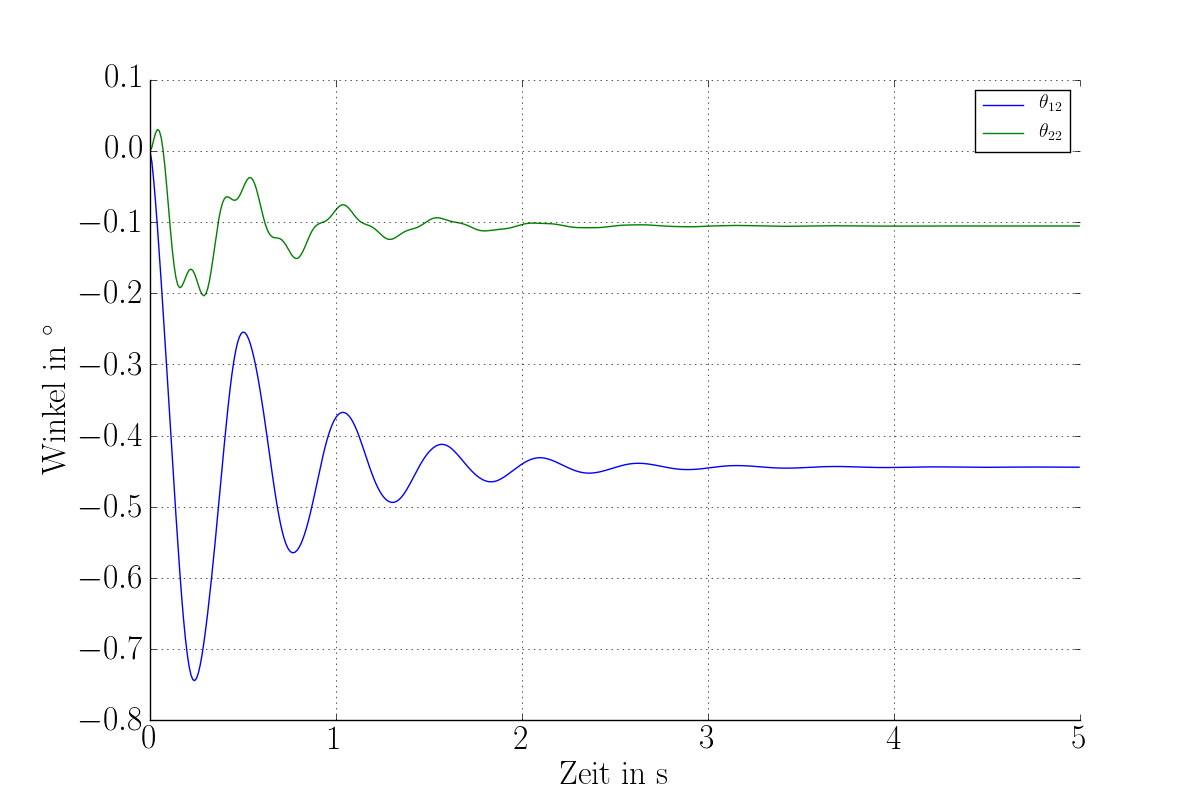
\includegraphics[width=1\linewidth]{RuhelageUnaktuierteGelenke.png}
\caption{Simulationsergebnisse unaktuierte Geleneke unvollständig aktuiertes Modell}
\label{fig:RuhelageUnaktuierteGelenke}
\end{figure}

In Abbildung \ref{fig:RuhelageUnaktuierteGelenke} ist der Winkelverlauf der unaktuierten Gelenke zu sehen. Zum Zeitpunkt $t=0$ haben diese Winkel keine Auslenkung. Innerhalb von zirka $3\,\si{s}$ schwingt sich der Ausleger in seine neue Ruhelage ein. Die Winkel sind negativ. Bei Betrachtung der Anordnung ist eine Durchbiegung, welche durch die zusätzlichen Gelenke modelliert ist, in mathematisch negative Richtung zu erwarten, da durch die Gravitationskraft ein Moment in der selben Richtung auf die Gelenke wirkt. Der Winkel $\theta_{12}$ hat eine größere Auslenkung, da der längere Teil des Auslegers durch seine höhere Masse ein stärkeres Moment ausübt.

\begin{figure}[h]
\centering
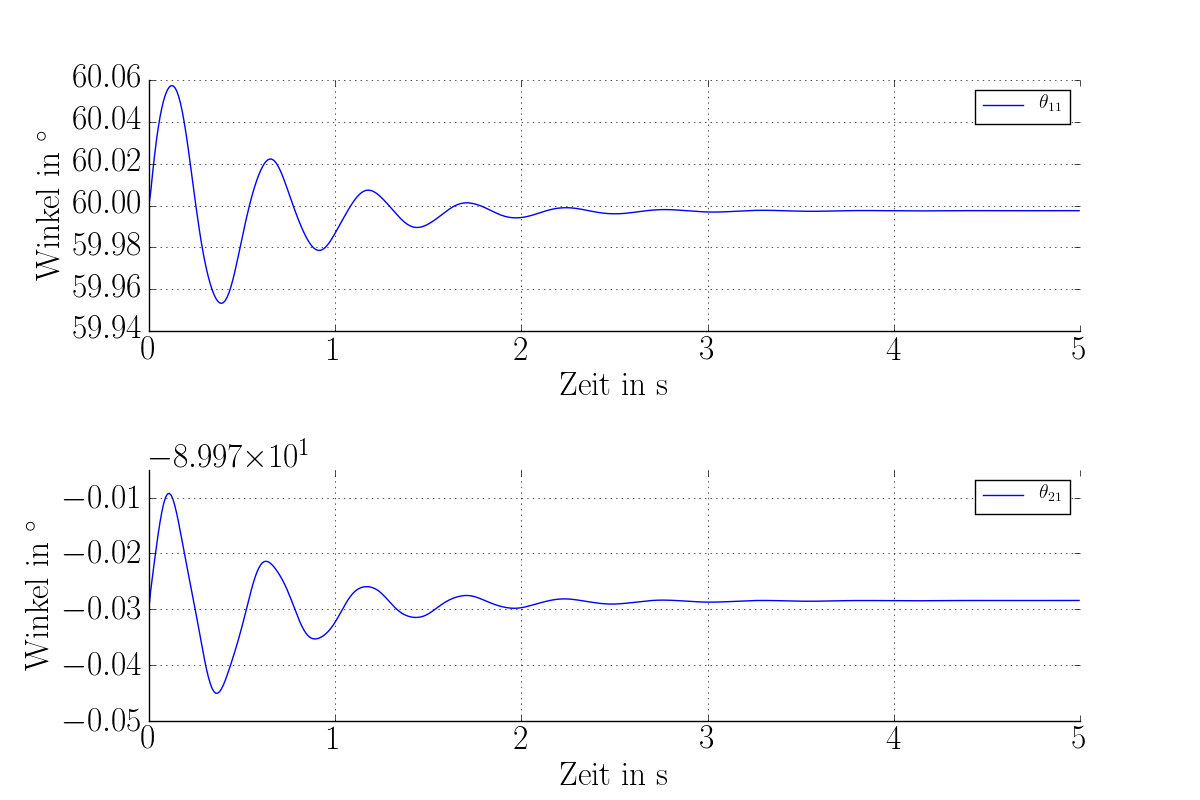
\includegraphics[width=1\linewidth]{RuhelageGelenkQ1Q2.png}
\caption{Simulationsergebnisse aktuierte Gelenke mit Einzelgelenkregelung}
\label{fig:RuhelageGelenkQ1Q2}
\end{figure}

Die Winkelverläufe der aktuierten Gelenke sind in Abbildung \ref{fig:RuhelageGelenkQ1Q2} gezeigt. Die Vorsteuerung kompensiert lediglich den Gravitationseinfluss, das heißt das Moment, welches dabei berechnet wird, ist über die gesamte Simulationsdauer konstant. Die Simulation startet nicht in der Ruhelage, für welche die Kompensation berechnet wurde. Damit entspricht dieser Wert auch nicht exakt dem notwendigen. Bei Beginn lenken die unaktuierten Gelenke im Uhrzeigersinn aus, wodurch ein leichter mathematisch positiver Ausschlag der aktuierten Gelenke verzeichnet wird. Die Regelung der einzelnen Gelenke wirkt dagegen. Nach dem Einschwingen verbleiben geringe stationäre Abweichungen, da nur ein PD-Regler verwendet wird, dessen Verstärkungen nicht optimal gewählt wurden. Die Simulationsergebnisse deuten an, dass die Einzelgelenkregelung in den Ruhelagen ausreichend ist, weil nur geringe Abweichungen auftreten.
 
\section{Modell der Regelung unvollständig aktuiert (3. Fall)}

In diesem Fall kann durch die Kenntnis des unvollständig aktuierten Modells eine Ruhelage exakt berechnet werden. 

In unserem Beispiel ergeben sich folgende Werte:

\begin{align*}
\theta_{11}^e&=60^\circ\\
\theta_{21}^e&=-90^\circ\\
\theta_{12}^e&=-0,679^\circ\\
\theta_{22}^e&=-0,124^\circ\\
\end{align*}

Die tatsächliche Ruhelage der unaktuierten Gelenke befinden sich dadurch in der berechneten, wodurch daraus keine Störmomente auf die aktuierten Gelenke ausgeübt werden.

\begin{figure}[h]
\centering
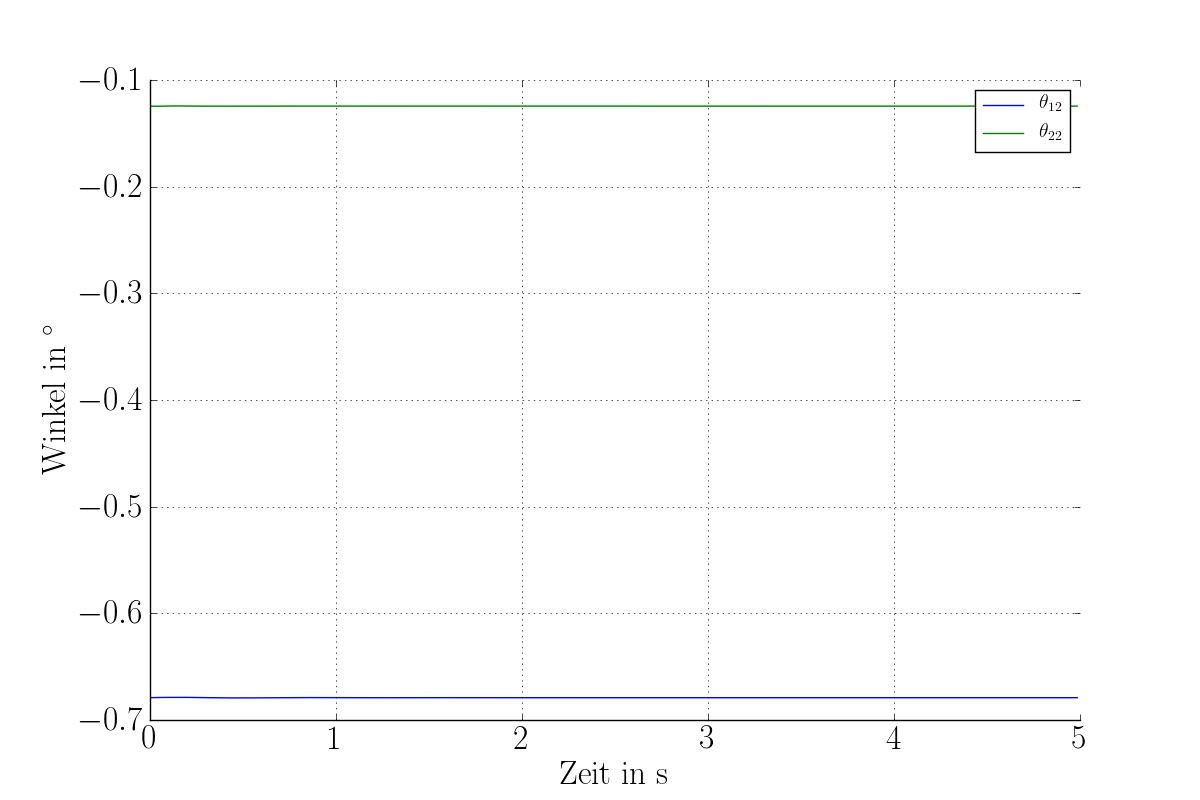
\includegraphics[width=1\linewidth]{lsgunvollvoll_unakt.png}
\caption{Simulationsergebisse unaktuierter Gelenke mit unvollständig aktuiertem Modell der Regelung}
\label{fig:unvollMod}
\end{figure}

Die Winkel $\theta_{12}$ und $\theta_{22}$ der unaktuierten Gelenke befinden sich sofort an der berechneten Position und sind konstant (Abbildung \ref{fig:unvollMod}). Dadurch treten sie nicht in Wechselwirkung mit den Winkeln der anderen Gelenken.

\begin{figure}[h]
\centering
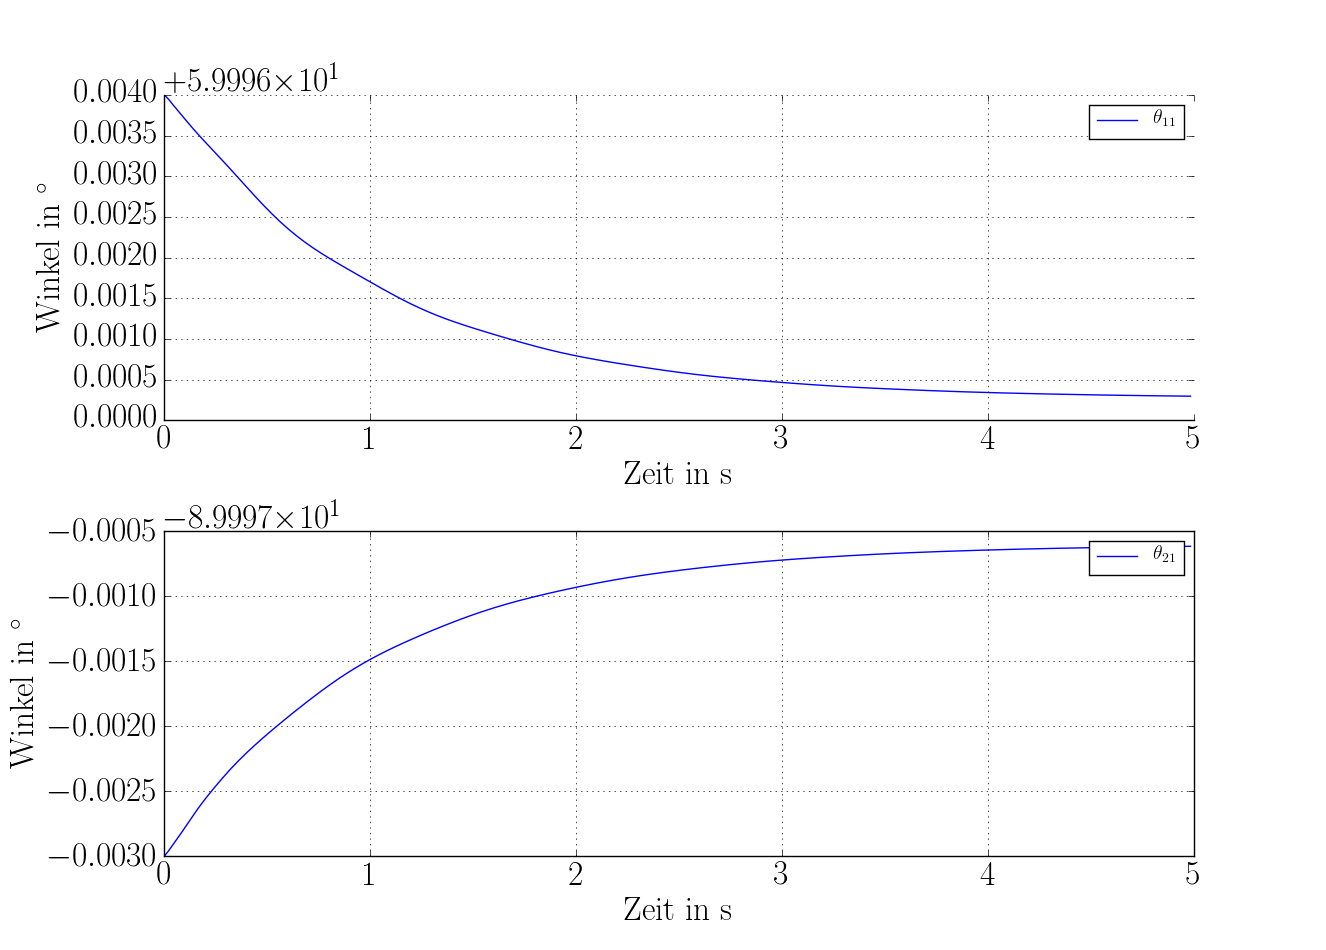
\includegraphics[width=1\linewidth]{lsgunvollvoll_akt.png}
\caption{Simulationsergebnisse der aktuierten Gelenke mit exakt berechneter Ruhelage}
\label{fig:lsgunvollvoll_unakt}
\end{figure}

Die Winkel $\theta_{11}$ und $\theta_{21}$ der aktuierten Gelenke erreichen ihre Sollposition nicht exakt, da die Steuerung noch das vollständig aktuierte Modell annimmt und die Stellgröße für die Ruhelage ungenau berechnet. Die stationäre Abweichung ist sehr gering und beträgt in diesem Beispiel zirka $0,0035^\circ$ (vgl. Abbildung \ref{fig:lsgunvollvoll_unakt}). Dieser Wert resultiert aus einer Simulation und ist in der  Praxis approximiert Null.

\newpage
\section{Alle Modelle unvollständig aktuiert (4. Fall)}

Bei der zusätzlichen Berücksichtigung eines unvollständigen Modells der Vorsteuerung ist die Kenntnis der Trajektorien aller Zustandskomponenten notwendig. Für eine Ruhelage sind diese mit akzeptablen Aufwand zu berechnen. Sofern ein Arbeitspunktübergang zwischen zwei Ruhelagen vollzogen werden soll, muss ein Randwertproblem gelöst werden. Die Lösung besteht aus Trajektorien, welche den Systemdifferentialgleichungen genügen und in gewünschtem Verhalten lösen. %Daraus ergibt sich beispielsweise, dass alle Winkel in der Ruhelage exakt dieser entsprechen.
\chapter{Modellierung der Last}
\label{abs:Lastmodellierung}

Im allgemeinen Betrieb einer mobilen Betonpumpe kann davon ausgegangen werden, dass durch den Vorgang des Pumpens von Beton eine Last wirkt. In diesem Kapitel wird eine Beschreibungsform der Last hergeleitet, damit eine Simulation berechnet werden kann.

\section{Ansatz}

\begin{figure}[h]
	\centering
	\input{Lastansatz.pdf_tex}
	\caption{Modellierungsannahme der Last}
	\label{fig:Manipulator_Last}
\end{figure}

Eine Betonpumpe pumpt den Beton impulsweise. Nach hinreichend langer Zeit ist die Rohrleitung vollständig mit Beton gefüllt. An jeder Stelle der Rohrleitung befindet sich über die gesamte Zeit eine konstante Masse. Zusätzlich kann man sich vorstellen, dass die Masse pro Bogenelement der Leitung auch als konstant betrachtet werden kann, da der Beton einer Art des Schiebens unterliegt. Dadurch ändern sich durch das Pumpen nur die Massenträgheitsmomente der Segmente des Auslegers. Am Ende des Auslegers befindet sich ein senkrecht hängender Schlauch, durch welchen sich der Beton zielgenau platzieren lässt. Durch die Reibung an der Schlauchwand ergibt sich ein Auswurfverhalten mit Tiefpasscharakter. Approximiert lässt sich eine sprungförmige Belastung annehmen, welche die schlimmste Form einer Belastung darstellt. 

In den Modellgleichungen wird die Last als Punktmasse modelliert. Dafür wird bei der Herleitung der Bewegungsgleichungen am Ende des letzten Segmentes eine Masse berücksichtigt, die einen Einfluss auf dessen Trägheitsmoment ausübt. Im Vergleich zu der Modellierung ohne Last kommt ein Term hinzu, der multiplikativ mit der Masse der Last verknüpft ist. In der Simulation kann dieser Wert in Abhängigkeit von der Zeit beeinflusst werden.  

\begin{figure}[h]
	\centering
	\input{Manipulatorunterakt_Last.pdf_tex}
	\caption{Modellierungsansatz der Last}
	\label{fig:Manipulator_Last}
\end{figure} 

\chapter{Visualisierungen} \label{ch:Visualisierung}

Diverse Daten - beispielsweise Simulationsergebnisse - erfordern eine geeignete Aufbereitung und ansprechende Darstellung. In diesen Darstellungen können Zusammenhänge zwischen verschiedenen abhängigen Größen gezeigt werden, oder mit anderen verglichen werden.
Bei dynamischen Systemen sind oft die Zeitverläufe der Systemgrößen von Interesse, die für Analysen in Diagrammen gezeigt werden können. Für einen Überblick über das Verhalten eines Systems bieten sich darüber hinaus Animationen an.

In dem folgenden Abschnitt werden einige Erläuterungen zu der Animation der mobilen Betonpumpe gegeben. Bei sämtlichen abgebildeten Diagrammen stehen alle notwendigen Anmerkungen an den entsprechenden Stellen, so dass hier nicht weiter darauf eingegangen wird.

\section{Animation}

\begin{figure}[h]
\centering
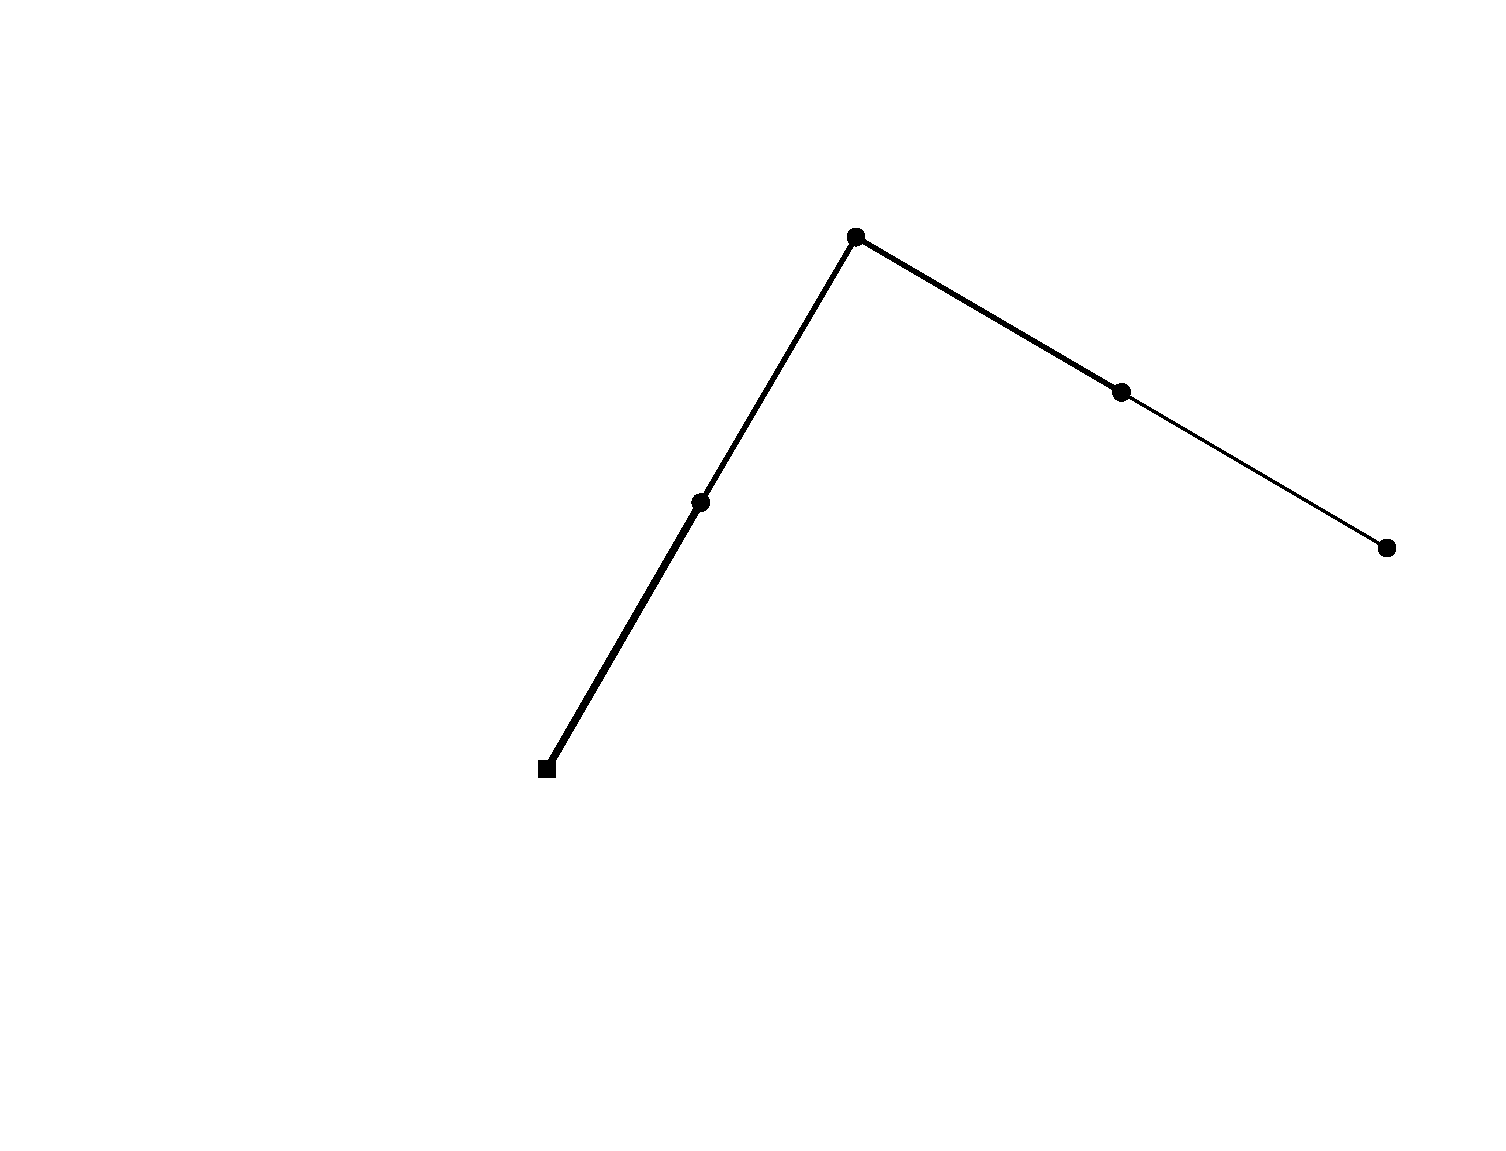
\includegraphics[width=0.7\linewidth]{animation01}
\caption[Animation Betonpumpe]{Animationsgrafik von 2 Gliedern (Auslegern) einer mobilen Betonpumpe}
\label{fig:animation}
\end{figure}

In der Abbildung \ref{fig:animation} sind zwei Glieder einer mobilen Betonpumpe mit zwei Auslegern abgebildet. Beide Träger wurden in der Modellbildung durch ein elastisches Knickgelenk in ihrer Mitte den realen Gegebenheiten angenähert. An dieser Stelle treten die unerwünschten Effekte auf, die es im Laufe des Seminars zu verringern gilt. 
\chapter{Zustandsstabilisierung}
\label{Zustandsstabilisierung}

In diesem Kapitel ist die Stabilisierung einer Ruhelage mithilfe der Zustandsrückführung beschrieben. \newline
Bisher wurde nur die Einzelgelenkregelung besprochen. Dabei hat die Regelabweichung eines Gelenkes nur Auswirkungen auf die Stellgröße des Selbigen. Die Matrix $\vect{K_{\mathrm{Regler}}}$ des Reglers hat nur Einträge auf der Diagonalen. Bei der im folgenden beschriebenen Zustandsrückführung kann jeder Zustand, bzw. jede Regelabweichung, die Stellgröße beeinflussen. Dabei ist die Matrix des Reglers theoretisch vollständig besetzt.  

\section{Berechnung der Zustandsrückführung}

Die Zustandsrückführung $\vect{F}$  kann auch als Regler aufgefasst werden, der die Strecke, d.h. das Modell der Betonpumpe, stabilisieren soll. Die Eingänge der Rückführung sind die Zustandsgrößen $\vect{\theta}$, $\vectd{\theta}$, die Winkel und Winkelgeschwindigkeiten der Gelenke und die Parameter der Ruhelage $\vect{\theta}^\mathrm{e}$. Die Stellgröße der Zustandsrückführung wird mit der Stellgröße der Vorsteuerung, wie in Abbildung \ref{fig:Blockdiagramm_Zustandsruckfuhrung} dargestellt, addiert und fungiert als Eingang der Strecke. Die Vorsteuerung berechnet aus dem Arbeitspunkt $\vect{\theta}^\mathrm{e}$, $\vectd{\theta}^\mathrm{e}$, $\vectdd{\theta}^\mathrm{e}$ die konstante Stellgröße zum Halten der Ruhelage. 

	\begin{figure}[h!]
		\centering
		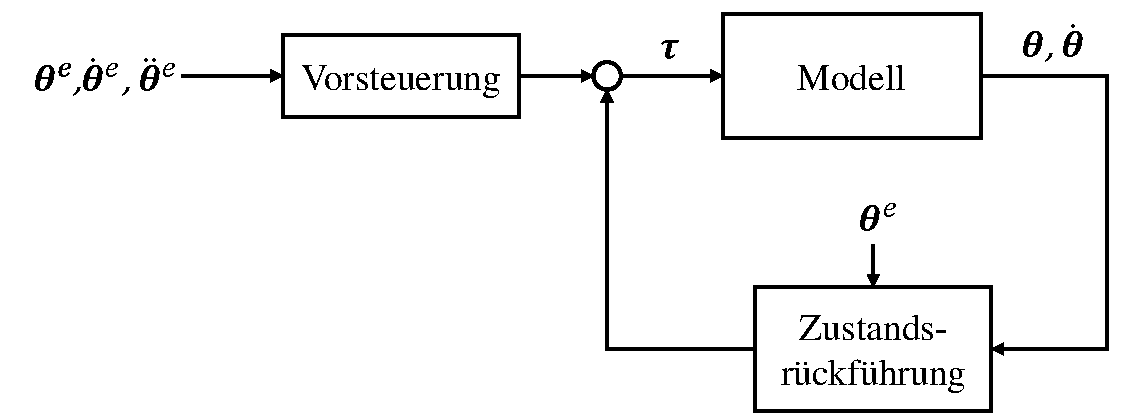
\includegraphics[scale=0.6]{Bilder/Zustansrueckfuehrung.pdf}
		\caption{Blockdiagramm der Zustandsrückführung}
		\label{fig:Blockdiagramm_Zustandsruckfuhrung}
	\end{figure}
	
Die Zustandsrückführung lässt sich aus der Systemmatrix $\vect{A}$, der Eingangsmatrix $\vect{B}$ und den gewünschten Eigenwerten  $\vect{\lambda}$ des Gesamtsystems, das bedeutet Strecke mit Rückführung, berechnen. Dies kann beispielsweise mit der Ackermannformel für Mehrgrößensysteme geschehen. Da das System dafür aufwendig in die Regelungsnormalform überführt werden muss, wird in dieser Arbeit die Rückführung lediglich mit einer bereits existierenden Matlab-Funktion "`place()"' berechnet. 
	
	\begin{equation}
		\vect{F} = \text{place}(\vect{A},\vect{B},\vect{\lambda})
	\end{equation}   	 

Dabei wird die Zustandsrückführung einmalig in Matlab berechnet und nach Python übertragen. Bei sich ständig ändernden Ruhelagen ist diese Vorgehensweise jedoch keine Lösung. Dafür sollte eine Berechnung in Python selbst bevorzugt werden. Zusätzlich kann nicht immer gewährleistet werden, dass die existierenden Algorithmen unter Python oder Matlab eine Lösung liefern. Sie sind abhängig von den gewünschten Eigenwerten, die im nächsten Abschnitt genauer erläutert werden. Es bietet sich daher an, bei veränderlichen Ruhelagen einen eigenen Algorithmus für die Berechnung zu entwickeln.

\section{Polvorgabe}
\label{abs:Polvorgabe}

Aus dem vorangegangen Abschnitt ist ersichtlich, dass die Pole des Gesamtsystems berechnet werden müssen. Sie beschreiben das Verhalten des Systems, welches sich aus der Strecke und der Zustandsrückführung zusammensetzt.\newline
Für den Vergleich werden zuerst die Pole des Systems mit der Einzelgelenkregelung berechnet. Die Eigenwerte des Gesamtsystems lassen sich aus $\vect{A} \in \mathbb{R}^{8\times8}$, $\vect{B} \in \mathbb{R}^{8\times2}$ und $\vect{K_{\mathrm{Regler}}} \in \mathbb{R}^{2\times8}$  mit der Python-Funktion "`np.linalg.eigvals()"' wie folgt berechnen:

	\begin{equation}
		\vect{\lambda} = \text{eig}(\vect{A} + \vect{B} \cdot \vect{K_{\mathrm{Regler}}})
	\end{equation} 

mit:

	\begin{equation*}
		\vect{K_{\mathrm{Regler}}} = \begin{pmatrix}
								3\cdot10^7 & 0 & 0 & 0 & 2\cdot10^7 & 0 & 0 & 0 \\ 
								0 & 0 & 6\cdot10^7 & 0 & 0 & 0 & 3\cdot10^7 & 0
							\end{pmatrix}. 
	\end{equation*} \newline

Es ergeben sich acht Pole, von denen sechs in dem Polplan in Abbildung \ref{fig:Polplan} als blaue Markierungen dargestellt sind. Alle Pole liegen auf der negativen reellen Halbebene. Das System ist somit stabil.  Der eine sichtbare Pol auf der reellen Achse hat eine Vielfachheit von zwei. Zwei der acht Pole sind rein reell mit einem sehr großen Betrag und daher in dem Diagramm nicht abgebildet. \newline
Ausgehend von der Einzelgelenkregelung werden, wie in Abbildung \ref{fig:Polplan} als grüne Markierungen dargestellt, die Pole der "`Polplatzierung 1"' gewählt. Die Beträge der Pole wurden verkleinert, um kleinere Stellsignale zu erhalten. Zusätzlich  wurde der Realteil der Pole, welche nahe an der imaginären Achse lagen, vergrößert. Bei Parameterschwankungen oder einer Regelung geringfügig außerhalb der Ruhelage können sich die Pole des Gesamtsystems verschieben. Liegen die Pole weiter links in der reellen negativen Halbebene kann die Stabilität somit auch bei größeren Schwankungen gewährleistet werden.\newline
Bei der "`Polplatzierung 2"', siehe Abbildung \ref{fig:Polplan} rote Markierungen, wurden sechs statt wie bisher vier der acht Pole konjugiert-komplex gewählt. Des Weiteren sind sie auf einem Kreisbogen um den Ursprung und mit betragsmäßig größerem Realteil angeordnet. Durch das zusätzliche konjugiert-komplexe Polpaar sollte sich die Dynamik des geschlossenen Systems erhöhen. \newline
	
	\begin{figure}[h!]
		\centering
		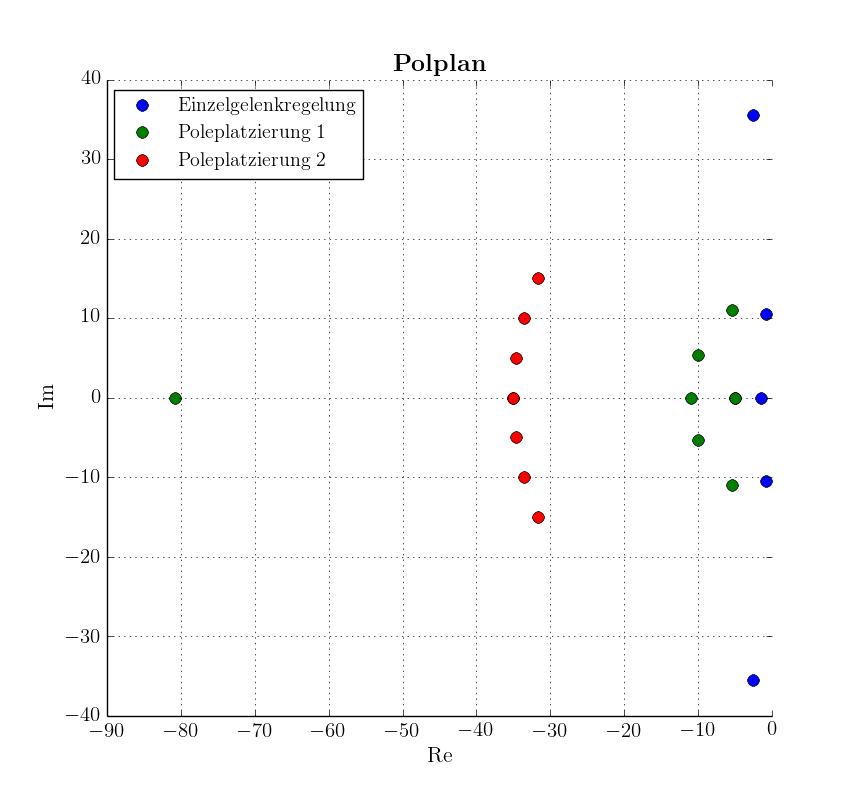
\includegraphics[scale=0.5]{Bilder/Pole.png}
		\caption{Polplan des geschlossenen Kreises}
		\label{fig:Polplan}
	\end{figure}
	
Da sich bei der Polvorgabe in diesem Abschnitt keine eindeutige Lösung finden lässt, sollen im Folgenden die einzelnen Regelungen bzw. Zustandsrückführungen miteinander verglichen werden.

\section{Simulationsergebnisse}

Für den Vergleich der einzelnen Rückführungen belastet man das nichtlineare Modell der Betonpumpe mit einer impulsweise konstanten Last. Diese Art der Belastung entspricht näherungsweise einem realen Pumpvorgang und wurde in Kapitel \ref{abs:Lastmodellierung} beschrieben. Dabei wird die Strecke alle zwei Sekunden für $0,5\,\si{s}$ mit einer zusätzlichen Masse von $100\,\si{kg}$ belastet. Dabei bewegen sich die Gelenke aus der Ruhelage. Die Regelung hat die Aufgabe das System  möglichst schnell, ohne bleibe Regelabweichung und mit geringen Überschwingen in die Ruhelage zu überführen. \newline
Je nach Anwendungsart der Betonpumpe ist die Einhaltung der drei Bedingungen unterschiedlich wichtig. Soll sie beispielsweise in engen und/ oder geschlossenen Räumen manövrieren, darf kein großes Überschwingen auftreten. Wird sie im Freien eingesetzt, spielt das Überschwingen keine große Rolle, hier sollte die Abweichung möglichst schnell ausgeregelt werden. \newline
Die Ergebnisse der Einzelgelenkregelung und der beiden Polplatzierungen aus \mbox{Abschnitt \ref{abs:Polvorgabe}} sind in den folgenden Diagrammen in Abbildung \ref{fig:Ergebnis_Zustandsruckfuhrung} dargestellt. Es sind jeweils die Winkel der aktuierten Gelenke  $\varphi_1 = \theta_{11}$, $\varphi_3 = \theta_{21}$ und die unaktuierten Gelenke $\varphi_2 = \theta_{12}$, $\varphi_4 = \theta_{22}$ über der Zeit $t$ abgebildet. Die Ruhelagen der aktuierten Gelenke betragen $\bar{\varphi}_1 = 60 \,^\circ$, $\bar{\varphi}_3 = -90\,^\circ$. Der Arbeitspunkt der unaktuierten Gelenke wird bei $\bar{\varphi}_2 = \bar{\varphi}_4 = 0 \,^\circ$ angenommen. Aufgrund der Durchbiegung weicht die tatsächliche von der angenommen Ruhelage ab.\newline
Aufgrund dieser Annahme berechnet die Vorsteuerung eine nicht ganz korrekte Stellgröße. Die Regelung versucht am Anfang der Simulation, zwischen $t\in[0;0,5]\,\si{s}$, die  Differenz zu kompensieren. Man erkennt, dass die Zustandsrückführung mit den sechs konjugiert-komplexen Eigenwerten (Polplatzierung 2) sehr schnell mit relativ großen Überschwingen reagiert. Der Stelleingriff an den aktuierten Gelenken hat auch einen Einfluss auf die Unaktuierten.   
    
	\begin{figure}[h!]
		\centering
		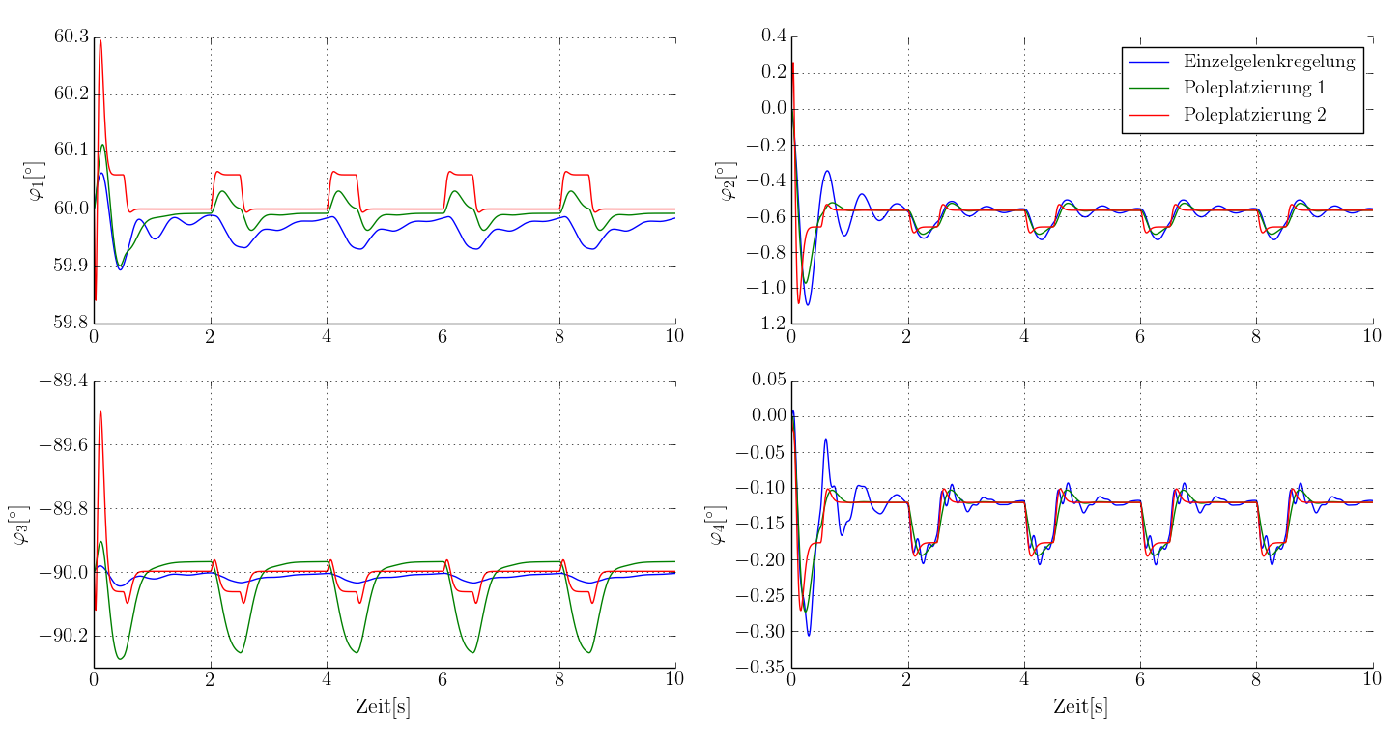
\includegraphics[scale=0.65]{Bilder/Ergebnissse_Zustandsrueckfuehrung.pdf}
		\caption{Verhalten der Zustandsrückführungen bei impulsweiser Belastung}
		\label{fig:Ergebnis_Zustandsruckfuhrung}
	\end{figure}

Die Einzelgelenkregelung schafft es nicht den Fehler der impulsweisen Belastung bei $\varphi_1$ innerhalb der 0,5 s auszuregeln. Auch nach der Entlastung wird der Winkel nur sehr langsam in die Ruhelage gebracht. Ein ähnliches Verhalten ist auch bei dem Gelenk  $\varphi_3$ zu beobachten. Die träge Regelung spiegelt sich auch bei den Winkelverläufen der unaktuierten Gelenke wieder. Bei dem Verlauf von $\varphi_4$ kann man die gewünschten unterschiedlichen Systemfrequenzen aus dem Abschnitt \ref{abs:Federparameter} beobachten.\newline
Die Zustandsrückführung der "`Polplatzierung 1"' in Abbildung \ref{fig:Ergebnis_Zustandsruckfuhrung} weist, wie zu erwarten, eine ähnliche Dynamik wie die Einzelgelenkregelung auf. Lediglich das Überschwingen ist bei $\varphi_1$ verringert. Die Regelung von Gelenk $\varphi_3$ ist dagegen um einiges schlechter. Hier tritt ein größeres Überschwingen bei bleibender Regelabweichung auf. \newline
Wie erwartet weist die Zustandsrückführung der "`Polplatzierung 2"' die größte Dynamik auf. Man erkennt in Abbildung \ref{fig:Ergebnis_Zustandsruckfuhrung}, bei dem Verlauf von $\varphi_1$, dass das System sehr schnell in einen Ruhepunkt überführt wird. Es tritt kaum Überschwingen auf. Während der Belastung wird das System jedoch um eine andere Ruhelage stabilisiert, d.h. es tritt eine bleibende Regelabweichung auf. Ein sehr ähnliches Verhalten zeigt sich auch bei der Regelung von Gelenk $\varphi_3$.\newline
Abschließend lässt sich sagen, dass die Zustandsrückführung der "`Polplatzierung 2"' die besten Ergebnisse liefert. Es würde sich anbieten die Realteile der Pole noch weiter zu erhöhen, um die bleibende Regelabweichung zu verringern. Auch die "`Polplatzierung 1"' liefert für das Gelenk $\varphi_1$ gute Ergebnisse. Es zeigt sich somit, dass bei gut gewählten Polen das System um einiges besser geregelt werden kann als mit der Einzelgelenkregelung. Lediglich das Einstellen der Pole benötigt Erfahrung um das Verhalten des Systems vorauszusagen. 

\chapter{Trajektorien-Folgeregelung}
Bis zu dem jetzigen Stand wurde die Betonpumpe lediglich um eine Ruhelage stabilisiert. Es ist jedoch zusätzlich notwendig den Ausleger der Betonpumpe von einem Arbeitspunkt in einen Anderen zu manövrieren. Die Planung, Steuerung und Regelung des Arbeitspunktwechsel soll im Folgenden näher beschrieben werden. 
\section{Trajektoriengenerierung}
Für den Arbeitspunktwechsel muss eine Trajektorie zwischen den Ruhelagen, im Gelenk\-raum, geplant werden. Diese soll für die Winkel, Winkelgeschwindigkeiten und -beschleuni\-gungen differentiell stetig und glatt sein. \newline
	\begin{figure}[h!]
		\centering
		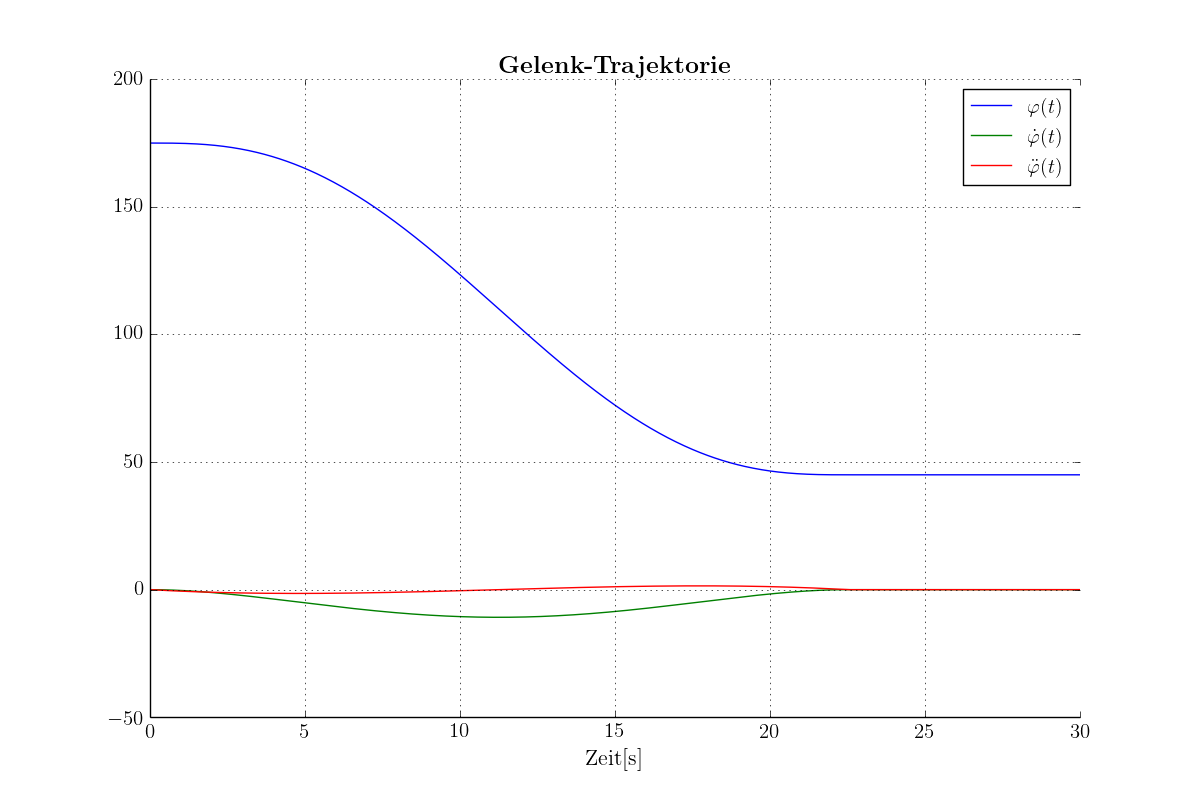
\includegraphics[scale=0.47]{Bilder/Trajektoriengenerierung.png}
		\caption{Beispieltrajektorie für den Arbeitspunktwechsel}
		\label{fig:Trajektoriengenerierung}
	\end{figure}\newline
Es wird ein Polynom vom Grad fünf für die Trajektorie angenommen. Durch Differentiation ergibt sich ein Polynomgrad von drei für die Winkelbeschleunigung. Ein solches Polynom ist stetig differenzierbar und differentiell glatt an den Anfangs- und Endwerten. Die sich daraus ergebenden sechs Unbekannten lassen sich aus den sechs Anfangs- und Endbedingungen und deren Zeiten berechnen. Die Winkelgeschwindigkeiten und -beschleunigungen sind in den Arbeitspunkten null. Die Winkel selbst sind von der Ausgangs- $(\varphi_a)$ und der Ziel- Ruhelage $(\varphi_e)$ abhängig.\newline
Für $\varphi_a= 180\,^\circ$, $\varphi_e= 45\,^\circ$ und einer Zeit $\Delta t=22\,\si{s}$ ergibt sich der in Abbildung \ref{fig:Trajektoriengenerierung} dargestellte Trajektorienverlauf.\newline	 
Da der Arbeitspunktwechsel im Gelenkraum geplant wird, kann wie oben beschrieben, eine separate Trajektorie für jedes Gelenk berechnet werden.\newline
In diesem Projekt wird dafür die bereits vorhandene Funktion "`trans\_poly"' der Bibliotheksklasse "`symb\_tools"' verwendet. Dabei werden wie oben beschrieben, die Anfangs- und Endbedingungen inkl. ihrer Zeitpunkte übergeben.\newline
Die beschriebene Planung der Trajektorie wird in den folgenden Abschnitten als Trajektoriengenerator zusammengefasst. Dieser berechnet zu diskreten Zeitpunkten für alle aktuierten Gelenke ihre Sollwinkel,-geschwindigkeiten und -beschleunigungen .  	
\section{Allgemeiner Aufbau}
Fügt man den neuen Block Trajektoriengenerator in den bereits existierenden Regelkreis mit Vorsteuerung und Einzelgelenkregelung, erhält man das Blockschaltbild aus Abbildung \ref{fig:Blockdiagramm_Trajektorien_Folgeregelung}. \newline
	\begin{figure}[h!]
		\centering
		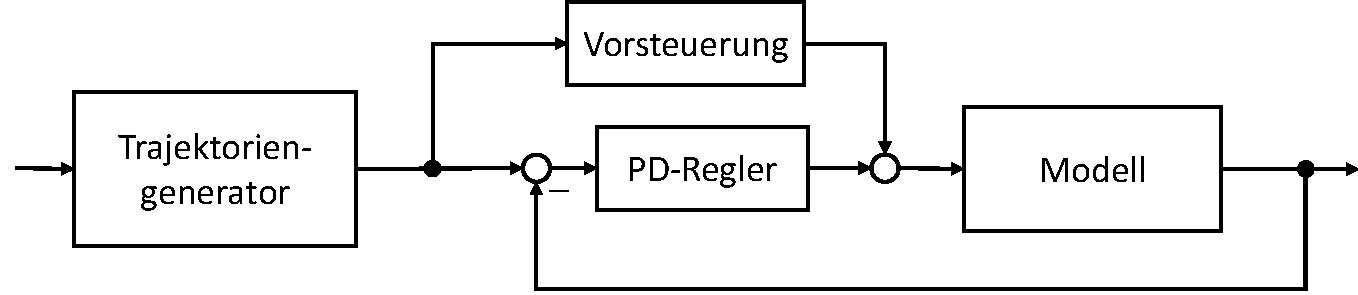
\includegraphics[scale=0.7]{Bilder/Blockdiagramm_Trajektorien_Folgeregelung.pdf}
		\caption{Blockdiagramm der Trajektorien-Folgeregelung}
		\label{fig:Blockdiagramm_Trajektorien_Folgeregelung}
	\end{figure}\newline 
Dabei wird aus dem aktuellen und dem neuen Arbeitspunkt eine Trajektorie berechnet. Zu den, für die Simulation notwendigen, Zeitpunkten werden diskrete Sollwerte für den Regelkreis generiert. Für ein besseres Führungsverhalten berechnet die Vorsteuerung aus den Sollwerten ($\varphi$, $\dot{\varphi}$, $\ddot{\varphi}$) Sollmomente für die Gelenke.\newline
Um den Einfluss von Störungen oder Modellunsicherheiten zu minimieren, wird eine PD-Einzelgelenkreglung hinzugefügt. Diese minimiert den Fehler zwischen dem Soll- und den Istverlauf der Strecke. \newline
Das Modell ist in der Realität die Betonpumpe selbst oder während der Simulation ein mathematisches Modell davon. 
\section{Reglereinstellung}
Bei einer exakten Vorsteuerung ist eine Regelung nicht notwendig, da jedoch das exakte Modell der Betonpumpe nicht abgebildet werden kann, kann auch keine exakte Vorsteuerung berechnet werden. So wird beispielsweise angenommen, dass die unaktuierten Gelenke einen konstanten Winkel von $\varphi = 0$ haben, in Wahrheit weichen sie um bis zu einigen Grad davon ab. Eine Regelung ist somit zwingend notwendig. \newline
Zusätzlich handelt es sich um ein hochgradig nichtlineares Modell. Bei der Verwendung der Zustandsstabilisierung aus Kapitel \ref{Zustandsstabilisierung} wäre die Linearisierung und somit die Systemmatrix abhängig von der Zeit, man erhält ein zeitvariantes System. Die Verwendung von nichtlinearen Regelungsansätzen ist ebenfalls kompliziert, da es sich um ein Mehrgrößensystem handelt und kein flacher Ausgang für das System gefunden wurde.\newline
Demzufolge soll in dieser Arbeit die Trajektorie mit einer einfachen PD-Reglung stabilisiert werden. Ein I-Anteil ist nicht notwendig, da die Stellgröße als Moment vorgegeben wird und die Sollgröße ein Winkel ist. Der offener Kreis besitzt somit bereits zwei Integratoren.\newline
	\begin{figure}[h!]
		\centering
		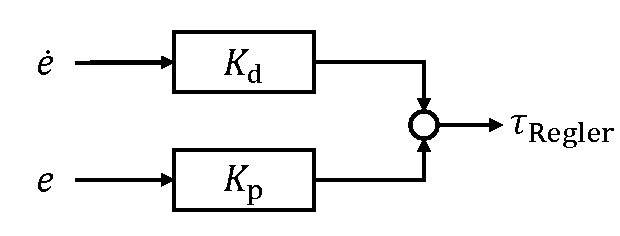
\includegraphics[scale=0.7]{Bilder/PD_Regler.pdf}
		\caption{Blockdiagramm der PD-Regelung}
		\label{fig:Blockdiagramm_PD_Regelung}
	\end{figure}\newline
Die PD-Regelung aus Abbildung \ref{fig:Blockdiagramm_PD_Regelung} wird als Einzelgelenkregler verwendet. In dieser Arbeit werden der Einfachheit halber nur Betonpumpen mit zwei aktuierten Gelenken untersucht. Es müssen somit vier Reglerparameter einzeln eingestellt werden.\newline
Die Parameter werden gleichmäßig erhöht, bis sich ein stabiles Verhalten mit hinreichend geringer Regelabweichung einstellt. Abhängig davon stellt man nun die Verstärkungen unabhängig voneinander ein, bis das gewünschte Verhalten erzielt wird. Dieses Vorgehen kann nur simulativ durchgeführt werden, um die Betonpumpe im Falle von instabilen Verhalten nicht zu beschädigen. Als Qualitätskriterium wird die Regelabweichung nach ca. zehn Sekunden verwendet, welche ungefähr der bleibenden Regelabweichung entspricht. Tabelle \ref{tab:Reglerparameter} zeigt die bleibende Regelabweichung für verschiedene Reglerparameter.\newline
	\begin{table}[h!]
	\caption{PD-Reglerparametrierung}
	\label{tab:Reglerparameter}
	\begin{tabular}{|c|c|c|c|c|c|c|}
		\hline \rule[-2ex]{0pt}{5.5ex}  Regler & $K_{\mathrm{p},1}\:\left[ \frac{\si{Nm}}{\si{rad}}\right]$ & $K_{\mathrm{d},1}\:\left[ \frac{\si{Nm}\cdot\si{s}}{\si{rad}}\right]$ & $K_{\mathrm{p},2}\si{ }\left[ \frac{\si{Nm}}{\si{rad}}\right]$ & $K_{\mathrm{d},2}\:\left[ \frac{\si{Nm}\cdot\si{s}}{\si{rad}}\right]$ & $e_{\varphi_1,\infty}\,^\circ$ & $e_{\varphi_3,\infty}\,^\circ$ \\ 
		\hline \rule[-2ex]{0pt}{5.5ex} $0$ & $1\cdot10^5$  & $1\cdot10^5$ & $1\cdot10^5$ & $1\cdot10^5$ & $-216,8$ & $-60,34$ \\
		\hline \rule[-2ex]{0pt}{5.5ex} $1$ & $1\cdot10^6$  & $1\cdot10^6$ & $1\cdot10^6$ & $1\cdot10^6$ & $6,854\cdot10^{-2}$ & $-1,226\cdot10^{-1}$ \\
		\hline \rule[-2ex]{0pt}{5.5ex} $2$ & $1\cdot10^7$  & $1\cdot10^7$ & $1\cdot10^7$ & $1\cdot10^7$ & $5,467\cdot10^{-3}$ & $-1,248\cdot10^{-2}$ \\
		\hline \rule[-2ex]{0pt}{5.5ex} $3$ & $3\cdot10^7$  & $2\cdot10^7$ & $6\cdot10^7$ & $3\cdot10^7$ & $1,783\cdot10^{-3}$ & $-2,087\cdot10^{-3}$ \\
		\hline 
	\end{tabular} 
	\end{table}
Man erkennt, dass bei zu geringen Verstärkungen (Regler 0) das System instabiles Verhalten aufweist. Erhöht man die Parameter um eine Potenz (Regler 1) stabilisiert der Regler die Strecke. Nun werden die Parameter solange angepasst, bis sich eine Genauigkeit von einigen tausendstel Grad einstellt. Es ergibt sich die Reglerparameterkonstellation drei.\newline
Es ist ersichtlich, dass trotz der zwei Integratoren der Strecke die bleibe Regelabweichung nicht auf Null geregelt werden kann. Eine Genauigkeit von wenigen tausendstel Grad ist jedoch für den Betrieb einer Betonpumpe mehr als ausreichend.
\section{Simulationsergebnisse}
Eine typische Bewegung der Betonpumpe ist in Abbildung \ref{fig:Verlauf_Trajektorienfolgeregelung} dargestellt. Dabei werden die Glieder aus einer Transportposition (alle Glieder sind auf dem Transportfahrzeug eingeklappt, siehe linker Teil) in eine Arbeitsposition (siehe rechter Teil) verfahren. Die in dem Diagramm in Abbildung \ref{fig:Verlauf_Trajektorienfolgeregelung} gezeigten Gelenkverläufe sind die simulierten Verläufe. 
	\begin{figure}[h!]
		\centering
		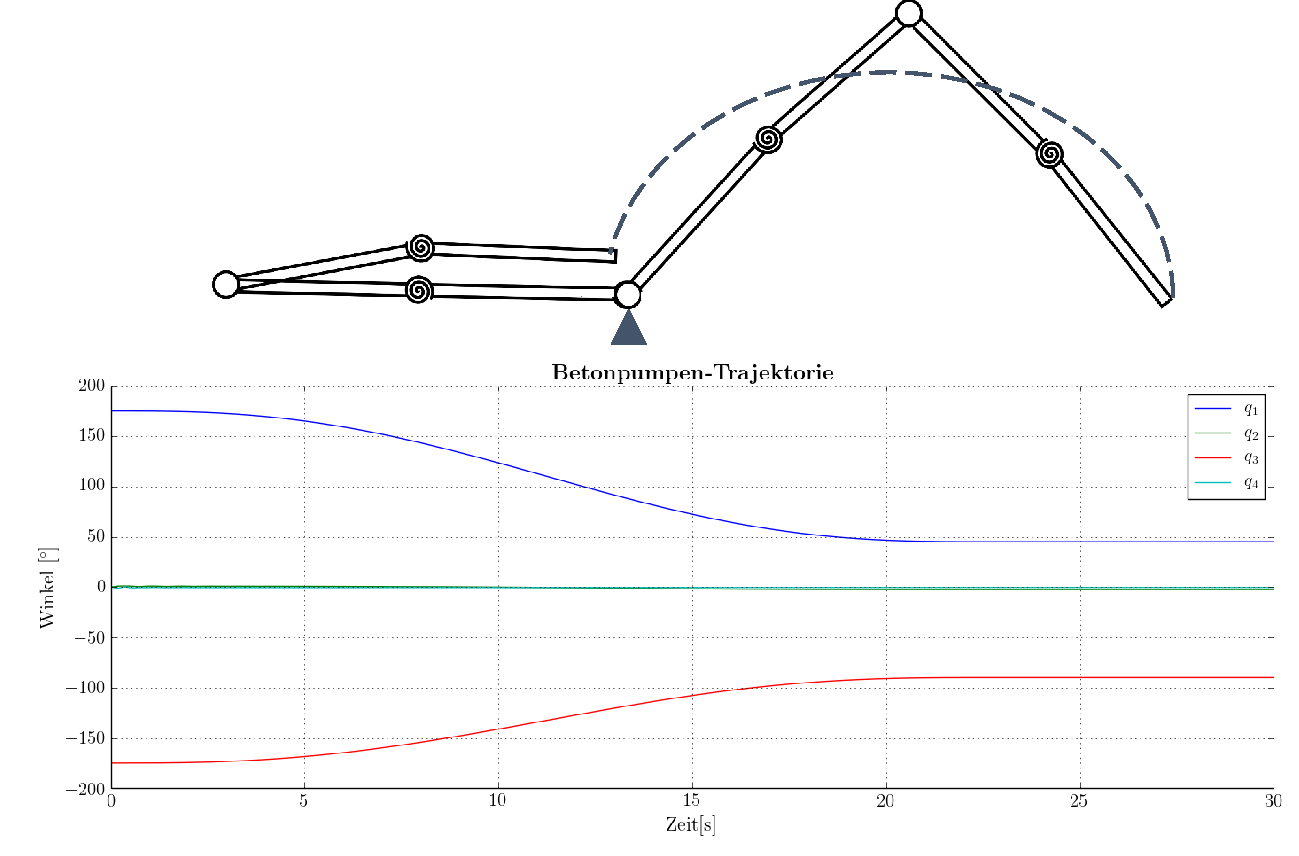
\includegraphics[scale=0.7]{Bilder/Verlauf_Trajektorienfolgeregelung.pdf}
		\caption{Gelenktrajektorien mit Folgeregelung}
		\label{fig:Verlauf_Trajektorienfolgeregelung}
	\end{figure}\newline
Stellt man die Regelabweichungen während der Bewegung der Gelenke $\varphi_1$  und $\varphi_3$ über die Zeit dar, erhält man das Diagramm in Abbildung \ref{fig:Regelabweichung_Folgeregelung}. Die bleibenden Abweichungen aus Tabelle \ref{tab:Reglerparameter} entsprechen den Regelabweichungen bei $t=30\,\si{s}$. Man erkennt, dass die Differenz aus Soll- und Istwinkeln in der Transportposition ($t=3\,\si{s}$) bedeutend kleiner als in der Arbeitsposition ($t=30\,\si{s}$) ist.
\newline 
	\begin{figure}[h!]
		\centering
		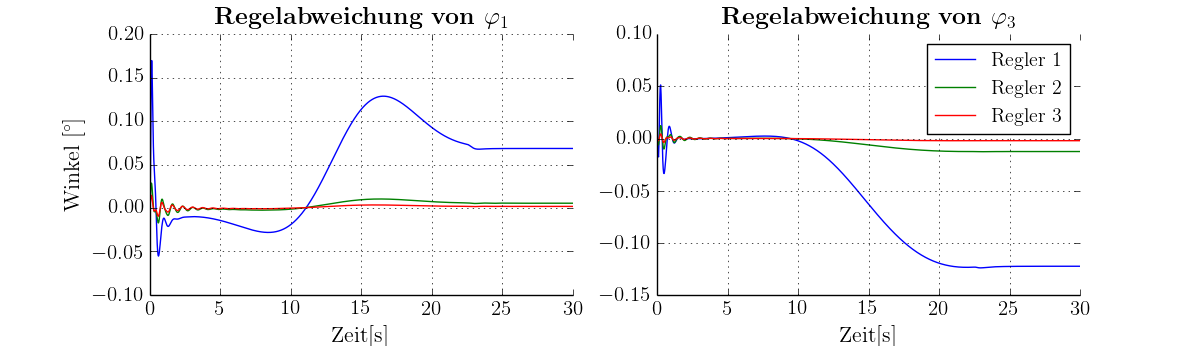
\includegraphics[scale=0.55]{Bilder/Regelabweichung_Folgeregelung.png}
		\caption{Regelabweichung der Trajektorien-Folgeregelung für $\varphi_1$, $\varphi_3$}
		\label{fig:Regelabweichung_Folgeregelung}
	\end{figure}\newline
	
\section{Stellgrößenabschätzung}
Theoretisch wäre es möglich die bleibende Regelabweichungen durch sehr große Verstärkungen immer weiter zu minimieren. Die Stellgrößen hängen jedoch direkt von den Reglerparametern und der Vorsteuerung ab. Daher bietet es sich an im Folgenden eine maximale Schranke für die Stellgrößen zu schätzen. \newline
Für die obere Grenze soll die Betonpumpe vollständig ausgestreckt mit ihrer kompletten Masse am äußersten Punkt belastet werden. Abbildung \ref{fig:Stellgroessenabschaetzung} zeigt diese Anordnung für die in der Arbeit diskutierten Betonpumpe mit jeweils zwei aktuierten und unaktuierten Gelenken.   
\newline
	\begin{figure}[h!]
		\centering
		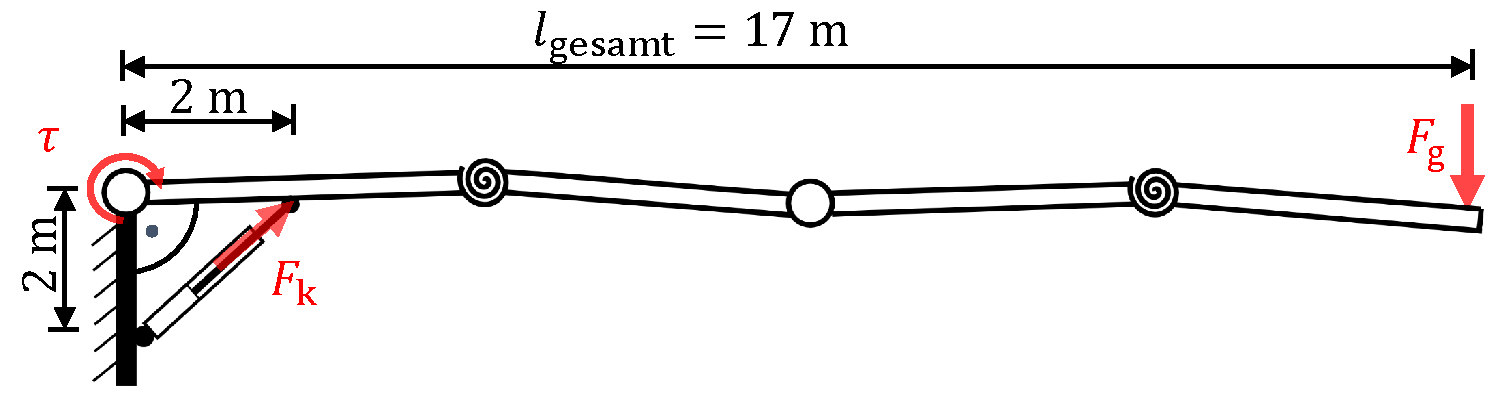
\includegraphics[scale=0.6]{Bilder/Stelgroessenabschaetzung.pdf}
		\caption{Abschätzung der maximalen Stellgrößen}
		\label{fig:Stellgroessenabschaetzung}
	\end{figure}\newline
Durch eine Belastung von $m_{\mathrm{gesamt}} = 4250\,\si{kg}$ ergibt sich ein Moment $\tau_g$ von:
	\begin{equation}
		\tau_g = l_{\mathrm{gesamt}}\cdot g\cdot m_{\mathrm{gesmat}}\approx 700 \,\si{kNm}.
	\end{equation}  
Bei der Verwendung eines trivial angeordneten Hydraulikzylinders, wie in Abbildung \ref{fig:Stellgroessenabschaetzung}, muss eine Kraft $F_k$ aufgebracht werden, um das Moment $\tau_g$ zu kompensieren.  Es gilt:
	\begin{equation}
		\tau = \tau_k-\tau_g = 0 \,\si{Nm}.
	\end{equation}
Somit ergibt sich $F_k$ zu
	\begin{equation}
		F_k = \sqrt{2}\cdot \frac{\tau_k}{2\,\si{m}} \approx 500\,\si{kN}.
	\end{equation}

Recherchen zeigen, dass Kräfte von mehr als $500\,\si{kN}$ mit Hydraulikzylindern realisiert werden können. Aus Sicherheitsgründen wird die Kraft etwas erhöht und eine maximale Stellgröße von $\tau_{k,\mathrm{max}} = 1 \,\si{MNm}$ verwendet. Während der Simulation werden alle Stellgrößen auf diesen Wert beschränkt.\newline
\newline
	\begin{figure}[h!]
		\centering
		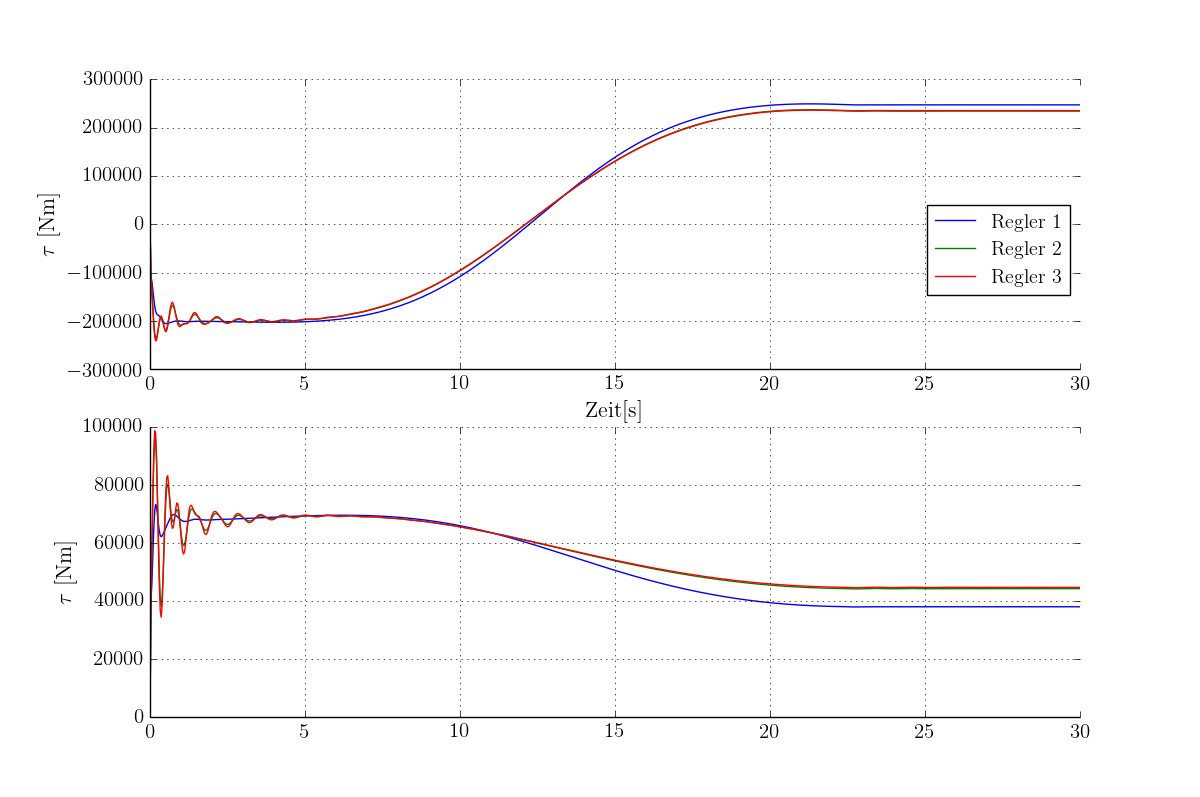
\includegraphics[scale=0.5]{Bilder/Stellgroessen_Trajektorien_Folgeregelung.png}
		\caption{Stellgrößenverlauf der Trajektorien-Folgeregelung}
		\label{fig:Stellgroessen_Trajektorien_Folgeregelung}
	\end{figure}\newline
Der Stellgrößenverlauf der Trajektorien-Folgeregelung ist in Abbildung \ref{fig:Stellgroessen_Trajektorien_Folgeregelung} dargestellt. Man erkennt, dass die maximale Stellgröße von $\tau_{k,\mathrm{max}} = 1 \,\si{MNm}$ weit unterschritten wird. Die Bewegung kann somit von einer realen Betonpumpe durchgeführt werden. 

\section{Einführung von Modellungenauigkeiten}
Aus Abbildung \ref{fig:Stellgroessen_Trajektorien_Folgeregelung} ist ersichtlich, dass die Regelung nach der Einschwingphase, ab $t=5\,\si{s}$ kaum dynamische Stellgrößen generiert. Es zeigt sich, dass die Vorsteuerung sehr gut dem inversen Streckenmodell entspricht. Bei einer realen Betonpumpe wird dies nicht mehr der Fall sein. Um dennoch Stabilität und ein gutes Führungsverhalten gewährleisten zu können, werden nachfolgend Modellungenauigkeiten eingefügt, die nicht in der Vorsteuerung betrachtet werden.\newline
	\begin{figure}[h!]
		\centering
		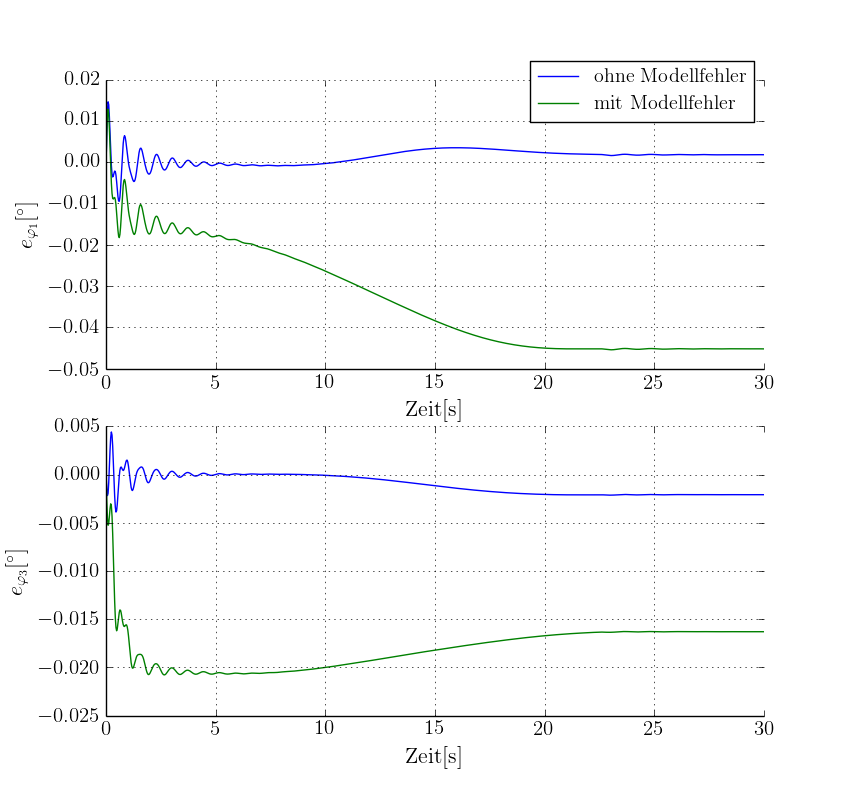
\includegraphics[scale=0.5]{Bilder/Modellungenauigkeiten.png}
		\caption{Regelabweichung mit Modellungenauigkeiten}
		\label{fig:Regelabweichung_Modellungenauigkeiten}
	\end{figure}\newline
Dabei wird der Wert aller Modellparameter für die Simulation um $\pm20 \,\%$ variiert. Abbildung \ref{fig:Regelabweichung_Modellungenauigkeiten} zeigt den Verlauf der Regelabweichung während der Bewegung. Es ist ersichtlich, dass das System trotz der Ungenauigkeiten stabilisiert werden kann. Lediglich die Regelabweichungen sind um einiges größer. Da es sich bei den Ungenauigkeiten um eine zufällige Verteilung handelt werden fünf Messungen durchgeführt und die stationären Regelabweichungen gemittelt. Die ermittelten Werte von \mbox{$e_{\varphi_1,\infty}=4,508\cdot10^{-2}\,^\circ$} und $e_{\varphi_3,\infty} = 5,368\cdot10^{-3}\,^\circ$  liegen jedoch immer noch weit unter den für den Betrieb einer Betonpumpe notwendigen Abweichungen. Diese ersten Versuche zeigen, dass die Trajektorien-Folgeregelung durchaus auch bei einer realen Betonpumpe mit zwei Armsegmenten angewendet werden kann. 

\chapter{Zusammenfassung und Ausblick}
Die hier angefertigte Arbeit ist Teil des Oberseminars der Regelungs- und Steuerungstheorie. Ziel des Seminars war die Untersuchung, Steuerung und Regelung eines Auslegers einer mobilen Betonpumpe. Die Arbeit wurde in einer Gruppe von drei Studenten durchgeführt. Im folgenden Abschnitt werden die Ergebnisse noch einmal zusammengefasst dargestellt und ein Ausblick für das mögliche weitere Vorgehen gegeben
  
\section{Zusammenfassung der Ergebnisse}
Einen großen zeitlichen Aufwand stellte die Darstellung des Verhaltens der Ausleger der Betonpumpe als mathematische Gleichungen dar. Diese Modellierung wurde mit konzentrierten Parametern durchgeführt. Um das dynamische Verhalten und die Durchbiegung gut darstellen zu können, wurde pro Armsegment ein passives unaktuiertes Zusatzgelenk betrachtet. Diese Modellierung war die Voraussetzung für alle weiteren Schritte.\newline
Um das Systemverhalten der Betonpumpe abzubilden, wurden sämtliche Parameter der Modellierung unter Verwendung von realen Daten berechnet. \newline
Zusätzlich wurde das erhaltene Systemmodell linearisiert und in die Zustandsdarstellung überführt. Dadurch war es möglich einen Nachweis der Stabilität in der Ruhelage zu erbringen und eine Zustandsrückführung zu berechnen.\newline
Es wurden verschiedene Varianten diskutiert, wie viele Modellinformationen für die Regelung und Steuerung einbezogen werden sollen. Dadurch konnten ihre Auswirkungen auf das Verhalten der Betonpumpe in mehreren Simulationen untersucht werden.\newline
Es wurde eine impulsweise Belastung eingeführt, die die reale Belastung gut approximiert. Dadurch war es möglich verschiedene Regelungskonzepte miteinander zu vergleichen.\newline
Diese Regelungskonzepte sind u.a. die Einzelgelenkregelung, wo jedes Gelenk unabhängig von den anderen mit einem PD-Regler stabilisiert wird. Als eine weitere Möglichkeit für die Ruhelagenstabilisierung wurde die Zustandsrückführung vorgestellt. Dafür wurden die gewünschten Eigenwerte des Gesamtsystems vorgegeben, um eine Rückführung zu berechnen.\newline
Des Weiteren wurden Trajektorien im Gelenkraum geplant, um den Ausleger der Betonpumpe in eine neue Ruhelage überführen zu können. Die Stabilisierung während der Bewegung übernimmt eine Trajektorien-Folgeregelung. Für ein gutes Verhalten wurden die Parameter der Regelung gezielt eingestellt.\newline 
Letztendlich können durch die Einführung von Modellungenauigkeiten die genannten Konzepte der Regelung und Steuerung auch mit fehlerhaften Systemmodellen getestet werden. Dadurch ist es möglich ihr Verhalten bei einer realen Anwendung besser abschätzen zu können.
\section{Ausblick für weiteres Vorgehen}

Die Zusammenfassung in dem vorherigen Abschnitt zeigt, dass viele verschiedene Möglichkeiten der Modellierung, Regelung und Steuerung des Auslegers einer mobilen Betonpumpe untersucht wurden. Trotzdem konnten im Umfang des Oberseminars nicht alle möglichen Konzepte behandelt werden. \newline
So wurden bisher nur lineare Regelungskonzepte implementiert. Die Kenntnisse über Nichtlinearitäten konnten dabei leider nicht verwendet werden. Eine andere Möglichkeit ist die Eingang-Ausgang-Linearisierung. Dabei wird das vorhandene nichtlineare Modell partiell linearisiert, indem ein neuer Eingang eingeführt wird. Die neue Stellgröße ist die Winkelbeschleunigung. Bisher wurde das Moment als Eingang benutzt. Das daraus entstandene partiell lineare System kann mit den Methoden der linearen Regelungstechnik stabilisiert werden. \newline
Des Weiteren kann eine Trajektorienplanung für die unaktuierten Gelenke entwickelt werden. Da diese Gelenke nicht aktiv gesteuert werden können, beschreibt die Trajektorie nur die Bewegung, die durch die Steuerung der aktuierten Gelenke verursacht wird. Dadurch kann der gesamte Ausleger auf einer gezielten Trajektorie in Gelenk- und Arbeitsraum (Raumkoordinaten und Orientierung) bewegt werden. Bei dieser Aufgabe wird  eine Randwertaufgabe gelöst.\newline
In dieser Arbeit wurden bisher alle Untersuchungen lediglich an einem Ausleger mit zwei aktuierten Gelenken vorgenommen. In der Einleitung erkennt man, dass eine reale Betonpumpe mehr als fünf aktive Gelenke besitzen kann. Es sollten daher die in der Arbeit vorgestellten Konzepte der Regelung und Steuerung auf eine solche Anzahl übertragen werden. Dabei entstehen sehr große Gleichungssysteme, die ein symbolisches Lösen nahezu unmöglich machen.\newline
Trotz der genannten unbearbeiteten Aufgaben bieten die in dieser Arbeit gezeigten Ergebnisse eine gute Grundlage für die tatsächliche Regelung und Steuerung einer mobilen Betonpumpe.

%
%\chapter{Erläuterungen zur Klasse ArbeitRST}
In den folgenden Abschnitten werden einige Erläuterungen zur \LaTeX-Dokumentenklasse \texttt{ArbeitRST.cls} gegeben werden. Diese basiert auf der Klasse \texttt{scrbook} aus dem KOMA-Script-Paket und kann daher mit Hilfe der Methoden aus diesem Paket modifiziert werden. Für nähere Informationen dazu sei auf die KOMA-Script-Anleitung\footnote{Diese kann unter der URL \url{http://www.ctan.org/pkg/koma-script} heruntergeladen werden.} und die Website
\begin{center}
	\url{http://www.komascript.de/}
\end{center}
verwiesen. 

Die wesentlichsten Änderungen gegenüber der ursprünglichen Klasse bestehen in einer angepassten Titelseite und der hinzugefügten Selbstständigkeitserklärung.
\section{Informationen zu schriftlichen Arbeiten am RST}
Informieren Sie sich in der für Sie relevanten Prüfungsordnung über die \emph{Anzahl der geforderten Exemplare} die eingereicht werden müssen. Bitte beachten Sie, dass jedes dieser Exemplar die \emph{Aufgabenstellung} enthalten muss. Lassen Sie diese bitte beim Binden zwischen der Titelseite und der Selbstständigkeitserklärung einfügen. Eines der Exemplare muss dabei das \emph{originale}, vom Vorsitzenden des Prüfungsausschusses und dem verantwortlichen Hochschullehrer unterzeichnete, Dokument enthalten, bei den restlichen genügen Kopien. Bitte beachten Sie, dass die Arbeit \emph{einseitig} ausgedruckt werden muss. Ausschlaggebend für die fristgemäße Einreichung ist die \emph{Bestätigung des Prüfungsamtes}. Informieren Sie sich daher im \emph{Vorfeld} über die Öffnungszeiten am Abgabetag. Sollte das Prüfungsamt geschlossen haben, ist es in der Regel möglich mit den Mitarbeitern eine individuelle Vereinbarung zu treffen.
\section{Die Titelseite}
Die Titelseite kann über die in Tabelle \ref{tab:titel} angegebenen Befehle angepasst werden.
\begin{table}[htbp]
\caption{Befehle zum Anpassen der Titelseite}
\label{tab:titel}
\begin{tabular}{lp{12cm}}
Befehl & Bedeutung\\
\toprule
\verb|\author| & legt den Namen des Autors der Arbeit fest\\
\verb|\geburtsdatum| & legt das Geburtsdatum des Autors fest\\
\verb|\geburtsort| & legt das Geburtsort des Autors fest\\
\verb|\title| & legt den Titel der Arbeit fest\\
\verb|\subtitle| & legt den Untertitel der Arbeit fest\\
\verb|\betreuer| & fügt einen Betreuer hinzu\\
\verb|\date| & legt das Einreichungsdatum der Arbeit fest -- \newline wird dieser Befehl nicht aufgerufen wird standardmäßig das zum Kompilationszeitpunkt eingestellte Systemdatum verwendet.\\
\bottomrule
\end{tabular}
\end{table}
\section{Die Selbstständigkeitserklärung}
In der Selbstständigkeitserklärung werden automatisch der Typ der Arbeit, ihr Titel sowie der Name des Autors übernommen. Der Ort kann über den Befehl \verb|\selbstort| geändert werden, wobei standardmäßig "`Dresden"' verwendet wird. Das Datum ist standardmäßig identisch zum Einreichungsdatum, kann aber mit dem Befehl \verb|\selbstdatum| geändert werden.

\section{Kurzfassung}
Eine Kurzfassung der Arbeit kann mit dem Befehl \verb|\kurzfassung{deutsch}{englisch}| eingefügt werden. Das erste Argument entspricht dabei der deutschen, das zweite der englischen Version.

\section{Auswahl des Typs der Arbeit}
Zur Auswahl des Typs der Arbeit steht die Klassenoption \texttt{arbeit} zur Verfügung. Mit dieser können sie zwischen Diplom-, Master- und Studienarbeit sowie dem Bericht zum Forschungspraktikum auswählen:
\begin{table}[hbtp]%
\caption{Auswahl des Typs der Arbeit mittels Klassenoptionen}
\centering
\begin{tabular}{cc}
Diplomarbeit & \verb|\documentclass[arbeit=diplom]{ArbeitRST}|\\
Masterarbeit & \verb|\documentclass[arbeit=master]{ArbeitRST}|\\
Studienarbeit & \verb|\documentclass[arbeit=studie]{ArbeitRST}|\\
Bericht zum Forschungspraktikum & \verb|\documentclass[arbeit=forsch]{ArbeitRST}|
\end{tabular}
\label{}
\end{table}

\section{Eingebundene Pakete}
In der Dokumentenklasse werden bereits einige \LaTeX-Pakete geladenen. Davon sind die zum Verfassen einer Arbeit möglicherweise relevanten in der Tabelle \ref{tab:pakete} aufgeführt. 
\begin{table}[htbp]%
\centering
\caption{Auswahl eingebundener Pakete}
\label{tab:pakete}
\begin{tabular}{p{3.6cm}p{11.4cm}}
amsmath, amssymb, \newline amsfonts, amsthm & Pakete zum Satz mathematischer Formeln, Dokumentation finden sie unter \newline\url{http://www.ams.org/publications/authors/tex/amslatex},\newline besonders empfehlenswert ist der "`Short Math Guide for \LaTeX"'\\
booktabs & ermöglicht das Setzen "`schöner"' Tabellen, Dokumentation unter \url{http://ctan.org/pkg/booktabs}\\
cite & verbessert einige Aspekte des Zitierens, Dokumentation unter \newline\url{http://ctan.org/pkg/cite}\\
caption, subcaption & Pakete zum Anpassen der Unter- und Überschriften von Tabellen, Grafiken etc., Dokumentation unter \newline\url{http://ctan.org/pkg/caption} \newline\url{http://ctan.org/pkg/subcaption}
\end{tabular}
\end{table}\\
Neben diesen Paketen wird das Paket \verb|hyperref| (\url{http://ctan.org/pkg/hyperref}) zur farbigen Hervorhebung von Verweisen, Links etc.\ eingebunden. Bitte deaktivieren Sie diese Markierungen vor dem Ausdrucken mit Hilfe des Befehls
\begin{center}
\verb|\hypersetup{hidelinks}|.
\end{center}

\section{Zusätzliche Makros}
In die Dokumentenklasse \texttt{ArbeitRST} wurden einige Makros aufgenommen, die sich bei der Arbeit mit \LaTeX{} als nützlich erwiesen haben.
\begin{table}[htbp]
\centering
\caption{Zusätzliche Makros und Umgebungen}
\begin{tabular}{ccp{9cm}}
Syntax & Ausgabe & Beschreibung\\
\toprule
\texttt{\textbackslash vect\{a\}} & $\vect{a}$ & Umschaltung auf fette Schriftart im Mathemodus-- oft für Vektoren genutzt\\[2ex]
\texttt{\textbackslash diag(a,\textbackslash ldots,z)} & $\diag(a,\ldots,z)$ & Nützlich zur Definition von Diagonalmatrizen\\[2ex]
\texttt{\textbackslash diff[n]\{q\}\{t\}} & $\diff[n]{q}{t}$ & Ableitungen darstellen\\[2ex]
\texttt{\textbackslash partiell[n]\{q\}\{t\}} & $\partiell[n]{q}{t}$ & partielle Ableitungen darstellen\\[2ex]
\texttt{\textbackslash Reals} & $\Reals$ & Körper der reellen Zahlen\\[2ex]
\texttt{\textbackslash Compl} & $\Compl$ & Körper der komplexen Zahlen\\[2ex]
\texttt{\textbackslash Real(a)} & $\Real(a)$ & Realteil von $a$\\[2ex]
\texttt{\textbackslash Imag(a)} & $\Imag(a)$ & Imaginärteil von $a$\\[2ex]
\texttt{\textbackslash norm\{a\}} & $\norm{a}$ & Norm von $a$\\[2ex]
\texttt{\textbackslash abs\{a\}} & $\abs{a}$ & Betrag von $a$\\[2ex]
\texttt{\textbackslash skalprod\{a\}\{b\}} & $\skalprod{a}{b}$ & Skalarprodukt von $a$ und $b$\\[2ex]
\texttt{\textbackslash grad(a)} & $\grad(a)$ & Gradient von $a$\\[2ex]
\texttt{\textbackslash div(a)} & $\div(a)$ & Divergenz von $a$\\
\bottomrule
\end{tabular}
\end{table}


Neben diesen Makros wurden Umgebungen zum Erzeugen von Definitionen (\verb|definition|), Beispielen (\verb|beispiel|), Lemmata (\verb|lemma|) und Bemerkungen (\verb|bemerkung|) definiert.

\begin{table}[htbp]%
\centering
\caption{Beispiele der vordefinierten Umgebungen}
\begin{tabular}{p{8cm}p{7cm}}
Syntax & Ausgabe\\
\toprule
\begin{verbatim}
\begin{definition}[Beispiel]
Beispiel für eine Definitionsumgebung
\end{definition}
\end{verbatim}
&
\begin{definition}[Beispiel]
Beispiel für eine Definitionsumgebung
\end{definition}
\\
\begin{verbatim}
\begin{beispiel}[Beispiel]
Beispiel für eine Beispielumgebung
\end{beispiel}
\end{verbatim}
&
\begin{beispiel}[Beispiel]
Beispiel für eine Beispielumgebung
\end{beispiel}
\\
\begin{verbatim}
\begin{lemma}[Beispiel]
Beispiel für eine Lemmaumgebung
\end{lemma}
\end{verbatim}
&
\begin{lemma}[Beispiel]
Beispiel für eine Lemmaumgebung
\end{lemma}
\\
\begin{verbatim}
\begin{bemerkung}[Beispiel]
Beispiel für eine Bemerkungsumgebung
\end{bemerkung}
\end{verbatim}
&
\begin{bemerkung}[Beispiel]
Beispiel für eine Bemerkungsumgebung
\end{bemerkung}\\
\bottomrule
\end{tabular}
\end{table}

\section{Weitere Informationen}
Da \LaTeX\ seine Funktionalität im wesentlichen durch frei verfügbare Pakete erhält, ist es günstig eine Distribution zu installieren, die bereits die wesentlichen Pakete enthält und das Hinzufügen weiterer Pakete vereinfacht. Für Windows existiert beispielsweise MiKTeX (\url{http://miktex.org/}) und für Linux TeX Live (\url{http://www.tug.org/texlive/}). Zum Erstellen von \LaTeX-Dokumenten unter Windows hat sich das Programm TeXnicCenter (\url{http://www.texniccenter.org/}), vor allem in Verbindung mit dem Sumatra PDF-Betrachter (\url{http://blog.kowalczyk.info/software/sumatrapdf}), als sehr nützlich erwiesen. Unter Linux gilt dasselbe für das Programm Kile (\url{http://kile.sourceforge.net/}). Zum Erstellen und Verwalten von Bibtex-Dateien wurden gute Erfahrungen mit JabRef (\url{http://jabref.sourceforge.net/}) gemacht. Es existieren zahlreiche Bücher zum Umgang mit \LaTeX, von denen an dieser Stelle nur \cite{MittelbachGoosens05} aufgeführt wird.

%\chapter[kurzer Titel]{Ausführlicher Kapiteltitel, der wirklich viel zu lang für das Inhaltsverzeichnis in dieser Dokumentvorlage ist}
%\blindtext[6]
%\chapter{Beispielkapitel}
%\blindtext[4]
%\section{Etwas Mathematik}
%\LaTeX{} eignet sich in besonderem Maße zum Setzen von mathematischen Formeln. Eine einzelne Formel erhalten Sie mit der \texttt{equation}-Umgebung:
%\begin{equation}\label{eq:exp}
%1 + \mathrm{e}^{i\pi} = 0.
%\end{equation}
%Bitte beachten Sie, dass Formeln Teil des Satzes sind und somit mit den entsprechenden Satzzeichen versehen werden müssen.
%In der Regel genügt es für eine Gleichung nur dann eine Nummer zu vergeben, wenn Sie später auch auf diese verweisen. Um auf die Nummer einer Gleichung zugreifen zu können verwenden Sie den Befehl \texttt{eqref}: 
%\begin{center}
%\ldots wie in Gl.\ \eqref{eq:exp} gezeigt\ldots	.
%\end{center}
%Möchten Sie verhindern, dass eine Gleichung nummiert wird, verwenden Sie die \texttt{equation*}-Umgebung:
%\begin{equation*}
%E + F - K = 2.
%\end{equation*}
%Für Gleichungssysteme bietet sich die \texttt{align}- bzw. \texttt{align*}-Umgebung an, wobei bei letzterer keine Gleichungsnummern ausgegeben wird:
%\begin{align}\label{eq:align}
%\partiell{u}{x} &= \partiell{v}{y}\\
%\partiell{u}{y} &= -\partiell{v}{x}.
%\end{align}
%Alternativ können Sie auch eine $\texttt{aligned}$-Umgebung verwenden:
%\begin{equation}
%\begin{aligned}
%\partiell{u}{x} &= \partiell{v}{y}\\
%\partiell{u}{y} &= -\partiell{v}{x}.
%\end{aligned}
%\end{equation}
%Mit Hilfe der \texttt{subequations}-Umgebung lassen sich die Nummern der einzelnen Gleichungen eines Systems vereinheitlichen:
%\begin{subequations}
%\begin{align}
%\partiell{h}{t} + \partiell{(vh)}{x} =& 0\\
%\partiell{v}{t} + \partiell{}{x}\left(gh + \frac{u^2}{2}\right) &= 0.
%\end{align}
%\end{subequations}
%Die \texttt{subequations}-Umgebung funktioniert auch zusammen mit mehreren einzelnen Gleichungen:
%\begin{subequations}
%\begin{equation}
%\partiell{h}{t} + \partiell{(vh)}{x} = 0
%\end{equation}
%und
%\begin{equation}
%\partiell{v}{t} + \partiell{}{x}\left(gh + \frac{u^2}{2}\right) = 0.
%\end{equation}
%\end{subequations}
%\nocite{FLMR95ijc,Mik57de}
\bibliography{Arbeit}
\bibliographystyle{gerabbrv}
\end{document}